\documentclass[]{book}
\usepackage{lmodern}
\usepackage{amssymb,amsmath}
\usepackage{ifxetex,ifluatex}
\usepackage{fixltx2e} % provides \textsubscript
\ifnum 0\ifxetex 1\fi\ifluatex 1\fi=0 % if pdftex
  \usepackage[T1]{fontenc}
  \usepackage[utf8]{inputenc}
\else % if luatex or xelatex
  \ifxetex
    \usepackage{mathspec}
  \else
    \usepackage{fontspec}
  \fi
  \defaultfontfeatures{Ligatures=TeX,Scale=MatchLowercase}
\fi
% use upquote if available, for straight quotes in verbatim environments
\IfFileExists{upquote.sty}{\usepackage{upquote}}{}
% use microtype if available
\IfFileExists{microtype.sty}{%
\usepackage{microtype}
\UseMicrotypeSet[protrusion]{basicmath} % disable protrusion for tt fonts
}{}
\usepackage[margin=1in]{geometry}
\usepackage{hyperref}
\hypersetup{unicode=true,
            pdftitle={Statistical Tools for Causal Inference},
            pdfauthor={The SKY Community},
            pdfborder={0 0 0},
            breaklinks=true}
\urlstyle{same}  % don't use monospace font for urls
\usepackage{color}
\usepackage{fancyvrb}
\newcommand{\VerbBar}{|}
\newcommand{\VERB}{\Verb[commandchars=\\\{\}]}
\DefineVerbatimEnvironment{Highlighting}{Verbatim}{commandchars=\\\{\}}
% Add ',fontsize=\small' for more characters per line
\usepackage{framed}
\definecolor{shadecolor}{RGB}{248,248,248}
\newenvironment{Shaded}{\begin{snugshade}}{\end{snugshade}}
\newcommand{\KeywordTok}[1]{\textcolor[rgb]{0.13,0.29,0.53}{\textbf{#1}}}
\newcommand{\DataTypeTok}[1]{\textcolor[rgb]{0.13,0.29,0.53}{#1}}
\newcommand{\DecValTok}[1]{\textcolor[rgb]{0.00,0.00,0.81}{#1}}
\newcommand{\BaseNTok}[1]{\textcolor[rgb]{0.00,0.00,0.81}{#1}}
\newcommand{\FloatTok}[1]{\textcolor[rgb]{0.00,0.00,0.81}{#1}}
\newcommand{\ConstantTok}[1]{\textcolor[rgb]{0.00,0.00,0.00}{#1}}
\newcommand{\CharTok}[1]{\textcolor[rgb]{0.31,0.60,0.02}{#1}}
\newcommand{\SpecialCharTok}[1]{\textcolor[rgb]{0.00,0.00,0.00}{#1}}
\newcommand{\StringTok}[1]{\textcolor[rgb]{0.31,0.60,0.02}{#1}}
\newcommand{\VerbatimStringTok}[1]{\textcolor[rgb]{0.31,0.60,0.02}{#1}}
\newcommand{\SpecialStringTok}[1]{\textcolor[rgb]{0.31,0.60,0.02}{#1}}
\newcommand{\ImportTok}[1]{#1}
\newcommand{\CommentTok}[1]{\textcolor[rgb]{0.56,0.35,0.01}{\textit{#1}}}
\newcommand{\DocumentationTok}[1]{\textcolor[rgb]{0.56,0.35,0.01}{\textbf{\textit{#1}}}}
\newcommand{\AnnotationTok}[1]{\textcolor[rgb]{0.56,0.35,0.01}{\textbf{\textit{#1}}}}
\newcommand{\CommentVarTok}[1]{\textcolor[rgb]{0.56,0.35,0.01}{\textbf{\textit{#1}}}}
\newcommand{\OtherTok}[1]{\textcolor[rgb]{0.56,0.35,0.01}{#1}}
\newcommand{\FunctionTok}[1]{\textcolor[rgb]{0.00,0.00,0.00}{#1}}
\newcommand{\VariableTok}[1]{\textcolor[rgb]{0.00,0.00,0.00}{#1}}
\newcommand{\ControlFlowTok}[1]{\textcolor[rgb]{0.13,0.29,0.53}{\textbf{#1}}}
\newcommand{\OperatorTok}[1]{\textcolor[rgb]{0.81,0.36,0.00}{\textbf{#1}}}
\newcommand{\BuiltInTok}[1]{#1}
\newcommand{\ExtensionTok}[1]{#1}
\newcommand{\PreprocessorTok}[1]{\textcolor[rgb]{0.56,0.35,0.01}{\textit{#1}}}
\newcommand{\AttributeTok}[1]{\textcolor[rgb]{0.77,0.63,0.00}{#1}}
\newcommand{\RegionMarkerTok}[1]{#1}
\newcommand{\InformationTok}[1]{\textcolor[rgb]{0.56,0.35,0.01}{\textbf{\textit{#1}}}}
\newcommand{\WarningTok}[1]{\textcolor[rgb]{0.56,0.35,0.01}{\textbf{\textit{#1}}}}
\newcommand{\AlertTok}[1]{\textcolor[rgb]{0.94,0.16,0.16}{#1}}
\newcommand{\ErrorTok}[1]{\textcolor[rgb]{0.64,0.00,0.00}{\textbf{#1}}}
\newcommand{\NormalTok}[1]{#1}
\usepackage{longtable,booktabs}
\usepackage{graphicx,grffile}
\makeatletter
\def\maxwidth{\ifdim\Gin@nat@width>\linewidth\linewidth\else\Gin@nat@width\fi}
\def\maxheight{\ifdim\Gin@nat@height>\textheight\textheight\else\Gin@nat@height\fi}
\makeatother
% Scale images if necessary, so that they will not overflow the page
% margins by default, and it is still possible to overwrite the defaults
% using explicit options in \includegraphics[width, height, ...]{}
\setkeys{Gin}{width=\maxwidth,height=\maxheight,keepaspectratio}
\IfFileExists{parskip.sty}{%
\usepackage{parskip}
}{% else
\setlength{\parindent}{0pt}
\setlength{\parskip}{6pt plus 2pt minus 1pt}
}
\setlength{\emergencystretch}{3em}  % prevent overfull lines
\providecommand{\tightlist}{%
  \setlength{\itemsep}{0pt}\setlength{\parskip}{0pt}}
\setcounter{secnumdepth}{5}
% Redefines (sub)paragraphs to behave more like sections
\ifx\paragraph\undefined\else
\let\oldparagraph\paragraph
\renewcommand{\paragraph}[1]{\oldparagraph{#1}\mbox{}}
\fi
\ifx\subparagraph\undefined\else
\let\oldsubparagraph\subparagraph
\renewcommand{\subparagraph}[1]{\oldsubparagraph{#1}\mbox{}}
\fi

%%% Use protect on footnotes to avoid problems with footnotes in titles
\let\rmarkdownfootnote\footnote%
\def\footnote{\protect\rmarkdownfootnote}

%%% Change title format to be more compact
\usepackage{titling}

% Create subtitle command for use in maketitle
\newcommand{\subtitle}[1]{
  \posttitle{
    \begin{center}\large#1\end{center}
    }
}

\setlength{\droptitle}{-2em}

  \title{Statistical Tools for Causal Inference}
    \pretitle{\vspace{\droptitle}\centering\huge}
  \posttitle{\par}
    \author{The SKY Community}
    \preauthor{\centering\large\emph}
  \postauthor{\par}
      \predate{\centering\large\emph}
  \postdate{\par}
    \date{2019-10-15}

% shape of the text in the page
%\usepackage[top=1.5in, bottom=1.5in, right=1.5in, left=1.5in]{geometry}
\usepackage{dsfont}
\newcommand{\uns}[1]{\mathds{1}[ #1 ]}
\usepackage{subfig}
\newcommand{\esp}[1]{\mathbb{E}[ #1 ]}
\newcommand\Ind{\protect\mathpalette{\protect\independenT}{\perp}}
\def\independenT#1#2{\mathrel{\setbox0\hbox{$#1#2$}\copy0\kern-\wd0\mkern4mu\box0}}
\newcommand{\var}[1]{\mathbb{V}[ #1 ]}
\newcommand{\cov}[1]{\mathbb{C}[ #1 ]}
\newcommand{\plim}[1]{\text{plim}_{ #1 \rightarrow \infty}}
\newcommand{\plims}{\text{plim}}
\newcommand{\partder}[2]{\frac{\partial #1}{\partial #2}}
\DeclareMathOperator{\diag}{diag}

\usepackage{amsthm}
\newtheorem{theorem}{Theorem}[chapter]
\newtheorem{lemma}{Lemma}[chapter]
\newtheorem{corollary}{Corollary}[chapter]
\newtheorem{proposition}{Proposition}[chapter]
\newtheorem{conjecture}{Conjecture}[chapter]
\theoremstyle{definition}
\newtheorem{definition}{Definition}[chapter]
\theoremstyle{definition}
\newtheorem{example}{Example}[chapter]
\theoremstyle{definition}
\newtheorem{exercise}{Exercise}[chapter]
\theoremstyle{remark}
\newtheorem*{remark}{Remark}
\newtheorem*{solution}{Solution}
\let\BeginKnitrBlock\begin \let\EndKnitrBlock\end
\begin{document}
\maketitle

{
\setcounter{tocdepth}{0}
\tableofcontents
}
\chapter*{Introduction}\label{introduction}
\addcontentsline{toc}{chapter}{Introduction}

Tools of causal inference are the basic statistical building block
behind most scientific results. It is thus extremely useful to have an
open source collectively aggreed upon resource presenting and assessing
them, as well as listing the current unresolved issues. The content of
this book covers the basic theoretical knowledge and technical skills
required for implementing staistical methods of causal inference. This
means:

\begin{itemize}
\tightlist
\item
  Understanding of the basic language to encode causality,
\item
  Knowledge of the fundamental problems of inference and the biases of
  intuitive estimators,
\item
  Understanding of how econometric methods recover treatment effects,
\item
  Ability to compute these estimators along with an estimate of their
  precision using the statistical software R.
\end{itemize}

This book is geared for teaching causal inference to graduate students
that want to apply statistical tools of causal inference. The
demonstration of theoretical results are provided, but the final goal is
not to have students reproduce them, but mostly to enable them to grasp
a better understanding of the fundations for the tools that they will be
using. The focus is on understanding the issues and solutions more than
understanding the maths that are behind, even though the maths are there
and are used to convey the notions rigorously. All the notions and
estimators are introduced using a numerical example and simulations, so
that each notion is illustrated and appears more intuitive to the
students. The second version of this book will contain examples using
real applications. The third version will contain exercises.

This book is written in Rmarkdown using the bookdown package. It is
available both as a \href{https://chabefer.github.io/STCI/}{web-book}
and as a \href{https://chabefer.github.io/STCI/STCI.pdf}{pdf book}.

This book is a collaborative effort that is part of the
\href{https://chabefer.github.io/SKY/}{Social Science Knowledge
Accumulation Initiative (SKY)}. The code behind this book is publically
available on GitHub and you can propose corrections and updates. How to
make contributions to this book is explained on the
\href{https://chabefer.github.io/SKY/tutoSTCI.html}{SKY website}. Do not
hesitate to make suggestions, modifications and extensions. This way
this book will grow and become the living open source collaborative
reference for methodological work that it could be.

\part{Fundamental Problems of
Inference}\label{part-fundamental-problems-of-inference}

\chapter*{Introduction: the Two Fundamental Problems of
Inference}\label{introduction-the-two-fundamental-problems-of-inference}
\addcontentsline{toc}{chapter}{Introduction: the Two Fundamental
Problems of Inference}

When trying to estimate the effect of a program on an outcome, we face
two very important and difficult problems: \href{FPCI.html}{the
Fundamental Problem of Causal Inference (FPCI)} and \href{FPSI.html}{the
Fundamental Problem of Statistical Inference (FPSI)}.

In its most basic form, the FPCI states that our causal parameter of
interest (\(TT\), short for Treatment on the Treated, that we will
define shortly) is fundamentally unobservable, even when the sample size
is infinite. The main reason for that is that one component of \(TT\),
the outcome of the treated had they not received the program, remains
unobservable. We call this outcome a counterfactual outcome. The FPCI is
a very dispiriting result, and is actually the basis for all of the
statistical methods of causal inference. All of these methods try to
find ways to estimate the counterfactual by using observable quantities
that hopefully approximate it as well as possible. Most people,
including us but also policymakers, generally rely on intuitive
quantities in order to generate the counterfactual (the individuals
without the program or the individuals before the program was
implemented). Unfortunately, these approximations are generally very
crude, and the resulting estimators of \(TT\) are generally biased,
sometimes severely.

The Fundamental Problem of Statistical Inference (FPSI) states that,
even if we have an estimator \(E\) that identifies \(TT\) in the
population, we cannot observe \(E\) because we only have access to a
finite sample of the population. The only thing that we can form from
the sample is a sample equivalent \(\hat{E}\) to the population quantity
\(E\), and \(\hat{E}\neq E\). Why is \(\hat{E}\neq E\)? Because a finite
sample is never perfectly representative of the population. What can we
do to deal with the FPSI? I am going to argue that there are mainly two
things that we might want to do: estimating the extent of sampling noise
and decreasing sampling noise.

\chapter{Fundamental Problem of Causal Inference}\label{FPCI}

In order to state the FPCI, we are going to describe the basic language
to encode causality set up by Rubin, and named \href{RCM.html}{Rubin
Causal Model (RCM)}. RCM being about partly observed random variables,
it is hard to make these notions concrete with real data. That's why we
are going to use simulations from a simple model in order to make it
clear how these variables are generated. The second virtue of this model
is that it is going to make it clear the source of selection into the
treatment. This is going to be useful when understanding biases of
intuitive comparisons, but also to discuss the methods of causal
inference. A third virtue of this approach is that it makes clear the
connexion between the treatment effects literature and models. Finally,
a fourth reason that it is useful is that it is going to give us a
source of sampling variation that we are going to use to visualize and
explore the properties of our estimators.

I use \(X_i\) to denote random variable \(X\) all along the notes. I
assume that we have access to a sample of \(N\) observations indexed by
\(i\in\left\{1,\dots,N\right\}\). `'\(i\)'' will denote the basic
sampling units when we are in a sample, and a basic element of the
probability space when we are in populations. Introducing rigorous
measure-theoretic notations for the population is feasible but is not
necessary for comprehension.

When the sample size is infinite, we say that we have a population. A
population is a very useful fiction for two reasons. First, in a
population, there is no sampling noise: we observe an infinite amount of
observations, and our estimators are infinitely precise. This is useful
to study phenomena independently of sampling noise. For example, it is
in general easier to prove that an estimator is equal to \(TT\) under
some conditions in the population. Second, we are most of the time much
more interested in estimating the values of parameters in the population
rather than in the sample. The population parameter, independent of
sampling noise, gives a much better idea of the causal parameter for the
population of interest than the parameter in the sample. In general, the
estimator for both quantities will be the same, but the estimators for
the effetc of sampling noise on these estimators will differ. Sampling
noise for the population parameter will generally be larger, since it is
affected by another source of variability (sample choice).

\section{Rubin Causal Model}\label{rubin-causal-model}

RCM is made of three distinct building blocks: a treatment allocation
rule, that decides who receives the treatment; potential outcomes, that
measure how each individual reacts to the treatment; the switching
equation that relates potential outcomes to observed outcomes through
the allocation rule.

\subsection{Treatment allocation rule}\label{treatment-allocation-rule}

The first building block of RCM is the treatment allocation rule.
Throughout this class, we are going to be interested in inferring the
causal effect of only one treatment with respect to a control condition.
Extensions to multi-valued treatments are in general self-explanatory.

In RCM, treatment allocation is captured by the variable \(D_i\).
\(D_i=1\) if unit \(i\) receives the treatment and \(D_i=0\) if unit
\(i\) does not receive the treatment and thus remains in the control
condition.

The treatment allocation rule is critical for several reasons. First,
because it switches the treatment on or off for each unit, it is going
to be at the source of the FPCI. Second, the specific properties of the
treatment allocatoin rule are going to matter for the feasibility and
bias of the various econometric methods that we are going to study.

Let's take a few examples of allocation rules. These allocation rules
are just examples. They do not cover the space of all possible
allocation rules. They are especially useful as concrete devices to
understand the sources of biases and the nature of the allocation rule.
In reality, there exists even more complex allocation rules (awareness,
eligibility, application, acceptance, active participation). Awareness
seems especially important for program participation and has only been
tackled recently by economists.

First, some notation. Let's imagine a treatment that is given to
individuals. Whether each individual receives the treatment partly
depends on the level of her outcome before receiving the treatment.
Let's denote this variable \(Y^B_i\), with \(B\) standing for
``Before''. It can be the health status assessed by a professional
before deciding to give a drug to a patient. It can be the poverty level
of a household used to assess its eligibilty to a cash transfer program.

\subsubsection{Sharp cutoff rule}\label{sharp-cutoff-rule}

The sharp cutoff rule means that everyone below some threshold
\(\bar{Y}\) is going to receive the treatment. Everyone whose outcome
before the treatment lies above \(\bar{Y}\) does not receive the
treatment. Such rules can be found in reality in a lot of situations.
They might be generated by administrative rules. One very simple way to
model this rule is as follows:

\begin{align}\label{eq:cutoff}
  D_i & = \uns{Y_i^B\leq\bar{Y}},
\end{align}

where \(\uns{A}\) is the indicator function, taking value \(1\) when
\(A\) is true and \(0\) otherwise.

\BeginKnitrBlock{example}[Sharp cutoff rule]
\protect\hypertarget{exm:unnamed-chunk-1}{}{\label{exm:unnamed-chunk-1}
\iffalse (Sharp cutoff rule) \fi{} }Imagine that \(Y_i^B=\exp(y_i^B)\),
with \(y_i^B=\mu_i+U_i^B\),
\(\mu_i\sim\mathcal{N}(\bar{\mu},\sigma^2_{\mu})\) and
\(U_i^B\sim\mathcal{N}(0,\sigma^2_{U})\). Now, let's choose some values
for these parameters so that we can generate a sample of individuals and
allocate the treatment among them. I'm going to switch to R for that.
\EndKnitrBlock{example}

\begin{Shaded}
\begin{Highlighting}[]
\NormalTok{param <-}\StringTok{ }\KeywordTok{c}\NormalTok{(}\DecValTok{8}\NormalTok{,.}\DecValTok{5}\NormalTok{,.}\DecValTok{28}\NormalTok{,}\DecValTok{1500}\NormalTok{)}
\KeywordTok{names}\NormalTok{(param) <-}\StringTok{ }\KeywordTok{c}\NormalTok{(}\StringTok{"barmu"}\NormalTok{,}\StringTok{"sigma2mu"}\NormalTok{,}\StringTok{"sigma2U"}\NormalTok{,}\StringTok{"barY"}\NormalTok{)}
\NormalTok{param}
\end{Highlighting}
\end{Shaded}

\begin{verbatim}
##    barmu sigma2mu  sigma2U     barY 
##     8.00     0.50     0.28  1500.00
\end{verbatim}

Now, I have choosen values for the parameters in my model. For example,
\(\bar{\mu}=\) 8 and \(\bar{Y}=\) 1500. What remains to be done is to
generate \(Y_i^B\) and then \(D_i\). For this, I have to choose a sample
size (\(N=1000\)) and then generate the shocks from a normal.

\begin{Shaded}
\begin{Highlighting}[]
\CommentTok{# for reproducibility, I choose a seed that will give me the same random sample each time I run the program}
\KeywordTok{set.seed}\NormalTok{(}\DecValTok{1234}\NormalTok{)}
\NormalTok{N <-}\DecValTok{1000}
\NormalTok{mu <-}\StringTok{ }\KeywordTok{rnorm}\NormalTok{(N,param[}\StringTok{"barmu"}\NormalTok{],}\KeywordTok{sqrt}\NormalTok{(param[}\StringTok{"sigma2mu"}\NormalTok{]))}
\NormalTok{UB <-}\StringTok{ }\KeywordTok{rnorm}\NormalTok{(N,}\DecValTok{0}\NormalTok{,}\KeywordTok{sqrt}\NormalTok{(param[}\StringTok{"sigma2U"}\NormalTok{]))}
\NormalTok{yB <-}\StringTok{ }\NormalTok{mu }\OperatorTok{+}\StringTok{ }\NormalTok{UB }
\NormalTok{YB <-}\StringTok{ }\KeywordTok{exp}\NormalTok{(yB)}
\NormalTok{Ds <-}\StringTok{ }\KeywordTok{ifelse}\NormalTok{(YB}\OperatorTok{<=}\NormalTok{param[}\StringTok{"barY"}\NormalTok{],}\DecValTok{1}\NormalTok{,}\DecValTok{0}\NormalTok{) }
\end{Highlighting}
\end{Shaded}

Let's now build a histogram of the data that we have just generated.

\begin{Shaded}
\begin{Highlighting}[]
\CommentTok{# building histogram of yB with cutoff point at ybar}
\CommentTok{# Number of steps}
\NormalTok{Nsteps.}\DecValTok{1}\NormalTok{ <-}\StringTok{ }\DecValTok{15}
\CommentTok{#step width}
\NormalTok{step.}\DecValTok{1}\NormalTok{ <-}\StringTok{ }\NormalTok{(}\KeywordTok{log}\NormalTok{(param[}\StringTok{"barY"}\NormalTok{])}\OperatorTok{-}\KeywordTok{min}\NormalTok{(yB[Ds}\OperatorTok{==}\DecValTok{1}\NormalTok{]))}\OperatorTok{/}\NormalTok{Nsteps.}\DecValTok{1}
\NormalTok{Nsteps.}\DecValTok{0}\NormalTok{ <-}\StringTok{ }\NormalTok{(}\OperatorTok{-}\KeywordTok{log}\NormalTok{(param[}\StringTok{"barY"}\NormalTok{])}\OperatorTok{+}\KeywordTok{max}\NormalTok{(yB[Ds}\OperatorTok{==}\DecValTok{0}\NormalTok{]))}\OperatorTok{/}\NormalTok{step.}\DecValTok{1}
\NormalTok{breaks <-}\StringTok{ }\KeywordTok{cumsum}\NormalTok{(}\KeywordTok{c}\NormalTok{(}\KeywordTok{min}\NormalTok{(yB[Ds}\OperatorTok{==}\DecValTok{1}\NormalTok{]),}\KeywordTok{c}\NormalTok{(}\KeywordTok{rep}\NormalTok{(step.}\DecValTok{1}\NormalTok{,Nsteps.}\DecValTok{1}\OperatorTok{+}\NormalTok{Nsteps.}\DecValTok{0}\OperatorTok{+}\DecValTok{1}\NormalTok{))))}
\KeywordTok{hist}\NormalTok{(yB,}\DataTypeTok{breaks=}\NormalTok{breaks,}\DataTypeTok{main=}\StringTok{""}\NormalTok{)}
\KeywordTok{abline}\NormalTok{(}\DataTypeTok{v=}\KeywordTok{log}\NormalTok{(param[}\StringTok{"barY"}\NormalTok{]),}\DataTypeTok{col=}\StringTok{"red"}\NormalTok{)}
\end{Highlighting}
\end{Shaded}

\begin{figure}

{\centering 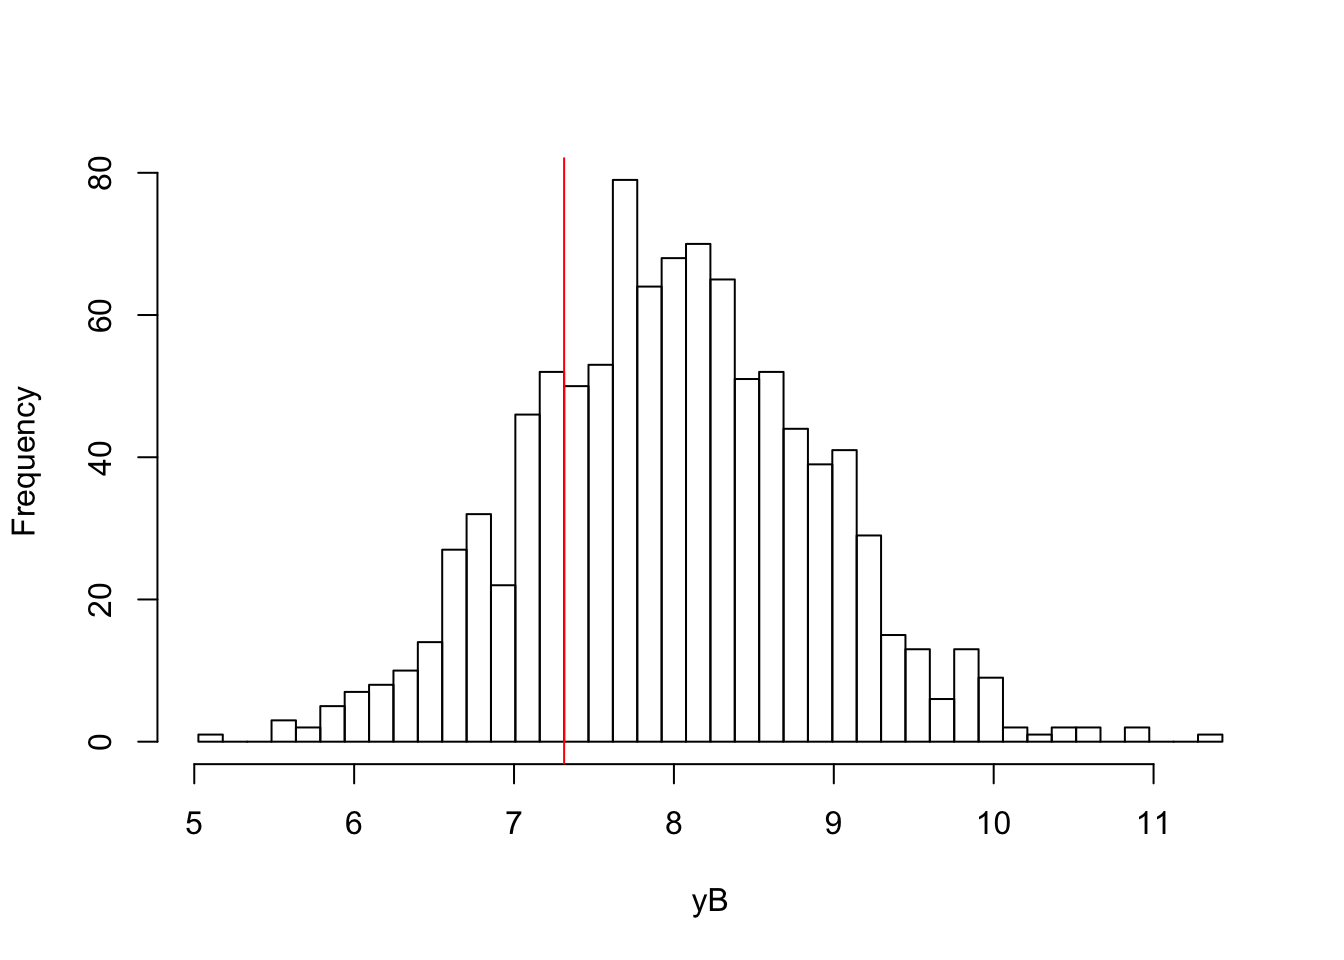
\includegraphics[width=0.6\linewidth]{STCI_files/figure-latex/histyb-1} 

}

\caption{Histogram of $y_B$}\label{fig:histyb}
\end{figure}

You can see on Figure \ref{fig:histyb} a histogram of \(y_i^B\) with the
red line indicating the cutoff point: \(\bar{y}=\ln(\bar{Y})=\) 7.3. All
the observations below the red line are treated according to the sharp
rule while all the one located above are not. In order to see how many
observations eventually receive the treatment with this allocation rule,
let's build a contingency table.

\begin{Shaded}
\begin{Highlighting}[]
\NormalTok{table.D.sharp <-}\StringTok{ }\KeywordTok{as.matrix}\NormalTok{(}\KeywordTok{table}\NormalTok{(Ds))}
\NormalTok{knitr}\OperatorTok{::}\KeywordTok{kable}\NormalTok{(table.D.sharp,}\DataTypeTok{caption=}\StringTok{'Treatment allocation with sharp cutoff rule'}\NormalTok{,}\DataTypeTok{booktabs=}\OtherTok{TRUE}\NormalTok{)}
\end{Highlighting}
\end{Shaded}

\begin{table}[t]

\caption{\label{tab:tableDsharp}Treatment allocation with sharp cutoff rule}
\centering
\begin{tabular}{lr}
\toprule
0 & 769\\
1 & 231\\
\bottomrule
\end{tabular}
\end{table}

We can see on Table \ref{tab:tableDsharp} that there are 231 treated
observations.

\subsubsection{Fuzzy cutoff rule}\label{fuzzy-cutoff-rule}

This rule is less sharp than the sharp cutoff rule. Here, other criteria
than \(Y_i^B\) enter into the decision to allocate the treatment. The
doctor might measure the health status of a patient following official
guidelines, but he might also measure other factors that will also
influence his decision of giving the drug to the patient. The officials
administering a program might measure the official income level of a
household, but they might also consider other features of the household
situation when deciding to enroll the household into the program or not.
If these additional criteria are unobserved to the econometrician, then
we have the fuzzy cutoff rule. A very simple way to model this rule is
as follows:

\begin{align}\label{eq:fuzzcutoff}
  D_i & = \uns{Y_i^B+V_i\leq\bar{Y}},
\end{align}

where \(V_i\) is a random variable unobserved to the econometrician and
standing for the other influences that might drive the allocation of the
treatment. \(V_i\) is distributed according to a, for the moment,
unspecified cumulative distribution function \(F_V\). When \(V_i\) is
degenerate (\textit{i.e.} it has only one point of support: it is a
constant), the fuzzy cutoff rule becomes the sharp cutoff rule.

\subsubsection{\texorpdfstring{Eligibility \(+\) self-selection
rule}{Eligibility + self-selection rule}}\label{eligibility-self-selection-rule}

It is also possible that households, once they have been made eligible
to the treatment, can decide whether they want to receive it or not. A
patient might be able to refuse the drug that the doctor suggests she
should take. A household might refuse to participate in a cash transfer
program to which it has been made eligible. Not all programs have this
feature, but most of them have some room for decisions by the agents
themselves of whether they want to receive the treatment or not. One
simple way to model this rule is as follows:

\begin{align}\label{eq:eligself}
  D_i & = \uns{D^*_i\geq0}E_i,
\end{align}

where \(D^*_i\) is individual \(i\)'s valuation of the treatment and
\(E_i\) is whether or not she is deemed eligible for the treatment.
\(E_i\) might be choosen according to the sharp cutoff rule of to the
fuzzy cutoff rule, or to any other eligibility rule. We will be more
explicit about \(D_i^*\) in what follows.

\textbf{SIMULATIONS ARE MISSING FOR THESE LAST TWO RULES}

\subsection{Potential outcomes}\label{potential-outcomes}

The second main building block of RCM are potential outcomes. Let's say
that we are interested in the effect of a treatment on an outcome \(Y\).
Each unit \(i\) can thus be in two potential states: treated or non
treated. Before the allocation of the treatment is decided, both of
these states are feasible for each unit.

\BeginKnitrBlock{definition}[Potential outcomes]
\protect\hypertarget{def:unnamed-chunk-2}{}{\label{def:unnamed-chunk-2}
\iffalse (Potential outcomes) \fi{} }For each unit \(i\), we define two
potential outcomes:
\EndKnitrBlock{definition}

\begin{itemize}
\tightlist
\item
  \(Y_i^1\): the outcome that unit \(i\) is going to have if it receives
  the treatment,
\item
  \(Y_i^0\): the outcome that unit \(i\) is going to have if it
  \textbf{does not} receive the treatment.
\end{itemize}

\BeginKnitrBlock{example}
\protect\hypertarget{exm:unnamed-chunk-3}{}{\label{exm:unnamed-chunk-3}
}Let's choose functional forms for our potential outcomes. For
simplicity, all lower case letters will denote log outcomes.
\(y_i^0=\mu_i+\delta+U_i^0\), with \(\delta\) a time shock common to all
the observations and \(U_i^0=\rho U_i^B+\epsilon_i\), with \(|\rho|<1\).
In the absence of the treatment, part of the shocks \(U_i^B\) that the
individuals experienced in the previous period persist, while some part
vanish. \(y_i^1=y_i^0+\bar{\alpha}+\theta\mu_i+\eta_i\). In order to
generate the potential outcomes, one has to define the laws for the
shocks and to choose parameter values. Let's assume that
\(\epsilon_i\sim\mathcal{N}(0,\sigma^2_{\epsilon})\) and
\(\eta_i\sim\mathcal{N}(0,\sigma^2_{\eta})\). Now let's choose some
parameter values:
\EndKnitrBlock{example}

\begin{Shaded}
\begin{Highlighting}[]
\NormalTok{l <-}\StringTok{ }\KeywordTok{length}\NormalTok{(param)}
\NormalTok{param <-}\StringTok{ }\KeywordTok{c}\NormalTok{(param,}\FloatTok{0.9}\NormalTok{,}\FloatTok{0.01}\NormalTok{,}\FloatTok{0.05}\NormalTok{,}\FloatTok{0.05}\NormalTok{,}\FloatTok{0.05}\NormalTok{,}\FloatTok{0.1}\NormalTok{)}
\KeywordTok{names}\NormalTok{(param)[(l}\OperatorTok{+}\DecValTok{1}\NormalTok{)}\OperatorTok{:}\KeywordTok{length}\NormalTok{(param)] <-}\StringTok{ }\KeywordTok{c}\NormalTok{(}\StringTok{"rho"}\NormalTok{,}\StringTok{"theta"}\NormalTok{,}\StringTok{"sigma2epsilon"}\NormalTok{,}\StringTok{"sigma2eta"}\NormalTok{,}\StringTok{"delta"}\NormalTok{,}\StringTok{"baralpha"}\NormalTok{)}
\NormalTok{param}
\end{Highlighting}
\end{Shaded}

\begin{verbatim}
##         barmu      sigma2mu       sigma2U          barY           rho 
##          8.00          0.50          0.28       1500.00          0.90 
##         theta sigma2epsilon     sigma2eta         delta      baralpha 
##          0.01          0.05          0.05          0.05          0.10
\end{verbatim}

We can finally generate the potential outcomes;

\begin{Shaded}
\begin{Highlighting}[]
\NormalTok{epsilon <-}\StringTok{ }\KeywordTok{rnorm}\NormalTok{(N,}\DecValTok{0}\NormalTok{,}\KeywordTok{sqrt}\NormalTok{(param[}\StringTok{"sigma2epsilon"}\NormalTok{]))}
\NormalTok{eta<-}\StringTok{ }\KeywordTok{rnorm}\NormalTok{(N,}\DecValTok{0}\NormalTok{,}\KeywordTok{sqrt}\NormalTok{(param[}\StringTok{"sigma2eta"}\NormalTok{]))}
\NormalTok{U0 <-}\StringTok{ }\NormalTok{param[}\StringTok{"rho"}\NormalTok{]}\OperatorTok{*}\NormalTok{UB }\OperatorTok{+}\StringTok{ }\NormalTok{epsilon}
\NormalTok{y0 <-}\StringTok{ }\NormalTok{mu }\OperatorTok{+}\StringTok{  }\NormalTok{U0 }\OperatorTok{+}\StringTok{ }\NormalTok{param[}\StringTok{"delta"}\NormalTok{]}
\NormalTok{alpha <-}\StringTok{ }\NormalTok{param[}\StringTok{"baralpha"}\NormalTok{]}\OperatorTok{+}\StringTok{  }\NormalTok{param[}\StringTok{"theta"}\NormalTok{]}\OperatorTok{*}\NormalTok{mu }\OperatorTok{+}\StringTok{ }\NormalTok{eta}
\NormalTok{y1 <-}\StringTok{ }\NormalTok{y0}\OperatorTok{+}\NormalTok{alpha}
\NormalTok{Y0 <-}\StringTok{ }\KeywordTok{exp}\NormalTok{(y0)}
\NormalTok{Y1 <-}\StringTok{ }\KeywordTok{exp}\NormalTok{(y1)}
\end{Highlighting}
\end{Shaded}

Now, I would like to visualize my potential outcomes:

\begin{Shaded}
\begin{Highlighting}[]
\KeywordTok{plot}\NormalTok{(y0,y1)}
\end{Highlighting}
\end{Shaded}

\begin{figure}

{\centering 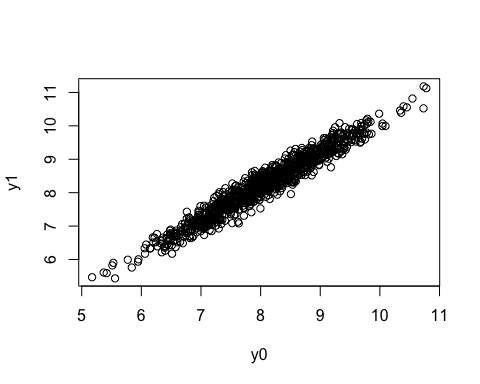
\includegraphics[width=0.6\linewidth]{STCI_files/figure-latex/histpotout-1} 

}

\caption{Potential outcomes}\label{fig:histpotout}
\end{figure}

You can see on the resulting Figure \ref{fig:histpotout} that both
potential outcomes are positively correlated. Those with a large
potential outcome when untreated (\emph{e.g.} in good health without the
treatment) also have a positive health with the treatment. It is also
true that individuals with bad health in the absence of the treatment
also have bad health with the treatment.

\subsection{Switching equation}\label{switching-equation}

The last building block of RCM is the switching equation. It links the
observed outcome to the potential outcomes through the allocation rule:

\begin{align}
 \label{eq:switch}
  Y_i & = 
    \begin{cases}
    Y_i^1 & \text{if } D_i=1\\
    Y_i^0 & \text{if } D_i=0
    \end{cases} \\
    & = Y_i^1D_i + Y_i^0(1-D_i) \nonumber
\end{align}

\BeginKnitrBlock{example}
\protect\hypertarget{exm:unnamed-chunk-4}{}{\label{exm:unnamed-chunk-4} }In
order to generate observed outcomes in our numerical example, we simply
have to enforce the switching equation:
\EndKnitrBlock{example}

\begin{Shaded}
\begin{Highlighting}[]
\NormalTok{y <-}\StringTok{ }\NormalTok{y1}\OperatorTok{*}\NormalTok{Ds}\OperatorTok{+}\NormalTok{y0}\OperatorTok{*}\NormalTok{(}\DecValTok{1}\OperatorTok{-}\NormalTok{Ds)}
\NormalTok{Y <-}\StringTok{ }\NormalTok{Y1}\OperatorTok{*}\NormalTok{Ds}\OperatorTok{+}\NormalTok{Y0}\OperatorTok{*}\NormalTok{(}\DecValTok{1}\OperatorTok{-}\NormalTok{Ds)}
\end{Highlighting}
\end{Shaded}

What the switching equation \eqref{eq:switch} means is that, for each
individual \(i\), we get to observe only one of the two potential
outcomes. When individual \(i\) belongs to the treatment group
(\emph{i.e.} \(D_i=1\)), we get to observe \(Y_i^1\). When individual
\(i\) belongs to the control group (\emph{i.e.} \(D_i=0\)), we get to
observe \(Y_i^0\). Because the same individual cannot be at the same
time in both groups, we can NEVER see both potential outcomes for the
same individual at the same time.

For each of the individuals, one of the two potential outcomes is
unobserved. We say that it is a \textbf{counterfactual}. A
counterfactual quantity is a quantity that is, according to Hume's
definition, contrary to the observed facts. A counterfactual cannot be
observed, but it can be conceived by an effort of reason: it is the
consequence of what would have happened had some action not been taken.

\BeginKnitrBlock{remark}
\iffalse{} {Remark. } \fi{}One very nice way of visualising the
switching equation has been proposed by Jerzy Neyman in a 1923 prescient
paper. Neyman proposes to imagine two urns, each one filled with \(N\)
balls. One urn is the treatment urn and contains balls with the id of
the unit and the value of its potential outcome \(Y_i^1\). The other urn
is the control urn, and it contains balls with the value of the
potential outcome \(Y_i^0\) for each unit \(i\). Following the
allocation rule \(D_i\), we decide whether unit \(i\) is in the
treatment or control group. When unit \(i\) is in the treatment group,
we take the corresponding ball from the first urn and observe the
potential outcome on it. But, at the same time, the urns are connected
so that the corresponding ball with the potential outcome of unit \(i\)
in the control urn disappears as soon as we draw ball \(i\) from the
treatment urn.

The switching equation works a lot like Schrodinger's cat paradox.
Schrodinger's cat is placed in a sealed box and receives a dose of
poison when an atom emits a radiation. As long as the box is sealed,
there is no way we can know whether the cat is dead or alive. When we
open the box, we observe either a dead cat or a living cat, but we
cannot observe the cat both alive and dead at the same time. The
switching equation is like opening the box, it collapses the observed
outcome into one of the two potential ones.
\EndKnitrBlock{remark}

\BeginKnitrBlock{example}
\protect\hypertarget{exm:unnamed-chunk-6}{}{\label{exm:unnamed-chunk-6} }One
way to visualize the inner workings of the switching equation is to plot
the potential outcomes along with the criteria driving the allocation
rule. In our simple example, it simply amounts to plotting observed
(\(y_i\)) and potential outcomes (\(y_i^1\) and \(y_i^0\)) along
\(y_i^B\).
\EndKnitrBlock{example}

\begin{Shaded}
\begin{Highlighting}[]
\KeywordTok{plot}\NormalTok{(yB[Ds}\OperatorTok{==}\DecValTok{0}\NormalTok{],y0[Ds}\OperatorTok{==}\DecValTok{0}\NormalTok{],}\DataTypeTok{pch=}\DecValTok{1}\NormalTok{,}\DataTypeTok{xlim=}\KeywordTok{c}\NormalTok{(}\DecValTok{5}\NormalTok{,}\DecValTok{11}\NormalTok{),}\DataTypeTok{ylim=}\KeywordTok{c}\NormalTok{(}\DecValTok{5}\NormalTok{,}\DecValTok{11}\NormalTok{),}\DataTypeTok{xlab=}\StringTok{"yB"}\NormalTok{,}\DataTypeTok{ylab=}\StringTok{"Outcomes"}\NormalTok{)}
\KeywordTok{points}\NormalTok{(yB[Ds}\OperatorTok{==}\DecValTok{1}\NormalTok{],y1[Ds}\OperatorTok{==}\DecValTok{1}\NormalTok{],}\DataTypeTok{pch=}\DecValTok{3}\NormalTok{)}
\KeywordTok{points}\NormalTok{(yB[Ds}\OperatorTok{==}\DecValTok{0}\NormalTok{],y1[Ds}\OperatorTok{==}\DecValTok{0}\NormalTok{],}\DataTypeTok{pch=}\DecValTok{3}\NormalTok{,}\DataTypeTok{col=}\StringTok{'red'}\NormalTok{)}
\KeywordTok{points}\NormalTok{(yB[Ds}\OperatorTok{==}\DecValTok{1}\NormalTok{],y0[Ds}\OperatorTok{==}\DecValTok{1}\NormalTok{],}\DataTypeTok{pch=}\DecValTok{1}\NormalTok{,}\DataTypeTok{col=}\StringTok{'red'}\NormalTok{)}
\NormalTok{test <-}\StringTok{ }\FloatTok{5.8}
\NormalTok{i.test <-}\StringTok{ }\KeywordTok{which}\NormalTok{(}\KeywordTok{abs}\NormalTok{(yB}\OperatorTok{-}\NormalTok{test)}\OperatorTok{==}\KeywordTok{min}\NormalTok{(}\KeywordTok{abs}\NormalTok{(yB}\OperatorTok{-}\NormalTok{test)))}
\KeywordTok{points}\NormalTok{(yB[}\KeywordTok{abs}\NormalTok{(yB}\OperatorTok{-}\NormalTok{test)}\OperatorTok{==}\KeywordTok{min}\NormalTok{(}\KeywordTok{abs}\NormalTok{(yB}\OperatorTok{-}\NormalTok{test))],y1[}\KeywordTok{abs}\NormalTok{(yB}\OperatorTok{-}\NormalTok{test)}\OperatorTok{==}\KeywordTok{min}\NormalTok{(}\KeywordTok{abs}\NormalTok{(yB}\OperatorTok{-}\NormalTok{test))],}\DataTypeTok{col=}\StringTok{'green'}\NormalTok{,}\DataTypeTok{pch=}\DecValTok{3}\NormalTok{)}
\KeywordTok{points}\NormalTok{(yB[}\KeywordTok{abs}\NormalTok{(yB}\OperatorTok{-}\NormalTok{test)}\OperatorTok{==}\KeywordTok{min}\NormalTok{(}\KeywordTok{abs}\NormalTok{(yB}\OperatorTok{-}\NormalTok{test))],y0[}\KeywordTok{abs}\NormalTok{(yB}\OperatorTok{-}\NormalTok{test)}\OperatorTok{==}\KeywordTok{min}\NormalTok{(}\KeywordTok{abs}\NormalTok{(yB}\OperatorTok{-}\NormalTok{test))],}\DataTypeTok{col=}\StringTok{'green'}\NormalTok{)}
\KeywordTok{abline}\NormalTok{(}\DataTypeTok{v=}\KeywordTok{log}\NormalTok{(param[}\StringTok{"barY"}\NormalTok{]),}\DataTypeTok{col=}\StringTok{"red"}\NormalTok{)}
\KeywordTok{legend}\NormalTok{(}\DecValTok{5}\NormalTok{,}\DecValTok{11}\NormalTok{,}\KeywordTok{c}\NormalTok{(}\StringTok{'y0|D=0'}\NormalTok{,}\StringTok{'y1|D=1'}\NormalTok{,}\StringTok{'y0|D=1'}\NormalTok{,}\StringTok{'y1|D=0'}\NormalTok{,}\KeywordTok{paste}\NormalTok{(}\StringTok{'y0'}\NormalTok{,i.test,}\DataTypeTok{sep=}\StringTok{''}\NormalTok{),}\KeywordTok{paste}\NormalTok{(}\StringTok{'y1'}\NormalTok{,i.test,}\DataTypeTok{sep=}\StringTok{''}\NormalTok{)),}\DataTypeTok{pch=}\KeywordTok{c}\NormalTok{(}\DecValTok{1}\NormalTok{,}\DecValTok{3}\NormalTok{,}\DecValTok{1}\NormalTok{,}\DecValTok{3}\NormalTok{,}\DecValTok{1}\NormalTok{,}\DecValTok{3}\NormalTok{),}\DataTypeTok{col=}\KeywordTok{c}\NormalTok{(}\StringTok{'black'}\NormalTok{,}\StringTok{'black'}\NormalTok{,}\StringTok{'red'}\NormalTok{,}\StringTok{'red'}\NormalTok{,}\StringTok{'green'}\NormalTok{,}\StringTok{'green'}\NormalTok{),}\DataTypeTok{ncol=}\DecValTok{3}\NormalTok{)}
\end{Highlighting}
\end{Shaded}

\begin{figure}

{\centering 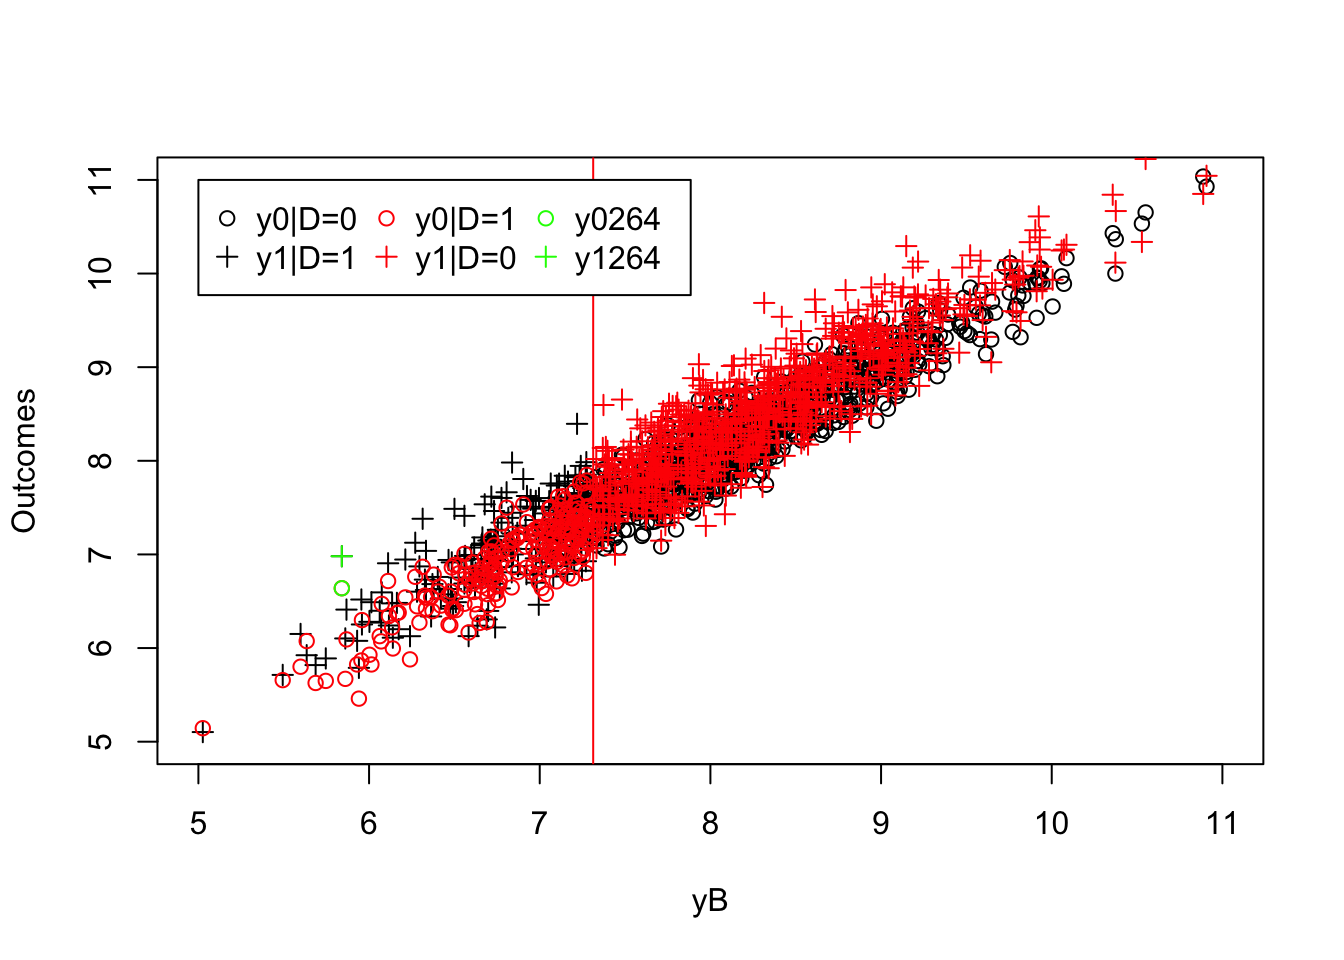
\includegraphics[width=0.6\linewidth]{STCI_files/figure-latex/ploty1y0yB-1} 

}

\caption{Potential outcomes}\label{fig:ploty1y0yB}
\end{figure}

\begin{Shaded}
\begin{Highlighting}[]
\KeywordTok{plot}\NormalTok{(yB[Ds}\OperatorTok{==}\DecValTok{0}\NormalTok{],y0[Ds}\OperatorTok{==}\DecValTok{0}\NormalTok{],}\DataTypeTok{pch=}\DecValTok{1}\NormalTok{,}\DataTypeTok{xlim=}\KeywordTok{c}\NormalTok{(}\DecValTok{5}\NormalTok{,}\DecValTok{11}\NormalTok{),}\DataTypeTok{ylim=}\KeywordTok{c}\NormalTok{(}\DecValTok{5}\NormalTok{,}\DecValTok{11}\NormalTok{),}\DataTypeTok{xlab=}\StringTok{"yB"}\NormalTok{,}\DataTypeTok{ylab=}\StringTok{"Outcomes"}\NormalTok{)}
\KeywordTok{points}\NormalTok{(yB[Ds}\OperatorTok{==}\DecValTok{1}\NormalTok{],y1[Ds}\OperatorTok{==}\DecValTok{1}\NormalTok{],}\DataTypeTok{pch=}\DecValTok{3}\NormalTok{)}
\KeywordTok{legend}\NormalTok{(}\DecValTok{5}\NormalTok{,}\DecValTok{11}\NormalTok{,}\KeywordTok{c}\NormalTok{(}\StringTok{'y|D=0'}\NormalTok{,}\StringTok{'y|D=1'}\NormalTok{),}\DataTypeTok{pch=}\KeywordTok{c}\NormalTok{(}\DecValTok{1}\NormalTok{,}\DecValTok{3}\NormalTok{))}
\KeywordTok{abline}\NormalTok{(}\DataTypeTok{v=}\KeywordTok{log}\NormalTok{(param[}\StringTok{"barY"}\NormalTok{]),}\DataTypeTok{col=}\StringTok{"red"}\NormalTok{)}
\end{Highlighting}
\end{Shaded}

\begin{figure}

{\centering 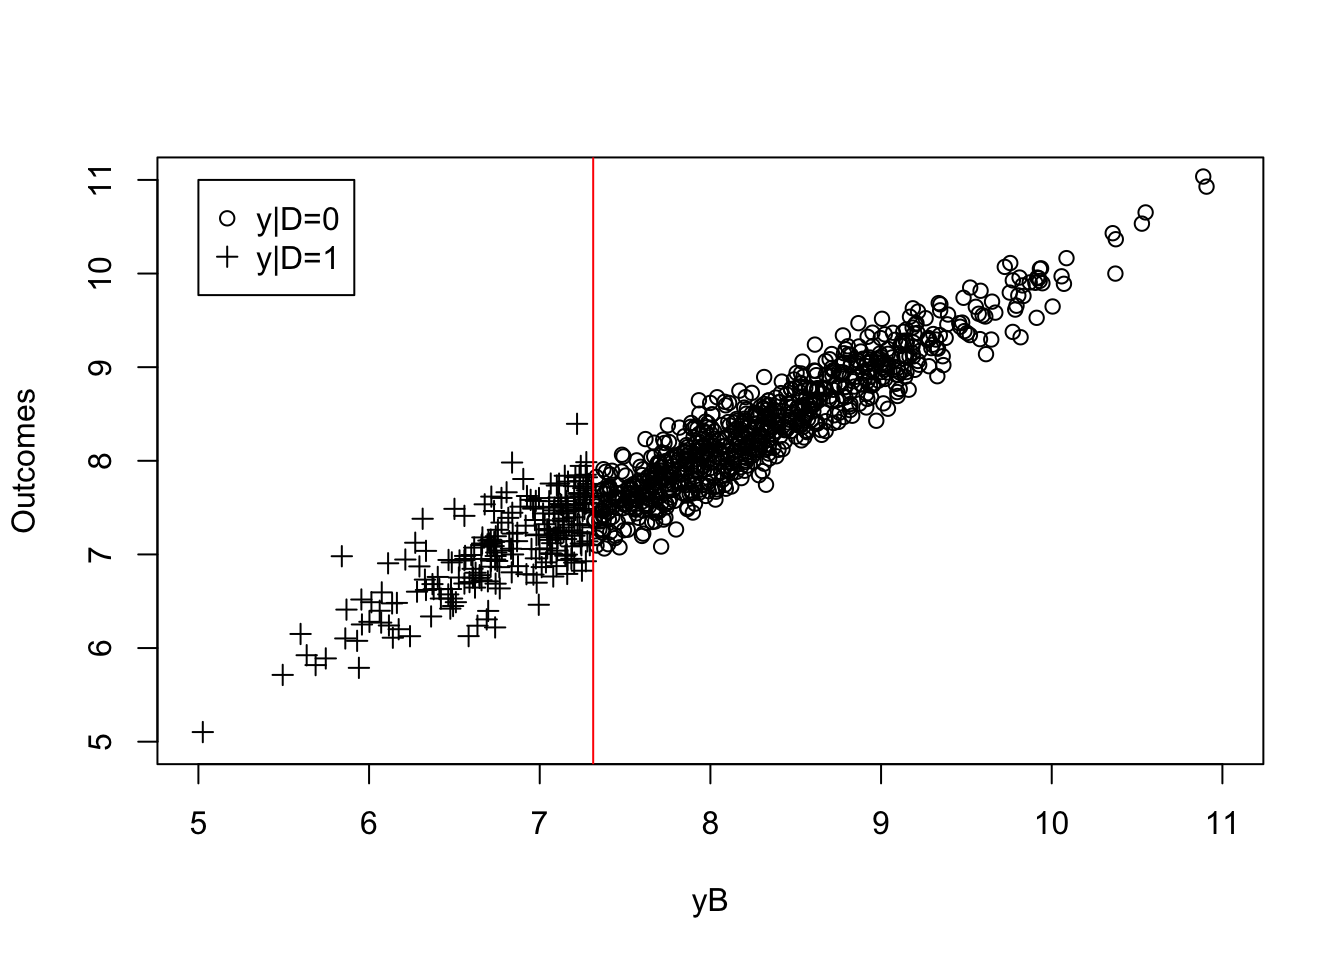
\includegraphics[width=0.6\linewidth]{STCI_files/figure-latex/plotyyB-1} 

}

\caption{Observed outcomes}\label{fig:plotyyB}
\end{figure}

Figure \ref{fig:ploty1y0yB} plots the observed outcomes \(y_i\) along
with the unobserved potential outcomes. Figure \ref{fig:ploty1y0yB}
shows that each individual in the sample is endowed with two potential
outcomes, represented by a circle and a cross. Figure \ref{fig:plotyyB}
plots the observed outcomes \(y_i\) that results from applying the
switching equation. Only one of the two potential outcomes is observed
(the cross for the treated group and the circle for the untreated group)
and the other is not. The observed sample in Figure \ref{fig:plotyyB}
only shows observed outcomes, and is thus silent on the values of the
missing potential outcomes.

\section{Treatment effects}\label{treatment-effects}

RCM enables the definition of causal effects at the individual level. In
practice though, we generally focus on a summary measure: the effect of
the treatment on the treated.

\subsection{Individual level treatment
effects}\label{individual-level-treatment-effects}

Potential outcomes enable us to define the central notion of causal
inference: the causal effect, also labelled the treatment effect, which
is the difference between the two potential outcomes.

\BeginKnitrBlock{definition}[Individual level treatment effect]
\protect\hypertarget{def:causaleff}{}{\label{def:causaleff}
\iffalse (Individual level treatment effect) \fi{} }For each unit \(i\),
the causal effect of the treatment on outcome \(Y\) is:
\(\Delta^Y_i=Y_i^1-Y_i^0\).
\EndKnitrBlock{definition}

\BeginKnitrBlock{example}
\protect\hypertarget{exm:unnamed-chunk-7}{}{\label{exm:unnamed-chunk-7} }The
individual level causal effect in log terms is:
\(\Delta^y_i=\alpha_i=\bar{\alpha}+\theta\mu_i+\eta_i\). The effect is
the sum of a part common to all individuals, a part correlated with
\(\mu_i\): the treatment might have a larger or a smaller effect
depending on the unobserved permanent ability or health status of
individuals, and a random shock. It is possible to make the effect of
the treatment to depend on \(U_i^B\) also, but it would complicate the
model.
\EndKnitrBlock{example}

In Figure \ref{fig:ploty1y0yB}, the individual level treatment effects
are the differences between each cross and its corresponding circle. For
example, for observation 938, the two potential outcomes appear in green
in Figure \ref{fig:ploty1y0yB}. The effect of the treatment on unit 938
is equal to: \[
\Delta^y_{938}=y^1_{938}-y^0_{938}=6.01-5.95=0.05.
\]

Since observation 938 belongs to the treatment group, we can only
observe the potential outcome in the presence of the treatment,
\(y^1_{938}\).

RCM allows for heterogeneity of treatment effects. The treatment has a
large effect on some units and a much smaller effect on other units. We
can even have some units that benefit from the treatment and some units
that are harmed by the treatment. The individual level effect of the
treatment is itself a random variable (and not a fixed parameter). It
has a distribution, \(F_{\Delta^Y}\).

Heterogeneity of treatment effects seems very natural: the treatment
might interact with individuals' different backgrounds. The effect of a
drug might depend on the genetic background of an individual. An
education program might only work for children that already have
sufficient non-cognitive skills, and thus might depend in turn on family
background. An environmental regulation or a behavioral intervention
might only trigger reactions by already environmentally aware
individuals. A CCT might have a larger effect when indiviuals are
credit-constrained or face shocks.

\BeginKnitrBlock{example}
\protect\hypertarget{exm:unnamed-chunk-8}{}{\label{exm:unnamed-chunk-8} }In
our numerical example, the distribution of \(\Delta^y_i=\alpha_i\) is a
normal:
\(\alpha_i\sim\mathcal{N}(\bar{\alpha}+\theta\bar{\mu},\theta^2\sigma^2_{\mu}+\sigma^2_{\eta})\).
We would like to visualize treatment effect heterogeneity. For that, we
can build a histogram of the individual level causal effect.
\EndKnitrBlock{example} On top of the histogram, we can also draw the
theoretical distribution of the treatment effect: a normal with mean
0.18 and variance 0.05.

\begin{Shaded}
\begin{Highlighting}[]
\KeywordTok{hist}\NormalTok{(alpha,}\DataTypeTok{main=}\StringTok{""}\NormalTok{,}\DataTypeTok{prob=}\OtherTok{TRUE}\NormalTok{)}
\KeywordTok{curve}\NormalTok{(}\KeywordTok{dnorm}\NormalTok{(x, }\DataTypeTok{mean=}\NormalTok{(param[}\StringTok{"baralpha"}\NormalTok{]}\OperatorTok{+}\NormalTok{param[}\StringTok{"theta"}\NormalTok{]}\OperatorTok{*}\NormalTok{param[}\StringTok{"barmu"}\NormalTok{]), }\DataTypeTok{sd=}\KeywordTok{sqrt}\NormalTok{(param[}\StringTok{"theta"}\NormalTok{]}\OperatorTok{^}\DecValTok{2}\OperatorTok{*}\NormalTok{param[}\StringTok{"sigma2mu"}\NormalTok{]}\OperatorTok{+}\NormalTok{param[}\StringTok{"sigma2eta"}\NormalTok{])), }\DataTypeTok{add=}\OtherTok{TRUE}\NormalTok{,}\DataTypeTok{col=}\StringTok{'red'}\NormalTok{)}
\end{Highlighting}
\end{Shaded}

\begin{figure}[htbp]

{\centering 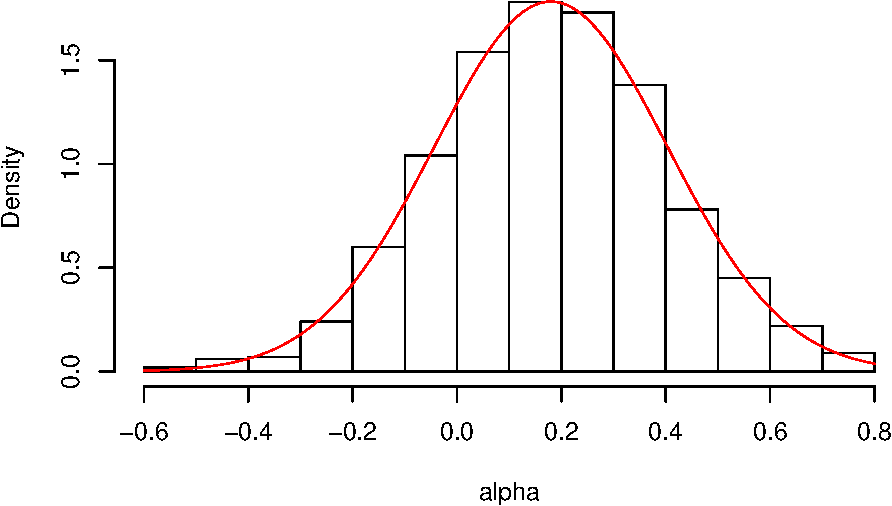
\includegraphics[width=0.6\linewidth]{STCI_files/figure-latex/histalpha-1} 

}

\caption{Histogram of $\Delta^y$}\label{fig:histalpha}
\end{figure}

The first thing that we can see on Figure \ref{fig:histalpha} is that
the theoretical and the empirical distributions nicely align with each
other. We also see that the majority of the observations lies to the
right of zero: most people experience a positive effect of the
treatment. But there are some individuals that do not benefit from the
treatment: the effect of the treatment on them is negative.

\subsection{Average treatment effect on the
treated}\label{average-treatment-effect-on-the-treated}

We do not generally estimate individual-level treatment effects. We
generally look for summary statistics of the effect of the treatment. By
far the most widely reported causal parameter is the Treatment on the
Treated parameter (TT). It can be defined in the sample at hand or in
the population.

\BeginKnitrBlock{definition}[Average and expected treatment effects on the treated]
\protect\hypertarget{def:TT}{}{\label{def:TT} \iffalse (Average and expected
treatment effects on the treated) \fi{} }The Treatment on the Treated
parameters for outcome \(Y\) are:
\EndKnitrBlock{definition}

\begin{itemize}
\tightlist
\item
  The average Treatment effect on the Treated in the sample:
\end{itemize}

\begin{align*}
  \Delta^Y_{TT_s} & = \frac{1}{\sum_{i=1}^ND_i}\sum_{i=1}^N(Y_i^1-Y_i^0)D_i,
  \end{align*}

\begin{itemize}
\tightlist
\item
  The expected Treatment effect on the Treated in the population:
\end{itemize}

\begin{align*}
  \Delta^Y_{TT} & = \esp{Y_i^1-Y_i^0|D_i=1}.
  \end{align*}

The TT parameters measure the average effect of the treatment on those
who actually take it, either in the sample at hand or in the popluation.
It is generally considered to be the most policy-relevant parameter
since it measures the effect of the treatment as it has actually been
allocated. For example, the expected causal effect on the overall
population is only relevant if policymakers are considering implementing
the treatment even on those who have not been selected to receive it.
For a drug or an anti-poverty program, it would mean giving the
treatment to healthy or rich people, which would make little sense.

TT does not say anything about how the effect of the treatment is
distributed in the population or in the sample. TT does not account for
the heterogneity of treatment effects. In Lecture 7, we will look at
other parameters of interest that look more closely into how the effect
of the treatment is distributed.

\BeginKnitrBlock{example}
\protect\hypertarget{exm:unnamed-chunk-9}{}{\label{exm:unnamed-chunk-9} }The
value of TT in our sample is:
\EndKnitrBlock{example} \[
\Delta^y_{TT_s}=0.158.
\]

Computing the population value of \(TT\) is slightly more involved: we
have to use the formula for the conditional expectation of a censored
bivariate normal random variable:

\begin{align*}
\Delta^y_{TT} & = \esp{\alpha_i|D_i=1}\\
              & = \bar{\alpha}+\theta\esp{\mu_i|\mu_i+U_i^B\leq\bar{y}}\\
              & = \bar{\alpha}+\theta\left(\bar{\mu} - \frac{\sigma^2_{\mu}}{\sqrt{\sigma^2_{\mu}+\sigma^2_{U}}}\frac{\phi\left(\frac{\bar{y}-\bar{\mu}}{\sqrt{\sigma^2_{\mu}+\sigma^2_{U}}}\right)}{\Phi\left(\frac{\bar{y}-\bar{\mu}}{\sqrt{\sigma^2_{\mu}+\sigma^2_{U}}}\right)}\right)\\
              & = \bar{\alpha}+\theta\bar{\mu}-\theta\left(\frac{\sigma^2_{\mu}}{\sqrt{\sigma^2_{\mu}+\sigma^2_{U}}}\frac{\phi\left(\frac{\bar{y}-\bar{\mu}}{\sqrt{\sigma^2_{\mu}+\sigma^2_{U}}}\right)}{\Phi\left(\frac{\bar{y}-\bar{\mu}}{\sqrt{\sigma^2_{\mu}+\sigma^2_{U}}}\right)}\right),
\end{align*}

where \(\phi\) and \(\Phi\) are respectively the density and the
cumulative distribution functions of the standard normal. The second
equality follows from the definition of \(\alpha_i\) and \(D_i\) and
from the fact that \(\eta_i\) is independent from \(\mu_i\) and
\(U_i^B\). The third equality comes from the formula for the expectation
of a censored bivariate normal random variable. In order to compute the
population value of TT easily for different sets of parameter values,
let's write a function in R:

\begin{Shaded}
\begin{Highlighting}[]
\NormalTok{delta.y.tt <-}\StringTok{ }\ControlFlowTok{function}\NormalTok{(param)\{}\KeywordTok{return}\NormalTok{(param[}\StringTok{"baralpha"}\NormalTok{]}\OperatorTok{+}\NormalTok{param[}\StringTok{"theta"}\NormalTok{]}\OperatorTok{*}\NormalTok{param[}\StringTok{"barmu"}\NormalTok{]}
                                     \OperatorTok{-}\NormalTok{param[}\StringTok{"theta"}\NormalTok{]}\OperatorTok{*}\NormalTok{((param[}\StringTok{"sigma2mu"}\NormalTok{]}\OperatorTok{*}\KeywordTok{dnorm}\NormalTok{((}\KeywordTok{log}\NormalTok{(param[}\StringTok{"barY"}\NormalTok{])}\OperatorTok{-}\NormalTok{param[}\StringTok{"barmu"}\NormalTok{])}\OperatorTok{/}\NormalTok{(}\KeywordTok{sqrt}\NormalTok{(param[}\StringTok{"sigma2mu"}\NormalTok{]}\OperatorTok{+}\NormalTok{param[}\StringTok{"sigma2U"}\NormalTok{]))))}
                                                      \OperatorTok{/}\NormalTok{(}\KeywordTok{sqrt}\NormalTok{(param[}\StringTok{"sigma2mu"}\NormalTok{]}\OperatorTok{+}\NormalTok{param[}\StringTok{"sigma2U"}\NormalTok{])}
                                                        \OperatorTok{*}\KeywordTok{pnorm}\NormalTok{((}\KeywordTok{log}\NormalTok{(param[}\StringTok{"barY"}\NormalTok{])}\OperatorTok{-}\NormalTok{param[}\StringTok{"barmu"}\NormalTok{])}\OperatorTok{/}\NormalTok{(}\KeywordTok{sqrt}\NormalTok{(param[}\StringTok{"sigma2mu"}\NormalTok{]}\OperatorTok{+}\NormalTok{param[}\StringTok{"sigma2U"}\NormalTok{]))))))\}}
\end{Highlighting}
\end{Shaded}

The population value of TT computed using this function is:
\(\Delta^y_{TT}=\) 0.172. We can see that the values of TT in the sample
and in the population differ slightly. This is because of sampling
noise: the units in the sample are not perfectly representative of the
units in the population.

\section{Fundamental problem of causal
inference}\label{fundamental-problem-of-causal-inference}

At least in this lecture, causal inference is about trying to infer TT,
either in the sample or in the population. The FPCI states that it is
impossible to directly observe TT because one part of it remains
fundamentally unobserved.

\BeginKnitrBlock{theorem}[Fundamental problem of causal inference]
\protect\hypertarget{thm:FPCI}{}{\label{thm:FPCI} \iffalse (Fundamental
problem of causal inference) \fi{} }It is impossible to observe TT,
either in the population or in the sample.
\EndKnitrBlock{theorem}

\BeginKnitrBlock{proof}
\iffalse{} {Proof. } \fi{}The proof of the FPCI is rather
straightforward. Let me start with the sample TT:

\begin{align*}
  \Delta^Y_{TT_s} & = \frac{1}{\sum_{i=1}^ND_i}\sum_{i=1}^N(Y_i^1-Y_i^0)D_i \\
                  & = \frac{1}{\sum_{i=1}^ND_i}\sum_{i=1}^NY_i^1D_i- \frac{1}{\sum_{i=1}^ND_i}\sum_{i=1}^NY_i^0D_i \\
                  & = \frac{1}{\sum_{i=1}^ND_i}\sum_{i=1}^NY_iD_i- \frac{1}{\sum_{i=1}^ND_i}\sum_{i=1}^NY_i^0D_i.
\end{align*}

Since \(Y_i^0\) is unobserved whenever \(D_i=1\),
\(\frac{1}{\sum_{i=1}^ND_i}\sum_{i=1}^NY_i^0D_i\) is unobserved, and so
is \(\Delta^Y_{TT_s}\). The same is true for the population TT:

\begin{align*}
  \Delta^Y_{TT} & = \esp{Y_i^1-Y_i^0|D_i=1} \\
                & = \esp{Y_i^1|D_i=1}-\esp{Y_i^0|D_i=1}\\
                & = \esp{Y_i|D_i=1}-\esp{Y_i^0|D_i=1}.
\end{align*}

\(\esp{Y_i^0|D_i=1}\) is unobserved, and so is \(\Delta^Y_{TT}\).
\EndKnitrBlock{proof}

The key insight in order to understand the FPCI is to see that the
outcomes of the treated units had they not been treated are
unobservable, and so is their average or expectation. We say that they
are counterfactual, contrary to what has happened.

\BeginKnitrBlock{definition}[Couterfactual]
\protect\hypertarget{def:counter}{}{\label{def:counter}
\iffalse (Couterfactual) \fi{} }Both
\(\frac{1}{\sum_{i=1}^ND_i}\sum_{i=1}^NY_i^0D_i\) and
\(\esp{Y_i^0|D_i=1}\) are counterfactual quantities that we will never
get to observe.
\EndKnitrBlock{definition}

\BeginKnitrBlock{example}
\protect\hypertarget{exm:unnamed-chunk-11}{}{\label{exm:unnamed-chunk-11}
}The average counterfactual outcome of the treated is the mean of the
red circles in the \(y\) axis on Figure \ref{fig:ploty1y0yB}:
\EndKnitrBlock{example} \[
\frac{1}{\sum_{i=1}^ND_i}\sum_{i=1}^Ny_i^0D_i= 6.93.
\] Remember that we can estimate this quantity only because we have
generated the data ourselves. In real life, this quantity is hopelessly
unobserved.

\(\esp{y_i^0|D_i=1}\) can be computed using the formula for the
expectation of a censored normal random variable:

\begin{align*}
\esp{y_i^0|D_i=1} & = \esp{\mu_i+\delta+U_i^0|D_i=1}\\
                  & = \esp{\mu_i+\delta+\rho U_i^B+\epsilon_i|D_i=1}\\
                  & = \delta + \esp{\mu_i+\rho U_i^B|y_i^B\leq\bar{y}}\\
                  & = \delta + \bar{\mu} - \frac{\sigma^2_{\mu}+\rho\sigma^2_U}{\sqrt{\sigma^2_{\mu}+\sigma^2_{U}}}\frac{\phi\left(\frac{\bar{y}-\bar{\mu}}{\sqrt{\sigma^2_{\mu}+\sigma^2_{U}}}\right)}{\Phi\left(\frac{\bar{y}-\bar{\mu}}{\sqrt{\sigma^2_{\mu}+\sigma^2_{U}}}\right)}.
\end{align*}

We can write a function in R to compute this value:

\begin{Shaded}
\begin{Highlighting}[]
\NormalTok{esp.y0.D1 <-}\StringTok{ }\ControlFlowTok{function}\NormalTok{(param)\{}
  \KeywordTok{return}\NormalTok{(param[}\StringTok{"delta"}\NormalTok{]}\OperatorTok{+}\NormalTok{param[}\StringTok{"barmu"}\NormalTok{]}
         \OperatorTok{-}\NormalTok{((param[}\StringTok{"sigma2mu"}\NormalTok{]}\OperatorTok{+}\NormalTok{param[}\StringTok{"rho"}\NormalTok{]}\OperatorTok{*}\NormalTok{param[}\StringTok{"sigma2U"}\NormalTok{])}
           \OperatorTok{*}\KeywordTok{dnorm}\NormalTok{((}\KeywordTok{log}\NormalTok{(param[}\StringTok{"barY"}\NormalTok{])}\OperatorTok{-}\NormalTok{param[}\StringTok{"barmu"}\NormalTok{])}\OperatorTok{/}\NormalTok{(}\KeywordTok{sqrt}\NormalTok{(param[}\StringTok{"sigma2mu"}\NormalTok{]}\OperatorTok{+}\NormalTok{param[}\StringTok{"sigma2U"}\NormalTok{]))))}
         \OperatorTok{/}\NormalTok{(}\KeywordTok{sqrt}\NormalTok{(param[}\StringTok{"sigma2mu"}\NormalTok{]}\OperatorTok{+}\NormalTok{param[}\StringTok{"sigma2U"}\NormalTok{])}\OperatorTok{*}\KeywordTok{pnorm}\NormalTok{((}\KeywordTok{log}\NormalTok{(param[}\StringTok{"barY"}\NormalTok{])}\OperatorTok{-}\NormalTok{param[}\StringTok{"barmu"}\NormalTok{])}
                                                          \OperatorTok{/}\NormalTok{(}\KeywordTok{sqrt}\NormalTok{(param[}\StringTok{"sigma2mu"}\NormalTok{]}\OperatorTok{+}\NormalTok{param[}\StringTok{"sigma2U"}\NormalTok{])))))}
\NormalTok{\}}
\end{Highlighting}
\end{Shaded}

The population value of TT computed using this function is:
\(\esp{y_i^0|D_i=1}=\) 6.9.

\section{Intuitive estimators, confounding factors and selection
bias}\label{intuitive-estimators-confounding-factors-and-selection-bias}

In this section, we are going to examine the properties of two intuitive
comparisons that laypeople, policymakers but also ourselves make in
order to estimate causal effects: the with/wihtout comparison (\(WW\))
and the before/after comparison (\(BA\)). \(WW\) compares the average
outcomes of the treated individuals with those of the untreated
individuals. \(BA\) compares the average outcomes of the treated after
taking the treatment to their average outcomes before they took the
treatment. These comparisons try to proxy for the expected
counterfactual outcome in the treated group by using an observed
quantity. \(WW\) uses the expected outcome of the untreated individuals
as a proxy. \(BA\) uses the expected outcome of the treated before they
take the treatment as a proxy.

Unfortunately, both of these proxies are generally poor and provide
biased estimates of \(TT\). The reason that these proxies are poor is
that the treatment is not the only factor that differentiates the
treated group from the groups used to form the proxy. The intuitive
comparisons are biased because factors, other than the treatment, are
correlated to its allocation. The factors that bias the intuitive
comparisons are generally called confouding factors or confounders.

The treatment effect measures the effect of a ceteris paribus change in
treatment status, while the intuitive comparisons capture both the
effect of this change and that of other correlated changes that
spuriously contaminate the comparison. Intuitive comparisons measure
correlations while treatment effects measure causality. The old motto
``correlation is not causation'' applies vehemently here.

\BeginKnitrBlock{remark}
\iffalse{} {Remark. } \fi{}A funny anecdote about this expression
``correlation is not causation''. This expression is due to Karl
Pearson, the father of modern statistics. He coined the phrase in his
famous book ``The Grammar of Science.'' Pearson is famous for inventing
the correlation coefficient. He actually thought that correlation was a
much superior, much more rigorous term, than causation. In his book, he
actually used the sentence to argue in favor of abandoning causation
altogether and focusing on the much better-defined and measurable
concept of correlation. Interesting turn of events that his sentence is
now used to mean that correlation is weaker than causation, totally
reverting the original intended meaning.
\EndKnitrBlock{remark}

In this section, we are going to define both comparisons, study their
biases and state the conditions under which they identify \(TT\). This
will prove to be a very useful introduction to the notion of
identification. It is also very important to be able to understand the
sources of bias of comparisons that we use every day and that come very
naturally to policy makers and lay people.

\BeginKnitrBlock{remark}
\iffalse{} {Remark. } \fi{}In this section, we state the definitions and
formulae in the population. This is for two reasons. First, it is
simpler, and lighter in terms of notation. Second, it emphasizes that
the problems with intuitive comparisons are independent of sampling
noise. Most of the results stated here for the population extend to the
sample, replacing the expectation operator by the average operator. I
will nevertheless give examples in the sample, since it is so much
simpler to compute. I will denote sample equivalents of population
estimators with a hat.
\EndKnitrBlock{remark}

\subsection{With/Without comparison, selection bias and cross-sectional
confounders}\label{withwithout-comparison-selection-bias-and-cross-sectional-confounders}

The with/without comparison (\(WW\)) is very intuitive: just compare the
outcomes of the treated and untreated individuals in order to estimate
the causal effect. This approach is nevertheless generally biased. We
call the bias of \(WW\) selection bias (\(SB\)). Selection bias is due
to unobserved confounders that are distributed differently in the
treatment and control group and that generate differences in outcomes
even in the absence of the treatment. In this section, I define the
\(WW\) estimator, derives its bias, introduces the confounders and
states conditions under which it is unbiased.

\subsubsection{With/Without comparison}\label{withwithout-comparison}

The with/without comparison (\(WW\)) is very intuitive: just compare the
outcomes of the treated and untreated individuals in order to estimate
the causal effect.

\BeginKnitrBlock{definition}[With/without comparison]
\protect\hypertarget{def:unnamed-chunk-14}{}{\label{def:unnamed-chunk-14}
\iffalse (With/without comparison) \fi{} }The with/without comparison is
the difference between the expected outcomes of the treated and the
expected outcomes of the untreated:

\begin{align*}
\Delta^Y_{WW} & =  \esp{Y_i|D_i=1}-\esp{Y_i|D_i=0}.
\end{align*}
\EndKnitrBlock{definition}

\BeginKnitrBlock{example}
\protect\hypertarget{exm:unnamed-chunk-15}{}{\label{exm:unnamed-chunk-15}
}In the population, \(WW\) can be computed using the traditional formula
for the expectation of a truncated normal distribution:

\begin{align*}
\Delta^y_{WW} & = \esp{y_i|D_i=1}-\esp{y_i|D_i=0} \\
              & = \esp{y_i^1|D_i=1}-\esp{y^0_i|D_i=0} \\
              & = \esp{\alpha_i|D_i=1}+\esp{\mu_i+\rho U_i^B|\mu_i+U_i^B\leq\bar{y}}-\esp{\mu_i+\rho U_i^B|\mu_i+U_i^B>\bar{y}} \\
              & = \bar{\alpha}+\theta\left(\bar{\mu}-\frac{\sigma^2_{\mu}}{\sqrt{\sigma^2_{\mu}+\sigma^2_{U}}}\frac{\phi\left(\frac{\bar{y}-\bar{\mu}}{\sqrt{\sigma^2_{\mu}+\sigma^2_{U}}}\right)}{\Phi\left(\frac{\bar{y}-\bar{\mu}}{\sqrt{\sigma^2_{\mu}+\sigma^2_{U}}}\right)}\right)  
              -\frac{\sigma^2_{\mu}+\rho\sigma^2_{U}}{\sqrt{\sigma^2_{\mu}+\sigma^2_{U}}}\left(\frac{\phi\left(\frac{\bar{y}-\bar{\mu}}{\sqrt{\sigma^2_{\mu}+\sigma^2_{U}}}\right)}{\Phi\left(\frac{\bar{y}-\bar{\mu}}{\sqrt{\sigma^2_{\mu}+\sigma^2_{U}}}\right)}+\frac{\phi\left(\frac{\bar{y}-\bar{\mu}}{\sqrt{\sigma^2_{\mu}+\sigma^2_{U}}}\right)}{1-\Phi\left(\frac{\bar{y}-\bar{\mu}}{\sqrt{\sigma^2_{\mu}+\sigma^2_{U}}}\right)}\right).
\end{align*}
\EndKnitrBlock{example} In order to compute this parameter, we are going
to set up a R function. For reasons that will become clearer later, we
will define two separate functions to compute the first and second part
of the formula. In the first part, you should have recognised \(TT\),
that we have already computed in Lecture 1. We are going to call the
second part \(SB\), for reasons that will become explicit in a bit.

\begin{Shaded}
\begin{Highlighting}[]
\NormalTok{delta.y.tt <-}\StringTok{ }\ControlFlowTok{function}\NormalTok{(param)\{}
  \KeywordTok{return}\NormalTok{(param[}\StringTok{"baralpha"}\NormalTok{]}\OperatorTok{+}\NormalTok{param[}\StringTok{"theta"}\NormalTok{]}\OperatorTok{*}\NormalTok{param[}\StringTok{"barmu"}\NormalTok{]}\OperatorTok{-}\NormalTok{param[}\StringTok{"theta"}\NormalTok{]}
         \OperatorTok{*}\NormalTok{((param[}\StringTok{"sigma2mu"}\NormalTok{]}\OperatorTok{*}\KeywordTok{dnorm}\NormalTok{((}\KeywordTok{log}\NormalTok{(param[}\StringTok{"barY"}\NormalTok{])}\OperatorTok{-}\NormalTok{param[}\StringTok{"barmu"}\NormalTok{])}
                                    \OperatorTok{/}\NormalTok{(}\KeywordTok{sqrt}\NormalTok{(param[}\StringTok{"sigma2mu"}\NormalTok{]}\OperatorTok{+}\NormalTok{param[}\StringTok{"sigma2U"}\NormalTok{]))))}
           \OperatorTok{/}\NormalTok{(}\KeywordTok{sqrt}\NormalTok{(param[}\StringTok{"sigma2mu"}\NormalTok{]}\OperatorTok{+}\NormalTok{param[}\StringTok{"sigma2U"}\NormalTok{])}\OperatorTok{*}\KeywordTok{pnorm}\NormalTok{((}\KeywordTok{log}\NormalTok{(param[}\StringTok{"barY"}\NormalTok{])}\OperatorTok{-}\NormalTok{param[}\StringTok{"barmu"}\NormalTok{])}
                                                            \OperatorTok{/}\NormalTok{(}\KeywordTok{sqrt}\NormalTok{(param[}\StringTok{"sigma2mu"}\NormalTok{]}\OperatorTok{+}\NormalTok{param[}\StringTok{"sigma2U"}\NormalTok{]))))))}
\NormalTok{\}}
\NormalTok{delta.y.sb <-}\StringTok{ }\ControlFlowTok{function}\NormalTok{(param)\{}
  \KeywordTok{return}\NormalTok{(}\OperatorTok{-}\NormalTok{(param[}\StringTok{"sigma2mu"}\NormalTok{]}\OperatorTok{+}\NormalTok{param[}\StringTok{"rho"}\NormalTok{]}\OperatorTok{*}\NormalTok{param[}\StringTok{"sigma2U"}\NormalTok{])}\OperatorTok{/}\KeywordTok{sqrt}\NormalTok{(param[}\StringTok{"sigma2mu"}\NormalTok{]}\OperatorTok{+}\NormalTok{param[}\StringTok{"sigma2U"}\NormalTok{])}
         \OperatorTok{*}\KeywordTok{dnorm}\NormalTok{((}\KeywordTok{log}\NormalTok{(param[}\StringTok{"barY"}\NormalTok{])}\OperatorTok{-}\NormalTok{param[}\StringTok{"barmu"}\NormalTok{])}\OperatorTok{/}\NormalTok{(}\KeywordTok{sqrt}\NormalTok{(param[}\StringTok{"sigma2mu"}\NormalTok{]}\OperatorTok{+}\NormalTok{param[}\StringTok{"sigma2U"}\NormalTok{])))}
         \OperatorTok{*}\NormalTok{(}\DecValTok{1}\OperatorTok{/}\KeywordTok{pnorm}\NormalTok{((}\KeywordTok{log}\NormalTok{(param[}\StringTok{"barY"}\NormalTok{])}\OperatorTok{-}\NormalTok{param[}\StringTok{"barmu"}\NormalTok{])}\OperatorTok{/}\NormalTok{(}\KeywordTok{sqrt}\NormalTok{(param[}\StringTok{"sigma2mu"}\NormalTok{]}\OperatorTok{+}\NormalTok{param[}\StringTok{"sigma2U"}\NormalTok{])))}
           \OperatorTok{+}\DecValTok{1}\OperatorTok{/}\NormalTok{(}\DecValTok{1}\OperatorTok{-}\KeywordTok{pnorm}\NormalTok{((}\KeywordTok{log}\NormalTok{(param[}\StringTok{"barY"}\NormalTok{])}\OperatorTok{-}\NormalTok{param[}\StringTok{"barmu"}\NormalTok{])}\OperatorTok{/}\NormalTok{(}\KeywordTok{sqrt}\NormalTok{(param[}\StringTok{"sigma2mu"}\NormalTok{]}\OperatorTok{+}\NormalTok{param[}\StringTok{"sigma2U"}\NormalTok{]))))))}
\NormalTok{\}}
\NormalTok{delta.y.ww <-}\StringTok{ }\ControlFlowTok{function}\NormalTok{(param)\{}
  \KeywordTok{return}\NormalTok{(}\KeywordTok{delta.y.tt}\NormalTok{(param)}\OperatorTok{+}\KeywordTok{delta.y.sb}\NormalTok{(param))}
\NormalTok{\}}
\end{Highlighting}
\end{Shaded}

As a conclusion of all these derivations, \(WW\) in the population is
equal to -1.298. Remember that the value of \(TT\) in the population is
0.172.

In order to compute the \(WW\) estimator in a sample, I'm going to
generate a brand new sample and I'm going to choose a seed for the
pseudo-random number generator so that we obtain the same result each
time we run the code. I use \texttt{set.seed(1234)} in the code chunk
below.

\begin{Shaded}
\begin{Highlighting}[]
\NormalTok{param <-}\StringTok{ }\KeywordTok{c}\NormalTok{(}\DecValTok{8}\NormalTok{,.}\DecValTok{5}\NormalTok{,.}\DecValTok{28}\NormalTok{,}\DecValTok{1500}\NormalTok{)}
\KeywordTok{names}\NormalTok{(param) <-}\StringTok{ }\KeywordTok{c}\NormalTok{(}\StringTok{"barmu"}\NormalTok{,}\StringTok{"sigma2mu"}\NormalTok{,}\StringTok{"sigma2U"}\NormalTok{,}\StringTok{"barY"}\NormalTok{)}
\KeywordTok{set.seed}\NormalTok{(}\DecValTok{1234}\NormalTok{)}
\NormalTok{N <-}\DecValTok{1000}
\NormalTok{mu <-}\StringTok{ }\KeywordTok{rnorm}\NormalTok{(N,param[}\StringTok{"barmu"}\NormalTok{],}\KeywordTok{sqrt}\NormalTok{(param[}\StringTok{"sigma2mu"}\NormalTok{]))}
\NormalTok{UB <-}\StringTok{ }\KeywordTok{rnorm}\NormalTok{(N,}\DecValTok{0}\NormalTok{,}\KeywordTok{sqrt}\NormalTok{(param[}\StringTok{"sigma2U"}\NormalTok{]))}
\NormalTok{yB <-}\StringTok{ }\NormalTok{mu }\OperatorTok{+}\StringTok{ }\NormalTok{UB}
\NormalTok{YB <-}\StringTok{ }\KeywordTok{exp}\NormalTok{(yB)}
\NormalTok{Ds <-}\StringTok{ }\KeywordTok{rep}\NormalTok{(}\DecValTok{0}\NormalTok{,N)}
\NormalTok{Ds[YB}\OperatorTok{<=}\NormalTok{param[}\StringTok{"barY"}\NormalTok{]] <-}\StringTok{ }\DecValTok{1}
\NormalTok{l <-}\StringTok{ }\KeywordTok{length}\NormalTok{(param)}
\NormalTok{param <-}\StringTok{ }\KeywordTok{c}\NormalTok{(param,}\FloatTok{0.9}\NormalTok{,}\FloatTok{0.01}\NormalTok{,}\FloatTok{0.05}\NormalTok{,}\FloatTok{0.05}\NormalTok{,}\FloatTok{0.05}\NormalTok{,}\FloatTok{0.1}\NormalTok{)}
\KeywordTok{names}\NormalTok{(param)[(l}\OperatorTok{+}\DecValTok{1}\NormalTok{)}\OperatorTok{:}\KeywordTok{length}\NormalTok{(param)] <-}\StringTok{ }\KeywordTok{c}\NormalTok{(}\StringTok{"rho"}\NormalTok{,}\StringTok{"theta"}\NormalTok{,}\StringTok{"sigma2epsilon"}\NormalTok{,}\StringTok{"sigma2eta"}\NormalTok{,}\StringTok{"delta"}\NormalTok{,}\StringTok{"baralpha"}\NormalTok{)}
\NormalTok{epsilon <-}\StringTok{ }\KeywordTok{rnorm}\NormalTok{(N,}\DecValTok{0}\NormalTok{,}\KeywordTok{sqrt}\NormalTok{(param[}\StringTok{"sigma2epsilon"}\NormalTok{]))}
\NormalTok{eta<-}\StringTok{ }\KeywordTok{rnorm}\NormalTok{(N,}\DecValTok{0}\NormalTok{,}\KeywordTok{sqrt}\NormalTok{(param[}\StringTok{"sigma2eta"}\NormalTok{]))}
\NormalTok{U0 <-}\StringTok{ }\NormalTok{param[}\StringTok{"rho"}\NormalTok{]}\OperatorTok{*}\NormalTok{UB }\OperatorTok{+}\StringTok{ }\NormalTok{epsilon}
\NormalTok{y0 <-}\StringTok{ }\NormalTok{mu }\OperatorTok{+}\StringTok{  }\NormalTok{U0 }\OperatorTok{+}\StringTok{ }\NormalTok{param[}\StringTok{"delta"}\NormalTok{]}
\NormalTok{alpha <-}\StringTok{ }\NormalTok{param[}\StringTok{"baralpha"}\NormalTok{]}\OperatorTok{+}\StringTok{  }\NormalTok{param[}\StringTok{"theta"}\NormalTok{]}\OperatorTok{*}\NormalTok{mu }\OperatorTok{+}\StringTok{ }\NormalTok{eta}
\NormalTok{y1 <-}\StringTok{ }\NormalTok{y0}\OperatorTok{+}\NormalTok{alpha}
\NormalTok{Y0 <-}\StringTok{ }\KeywordTok{exp}\NormalTok{(y0)}
\NormalTok{Y1 <-}\StringTok{ }\KeywordTok{exp}\NormalTok{(y1)}
\NormalTok{y <-}\StringTok{ }\NormalTok{y1}\OperatorTok{*}\NormalTok{Ds}\OperatorTok{+}\NormalTok{y0}\OperatorTok{*}\NormalTok{(}\DecValTok{1}\OperatorTok{-}\NormalTok{Ds)}
\NormalTok{Y <-}\StringTok{ }\NormalTok{Y1}\OperatorTok{*}\NormalTok{Ds}\OperatorTok{+}\NormalTok{Y0}\OperatorTok{*}\NormalTok{(}\DecValTok{1}\OperatorTok{-}\NormalTok{Ds)}
\end{Highlighting}
\end{Shaded}

In this sample, the average outcome of the treated in the presence of
the treatment is \[
\frac{1}{\sum_{i=1}^ND_i}\sum_{i=1}^ND_iy_i= 7.084.
\] It is materialized by a circle on Figure \ref{fig:ploty0y1yBD}. The
average outcome of the untreated is \[
\frac{1}{\sum_{i=1}^N(1-D_i)}\sum_{i=1}^N(1-D_i)y_i= 8.378.
\] It is materialized by a plus sign on Figure \ref{fig:ploty0y1yBD}.

\begin{figure}

{\centering 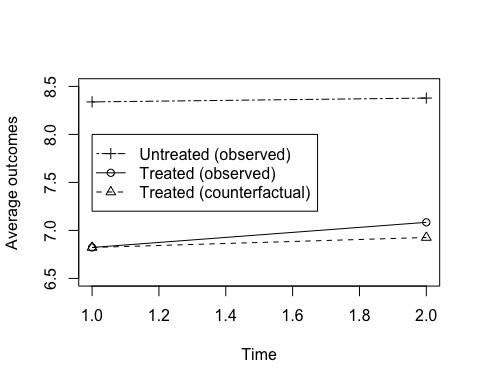
\includegraphics[width=0.6\linewidth]{STCI_files/figure-latex/ploty0y1yBD-1} 

}

\caption{Evolution of average outcomes in the treated and control group before (Time =1) and after (Time=2) the treatment}\label{fig:ploty0y1yBD}
\end{figure}

The estimate of the \(WW\) comparison in the sample is thus:

\begin{align*}
\hat{\Delta^Y_{WW}} & = \frac{1}{\sum_{i=1}^N D_i}\sum_{i=1}^N Y_iD_i-\frac{1}{\sum_{i=1}^N (1-D_i)}\sum_{i=1}^N Y_i(1-D_i).
\end{align*}

We have \(\hat{\Delta^y_{WW}}=\) -1.295. Remember that the value of
\(TT\) in the sample is \(\Delta^y_{TT_s}=\) 0.158.

Overall, \(WW\) severely underestimates the effect of the treatment in
our example. \(WW\) suggests that the treatment has a negative effect on
outcomes whereas we know by construction that it has a positive one.

\subsubsection{Selection bias}\label{selection-bias}

When we form the with/without comparison, we do not recover the \(TT\)
parameter. Instead, we recover \(TT\) plus a bias term, called
\textbf{selection bias}:

\begin{align*}
\Delta^Y_{WW} & =\Delta^Y_{TT}+\Delta^Y_{SB}.
\end{align*}

\BeginKnitrBlock{definition}[Selection bias]
\protect\hypertarget{def:SB}{}{\label{def:SB} \iffalse (Selection bias)
\fi{} }Selection bias is the difference between the with/without
comparison and the treatment on the treated parameter:

\begin{align*}
\Delta^Y_{SB} & = \Delta^Y_{WW}-\Delta^Y_{TT}.
\end{align*}
\EndKnitrBlock{definition}

\(WW\) tries to approximate the counterfactual expected outcome in the
treated group by using \(\esp{Y_i^0|D_i=0}\), the expected outcome in
the untreated group . Selection bias appears because this proxy is
generally poor. It is very easy to see that selection bias is indeed
directly due to this bad proxy problem:

\BeginKnitrBlock{theorem}[Selection bias and counterfactual]
\protect\hypertarget{thm:SBth}{}{\label{thm:SBth} \iffalse (Selection bias
and counterfactual) \fi{} }Selection bias is the difference between the
counterfactual expected potential outcome in the absence of the
treatment among the treated and the expected potential outcome in the
absence of the treatment among the untreated.

\begin{align*}
\Delta^Y_{SB} & = \esp{Y_i^0|D_i=1}-\esp{Y_i^0|D_i=0}.
\end{align*}
\EndKnitrBlock{theorem}

\BeginKnitrBlock{proof}
\iffalse{} {Proof. } \fi{}

\begin{align*}
\Delta^Y_{SB} & = \Delta^Y_{WW}-\Delta^Y_{TT} \\
              & = \esp{Y_i|D_i=1}-\esp{Y_i|D_i=0}-\esp{Y_i^1-Y_i^0|D_i=1}\\
              & = \esp{Y_i^0|D_i=1}-\esp{Y_i^0|D_i=0}.
\end{align*}

The first and second equalities stem only from the definition of both
parameters. The third equality stems from using the switching equation:
\(Y_i=Y_i^1D_i+Y_i^0(1-D_i)\), so that
\(\esp{Y_i|D_i=1}=\esp{Y^1_i|D_i=1}\) and
\(\esp{Y_i|D_i=0}=\esp{Y_i^0|D_i=0}\).
\EndKnitrBlock{proof}

\BeginKnitrBlock{example}
\protect\hypertarget{exm:unnamed-chunk-17}{}{\label{exm:unnamed-chunk-17}
}In the population, \(SB\) is equal to
\EndKnitrBlock{example}

\begin{align*}
  \Delta^y_{SB} & = \Delta^y_{WW}-\Delta^y_{TT} \\
                & = -1.298 - 0.172 \\
                & = -1.471
\end{align*}

We could have computed \(SB\) directly using the formula from Theorem
\ref{thm:SBth}:

\begin{align*}
\Delta^y_{SB} & = \esp{y_i^0|D_i=1}-\esp{y_i^0|D_i=0}\\
              & = -\frac{\sigma^2_{\mu}+\rho\sigma^2_{U}}{\sqrt{\sigma^2_{\mu}+\sigma^2_{U}}}\left(\frac{\phi\left(\frac{\bar{y}-\bar{\mu}}{\sqrt{\sigma^2_{\mu}+\sigma^2_{U}}}\right)}{\Phi\left(\frac{\bar{y}-\bar{\mu}}{\sqrt{\sigma^2_{\mu}+\sigma^2_{U}}}\right)}+\frac{\phi\left(\frac{\bar{y}-\bar{\mu}}{\sqrt{\sigma^2_{\mu}+\sigma^2_{U}}}\right)}{1-\Phi\left(\frac{\bar{y}-\bar{\mu}}{\sqrt{\sigma^2_{\mu}+\sigma^2_{U}}}\right)}\right).
\end{align*}

When using the R function for \(SB\) that we have defined earlier, we
indeed find: \(\Delta^y_{SB}=\) -1.471.

In the sample, \(\hat{\Delta^y_{SB}}=\)-1.295-0.158 \(=\) -1.452.
Selection bias emerges because we are using a bad proxy for the
counterfactual. The average outcome for the untreated is equal to
\(\frac{1}{\sum_{i=1}^N(1-D_i)}\sum_{i=1}^N(1-D_i)y_i=\) 8.378 while the
counterfactual average outcome for the treated is
\(\frac{1}{\sum_{i=1}^ND_i}\sum_{i=1}^ND_iy^0_i=\) 6.926. Their
difference is as expected equal to \(SB\): \(\hat{\Delta^y_{SB}}=\)
6.926 \(-\) 8.378 \(=\) -1.452. The counterfactual average outcome of
the treated is much smaller than the average outcome of the untreated.
On Figure \ref{fig:ploty0y1yBD}, this is materialized by the fact that
the plus sign is located much above the triangle.

\BeginKnitrBlock{remark}
\iffalse{} {Remark. } \fi{}The concept of selection bias is related to
but different from the concept of sample selection bias. With sample
selection bias, we worry that selection into the sample might bias the
estimated effect of a treatment on outcomes. With selection bias, we
worry that selection into the treatment itself might bias the effect of
the treatment on outcomes. Both biases are due to unbserved covariates,
but they do not play out in the same way.

For example, estimating the effect of education on women's wages raises
both selection bias and sample selection bias issues. Selection bias
stems from the fact that more educated women are more likely to be more
dynamic and thus to have higher earnings even when less educated.
Selection bias would be positive in that case, overestimating the effect
of education on earnings.

Sample selection bias stems from the fact that we can only use a sample
of working women in order to estimate the effect of education on wages,
since we do not observe the wages on non working women. But, selection
into the labor force might generate sample selection bias. More educated
women participate more in the labor market, while less educated women
participate less. As a consequence, less educated women that work are
different from the overall sample of less educated women. They might be
more dynamic and work-focused. As a consequence, their wages are higher
than the average wages of the less educated women. Comparing the wages
of less educated women that work to those of more educated women that
work might understate the effect of education on earnings. Sample
selection bias would generate a negative bias on the education
coefficient.
\EndKnitrBlock{remark}

\subsubsection{Confounding factors}\label{confounding-factors}

Confounding factors are the factors that generate differences between
treated and untreated individuals even in the absence of the treatment.
The confounding factors are thus responsible for selection bias. In
general, the mere fact of being selected for receiving the treatment
means that you have a host of characteristics that would differentiate
you from the unselected individuals, even if you were not to receive the
treatment eventually.

For example, if a drug is given to initially sicker individuals, then,
we expect that they will be sicker that the untreated in the absence of
the treatment. Comparing sick individuals to healthy ones is not a sound
way to estimate the effect of a treatment. Obviously, even if our
treatment performs well, healthier individuals will be healthier after
the treatment has been allocated to the sicker patients. The best we can
expect is that the treated patients have recovered, and that their
health after the treatment is comparable to that of the untreated
patients. In that case, the with/without comparison is going to be null,
whereas the true effect of the treatment is positive. Selection bias is
negative in that case: in the absence of the treatment, the average
health status of the treated individuals would have been smaller than
that of the untreated individuals. The confounding factor is the health
status of individuals when the decision to allocate the drug has been
taken. It is correlated to both the allocation of the treatment
(negatively) and to health in the absence of the treatment (positively).

\BeginKnitrBlock{example}
\protect\hypertarget{exm:unnamed-chunk-19}{}{\label{exm:unnamed-chunk-19}
}In our example, \(\mu_i\) and \(U_i^B\) are the confounding factors.
Because the treatment is only given to individuals with pre-treament
outcomes smaller than a threshold (\(y_i^B\leq\bar{y}\)), participants
tend to have smaller \(\mu_i\) and \(U_i^B\) than non participants, as
we can see on Figure \ref{fig:histmuD}.
\EndKnitrBlock{example}

\begin{figure}[htbp]

{\centering 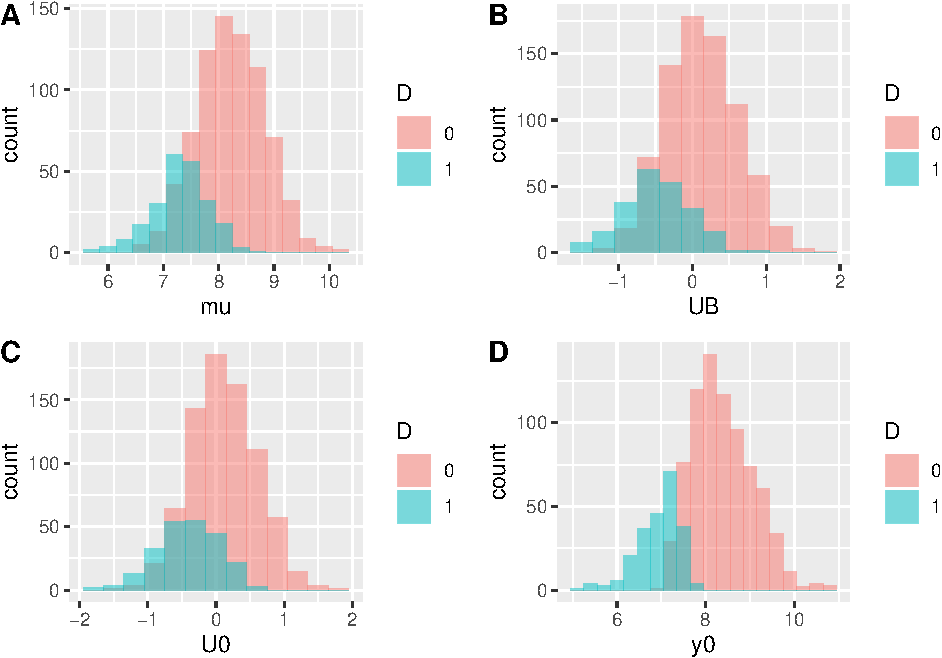
\includegraphics[width=0.6\linewidth]{STCI_files/figure-latex/histmuD-1} 

}

\caption{Distribution of confounders in the treated and control group}\label{fig:histmuD}
\end{figure}

Since confounding factors are persistent, they affect the outcomes of
participants and non participants after the treatment date. \(\mu_i\)
persists entirely over time, and \(U_i^B\) persists at a rate \(\rho\).
As a consequence, even in the absence of the treatment, participants
have lower outcomes than non participants, as we can see on Figure
\ref{fig:histmuD}.

We can derive the contributions of both confouding factors to overall
SB:

\begin{align*}
\esp{Y_i^0|D_i=1} & = \esp{\mu_i+\delta+U_i^0|\mu_i+U_i^B\leq\bar{y}}\\
                  & = \delta + \esp{\mu_i|\mu_i+U_i^B\leq\bar{y}} + \rho\esp{U_i^B|\mu_i+U_i^B\leq\bar{y}}\\
\Delta^y_{SB}     & = \esp{\mu_i|\mu_i+U_i^B\leq\bar{y}}-\esp{\mu_i|\mu_i+U_i^B>\bar{y}} \\
                  & \phantom{=} + \rho\left(\esp{U_i^B|\mu_i+U_i^B\leq\bar{y}}-\esp{U_i^B|\mu_i+U_i^B>\bar{y}}\right)\\
                  & = -\frac{\sigma^2_{\mu}}{\sqrt{\sigma^2_{\mu}+\sigma^2_{U}}}\left(\frac{\phi\left(\frac{\bar{y}-\bar{\mu}}{\sqrt{\sigma^2_{\mu}+\sigma^2_{U}}}\right)}{\Phi\left(\frac{\bar{y}-\bar{\mu}}{\sqrt{\sigma^2_{\mu}+\sigma^2_{U}}}\right)}+\frac{\phi\left(\frac{\bar{y}-\bar{\mu}}{\sqrt{\sigma^2_{\mu}+\sigma^2_{U}}}\right)}{1-\Phi\left(\frac{\bar{y}-\bar{\mu}}{\sqrt{\sigma^2_{\mu}+\sigma^2_{U}}}\right)}\right) \\
                  & \phantom{=} -\frac{\rho\sigma^2_{U}}{\sqrt{\sigma^2_{\mu}+\sigma^2_{U}}}\left(\frac{\phi\left(\frac{\bar{y}-\bar{\mu}}{\sqrt{\sigma^2_{\mu}+\sigma^2_{U}}}\right)}{\Phi\left(\frac{\bar{y}-\bar{\mu}}{\sqrt{\sigma^2_{\mu}+\sigma^2_{U}}}\right)}+\frac{\phi\left(\frac{\bar{y}-\bar{\mu}}{\sqrt{\sigma^2_{\mu}+\sigma^2_{U}}}\right)}{1-\Phi\left(\frac{\bar{y}-\bar{\mu}}{\sqrt{\sigma^2_{\mu}+\sigma^2_{U}}}\right)}\right)
\end{align*}

In order to evaluate these quantities, let's build two R functions:

\begin{Shaded}
\begin{Highlighting}[]
\NormalTok{delta.y.sb.mu <-}\StringTok{ }\ControlFlowTok{function}\NormalTok{(param)\{}
  \KeywordTok{return}\NormalTok{(}\OperatorTok{-}\NormalTok{(param[}\StringTok{"sigma2mu"}\NormalTok{])}\OperatorTok{/}\KeywordTok{sqrt}\NormalTok{(param[}\StringTok{"sigma2mu"}\NormalTok{]}\OperatorTok{+}\NormalTok{param[}\StringTok{"sigma2U"}\NormalTok{])}
         \OperatorTok{*}\KeywordTok{dnorm}\NormalTok{((}\KeywordTok{log}\NormalTok{(param[}\StringTok{"barY"}\NormalTok{])}\OperatorTok{-}\NormalTok{param[}\StringTok{"barmu"}\NormalTok{])}\OperatorTok{/}\NormalTok{(}\KeywordTok{sqrt}\NormalTok{(param[}\StringTok{"sigma2mu"}\NormalTok{]}\OperatorTok{+}\NormalTok{param[}\StringTok{"sigma2U"}\NormalTok{])))}
         \OperatorTok{*}\NormalTok{(}\DecValTok{1}\OperatorTok{/}\KeywordTok{pnorm}\NormalTok{((}\KeywordTok{log}\NormalTok{(param[}\StringTok{"barY"}\NormalTok{])}\OperatorTok{-}\NormalTok{param[}\StringTok{"barmu"}\NormalTok{])}\OperatorTok{/}\NormalTok{(}\KeywordTok{sqrt}\NormalTok{(param[}\StringTok{"sigma2mu"}\NormalTok{]}\OperatorTok{+}\NormalTok{param[}\StringTok{"sigma2U"}\NormalTok{])))}
           \OperatorTok{+}\DecValTok{1}\OperatorTok{/}\NormalTok{(}\DecValTok{1}\OperatorTok{-}\KeywordTok{pnorm}\NormalTok{((}\KeywordTok{log}\NormalTok{(param[}\StringTok{"barY"}\NormalTok{])}\OperatorTok{-}\NormalTok{param[}\StringTok{"barmu"}\NormalTok{])}\OperatorTok{/}\NormalTok{(}\KeywordTok{sqrt}\NormalTok{(param[}\StringTok{"sigma2mu"}\NormalTok{]}\OperatorTok{+}\NormalTok{param[}\StringTok{"sigma2U"}\NormalTok{]))))))}
\NormalTok{\}}
\NormalTok{delta.y.sb.U <-}\StringTok{ }\ControlFlowTok{function}\NormalTok{(param)\{}
  \KeywordTok{return}\NormalTok{(}\OperatorTok{-}\NormalTok{(param[}\StringTok{"rho"}\NormalTok{]}\OperatorTok{*}\NormalTok{param[}\StringTok{"sigma2U"}\NormalTok{])}\OperatorTok{/}\KeywordTok{sqrt}\NormalTok{(param[}\StringTok{"sigma2mu"}\NormalTok{]}\OperatorTok{+}\NormalTok{param[}\StringTok{"sigma2U"}\NormalTok{])}
         \OperatorTok{*}\KeywordTok{dnorm}\NormalTok{((}\KeywordTok{log}\NormalTok{(param[}\StringTok{"barY"}\NormalTok{])}\OperatorTok{-}\NormalTok{param[}\StringTok{"barmu"}\NormalTok{])}\OperatorTok{/}\NormalTok{(}\KeywordTok{sqrt}\NormalTok{(param[}\StringTok{"sigma2mu"}\NormalTok{]}\OperatorTok{+}\NormalTok{param[}\StringTok{"sigma2U"}\NormalTok{])))}
         \OperatorTok{*}\NormalTok{(}\DecValTok{1}\OperatorTok{/}\KeywordTok{pnorm}\NormalTok{((}\KeywordTok{log}\NormalTok{(param[}\StringTok{"barY"}\NormalTok{])}\OperatorTok{-}\NormalTok{param[}\StringTok{"barmu"}\NormalTok{])}\OperatorTok{/}\NormalTok{(}\KeywordTok{sqrt}\NormalTok{(param[}\StringTok{"sigma2mu"}\NormalTok{]}\OperatorTok{+}\NormalTok{param[}\StringTok{"sigma2U"}\NormalTok{])))}
           \OperatorTok{+}\DecValTok{1}\OperatorTok{/}\NormalTok{(}\DecValTok{1}\OperatorTok{-}\KeywordTok{pnorm}\NormalTok{((}\KeywordTok{log}\NormalTok{(param[}\StringTok{"barY"}\NormalTok{])}\OperatorTok{-}\NormalTok{param[}\StringTok{"barmu"}\NormalTok{])}\OperatorTok{/}\NormalTok{(}\KeywordTok{sqrt}\NormalTok{(param[}\StringTok{"sigma2mu"}\NormalTok{]}\OperatorTok{+}\NormalTok{param[}\StringTok{"sigma2U"}\NormalTok{]))))))}
\NormalTok{\}}
\end{Highlighting}
\end{Shaded}

The contribution of \(\mu_i\) to selection bias is -0.978 while that of
\(U_i^0\) is of -0.493.

\subsubsection{\texorpdfstring{When does \(WW\) identify
\(TT\)?}{When does WW identify TT?}}\label{when-does-ww-identify-tt}

Are there conditions under which \(WW\) identify \(TT\)? The answer is
yes: when there is no selection bias, the proxy used by \(WW\) for the
counterfactual quantity is actually valid. Formally, \(WW\) identifies
\(TT\) when the following assumption holds:

\BeginKnitrBlock{definition}[No selection bias]
\protect\hypertarget{def:noselb}{}{\label{def:noselb} \iffalse (No selection
bias) \fi{} }We assume the following:

\begin{align*}
\esp{Y_i^0|D_i=1} & = \esp{Y_i^0|D_i=0}.
\end{align*}
\EndKnitrBlock{definition} Under Assumption \ref{def:noselb}, the
expected counterfactual outcome of the treated is equal to the expected
potential outcome of the untreated in the absence of the treatment. This
yields to the following result:

\BeginKnitrBlock{theorem}
\protect\hypertarget{thm:wwtt}{}{\label{thm:wwtt} }Under Assumption
\ref{def:noselb}, \(WW\) identifies the \(TT\) parameter:

\begin{align*}
\Delta^Y_{WW} & = \Delta^Y_{TT}.
\end{align*}
\EndKnitrBlock{theorem}

\BeginKnitrBlock{proof}
\iffalse{} {Proof. } \fi{}

\begin{align*}
\Delta^Y_{WW} & = \esp{Y_i|D_i=1}-\esp{Y_i|D_i=0}\\
              & = \esp{Y_i^1|D_i=1}-\esp{Y_i^0|D_i=0}\\
              & = \esp{Y_i^1|D_i=1}-\esp{Y_i^0|D_i=1} \\
              & = \Delta^Y_{TT},
\end{align*}

where the second equation uses the switching equation and the third uses
Assumption \ref{def:noselb}.
\EndKnitrBlock{proof}

So, under Assumption \ref{def:noselb}, the \(WW\) comparison actually
identifies the \(TT\) parameter. We say that Assumption \ref{def:noselb}
is an \textbf{identification assumption}: it serves to identify the
parameter of interest using observed data. The intuition for this result
is simply that, under Assumption \ref{def:noselb}, there are no
confounding factors and thus no selection bias. under Assumption
\ref{def:noselb}, the factors that yield individuals to receive or not
the treatment are mean-independent of the potential outcomes in the
absence of the treatment. In this case, the expected outcome in the
untreated group actually is a perfect proxy for the counterfactual
expected outcome of the treated group.

Obviously, Assumption \ref{def:noselb} is extremely unlikely to hold in
real life. For Assumption \ref{def:noselb} to hold, it has to be that
\textbf{all} the determinants of \(D_i\) are actually unrelated to
\(Y_i^0\). One way to enforce Assumption \ref{def:noselb} is to
randomize treatment intake. We will see this in the Lecture on RCTs. It
might also be possible that Assumption \ref{def:noselb} holds in the
data in the absence of an RCT. But this is not very likely, and should
be checked by every mean possible.

One way to test for the validity of Assumption \ref{def:noselb} is to
compare the values of observed covariates in the treated and untreated
group. For Assumption \ref{def:noselb} to be credible, observed
covariates should be distributed in the same way.

Another nice way to test for the validity of Assumption \ref{def:noselb}
with observed data is to implement a \textbf{placebo test}. A placebo
test looks for an effect where there should be none, if we believe the
identification assumptions. For example, under Assumption
\ref{def:noselb} it should be (even though it is not rigorously implied)
that outcomes before the treatment are also mean-independent of the
treatment allocation. And actually, since a future treatment cannot have
an effect today (unless people anticipate the treatment, which we assume
away here), the \(WW\) comparison before the treatment should be null,
therefore giving a zero effect of the placebo treatment ``will receive
the treatment in the future.''

\BeginKnitrBlock{example}
\protect\hypertarget{exm:unnamed-chunk-21}{}{\label{exm:unnamed-chunk-21}
}When the allocation rule defining \(D_i\) is the eligibility rule that
we have used so far, we have already seen that Assumption
\ref{def:noselb} does not hold and the placebo test should not pass
either.
\EndKnitrBlock{example} One way of generating Assumption
\ref{def:noselb} from the eligibility rule that we are using is to mute
the persistence in outcome dynamics. For example, one could set
\(\rho=0\) and \(\sigma^2_{\mu}=0\).

\begin{Shaded}
\begin{Highlighting}[]
\NormalTok{param <-}\StringTok{ }\KeywordTok{c}\NormalTok{(}\DecValTok{8}\NormalTok{,}\DecValTok{0}\NormalTok{,.}\DecValTok{28}\NormalTok{,}\DecValTok{1500}\NormalTok{,}\DecValTok{0}\NormalTok{,}\FloatTok{0.01}\NormalTok{,}\FloatTok{0.05}\NormalTok{,}\FloatTok{0.05}\NormalTok{,}\FloatTok{0.05}\NormalTok{,}\FloatTok{0.1}\NormalTok{)}
\KeywordTok{names}\NormalTok{(param) <-}\StringTok{ }\KeywordTok{c}\NormalTok{(}\StringTok{"barmu"}\NormalTok{,}\StringTok{"sigma2mu"}\NormalTok{,}\StringTok{"sigma2U"}\NormalTok{,}\StringTok{"barY"}\NormalTok{,}\StringTok{"rho"}\NormalTok{,}\StringTok{"theta"}\NormalTok{,}\StringTok{"sigma2epsilon"}\NormalTok{,}\StringTok{"sigma2eta"}\NormalTok{,}\StringTok{"delta"}\NormalTok{,}\StringTok{"baralpha"}\NormalTok{)}
\NormalTok{param}
\end{Highlighting}
\end{Shaded}

\begin{verbatim}
##         barmu      sigma2mu       sigma2U          barY           rho 
##          8.00          0.00          0.28       1500.00          0.00 
##         theta sigma2epsilon     sigma2eta         delta      baralpha 
##          0.01          0.05          0.05          0.05          0.10
\end{verbatim}

In that case, outcomes are not persistent and Assumption
\ref{def:noselb} holds:

\begin{align*}
\esp{y_i^0|D_i=1} & = \esp{\mu_i+\delta+U_i^0|y_i^B\leq\bar{y}}\\
                  & = \esp{\bar{\mu}+\delta+\epsilon_i|\bar{\mu}+U_i^B\leq\bar{y}}\\
                  & = \bar{\mu} + \delta + \esp{\epsilon_i|\bar{\mu}+U_i^B\leq\bar{y}}\\
                  & = \bar{\mu} + \delta + \esp{\epsilon_i|\bar{\mu}+U_i^B>\bar{y}}\\
                  & = \esp{\mu_i+\delta+U_i^0|y_i^B>\bar{y}}\\
                  & = \esp{y_i^0|D_i=0},                  
\end{align*}

where the second equality follows from \(\sigma^2_{\mu}=0\) and
\(\rho=0\) and the fourth from \(\epsilon_i \Ind U_i^B\). Another direct
way to see this is to use the formula for selection bias that we have
derived above. It is easy to see that with \(\rho=0\) and
\(\sigma^2_{\mu}=0\), \(\Delta^y_{SB}=0\). To be sure, we can compute
\(\Delta^y_{SB}\) with the new parameter values: \(\Delta^y_{SB}=\) 0.
As a consequence, \(\Delta^y_{TT}=\) 0.18 \(=\) 0.18 \(=\Delta^y_{WW}\).

\BeginKnitrBlock{remark}
\iffalse{} {Remark. } \fi{}You might have noticed that the value of
\(\Delta^y_{TT}\) is different than before. It is normal, since it
depends on the values of parameters, and especially on
\(\sigma_{\mu}^2\) and \(\rho\).
\EndKnitrBlock{remark}

Let's see how these quantities behave in the sample.

\begin{Shaded}
\begin{Highlighting}[]
\KeywordTok{set.seed}\NormalTok{(}\DecValTok{1234}\NormalTok{)}
\NormalTok{mu <-}\StringTok{ }\KeywordTok{rnorm}\NormalTok{(N,param[}\StringTok{"barmu"}\NormalTok{],}\KeywordTok{sqrt}\NormalTok{(param[}\StringTok{"sigma2mu"}\NormalTok{]))}
\NormalTok{UB <-}\StringTok{ }\KeywordTok{rnorm}\NormalTok{(N,}\DecValTok{0}\NormalTok{,}\KeywordTok{sqrt}\NormalTok{(param[}\StringTok{"sigma2U"}\NormalTok{]))}
\NormalTok{yB <-}\StringTok{ }\NormalTok{mu }\OperatorTok{+}\StringTok{ }\NormalTok{UB }
\NormalTok{YB <-}\StringTok{ }\KeywordTok{exp}\NormalTok{(yB)}
\NormalTok{Ds <-}\StringTok{ }\KeywordTok{rep}\NormalTok{(}\DecValTok{0}\NormalTok{,N)}
\NormalTok{Ds[YB}\OperatorTok{<=}\NormalTok{param[}\StringTok{"barY"}\NormalTok{]] <-}\StringTok{ }\DecValTok{1} 
\NormalTok{epsilon <-}\StringTok{ }\KeywordTok{rnorm}\NormalTok{(N,}\DecValTok{0}\NormalTok{,}\KeywordTok{sqrt}\NormalTok{(param[}\StringTok{"sigma2epsilon"}\NormalTok{]))}
\NormalTok{eta<-}\StringTok{ }\KeywordTok{rnorm}\NormalTok{(N,}\DecValTok{0}\NormalTok{,}\KeywordTok{sqrt}\NormalTok{(param[}\StringTok{"sigma2eta"}\NormalTok{]))}
\NormalTok{U0 <-}\StringTok{ }\NormalTok{param[}\StringTok{"rho"}\NormalTok{]}\OperatorTok{*}\NormalTok{UB }\OperatorTok{+}\StringTok{ }\NormalTok{epsilon}
\NormalTok{y0 <-}\StringTok{ }\NormalTok{mu }\OperatorTok{+}\StringTok{  }\NormalTok{U0 }\OperatorTok{+}\StringTok{ }\NormalTok{param[}\StringTok{"delta"}\NormalTok{]}
\NormalTok{alpha <-}\StringTok{ }\NormalTok{param[}\StringTok{"baralpha"}\NormalTok{]}\OperatorTok{+}\StringTok{  }\NormalTok{param[}\StringTok{"theta"}\NormalTok{]}\OperatorTok{*}\NormalTok{mu }\OperatorTok{+}\StringTok{ }\NormalTok{eta}
\NormalTok{y1 <-}\StringTok{ }\NormalTok{y0}\OperatorTok{+}\NormalTok{alpha}
\NormalTok{Y0 <-}\StringTok{ }\KeywordTok{exp}\NormalTok{(y0)}
\NormalTok{Y1 <-}\StringTok{ }\KeywordTok{exp}\NormalTok{(y1)}
\NormalTok{y <-}\StringTok{ }\NormalTok{y1}\OperatorTok{*}\NormalTok{Ds}\OperatorTok{+}\NormalTok{y0}\OperatorTok{*}\NormalTok{(}\DecValTok{1}\OperatorTok{-}\NormalTok{Ds)}
\NormalTok{Y <-}\StringTok{ }\NormalTok{Y1}\OperatorTok{*}\NormalTok{Ds}\OperatorTok{+}\NormalTok{Y0}\OperatorTok{*}\NormalTok{(}\DecValTok{1}\OperatorTok{-}\NormalTok{Ds)}
\end{Highlighting}
\end{Shaded}

We can see that \(\hat{\esp{Y_i^0|D_i=1}}=\) 8.086 \(\approx\) 8.038
\(=\hat{\esp{Y_i^0|D_i=0}}\). This means that \(WW\) should be close to
\(TT\): \(\hat{\Delta^y_{TT}}=\) 0.16 \(\approx\) 0.208
\(=\hat{\Delta^y_{WW}}\). Note that \(\hat{WW}\) in the sample is not
exactly, but only approximately, equal to \(TT\) in the population and
in the sample. This is an instance of the Fundamental Problem of
Statistical Inference that we will study in the next chapter.

Under these restrictions, the placebo test would unfortunately conclude
against Assumption \ref{def:noselb} even though it is valid:

\begin{align*}
\esp{y_i^B|D_i=1} & = \esp{\mu_i+ U_i^B|y_i^B\leq\bar{y}}\\
                  & = \esp{\bar{\mu}+U_i^B|\bar{\mu}+U_i^B\leq\bar{y}}\\
                  & = \bar{\mu}  + \esp{U_i^B|\bar{\mu}+U_i^B\leq\bar{y}}\\
                  & \neq \bar{\mu}  + \esp{U_i^B|\bar{\mu}+U_i^B>\bar{y}}\\
                  & = \esp{\mu_i+U_i^0|y_i^B>\bar{y}}\\
                  & = \esp{y_i^B|D_i=0}.                  
\end{align*}

In the sample, we indeed have that \(\hat{\esp{Y_i^B|D_i=1}}=\) 7.05
\(\neq\) 8.091 \(=\hat{\esp{Y_i^B|D_i=0}}\). The reason for the failure
of the placebo test to conclude that \(Ww\) is actually correct is that
the \(U_i^B\) shock enters both into the selection equation and the
outcome equation for \(y_i^B\), generating a wage at period \(B\)
between the outcomes of the treated and of the untreated. Since it is
not persistent, this wedge does not generate selection bias. This wedge
would not be detected if we could perform it further back in time,
before the selection period.

Another way to make Assumption \ref{def:noselb} work is to generate a
new allocation rule where all the determinants of treatment intake are
indeed orthogonal to potential outcomes and to outcomes before the
treatment. Let's assume for example that \(D_i=\uns{V_i\leq\bar{y}}\),
with \(V_i\sim\mathcal{N}(\bar{\mu},\sigma^2_{\mu}+\sigma^2_{U})\) and
\(V_i\Ind(Y_i^0,Y_i^1,Y_i^B,\mu_i,\eta_i)\). In that case, Assumption
\ref{def:noselb} holds and the placebo test does work. Indeed, we have:

\begin{align*}
\Delta^y_{TT} & = \esp{Y_i^1-Y_i^0|D_i=1} \\
              & = \esp{\alpha_i|D_i=1} \\
              & = \esp{\bar{\alpha}+\theta\mu_i+\eta_i|V_i\leq\bar{y}}\\
              & = \bar{\alpha}+\theta\bar{\mu} \\
              & = \Delta^y_{ATE} \\
\Delta^y_{WW} & = \esp{Y_i|D_i=1} - \esp{Y_i|D_i=0} \\
              & = \esp{Y^1_i|D_i=1} - \esp{Y^0_i|D_i=0} \\
              & = \esp{Y^1_i|V_i\leq\bar{y}} - \esp{Y^0_i|V_i>\bar{y}} \\
              & = \esp{Y^1_i} - \esp{Y^0_i} \\
              & = \Delta^y_{ATE}
\end{align*}

\(ATE\) is the Average Treatment Effect in the population. It is the
expected effect of the treatment on all the members of the population,
not only on the treated. When the treatment is randomly allocated, both
\(TT\) and \(ATE\) are equal, since the treated are a random subset of
the overall population. I prefer to use \(ATE\) for my definition of the
\(R\) function in order not to erase the definition of the \(TT\)
function:

\begin{Shaded}
\begin{Highlighting}[]
\NormalTok{delta.y.ate <-}\StringTok{ }\ControlFlowTok{function}\NormalTok{(param)\{}
  \KeywordTok{return}\NormalTok{(param[}\StringTok{"baralpha"}\NormalTok{]}\OperatorTok{+}\NormalTok{param[}\StringTok{"theta"}\NormalTok{]}\OperatorTok{*}\NormalTok{param[}\StringTok{"barmu"}\NormalTok{])}
\NormalTok{\}}
\end{Highlighting}
\end{Shaded}

In the population, \(WW\) identifies \(TT\): \(\Delta^y_{TT}=\) 0.18
\(=\Delta^y_{WW}\). Let's see how these quantities behave in the sample:

\begin{Shaded}
\begin{Highlighting}[]
\KeywordTok{set.seed}\NormalTok{(}\DecValTok{1234}\NormalTok{)}
\NormalTok{N <-}\DecValTok{1000}
\NormalTok{mu <-}\StringTok{ }\KeywordTok{rnorm}\NormalTok{(N,param[}\StringTok{"barmu"}\NormalTok{],}\KeywordTok{sqrt}\NormalTok{(param[}\StringTok{"sigma2mu"}\NormalTok{]))}
\NormalTok{UB <-}\StringTok{ }\KeywordTok{rnorm}\NormalTok{(N,}\DecValTok{0}\NormalTok{,}\KeywordTok{sqrt}\NormalTok{(param[}\StringTok{"sigma2U"}\NormalTok{]))}
\NormalTok{yB <-}\StringTok{ }\NormalTok{mu }\OperatorTok{+}\StringTok{ }\NormalTok{UB }
\NormalTok{YB <-}\StringTok{ }\KeywordTok{exp}\NormalTok{(yB)}
\NormalTok{Ds <-}\StringTok{ }\KeywordTok{rep}\NormalTok{(}\DecValTok{0}\NormalTok{,N)}
\NormalTok{V <-}\StringTok{ }\KeywordTok{rnorm}\NormalTok{(N,param[}\StringTok{"barmu"}\NormalTok{],}\KeywordTok{sqrt}\NormalTok{(param[}\StringTok{"sigma2mu"}\NormalTok{]}\OperatorTok{+}\NormalTok{param[}\StringTok{"sigma2U"}\NormalTok{]))}
\NormalTok{Ds[V}\OperatorTok{<=}\KeywordTok{log}\NormalTok{(param[}\StringTok{"barY"}\NormalTok{])] <-}\StringTok{ }\DecValTok{1} 
\NormalTok{epsilon <-}\StringTok{ }\KeywordTok{rnorm}\NormalTok{(N,}\DecValTok{0}\NormalTok{,}\KeywordTok{sqrt}\NormalTok{(param[}\StringTok{"sigma2epsilon"}\NormalTok{]))}
\NormalTok{eta<-}\StringTok{ }\KeywordTok{rnorm}\NormalTok{(N,}\DecValTok{0}\NormalTok{,}\KeywordTok{sqrt}\NormalTok{(param[}\StringTok{"sigma2eta"}\NormalTok{]))}
\NormalTok{U0 <-}\StringTok{ }\NormalTok{param[}\StringTok{"rho"}\NormalTok{]}\OperatorTok{*}\NormalTok{UB }\OperatorTok{+}\StringTok{ }\NormalTok{epsilon}
\NormalTok{y0 <-}\StringTok{ }\NormalTok{mu }\OperatorTok{+}\StringTok{  }\NormalTok{U0 }\OperatorTok{+}\StringTok{ }\NormalTok{param[}\StringTok{"delta"}\NormalTok{]}
\NormalTok{alpha <-}\StringTok{ }\NormalTok{param[}\StringTok{"baralpha"}\NormalTok{]}\OperatorTok{+}\StringTok{  }\NormalTok{param[}\StringTok{"theta"}\NormalTok{]}\OperatorTok{*}\NormalTok{mu }\OperatorTok{+}\StringTok{ }\NormalTok{eta}
\NormalTok{y1 <-}\StringTok{ }\NormalTok{y0}\OperatorTok{+}\NormalTok{alpha}
\NormalTok{Y0 <-}\StringTok{ }\KeywordTok{exp}\NormalTok{(y0)}
\NormalTok{Y1 <-}\StringTok{ }\KeywordTok{exp}\NormalTok{(y1)}
\NormalTok{y <-}\StringTok{ }\NormalTok{y1}\OperatorTok{*}\NormalTok{Ds}\OperatorTok{+}\NormalTok{y0}\OperatorTok{*}\NormalTok{(}\DecValTok{1}\OperatorTok{-}\NormalTok{Ds)}
\NormalTok{Y <-}\StringTok{ }\NormalTok{Y1}\OperatorTok{*}\NormalTok{Ds}\OperatorTok{+}\NormalTok{Y0}\OperatorTok{*}\NormalTok{(}\DecValTok{1}\OperatorTok{-}\NormalTok{Ds)}
\end{Highlighting}
\end{Shaded}

In the sample, the counterfactual is well approximated by the outcomes
of the untreated: \(\hat{\esp{Y_i^0|D_i=1}}=\) 8.038 \(\approx\) 8.055
\(=\hat{\esp{Y_i^0|D_i=0}}\). As a consequence, \(WW\) should be close
to \(TT\): \(\hat{\Delta^y_{TT}}=\) 0.183 \(\approx\) 0.167
\(=\hat{\Delta^y_{WW}}\). The placebo test is also valid in that case:
\(\hat{\esp{Y_i^B|D_i=1}}=\) 7.922 \(\approx\) 8.016
\(=\hat{\esp{Y_i^B|D_i=0}}\).

\subsection{The before/after comparison, temporal confounders and time
trend
bias}\label{the-beforeafter-comparison-temporal-confounders-and-time-trend-bias}

The before/after comparison (\(BA\)) is also very intuitive: it consists
in looking at how the outcomes of the treated have changed over time and
to attribute this change to the effect of the treatment. The problem is
that other changes might have affected outcomes in the absence of the
treatment, thereby biasing \(BA\). The bias of \(BA\) is called
time-trend bias. It is due to confounders that affect the outcomes of
the treated over time. This section defines the \(BA\) estimator,
derives its bias, describes the role of the confounders and states
conditions under which \(BA\) identifies \(TT\).

\BeginKnitrBlock{example}
\protect\hypertarget{exm:unnamed-chunk-23}{}{\label{exm:unnamed-chunk-23}
}Before computing any estimates, we need to reset all our parameter
values and generated sample it their usual values:
\EndKnitrBlock{example}

\begin{Shaded}
\begin{Highlighting}[]
\NormalTok{param <-}\StringTok{ }\KeywordTok{c}\NormalTok{(}\DecValTok{8}\NormalTok{,.}\DecValTok{5}\NormalTok{,.}\DecValTok{28}\NormalTok{,}\DecValTok{1500}\NormalTok{)}
\KeywordTok{names}\NormalTok{(param) <-}\StringTok{ }\KeywordTok{c}\NormalTok{(}\StringTok{"barmu"}\NormalTok{,}\StringTok{"sigma2mu"}\NormalTok{,}\StringTok{"sigma2U"}\NormalTok{,}\StringTok{"barY"}\NormalTok{)}
\KeywordTok{set.seed}\NormalTok{(}\DecValTok{1234}\NormalTok{)}
\NormalTok{N <-}\DecValTok{1000}
\NormalTok{mu <-}\StringTok{ }\KeywordTok{rnorm}\NormalTok{(N,param[}\StringTok{"barmu"}\NormalTok{],}\KeywordTok{sqrt}\NormalTok{(param[}\StringTok{"sigma2mu"}\NormalTok{]))}
\NormalTok{UB <-}\StringTok{ }\KeywordTok{rnorm}\NormalTok{(N,}\DecValTok{0}\NormalTok{,}\KeywordTok{sqrt}\NormalTok{(param[}\StringTok{"sigma2U"}\NormalTok{]))}
\NormalTok{yB <-}\StringTok{ }\NormalTok{mu }\OperatorTok{+}\StringTok{ }\NormalTok{UB }
\NormalTok{YB <-}\StringTok{ }\KeywordTok{exp}\NormalTok{(yB)}
\NormalTok{Ds <-}\StringTok{ }\KeywordTok{rep}\NormalTok{(}\DecValTok{0}\NormalTok{,N)}
\NormalTok{Ds[YB}\OperatorTok{<=}\NormalTok{param[}\StringTok{"barY"}\NormalTok{]] <-}\StringTok{ }\DecValTok{1} 
\NormalTok{l <-}\StringTok{ }\KeywordTok{length}\NormalTok{(param)}
\NormalTok{param <-}\StringTok{ }\KeywordTok{c}\NormalTok{(param,}\FloatTok{0.9}\NormalTok{,}\FloatTok{0.01}\NormalTok{,}\FloatTok{0.05}\NormalTok{,}\FloatTok{0.05}\NormalTok{,}\FloatTok{0.05}\NormalTok{,}\FloatTok{0.1}\NormalTok{)}
\KeywordTok{names}\NormalTok{(param)[(l}\OperatorTok{+}\DecValTok{1}\NormalTok{)}\OperatorTok{:}\KeywordTok{length}\NormalTok{(param)] <-}\StringTok{ }\KeywordTok{c}\NormalTok{(}\StringTok{"rho"}\NormalTok{,}\StringTok{"theta"}\NormalTok{,}\StringTok{"sigma2epsilon"}\NormalTok{,}\StringTok{"sigma2eta"}\NormalTok{,}\StringTok{"delta"}\NormalTok{,}\StringTok{"baralpha"}\NormalTok{)}
\NormalTok{epsilon <-}\StringTok{ }\KeywordTok{rnorm}\NormalTok{(N,}\DecValTok{0}\NormalTok{,}\KeywordTok{sqrt}\NormalTok{(param[}\StringTok{"sigma2epsilon"}\NormalTok{]))}
\NormalTok{eta<-}\StringTok{ }\KeywordTok{rnorm}\NormalTok{(N,}\DecValTok{0}\NormalTok{,}\KeywordTok{sqrt}\NormalTok{(param[}\StringTok{"sigma2eta"}\NormalTok{]))}
\NormalTok{U0 <-}\StringTok{ }\NormalTok{param[}\StringTok{"rho"}\NormalTok{]}\OperatorTok{*}\NormalTok{UB }\OperatorTok{+}\StringTok{ }\NormalTok{epsilon}
\NormalTok{y0 <-}\StringTok{ }\NormalTok{mu }\OperatorTok{+}\StringTok{  }\NormalTok{U0 }\OperatorTok{+}\StringTok{ }\NormalTok{param[}\StringTok{"delta"}\NormalTok{]}
\NormalTok{alpha <-}\StringTok{ }\NormalTok{param[}\StringTok{"baralpha"}\NormalTok{]}\OperatorTok{+}\StringTok{  }\NormalTok{param[}\StringTok{"theta"}\NormalTok{]}\OperatorTok{*}\NormalTok{mu }\OperatorTok{+}\StringTok{ }\NormalTok{eta}
\NormalTok{y1 <-}\StringTok{ }\NormalTok{y0}\OperatorTok{+}\NormalTok{alpha}
\NormalTok{Y0 <-}\StringTok{ }\KeywordTok{exp}\NormalTok{(y0)}
\NormalTok{Y1 <-}\StringTok{ }\KeywordTok{exp}\NormalTok{(y1)}
\NormalTok{y <-}\StringTok{ }\NormalTok{y1}\OperatorTok{*}\NormalTok{Ds}\OperatorTok{+}\NormalTok{y0}\OperatorTok{*}\NormalTok{(}\DecValTok{1}\OperatorTok{-}\NormalTok{Ds)}
\NormalTok{Y <-}\StringTok{ }\NormalTok{Y1}\OperatorTok{*}\NormalTok{Ds}\OperatorTok{+}\NormalTok{Y0}\OperatorTok{*}\NormalTok{(}\DecValTok{1}\OperatorTok{-}\NormalTok{Ds)}
\end{Highlighting}
\end{Shaded}

\subsubsection{The before/after
comparison}\label{the-beforeafter-comparison}

The before/after estimator (\(BA\)) compares the outcomes of the treated
after taking the treatment to the outcomes of the treated before taking
the treatment. It is also sometimes called a ``pre-post comparison.''

\BeginKnitrBlock{definition}[Before/after comparison]
\protect\hypertarget{def:unnamed-chunk-24}{}{\label{def:unnamed-chunk-24}
\iffalse (Before/after comparison) \fi{} }The before/after comparison is
the difference between the expected outcomes in the treated group after
the treatment and the expected outcomes in the same group before the
treatment:

\begin{align*}
\Delta^Y_{BA} & =  \esp{Y_i|D_i=1}-\esp{Y^B_i|D_i=1}.
\end{align*}
\EndKnitrBlock{definition}

\BeginKnitrBlock{example}
\protect\hypertarget{exm:unnamed-chunk-25}{}{\label{exm:unnamed-chunk-25}
}In the population, the \(BA\) estimator has the following shape:

\begin{align*}
  \Delta^y_{BA} & = \esp{y_i|D_i=1}-\esp{y^B_i|D_i=1}\\
                & = \esp{y^1_i-y^B_i|D_i=1}\\
                & = \esp{\alpha_i|D_i=1} + \delta + (\rho-1)\esp{U_i^B|\mu_i+U_i^B\leq\bar{y}}\\
                & = \Delta^y_{TT} + \delta + (1-\rho)\left(\frac{\sigma^2_{U}}{\sqrt{\sigma^2_{\mu}+\sigma^2_{U}}}\frac{\phi\left(\frac{\bar{y}-\bar{\mu}}{\sqrt{\sigma^2_{\mu}+\sigma^2_{U}}}\right)}{\Phi\left(\frac{\bar{y}-\bar{\mu}}{\sqrt{\sigma^2_{\mu}+\sigma^2_{U}}}\right)}\right).
\end{align*}
\EndKnitrBlock{example}

In order to compute \(BA\) in the population, we can again use a R
function, combining the value of \(TT\) and that of the second part of
the formula, that we are going to denote \(TB\) for reasons that are
going to become clear in a bit.

\begin{Shaded}
\begin{Highlighting}[]
\NormalTok{delta.y.tb <-}\StringTok{ }\ControlFlowTok{function}\NormalTok{(param)\{}
  \KeywordTok{return}\NormalTok{(param[}\StringTok{"delta"}\NormalTok{]}
          \OperatorTok{+}\NormalTok{(}\DecValTok{1}\OperatorTok{-}\NormalTok{param[}\StringTok{"rho"}\NormalTok{])}\OperatorTok{*}\NormalTok{((param[}\StringTok{"sigma2U"}\NormalTok{])}\OperatorTok{/}\KeywordTok{sqrt}\NormalTok{(param[}\StringTok{"sigma2mu"}\NormalTok{]}\OperatorTok{+}\NormalTok{param[}\StringTok{"sigma2U"}\NormalTok{]))}
         \OperatorTok{*}\KeywordTok{dnorm}\NormalTok{((}\KeywordTok{log}\NormalTok{(param[}\StringTok{"barY"}\NormalTok{])}\OperatorTok{-}\NormalTok{param[}\StringTok{"barmu"}\NormalTok{])}\OperatorTok{/}\NormalTok{(}\KeywordTok{sqrt}\NormalTok{(param[}\StringTok{"sigma2mu"}\NormalTok{]}\OperatorTok{+}\NormalTok{param[}\StringTok{"sigma2U"}\NormalTok{])))}
         \OperatorTok{/}\KeywordTok{pnorm}\NormalTok{((}\KeywordTok{log}\NormalTok{(param[}\StringTok{"barY"}\NormalTok{])}\OperatorTok{-}\NormalTok{param[}\StringTok{"barmu"}\NormalTok{])}\OperatorTok{/}\NormalTok{(}\KeywordTok{sqrt}\NormalTok{(param[}\StringTok{"sigma2mu"}\NormalTok{]}\OperatorTok{+}\NormalTok{param[}\StringTok{"sigma2U"}\NormalTok{]))))}
\NormalTok{\}}
\NormalTok{delta.y.ba <-}\StringTok{ }\ControlFlowTok{function}\NormalTok{(param)\{}
  \KeywordTok{return}\NormalTok{(}\KeywordTok{delta.y.tt}\NormalTok{(param)}\OperatorTok{+}\StringTok{ }\KeywordTok{delta.y.tb}\NormalTok{(param))}
\NormalTok{\}}
\end{Highlighting}
\end{Shaded}

The value of \(BA\) in the population is thus \(\Delta^y_{BA}=\) 0.265.
Remember that the true value of \(TT\) in the population is 0.172. In
the sample, the value of \(BA\) is \(\hat{\Delta^y_{BA}}=\) 0.262.
Remember that the value of \(TT\) in the sample is \(\Delta^y_{TT_s}=\)
0.158.

\subsubsection{Time trend bias}\label{time-trend-bias}

When we form the before/after comparison, we do not recover the \(TT\)
parameter. Instead, we recover \(TT\) plus a bias term, called
\textbf{time trend bias}:

\begin{align*}
\Delta^Y_{BA} & =\Delta^Y_{TT}+\Delta^Y_{TB}.
\end{align*}

\BeginKnitrBlock{definition}[Time trend bias]
\protect\hypertarget{def:unnamed-chunk-26}{}{\label{def:unnamed-chunk-26}
\iffalse (Time trend bias) \fi{} }Time trend bias is the difference
between the before/after comparison and the treatment on the treated
parameter:

\begin{align*}
\Delta^Y_{TB} & = \Delta^Y_{BA}-\Delta^Y_{TT} .
\end{align*}
\EndKnitrBlock{definition}

\(BA\) uses the expected outcome in the treated group before the
treatment as a proxy for the expected counterfactual outcome in the
absence of the treatment in the same group. \(TB\) is due to the fact
that \(BA\) uses an imperfect proxy for the counterfactual expected
outcome of the treated:

\BeginKnitrBlock{theorem}
\protect\hypertarget{thm:TB}{}{\label{thm:TB} }Time trend bias is the
difference between the counterfactual expected potential outcome in the
absence of the treatment among the treated and the expected outcome
before the treatment in the same group.

\begin{align*}
\Delta^Y_{TB} & = \esp{Y_i^0|D_i=1}-\esp{Y_i^B|D_i=1}.
\end{align*}
\EndKnitrBlock{theorem}

\BeginKnitrBlock{proof}
\iffalse{} {Proof. } \fi{}

\begin{align*}
\Delta^Y_{TB} & = \Delta^Y_{BA}-\Delta^Y_{TT} \\
              & = \esp{Y_i|D_i=1}-\esp{Y^B_i|D_i=1}-\esp{Y_i^1-Y_i^0|D_i=1}\\
              & = \esp{Y_i^0|D_i=1}-\esp{Y_i^B|D_i=1}.
\end{align*}

The first and second equalities stem from the definition of both
parameters. The third equality stems from using the switching equation:
\(Y_i=Y_i^1D_i+Y_i^0(1-D_i)\), so that
\(\esp{Y_i|D_i=1}=\esp{Y^1_i|D_i=1}\).
\EndKnitrBlock{proof}

\BeginKnitrBlock{example}
\protect\hypertarget{exm:unnamed-chunk-28}{}{\label{exm:unnamed-chunk-28}
}In the population, \(TB\) is equal to
\EndKnitrBlock{example} \(\Delta^y_{TB}=\Delta^y_{BA}-\Delta^y_{TT}=\)
0.265 \(-\) 0.172 \(=\) 0.093. We could have computed this result using
Theorem\ref{thm:TB}:

\begin{align*}
\Delta^y_{TB} & = \esp{y_i^0|D_i=1}-\esp{y_i^B|D_i=1} \\
              & = \delta + (1-\rho)\left(\frac{\sigma^2_{U}}{\sqrt{\sigma^2_{\mu}+\sigma^2_{U}}}\frac{\phi\left(\frac{\bar{y}-\bar{\mu}}{\sqrt{\sigma^2_{\mu}+\sigma^2_{U}}}\right)}{\Phi\left(\frac{\bar{y}-\bar{\mu}}{\sqrt{\sigma^2_{\mu}+\sigma^2_{U}}}\right)}\right).
\end{align*}

Using the R function that we have defined previously, this approach
gives \(\Delta^y_{TB}=\) 0.093.

In the sample \(\hat{\Delta^y_{BA}}=\) 0.262 while
\(\hat{\Delta^y_{TT}}=\) 0.158, so that \(\hat{\Delta^y_{TB}}=\) 0.104.
Time trend bias emerges because we are using a bad proxy for the
counterfactual average outcomes of the treated. The average outcome of
the treated before the treatment takes place is
\(\hat{\esp{y_i^B|D_i=1}}=\) 6.822 while the true counterfactual average
outcome for the treated after the treatment is
\(\hat{\esp{y_i^0|D_i=1}}=\) 6.926. Outcomes would have increased in the
treatment group even in the absence of the treatment. As a consequence,
the \(BA\) comparison overestimates the true effect of the treatment.
\(TB\) estimated using Theorem \ref{thm:TB} is equal to:
\(\hat{\Delta^y_{TB}}=\) 6.926 \(-\) 6.822 \(=\) 0.104. This can be seen
on Figure \ref{fig:ploty0y1yBD}: the triangle in period 2 is higher than
in period 1.

\subsubsection{Temporal confounders}\label{temporal-confounders}

Temporal confounders make the outcomes of the treated change at the same
time as the treatment status changes, thereby confounding the effect of
the treatment. Temporal confounders are responsible for time trend bias.

Over time, there are other things that change than the treatment status.
For example, maybe sick individuals naturally recover, and thus their
counterfactual health status is better than ther health status before
taking the treatment. As a results, \(BA\) might overstimate the effect
of the treatment. It might also be that the overall level of health in
the country has increased, because of increasing GDP, for example.

\BeginKnitrBlock{example}
\protect\hypertarget{exm:unnamed-chunk-29}{}{\label{exm:unnamed-chunk-29}
}In our example, \(\delta\) and \(U_i^B\) are the confounders.
\(\delta\) captures the overall changes in outcomes over time (business
cycle, general improvement of health status). \(U^B_i\) captures the
fact that transitorily sicker individuals tend at the same time to
receive the treatment and also to recover naturally. The \(BA\)
comparison incorrectly attributes both of these changes to the effect of
the treatment. We can compute the relative contributions of both sources
to the overall time-trend bias in the population.
\EndKnitrBlock{example} \(\delta\) contributes for 0.05 while \(U^B_i\)
contributes for 0.043.

\subsubsection{\texorpdfstring{When does \(BA\) identify
\(TT\)?}{When does BA identify TT?}}\label{when-does-ba-identify-tt}

Are there conditions under which \(BA\) actually identifies \(TT\)? The
answer is yes, when there are no temporal confounders. When that is the
case, the variation of outcomes over time is only due to the treatment
and it identifies the treatment effect.

More formally, we make the following assumption:

\BeginKnitrBlock{definition}[No time trend bias]
\protect\hypertarget{def:notb}{}{\label{def:notb} \iffalse (No time trend
bias) \fi{} }We assume the following:

\begin{align*}
\esp{Y_i^0|D_i=1} & = \esp{Y_i^B|D_i=1}.
\end{align*}
\EndKnitrBlock{definition}

Under Assumption \ref{def:notb}, the expected counterfactual outcome of
the treated is equal to the expected potential outcome of the untreated
in the absence of the treatment. This yields to the following result:

\BeginKnitrBlock{theorem}
\protect\hypertarget{thm:batt}{}{\label{thm:batt} }Under Assumption
\ref{def:notb}, \(BA\) identifies the \(TT\) parameter:

\begin{align*}
\Delta^Y_{BA} & = \Delta^Y_{TT}.
\end{align*}
\EndKnitrBlock{theorem}

\BeginKnitrBlock{proof}
\iffalse{} {Proof. } \fi{}

\begin{align*}
\Delta^Y_{BA} & = \esp{Y_i|D_i=1}-\esp{Y_i^B|D_i=1}\\
              & = \esp{Y_i^1|D_i=1}-\esp{Y_i^B|D_i=1}\\
              & = \esp{Y_i^1|D_i=1}-\esp{Y_i^0|D_i=1} \\
              & = \Delta^Y_{TT},
\end{align*}

where the second equation uses the switching equation and the third uses
Assumption \ref{def:notb}.
\EndKnitrBlock{proof}

Under Assumption \ref{def:notb} the outcomes of the treated before the
treatment takes place are a good proxy for the counterfactual. As a
consequence, \(BA\) identifies \(TT\). Under Assumption \ref{def:notb}is
very unlikely to hold in real life. Indeed, it requires tha nothing
happens to the outcomes of the treated in the absence of the treatment.
Assumption \ref{def:notb} rules out economy-wide shocks but also
mean-reversion, such as when sick people naturally recover from an
illness.

A good way to test for the validity of Assumption \ref{def:notb} is to
perform a placebo test. Two of these tests are possible. One placebo
test would be to apply the \(BA\) estimator between two pre-treatment
periods where nothing should happen since the treatment status does not
vary and, by assumption, nothing else should vary. A second placebo test
would be to apply the \(BA\) estimator to a group that does not receive
the treatment. The untreated group is a perfectly suitable candidate for
that. Assumption \ref{def:notb} does not imply that there should be no
change in the untreated outcomes, but detecting such a change would cast
a serious doubt on the validity of Assumption \ref{def:notb}.

\BeginKnitrBlock{example}
\protect\hypertarget{exm:unnamed-chunk-31}{}{\label{exm:unnamed-chunk-31}
}One way to generate a population in which Assumption \ref{def:notb}
holds is to shut down the two sources of confounders in our original
model by setting both \(\delta=0\) and \(\rho=1\).
\EndKnitrBlock{example}

\begin{Shaded}
\begin{Highlighting}[]
\NormalTok{param <-}\StringTok{ }\KeywordTok{c}\NormalTok{(}\DecValTok{8}\NormalTok{,}\FloatTok{0.5}\NormalTok{,.}\DecValTok{28}\NormalTok{,}\DecValTok{1500}\NormalTok{,}\DecValTok{1}\NormalTok{,}\FloatTok{0.01}\NormalTok{,}\FloatTok{0.05}\NormalTok{,}\FloatTok{0.05}\NormalTok{,}\DecValTok{0}\NormalTok{,}\FloatTok{0.1}\NormalTok{)}
\KeywordTok{names}\NormalTok{(param) <-}\StringTok{ }\KeywordTok{c}\NormalTok{(}\StringTok{"barmu"}\NormalTok{,}\StringTok{"sigma2mu"}\NormalTok{,}\StringTok{"sigma2U"}\NormalTok{,}\StringTok{"barY"}\NormalTok{,}\StringTok{"rho"}\NormalTok{,}\StringTok{"theta"}\NormalTok{,}\StringTok{"sigma2epsilon"}\NormalTok{,}\StringTok{"sigma2eta"}\NormalTok{,}\StringTok{"delta"}\NormalTok{,}\StringTok{"baralpha"}\NormalTok{)}
\NormalTok{param}
\end{Highlighting}
\end{Shaded}

\begin{verbatim}
##         barmu      sigma2mu       sigma2U          barY           rho 
##          8.00          0.50          0.28       1500.00          1.00 
##         theta sigma2epsilon     sigma2eta         delta      baralpha 
##          0.01          0.05          0.05          0.00          0.10
\end{verbatim}

In that case, according to the formula we have derived for \(TB\), we
have: \(\Delta^y_{TB}=\) 0. Let's see how these quantities behave in the
sample:

\begin{Shaded}
\begin{Highlighting}[]
\KeywordTok{set.seed}\NormalTok{(}\DecValTok{1234}\NormalTok{)}
\NormalTok{mu <-}\StringTok{ }\KeywordTok{rnorm}\NormalTok{(N,param[}\StringTok{"barmu"}\NormalTok{],}\KeywordTok{sqrt}\NormalTok{(param[}\StringTok{"sigma2mu"}\NormalTok{]))}
\NormalTok{UB <-}\StringTok{ }\KeywordTok{rnorm}\NormalTok{(N,}\DecValTok{0}\NormalTok{,}\KeywordTok{sqrt}\NormalTok{(param[}\StringTok{"sigma2U"}\NormalTok{]))}
\NormalTok{yB <-}\StringTok{ }\NormalTok{mu }\OperatorTok{+}\StringTok{ }\NormalTok{UB }
\NormalTok{YB <-}\StringTok{ }\KeywordTok{exp}\NormalTok{(yB)}
\NormalTok{Ds <-}\StringTok{ }\KeywordTok{rep}\NormalTok{(}\DecValTok{0}\NormalTok{,N)}
\NormalTok{Ds[YB}\OperatorTok{<=}\NormalTok{param[}\StringTok{"barY"}\NormalTok{]] <-}\StringTok{ }\DecValTok{1} 
\NormalTok{epsilon <-}\StringTok{ }\KeywordTok{rnorm}\NormalTok{(N,}\DecValTok{0}\NormalTok{,}\KeywordTok{sqrt}\NormalTok{(param[}\StringTok{"sigma2epsilon"}\NormalTok{]))}
\NormalTok{eta<-}\StringTok{ }\KeywordTok{rnorm}\NormalTok{(N,}\DecValTok{0}\NormalTok{,}\KeywordTok{sqrt}\NormalTok{(param[}\StringTok{"sigma2eta"}\NormalTok{]))}
\NormalTok{U0 <-}\StringTok{ }\NormalTok{param[}\StringTok{"rho"}\NormalTok{]}\OperatorTok{*}\NormalTok{UB }\OperatorTok{+}\StringTok{ }\NormalTok{epsilon}
\NormalTok{y0 <-}\StringTok{ }\NormalTok{mu }\OperatorTok{+}\StringTok{  }\NormalTok{U0 }\OperatorTok{+}\StringTok{ }\NormalTok{param[}\StringTok{"delta"}\NormalTok{]}
\NormalTok{alpha <-}\StringTok{ }\NormalTok{param[}\StringTok{"baralpha"}\NormalTok{]}\OperatorTok{+}\StringTok{  }\NormalTok{param[}\StringTok{"theta"}\NormalTok{]}\OperatorTok{*}\NormalTok{mu }\OperatorTok{+}\StringTok{ }\NormalTok{eta}
\NormalTok{y1 <-}\StringTok{ }\NormalTok{y0}\OperatorTok{+}\NormalTok{alpha}
\NormalTok{Y0 <-}\StringTok{ }\KeywordTok{exp}\NormalTok{(y0)}
\NormalTok{Y1 <-}\StringTok{ }\KeywordTok{exp}\NormalTok{(y1)}
\NormalTok{y <-}\StringTok{ }\NormalTok{y1}\OperatorTok{*}\NormalTok{Ds}\OperatorTok{+}\NormalTok{y0}\OperatorTok{*}\NormalTok{(}\DecValTok{1}\OperatorTok{-}\NormalTok{Ds)}
\NormalTok{Y <-}\StringTok{ }\NormalTok{Y1}\OperatorTok{*}\NormalTok{Ds}\OperatorTok{+}\NormalTok{Y0}\OperatorTok{*}\NormalTok{(}\DecValTok{1}\OperatorTok{-}\NormalTok{Ds)}
\end{Highlighting}
\end{Shaded}

In the sample, the value of \(BA\) is \(\hat{\Delta^y_{BA}}=\) 0.164
while the value of \(TT\) in the sample is \(\Delta^y_{TT_s}=\) 0.158.
We cannot perform a placebo test using two periods of pre-treatment
outcomes for the treated since we have generated only one period of
pre-treatment outcome. We will be able to perform this test later in the
DID lecture. We can perfom the placebo test that applies the \(BA\)
estimator to the untreated. The value of \(BA\) for the untreated is
\(\hat{\Delta^y_{BA|D=0}}=\) 0.002, which is reasonably close to zero.

\chapter{Fundamental Problem of Statistical Inference}\label{FPSI}

The Fundamental Problem of Statistical Inference (FPSI) states that,
even if we have an estimator \(E\) that identifies \(TT\) in the
population, we cannot observe \(E\) because we only have access to a
finite sample of the population. The only thing that we can form from
the sample is a sample equivalent \(\hat{E}\) to the population quantity
\(E\), and \(\hat{E}\neq E\). For example, the sample analog to \(WW\)
is the difference in means between treated and untreated units
\(\hat{WW}\). As we saw in the last lecture, \(\hat{WW}\) is never
exactly equal to \(WW\).

Why is \(\hat{E}\neq E\)? Because a finite sample is never perfectly
representative of the population. In a sample, even in a random sample,
the distribution of the observed and unobserved covariates deviates from
the true population one. As a consequence, the sample value of the
estimator is never precisely equal to the population value, but
fluctuates around it with sampling noise. The main problem with the FPSI
is that if we find an effect of our treatment, be it small or large, we
cannot know whether we should attribute it to the treatment or to the
bad or good luck of sampling noise.

What can we do to deal with the FPSI? I am going to argue that there are
mainly two things that we might want to do: estimating the extent of
sampling noise and decreasing sampling noise.

Estimating sampling noise means measuring how much variability there is
in our estimate \(\hat{E}\) due to the sampling procedure. This is very
useful because it enables us to form a confidence interval that gauges
how far from \(\hat{E}\) the true value \(E\) might be. It is a measure
of the precision of our estimation and of the extent to which sampling
noise might drive our results. Estimating sampling noise is very hard
because we have only access to one sample and we would like to know the
behavior of our estimator over repeated samples. We are going to learn
four ways to estimate the extent of sampling noise using data from one
sample.

Because sampling noise is such a nuisance and makes our estimates
imprecise, we would like to be able to make it as small as possible. We
are going to study three ways of decreasing sampling noise, two that
take place before collecting the data (increasing sample size,
stratifying) and one that takes place after (conditioning).

Maybe you are surprised not to find statistical significance tests as an
important answer to the FPSI. I argue in this lecture that statistical
tests are misleading tools that make us overestimate the confidence in
our results and underestimate the scope of sampling noise. Statistical
tests are not meant to be used for scientific research, but were
originally designed to make decisions in industrial settings where the
concept of successive sampling made actual sense. Statistical tests also
generate collective behaviors such as publication bias and specification
search that undermine the very foundations of science. A general
movement in the social sciences, but also in physics, is starting to ban
the reporting of p-values.

\section{What is sampling noise? Definition and
illustration}\label{sec:sampnoise}

In this section, I am going to define sampling noise and illustrate it
with a numerical example. In Section \ref{sec:definitionnoise}, I define
sampling noise. In section \ref{sec:illusnoisepop}, I illustrate how
sampling noise varies when one is interested in the population treatment
effect. In section \ref{sec:illusnoisesamp}, I illustrate how sampling
noise varies when one is interesetd in the sample treatment effect.
Finally, in section \ref{sec:confinterv}, I show how confidence
intervals can be built from an estimate of sampling noise.

\subsection{Sampling noise, a definition}\label{sec:definitionnoise}

Sampling noise measures how much sampling variability moves the sample
estimator \(\hat{E}\) around. One way to define it more rigorously is to
make it equal to the width of a confidence interval:

\BeginKnitrBlock{definition}[Sampling noise]
\protect\hypertarget{def:sampnoise}{}{\label{def:sampnoise}
\iffalse (Sampling noise) \fi{} }Sampling noise is the width of the
symmetric interval around TT within which \(\delta*100\)\% of the sample
estimators fall, where \(\delta\) is the confidence level. As a
consequence, sampling noise is equal to \(2\epsilon\) where \(\epsilon\)
is such that:

\begin{align*}
\Pr(|\hat{E}-TT|\leq\epsilon) &= \delta.
\end{align*}
\EndKnitrBlock{definition}

This definition tries to capture the properties of the distribution of
\(\hat{E}\) using only one number. As every simplification, it leaves
room for dissatisfaction, exactly as a 2D map is a convenient albeit
arbitrary betrayal of a 3D phenomenon. For example, there is nothing
sacred about the symmetry of the interval. It is just extremely
convenient. One might prefer an interval that is symmetric in tail
probabilities instead. Feel free to explore with different concepts if
you like.

A related concept to that of sampling noise is that of precision: the
smaller the sampling noise, the higher the precision. Precision can be
defined for example as the inverse of sampling noise
\(\frac{1}{2\epsilon}\).

Finally, a very useful concept is that of signal to noise ratio. It is
not used in economics, but physicists use this concept all the time. The
signal to noise ratio measures the treatment effect in multiple of the
sampling noise. If they are of the same order of magnitude, we have a
lot of noise and little confidence in our estimates. If the signal is
much larger than the noise, we tend to have a lot of confidence in our
parameter estimates. The signal to noise ratio can be computed as
follows: \(\frac{E}{2\epsilon}\) or \(\frac{\hat{E}}{2\epsilon}\).

\BeginKnitrBlock{remark}
\iffalse{} {Remark. } \fi{}A very striking result is that the signal to
noise ratio of a result that is marginally significant at the 5\% level
is very small, around one half, meaning that the noise is generally
double the signal in these results. We will derive this result after
studying how to estimate sampling noise with real data.
\EndKnitrBlock{remark}

There are two distinct ways of understanding sampling noise, depending
on whether we are after the population treatment effect
(\(\Delta^Y_{TT}\)) or the sample treatment effect
(\(\Delta^Y_{TT_s}\)). Sampling noise for the population treatment
effect stems from the fact that the sample is not perfectly
representative of the population. The sample differs from the population
and thus the sample estimates differs from the population estimate.
Sampling noise for the sample parameter stems from the fact that the
control group is not a perfect embodiment of the counterfactual.
Discrepancies between treated and control samples are going to generate
differences between the \(WW\) estimate and the \(TT\) effect in the
sample.

\subsection{Sampling noise for the population treatment
effect}\label{sec:illusnoisepop}

Sampling noise for the population treatment effect stems from the fact
that the sample is not perfectly representative of the population.

\BeginKnitrBlock{example}
\protect\hypertarget{exm:unnamed-chunk-33}{}{\label{exm:unnamed-chunk-33}
}In order to assess the scope of sampling noise for our population
treatment effect estimate, let's first draw a sample. In order to be
able to do that, I first have to define the parameter values:
\EndKnitrBlock{example}

\begin{Shaded}
\begin{Highlighting}[]
\NormalTok{param <-}\StringTok{ }\KeywordTok{c}\NormalTok{(}\DecValTok{8}\NormalTok{,.}\DecValTok{5}\NormalTok{,.}\DecValTok{28}\NormalTok{,}\DecValTok{1500}\NormalTok{,}\FloatTok{0.9}\NormalTok{,}\FloatTok{0.01}\NormalTok{,}\FloatTok{0.05}\NormalTok{,}\FloatTok{0.05}\NormalTok{,}\FloatTok{0.05}\NormalTok{,}\FloatTok{0.1}\NormalTok{)}
\KeywordTok{names}\NormalTok{(param) <-}\StringTok{ }\KeywordTok{c}\NormalTok{(}\StringTok{"barmu"}\NormalTok{,}\StringTok{"sigma2mu"}\NormalTok{,}\StringTok{"sigma2U"}\NormalTok{,}\StringTok{"barY"}\NormalTok{,}\StringTok{"rho"}\NormalTok{,}\StringTok{"theta"}\NormalTok{,}\StringTok{"sigma2epsilon"}\NormalTok{,}\StringTok{"sigma2eta"}\NormalTok{,}\StringTok{"delta"}\NormalTok{,}\StringTok{"baralpha"}\NormalTok{)}
\NormalTok{param}
\end{Highlighting}
\end{Shaded}

\begin{verbatim}
##         barmu      sigma2mu       sigma2U          barY           rho 
##          8.00          0.50          0.28       1500.00          0.90 
##         theta sigma2epsilon     sigma2eta         delta      baralpha 
##          0.01          0.05          0.05          0.05          0.10
\end{verbatim}

\begin{Shaded}
\begin{Highlighting}[]
\KeywordTok{set.seed}\NormalTok{(}\DecValTok{1234}\NormalTok{)}
\NormalTok{N <-}\DecValTok{1000}
\NormalTok{mu <-}\StringTok{ }\KeywordTok{rnorm}\NormalTok{(N,param[}\StringTok{"barmu"}\NormalTok{],}\KeywordTok{sqrt}\NormalTok{(param[}\StringTok{"sigma2mu"}\NormalTok{]))}
\NormalTok{UB <-}\StringTok{ }\KeywordTok{rnorm}\NormalTok{(N,}\DecValTok{0}\NormalTok{,}\KeywordTok{sqrt}\NormalTok{(param[}\StringTok{"sigma2U"}\NormalTok{]))}
\NormalTok{yB <-}\StringTok{ }\NormalTok{mu }\OperatorTok{+}\StringTok{ }\NormalTok{UB }
\NormalTok{YB <-}\StringTok{ }\KeywordTok{exp}\NormalTok{(yB)}
\NormalTok{Ds <-}\StringTok{ }\KeywordTok{rep}\NormalTok{(}\DecValTok{0}\NormalTok{,N)}
\NormalTok{V <-}\StringTok{ }\KeywordTok{rnorm}\NormalTok{(N,param[}\StringTok{"barmu"}\NormalTok{],}\KeywordTok{sqrt}\NormalTok{(param[}\StringTok{"sigma2mu"}\NormalTok{]}\OperatorTok{+}\NormalTok{param[}\StringTok{"sigma2U"}\NormalTok{]))}
\NormalTok{Ds[V}\OperatorTok{<=}\KeywordTok{log}\NormalTok{(param[}\StringTok{"barY"}\NormalTok{])] <-}\StringTok{ }\DecValTok{1} 
\NormalTok{epsilon <-}\StringTok{ }\KeywordTok{rnorm}\NormalTok{(N,}\DecValTok{0}\NormalTok{,}\KeywordTok{sqrt}\NormalTok{(param[}\StringTok{"sigma2epsilon"}\NormalTok{]))}
\NormalTok{eta<-}\StringTok{ }\KeywordTok{rnorm}\NormalTok{(N,}\DecValTok{0}\NormalTok{,}\KeywordTok{sqrt}\NormalTok{(param[}\StringTok{"sigma2eta"}\NormalTok{]))}
\NormalTok{U0 <-}\StringTok{ }\NormalTok{param[}\StringTok{"rho"}\NormalTok{]}\OperatorTok{*}\NormalTok{UB }\OperatorTok{+}\StringTok{ }\NormalTok{epsilon}
\NormalTok{y0 <-}\StringTok{ }\NormalTok{mu }\OperatorTok{+}\StringTok{  }\NormalTok{U0 }\OperatorTok{+}\StringTok{ }\NormalTok{param[}\StringTok{"delta"}\NormalTok{]}
\NormalTok{alpha <-}\StringTok{ }\NormalTok{param[}\StringTok{"baralpha"}\NormalTok{]}\OperatorTok{+}\StringTok{  }\NormalTok{param[}\StringTok{"theta"}\NormalTok{]}\OperatorTok{*}\NormalTok{mu }\OperatorTok{+}\StringTok{ }\NormalTok{eta}
\NormalTok{y1 <-}\StringTok{ }\NormalTok{y0}\OperatorTok{+}\NormalTok{alpha}
\NormalTok{Y0 <-}\StringTok{ }\KeywordTok{exp}\NormalTok{(y0)}
\NormalTok{Y1 <-}\StringTok{ }\KeywordTok{exp}\NormalTok{(y1)}
\NormalTok{y <-}\StringTok{ }\NormalTok{y1}\OperatorTok{*}\NormalTok{Ds}\OperatorTok{+}\NormalTok{y0}\OperatorTok{*}\NormalTok{(}\DecValTok{1}\OperatorTok{-}\NormalTok{Ds)}
\NormalTok{Y <-}\StringTok{ }\NormalTok{Y1}\OperatorTok{*}\NormalTok{Ds}\OperatorTok{+}\NormalTok{Y0}\OperatorTok{*}\NormalTok{(}\DecValTok{1}\OperatorTok{-}\NormalTok{Ds)}

\NormalTok{delta.y.ate <-}\StringTok{ }\ControlFlowTok{function}\NormalTok{(param)\{}
  \KeywordTok{return}\NormalTok{(param[}\StringTok{"baralpha"}\NormalTok{]}\OperatorTok{+}\NormalTok{param[}\StringTok{"theta"}\NormalTok{]}\OperatorTok{*}\NormalTok{param[}\StringTok{"barmu"}\NormalTok{])}
\NormalTok{\}}
\end{Highlighting}
\end{Shaded}

In this sample, the \(WW\) estimator yields an estimate of
\(\hat{\Delta^y_{WW}}=\) 0.133. Despite random assignment, we have
\(\hat{\Delta^y_{WW}}\neq\Delta^y_{TT}=\) 0.18, an instance of the FPSI.

In order to see how sampling noise varies, let's draw another sample. In
order to do so, I am going to choose a different seed to initialize the
pseudo-random number generator in R.

\begin{Shaded}
\begin{Highlighting}[]
\KeywordTok{set.seed}\NormalTok{(}\DecValTok{12345}\NormalTok{)}
\NormalTok{N <-}\DecValTok{1000}
\NormalTok{mu <-}\StringTok{ }\KeywordTok{rnorm}\NormalTok{(N,param[}\StringTok{"barmu"}\NormalTok{],}\KeywordTok{sqrt}\NormalTok{(param[}\StringTok{"sigma2mu"}\NormalTok{]))}
\NormalTok{UB <-}\StringTok{ }\KeywordTok{rnorm}\NormalTok{(N,}\DecValTok{0}\NormalTok{,}\KeywordTok{sqrt}\NormalTok{(param[}\StringTok{"sigma2U"}\NormalTok{]))}
\NormalTok{yB <-}\StringTok{ }\NormalTok{mu }\OperatorTok{+}\StringTok{ }\NormalTok{UB }
\NormalTok{YB <-}\StringTok{ }\KeywordTok{exp}\NormalTok{(yB)}
\NormalTok{Ds <-}\StringTok{ }\KeywordTok{rep}\NormalTok{(}\DecValTok{0}\NormalTok{,N)}
\NormalTok{V <-}\StringTok{ }\KeywordTok{rnorm}\NormalTok{(N,param[}\StringTok{"barmu"}\NormalTok{],}\KeywordTok{sqrt}\NormalTok{(param[}\StringTok{"sigma2mu"}\NormalTok{]}\OperatorTok{+}\NormalTok{param[}\StringTok{"sigma2U"}\NormalTok{]))}
\NormalTok{Ds[V}\OperatorTok{<=}\KeywordTok{log}\NormalTok{(param[}\StringTok{"barY"}\NormalTok{])] <-}\StringTok{ }\DecValTok{1} 
\NormalTok{epsilon <-}\StringTok{ }\KeywordTok{rnorm}\NormalTok{(N,}\DecValTok{0}\NormalTok{,}\KeywordTok{sqrt}\NormalTok{(param[}\StringTok{"sigma2epsilon"}\NormalTok{]))}
\NormalTok{eta<-}\StringTok{ }\KeywordTok{rnorm}\NormalTok{(N,}\DecValTok{0}\NormalTok{,}\KeywordTok{sqrt}\NormalTok{(param[}\StringTok{"sigma2eta"}\NormalTok{]))}
\NormalTok{U0 <-}\StringTok{ }\NormalTok{param[}\StringTok{"rho"}\NormalTok{]}\OperatorTok{*}\NormalTok{UB }\OperatorTok{+}\StringTok{ }\NormalTok{epsilon}
\NormalTok{y0 <-}\StringTok{ }\NormalTok{mu }\OperatorTok{+}\StringTok{  }\NormalTok{U0 }\OperatorTok{+}\StringTok{ }\NormalTok{param[}\StringTok{"delta"}\NormalTok{]}
\NormalTok{alpha <-}\StringTok{ }\NormalTok{param[}\StringTok{"baralpha"}\NormalTok{]}\OperatorTok{+}\StringTok{  }\NormalTok{param[}\StringTok{"theta"}\NormalTok{]}\OperatorTok{*}\NormalTok{mu }\OperatorTok{+}\StringTok{ }\NormalTok{eta}
\NormalTok{y1 <-}\StringTok{ }\NormalTok{y0}\OperatorTok{+}\NormalTok{alpha}
\NormalTok{Y0 <-}\StringTok{ }\KeywordTok{exp}\NormalTok{(y0)}
\NormalTok{Y1 <-}\StringTok{ }\KeywordTok{exp}\NormalTok{(y1)}
\NormalTok{y <-}\StringTok{ }\NormalTok{y1}\OperatorTok{*}\NormalTok{Ds}\OperatorTok{+}\NormalTok{y0}\OperatorTok{*}\NormalTok{(}\DecValTok{1}\OperatorTok{-}\NormalTok{Ds)}
\NormalTok{Y <-}\StringTok{ }\NormalTok{Y1}\OperatorTok{*}\NormalTok{Ds}\OperatorTok{+}\NormalTok{Y0}\OperatorTok{*}\NormalTok{(}\DecValTok{1}\OperatorTok{-}\NormalTok{Ds)}
\end{Highlighting}
\end{Shaded}

In this sample, the \(WW\) estimator yields an estimate of
\(\hat{\Delta^y_{WW}}=\) 0.179. Again, despite random assignment, we
have \(\hat{\Delta^y_{WW}}\neq\Delta^y_{TT}=\) 0.18, an instance of the
FPSI. Furthermore, the estimate of the population treatment effect in
this sample differs from the previous one, a consequence of sampling
noise.

Let's now visualize the extent of sampling noise by repeating the
procedure multiple times with various sample sizes. This is called Monte
Carlo replications: in each replication, I choose a sample size, draw
one sample from the population and compute the \(\hat{WW}\) estimator.
At each replication, the sample I'm using is different, reflecting the
actual sampling process and enabling me to gauge the extent of sampling
noise. In order to focus on sampling noise alone, I am running the
replications in the model in which selection into the treatment is
independent on potential outcomes, so that \(WW=TT\) in the population.
In order to speed up the process, I am using parallelized computing: I
send each sample to a different core in my computer so that several
samples can be run at the same time. You might want to adapt the program
below to the number of cores you actually have using the \texttt{ncpus}
variable in the beginning of the \texttt{.Rmd} file that generates this
page.. In order to parallelize computations, I use the Snowfall package
in R, that gives very simple and intuitive parallelization commands. In
order to save time when generating the graph, I use the wonderful
``cache'' option of knitr: it stores the estimates from the code chunk
and will not rerun it as long as the code inside the chunk has not been
altered nor the code of the chunks that it depends on (parameter values,
for example).

\begin{Shaded}
\begin{Highlighting}[]
\NormalTok{monte.carlo.ww <-}\StringTok{ }\ControlFlowTok{function}\NormalTok{(s,N,param)\{}
  \KeywordTok{set.seed}\NormalTok{(s)}
\NormalTok{  mu <-}\StringTok{ }\KeywordTok{rnorm}\NormalTok{(N,param[}\StringTok{"barmu"}\NormalTok{],}\KeywordTok{sqrt}\NormalTok{(param[}\StringTok{"sigma2mu"}\NormalTok{]))}
\NormalTok{  UB <-}\StringTok{ }\KeywordTok{rnorm}\NormalTok{(N,}\DecValTok{0}\NormalTok{,}\KeywordTok{sqrt}\NormalTok{(param[}\StringTok{"sigma2U"}\NormalTok{]))}
\NormalTok{  yB <-}\StringTok{ }\NormalTok{mu }\OperatorTok{+}\StringTok{ }\NormalTok{UB }
\NormalTok{  YB <-}\StringTok{ }\KeywordTok{exp}\NormalTok{(yB)}
\NormalTok{  Ds <-}\StringTok{ }\KeywordTok{rep}\NormalTok{(}\DecValTok{0}\NormalTok{,N)}
\NormalTok{  V <-}\StringTok{ }\KeywordTok{rnorm}\NormalTok{(N,param[}\StringTok{"barmu"}\NormalTok{],}\KeywordTok{sqrt}\NormalTok{(param[}\StringTok{"sigma2mu"}\NormalTok{]}\OperatorTok{+}\NormalTok{param[}\StringTok{"sigma2U"}\NormalTok{]))}
\NormalTok{  Ds[V}\OperatorTok{<=}\KeywordTok{log}\NormalTok{(param[}\StringTok{"barY"}\NormalTok{])] <-}\StringTok{ }\DecValTok{1} 
\NormalTok{  epsilon <-}\StringTok{ }\KeywordTok{rnorm}\NormalTok{(N,}\DecValTok{0}\NormalTok{,}\KeywordTok{sqrt}\NormalTok{(param[}\StringTok{"sigma2epsilon"}\NormalTok{]))}
\NormalTok{  eta<-}\StringTok{ }\KeywordTok{rnorm}\NormalTok{(N,}\DecValTok{0}\NormalTok{,}\KeywordTok{sqrt}\NormalTok{(param[}\StringTok{"sigma2eta"}\NormalTok{]))}
\NormalTok{  U0 <-}\StringTok{ }\NormalTok{param[}\StringTok{"rho"}\NormalTok{]}\OperatorTok{*}\NormalTok{UB }\OperatorTok{+}\StringTok{ }\NormalTok{epsilon}
\NormalTok{  y0 <-}\StringTok{ }\NormalTok{mu }\OperatorTok{+}\StringTok{  }\NormalTok{U0 }\OperatorTok{+}\StringTok{ }\NormalTok{param[}\StringTok{"delta"}\NormalTok{]}
\NormalTok{  alpha <-}\StringTok{ }\NormalTok{param[}\StringTok{"baralpha"}\NormalTok{]}\OperatorTok{+}\StringTok{  }\NormalTok{param[}\StringTok{"theta"}\NormalTok{]}\OperatorTok{*}\NormalTok{mu }\OperatorTok{+}\StringTok{ }\NormalTok{eta}
\NormalTok{  y1 <-}\StringTok{ }\NormalTok{y0}\OperatorTok{+}\NormalTok{alpha}
\NormalTok{  Y0 <-}\StringTok{ }\KeywordTok{exp}\NormalTok{(y0)}
\NormalTok{  Y1 <-}\StringTok{ }\KeywordTok{exp}\NormalTok{(y1)}
\NormalTok{  y <-}\StringTok{ }\NormalTok{y1}\OperatorTok{*}\NormalTok{Ds}\OperatorTok{+}\NormalTok{y0}\OperatorTok{*}\NormalTok{(}\DecValTok{1}\OperatorTok{-}\NormalTok{Ds)}
\NormalTok{  Y <-}\StringTok{ }\NormalTok{Y1}\OperatorTok{*}\NormalTok{Ds}\OperatorTok{+}\NormalTok{Y0}\OperatorTok{*}\NormalTok{(}\DecValTok{1}\OperatorTok{-}\NormalTok{Ds)}
  \KeywordTok{return}\NormalTok{(}\KeywordTok{c}\NormalTok{((}\DecValTok{1}\OperatorTok{/}\KeywordTok{sum}\NormalTok{(Ds))}\OperatorTok{*}\KeywordTok{sum}\NormalTok{(y}\OperatorTok{*}\NormalTok{Ds)}\OperatorTok{-}\NormalTok{(}\DecValTok{1}\OperatorTok{/}\KeywordTok{sum}\NormalTok{(}\DecValTok{1}\OperatorTok{-}\NormalTok{Ds))}\OperatorTok{*}\KeywordTok{sum}\NormalTok{(y}\OperatorTok{*}\NormalTok{(}\DecValTok{1}\OperatorTok{-}\NormalTok{Ds)),}\KeywordTok{var}\NormalTok{(y[Ds}\OperatorTok{==}\DecValTok{1}\NormalTok{]),}\KeywordTok{var}\NormalTok{(y[Ds}\OperatorTok{==}\DecValTok{0}\NormalTok{]),}\KeywordTok{mean}\NormalTok{(Ds)))}
\NormalTok{\}}

\NormalTok{simuls.ww.N <-}\StringTok{ }\ControlFlowTok{function}\NormalTok{(N,Nsim,param)\{}
\NormalTok{  simuls.ww <-}\StringTok{ }\KeywordTok{as.data.frame}\NormalTok{(}\KeywordTok{matrix}\NormalTok{(}\KeywordTok{unlist}\NormalTok{(}\KeywordTok{lapply}\NormalTok{(}\DecValTok{1}\OperatorTok{:}\NormalTok{Nsim,monte.carlo.ww,}\DataTypeTok{N=}\NormalTok{N,}\DataTypeTok{param=}\NormalTok{param)),}\DataTypeTok{nrow=}\NormalTok{Nsim,}\DataTypeTok{ncol=}\DecValTok{4}\NormalTok{,}\DataTypeTok{byrow=}\OtherTok{TRUE}\NormalTok{))}
  \KeywordTok{colnames}\NormalTok{(simuls.ww) <-}\StringTok{ }\KeywordTok{c}\NormalTok{(}\StringTok{'WW'}\NormalTok{,}\StringTok{'V1'}\NormalTok{,}\StringTok{'V0'}\NormalTok{,}\StringTok{'p'}\NormalTok{)}
  \KeywordTok{return}\NormalTok{(simuls.ww)}
\NormalTok{\}}

\NormalTok{sf.simuls.ww.N <-}\StringTok{ }\ControlFlowTok{function}\NormalTok{(N,Nsim,param)\{}
  \KeywordTok{sfInit}\NormalTok{(}\DataTypeTok{parallel=}\OtherTok{TRUE}\NormalTok{,}\DataTypeTok{cpus=}\NormalTok{ncpus)}
\NormalTok{  sim <-}\StringTok{ }\KeywordTok{as.data.frame}\NormalTok{(}\KeywordTok{matrix}\NormalTok{(}\KeywordTok{unlist}\NormalTok{(}\KeywordTok{sfLapply}\NormalTok{(}\DecValTok{1}\OperatorTok{:}\NormalTok{Nsim,monte.carlo.ww,}\DataTypeTok{N=}\NormalTok{N,}\DataTypeTok{param=}\NormalTok{param)),}\DataTypeTok{nrow=}\NormalTok{Nsim,}\DataTypeTok{ncol=}\DecValTok{4}\NormalTok{,}\DataTypeTok{byrow=}\OtherTok{TRUE}\NormalTok{))}
  \KeywordTok{sfStop}\NormalTok{()}
  \KeywordTok{colnames}\NormalTok{(sim) <-}\StringTok{ }\KeywordTok{c}\NormalTok{(}\StringTok{'WW'}\NormalTok{,}\StringTok{'V1'}\NormalTok{,}\StringTok{'V0'}\NormalTok{,}\StringTok{'p'}\NormalTok{)}
  \KeywordTok{return}\NormalTok{(sim)}
\NormalTok{\}}

\NormalTok{simuls.ww <-}\StringTok{ }\KeywordTok{lapply}\NormalTok{(N.sample,sf.simuls.ww.N,}\DataTypeTok{Nsim=}\NormalTok{Nsim,}\DataTypeTok{param=}\NormalTok{param)}

\KeywordTok{par}\NormalTok{(}\DataTypeTok{mfrow=}\KeywordTok{c}\NormalTok{(}\DecValTok{2}\NormalTok{,}\DecValTok{2}\NormalTok{))}
\ControlFlowTok{for}\NormalTok{ (i }\ControlFlowTok{in} \DecValTok{1}\OperatorTok{:}\DecValTok{4}\NormalTok{)\{}
  \KeywordTok{hist}\NormalTok{(simuls.ww[[i]][,}\StringTok{'WW'}\NormalTok{],}\DataTypeTok{main=}\KeywordTok{paste}\NormalTok{(}\StringTok{'N='}\NormalTok{,}\KeywordTok{as.character}\NormalTok{(N.sample[i])),}\DataTypeTok{xlab=}\KeywordTok{expression}\NormalTok{(}\KeywordTok{hat}\NormalTok{(Delta}\OperatorTok{^}\NormalTok{yWW)),}\DataTypeTok{xlim=}\KeywordTok{c}\NormalTok{(}\OperatorTok{-}\FloatTok{0.15}\NormalTok{,}\FloatTok{0.55}\NormalTok{))}
  \KeywordTok{abline}\NormalTok{(}\DataTypeTok{v=}\KeywordTok{delta.y.ate}\NormalTok{(param),}\DataTypeTok{col=}\StringTok{"red"}\NormalTok{)}
\NormalTok{\}}
\end{Highlighting}
\end{Shaded}

\begin{figure}[htbp]

{\centering 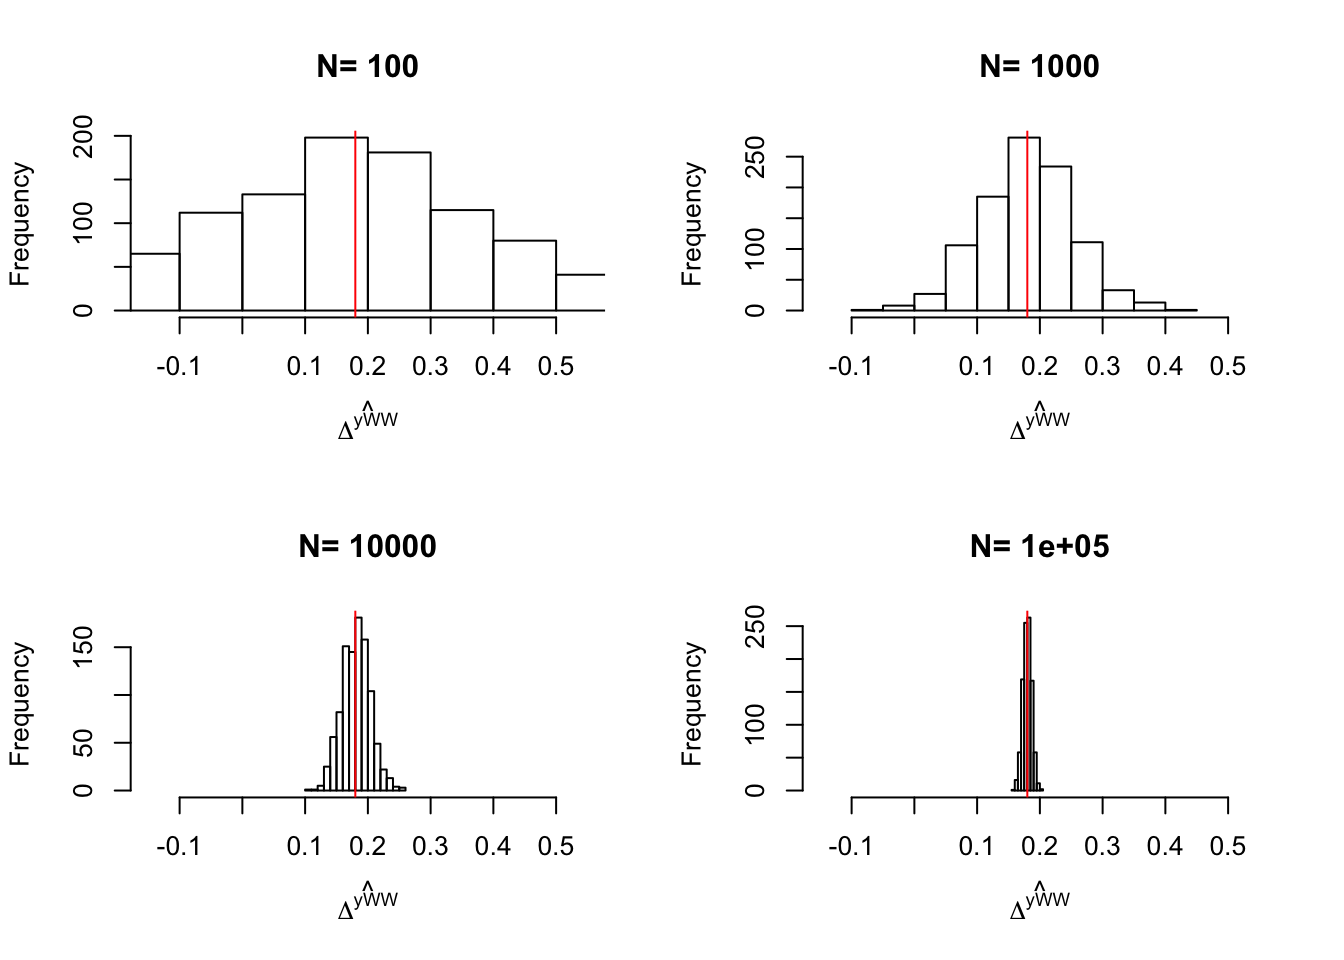
\includegraphics[width=0.6\linewidth]{STCI_files/figure-latex/montecarlo-1} 

}

\caption{Distribution of the $WW$ estimator over replications of samples of different sizes}\label{fig:montecarlo}
\end{figure}

Figure \ref{fig:montecarlo} is essential to understanding statistical
inference and the properties of our estimators. We can see on Figure
\ref{fig:montecarlo} that the estimates indeed move around at each
sample replication. We can also see that the estimates seem to be
concentrated around the truth. We also see that the estimates are more
and more concentrated around the truth as sample size grows larger and
larger.

How big is sampling noise in all of these examples? We can compute it by
using the replications as approximations to the true distribution of the
estimator after an infinite number of samples has been drawn. Let's
first choose a confidence level and then compute the empirical
equivalent to the formula in Definition \ref{def:sampnoise}.

\begin{Shaded}
\begin{Highlighting}[]
\NormalTok{delta<-}\StringTok{ }\FloatTok{0.99}
\NormalTok{delta.}\DecValTok{2}\NormalTok{ <-}\StringTok{ }\FloatTok{0.95}
\NormalTok{samp.noise <-}\StringTok{ }\ControlFlowTok{function}\NormalTok{(estim,delta)\{}
  \KeywordTok{return}\NormalTok{(}\DecValTok{2}\OperatorTok{*}\KeywordTok{quantile}\NormalTok{(}\KeywordTok{abs}\NormalTok{(}\KeywordTok{delta.y.ate}\NormalTok{(param)}\OperatorTok{-}\NormalTok{estim),}\DataTypeTok{prob=}\NormalTok{delta))}
\NormalTok{\}}
\NormalTok{samp.noise.ww <-}\StringTok{ }\KeywordTok{sapply}\NormalTok{(}\KeywordTok{lapply}\NormalTok{(simuls.ww,}\StringTok{`}\DataTypeTok{[}\StringTok{`}\NormalTok{,,}\DecValTok{1}\NormalTok{),samp.noise,}\DataTypeTok{delta=}\NormalTok{delta)}
\KeywordTok{names}\NormalTok{(samp.noise.ww) <-}\StringTok{ }\NormalTok{N.sample}
\NormalTok{samp.noise.ww}
\end{Highlighting}
\end{Shaded}

\begin{verbatim}
##        100       1000      10000      1e+05 
## 1.09916429 0.39083801 0.11582492 0.03527744
\end{verbatim}

Let's also compute precision and the signal to noise ratio and put all
of these results together in a nice table.

\begin{Shaded}
\begin{Highlighting}[]
\NormalTok{precision <-}\StringTok{ }\ControlFlowTok{function}\NormalTok{(estim,delta)\{}
  \KeywordTok{return}\NormalTok{(}\DecValTok{1}\OperatorTok{/}\KeywordTok{samp.noise}\NormalTok{(estim,delta))}
\NormalTok{\}}
\NormalTok{signal.to.noise <-}\StringTok{ }\ControlFlowTok{function}\NormalTok{(estim,delta,param)\{}
  \KeywordTok{return}\NormalTok{(}\KeywordTok{delta.y.ate}\NormalTok{(param)}\OperatorTok{/}\KeywordTok{samp.noise}\NormalTok{(estim,delta))}
\NormalTok{\}}
\NormalTok{precision.ww <-}\StringTok{ }\KeywordTok{sapply}\NormalTok{(}\KeywordTok{lapply}\NormalTok{(simuls.ww,}\StringTok{`}\DataTypeTok{[}\StringTok{`}\NormalTok{,,}\DecValTok{1}\NormalTok{),precision,}\DataTypeTok{delta=}\NormalTok{delta)}
\KeywordTok{names}\NormalTok{(precision.ww) <-}\StringTok{ }\NormalTok{N.sample}
\NormalTok{signal.to.noise.ww <-}\StringTok{ }\KeywordTok{sapply}\NormalTok{(}\KeywordTok{lapply}\NormalTok{(simuls.ww,}\StringTok{`}\DataTypeTok{[}\StringTok{`}\NormalTok{,,}\DecValTok{1}\NormalTok{),signal.to.noise,}\DataTypeTok{delta=}\NormalTok{delta,}\DataTypeTok{param=}\NormalTok{param)}
\KeywordTok{names}\NormalTok{(signal.to.noise.ww) <-}\StringTok{ }\NormalTok{N.sample}
\NormalTok{table.noise <-}\StringTok{ }\KeywordTok{cbind}\NormalTok{(samp.noise.ww,precision.ww,signal.to.noise.ww)}
\KeywordTok{colnames}\NormalTok{(table.noise) <-}\StringTok{ }\KeywordTok{c}\NormalTok{(}\StringTok{'Sampling noise'}\NormalTok{, }\StringTok{'Precision'}\NormalTok{, }\StringTok{'Signal to noise ratio'}\NormalTok{)}
\NormalTok{knitr}\OperatorTok{::}\KeywordTok{kable}\NormalTok{(table.noise,}\DataTypeTok{caption=}\KeywordTok{paste}\NormalTok{(}\StringTok{'Sampling noise of $}\CharTok{\textbackslash{}\textbackslash{}}\StringTok{hat\{WW\}$ for the population treatment effect with $}\CharTok{\textbackslash{}\textbackslash{}}\StringTok{delta=$'}\NormalTok{,delta,}\StringTok{'for various sample sizes'}\NormalTok{,}\DataTypeTok{sep=}\StringTok{' '}\NormalTok{),}\DataTypeTok{booktabs=}\OtherTok{TRUE}\NormalTok{,}\DataTypeTok{digits =} \KeywordTok{c}\NormalTok{(}\DecValTok{2}\NormalTok{,}\DecValTok{2}\NormalTok{,}\DecValTok{2}\NormalTok{),}\DataTypeTok{align=}\KeywordTok{c}\NormalTok{(}\StringTok{'c'}\NormalTok{,}\StringTok{'c'}\NormalTok{,}\StringTok{'c'}\NormalTok{))}
\end{Highlighting}
\end{Shaded}

\begin{table}[t]

\caption{\label{tab:precisionsignal}Sampling noise of $\hat{WW}$ for the population treatment effect with $\delta=$ 0.99 for various sample sizes}
\centering
\begin{tabular}{lccc}
\toprule
  & Sampling noise & Precision & Signal to noise ratio\\
\midrule
100 & 1.10 & 0.91 & 0.16\\
1000 & 0.39 & 2.56 & 0.46\\
10000 & 0.12 & 8.63 & 1.55\\
1e+05 & 0.04 & 28.35 & 5.10\\
\bottomrule
\end{tabular}
\end{table}

Finally, a nice way to summarize the extent of sampling noise is to
graph how sampling noise varies around the true treatment effect, as
shown on Figure \ref{fig:precision}.

\begin{Shaded}
\begin{Highlighting}[]
\KeywordTok{colnames}\NormalTok{(table.noise) <-}\StringTok{ }\KeywordTok{c}\NormalTok{(}\StringTok{'sampling.noise'}\NormalTok{, }\StringTok{'precision'}\NormalTok{, }\StringTok{'signal.to.noise'}\NormalTok{)}
\NormalTok{table.noise <-}\StringTok{ }\KeywordTok{as.data.frame}\NormalTok{(table.noise)}
\NormalTok{table.noise}\OperatorTok{$}\NormalTok{N <-}\StringTok{ }\KeywordTok{as.numeric}\NormalTok{(}\KeywordTok{rownames}\NormalTok{(table.noise))}
\NormalTok{table.noise}\OperatorTok{$}\NormalTok{TT <-}\StringTok{ }\KeywordTok{rep}\NormalTok{(}\KeywordTok{delta.y.ate}\NormalTok{(param),}\KeywordTok{nrow}\NormalTok{(table.noise))}
\KeywordTok{ggplot}\NormalTok{(table.noise, }\KeywordTok{aes}\NormalTok{(}\DataTypeTok{x=}\KeywordTok{as.factor}\NormalTok{(N), }\DataTypeTok{y=}\NormalTok{TT)) }\OperatorTok{+}
\StringTok{  }\KeywordTok{geom_bar}\NormalTok{(}\DataTypeTok{position=}\KeywordTok{position_dodge}\NormalTok{(), }\DataTypeTok{stat=}\StringTok{"identity"}\NormalTok{, }\DataTypeTok{colour=}\StringTok{'black'}\NormalTok{) }\OperatorTok{+}
\StringTok{  }\KeywordTok{geom_errorbar}\NormalTok{(}\KeywordTok{aes}\NormalTok{(}\DataTypeTok{ymin=}\NormalTok{TT}\OperatorTok{-}\NormalTok{sampling.noise}\OperatorTok{/}\DecValTok{2}\NormalTok{, }\DataTypeTok{ymax=}\NormalTok{TT}\OperatorTok{+}\NormalTok{sampling.noise}\OperatorTok{/}\DecValTok{2}\NormalTok{), }\DataTypeTok{width=}\NormalTok{.}\DecValTok{2}\NormalTok{,}\DataTypeTok{position=}\KeywordTok{position_dodge}\NormalTok{(.}\DecValTok{9}\NormalTok{),}\DataTypeTok{color=}\StringTok{'red'}\NormalTok{) }\OperatorTok{+}
\StringTok{  }\KeywordTok{xlab}\NormalTok{(}\StringTok{"Sample Size"}\NormalTok{)}\OperatorTok{+}
\StringTok{  }\KeywordTok{theme_bw}\NormalTok{()}
\end{Highlighting}
\end{Shaded}

\begin{figure}[htbp]

{\centering 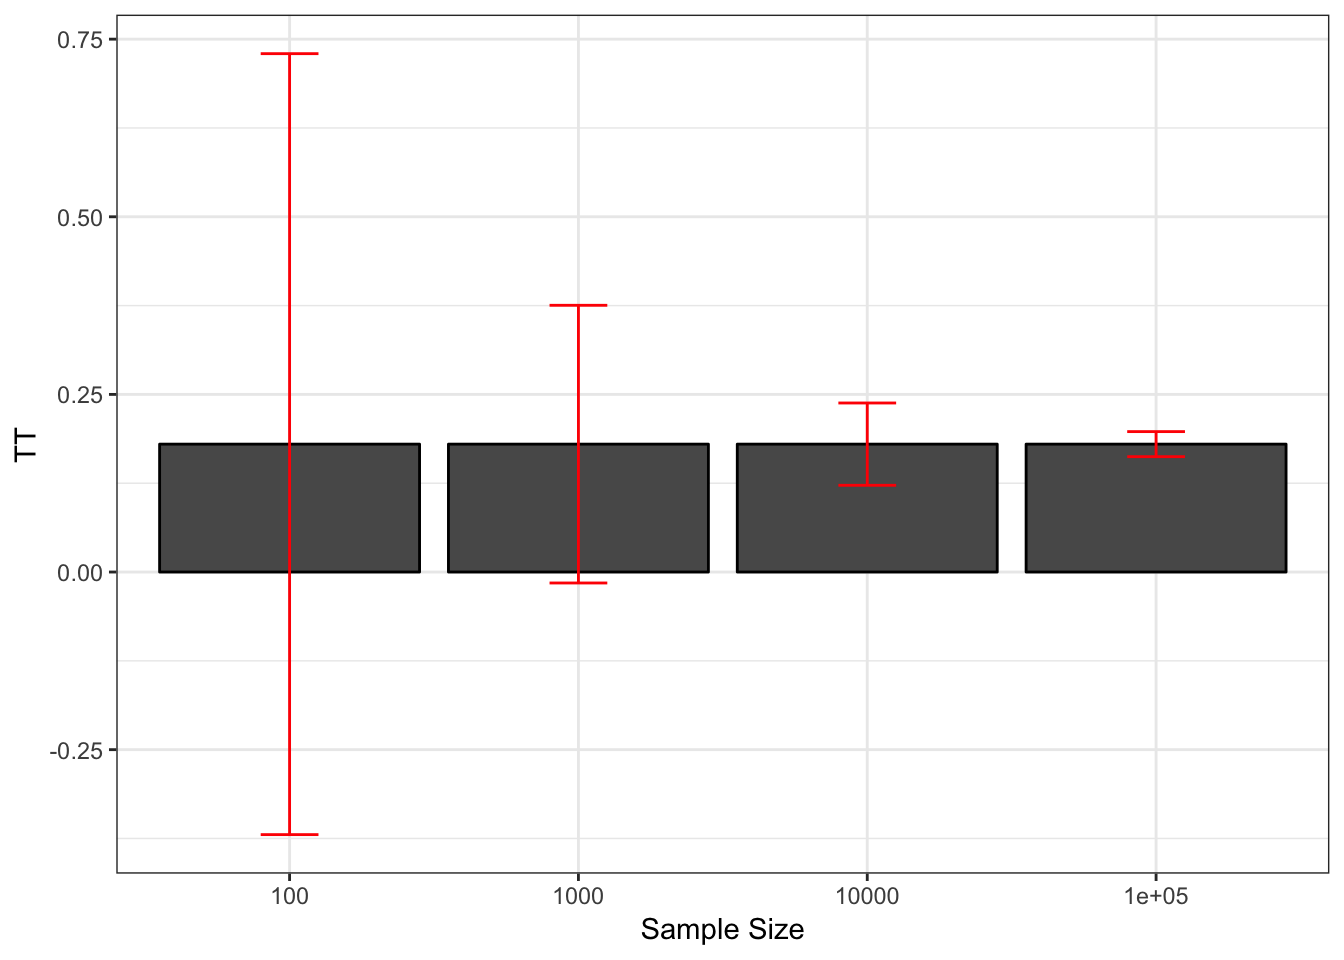
\includegraphics[width=0.6\linewidth]{STCI_files/figure-latex/precision-1} 

}

\caption{Sampling noise of $\hat{WW}$ (99\% confidence) around $TT$ for various sample sizes}\label{fig:precision}
\end{figure}

With \(N=\) 100, we can definitely see on Figure \ref{fig:precision}
that sampling noise is ridiculously large, especially compared with the
treatment effect that we are trying to estimate. The signal to noise
ratio is 0.16, which means that sampling noise is an order of magnitude
bigger than the signal we are trying to extract. As a consequence, in
22.2\% of our samples, we are going to estimate a negative effect of the
treatment. There is also a 20.4\% chance that we end up estimating an
effect that is double the true effect. So how much can we trust our
estimate from one sample to be close to the true effect of the treatment
when \(N=\) 100? Not much.

With \(N=\) 1000, sampling noise is still large: the signal to noise
ratio is 0.46, which means that sampling noise is double the signal we
are trying to extract. As a consequence, the chance that we end up with
a negative treatment effect has decreased to 0.9\% and that we end up
with an effect double the true one is 1\%. But still, the chances that
we end up with an effect that is smaller than three quarters of the true
effect is 25.6\% and the chances that we end up with an estimator that
is 25\% bigger than the true effect is 26.2\%. These are nontrivial
differences: compare a program that increases earnings by 13.5\% to one
that increases them by 18\% and another by 22.5\%. They would have
completely different cost/benefit ratios. But we at least trust our
estimator to give us a correct idea of the sign of the treatment effect
and a vague and imprecise idea of its magnitude.

With \(N=\) 10\^{}\{4\}, sampling noise is smaller than the signal,
which is encouraging. The signal to noise ratio is 1.55. In only 1\% of
the samples does the estimated effect of the treatment become smaller
than 0.125 or bigger than 0.247. We start gaining a lot of confidence in
the relative magnitude of the effect, even if sampling noise is still
responsible for economically significant variation.

With \(N=\) 10\^{}\{5\}, sampling noise has become trivial. The signal
to noise ratio is 5.1, which means that the signal is now 5 times bigger
than the sampling noise. In only 1\% of the samples does the estimated
effect of the treatment become smaller than 0.163 or bigger than 0.198.
Sampling noise is not any more responsible for economically meaningful
variation.

\subsection{Sampling noise for the sample treatment
effect}\label{sec:illusnoisesamp}

Sampling noise for the sample parameter stems from the fact that the
treated and control groups are not perfectly identical. The distribution
of observed and unobserved covariates is actually different, because of
sampling variation. This makes the actual comparison of means in the
sample a noisy estimate of the true comparison that we would obtain by
comparing the potential outcomes of the treated directly.

In order to understand this issue well and to be able to illustrate it
correctly, I am going to focus on the average treatment effect in the
whole sample, not on the treated:
\(\Delta^Y_{ATE_s}=\frac{1}{N}\sum_{i=1}^N(Y_i^1-Y_i^0)\). This enables
me to define a sample parameter that is independent of the allocation of
\(D_i\). This is without important consequences since these two
parameters are equal in the population when there is no selection bias,
as we are assuming since the beginning of this lecture. Furthermore, if
we view the treatment allocation generating no selection bias as a true
random assignment in a Randomized Controlled Trial (RCT), then it is
still possible to use this approach to estimate \(TT\) if we view the
population over which we randomise as the population selected for
receiving the treatment, as we will see in the lecture on RCTs.

\BeginKnitrBlock{example}
\protect\hypertarget{exm:unnamed-chunk-34}{}{\label{exm:unnamed-chunk-34}
}In order to assess the scope of sampling noise for our sample treatment
effect estimate, we first have to draw a sample:
\EndKnitrBlock{example}

\begin{Shaded}
\begin{Highlighting}[]
\KeywordTok{set.seed}\NormalTok{(}\DecValTok{1234}\NormalTok{)}
\NormalTok{N <-}\DecValTok{1000}
\NormalTok{mu <-}\StringTok{ }\KeywordTok{rnorm}\NormalTok{(N,param[}\StringTok{"barmu"}\NormalTok{],}\KeywordTok{sqrt}\NormalTok{(param[}\StringTok{"sigma2mu"}\NormalTok{]))}
\NormalTok{UB <-}\StringTok{ }\KeywordTok{rnorm}\NormalTok{(N,}\DecValTok{0}\NormalTok{,}\KeywordTok{sqrt}\NormalTok{(param[}\StringTok{"sigma2U"}\NormalTok{]))}
\NormalTok{yB <-}\StringTok{ }\NormalTok{mu }\OperatorTok{+}\StringTok{ }\NormalTok{UB }
\NormalTok{YB <-}\StringTok{ }\KeywordTok{exp}\NormalTok{(yB)}
\NormalTok{Ds <-}\StringTok{ }\KeywordTok{rep}\NormalTok{(}\DecValTok{0}\NormalTok{,N)}
\NormalTok{V <-}\StringTok{ }\KeywordTok{rnorm}\NormalTok{(N,param[}\StringTok{"barmu"}\NormalTok{],}\KeywordTok{sqrt}\NormalTok{(param[}\StringTok{"sigma2mu"}\NormalTok{]}\OperatorTok{+}\NormalTok{param[}\StringTok{"sigma2U"}\NormalTok{]))}
\NormalTok{Ds[V}\OperatorTok{<=}\KeywordTok{log}\NormalTok{(param[}\StringTok{"barY"}\NormalTok{])] <-}\StringTok{ }\DecValTok{1} 
\NormalTok{epsilon <-}\StringTok{ }\KeywordTok{rnorm}\NormalTok{(N,}\DecValTok{0}\NormalTok{,}\KeywordTok{sqrt}\NormalTok{(param[}\StringTok{"sigma2epsilon"}\NormalTok{]))}
\NormalTok{eta<-}\StringTok{ }\KeywordTok{rnorm}\NormalTok{(N,}\DecValTok{0}\NormalTok{,}\KeywordTok{sqrt}\NormalTok{(param[}\StringTok{"sigma2eta"}\NormalTok{]))}
\NormalTok{U0 <-}\StringTok{ }\NormalTok{param[}\StringTok{"rho"}\NormalTok{]}\OperatorTok{*}\NormalTok{UB }\OperatorTok{+}\StringTok{ }\NormalTok{epsilon}
\NormalTok{y0 <-}\StringTok{ }\NormalTok{mu }\OperatorTok{+}\StringTok{  }\NormalTok{U0 }\OperatorTok{+}\StringTok{ }\NormalTok{param[}\StringTok{"delta"}\NormalTok{]}
\NormalTok{alpha <-}\StringTok{ }\NormalTok{param[}\StringTok{"baralpha"}\NormalTok{]}\OperatorTok{+}\StringTok{  }\NormalTok{param[}\StringTok{"theta"}\NormalTok{]}\OperatorTok{*}\NormalTok{mu }\OperatorTok{+}\StringTok{ }\NormalTok{eta}
\NormalTok{y1 <-}\StringTok{ }\NormalTok{y0}\OperatorTok{+}\NormalTok{alpha}
\NormalTok{Y0 <-}\StringTok{ }\KeywordTok{exp}\NormalTok{(y0)}
\NormalTok{Y1 <-}\StringTok{ }\KeywordTok{exp}\NormalTok{(y1)}
\NormalTok{y <-}\StringTok{ }\NormalTok{y1}\OperatorTok{*}\NormalTok{Ds}\OperatorTok{+}\NormalTok{y0}\OperatorTok{*}\NormalTok{(}\DecValTok{1}\OperatorTok{-}\NormalTok{Ds)}
\NormalTok{Y <-}\StringTok{ }\NormalTok{Y1}\OperatorTok{*}\NormalTok{Ds}\OperatorTok{+}\NormalTok{Y0}\OperatorTok{*}\NormalTok{(}\DecValTok{1}\OperatorTok{-}\NormalTok{Ds)}
\end{Highlighting}
\end{Shaded}

In this sample, the treatment effect parameter is \(\Delta^y_{ATE_s}=\)
0.171. The \(WW\) estimator yields an estimate of
\(\hat{\Delta^y_{WW}}=\) 0.133. Despite random assignment, we have
\(\Delta^y_{ATE_s}\neq\hat{\Delta^y_{WW}}\), an instance of the FPSI.

In order to see how sampling noise varies, let's draw a new treatment
allocation, while retaining the same sample and the same potential
outcomes.

\begin{Shaded}
\begin{Highlighting}[]
\KeywordTok{set.seed}\NormalTok{(}\DecValTok{12345}\NormalTok{)}
\NormalTok{N <-}\DecValTok{1000}
\NormalTok{Ds <-}\StringTok{ }\KeywordTok{rep}\NormalTok{(}\DecValTok{0}\NormalTok{,N)}
\NormalTok{V <-}\StringTok{ }\KeywordTok{rnorm}\NormalTok{(N,param[}\StringTok{"barmu"}\NormalTok{],}\KeywordTok{sqrt}\NormalTok{(param[}\StringTok{"sigma2mu"}\NormalTok{]}\OperatorTok{+}\NormalTok{param[}\StringTok{"sigma2U"}\NormalTok{]))}
\NormalTok{Ds[V}\OperatorTok{<=}\KeywordTok{log}\NormalTok{(param[}\StringTok{"barY"}\NormalTok{])] <-}\StringTok{ }\DecValTok{1} 
\NormalTok{y <-}\StringTok{ }\NormalTok{y1}\OperatorTok{*}\NormalTok{Ds}\OperatorTok{+}\NormalTok{y0}\OperatorTok{*}\NormalTok{(}\DecValTok{1}\OperatorTok{-}\NormalTok{Ds)}
\NormalTok{Y <-}\StringTok{ }\NormalTok{Y1}\OperatorTok{*}\NormalTok{Ds}\OperatorTok{+}\NormalTok{Y0}\OperatorTok{*}\NormalTok{(}\DecValTok{1}\OperatorTok{-}\NormalTok{Ds)}
\end{Highlighting}
\end{Shaded}

In this sample, the treatment effect parameter is still
\(\Delta^y_{ATE_s}=\) 0.171. The \(WW\) estimator yields now an estimate
of \(\hat{\Delta^y_{WW}}=\) 0.051. The \(WW\) estimate is different from
our previous estimate because the treatment was allocated to a different
random subset of people.

Why is this second estimate so imprecise? It might because it estimates
one of the two components of the average treatment effect badly, or
both. The true average potential outcome with the treatment is, in this
sample, \(\frac{1}{N}\sum_{i=1}^Ny_i^1=\) 8.207 while the \(WW\)
estimate of this quantity is
\(\frac{1}{\sum_{i=1}^ND_i}\sum_{i=1}^ND_iy_i=\) 8.113. The true average
potential outcome without the treatment is, in this sample,
\(\frac{1}{N}\sum_{i=1}^Ny_i^0=\) 8.036 while the \(WW\) estimate of
this quantity is
\(\frac{1}{\sum_{i=1}^N(1-D_i)}\sum_{i=1}^N(1-D_i)y_i=\) 8.062. It thus
seems that most of the bias in the estimated effect stems from the fact
that the treatment has been allocated to individuals with lower than
expected outcomes with the treatment, be it because they did not react
strongly to the treatment, or because they were in worse shape without
the treatment. We can check which one of these two explanations is more
important. The true average effect of the treatment is, in this sample,
\(\frac{1}{N}\sum_{i=1}^N(y_i^1-y^0_i)=\) 0.171 while, in the treated
group, this quantity is
\(\frac{1}{\sum_{i=1}^ND_i}\sum_{i=1}^ND_i(y_i^1-y_i^0)=\) 0.18. The
true average potential outcome without the treatment is, in this sample,
\(\frac{1}{N}\sum_{i=1}^Ny^0_i=\) 8.036 while, in the treated group,
this quantity is \(\frac{1}{\sum_{i=1}^ND_i}\sum_{i=1}^ND_iy_i^0=\)
7.933. The reason for the poor performance of the \(WW\) estimator in
this sample is that individuals with lower counterfactual outcomes were
included in the treated group, not that the treatment had lower effects
on them. The bad counterfactual outcomes of the treated generates a bias
of -0.103, while the bias due to heterogeneous reactions to the
treatment is of 0.009. The last part of the bias is the one due to the
fact that the individuals in the control group have slightly better
counterfactual outcomes than in the sample: -0.026. The sum of these
three terms yields the total bias of our \(WW\) estimator in this second
sample: -0.12.

Let's now assess the overall effect of sampling noise on the estimate of
the sample treatment effect for various sample sizes. In order to do
this, I am going to use parallelized Monte Carlo simulations again. For
the sake of simplicity, I am going to generate the same potential
outcomes in each replication, using the same seed, and only choose a
different treatment allocation.

\begin{Shaded}
\begin{Highlighting}[]
\NormalTok{monte.carlo.ww.sample <-}\StringTok{ }\ControlFlowTok{function}\NormalTok{(s,N,param)\{}
  \KeywordTok{set.seed}\NormalTok{(}\DecValTok{1234}\NormalTok{)}
\NormalTok{  mu <-}\StringTok{ }\KeywordTok{rnorm}\NormalTok{(N,param[}\StringTok{"barmu"}\NormalTok{],}\KeywordTok{sqrt}\NormalTok{(param[}\StringTok{"sigma2mu"}\NormalTok{]))}
\NormalTok{  UB <-}\StringTok{ }\KeywordTok{rnorm}\NormalTok{(N,}\DecValTok{0}\NormalTok{,}\KeywordTok{sqrt}\NormalTok{(param[}\StringTok{"sigma2U"}\NormalTok{]))}
\NormalTok{  yB <-}\StringTok{ }\NormalTok{mu }\OperatorTok{+}\StringTok{ }\NormalTok{UB }
\NormalTok{  YB <-}\StringTok{ }\KeywordTok{exp}\NormalTok{(yB)}
\NormalTok{  epsilon <-}\StringTok{ }\KeywordTok{rnorm}\NormalTok{(N,}\DecValTok{0}\NormalTok{,}\KeywordTok{sqrt}\NormalTok{(param[}\StringTok{"sigma2epsilon"}\NormalTok{]))}
\NormalTok{  eta<-}\StringTok{ }\KeywordTok{rnorm}\NormalTok{(N,}\DecValTok{0}\NormalTok{,}\KeywordTok{sqrt}\NormalTok{(param[}\StringTok{"sigma2eta"}\NormalTok{]))}
\NormalTok{  U0 <-}\StringTok{ }\NormalTok{param[}\StringTok{"rho"}\NormalTok{]}\OperatorTok{*}\NormalTok{UB }\OperatorTok{+}\StringTok{ }\NormalTok{epsilon}
\NormalTok{  y0 <-}\StringTok{ }\NormalTok{mu }\OperatorTok{+}\StringTok{  }\NormalTok{U0 }\OperatorTok{+}\StringTok{ }\NormalTok{param[}\StringTok{"delta"}\NormalTok{]}
\NormalTok{  alpha <-}\StringTok{ }\NormalTok{param[}\StringTok{"baralpha"}\NormalTok{]}\OperatorTok{+}\StringTok{  }\NormalTok{param[}\StringTok{"theta"}\NormalTok{]}\OperatorTok{*}\NormalTok{mu }\OperatorTok{+}\StringTok{ }\NormalTok{eta}
\NormalTok{  y1 <-}\StringTok{ }\NormalTok{y0}\OperatorTok{+}\NormalTok{alpha}
\NormalTok{  Y0 <-}\StringTok{ }\KeywordTok{exp}\NormalTok{(y0)}
\NormalTok{  Y1 <-}\StringTok{ }\KeywordTok{exp}\NormalTok{(y1)}
  \KeywordTok{set.seed}\NormalTok{(s)}
\NormalTok{  Ds <-}\StringTok{ }\KeywordTok{rep}\NormalTok{(}\DecValTok{0}\NormalTok{,N)}
\NormalTok{  V <-}\StringTok{ }\KeywordTok{rnorm}\NormalTok{(N,param[}\StringTok{"barmu"}\NormalTok{],}\KeywordTok{sqrt}\NormalTok{(param[}\StringTok{"sigma2mu"}\NormalTok{]}\OperatorTok{+}\NormalTok{param[}\StringTok{"sigma2U"}\NormalTok{]))}
\NormalTok{  Ds[V}\OperatorTok{<=}\KeywordTok{log}\NormalTok{(param[}\StringTok{"barY"}\NormalTok{])] <-}\StringTok{ }\DecValTok{1} 
\NormalTok{  y <-}\StringTok{ }\NormalTok{y1}\OperatorTok{*}\NormalTok{Ds}\OperatorTok{+}\NormalTok{y0}\OperatorTok{*}\NormalTok{(}\DecValTok{1}\OperatorTok{-}\NormalTok{Ds)}
\NormalTok{  Y <-}\StringTok{ }\NormalTok{Y1}\OperatorTok{*}\NormalTok{Ds}\OperatorTok{+}\NormalTok{Y0}\OperatorTok{*}\NormalTok{(}\DecValTok{1}\OperatorTok{-}\NormalTok{Ds)}
  \KeywordTok{return}\NormalTok{((}\DecValTok{1}\OperatorTok{/}\KeywordTok{sum}\NormalTok{(Ds))}\OperatorTok{*}\KeywordTok{sum}\NormalTok{(y}\OperatorTok{*}\NormalTok{Ds)}\OperatorTok{-}\NormalTok{(}\DecValTok{1}\OperatorTok{/}\KeywordTok{sum}\NormalTok{(}\DecValTok{1}\OperatorTok{-}\NormalTok{Ds))}\OperatorTok{*}\KeywordTok{sum}\NormalTok{(y}\OperatorTok{*}\NormalTok{(}\DecValTok{1}\OperatorTok{-}\NormalTok{Ds)))}
\NormalTok{\}}

\NormalTok{simuls.ww.N.sample <-}\StringTok{ }\ControlFlowTok{function}\NormalTok{(N,Nsim,param)\{}
  \KeywordTok{return}\NormalTok{(}\KeywordTok{unlist}\NormalTok{(}\KeywordTok{lapply}\NormalTok{(}\DecValTok{1}\OperatorTok{:}\NormalTok{Nsim,monte.carlo.ww.sample,}\DataTypeTok{N=}\NormalTok{N,}\DataTypeTok{param=}\NormalTok{param)))}
\NormalTok{\}}

\NormalTok{sf.simuls.ww.N.sample <-}\StringTok{ }\ControlFlowTok{function}\NormalTok{(N,Nsim,param)\{}
  \KeywordTok{sfInit}\NormalTok{(}\DataTypeTok{parallel=}\OtherTok{TRUE}\NormalTok{,}\DataTypeTok{cpus=}\NormalTok{ncpus)}
\NormalTok{  sim <-}\StringTok{ }\KeywordTok{sfLapply}\NormalTok{(}\DecValTok{1}\OperatorTok{:}\NormalTok{Nsim,monte.carlo.ww.sample,}\DataTypeTok{N=}\NormalTok{N,}\DataTypeTok{param=}\NormalTok{param)}
  \KeywordTok{sfStop}\NormalTok{()}
  \KeywordTok{return}\NormalTok{(}\KeywordTok{unlist}\NormalTok{(sim))}
\NormalTok{\}}

\NormalTok{simuls.ww.sample <-}\StringTok{ }\KeywordTok{lapply}\NormalTok{(N.sample,sf.simuls.ww.N.sample,}\DataTypeTok{Nsim=}\NormalTok{Nsim,}\DataTypeTok{param=}\NormalTok{param)}

\NormalTok{monte.carlo.ate.sample <-}\StringTok{ }\ControlFlowTok{function}\NormalTok{(N,s,param)\{}
  \KeywordTok{set.seed}\NormalTok{(s)}
\NormalTok{  mu <-}\StringTok{ }\KeywordTok{rnorm}\NormalTok{(N,param[}\StringTok{"barmu"}\NormalTok{],}\KeywordTok{sqrt}\NormalTok{(param[}\StringTok{"sigma2mu"}\NormalTok{]))}
\NormalTok{  UB <-}\StringTok{ }\KeywordTok{rnorm}\NormalTok{(N,}\DecValTok{0}\NormalTok{,}\KeywordTok{sqrt}\NormalTok{(param[}\StringTok{"sigma2U"}\NormalTok{]))}
\NormalTok{  yB <-}\StringTok{ }\NormalTok{mu }\OperatorTok{+}\StringTok{ }\NormalTok{UB }
\NormalTok{  YB <-}\StringTok{ }\KeywordTok{exp}\NormalTok{(yB)}
\NormalTok{  epsilon <-}\StringTok{ }\KeywordTok{rnorm}\NormalTok{(N,}\DecValTok{0}\NormalTok{,}\KeywordTok{sqrt}\NormalTok{(param[}\StringTok{"sigma2epsilon"}\NormalTok{]))}
\NormalTok{  eta<-}\StringTok{ }\KeywordTok{rnorm}\NormalTok{(N,}\DecValTok{0}\NormalTok{,}\KeywordTok{sqrt}\NormalTok{(param[}\StringTok{"sigma2eta"}\NormalTok{]))}
\NormalTok{  U0 <-}\StringTok{ }\NormalTok{param[}\StringTok{"rho"}\NormalTok{]}\OperatorTok{*}\NormalTok{UB }\OperatorTok{+}\StringTok{ }\NormalTok{epsilon}
\NormalTok{  y0 <-}\StringTok{ }\NormalTok{mu }\OperatorTok{+}\StringTok{  }\NormalTok{U0 }\OperatorTok{+}\StringTok{ }\NormalTok{param[}\StringTok{"delta"}\NormalTok{]}
\NormalTok{  alpha <-}\StringTok{ }\NormalTok{param[}\StringTok{"baralpha"}\NormalTok{]}\OperatorTok{+}\StringTok{  }\NormalTok{param[}\StringTok{"theta"}\NormalTok{]}\OperatorTok{*}\NormalTok{mu }\OperatorTok{+}\StringTok{ }\NormalTok{eta}
\NormalTok{  y1 <-}\StringTok{ }\NormalTok{y0}\OperatorTok{+}\NormalTok{alpha}
\NormalTok{  Y0 <-}\StringTok{ }\KeywordTok{exp}\NormalTok{(y0)}
\NormalTok{  Y1 <-}\StringTok{ }\KeywordTok{exp}\NormalTok{(y1)}
\NormalTok{  Ds <-}\StringTok{ }\KeywordTok{rep}\NormalTok{(}\DecValTok{0}\NormalTok{,N)}
\NormalTok{  V <-}\StringTok{ }\KeywordTok{rnorm}\NormalTok{(N,param[}\StringTok{"barmu"}\NormalTok{],}\KeywordTok{sqrt}\NormalTok{(param[}\StringTok{"sigma2mu"}\NormalTok{]}\OperatorTok{+}\NormalTok{param[}\StringTok{"sigma2U"}\NormalTok{]))}
\NormalTok{  Ds[V}\OperatorTok{<=}\KeywordTok{log}\NormalTok{(param[}\StringTok{"barY"}\NormalTok{])] <-}\StringTok{ }\DecValTok{1} 
\NormalTok{  y <-}\StringTok{ }\NormalTok{y1}\OperatorTok{*}\NormalTok{Ds}\OperatorTok{+}\NormalTok{y0}\OperatorTok{*}\NormalTok{(}\DecValTok{1}\OperatorTok{-}\NormalTok{Ds)}
\NormalTok{  Y <-}\StringTok{ }\NormalTok{Y1}\OperatorTok{*}\NormalTok{Ds}\OperatorTok{+}\NormalTok{Y0}\OperatorTok{*}\NormalTok{(}\DecValTok{1}\OperatorTok{-}\NormalTok{Ds)}
  \KeywordTok{return}\NormalTok{(}\KeywordTok{mean}\NormalTok{(alpha))}
\NormalTok{\}}

\KeywordTok{par}\NormalTok{(}\DataTypeTok{mfrow=}\KeywordTok{c}\NormalTok{(}\DecValTok{2}\NormalTok{,}\DecValTok{2}\NormalTok{))}
\ControlFlowTok{for}\NormalTok{ (i }\ControlFlowTok{in} \DecValTok{1}\OperatorTok{:}\DecValTok{4}\NormalTok{)\{}
  \KeywordTok{hist}\NormalTok{(simuls.ww.sample[[i]],}\DataTypeTok{main=}\KeywordTok{paste}\NormalTok{(}\StringTok{'N='}\NormalTok{,}\KeywordTok{as.character}\NormalTok{(N.sample[i])),}\DataTypeTok{xlab=}\KeywordTok{expression}\NormalTok{(}\KeywordTok{hat}\NormalTok{(Delta}\OperatorTok{^}\NormalTok{yWW)),}\DataTypeTok{xlim=}\KeywordTok{c}\NormalTok{(}\OperatorTok{-}\FloatTok{0.15}\NormalTok{,}\FloatTok{0.55}\NormalTok{))}
  \KeywordTok{abline}\NormalTok{(}\DataTypeTok{v=}\KeywordTok{monte.carlo.ate.sample}\NormalTok{(N.sample[[i]],}\DecValTok{1234}\NormalTok{,param),}\DataTypeTok{col=}\StringTok{"red"}\NormalTok{)}
\NormalTok{\}}
\end{Highlighting}
\end{Shaded}

\begin{figure}[htbp]

{\centering 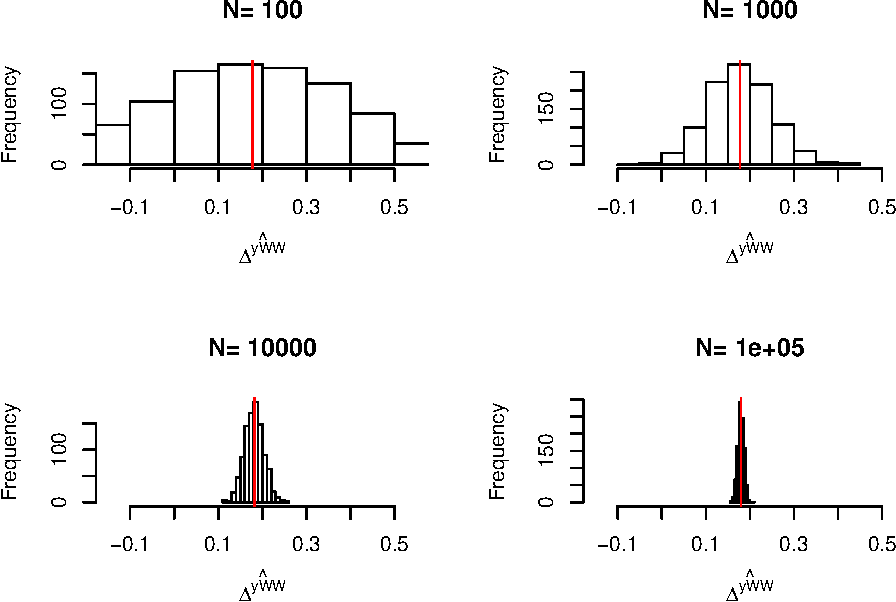
\includegraphics[width=0.6\linewidth]{STCI_files/figure-latex/montecarlosample-1} 

}

\caption{Distribution of the $WW$ estimator over replications of treatment allocation for samples of different sizes}\label{fig:montecarlosample}
\end{figure}

Let's also compute sampling noise, precision and the signal to noise
ratio in these examples.

\begin{Shaded}
\begin{Highlighting}[]
\NormalTok{samp.noise.sample <-}\StringTok{ }\ControlFlowTok{function}\NormalTok{(i,delta,param)\{}
  \KeywordTok{return}\NormalTok{(}\DecValTok{2}\OperatorTok{*}\KeywordTok{quantile}\NormalTok{(}\KeywordTok{abs}\NormalTok{(}\KeywordTok{monte.carlo.ate.sample}\NormalTok{(}\DecValTok{1234}\NormalTok{,N.sample[[i]],param)}\OperatorTok{-}\NormalTok{simuls.ww.sample[[i]]),}\DataTypeTok{prob=}\NormalTok{delta))}
\NormalTok{\}}
\NormalTok{samp.noise.ww.sample <-}\StringTok{ }\KeywordTok{sapply}\NormalTok{(}\DecValTok{1}\OperatorTok{:}\DecValTok{4}\NormalTok{,samp.noise.sample,}\DataTypeTok{delta=}\NormalTok{delta,}\DataTypeTok{param=}\NormalTok{param)}
\KeywordTok{names}\NormalTok{(samp.noise.ww.sample) <-}\StringTok{ }\NormalTok{N.sample}

\NormalTok{precision.sample <-}\StringTok{ }\ControlFlowTok{function}\NormalTok{(i,delta,param)\{}
  \KeywordTok{return}\NormalTok{(}\DecValTok{1}\OperatorTok{/}\KeywordTok{samp.noise.sample}\NormalTok{(i,delta,}\DataTypeTok{param=}\NormalTok{param))}
\NormalTok{\}}
\NormalTok{signal.to.noise.sample <-}\StringTok{ }\ControlFlowTok{function}\NormalTok{(i,delta,param)\{}
  \KeywordTok{return}\NormalTok{(}\KeywordTok{monte.carlo.ate.sample}\NormalTok{(}\DecValTok{1234}\NormalTok{,N.sample[[i]],param)}\OperatorTok{/}\KeywordTok{samp.noise.sample}\NormalTok{(i,delta,}\DataTypeTok{param=}\NormalTok{param))}
\NormalTok{\}}
\NormalTok{precision.ww.sample <-}\StringTok{ }\KeywordTok{sapply}\NormalTok{(}\DecValTok{1}\OperatorTok{:}\DecValTok{4}\NormalTok{,precision.sample,}\DataTypeTok{delta=}\NormalTok{delta,}\DataTypeTok{param=}\NormalTok{param)}
\KeywordTok{names}\NormalTok{(precision.ww.sample) <-}\StringTok{ }\NormalTok{N.sample}
\NormalTok{signal.to.noise.ww.sample <-}\StringTok{ }\KeywordTok{sapply}\NormalTok{(}\DecValTok{1}\OperatorTok{:}\DecValTok{4}\NormalTok{,signal.to.noise.sample,}\DataTypeTok{delta=}\NormalTok{delta,}\DataTypeTok{param=}\NormalTok{param)}
\KeywordTok{names}\NormalTok{(signal.to.noise.ww.sample) <-}\StringTok{ }\NormalTok{N.sample}
\NormalTok{table.noise.sample <-}\StringTok{ }\KeywordTok{cbind}\NormalTok{(samp.noise.ww.sample,precision.ww.sample,signal.to.noise.ww.sample)}
\KeywordTok{colnames}\NormalTok{(table.noise.sample) <-}\StringTok{ }\KeywordTok{c}\NormalTok{(}\StringTok{'Sampling noise'}\NormalTok{, }\StringTok{'Precision'}\NormalTok{, }\StringTok{'Signal to noise ratio'}\NormalTok{)}
\NormalTok{knitr}\OperatorTok{::}\KeywordTok{kable}\NormalTok{(table.noise.sample,}\DataTypeTok{caption=}\KeywordTok{paste}\NormalTok{(}\StringTok{'Sampling noise of $}\CharTok{\textbackslash{}\textbackslash{}}\StringTok{hat\{WW\}$ for the sample treatment effect with $}\CharTok{\textbackslash{}\textbackslash{}}\StringTok{delta=$'}\NormalTok{,delta,}\StringTok{'and for various sample sizes'}\NormalTok{,}\DataTypeTok{sep=}\StringTok{' '}\NormalTok{),}\DataTypeTok{booktabs=}\OtherTok{TRUE}\NormalTok{,}\DataTypeTok{align=}\KeywordTok{c}\NormalTok{(}\StringTok{'c'}\NormalTok{,}\StringTok{'c'}\NormalTok{,}\StringTok{'c'}\NormalTok{),}\DataTypeTok{digits=}\KeywordTok{c}\NormalTok{(}\DecValTok{3}\NormalTok{,}\DecValTok{3}\NormalTok{,}\DecValTok{3}\NormalTok{))}
\end{Highlighting}
\end{Shaded}

\begin{table}[t]

\caption{\label{tab:sampnoisesample}Sampling noise of $\hat{WW}$ for the sample treatment effect with $\delta=$ 0.99 and for various sample sizes}
\centering
\begin{tabular}{lccc}
\toprule
  & Sampling noise & Precision & Signal to noise ratio\\
\midrule
100 & 1.208 & 0.828 & 0.149\\
1000 & 0.366 & 2.729 & 0.482\\
10000 & 0.122 & 8.218 & 1.585\\
1e+05 & 0.033 & 30.283 & 5.453\\
\bottomrule
\end{tabular}
\end{table}

Finally, let's compare the extent of sampling noise for the population
and the sample treatment effect parameters.

\begin{Shaded}
\begin{Highlighting}[]
\KeywordTok{colnames}\NormalTok{(table.noise.sample) <-}\StringTok{ }\KeywordTok{c}\NormalTok{(}\StringTok{'sampling.noise'}\NormalTok{, }\StringTok{'precision'}\NormalTok{, }\StringTok{'signal.to.noise'}\NormalTok{)}
\NormalTok{table.noise.sample <-}\StringTok{ }\KeywordTok{as.data.frame}\NormalTok{(table.noise.sample)}
\NormalTok{table.noise.sample}\OperatorTok{$}\NormalTok{N <-}\StringTok{ }\KeywordTok{as.numeric}\NormalTok{(}\KeywordTok{rownames}\NormalTok{(table.noise.sample))}
\NormalTok{table.noise.sample}\OperatorTok{$}\NormalTok{TT <-}\StringTok{ }\KeywordTok{sapply}\NormalTok{(N.sample,monte.carlo.ate.sample,}\DataTypeTok{s=}\DecValTok{1234}\NormalTok{,}\DataTypeTok{param=}\NormalTok{param)}
\NormalTok{table.noise.sample}\OperatorTok{$}\NormalTok{Type <-}\StringTok{ 'TTs'}
\NormalTok{table.noise}\OperatorTok{$}\NormalTok{Type <-}\StringTok{ 'TT'}
\NormalTok{table.noise.tot <-}\StringTok{ }\KeywordTok{rbind}\NormalTok{(table.noise,table.noise.sample)}
\NormalTok{table.noise.tot}\OperatorTok{$}\NormalTok{Type <-}\StringTok{ }\KeywordTok{factor}\NormalTok{(table.noise.tot}\OperatorTok{$}\NormalTok{Type)}

\KeywordTok{ggplot}\NormalTok{(table.noise.tot, }\KeywordTok{aes}\NormalTok{(}\DataTypeTok{x=}\KeywordTok{as.factor}\NormalTok{(N), }\DataTypeTok{y=}\NormalTok{TT,}\DataTypeTok{fill=}\NormalTok{Type)) }\OperatorTok{+}
\StringTok{  }\KeywordTok{geom_bar}\NormalTok{(}\DataTypeTok{position=}\KeywordTok{position_dodge}\NormalTok{(), }\DataTypeTok{stat=}\StringTok{"identity"}\NormalTok{, }\DataTypeTok{colour=}\StringTok{'black'}\NormalTok{) }\OperatorTok{+}
\StringTok{  }\KeywordTok{geom_errorbar}\NormalTok{(}\KeywordTok{aes}\NormalTok{(}\DataTypeTok{ymin=}\NormalTok{TT}\OperatorTok{-}\NormalTok{sampling.noise}\OperatorTok{/}\DecValTok{2}\NormalTok{, }\DataTypeTok{ymax=}\NormalTok{TT}\OperatorTok{+}\NormalTok{sampling.noise}\OperatorTok{/}\DecValTok{2}\NormalTok{), }\DataTypeTok{width=}\NormalTok{.}\DecValTok{2}\NormalTok{,}\DataTypeTok{position=}\KeywordTok{position_dodge}\NormalTok{(.}\DecValTok{9}\NormalTok{),}\DataTypeTok{color=}\StringTok{'red'}\NormalTok{) }\OperatorTok{+}
\StringTok{  }\KeywordTok{xlab}\NormalTok{(}\StringTok{"Sample Size"}\NormalTok{)}\OperatorTok{+}
\StringTok{  }\KeywordTok{theme_bw}\NormalTok{()}\OperatorTok{+}
\StringTok{  }\KeywordTok{theme}\NormalTok{(}\DataTypeTok{legend.position=}\KeywordTok{c}\NormalTok{(}\FloatTok{0.85}\NormalTok{,}\FloatTok{0.88}\NormalTok{))}
\end{Highlighting}
\end{Shaded}

\begin{figure}[htbp]

{\centering 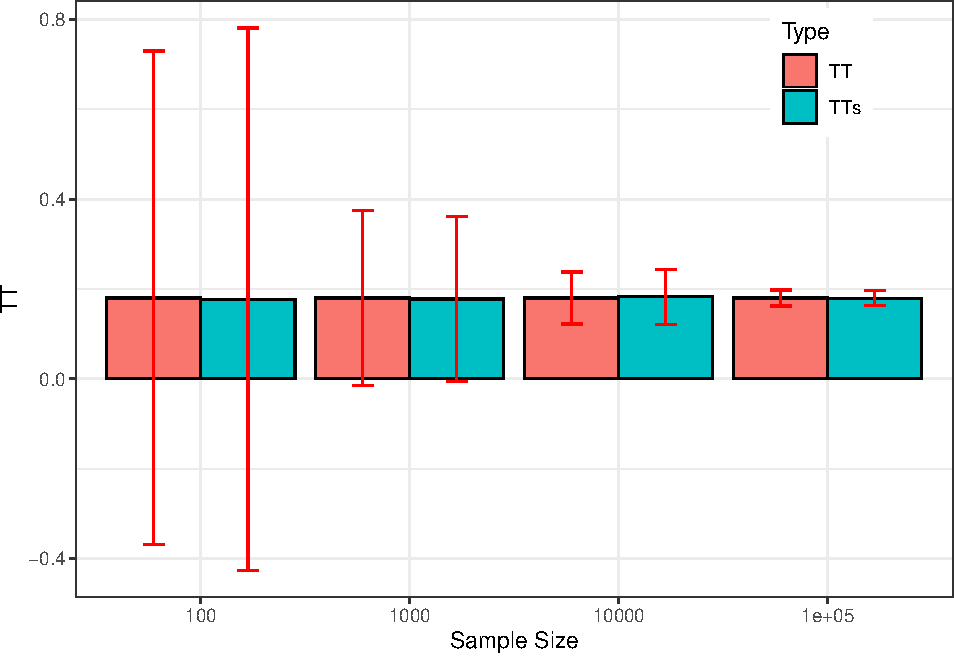
\includegraphics[width=0.6\linewidth]{STCI_files/figure-latex/precisionpopsample-1} 

}

\caption{Sampling noise of $\hat{WW}$ (99\% confidence) around $TT$ and $TT_s$ for various sample sizes}\label{fig:precisionpopsample}
\end{figure}

Figure \ref{fig:montecarlosample} and Table \ref{tab:sampnoisesample}
present the results of the simulations of sampling noise for the sample
treatment effect parameter. Figure \ref{fig:precisionpopsample} compares
sampling noise for the population and sample treatment effects.\\
For all practical purposes, the estimates of sampling noise for the
sample treatment effect are extremely close to the ones we have
estimated for the population treatment effect. I am actually surprised
by this result, since I expected that keeping the potential outcomes
constant over replications would decrease sampling noise. It seems that
the variability in potential outcomes over replications of random
allocations of the treatment in a given sample mimicks very well the
sampling process from a population. I do not know if this result of
similarity of sampling noise for the population and sample treatment
effect is a general one, but considering them as similar or close seems
innocuous in our example.

\subsection{Building confidence intervals from estimates of sampling
noise}\label{sec:confinterv}

In real life, we do not observe \(TT\). We only have access to
\(\hat{E}\). Let's also assume for now that we have access to an
estimate of sampling noise, \(2\epsilon\). How can we use these two
quantities to assess the set of values that \(TT\) might take? One very
useful device that we can use is the confidence interval. Confidence
intervals are very useful because they quantify the zone within which we
have a chance to find the true effect \(TT\):

\BeginKnitrBlock{theorem}[Confidence interval]
\protect\hypertarget{thm:confinter}{}{\label{thm:confinter}
\iffalse (Confidence interval) \fi{} }For a given level of confidence
\(\delta\) and corresponding level of sampling noise \(2\epsilon\) of
the estimator \(\hat{E}\) of \(TT\), the confidence interval
\(\left\{\hat{E}-\epsilon,\hat{E}+\epsilon\right\}\) is such that the
probability that it contains \(TT\) is equal to \(\delta\) over sample
replications:

\begin{align*}
  \Pr(\hat{E}-\epsilon\leq TT\leq\hat{E}+\epsilon) & = \delta.
\end{align*}
\EndKnitrBlock{theorem}

\BeginKnitrBlock{proof}
\iffalse{} {Proof. } \fi{}From the definition of sampling noise, we know
that:

\begin{align*}
  \Pr(|\hat{E}-TT|\leq\epsilon) & = \delta.
\end{align*}

Now:

\begin{align*}
  \Pr(|\hat{E}-TT|\leq\epsilon) & = \Pr(TT-\epsilon\leq\hat{E}\leq TT+\epsilon)\\
                                & = \Pr(-\hat{E}-\epsilon\leq-TT\leq -\hat{E}+\epsilon)\\
                                & = \Pr(\hat{E}-\epsilon\leq TT\leq\hat{E}+\epsilon),
\end{align*}

which proves the result.
\EndKnitrBlock{proof}

It is very important to note that confidence intervals are centered
around \(\hat{E}\) and not around \(TT\). When estimating sampling noise
and building Figure \ref{fig:precision}, we have centered our intervals
around \(TT\). The interval was fixed and \(\hat{E}\) was moving across
replications and \(2\epsilon\) was defined as the length of the interval
around \(TT\) containing a proportion \(\delta\) of the estimates
\(\hat{E}\). A confidence interval cannot be centered around \(TT\),
which is unknown, but is centered around \(\hat{E}\), that we can
observe. As a consequence, it is the interval that moves around across
replications, and \(\delta\) is the proportion of samples in which the
interval contains \(TT\).

\BeginKnitrBlock{example}
\protect\hypertarget{exm:unnamed-chunk-36}{}{\label{exm:unnamed-chunk-36}
}Let's see how confidence intervals behave in our numerical example.
\EndKnitrBlock{example}

\begin{Shaded}
\begin{Highlighting}[]
\NormalTok{N.plot <-}\StringTok{ }\DecValTok{40}
\NormalTok{plot.list <-}\StringTok{ }\KeywordTok{list}\NormalTok{()}

\ControlFlowTok{for}\NormalTok{ (k }\ControlFlowTok{in} \DecValTok{1}\OperatorTok{:}\KeywordTok{length}\NormalTok{(N.sample))\{}
  \KeywordTok{set.seed}\NormalTok{(}\DecValTok{1234}\NormalTok{)}
\NormalTok{  test <-}\StringTok{ }\KeywordTok{sample}\NormalTok{(simuls.ww[[k]][,}\StringTok{'WW'}\NormalTok{],N.plot)}
\NormalTok{  test <-}\StringTok{ }\KeywordTok{as.data.frame}\NormalTok{(}\KeywordTok{cbind}\NormalTok{(test,}\KeywordTok{rep}\NormalTok{(}\KeywordTok{samp.noise}\NormalTok{(simuls.ww[[k]][,}\StringTok{'WW'}\NormalTok{],}\DataTypeTok{delta=}\NormalTok{delta)),}\KeywordTok{rep}\NormalTok{(}\KeywordTok{samp.noise}\NormalTok{(simuls.ww[[k]][,}\StringTok{'WW'}\NormalTok{],}\DataTypeTok{delta=}\NormalTok{delta.}\DecValTok{2}\NormalTok{))))}
  \KeywordTok{colnames}\NormalTok{(test) <-}\StringTok{ }\KeywordTok{c}\NormalTok{(}\StringTok{'WW'}\NormalTok{,}\StringTok{'sampling.noise.1'}\NormalTok{,}\StringTok{'sampling.noise.2'}\NormalTok{)}
\NormalTok{  test}\OperatorTok{$}\NormalTok{id <-}\StringTok{ }\DecValTok{1}\OperatorTok{:}\NormalTok{N.plot}
\NormalTok{  plot.test <-}\StringTok{ }\KeywordTok{ggplot}\NormalTok{(test, }\KeywordTok{aes}\NormalTok{(}\DataTypeTok{x=}\KeywordTok{as.factor}\NormalTok{(id), }\DataTypeTok{y=}\NormalTok{WW)) }\OperatorTok{+}
\StringTok{      }\KeywordTok{geom_bar}\NormalTok{(}\DataTypeTok{position=}\KeywordTok{position_dodge}\NormalTok{(), }\DataTypeTok{stat=}\StringTok{"identity"}\NormalTok{, }\DataTypeTok{colour=}\StringTok{'black'}\NormalTok{) }\OperatorTok{+}
\StringTok{      }\KeywordTok{geom_errorbar}\NormalTok{(}\KeywordTok{aes}\NormalTok{(}\DataTypeTok{ymin=}\NormalTok{WW}\OperatorTok{-}\NormalTok{sampling.noise.}\DecValTok{1}\OperatorTok{/}\DecValTok{2}\NormalTok{, }\DataTypeTok{ymax=}\NormalTok{WW}\OperatorTok{+}\NormalTok{sampling.noise.}\DecValTok{1}\OperatorTok{/}\DecValTok{2}\NormalTok{), }\DataTypeTok{width=}\NormalTok{.}\DecValTok{2}\NormalTok{,}\DataTypeTok{position=}\KeywordTok{position_dodge}\NormalTok{(.}\DecValTok{9}\NormalTok{),}\DataTypeTok{color=}\StringTok{'red'}\NormalTok{) }\OperatorTok{+}
\StringTok{      }\KeywordTok{geom_errorbar}\NormalTok{(}\KeywordTok{aes}\NormalTok{(}\DataTypeTok{ymin=}\NormalTok{WW}\OperatorTok{-}\NormalTok{sampling.noise.}\DecValTok{2}\OperatorTok{/}\DecValTok{2}\NormalTok{, }\DataTypeTok{ymax=}\NormalTok{WW}\OperatorTok{+}\NormalTok{sampling.noise.}\DecValTok{2}\OperatorTok{/}\DecValTok{2}\NormalTok{), }\DataTypeTok{width=}\NormalTok{.}\DecValTok{2}\NormalTok{,}\DataTypeTok{position=}\KeywordTok{position_dodge}\NormalTok{(.}\DecValTok{9}\NormalTok{),}\DataTypeTok{color=}\StringTok{'blue'}\NormalTok{) }\OperatorTok{+}
\StringTok{      }\KeywordTok{geom_hline}\NormalTok{(}\KeywordTok{aes}\NormalTok{(}\DataTypeTok{yintercept=}\KeywordTok{delta.y.ate}\NormalTok{(param)), }\DataTypeTok{colour=}\StringTok{"#990000"}\NormalTok{, }\DataTypeTok{linetype=}\StringTok{"dashed"}\NormalTok{)}\OperatorTok{+}
\StringTok{      }\CommentTok{#ylim(-0.5,1.2)+}
\StringTok{      }\KeywordTok{xlab}\NormalTok{(}\StringTok{"Sample id"}\NormalTok{)}\OperatorTok{+}
\StringTok{      }\KeywordTok{theme_bw}\NormalTok{()}\OperatorTok{+}
\StringTok{      }\KeywordTok{ggtitle}\NormalTok{(}\KeywordTok{paste}\NormalTok{(}\StringTok{"N="}\NormalTok{,N.sample[k]))}
\NormalTok{  plot.list[[k]] <-}\StringTok{ }\NormalTok{plot.test }
\NormalTok{\}}
\NormalTok{plot.CI <-}\StringTok{ }\KeywordTok{plot_grid}\NormalTok{(plot.list[[}\DecValTok{1}\NormalTok{]],plot.list[[}\DecValTok{2}\NormalTok{]],plot.list[[}\DecValTok{3}\NormalTok{]],plot.list[[}\DecValTok{4}\NormalTok{]],}\DataTypeTok{ncol=}\DecValTok{1}\NormalTok{,}\DataTypeTok{nrow=}\KeywordTok{length}\NormalTok{(N.sample))}
\KeywordTok{print}\NormalTok{(plot.CI)}
\end{Highlighting}
\end{Shaded}

\begin{figure}[htbp]

{\centering 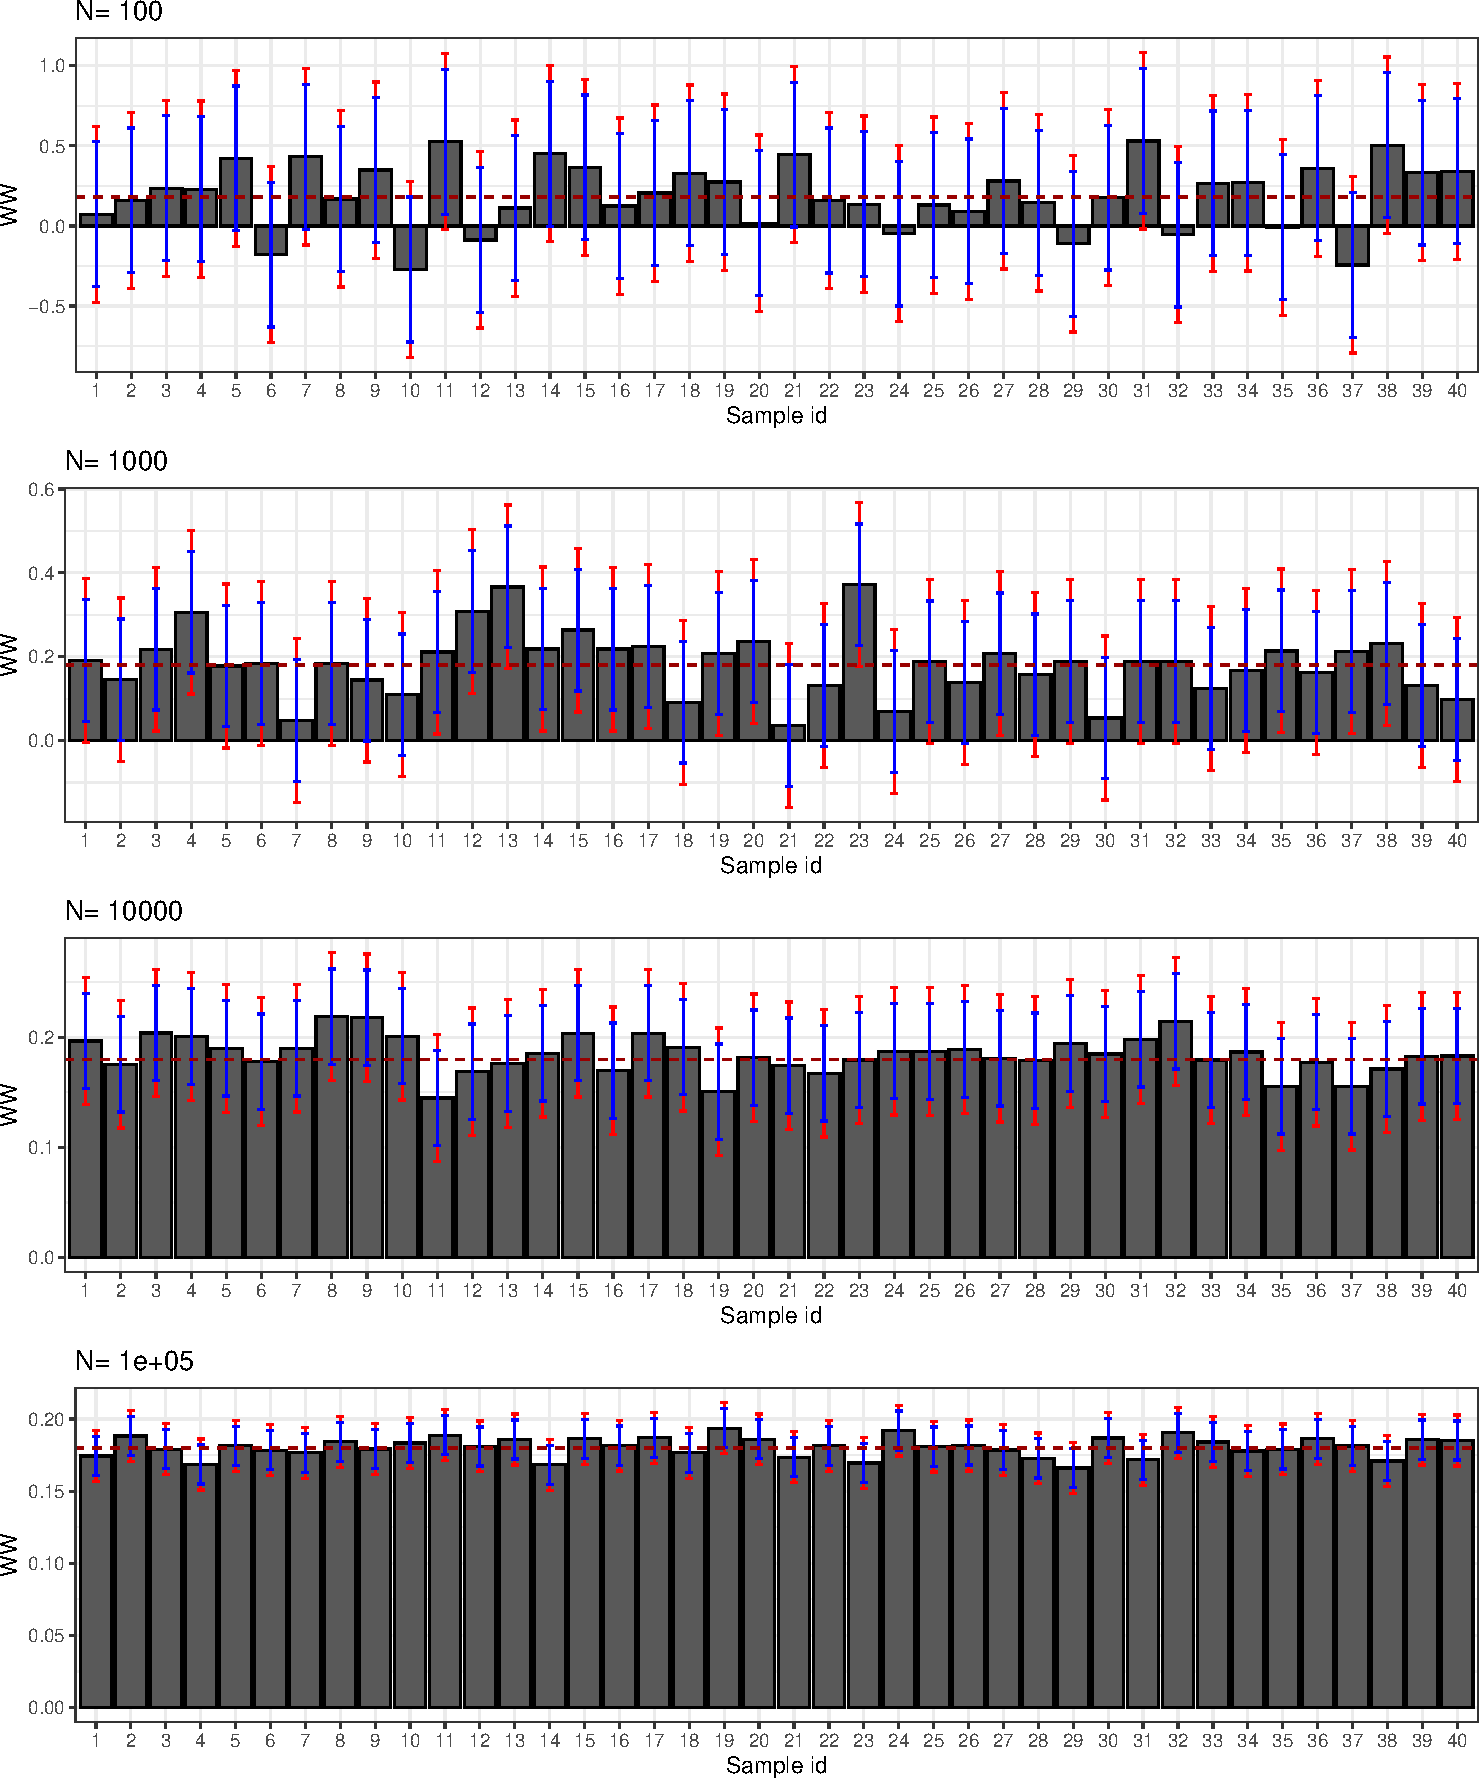
\includegraphics[width=0.6\linewidth]{STCI_files/figure-latex/confinterval-1} 

}

\caption{Confidence intervals of $\hat{WW}$ for $\delta=$ 0.99 (red) and 0.95 (blue) over sample replications for various sample sizes}\label{fig:confinterval}
\end{figure}

Figure \ref{fig:confinterval} presents the 99\% and 95\% confidence
intervals for 40 samples selected from our simulations. First,
confidence intervals do their job: they contain the true effect most of
the time. Second, the 95\% confidence interval misses the true effect
more often, as expected. For example, with \(N=\) 1000, the confidence
intervals in samples 13 and 23 do not contain the true effect, but it is
not far from their lower bound. Third, confidence intervals faithfully
reflect what we can learn from our estimates at each sample size. With
\(N=\) 100, the confidence intervals make it clear that the effect might
be very large or very small, even strongly negative. With \(N=\) 1000,
the confidence intervals suggest that the effect is either positive or
null, but unlikely to be strongly negative. Most of the time, we get the
sign right. With \(N=\) 10\^{}\{4\}, we know that the true effect is
bigger than 0.1 and smaller than 0.3 and most intervals place the true
effect somewhere between 0.11 and 0.25. With \(N=\) 10\^{}\{5\}, we know
that the true effect is bigger than 0.15 and smaller than 0.21 and most
intervals place the true effect somewhere between 0.16 and 0.20.

\subsection{Reporting sampling noise: a
proposal}\label{reporting-sampling-noise-a-proposal}

Once sampling noise is measured (and we'll see how to get an estimate in
the next section), one still has to communicate it to others. There are
many ways to report sampling noise:

\begin{itemize}
\tightlist
\item
  Sampling noise as defined in this book (\(2*\epsilon\))
\item
  The corresponding confidence interval
\item
  The signal to noise ratio
\item
  A standard error
\item
  A significance level
\item
  A p-value
\item
  A t-statistic
\end{itemize}

The main problem with all of these approaches is that they do not
express sampling noise in a way that is directly comparable to the
magnitude of the \(TT\) estimate. Other ways of reporting sampling noise
such as p-values and t-stats are nonlinear transforms of sampling noise,
making it difficult to really gauge the size of sampling noise as it
relates to the magnitude of \(TT\).

My own preference goes to the following format for reporting results:
\(TT \pm \epsilon\). As such, we can readily compare the size of the
noise to the sizee of the \(TT\) estimate. We can also form all the
other ways of expressing sampling noise directly.

\BeginKnitrBlock{example}
\protect\hypertarget{exm:unnamed-chunk-37}{}{\label{exm:unnamed-chunk-37}
}Let's see how this approach behaves in our numerical example.
\EndKnitrBlock{example}

\begin{Shaded}
\begin{Highlighting}[]
\NormalTok{test.all <-}\StringTok{ }\KeywordTok{list}\NormalTok{()}
\ControlFlowTok{for}\NormalTok{ (k }\ControlFlowTok{in} \DecValTok{1}\OperatorTok{:}\KeywordTok{length}\NormalTok{(N.sample))\{}
  \KeywordTok{set.seed}\NormalTok{(}\DecValTok{1234}\NormalTok{)}
\NormalTok{  test <-}\StringTok{ }\KeywordTok{sample}\NormalTok{(simuls.ww[[k]][,}\StringTok{'WW'}\NormalTok{],N.plot)}
\NormalTok{  test <-}\StringTok{ }\KeywordTok{as.data.frame}\NormalTok{(}\KeywordTok{cbind}\NormalTok{(test,}\KeywordTok{rep}\NormalTok{(}\KeywordTok{samp.noise}\NormalTok{(simuls.ww[[k]][,}\StringTok{'WW'}\NormalTok{],}\DataTypeTok{delta=}\NormalTok{delta)),}\KeywordTok{rep}\NormalTok{(}\KeywordTok{samp.noise}\NormalTok{(simuls.ww[[k]][,}\StringTok{'WW'}\NormalTok{],}\DataTypeTok{delta=}\NormalTok{delta.}\DecValTok{2}\NormalTok{))))}
  \KeywordTok{colnames}\NormalTok{(test) <-}\StringTok{ }\KeywordTok{c}\NormalTok{(}\StringTok{'WW'}\NormalTok{,}\StringTok{'sampling.noise.1'}\NormalTok{,}\StringTok{'sampling.noise.2'}\NormalTok{)}
\NormalTok{  test}\OperatorTok{$}\NormalTok{id <-}\StringTok{ }\DecValTok{1}\OperatorTok{:}\NormalTok{N.plot}
\NormalTok{  test.all[[k]] <-}\StringTok{ }\NormalTok{test}
\NormalTok{\}}
\end{Highlighting}
\end{Shaded}

With \(N=\) 100, the reporting of the results for sample 1 would be
something like: ``we find an effect of 0.07 \(\pm\) 0.55.'' Note how the
choice of \(\delta\) does not matter much for the result. The previous
result was for \(\delta=0.99\) while the result for \(\delta=0.95\)
would have been: ``we find an effect of 0.07 \(\pm\) 0.45.'' The precise
result changes with \(\delta\), but the qualitative result stays the
same: the magnitude of sampling noise is large and it dwarfs the
treatment effect estimate.

With \(N=\) 1000, the reporting of the results for sample 1 with
\(\delta=0.99\) would be something like: ``we find an effect of 0.19
\(\pm\) 0.2.'' With \(\delta=0.95\): ``we find an effect of 0.19 \(\pm\)
0.15.'' Again, although the precise quantitative result is affected by
the choice of \(\delta\), but hte qualitative message stays the same:
sampling noise is of the same order of magnitude as the estimated
treatment effect.

With \(N=\) 10\^{}\{4\}, the reporting of the results for sample 1 with
\(\delta=0.99\) would be something like: ``we find an effect of 0.2
\(\pm\) 0.06.'' With \(\delta=0.95\): ``we find an effect of 0.2 \(\pm\)
0.04.'' Again, see how the qualitative result is independent of the
precise choice of \(\delta\): sampling noise is almost one order of
magnitude smaller than the treatment effect estimate.

With \(N=\) 10\^{}\{5\}, the reporting of the results for sample 1 with
\(\delta=0.99\) would be something like: ``we find an effect of 0.17
\(\pm\) 0.02.'' With \(\delta=0.95\): ``we find an effect of 0.17
\(\pm\) 0.01.'' Again, see how the qualitative result is independent of
the precise choice of \(\delta\): sampling noise is one order of
magnitude smaller than the treatment effect estimate.

\BeginKnitrBlock{remark}
\iffalse{} {Remark. } \fi{}What I hope the example makes clear is that
my proposed way of reporting results gives the same importance to
sampling noise as it gives to the treatment effect estimate. Also,
comparing them is easy, without requiring a huge computational burden on
our brain.
\EndKnitrBlock{remark}

\BeginKnitrBlock{remark}
\iffalse{} {Remark. } \fi{}One problem with the approach that I propose
is when you have a non-symetric distribution of sampling noise, or when
\(TT \pm \epsilon\) exceeds natural bounds on \(TT\) (such as if the
effect cannot be bigger than one, for example). I think these issues are
minor and rare and can be dealt with on a case by case basis. The
advantage of having one simple and directly readable number comparable
to the magnitude of the treatment effect is overwhelming and makes this
approach the most natural and adequate, in my opinion.
\EndKnitrBlock{remark}

\subsection{Using effect sizes to normalize the reporting of treatment
effects and their precision}\label{sec:effectsize}

When looking at the effect of a program on an outcome, we depend on the
scaling on that outcome to appreciate the relative size of the estimated
treatment effect.\\
It is often difficult to appreciate the relative importance of the size
of an effect, even if we know the scale of the outcome of interest. One
useful device to normalize the treatment effects is called Cohen's
\(d\), or effect size. The idea is to compare the magnitude of the
treatment effect to an estimate of the usual amount of variation that
the outcome undergoes in the population. The way to build Cohen's \(d\)
is by dividing the estimated treatment effect by the standard deviation
of the outcome. I generally prefer to use the standard devaition of the
outcome in the control group, so as not to include the additional
amoiunt of variation due to the heterogeneity in treatment effects.

\BeginKnitrBlock{definition}[Cohen's $d$]
\protect\hypertarget{def:unnamed-chunk-40}{}{\label{def:unnamed-chunk-40}
\iffalse (Cohen's \(d\)) \fi{} }Cohen's \(d\), or effect size, is the
ratio of the estimated treatment effect to the standard deviation of
outcomes in the control group:
\EndKnitrBlock{definition}

\[
d = \frac{\hat{TT}}{\sqrt{\frac{1}{N^0}\sum_{i=1}^{N^0}(Y_i-\bar{Y^0})^2}}
\] where \(\hat{TT}\) is an estimate of the treatment effect, \(N^0\) is
the number of individuals in the treatment group and \(\bar{Y^0}\) is
the average outcome in the treatment group.

Cohen's \(d\) can be interpreted in terms of magnitude of effect size:

\begin{itemize}
\tightlist
\item
  It is generally considered that an effect is large when its \(d\) is
  larger than 0.8.
\item
  An effect size around 0.5 is considered medium
\item
  An effect size around 0.2 is considered to be small
\item
  An effect size around 0.02 is considered to be very small.
\end{itemize}

There probably could be a rescaling of these terms, but that is the
actual state of the art.

What I like about effect sizes is that they encourage an interpretation
of the order of magnitude of the treatment effect. As such, they enable
to include the information on precision by looking at which orders of
magnitude are compatible with the estimated effect at the estimated
precision level. Effect sizes and orders of magnitude help make us aware
that our results might be imprecise, and that the precise value that we
have estimated is probably not the truth. What is important is the range
of effect sizes compatible with our results (both point estimate and
precision).

\BeginKnitrBlock{example}
\protect\hypertarget{exm:unnamed-chunk-41}{}{\label{exm:unnamed-chunk-41}
}Let's see how Cohen's \(d\) behaves in our numerical example.
\EndKnitrBlock{example}

The value of Cohen's \(d\) (or effect size) in the population is equal
to:

\begin{align*}
  ES & = \frac{TT}{\sqrt{V^0}} = \frac{\bar{\alpha}+\theta\bar{\mu}}{\sqrt{\sigma^2_{\mu}+\rho^2\sigma^2_{U}+\sigma^2_{\epsilon}}}
\end{align*}

We can write a function to compute this parameter, as well as functions
to implement its estimator in the simulated samples:

\begin{Shaded}
\begin{Highlighting}[]
\NormalTok{V0 <-}\StringTok{ }\ControlFlowTok{function}\NormalTok{(param)\{}
  \KeywordTok{return}\NormalTok{(param[}\StringTok{"sigma2mu"}\NormalTok{]}\OperatorTok{+}\NormalTok{param[}\StringTok{"rho"}\NormalTok{]}\OperatorTok{^}\DecValTok{2}\OperatorTok{*}\NormalTok{param[}\StringTok{"sigma2U"}\NormalTok{]}\OperatorTok{+}\NormalTok{param[}\StringTok{"sigma2epsilon"}\NormalTok{])}
\NormalTok{\}}

\NormalTok{ES <-}\StringTok{ }\ControlFlowTok{function}\NormalTok{(param)\{}
  \KeywordTok{return}\NormalTok{(}\KeywordTok{delta.y.ate}\NormalTok{(param)}\OperatorTok{/}\KeywordTok{sqrt}\NormalTok{(}\KeywordTok{V0}\NormalTok{(param)))}
\NormalTok{\}}

\NormalTok{samp.noise.ES <-}\StringTok{ }\ControlFlowTok{function}\NormalTok{(estim,delta,}\DataTypeTok{param=}\NormalTok{param)\{}
  \KeywordTok{return}\NormalTok{(}\DecValTok{2}\OperatorTok{*}\KeywordTok{quantile}\NormalTok{(}\KeywordTok{abs}\NormalTok{(}\KeywordTok{delta.y.ate}\NormalTok{(param)}\OperatorTok{/}\KeywordTok{sqrt}\NormalTok{(}\KeywordTok{V0}\NormalTok{(param))}\OperatorTok{-}\NormalTok{estim),}\DataTypeTok{prob=}\NormalTok{delta))}
\NormalTok{\}}

\ControlFlowTok{for}\NormalTok{ (i }\ControlFlowTok{in} \DecValTok{1}\OperatorTok{:}\DecValTok{4}\NormalTok{)\{}
\NormalTok{  simuls.ww[[i]][,}\StringTok{'ES'}\NormalTok{] <-}\StringTok{ }\NormalTok{simuls.ww[[i]][,}\StringTok{'WW'}\NormalTok{]}\OperatorTok{/}\KeywordTok{sqrt}\NormalTok{(simuls.ww[[i]][,}\StringTok{'V0'}\NormalTok{])}
\NormalTok{\}}
\end{Highlighting}
\end{Shaded}

The true effect size in the population is thus 0.2. It is considered to
be small according to the current classification, although I'd say that
a treatment able to move the outcomes by 20\% of their usual variation
is a pretty effective treatment, and this effect should be labelled at
least medium. Let's stick with the classification though. In our
example, the effect size does not differ much from the treatment effect
since the standard deviation of outcomes in the control group is pretty
close to one: it is equal to 0.88. Let's now build confidence intervals
for the effect size and try to comment on the magnitudes of these
effects using the normalized classification.

\begin{Shaded}
\begin{Highlighting}[]
\NormalTok{N.plot.ES <-}\StringTok{ }\DecValTok{40}
\NormalTok{plot.list.ES <-}\StringTok{ }\KeywordTok{list}\NormalTok{()}

\ControlFlowTok{for}\NormalTok{ (k }\ControlFlowTok{in} \DecValTok{1}\OperatorTok{:}\KeywordTok{length}\NormalTok{(N.sample))\{}
  \KeywordTok{set.seed}\NormalTok{(}\DecValTok{1234}\NormalTok{)}
\NormalTok{  test.ES <-}\StringTok{ }\KeywordTok{sample}\NormalTok{(simuls.ww[[k]][,}\StringTok{'ES'}\NormalTok{],N.plot)}
\NormalTok{  test.ES <-}\StringTok{ }\KeywordTok{as.data.frame}\NormalTok{(}\KeywordTok{cbind}\NormalTok{(test.ES,}\KeywordTok{rep}\NormalTok{(}\KeywordTok{samp.noise.ES}\NormalTok{(simuls.ww[[k]][,}\StringTok{'ES'}\NormalTok{],}\DataTypeTok{delta=}\NormalTok{delta,}\DataTypeTok{param=}\NormalTok{param)),}\KeywordTok{rep}\NormalTok{(}\KeywordTok{samp.noise.ES}\NormalTok{(simuls.ww[[k]][,}\StringTok{'ES'}\NormalTok{],}\DataTypeTok{delta=}\NormalTok{delta.}\DecValTok{2}\NormalTok{,}\DataTypeTok{param=}\NormalTok{param))))}
  \KeywordTok{colnames}\NormalTok{(test.ES) <-}\StringTok{ }\KeywordTok{c}\NormalTok{(}\StringTok{'ES'}\NormalTok{,}\StringTok{'sampling.noise.ES.1'}\NormalTok{,}\StringTok{'sampling.noise.ES.2'}\NormalTok{)}
\NormalTok{  test.ES}\OperatorTok{$}\NormalTok{id <-}\StringTok{ }\DecValTok{1}\OperatorTok{:}\NormalTok{N.plot.ES}
\NormalTok{  plot.test.ES <-}\StringTok{ }\KeywordTok{ggplot}\NormalTok{(test.ES, }\KeywordTok{aes}\NormalTok{(}\DataTypeTok{x=}\KeywordTok{as.factor}\NormalTok{(id), }\DataTypeTok{y=}\NormalTok{ES)) }\OperatorTok{+}
\StringTok{      }\KeywordTok{geom_bar}\NormalTok{(}\DataTypeTok{position=}\KeywordTok{position_dodge}\NormalTok{(), }\DataTypeTok{stat=}\StringTok{"identity"}\NormalTok{, }\DataTypeTok{colour=}\StringTok{'black'}\NormalTok{) }\OperatorTok{+}
\StringTok{      }\KeywordTok{geom_errorbar}\NormalTok{(}\KeywordTok{aes}\NormalTok{(}\DataTypeTok{ymin=}\NormalTok{ES}\OperatorTok{-}\NormalTok{sampling.noise.ES.}\DecValTok{1}\OperatorTok{/}\DecValTok{2}\NormalTok{, }\DataTypeTok{ymax=}\NormalTok{ES}\OperatorTok{+}\NormalTok{sampling.noise.ES.}\DecValTok{1}\OperatorTok{/}\DecValTok{2}\NormalTok{), }\DataTypeTok{width=}\NormalTok{.}\DecValTok{2}\NormalTok{,}\DataTypeTok{position=}\KeywordTok{position_dodge}\NormalTok{(.}\DecValTok{9}\NormalTok{),}\DataTypeTok{color=}\StringTok{'red'}\NormalTok{) }\OperatorTok{+}
\StringTok{      }\KeywordTok{geom_errorbar}\NormalTok{(}\KeywordTok{aes}\NormalTok{(}\DataTypeTok{ymin=}\NormalTok{ES}\OperatorTok{-}\NormalTok{sampling.noise.ES.}\DecValTok{2}\OperatorTok{/}\DecValTok{2}\NormalTok{, }\DataTypeTok{ymax=}\NormalTok{ES}\OperatorTok{+}\NormalTok{sampling.noise.ES.}\DecValTok{2}\OperatorTok{/}\DecValTok{2}\NormalTok{), }\DataTypeTok{width=}\NormalTok{.}\DecValTok{2}\NormalTok{,}\DataTypeTok{position=}\KeywordTok{position_dodge}\NormalTok{(.}\DecValTok{9}\NormalTok{),}\DataTypeTok{color=}\StringTok{'blue'}\NormalTok{) }\OperatorTok{+}
\StringTok{      }\KeywordTok{geom_hline}\NormalTok{(}\KeywordTok{aes}\NormalTok{(}\DataTypeTok{yintercept=}\KeywordTok{ES}\NormalTok{(param)), }\DataTypeTok{colour=}\StringTok{"#990000"}\NormalTok{, }\DataTypeTok{linetype=}\StringTok{"dashed"}\NormalTok{)}\OperatorTok{+}
\StringTok{      }\CommentTok{#ylim(-0.5,1.2)+}
\StringTok{      }\KeywordTok{xlab}\NormalTok{(}\StringTok{"Sample id"}\NormalTok{)}\OperatorTok{+}
\StringTok{      }\KeywordTok{ylab}\NormalTok{(}\StringTok{"Effect Size"}\NormalTok{)}\OperatorTok{+}
\StringTok{      }\KeywordTok{theme_bw}\NormalTok{()}\OperatorTok{+}
\StringTok{      }\KeywordTok{ggtitle}\NormalTok{(}\KeywordTok{paste}\NormalTok{(}\StringTok{"N="}\NormalTok{,N.sample[k]))}
\NormalTok{  plot.list.ES[[k]] <-}\StringTok{ }\NormalTok{plot.test.ES }
\NormalTok{\}}
\NormalTok{plot.CI.ES <-}\StringTok{ }\KeywordTok{plot_grid}\NormalTok{(plot.list.ES[[}\DecValTok{1}\NormalTok{]],plot.list.ES[[}\DecValTok{2}\NormalTok{]],plot.list.ES[[}\DecValTok{3}\NormalTok{]],plot.list.ES[[}\DecValTok{4}\NormalTok{]],}\DataTypeTok{ncol=}\DecValTok{1}\NormalTok{,}\DataTypeTok{nrow=}\KeywordTok{length}\NormalTok{(N.sample))}
\KeywordTok{print}\NormalTok{(plot.CI.ES)}
\end{Highlighting}
\end{Shaded}

\begin{figure}[htbp]

{\centering 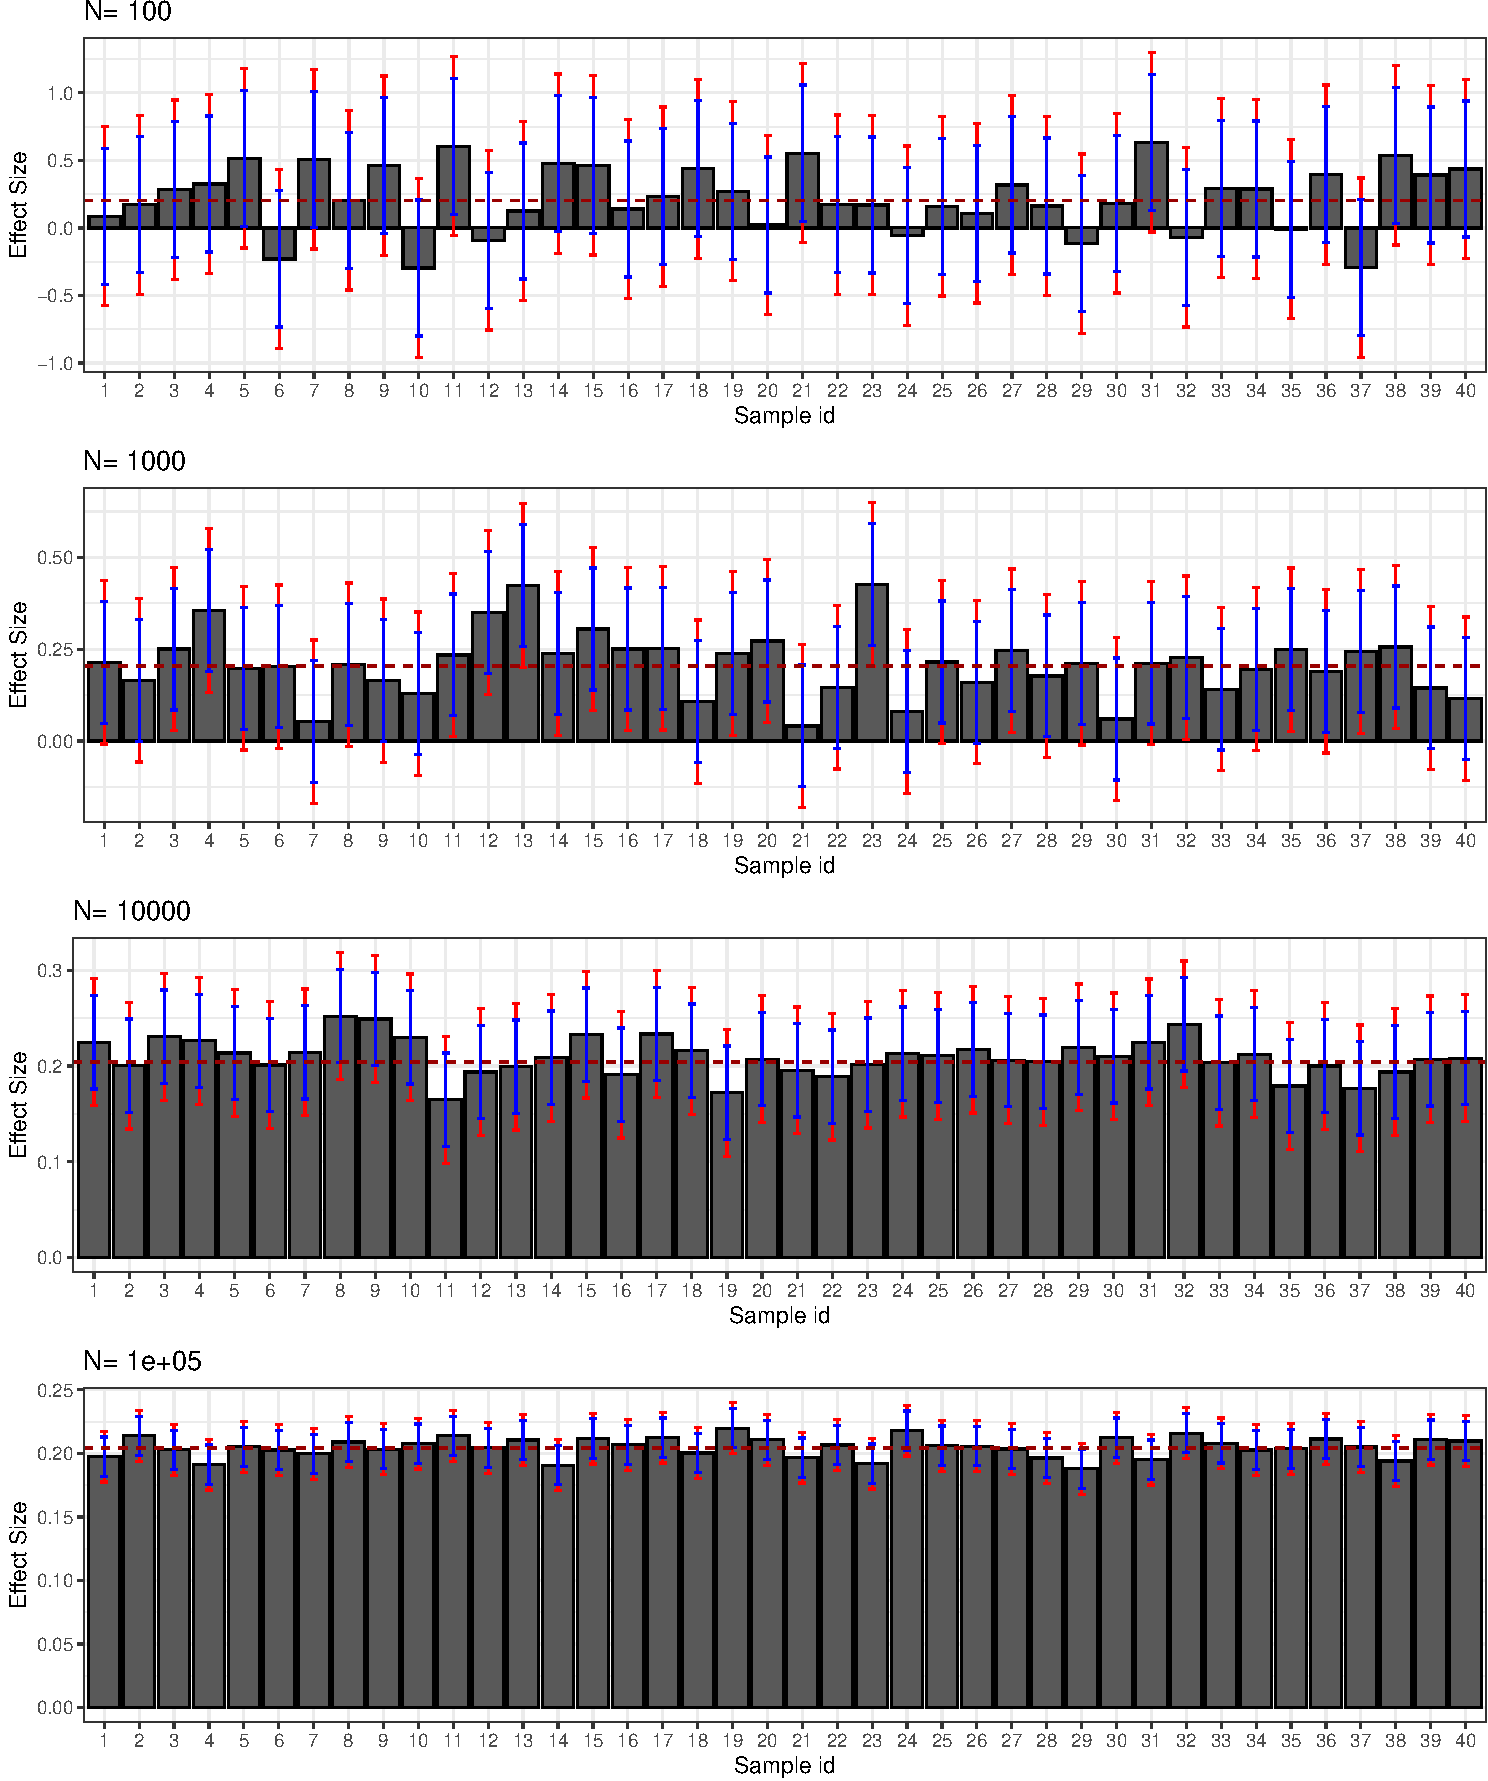
\includegraphics[width=0.6\linewidth]{STCI_files/figure-latex/confintervalES-1} 

}

\caption{Confidence intervals of $\hat{ES}$ for $\delta=$ 0.99 (red) and 0.95 (blue) over sample replications for various sample sizes}\label{fig:confintervalES}
\end{figure}

Figure \ref{fig:confintervalES} presents the 99\% and 95\% confidence
intervals for the effect size estimated in 40 samples selected from our
simulations. Let's regroup our estimate and see how we could present
their results.

\begin{Shaded}
\begin{Highlighting}[]
\NormalTok{test.all.ES <-}\StringTok{ }\KeywordTok{list}\NormalTok{()}
\ControlFlowTok{for}\NormalTok{ (k }\ControlFlowTok{in} \DecValTok{1}\OperatorTok{:}\KeywordTok{length}\NormalTok{(N.sample))\{}
  \KeywordTok{set.seed}\NormalTok{(}\DecValTok{1234}\NormalTok{)}
\NormalTok{  test.ES <-}\StringTok{ }\KeywordTok{sample}\NormalTok{(simuls.ww[[k]][,}\StringTok{'ES'}\NormalTok{],N.plot)}
\NormalTok{  test.ES <-}\StringTok{ }\KeywordTok{as.data.frame}\NormalTok{(}\KeywordTok{cbind}\NormalTok{(test.ES,}\KeywordTok{rep}\NormalTok{(}\KeywordTok{samp.noise.ES}\NormalTok{(simuls.ww[[k]][,}\StringTok{'ES'}\NormalTok{],}\DataTypeTok{delta=}\NormalTok{delta,}\DataTypeTok{param=}\NormalTok{param)),}\KeywordTok{rep}\NormalTok{(}\KeywordTok{samp.noise.ES}\NormalTok{(simuls.ww[[k]][,}\StringTok{'ES'}\NormalTok{],}\DataTypeTok{delta=}\NormalTok{delta.}\DecValTok{2}\NormalTok{,}\DataTypeTok{param=}\NormalTok{param))))}
  \KeywordTok{colnames}\NormalTok{(test.ES) <-}\StringTok{ }\KeywordTok{c}\NormalTok{(}\StringTok{'ES'}\NormalTok{,}\StringTok{'sampling.noise.ES.1'}\NormalTok{,}\StringTok{'sampling.noise.ES.2'}\NormalTok{)}
\NormalTok{  test.ES}\OperatorTok{$}\NormalTok{id <-}\StringTok{ }\DecValTok{1}\OperatorTok{:}\NormalTok{N.plot.ES}
\NormalTok{  test.all.ES[[k]] <-}\StringTok{ }\NormalTok{test.ES}
\NormalTok{\}}
\end{Highlighting}
\end{Shaded}

With \(N=\) 100, the reporting of the results for sample 1 would be
something like: ``we find an effect size of 0.09 \(\pm\) 0.66'' with
\(\delta=0,99\). With \(\delta=0.95\) we would say: ``we find an effect
of 0.09 \(\pm\) 0.5.'' All in all, our estimate is compatible with the
treatment having a large positive effect size and a medium negative
effect size. Low precision prevents us from saying much else.

With \(N=\) 1000, the reporting of the results for sample 1 with
\(\delta=0.99\) would be something like: ``we find an effect size of
0.21 \(\pm\) 0.22.'' With \(\delta=0.95\): ``we find an effect size of
0.21 \(\pm\) 0.17.'' Our estimate is compatible with a medium positive
effect or a very small positive or even negative effect (depending on
the choice of \(\delta\)).

With \(N=\) 10\^{}\{4\}, the reporting of the results for sample 1 with
\(\delta=0.99\) would be something like: ``we find an effect size of
0.22 \(\pm\) 0.07.'' With \(\delta=0.95\): ``we find an effect size of
0.22 \(\pm\) 0.05.'' Our estimate is thus compatible with a small effect
of the treatment. We can rule out that the effect of the treatment is
medium since the upper bound of the 99\% confidence interval is equal to
0.29. We can also rule out that the effect of the treatment is very
small since the lower bound of the 99\% confidence interval is equal to
0.16. With this sample size, we have been able to reach a precision
level sufficient enough to pin down the order of magnitude of the effect
size of our treatment. There still remains a considerable amount of
uncertainty about the true effect size, though: the upper bound of our
confidence interval is almost double the lower bound.

With \(N=\) 10\^{}\{5\}, the reporting of the results for sample 1 with
\(\delta=0.99\) would be something like: ``we find an effect size of 0.2
\(\pm\) 0.02.'' With \(\delta=0.95\): ``we find an effect size of 0.2
\(\pm\) 0.02.'' Here, the level of precision of our result is such that,
first, it does not depend on the choice of \(\delta\) in any meaningful
way, and second, we can do more than pinpoint the order of magnitude of
the effect size, we can start to zero in on its precise value. From our
estimate, the true value of the effect size is really close to 0.2. It
could be equal to 0.18 or 0.22, but not further away from 0.2 than that.
Remember that is actually equal to 0.2.

\BeginKnitrBlock{remark}
\iffalse{} {Remark. } \fi{}One issue with Cohen's \(d\) is that its
magnitude depends on the dispersion of the outcomes in the control
group. That means that for the same treatment, and same value of the
treatment effect, the effect size is larger in a population where
oucomes are more homogeneous. This is not an attractive feature of a
normalizing scale that its size depends on the particular application.
One solution would be, for each outcome, to provide a standardized
scale, using for example the estmated standard deviation in a reference
population. This would be similar to the invention of the metric system,
where a reference scale was agreed uppon once and for all.
\EndKnitrBlock{remark}

\BeginKnitrBlock{remark}
\iffalse{} {Remark. } \fi{}Cohen's \(d\) is well defined for continuous
outcomes. For discrete outcomes, the use of Cohen's \(d\) poses a series
of problems, and alternatives such as relative risk ratios and odds
ratios have been proposed. I'll comment on that in the last chapter.
\EndKnitrBlock{remark}

\section{Estimating sampling noise}\label{sec:estimsampnoise}

Gauging the extent sampling noise is very useful in order to be able to
determine how much we should trust our results. Are they precise, so
that the true treatment effect lies very close to our estimate? Or are
our results imprecise, the true treatment effect maybe lying very far
from our estimate?

Estimating sampling noise is hard because we want to infer a property of
our estimator over repeated samples using only one sample. In this
lecture, I am going to introduce four tools that enable you to gauge
sampling noise and to choose sample size. The four tools are Chebyshev's
inequality, the Central Limit Theorem, resampling methods and Fisher's
permutation method. The idea of all these methods is to use the
properties of the sample to infer the properties of our estimator over
replications. Chebyshev's inequality gives an upper bound on the
sampling noise and a lower bound on sample size, but these bounds are
generally too wide to be useful. The Central Limit Theorem (CLT)
approximates the distribution of \(\hat{E}\) by a normal distribution,
and quantifies sampling noise as a multiple of the standard deviation.
Resampling methods use the sample as a population and draw new samples
from it in order to approximate sampling noise. Fisher's permutation
method, also called randomization inference, derives the distribution of
\(\hat{E}\) under the assumption that all treatment effects are null, by
reallocating the treatment indicator among the treatment and control
group. Both the CLT and resampling methods are approximation methods,
and their approximation of the true extent of sampling noise gets better
and better as sample size increases. Fisher's permutation method is
exact-it is not an approximation-but it only works for the special case
of the \(WW\) estimator in a randomized design.

The remaining of this section is structured as follows. Section
\ref{sec:assumptions} introduces the assumptions that we will need in
order to implement the methods. Section \ref{sec:cheb} presents the
Chebyshev approach to gauging sampling noise and choosing sample size.
Section \ref{sec:CLT} introduces the CLT way of approximating sampling
noise and choosing sample size. Section \ref{sec:resamp} presents the
resampling methods.

\BeginKnitrBlock{remark}
\iffalse{} {Remark. } \fi{}I am going to derive the estimators for the
precision only for the \(WW\) estimator. In the following lectures, I
will show how these methods adapt to other estimators.
\EndKnitrBlock{remark}

\subsection{Assumptions}\label{sec:assumptions}

In order to be able to use the theorems that power up the methods that
we are going to use to gauge sampling noise, we need to make some
assumptions on the properties of the data. The main assumptions that we
need are that the estimator identifies the true effect of the treatment
in the population, that the estimator is well-defined in the sample,
that the observations in the sample are independently and identically
distributed (i.i.d.), that there is no interaction between units and
that the variances of the outcomes in the treated and untreated group
are finite.

We know from last lecture that for the \(WW\) estimator to identify
\(TT\), we need to assume that there is no selection bias, as stated in
Assumption \ref{def:noselb}. One way to ensure that this assumption
holds is to use a RCT.

In order to be able to form the \(WW\) estimator in the sample, we also
need that there is at least one treated and one untreated in the sample:

\BeginKnitrBlock{definition}[Full rank]
\protect\hypertarget{def:fullrank}{}{\label{def:fullrank} \iffalse (Full
rank) \fi{} }We assume that there is at least one observation in the
sample that receives the treatment and one observation that does not
receive it:

\begin{align*}
\exists i,j\leq N \text{ such that } & D_i=1 \& D_j=0.
\end{align*}
\EndKnitrBlock{definition}

One way to ensure that this assumption holds is to sample treated and
untreated units.

In order to be able to estimate the variance of the estimator easily, we
assume that the observations come from random sampling and are i.i.d.:

\BeginKnitrBlock{definition}[i.i.d. sampling]
\protect\hypertarget{def:iid}{}{\label{def:iid} \iffalse (i.i.d. sampling)
\fi{} }We assume that the observations in the sample are identically and
independently distributed:

\begin{align*}
\forall i,j\leq N\text{, }i\neq j\text{, } & (Y_i,D_i)\Ind(Y_j,D_j),\\
                                           & (Y_i,D_i)\&(Y_j,D_j)\sim F_{Y,D}.
\end{align*}
\EndKnitrBlock{definition}

We have to assume something on how the observations are related to each
other and to the population. Identical sampling is natural in the sense
that we are OK to assume that the observations stem from the same
population model. Independent sampling is something else altogether.
Independence means that the fates of two closely related individuals are
assumed to be independent. This rules out two empirically relevant
scenarios:

\begin{enumerate}
\def\labelenumi{\arabic{enumi}.}
\tightlist
\item
  The fates of individuals are related because of common influences, as
  for example the environment, etc,
\item
  The fates of individuals are related because they directly influence
  each other, as for example on a market, but also for example because
  there are diffusion effects, such as contagion of deseases or
  technological adoption by imitation.
\end{enumerate}

We will address both sources of failure of the independence assumption
in future lectures.

Finally, in order for all our derivations to make sense, we need to
assume that the outcomes in both groups have finite variances, otherwise
sampling noise is going to be too extreme to be able to estimate it
using the methods developed in this lecture:

\BeginKnitrBlock{definition}[Finite variance of $\hat{\Delta^Y_{WW}}$]
\protect\hypertarget{def:finitevar}{}{\label{def:finitevar} \iffalse (Finite
variance of \(\hat{\Delta^Y_{WW}}\)) \fi{} }We assume that
\(\var{Y^1|D_i=1}\) and \(\var{Y^0|D_i=0}\) are finite.
\EndKnitrBlock{definition}

\subsection{Using Chebyshev's inequality}\label{sec:cheb}

Chebyshev's inequality is a fundamental building block of statistics. It
relates the sampling noise of an estimator to its variance. More
precisely, it derives an upper bound on the samplig noise of an unbiased
estimator:

\BeginKnitrBlock{theorem}[Chebyshev's inequality]
\protect\hypertarget{thm:cheb}{}{\label{thm:cheb} \iffalse (Chebyshev's
inequality) \fi{} }For any unbiased estimator \(\hat{\theta}\), sampling
noise level \(2\epsilon\) and confidence level \(\delta\), sampling
noise is bounded from above:

\begin{align*}
2\epsilon \leq 2\sqrt{\frac{\var{\hat{\theta}}}{1-\delta}}.
\end{align*}
\EndKnitrBlock{theorem}

\BeginKnitrBlock{remark}
\iffalse{} {Remark. } \fi{}The more general version of Chebyshev's
inequality that is generally presented is as follows:

\begin{align*}
\Pr(|\hat{\theta}-\esp{\hat{\theta}}|>\epsilon) & \leq \frac{\var{\hat{\theta}}}{\epsilon^2}.
\end{align*}

The version I present in Theorem \ref{thm:cheb} is adapted to the
bouding of sampling noise for a given confidence level, while this
version is adapted to bounding the confidence level for a given level of
sampling noise. In order to go from this general version to Theorem
\ref{thm:cheb}, simply remember that, for an unbiased estimator,
\(\esp{\hat{\theta}}=\theta\) and that, by definition of sampling noise,
\(\Pr(|\hat{\theta}-\theta|>\epsilon)=1-\delta\). As a result,
\(1-\delta\leq\var{\hat{\theta}}/\epsilon^2\), hence the result in
Theorem \ref{thm:cheb}.
\EndKnitrBlock{remark}

Using Chebyshev's inequality, we can obtain an upper bound on the
sampling noise of the \(WW\) estimator:

\BeginKnitrBlock{theorem}[Upper bound on the sampling noise of $\hat{WW}$]
\protect\hypertarget{thm:uppsampnoise}{}{\label{thm:uppsampnoise}
\iffalse (Upper bound on the sampling noise of \(\hat{WW}\)) \fi{}
}Under Assumptions \ref{def:noselb}, \ref{def:fullrank} and
\ref{def:iid}, for a given confidence level \(\delta\), the sampling
noise of the \(\hat{WW}\) estimator is bounded from above:

\begin{align*}
2\epsilon \leq 2\sqrt{\frac{1}{N(1-\delta)}\left(\frac{\var{Y_i^1|D_i=1}}{\Pr(D_i=1)}+\frac{\var{Y_i^0|D_i=0}}{1-\Pr(D_i=1)}\right)}\equiv 2\bar{\epsilon}.
\end{align*}
\EndKnitrBlock{theorem}

\BeginKnitrBlock{proof}
\iffalse{} {Proof. } \fi{}See in Appendix \ref{proofcheb}
\EndKnitrBlock{proof}

Theorem \ref{thm:uppsampnoise} is a useful step forward for estimating
sampling noise. Theorem \ref{thm:uppsampnoise} states that the actual
level of sampling noise of the \(\hat{WW}\) estimator (\(2\epsilon\)) is
never bigger than a quantity that depends on sample size, confidence
level and on the variances of outcomes in the treated and control
groups. We either know all the components of the formula for
\(2\bar{\epsilon}\) or we can estimate them in the sample. For example,
\(\Pr(D_i=1)\), \(\var{Y_i^1|D_i=1}\) and \(\var{Y_i^0|D_i=0}\) by can
be approximated by, respectively:

\begin{align*}
  \hat{\Pr(D_i=1)} & = \frac{1}{N}\sum_{i=1}^ND_i\\
  \hat{\var{Y_i^1|D_i=1}} & = \frac{1}{\sum_{i=1}^ND_i}\sum_{i=1}^ND_i(Y_i-\frac{1}{\sum_{i=1}^ND_i}\sum_{i=1}^ND_iY_i)^2\\
  \hat{\var{Y_i^0|D_i=0}} & = \frac{1}{\sum_{i=1}^N(1-D_i)}\sum_{i=1}^N(1-D_i)(Y_i-\frac{1}{\sum_{i=1}^N(1-D_i)}\sum_{i=1}^N(1-D_i)Y_i)^2.
\end{align*}

Using these approximations for the quantities in the formula, we can
compute an estimate of the upper bound on sampling noise,
\(\hat{2\bar{\epsilon}}\).

\BeginKnitrBlock{example}
\protect\hypertarget{exm:unnamed-chunk-47}{}{\label{exm:unnamed-chunk-47}
}Let's write an R function that is going to compute an estimate for the
upper bound of sampling noise for any sample:
\EndKnitrBlock{example}

\begin{Shaded}
\begin{Highlighting}[]
\NormalTok{samp.noise.ww.cheb <-}\StringTok{ }\ControlFlowTok{function}\NormalTok{(N,delta,v1,v0,p)\{}
  \KeywordTok{return}\NormalTok{(}\DecValTok{2}\OperatorTok{*}\KeywordTok{sqrt}\NormalTok{((v1}\OperatorTok{/}\NormalTok{p}\OperatorTok{+}\NormalTok{v0}\OperatorTok{/}\NormalTok{(}\DecValTok{1}\OperatorTok{-}\NormalTok{p))}\OperatorTok{/}\NormalTok{(N}\OperatorTok{*}\NormalTok{(}\DecValTok{1}\OperatorTok{-}\NormalTok{delta))))}
\NormalTok{\}}
\end{Highlighting}
\end{Shaded}

Let's estimate this upper bound in our usual sample:

\begin{Shaded}
\begin{Highlighting}[]
\KeywordTok{set.seed}\NormalTok{(}\DecValTok{1234}\NormalTok{)}
\NormalTok{N <-}\DecValTok{1000}
\NormalTok{delta <-}\StringTok{ }\FloatTok{0.99}
\NormalTok{mu <-}\StringTok{ }\KeywordTok{rnorm}\NormalTok{(N,param[}\StringTok{"barmu"}\NormalTok{],}\KeywordTok{sqrt}\NormalTok{(param[}\StringTok{"sigma2mu"}\NormalTok{]))}
\NormalTok{UB <-}\StringTok{ }\KeywordTok{rnorm}\NormalTok{(N,}\DecValTok{0}\NormalTok{,}\KeywordTok{sqrt}\NormalTok{(param[}\StringTok{"sigma2U"}\NormalTok{]))}
\NormalTok{yB <-}\StringTok{ }\NormalTok{mu }\OperatorTok{+}\StringTok{ }\NormalTok{UB }
\NormalTok{YB <-}\StringTok{ }\KeywordTok{exp}\NormalTok{(yB)}
\NormalTok{Ds <-}\StringTok{ }\KeywordTok{rep}\NormalTok{(}\DecValTok{0}\NormalTok{,N)}
\NormalTok{V <-}\StringTok{ }\KeywordTok{rnorm}\NormalTok{(N,param[}\StringTok{"barmu"}\NormalTok{],}\KeywordTok{sqrt}\NormalTok{(param[}\StringTok{"sigma2mu"}\NormalTok{]}\OperatorTok{+}\NormalTok{param[}\StringTok{"sigma2U"}\NormalTok{]))}
\NormalTok{Ds[V}\OperatorTok{<=}\KeywordTok{log}\NormalTok{(param[}\StringTok{"barY"}\NormalTok{])] <-}\StringTok{ }\DecValTok{1} 
\NormalTok{epsilon <-}\StringTok{ }\KeywordTok{rnorm}\NormalTok{(N,}\DecValTok{0}\NormalTok{,}\KeywordTok{sqrt}\NormalTok{(param[}\StringTok{"sigma2epsilon"}\NormalTok{]))}
\NormalTok{eta<-}\StringTok{ }\KeywordTok{rnorm}\NormalTok{(N,}\DecValTok{0}\NormalTok{,}\KeywordTok{sqrt}\NormalTok{(param[}\StringTok{"sigma2eta"}\NormalTok{]))}
\NormalTok{U0 <-}\StringTok{ }\NormalTok{param[}\StringTok{"rho"}\NormalTok{]}\OperatorTok{*}\NormalTok{UB }\OperatorTok{+}\StringTok{ }\NormalTok{epsilon}
\NormalTok{y0 <-}\StringTok{ }\NormalTok{mu }\OperatorTok{+}\StringTok{  }\NormalTok{U0 }\OperatorTok{+}\StringTok{ }\NormalTok{param[}\StringTok{"delta"}\NormalTok{]}
\NormalTok{alpha <-}\StringTok{ }\NormalTok{param[}\StringTok{"baralpha"}\NormalTok{]}\OperatorTok{+}\StringTok{  }\NormalTok{param[}\StringTok{"theta"}\NormalTok{]}\OperatorTok{*}\NormalTok{mu }\OperatorTok{+}\StringTok{ }\NormalTok{eta}
\NormalTok{y1 <-}\StringTok{ }\NormalTok{y0}\OperatorTok{+}\NormalTok{alpha}
\NormalTok{Y0 <-}\StringTok{ }\KeywordTok{exp}\NormalTok{(y0)}
\NormalTok{Y1 <-}\StringTok{ }\KeywordTok{exp}\NormalTok{(y1)}
\NormalTok{y <-}\StringTok{ }\NormalTok{y1}\OperatorTok{*}\NormalTok{Ds}\OperatorTok{+}\NormalTok{y0}\OperatorTok{*}\NormalTok{(}\DecValTok{1}\OperatorTok{-}\NormalTok{Ds)}
\NormalTok{Y <-}\StringTok{ }\NormalTok{Y1}\OperatorTok{*}\NormalTok{Ds}\OperatorTok{+}\NormalTok{Y0}\OperatorTok{*}\NormalTok{(}\DecValTok{1}\OperatorTok{-}\NormalTok{Ds)}
\end{Highlighting}
\end{Shaded}

In our sample, for \(\delta=\) 0.99, \(\hat{2\bar{\epsilon}}=\) 1.35.
How does this compare with the true extent of sampling noise when \(N=\)
1000? Remember that we have computed an estimate of sampling noise out
of our Monte Carlo replications. In Table \ref{fig:precision}, we can
read that sampling noise is actually equal to 0.39. The Chebyshev upper
bound overestimates the extent of sampling noise by 245\%.

How does the Chebyshev upper bound fares overall? In order to know that,
let's compute the Chebyshev upper bound for all the simulated samples.
You might have noticed that, when running the Monte Carlo simulations
for the population parameter, I have not only recovered \(\hat{WW}\) for
each sample, but also the estimates of the components of the formula for
the upper bound on sampling noise. I can thus easily compute the
Chebyshev upper bound on sampling noise for each replication.

\begin{Shaded}
\begin{Highlighting}[]
\ControlFlowTok{for}\NormalTok{ (k }\ControlFlowTok{in}\NormalTok{ (}\DecValTok{1}\OperatorTok{:}\KeywordTok{length}\NormalTok{(N.sample)))\{}
\NormalTok{  simuls.ww[[k]]}\OperatorTok{$}\NormalTok{cheb.noise <-}\StringTok{ }\KeywordTok{samp.noise.ww.cheb}\NormalTok{(N.sample[[k]],delta,simuls.ww[[k]][,}\StringTok{'V1'}\NormalTok{],simuls.ww[[k]][,}\StringTok{'V0'}\NormalTok{],simuls.ww[[k]][,}\StringTok{'p'}\NormalTok{])}
\NormalTok{\}}
\KeywordTok{par}\NormalTok{(}\DataTypeTok{mfrow=}\KeywordTok{c}\NormalTok{(}\DecValTok{2}\NormalTok{,}\DecValTok{2}\NormalTok{))}
\ControlFlowTok{for}\NormalTok{ (i }\ControlFlowTok{in} \DecValTok{1}\OperatorTok{:}\DecValTok{4}\NormalTok{)\{}
  \KeywordTok{hist}\NormalTok{(simuls.ww[[i]][,}\StringTok{'cheb.noise'}\NormalTok{],}\DataTypeTok{main=}\KeywordTok{paste}\NormalTok{(}\StringTok{'N='}\NormalTok{,}\KeywordTok{as.character}\NormalTok{(N.sample[i])),}\DataTypeTok{xlab=}\KeywordTok{expression}\NormalTok{(}\KeywordTok{hat}\NormalTok{(}\DecValTok{2}\OperatorTok{*}\KeywordTok{bar}\NormalTok{(epsilon))),}\DataTypeTok{xlim=}\KeywordTok{c}\NormalTok{(}\FloatTok{0.25}\OperatorTok{*}\KeywordTok{min}\NormalTok{(simuls.ww[[i]][,}\StringTok{'cheb.noise'}\NormalTok{]),}\KeywordTok{max}\NormalTok{(simuls.ww[[i]][,}\StringTok{'cheb.noise'}\NormalTok{])))}
  \KeywordTok{abline}\NormalTok{(}\DataTypeTok{v=}\NormalTok{table.noise[i,}\KeywordTok{colnames}\NormalTok{(table.noise)}\OperatorTok{==}\StringTok{'sampling.noise'}\NormalTok{],}\DataTypeTok{col=}\StringTok{"red"}\NormalTok{)}
\NormalTok{\}}
\end{Highlighting}
\end{Shaded}

\begin{figure}[htbp]

{\centering 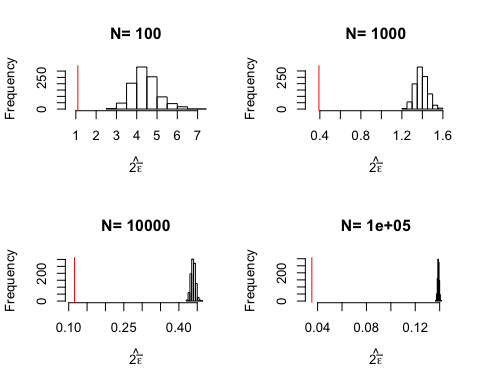
\includegraphics[width=0.6\linewidth]{STCI_files/figure-latex/sampnoisewwcheball-1} 

}

\caption{Distribution of the Chebyshev upper bound on sampling noise over replications of samples of different sizes (true sampling noise in red)}\label{fig:sampnoisewwcheball}
\end{figure}

Figure \ref{fig:sampnoisewwcheball} shows that the upper bound works: it
is always bigger than the true sampling noise. Figure
\ref{fig:sampnoisewwcheball} also shows that the upper bound is large:
it generally is of an order of magnitude bigger than the true sampling
noise, and thus offers a blurry and too pessimistic view of the
precision of an estimator. Figure \ref{fig:sampnoisewwchebplot} shows
that the average Chebyshev bound gives an inflated estimate of sampling
noise. Figure \ref{fig:confintervalcheb} shows that the Chebyshev
confidence intervals are clearly less precise than the true unknown
ones. With \(N=\) 1000, the true confidence intervals generally reject
large negative effects, whereas the Chebyshev confidence intervals do
not rule out this possibility. With \(N=\) 10\^{}\{4\}, the true
confidence intervals generally reject effects smaller than 0.1, whereas
the Chebyshev confidence intervals cannot rule out small negative
effects.

As a conclusion on Chebyshev estimates of sampling noise, their
advantage is that they offer an upper bound on the noise: we can never
underestimate noise if we use them. A downside of Chebyshev sampling
noise estimates is their low precision, which makes it hard to pinpoint
the true confidence intervals.

\begin{Shaded}
\begin{Highlighting}[]
\ControlFlowTok{for}\NormalTok{ (k }\ControlFlowTok{in}\NormalTok{ (}\DecValTok{1}\OperatorTok{:}\KeywordTok{length}\NormalTok{(N.sample)))\{}
\NormalTok{  table.noise}\OperatorTok{$}\NormalTok{cheb.noise[k] <-}\StringTok{ }\KeywordTok{mean}\NormalTok{(simuls.ww[[k]]}\OperatorTok{$}\NormalTok{cheb.noise)}
\NormalTok{\}}
\KeywordTok{ggplot}\NormalTok{(table.noise, }\KeywordTok{aes}\NormalTok{(}\DataTypeTok{x=}\KeywordTok{as.factor}\NormalTok{(N), }\DataTypeTok{y=}\NormalTok{TT)) }\OperatorTok{+}
\StringTok{  }\KeywordTok{geom_bar}\NormalTok{(}\DataTypeTok{position=}\KeywordTok{position_dodge}\NormalTok{(), }\DataTypeTok{stat=}\StringTok{"identity"}\NormalTok{, }\DataTypeTok{colour=}\StringTok{'black'}\NormalTok{) }\OperatorTok{+}
\StringTok{  }\KeywordTok{geom_errorbar}\NormalTok{(}\KeywordTok{aes}\NormalTok{(}\DataTypeTok{ymin=}\NormalTok{TT}\OperatorTok{-}\NormalTok{sampling.noise}\OperatorTok{/}\DecValTok{2}\NormalTok{, }\DataTypeTok{ymax=}\NormalTok{TT}\OperatorTok{+}\NormalTok{sampling.noise}\OperatorTok{/}\DecValTok{2}\NormalTok{), }\DataTypeTok{width=}\NormalTok{.}\DecValTok{2}\NormalTok{,}\DataTypeTok{position=}\KeywordTok{position_dodge}\NormalTok{(.}\DecValTok{9}\NormalTok{),}\DataTypeTok{color=}\StringTok{'red'}\NormalTok{) }\OperatorTok{+}
\StringTok{  }\KeywordTok{geom_errorbar}\NormalTok{(}\KeywordTok{aes}\NormalTok{(}\DataTypeTok{ymin=}\NormalTok{TT}\OperatorTok{-}\NormalTok{cheb.noise}\OperatorTok{/}\DecValTok{2}\NormalTok{, }\DataTypeTok{ymax=}\NormalTok{TT}\OperatorTok{+}\NormalTok{cheb.noise}\OperatorTok{/}\DecValTok{2}\NormalTok{), }\DataTypeTok{width=}\NormalTok{.}\DecValTok{2}\NormalTok{,}\DataTypeTok{position=}\KeywordTok{position_dodge}\NormalTok{(.}\DecValTok{9}\NormalTok{),}\DataTypeTok{color=}\StringTok{'blue'}\NormalTok{) }\OperatorTok{+}
\StringTok{  }\KeywordTok{xlab}\NormalTok{(}\StringTok{"Sample Size"}\NormalTok{)}\OperatorTok{+}
\StringTok{  }\KeywordTok{theme_bw}\NormalTok{()}
\end{Highlighting}
\end{Shaded}

\begin{figure}[htbp]

{\centering 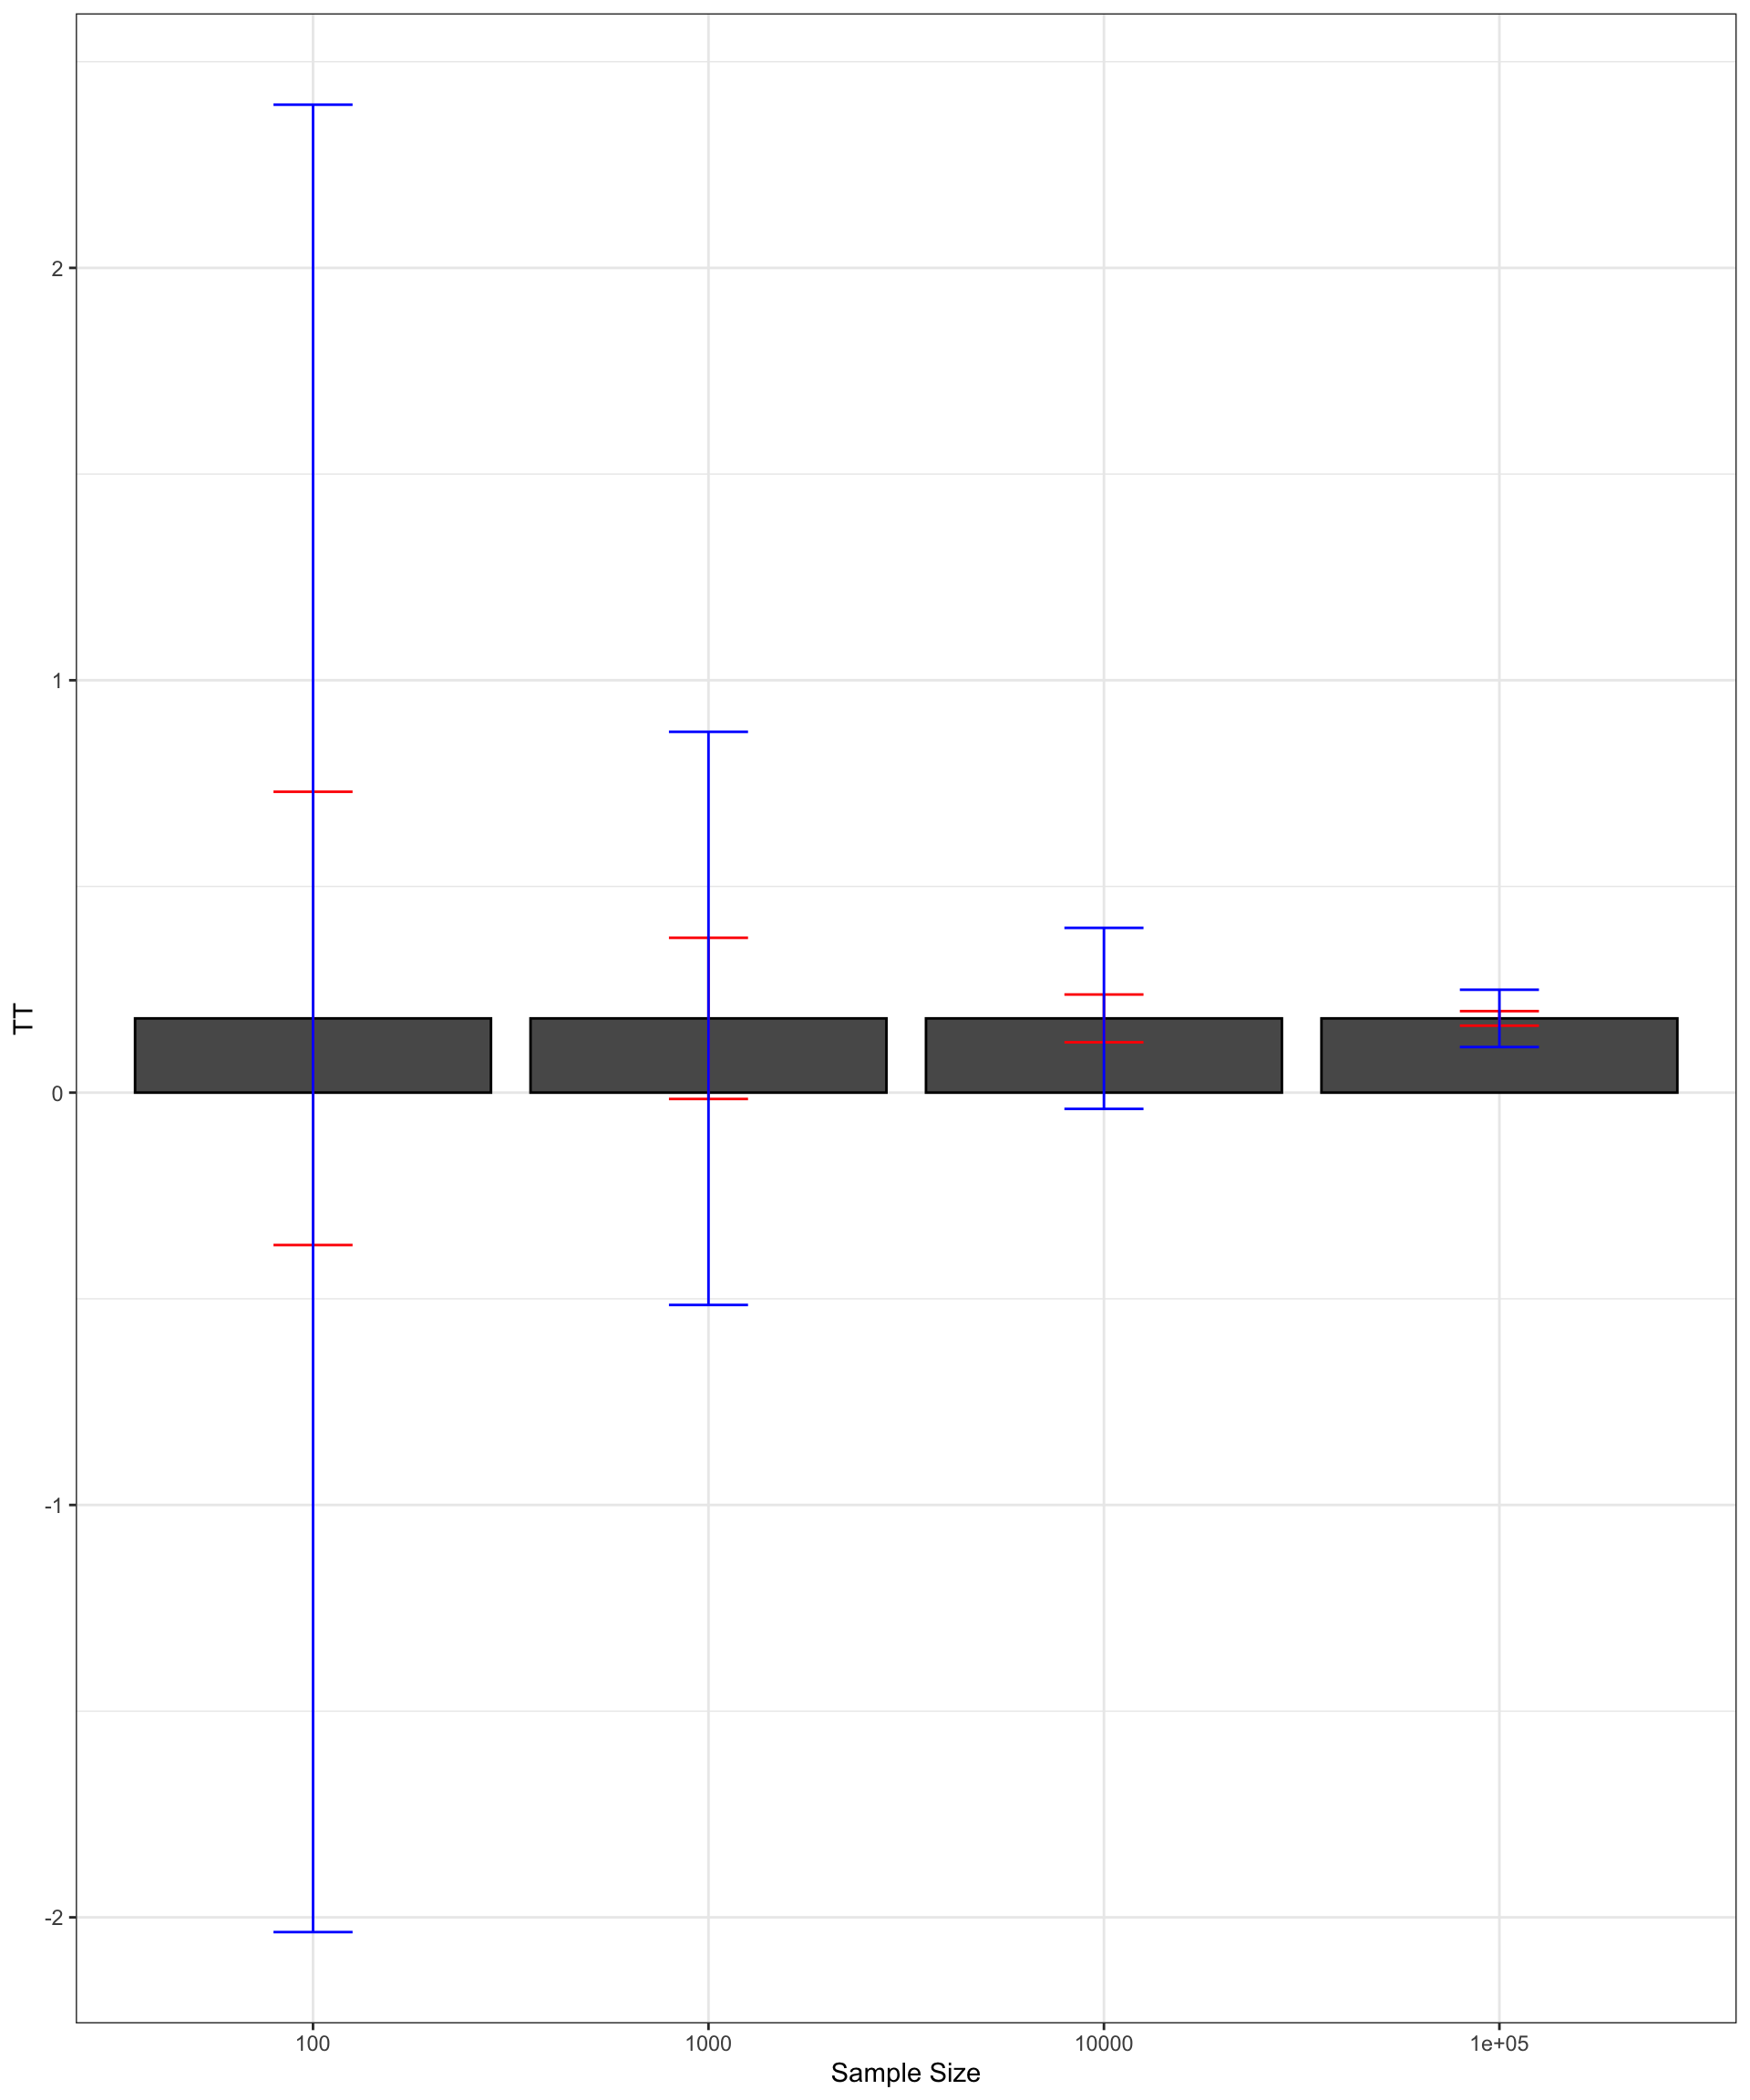
\includegraphics[width=0.6\linewidth]{STCI_files/figure-latex/sampnoisewwchebplot-1} 

}

\caption{Average Chebyshev upper bound on sampling noise over replications of samples of different sizes (true sampling noise in red)}\label{fig:sampnoisewwchebplot}
\end{figure}

\begin{Shaded}
\begin{Highlighting}[]
\NormalTok{N.plot <-}\StringTok{ }\DecValTok{40}
\NormalTok{plot.list <-}\StringTok{ }\KeywordTok{list}\NormalTok{()}

\ControlFlowTok{for}\NormalTok{ (k }\ControlFlowTok{in} \DecValTok{1}\OperatorTok{:}\KeywordTok{length}\NormalTok{(N.sample))\{}
  \KeywordTok{set.seed}\NormalTok{(}\DecValTok{1234}\NormalTok{)}
\NormalTok{  test.cheb <-}\StringTok{ }\NormalTok{simuls.ww[[k]][}\KeywordTok{sample}\NormalTok{(N.plot),}\KeywordTok{c}\NormalTok{(}\StringTok{'WW'}\NormalTok{,}\StringTok{'cheb.noise'}\NormalTok{)]}
\NormalTok{  test.cheb <-}\StringTok{ }\KeywordTok{as.data.frame}\NormalTok{(}\KeywordTok{cbind}\NormalTok{(test.cheb,}\KeywordTok{rep}\NormalTok{(}\KeywordTok{samp.noise}\NormalTok{(simuls.ww[[k]][,}\StringTok{'WW'}\NormalTok{],}\DataTypeTok{delta=}\NormalTok{delta),N.plot)))}
  \KeywordTok{colnames}\NormalTok{(test.cheb) <-}\StringTok{ }\KeywordTok{c}\NormalTok{(}\StringTok{'WW'}\NormalTok{,}\StringTok{'cheb.noise'}\NormalTok{,}\StringTok{'sampling.noise'}\NormalTok{)}
\NormalTok{  test.cheb}\OperatorTok{$}\NormalTok{id <-}\StringTok{ }\DecValTok{1}\OperatorTok{:}\NormalTok{N.plot}
\NormalTok{  plot.test.cheb <-}\StringTok{ }\KeywordTok{ggplot}\NormalTok{(test.cheb, }\KeywordTok{aes}\NormalTok{(}\DataTypeTok{x=}\KeywordTok{as.factor}\NormalTok{(id), }\DataTypeTok{y=}\NormalTok{WW)) }\OperatorTok{+}
\StringTok{      }\KeywordTok{geom_bar}\NormalTok{(}\DataTypeTok{position=}\KeywordTok{position_dodge}\NormalTok{(), }\DataTypeTok{stat=}\StringTok{"identity"}\NormalTok{, }\DataTypeTok{colour=}\StringTok{'black'}\NormalTok{) }\OperatorTok{+}
\StringTok{      }\KeywordTok{geom_errorbar}\NormalTok{(}\KeywordTok{aes}\NormalTok{(}\DataTypeTok{ymin=}\NormalTok{WW}\OperatorTok{-}\NormalTok{sampling.noise}\OperatorTok{/}\DecValTok{2}\NormalTok{, }\DataTypeTok{ymax=}\NormalTok{WW}\OperatorTok{+}\NormalTok{sampling.noise}\OperatorTok{/}\DecValTok{2}\NormalTok{), }\DataTypeTok{width=}\NormalTok{.}\DecValTok{2}\NormalTok{,}\DataTypeTok{position=}\KeywordTok{position_dodge}\NormalTok{(.}\DecValTok{9}\NormalTok{),}\DataTypeTok{color=}\StringTok{'red'}\NormalTok{) }\OperatorTok{+}
\StringTok{      }\KeywordTok{geom_errorbar}\NormalTok{(}\KeywordTok{aes}\NormalTok{(}\DataTypeTok{ymin=}\NormalTok{WW}\OperatorTok{-}\NormalTok{cheb.noise}\OperatorTok{/}\DecValTok{2}\NormalTok{, }\DataTypeTok{ymax=}\NormalTok{WW}\OperatorTok{+}\NormalTok{cheb.noise}\OperatorTok{/}\DecValTok{2}\NormalTok{), }\DataTypeTok{width=}\NormalTok{.}\DecValTok{2}\NormalTok{,}\DataTypeTok{position=}\KeywordTok{position_dodge}\NormalTok{(.}\DecValTok{9}\NormalTok{),}\DataTypeTok{color=}\StringTok{'blue'}\NormalTok{) }\OperatorTok{+}
\StringTok{      }\KeywordTok{geom_hline}\NormalTok{(}\KeywordTok{aes}\NormalTok{(}\DataTypeTok{yintercept=}\KeywordTok{delta.y.ate}\NormalTok{(param)), }\DataTypeTok{colour=}\StringTok{"#990000"}\NormalTok{, }\DataTypeTok{linetype=}\StringTok{"dashed"}\NormalTok{)}\OperatorTok{+}
\StringTok{      }\KeywordTok{xlab}\NormalTok{(}\StringTok{"Sample id"}\NormalTok{)}\OperatorTok{+}
\StringTok{      }\KeywordTok{theme_bw}\NormalTok{()}\OperatorTok{+}
\StringTok{      }\KeywordTok{ggtitle}\NormalTok{(}\KeywordTok{paste}\NormalTok{(}\StringTok{"N="}\NormalTok{,N.sample[k]))}
\NormalTok{  plot.list[[k]] <-}\StringTok{ }\NormalTok{plot.test.cheb }
\NormalTok{\}}
\NormalTok{plot.CI <-}\StringTok{ }\KeywordTok{plot_grid}\NormalTok{(plot.list[[}\DecValTok{1}\NormalTok{]],plot.list[[}\DecValTok{2}\NormalTok{]],plot.list[[}\DecValTok{3}\NormalTok{]],plot.list[[}\DecValTok{4}\NormalTok{]],}\DataTypeTok{ncol=}\DecValTok{1}\NormalTok{,}\DataTypeTok{nrow=}\KeywordTok{length}\NormalTok{(N.sample))}
\KeywordTok{print}\NormalTok{(plot.CI)}
\end{Highlighting}
\end{Shaded}

\begin{figure}[htbp]

{\centering 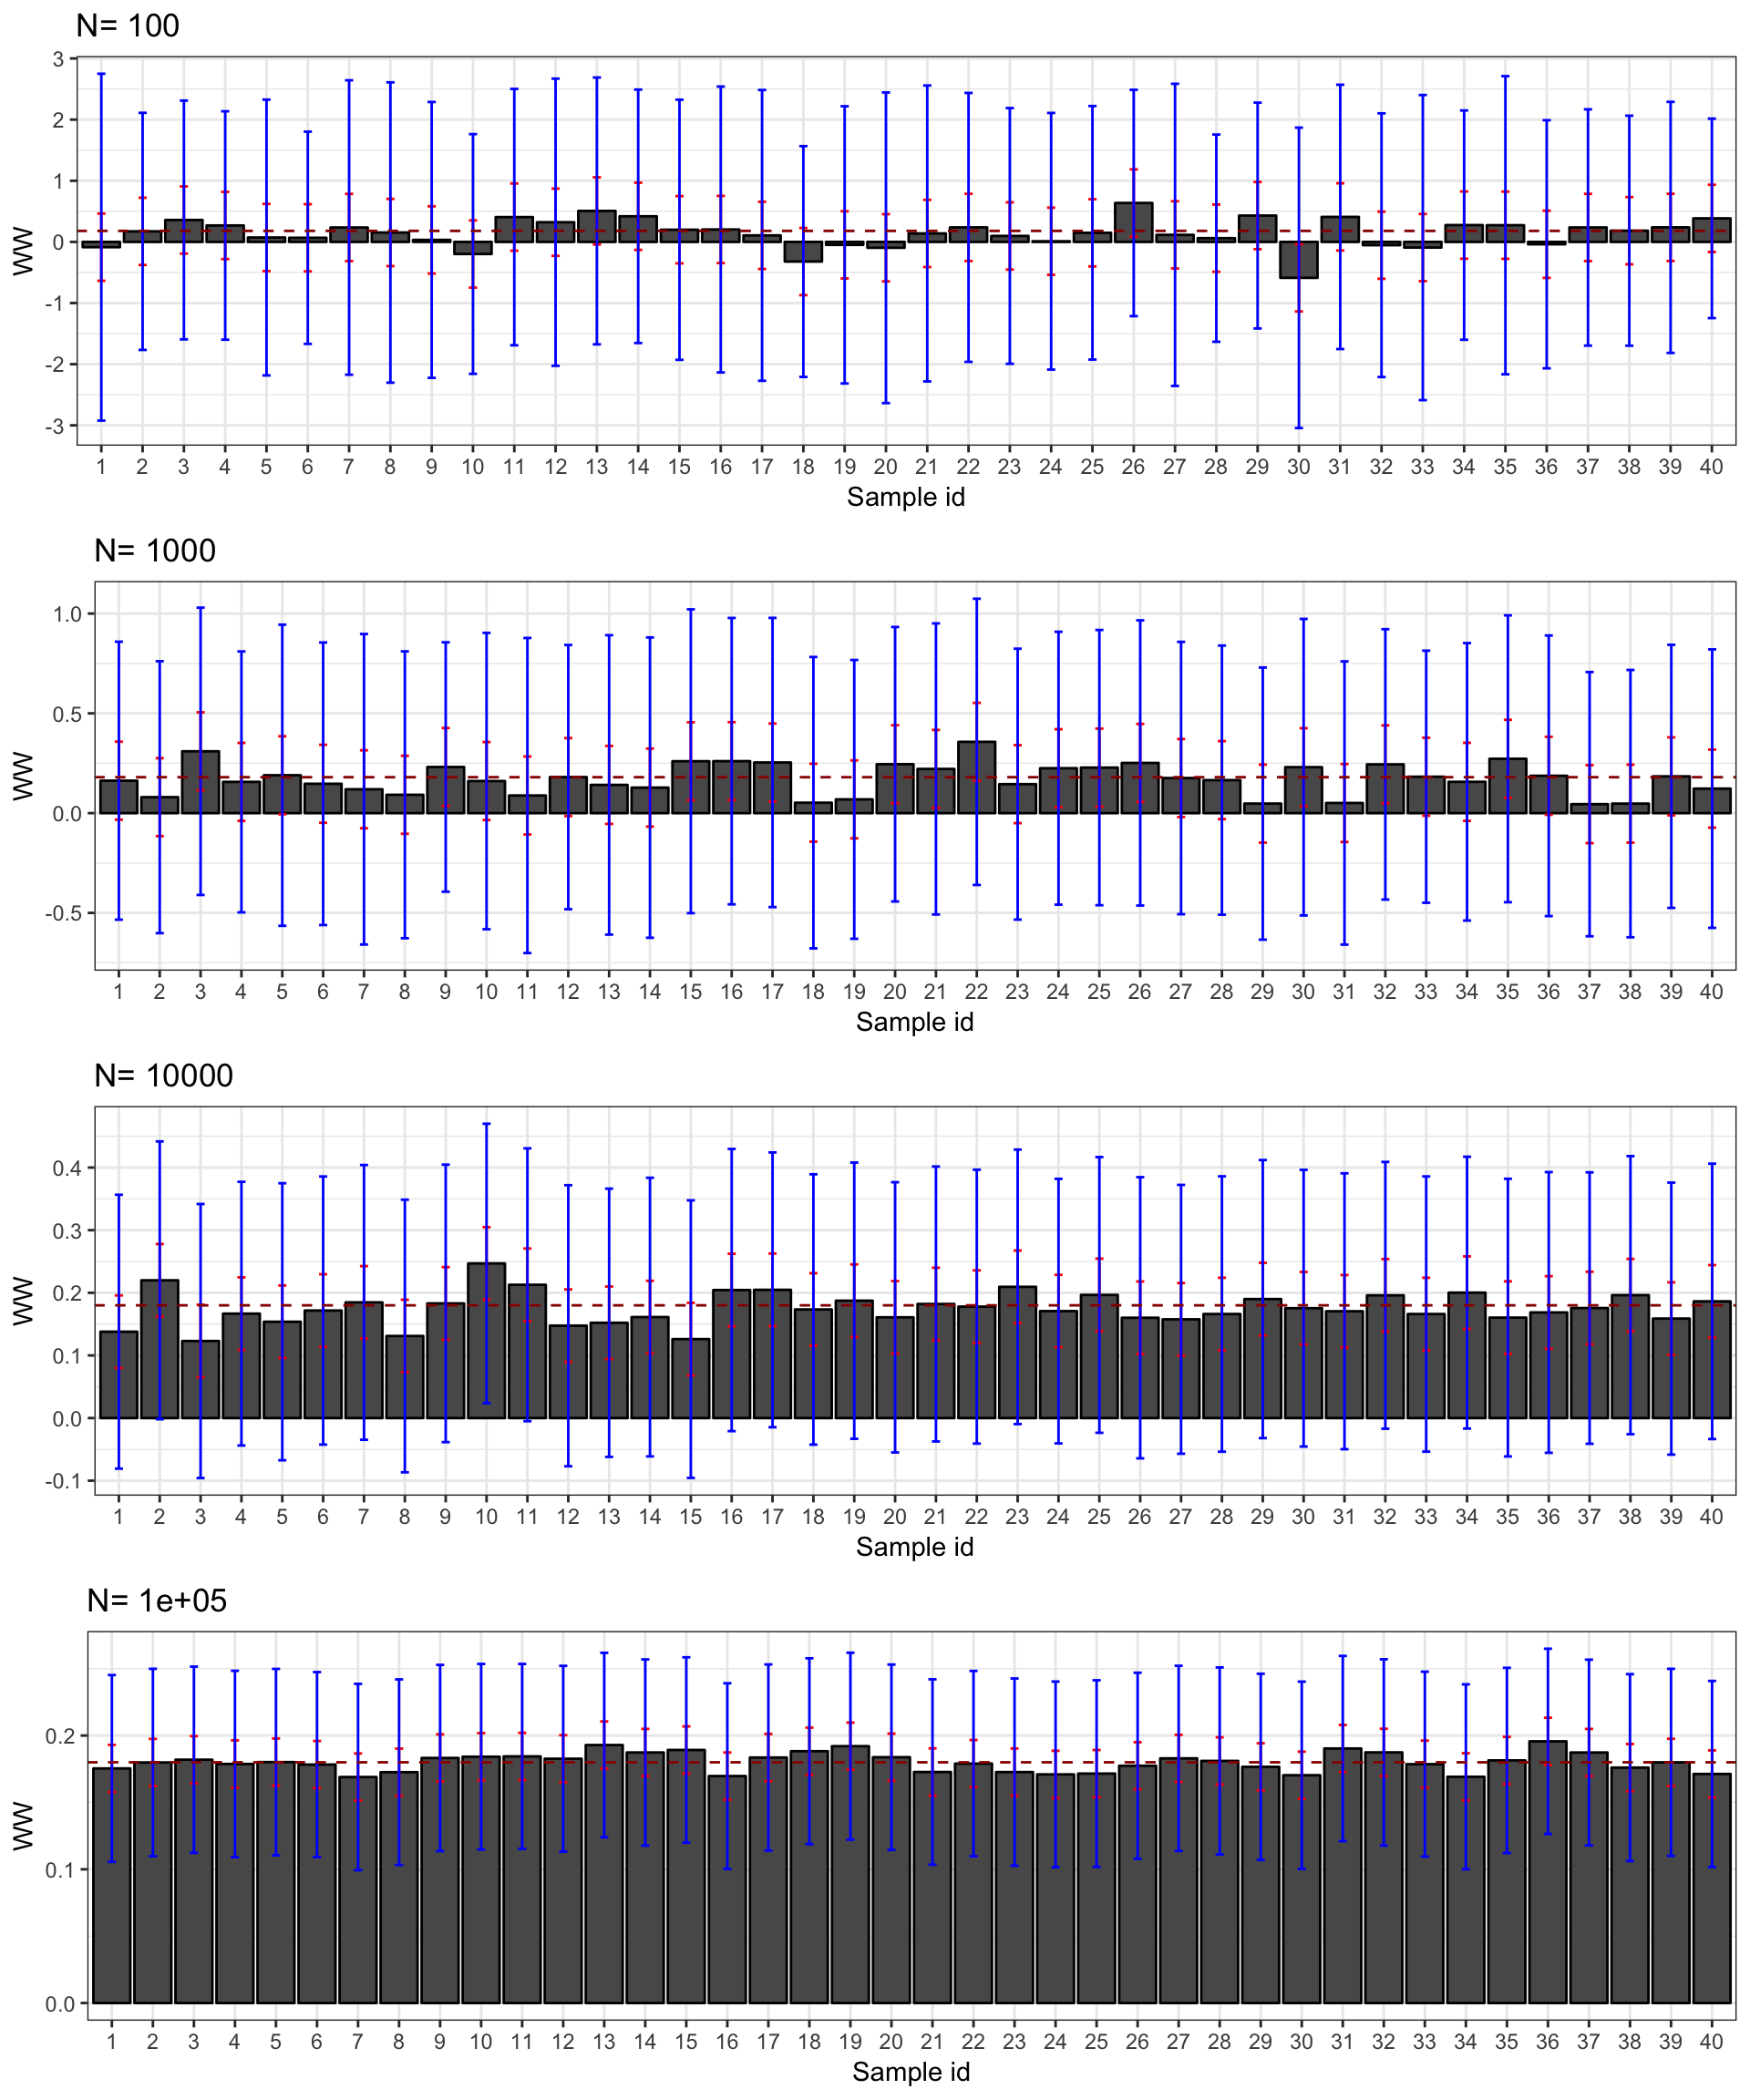
\includegraphics[width=0.6\linewidth]{STCI_files/figure-latex/confintervalcheb-1} 

}

\caption{Chebyshev confidence intervals of $\hat{WW}$ for $\delta=$ 0.99 over sample replications for various sample sizes (true confidence intervals in red)}\label{fig:confintervalcheb}
\end{figure}

\subsection{Using the Central Limit Theorem}\label{sec:CLT}

The main problem with Chebyshev's upper bound on sampling noise is that
it is an upper bound, and thus it overestimates sampling noise and
underestimates precision. One alternative to using Chebyshev's upper
bound is to use the Central Limit Theorem (CLT). In econometrics and
statistics, the CLT is used to derive approximate values for the
sampling noise of estimators. Because these approximations become more
and more precise as sample size increases, we call them asymptotic
approximations.

Taken to its bare bones, the CLT states that the sum of i.i.d. random
variables behaves approximately like a normal distribution when the
sample size is large:

\BeginKnitrBlock{theorem}[Central Limit Theorem]
\protect\hypertarget{thm:CLT}{}{\label{thm:CLT} \iffalse (Central Limit
Theorem) \fi{} }Let \(X_i\) be i.i.d. random variables with
\(\esp{X_i}=\mu\) and \(\var{X_i}=\sigma^2\), and define
\(Z_N=\frac{\frac{1}{N}\sum_{i=1}^NX_i-\mu}{\frac{\sigma}{\sqrt{N}}}\),
then, for all \(z\) we have:

\begin{align*}
\lim_{N\rightarrow\infty}\Pr(Z_N\leq z) & = \Phi(z),
\end{align*}

where \(\Phi\) is the cumulative distribution function of the centered
standardized normal.

We say that \(Z_N\) converges in distribution to a standard normal
random variable, and we denote:
\(Z_N\stackrel{d}{\rightarrow}\mathcal{N}(0,1)\).
\EndKnitrBlock{theorem}

The CLT is a beautiful result: the distribution of the average of
realisations of any random variable that has finite mean and variance
can be approximated by a normal when the sample size is large enough.
The CLT is somehow limited though because not all estimators are sums.
Estimators are generally more or less complex combinations of sums. In
order to derive the asymptotic approximation for a lot of estimators
that are combinations of sums, econometricians and statisticians
complement the CLT with two other extremely powerful tools: Slutsky's
theorem and the Delta method. Slutsky's theorem states that sums,
products and ratios of sums that converge to a normal converge to the
sum, product or ratio of these normals. The Delta method states that a
function of a sum that converges to a normal converges to a normal whose
variance is a quadratic form of the variance of the sum and of the first
derivative of the function. Both of these tools are stated more
rigorously in the appendix, but you do not need to know them for this
class. The idea is for you to be aware of how the main approximations
that we are going to use throughout this class have been derived.

Let me now state the main result of this section:

\BeginKnitrBlock{theorem}[Asymptotic Estimate of Sampling Noise of WW]
\protect\hypertarget{thm:asympnoiseWW}{}{\label{thm:asympnoiseWW}
\iffalse (Asymptotic Estimate of Sampling Noise of WW) \fi{} }Under
Assumptions \ref{def:noselb}, \ref{def:fullrank}, \ref{def:iid} and
\ref{def:finitevar}, for a given confidence level \(\delta\) and sample
size \(N\), the sampling noise of \(\hat{WW}\) can be approximated as
follows:

\begin{align*}
2\epsilon & \approx 2\Phi^{-1}\left(\frac{\delta+1}{2}\right)\frac{1}{\sqrt{N}}\sqrt{\frac{\var{Y_i^1|D_i=1}}{\Pr(D_i=1)}+\frac{\var{Y_i^0|D_i=0}}{1-\Pr(D_i=1)}} \equiv 2\tilde{\epsilon}.
\end{align*}
\EndKnitrBlock{theorem}

\BeginKnitrBlock{proof}
\iffalse{} {Proof. } \fi{}See in Appendix \ref{proofCLT}.
\EndKnitrBlock{proof}

Let's write an R function that computes this formula:

\begin{Shaded}
\begin{Highlighting}[]
\NormalTok{samp.noise.ww.CLT <-}\StringTok{ }\ControlFlowTok{function}\NormalTok{(N,delta,v1,v0,p)\{}
  \KeywordTok{return}\NormalTok{(}\DecValTok{2}\OperatorTok{*}\KeywordTok{qnorm}\NormalTok{((delta}\OperatorTok{+}\DecValTok{1}\NormalTok{)}\OperatorTok{/}\DecValTok{2}\NormalTok{)}\OperatorTok{*}\KeywordTok{sqrt}\NormalTok{((v1}\OperatorTok{/}\NormalTok{p}\OperatorTok{+}\NormalTok{v0}\OperatorTok{/}\NormalTok{(}\DecValTok{1}\OperatorTok{-}\NormalTok{p))}\OperatorTok{/}\NormalTok{N))}
\NormalTok{\}}
\end{Highlighting}
\end{Shaded}

\BeginKnitrBlock{example}
\protect\hypertarget{exm:unnamed-chunk-49}{}{\label{exm:unnamed-chunk-49}
}Let's see how the CLT performs in our example.
\EndKnitrBlock{example} In our sample, for \(\delta=\) 0.99, the CLT
estimate of sampling noise is \(\hat{2\tilde{\epsilon}}=\) 0.35. How
does this compare with the true extent of sampling noise when \(N=\)
1000? Remember that we have computed an estimate of sampling noise out
of our Monte Carlo replications. In Table \ref{tab:precisionsignal}, we
can read that sampling noise is actually equal to 0.39. The CLT
approximation is pretty precise: it only underestimates the true extent
of sampling noise by 11\%.

We can also compute the CLT approximation to sampling noise in all of
our samples:

\begin{Shaded}
\begin{Highlighting}[]
\ControlFlowTok{for}\NormalTok{ (k }\ControlFlowTok{in}\NormalTok{ (}\DecValTok{1}\OperatorTok{:}\KeywordTok{length}\NormalTok{(N.sample)))\{}
\NormalTok{  simuls.ww[[k]]}\OperatorTok{$}\NormalTok{CLT.noise <-}\StringTok{ }\KeywordTok{samp.noise.ww.CLT}\NormalTok{(N.sample[[k]],delta,simuls.ww[[k]][,}\StringTok{'V1'}\NormalTok{],simuls.ww[[k]][,}\StringTok{'V0'}\NormalTok{],simuls.ww[[k]][,}\StringTok{'p'}\NormalTok{])}
\NormalTok{\}}
\KeywordTok{par}\NormalTok{(}\DataTypeTok{mfrow=}\KeywordTok{c}\NormalTok{(}\DecValTok{2}\NormalTok{,}\DecValTok{2}\NormalTok{))}
\ControlFlowTok{for}\NormalTok{ (i }\ControlFlowTok{in} \DecValTok{1}\OperatorTok{:}\DecValTok{4}\NormalTok{)\{}
  \KeywordTok{hist}\NormalTok{(simuls.ww[[i]][,}\StringTok{'CLT.noise'}\NormalTok{],}\DataTypeTok{main=}\KeywordTok{paste}\NormalTok{(}\StringTok{'N='}\NormalTok{,}\KeywordTok{as.character}\NormalTok{(N.sample[i])),}\DataTypeTok{xlab=}\KeywordTok{expression}\NormalTok{(}\KeywordTok{hat}\NormalTok{(}\DecValTok{2}\OperatorTok{*}\KeywordTok{bar}\NormalTok{(epsilon))),}\DataTypeTok{xlim=}\KeywordTok{c}\NormalTok{(}\KeywordTok{min}\NormalTok{(simuls.ww[[i]][,}\StringTok{'CLT.noise'}\NormalTok{]),}\KeywordTok{max}\NormalTok{(simuls.ww[[i]][,}\StringTok{'CLT.noise'}\NormalTok{])))}
  \KeywordTok{abline}\NormalTok{(}\DataTypeTok{v=}\NormalTok{table.noise[i,}\KeywordTok{colnames}\NormalTok{(table.noise)}\OperatorTok{==}\StringTok{'sampling.noise'}\NormalTok{],}\DataTypeTok{col=}\StringTok{"red"}\NormalTok{)}
\NormalTok{\}}
\end{Highlighting}
\end{Shaded}

\begin{figure}[htbp]

{\centering 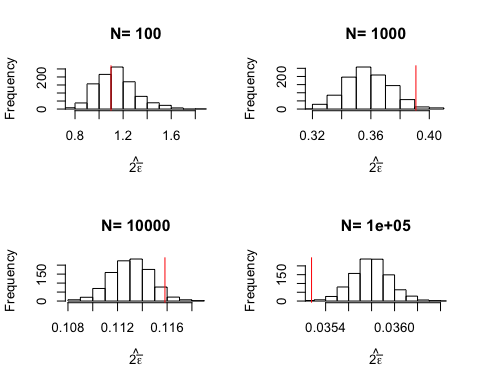
\includegraphics[width=0.6\linewidth]{STCI_files/figure-latex/sampnoisewwCLTall-1} 

}

\caption{Distribution of the CLT approximation of sampling noise over replications of samples of different sizes (true sampling noise in red)}\label{fig:sampnoisewwCLTall}
\end{figure}

Figure \ref{fig:sampnoisewwCLTall} shows that the CLT works: CLT-based
estimates of sampling noise approximates true sampling noise well.
CLT-based approximations of sampling noise are even impressively
accurate: they always capture the exact order of magnitude of sampling
noise, although there is a slight underestimation when \(N=\) 1000 and
10\^{}\{4\} and a slight overestimation when \(N=\) 10\^{}\{5\}. This
success should not come as a surprise as all shocks in our model are
normally distributed, meaning that the CLT results are more than an
approximation, they are exact. Results might be less spectacular when
estimating the effect of the treatment on the outcomes in levels rather
than in logs.

As a consequence, the average CLT-based estimates of sampling noise and
of confidence intervals are pretty precise, as Figures
\ref{fig:sampnoisewwCLTplot} and \ref{fig:confintervalCLT} show. Let's
pause for a second at the beauty of what we have achieved using the CLT:
by using only information from one sample, we have been able to gauge
extremely precisely how the estimator would behave over sampling
repetitions.

\begin{Shaded}
\begin{Highlighting}[]
\ControlFlowTok{for}\NormalTok{ (k }\ControlFlowTok{in}\NormalTok{ (}\DecValTok{1}\OperatorTok{:}\KeywordTok{length}\NormalTok{(N.sample)))\{}
\NormalTok{  table.noise}\OperatorTok{$}\NormalTok{CLT.noise[k] <-}\StringTok{ }\KeywordTok{mean}\NormalTok{(simuls.ww[[k]]}\OperatorTok{$}\NormalTok{CLT.noise)}
\NormalTok{\}}
\KeywordTok{ggplot}\NormalTok{(table.noise, }\KeywordTok{aes}\NormalTok{(}\DataTypeTok{x=}\KeywordTok{as.factor}\NormalTok{(N), }\DataTypeTok{y=}\NormalTok{TT)) }\OperatorTok{+}
\StringTok{  }\KeywordTok{geom_bar}\NormalTok{(}\DataTypeTok{position=}\KeywordTok{position_dodge}\NormalTok{(), }\DataTypeTok{stat=}\StringTok{"identity"}\NormalTok{, }\DataTypeTok{colour=}\StringTok{'black'}\NormalTok{) }\OperatorTok{+}
\StringTok{  }\KeywordTok{geom_errorbar}\NormalTok{(}\KeywordTok{aes}\NormalTok{(}\DataTypeTok{ymin=}\NormalTok{TT}\OperatorTok{-}\NormalTok{sampling.noise}\OperatorTok{/}\DecValTok{2}\NormalTok{, }\DataTypeTok{ymax=}\NormalTok{TT}\OperatorTok{+}\NormalTok{sampling.noise}\OperatorTok{/}\DecValTok{2}\NormalTok{), }\DataTypeTok{width=}\NormalTok{.}\DecValTok{2}\NormalTok{,}\DataTypeTok{position=}\KeywordTok{position_dodge}\NormalTok{(.}\DecValTok{9}\NormalTok{),}\DataTypeTok{color=}\StringTok{'red'}\NormalTok{) }\OperatorTok{+}
\StringTok{  }\KeywordTok{geom_errorbar}\NormalTok{(}\KeywordTok{aes}\NormalTok{(}\DataTypeTok{ymin=}\NormalTok{TT}\OperatorTok{-}\NormalTok{CLT.noise}\OperatorTok{/}\DecValTok{2}\NormalTok{, }\DataTypeTok{ymax=}\NormalTok{TT}\OperatorTok{+}\NormalTok{CLT.noise}\OperatorTok{/}\DecValTok{2}\NormalTok{), }\DataTypeTok{width=}\NormalTok{.}\DecValTok{2}\NormalTok{,}\DataTypeTok{position=}\KeywordTok{position_dodge}\NormalTok{(.}\DecValTok{9}\NormalTok{),}\DataTypeTok{color=}\StringTok{'blue'}\NormalTok{) }\OperatorTok{+}
\StringTok{  }\KeywordTok{xlab}\NormalTok{(}\StringTok{"Sample Size"}\NormalTok{)}\OperatorTok{+}
\StringTok{  }\KeywordTok{theme_bw}\NormalTok{()}
\end{Highlighting}
\end{Shaded}

\begin{figure}[htbp]

{\centering 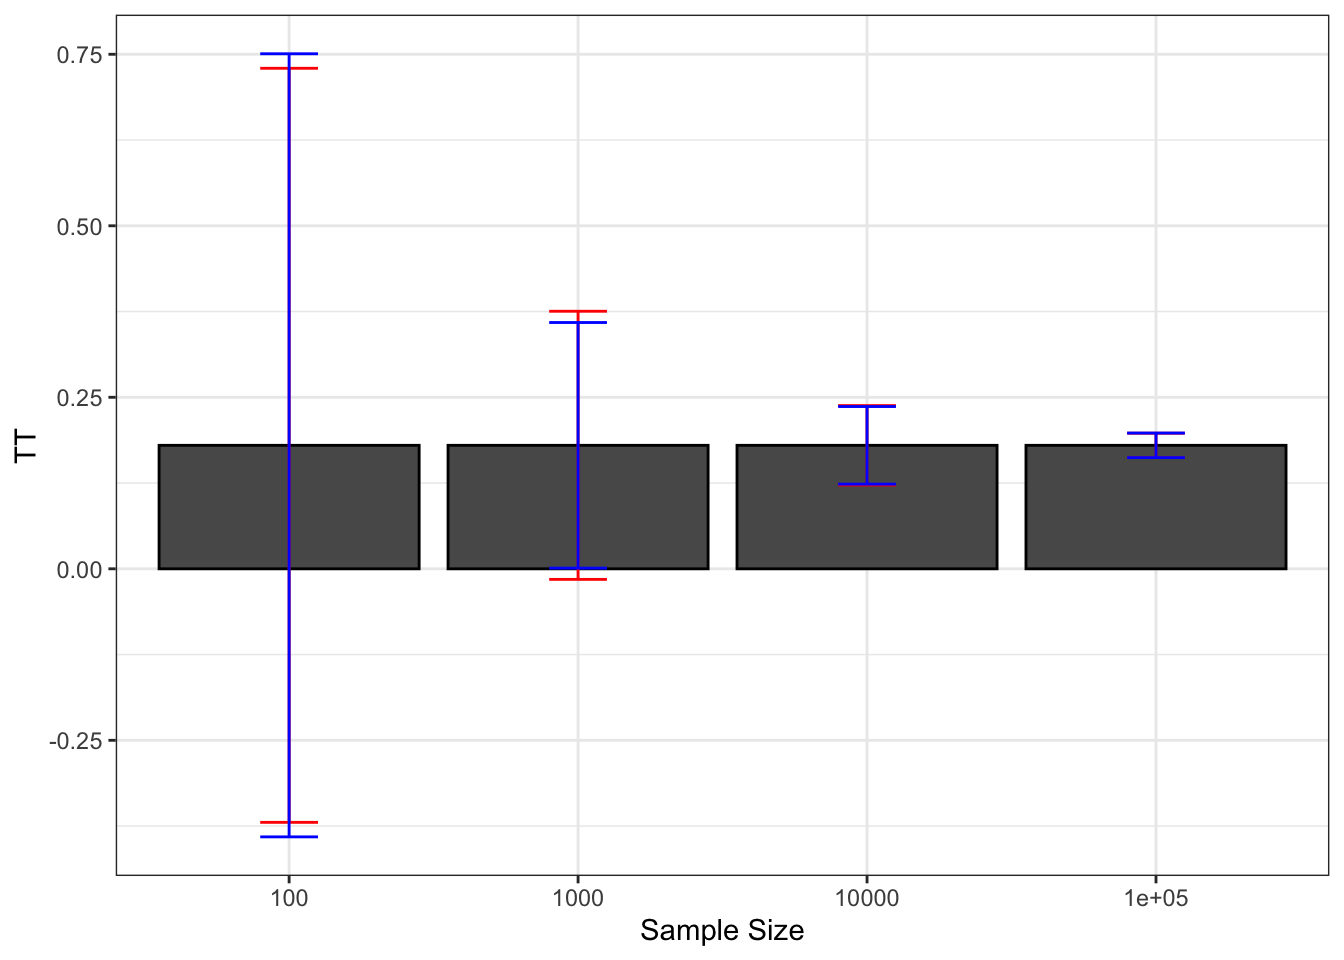
\includegraphics[width=0.6\linewidth]{STCI_files/figure-latex/sampnoisewwCLTplot-1} 

}

\caption{Average CLT-based approximations of sampling noise over replications of samples of different sizes (true sampling noise in red)}\label{fig:sampnoisewwCLTplot}
\end{figure}

\begin{Shaded}
\begin{Highlighting}[]
\NormalTok{N.plot <-}\StringTok{ }\DecValTok{40}
\NormalTok{plot.list <-}\StringTok{ }\KeywordTok{list}\NormalTok{()}

\ControlFlowTok{for}\NormalTok{ (k }\ControlFlowTok{in} \DecValTok{1}\OperatorTok{:}\KeywordTok{length}\NormalTok{(N.sample))\{}
  \KeywordTok{set.seed}\NormalTok{(}\DecValTok{1234}\NormalTok{)}
\NormalTok{  test.CLT <-}\StringTok{ }\NormalTok{simuls.ww[[k]][}\KeywordTok{sample}\NormalTok{(N.plot),}\KeywordTok{c}\NormalTok{(}\StringTok{'WW'}\NormalTok{,}\StringTok{'CLT.noise'}\NormalTok{)]}
\NormalTok{  test.CLT <-}\StringTok{ }\KeywordTok{as.data.frame}\NormalTok{(}\KeywordTok{cbind}\NormalTok{(test.CLT,}\KeywordTok{rep}\NormalTok{(}\KeywordTok{samp.noise}\NormalTok{(simuls.ww[[k]][,}\StringTok{'WW'}\NormalTok{],}\DataTypeTok{delta=}\NormalTok{delta),N.plot)))}
  \KeywordTok{colnames}\NormalTok{(test.CLT) <-}\StringTok{ }\KeywordTok{c}\NormalTok{(}\StringTok{'WW'}\NormalTok{,}\StringTok{'CLT.noise'}\NormalTok{,}\StringTok{'sampling.noise'}\NormalTok{)}
\NormalTok{  test.CLT}\OperatorTok{$}\NormalTok{id <-}\StringTok{ }\DecValTok{1}\OperatorTok{:}\NormalTok{N.plot}
\NormalTok{  plot.test.CLT <-}\StringTok{ }\KeywordTok{ggplot}\NormalTok{(test.CLT, }\KeywordTok{aes}\NormalTok{(}\DataTypeTok{x=}\KeywordTok{as.factor}\NormalTok{(id), }\DataTypeTok{y=}\NormalTok{WW)) }\OperatorTok{+}
\StringTok{      }\KeywordTok{geom_bar}\NormalTok{(}\DataTypeTok{position=}\KeywordTok{position_dodge}\NormalTok{(), }\DataTypeTok{stat=}\StringTok{"identity"}\NormalTok{, }\DataTypeTok{colour=}\StringTok{'black'}\NormalTok{) }\OperatorTok{+}
\StringTok{      }\KeywordTok{geom_errorbar}\NormalTok{(}\KeywordTok{aes}\NormalTok{(}\DataTypeTok{ymin=}\NormalTok{WW}\OperatorTok{-}\NormalTok{sampling.noise}\OperatorTok{/}\DecValTok{2}\NormalTok{, }\DataTypeTok{ymax=}\NormalTok{WW}\OperatorTok{+}\NormalTok{sampling.noise}\OperatorTok{/}\DecValTok{2}\NormalTok{), }\DataTypeTok{width=}\NormalTok{.}\DecValTok{2}\NormalTok{,}\DataTypeTok{position=}\KeywordTok{position_dodge}\NormalTok{(.}\DecValTok{9}\NormalTok{),}\DataTypeTok{color=}\StringTok{'red'}\NormalTok{) }\OperatorTok{+}
\StringTok{      }\KeywordTok{geom_errorbar}\NormalTok{(}\KeywordTok{aes}\NormalTok{(}\DataTypeTok{ymin=}\NormalTok{WW}\OperatorTok{-}\NormalTok{CLT.noise}\OperatorTok{/}\DecValTok{2}\NormalTok{, }\DataTypeTok{ymax=}\NormalTok{WW}\OperatorTok{+}\NormalTok{CLT.noise}\OperatorTok{/}\DecValTok{2}\NormalTok{), }\DataTypeTok{width=}\NormalTok{.}\DecValTok{2}\NormalTok{,}\DataTypeTok{position=}\KeywordTok{position_dodge}\NormalTok{(.}\DecValTok{9}\NormalTok{),}\DataTypeTok{color=}\StringTok{'blue'}\NormalTok{) }\OperatorTok{+}
\StringTok{      }\KeywordTok{geom_hline}\NormalTok{(}\KeywordTok{aes}\NormalTok{(}\DataTypeTok{yintercept=}\KeywordTok{delta.y.ate}\NormalTok{(param)), }\DataTypeTok{colour=}\StringTok{"#990000"}\NormalTok{, }\DataTypeTok{linetype=}\StringTok{"dashed"}\NormalTok{)}\OperatorTok{+}
\StringTok{      }\KeywordTok{xlab}\NormalTok{(}\StringTok{"Sample id"}\NormalTok{)}\OperatorTok{+}
\StringTok{      }\KeywordTok{theme_bw}\NormalTok{()}\OperatorTok{+}
\StringTok{      }\KeywordTok{ggtitle}\NormalTok{(}\KeywordTok{paste}\NormalTok{(}\StringTok{"N="}\NormalTok{,N.sample[k]))}
\NormalTok{  plot.list[[k]] <-}\StringTok{ }\NormalTok{plot.test.CLT}
\NormalTok{\}}
\NormalTok{plot.CI <-}\StringTok{ }\KeywordTok{plot_grid}\NormalTok{(plot.list[[}\DecValTok{1}\NormalTok{]],plot.list[[}\DecValTok{2}\NormalTok{]],plot.list[[}\DecValTok{3}\NormalTok{]],plot.list[[}\DecValTok{4}\NormalTok{]],}\DataTypeTok{ncol=}\DecValTok{1}\NormalTok{,}\DataTypeTok{nrow=}\KeywordTok{length}\NormalTok{(N.sample))}
\KeywordTok{print}\NormalTok{(plot.CI)}
\end{Highlighting}
\end{Shaded}

\begin{figure}[htbp]

{\centering 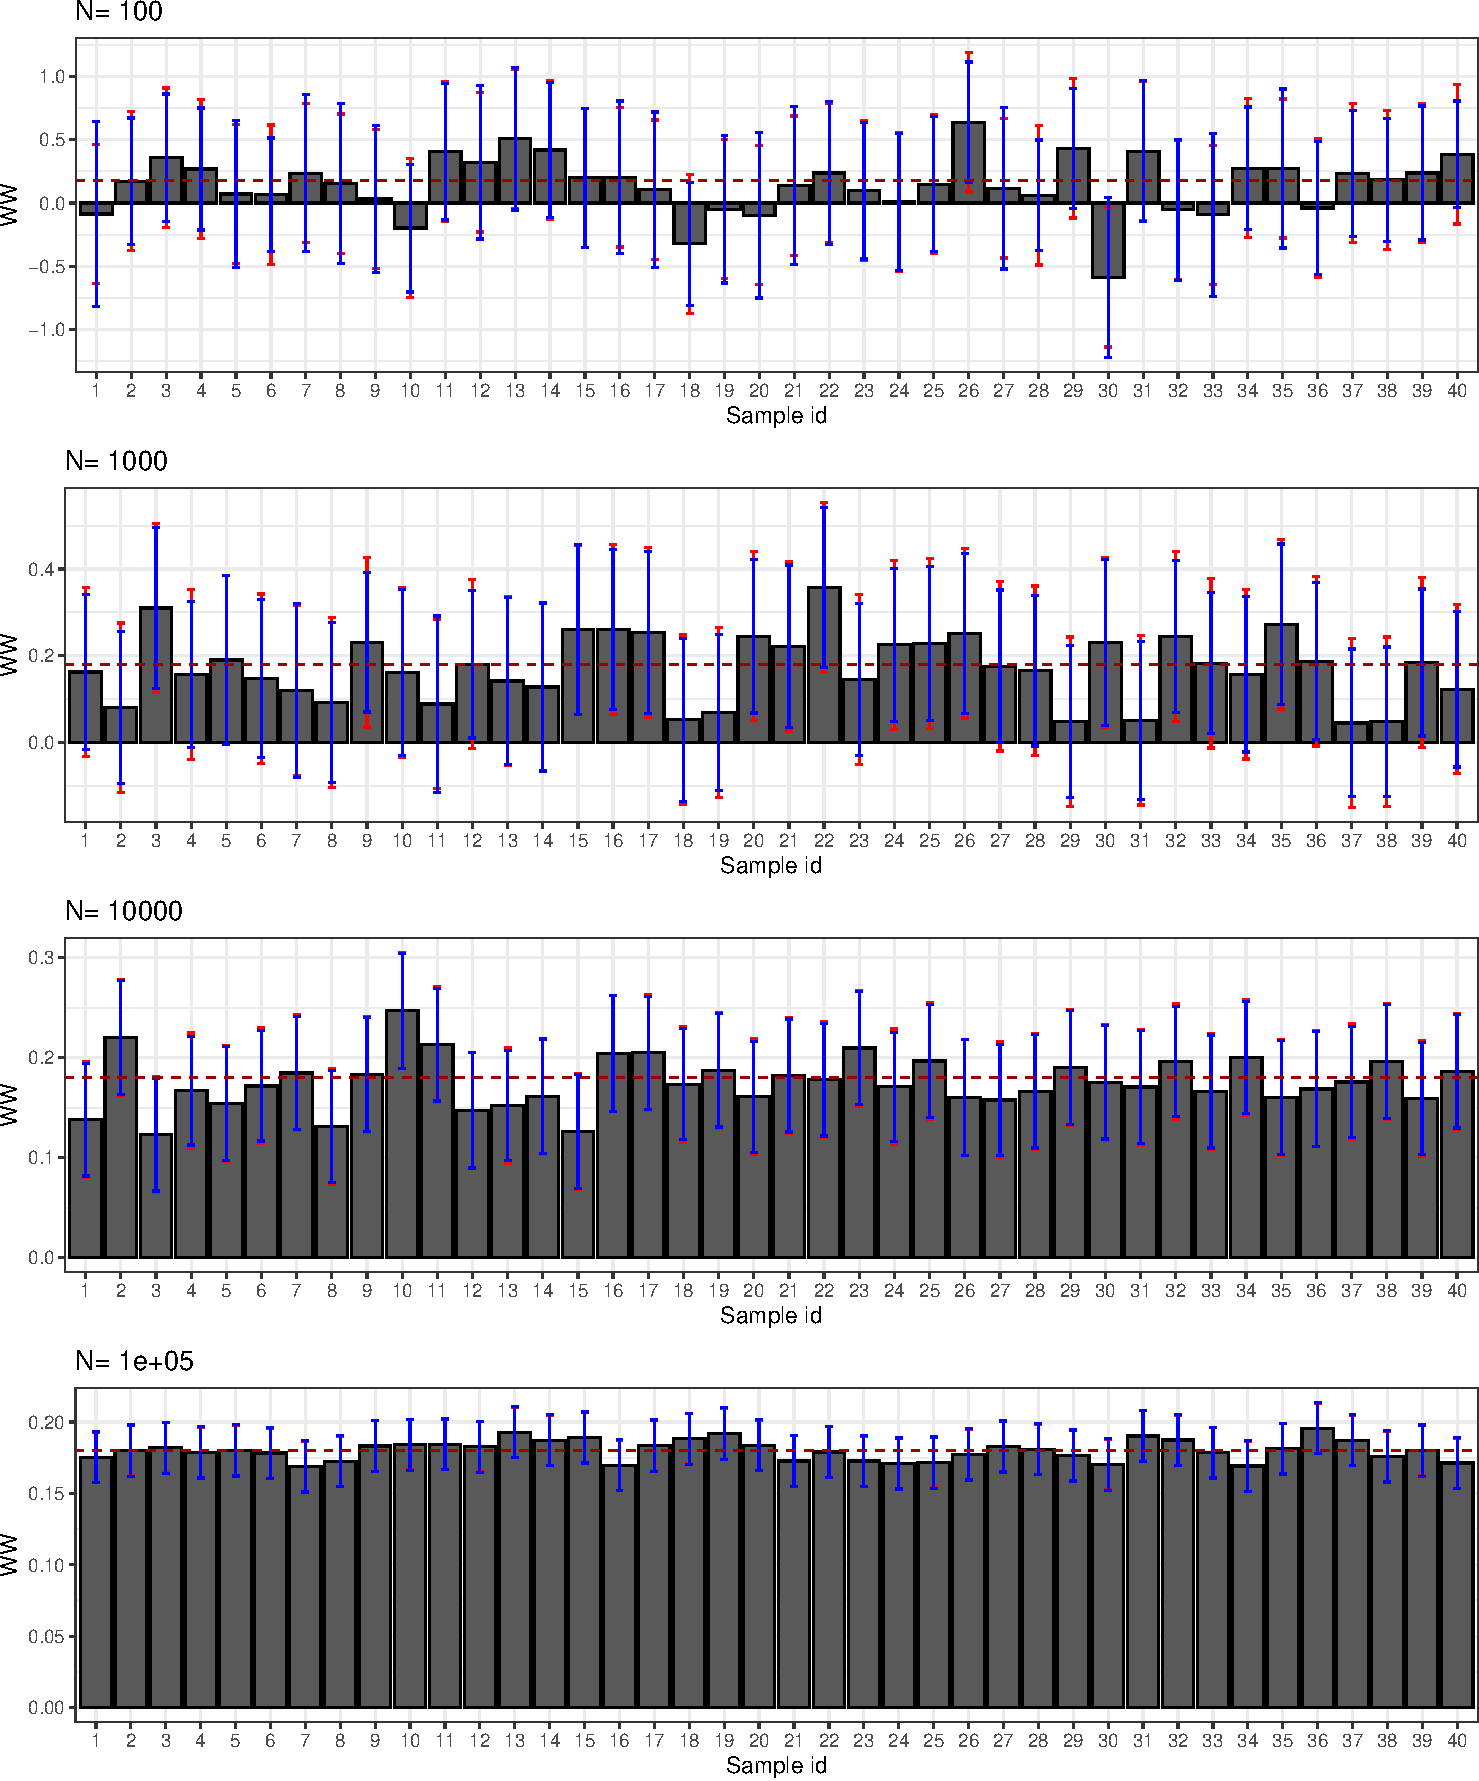
\includegraphics[width=0.6\linewidth]{STCI_files/figure-latex/confintervalCLT-1} 

}

\caption{CLT-based confidence intervals of $\hat{WW}$ for $\delta=$ 0.99 over sample replications for various sample sizes (true confidence intervals in red)}\label{fig:confintervalCLT}
\end{figure}

\BeginKnitrBlock{remark}
\iffalse{} {Remark. } \fi{}In proving the main result on the asymptotic
distribution of \(\hat{WW}\), we have also proved a very useful result:
\(\hat{WW}\) is the Ordinary Least Squares (OLS) estimator of \(\beta\)
in the regression \(Y_i=\alpha+\beta D_i + U_i\). This is pretty cool
since we now can use our classical OLS estimator in our statistical
package to estimate \(\hat{WW}\). Let's compute the OLS estimate of
\(WW\) in our sample:
\EndKnitrBlock{remark}

\begin{Shaded}
\begin{Highlighting}[]
\NormalTok{ols.ww <-}\StringTok{ }\KeywordTok{lm}\NormalTok{(y}\OperatorTok{~}\NormalTok{Ds)}
\NormalTok{ww.ols <-}\StringTok{ }\NormalTok{ols.ww}\OperatorTok{$}\NormalTok{coef[[}\DecValTok{2}\NormalTok{]]}
\end{Highlighting}
\end{Shaded}

We have \(\hat{WW}_{OLS}=\) 0.13 \(=\) 0.13 \(=\hat{WW}\).

\BeginKnitrBlock{remark}
\iffalse{} {Remark. } \fi{}Another pretty cool consequence of Theorem
\ref{thm:asympnoiseWW} and of its proof is that the standard error of
the OLS estimator of \(\hat{WW}\) (\(\sigma_{\beta}\)) is related to the
sampling noise of \(\hat{WW}\) by the following formula:
\(2\tilde{\epsilon}=2\Phi^{-1}\left(\frac{\delta+1}{2}\right)\sigma_{\beta}\).
\EndKnitrBlock{remark} This implies that sampling noise is equal to 5
\(\sigma_{\beta}\) when \(\delta=\) 0.99 and to 4 \(\sigma_{\beta}\)
when \(\delta=\) 0.95. It is thus very easy to move from estimates of
the standard error of the \(\beta\) coefficient to the extent of
sampling noise.

\BeginKnitrBlock{remark}
\iffalse{} {Remark. } \fi{}A last important consequence of Theorem
\ref{thm:asympnoiseWW} and of its proof is that the standard error of
the OLS estimator of \(\hat{WW}\) (\(\sigma_{\beta}\)) that we use is
the heteroskedasticity-robust one.
\EndKnitrBlock{remark} Using the RCM, we can indeed show that:

\begin{align*}
    \alpha & = \esp{Y_i^0|D_i=0}  \\
    \beta  & =  \Delta^Y_{TT} \\
    U_i    & = Y^0_i-\esp{Y^0_i|D_i=0} + D_i(\Delta^Y_i-\Delta^Y_{TT}),
    \end{align*}

Under Assumption \ref{def:noselb}, we have:

\begin{align*}
    U_i    & = (1-D_i)(Y^0_i-\esp{Y^0_i|D_i=0}) + D_i(Y_i^1-\esp{Y^1_i|D_i=1})
  \end{align*}

There is heteroskedasticity because the outcomes of the treated and of
the untreated have different variances:

\begin{align*}
    \var{U_i|D_i=d} & = \esp{U_i^2|D_i=d}  \\
                    & = \esp{(Y^d_i-\esp{Y^d_i|D_i=d})^2|D_i=d}  \\
                    & = \var{Y_i^d|D_i=d}
  \end{align*}

We do not want to assume homoskedasticity, since it would imply a
constant treatment effect. Indeed,
\(\var{Y_i^1|D_i=1} = \var{Y_i^0|D_i=1}+\var{\alpha_i|D_i=1}\).

\BeginKnitrBlock{remark}
\iffalse{} {Remark. } \fi{}In order to estimate the heteroskedasticity
robust standard error from the OLS regression, we can use the sandwich
package in R Most available heteroskedasticity robust estimators based
on the CLT can be written in the following way:
\EndKnitrBlock{remark}

\begin{align*}
  \var{\hat{\Theta}_{OLS}} & \approx (X'X)^{-1}X'\hat{\Omega}X(X'X)^{-1},
\end{align*}

where \(X\) is the matrix of regressors and
\(\hat{\Omega}=\diag(\hat{\sigma}^2_{U_1},\dots,\hat{\sigma}^2_{U_N})\)
is an estimate the covariance matrix of the residuals \(U_i\). Here are
various classical estimators for \(\hat{\Omega}\):

\begin{align*}
  \text{HC0:} & & \hat{\sigma_{U_i}}^2 & = \hat{U_i}^2 \\
  \text{HC1:} & & \hat{\sigma_{U_i}}^2 & = \frac{N}{N-K}\hat{U_i}^2 \\
  \text{HC2:} & & \hat{\sigma_{U_i}}^2 & = \frac{\hat{U_i}^2}{1-h_i} \\
  \text{HC3:} & & \hat{\sigma_{U_i}}^2 & = \frac{\hat{U_i}^2}{(1-h_i)^2}, 
\end{align*}

where \(\hat{U}_i\) is the residual from the OLS regression, \(K\) is
the number of regressors, \(h_i\) is the leverage of observation \(i\),
and is the \(i^{\text{th}}\) diagonal element of \(H=X(X'X)^{-1}X'\).
HC1 is the one reported by Stata when using the `robust' option.

\BeginKnitrBlock{example}
\protect\hypertarget{exm:unnamed-chunk-54}{}{\label{exm:unnamed-chunk-54}
}Using the sandwich package, we can estimate the
heteroskedasticity-robust variance-covariance matrix and sampling noise
as follows:
\EndKnitrBlock{example}

\begin{Shaded}
\begin{Highlighting}[]
\NormalTok{ols.ww.vcov.HC0 <-}\StringTok{ }\KeywordTok{vcovHC}\NormalTok{(ols.ww, }\DataTypeTok{type =} \StringTok{"HC0"}\NormalTok{)}
\NormalTok{samp.noise.ww.CLT.ols <-}\StringTok{ }\ControlFlowTok{function}\NormalTok{(delta,reg,...)\{}
  \KeywordTok{return}\NormalTok{(}\DecValTok{2}\OperatorTok{*}\KeywordTok{qnorm}\NormalTok{((delta}\OperatorTok{+}\DecValTok{1}\NormalTok{)}\OperatorTok{/}\DecValTok{2}\NormalTok{)}\OperatorTok{*}\KeywordTok{sqrt}\NormalTok{(}\KeywordTok{vcovHC}\NormalTok{(reg,...)[}\DecValTok{2}\NormalTok{,}\DecValTok{2}\NormalTok{]))}
\NormalTok{\}}
\end{Highlighting}
\end{Shaded}

For \(\delta=\) 0.99, sampling noise estimated using the ``HC0'' option
is equal to 0.35. This is exactly the value we have estimated using our
CLT-based formula (\(\hat{2\tilde{\epsilon}}=\) 0.35). Remember that
sampling noise is actually equal to 0.39. Other ``HC'' options might be
better in small samples. For example, with the ``HC1'' option, we have
an estimate for sampling noise of 0.35. What would have happened to our
estimate of sampling noise if we had ignored heteroskedasticity? The
default OLS standard error estimate yields an estimate for sampling
noise of 0.36.

\subsection{Using resampling methods}\label{sec:resamp}

The main intuition behind resampling methods is to use the sample as a
population, to draw samples from it and compute our estimator on each of
these samples in order to gauge its variability over sampling
repetitions. There are three main methods of resampling that work that
way: bootstrapping, radomization inference and subsampling.
Bootstrapping draws samples with replacement, so that each sample has
the same size as the original sample. Subsampling draws samples without
replacement, thereby the samples are of a smaller size than the original
one. Randomization inference keeps the same sample in all repetitions,
but changes the allocation of the treatment.

Why would we use resampling methods instead of CLT-based standard
errors? There are several possible reasons:

\begin{enumerate}
\def\labelenumi{\arabic{enumi}.}
\tightlist
\item
  Asymptotic refinements: sometimes, resampling methods are more precise
  in small samples than the CLT-based asymptotic approaches. In that
  case, we say that resampling methods offer asymptotic refinements.
\item
  Ease of computation: for some estimators, the CLT-based estimates of
  sampling noise are complex or cumbersome to compute, whereas
  resampling methods are only computationally intensive.
\item
  Inexistence of CLT-based estimates of sampling noise: some estimators
  do not have any CLT-based estimates of sampling noise yet. That was
  the case for the Nearest-Neighbour Matching estimator (NNM) for a long
  time for example. It still is the case for the Synthetic Control
  Method estimator. Beware though that the bootstrap is not valid for
  all estimators. For example, it is possible to show that the bootstrap
  is invalid for NNM. Subsampling is valid for NNM though (see Abadie
  and Imbens, 2006).
\end{enumerate}

\subsubsection{Bootstrap}\label{bootstrap}

The basic idea of the bootstrap is to use Monte Carlo replications to
draw samples from the original sample with replacement. Then, at each
replication, we compute the value of our estimator \(\hat{E}\) on the
new sample. Let's call this new value \(\hat{E}^*_k\) for bootstrap
replication \(k\). Under certain conditions, the distribution of
\(\hat{E}^*_k\) approximates the distribution of \(\hat{E}\) over sample
repetitions very well, and all the more so as the sample size gets
large.

What are the conditions under which the bootstrap is going to provide an
accurate estimation of the distribution of \(\hat{E}\)? Horowitz (2001)
reports on a very nice result by Mammen that makes these conditions
clear:

\BeginKnitrBlock{theorem}[Mammen (1992)]
\protect\hypertarget{thm:mammen92}{}{\label{thm:mammen92} \iffalse (Mammen
(1992)) \fi{} }Let \(\left\{X_i:i=1,\dots,N\right\}\) be a random sample
from a population. For a sequence of functions \(g_N\) and sequences of
numbers \(t_N\) and \(\sigma_N\), define
\(\bar{g}_N=\frac{1}{N}\sum_{i=1}^Ng_N(X_i)\) and
\(T_N=(\bar{g}_N-t_N)/\sigma_N\). For the bootstrap sample
\(\left\{X^*_i:i=1,\dots,N\right\}\), define
\(\bar{g}^*_N=\frac{1}{N}\sum_{i=1}^Ng_N(X^*_i)\) and
\(T^*_N=(\bar{g}^*_N-\bar{g}_N)/\sigma_N\). Let
\(G_N(\tau)=\Pr(T_N\leq\tau)\) and \(G^*_N(\tau)=\Pr(T^*_N\leq\tau)\),
where this last probability distribution is taken over bootstrap
sampling replications. Then \(G^*_N\) consistently estimates \(G_N\) if
and only if \(T_N\stackrel{d}{\rightarrow}\mathcal{N}(0,1)\).
\EndKnitrBlock{theorem}

Theorem \ref{thm:mammen92} states that the bootstrap will offer a
consistent estimation of the distribution of a given estimator if and
only if this estimator is asymptotically normally distributed. It means
that we could theoretically use the CLT-based asymptotic distribution to
compute sampling noise. So, and it demands to be stronlgy emphasized,
\textbf{the bootstrap is not valid when the CLT fails}.

How do we estimate sampling noise with the bootstrap? There are several
ways to do so, but I am going to emphasize the most widespread here,
that is known as the percentile method. Let's define
\(E^*_{\frac{1-\delta}{2}}\) and \(E^*_{\frac{1+\delta}{2}}\) as the
corresponding quantiles of the bootstrap distribution of \(\hat{E}^*_k\)
over a large number \(K\) of replications. The bootstrapped sampling
noise using the percentile method is simply the distance between these
two quantities.

\BeginKnitrBlock{theorem}[Bootstrapped Estimate of Sampling Noise of WW]
\protect\hypertarget{thm:bootnoiseWW}{}{\label{thm:bootnoiseWW}
\iffalse (Bootstrapped Estimate of Sampling Noise of WW) \fi{} }Under
Assumptions \ref{def:noselb}, \ref{def:fullrank}, \ref{def:iid} and
\ref{def:finitevar}, for a given confidence level \(\delta\) and sample
size \(N\), the sampling noise of \(\hat{WW}\) can be approximated as
follows:

\begin{align*}
2\epsilon & \approx E^*_{\frac{1+\delta}{2}}-E^*_{\frac{1-\delta}{2}} \equiv 2\tilde{\epsilon}^b.
\end{align*}
\EndKnitrBlock{theorem}

\BeginKnitrBlock{proof}
\iffalse{} {Proof. } \fi{}The \(WW\) estimator can be written as a sum:

\begin{align*}
\hat{\Delta^Y_{WW}} & = \frac{1}{N}\sum_{i=1}^N\frac{\left(Y_i-\frac{1}{N}\sum_{i=1}^NY_i\right)\left(D_i-\frac{1}{N}\sum_{i=1}^ND_i\right)}{\frac{1}{N}\sum_{i=1}^N\left(D_i-\frac{1}{N}\sum_{i=1}^ND_i\right)^2}.
\end{align*}

Using Lemma \ref{lem:asymWW}, we know that the \(WW\) estimator is
asymptotically normal under Assumptions \ref{def:noselb},
\ref{def:fullrank}, \ref{def:iid} and \ref{def:finitevar}. Using Theorem
\ref{thm:mammen92} proves the result.
\EndKnitrBlock{proof}

\BeginKnitrBlock{remark}
\iffalse{} {Remark. } \fi{}With the bootstrap, we are not going to
define the confidence interval using Theorem \ref{thm:confinter} but
directly using
\(\left\{E^*_{\frac{1-\delta}{2}};E^*_{\frac{1+\delta}{2}}\right\}\).
Indeed, we have defined the bootstrapped estimator of sampling noise by
using the asymetric confidence interval. We could have used the
equivalent of Definition \ref{def:sampnoise} on the bootstrapped samples
to compute sampling noise using the symmetric confidence interval. Both
are feasible and similar in large samples, since the asymptotic
distribution is symmetric. One advantage of asymetric confidence
intervals is that they might capture deviations from the normal
distribution in small samples. These advantages are part of what we call
asymptotic refinements. Rigorously, though, asymptotic refinements have
not been proved to exist for the percentile method but only for the
method bootstrapping asymptotically pivotal quantities.
\EndKnitrBlock{remark}

\BeginKnitrBlock{remark}
\iffalse{} {Remark. } \fi{}We say that a method brings asymptotic
refinements if it increases the precision when estimating sampling noise
and confidence intervals relative to the asymptotic CLT-based
approximation. The bootstrap has been shown rigorously to bring
asymptotic refinements when used to estimate the distribution of
asymptotically pivotal statistic. An asymptotically pivotal statistic is
a statistic that can be computed from the sample but that,
asymptotically, converges to a quantity that does not depend on the
sample, like for example a standard normal. Using Lemma
\ref{lem:asymWW}, we know for example that the following statistic is
asymptotically normal:
\EndKnitrBlock{remark}

\begin{align*}
  T_N^{WW} & = \frac{\hat{\Delta^Y_{WW}}-\Delta^Y_{TT}}{\sqrt{\frac{\frac{\var{Y_i^1|D_i=1}}{\Pr(D_i=1)}+\frac{\var{Y_i^0|D_i=0}}{1-\Pr(D_i=1)}}{N}}} \stackrel{d}{\rightarrow}\mathcal{N}\left(0,1\right).
\end{align*}

To build a confidence interval bootstrapping \(T_N^{WW}\), compute an
estimator of \(T_N^{WW}\) for each bootstrapped sample, say
\(\hat{T}_{N,k}^{WW*}\). You can for example use the OLS estimator in
the bootstrapped sample, with a heteroskedasticity-robust standard error
estimator. Or you can compute the \(WW\) estimator by hand in the sample
along with an estimator of its variance using the variance of the
outcomes in the treated and control groups. You can then estimate the
confidence interval as follows:
\(\left\{\hat{\Delta^Y_{WW}}-\hat{\sigma_{WW}}\hat{T}^{WW*}_{N,\frac{1-\delta}{2}};\hat{\Delta^Y_{WW}}+\hat{\sigma_{WW}}\hat{T}^{WW*}_{N,\frac{1+\delta}{2}}\right\}\),
where \(\hat{T}^{WW*}_{N,q}\) iq the \(q^{\text{th}}\) quantile of the
distribution of \(\hat{T}_{N,k}^{WW*}\) over sampling replications and
\(\hat{\sigma_{WW}}\) is an estimate of the variance of
\(\hat{\Delta^Y_{WW}}\) (either the CLT-based approximation of the
bootstrapped one, see below).

\BeginKnitrBlock{remark}
\iffalse{} {Remark. } \fi{}One last possibility to develop an estimator
for sampling noise and confidence interval is to use the bootstrap in
order to estimate the variance of the estimator \(\hat{E}\),
\(\hat{\sigma^2_{E}}\), and then use it to compute sampling noise. If
\(\hat{E}\) is asymptotically normally distributed, we have that
sampling noise is equal to
\(2\Phi^{-1}\left(\frac{\delta+1}{2}\right)\hat{\sigma_{E}}\). You can
use the usual formula from Theore \ref{thm:confinter} to compute the
confidence interval. The bootstrapped variance of \(\hat{E}\),
\(\hat{\sigma^2_{E}}\), is simply the variance of \(\hat{E}^*_k\) over
bootstrap replications.
\EndKnitrBlock{remark}

\BeginKnitrBlock{example}
\protect\hypertarget{exm:unnamed-chunk-59}{}{\label{exm:unnamed-chunk-59}
}In the numerical example, I am going to derive the bootstrapped
confidence intervals and sampling noise for the percentile method. Let's
first put the dataset from our example in a nice data frame format so
that resampling is made easier. We then define a function taking a
number of bootstrapped replications and spitting out sampling noise and
confidence intervals.
\EndKnitrBlock{example}

\begin{Shaded}
\begin{Highlighting}[]
\NormalTok{data <-}\StringTok{ }\KeywordTok{as.data.frame}\NormalTok{(}\KeywordTok{cbind}\NormalTok{(y,Ds,yB))}
\NormalTok{boot.fun.ww.}\DecValTok{1}\NormalTok{ <-}\StringTok{ }\ControlFlowTok{function}\NormalTok{(seed,data)\{}
  \KeywordTok{set.seed}\NormalTok{(seed,}\DataTypeTok{kind=}\StringTok{"Wichmann-Hill"}\NormalTok{)}
\NormalTok{  data <-}\StringTok{ }\NormalTok{data[}\KeywordTok{sample}\NormalTok{(}\KeywordTok{nrow}\NormalTok{(data),}\DataTypeTok{replace =} \OtherTok{TRUE}\NormalTok{),]}
\NormalTok{  ols.ww <-}\StringTok{ }\KeywordTok{lm}\NormalTok{(y}\OperatorTok{~}\NormalTok{Ds,}\DataTypeTok{data=}\NormalTok{data)}
\NormalTok{  ww <-}\StringTok{ }\NormalTok{ols.ww}\OperatorTok{$}\NormalTok{coef[[}\DecValTok{2}\NormalTok{]]}
  \KeywordTok{return}\NormalTok{(ww)}
\NormalTok{\}}

\NormalTok{boot.fun.ww <-}\StringTok{ }\ControlFlowTok{function}\NormalTok{(Nboot,data)\{}
  \CommentTok{#sfInit(parallel=TRUE,cpus=8)}
\NormalTok{  boot <-}\StringTok{ }\KeywordTok{lapply}\NormalTok{(}\DecValTok{1}\OperatorTok{:}\NormalTok{Nboot,boot.fun.ww.}\DecValTok{1}\NormalTok{,}\DataTypeTok{data=}\NormalTok{data)}
  \CommentTok{#sfStop()}
  \KeywordTok{return}\NormalTok{(}\KeywordTok{unlist}\NormalTok{(boot))}
\NormalTok{\}}

\NormalTok{boot.CI.ww <-}\StringTok{ }\ControlFlowTok{function}\NormalTok{(boot,delta)\{}
  \KeywordTok{return}\NormalTok{(}\KeywordTok{c}\NormalTok{(}\KeywordTok{quantile}\NormalTok{(boot,}\DataTypeTok{prob=}\NormalTok{(}\DecValTok{1}\OperatorTok{-}\NormalTok{delta)}\OperatorTok{/}\DecValTok{2}\NormalTok{),}\KeywordTok{quantile}\NormalTok{(boot,}\DataTypeTok{prob=}\NormalTok{(}\DecValTok{1}\OperatorTok{+}\NormalTok{delta)}\OperatorTok{/}\DecValTok{2}\NormalTok{)))}
\NormalTok{\}}

\NormalTok{boot.samp.noise.ww <-}\StringTok{ }\ControlFlowTok{function}\NormalTok{(boot,delta)\{}
  \KeywordTok{return}\NormalTok{(}\KeywordTok{quantile}\NormalTok{(boot,}\DataTypeTok{prob=}\NormalTok{(}\DecValTok{1}\OperatorTok{+}\NormalTok{delta)}\OperatorTok{/}\DecValTok{2}\NormalTok{)}\OperatorTok{-}\KeywordTok{quantile}\NormalTok{(boot,}\DataTypeTok{prob=}\NormalTok{(}\DecValTok{1}\OperatorTok{-}\NormalTok{delta)}\OperatorTok{/}\DecValTok{2}\NormalTok{))}
\NormalTok{\}}

\NormalTok{Nboot <-}\StringTok{ }\DecValTok{500}
\NormalTok{ww.boot <-}\StringTok{ }\KeywordTok{boot.fun.ww}\NormalTok{(Nboot,data)}
\NormalTok{ww.CI.boot <-}\StringTok{ }\KeywordTok{boot.CI.ww}\NormalTok{(ww.boot,delta)}
\NormalTok{ww.samp.noise.boot <-}\StringTok{ }\KeywordTok{boot.samp.noise.ww}\NormalTok{(ww.boot,delta)}
\end{Highlighting}
\end{Shaded}

Over 500 replications, the 99\% bootstrapped confidence interval using
the percentile method is \(\left\{-0.023;0.316\right\}\). As a
consequence, the bootstrapped estimate of 99\% sampling noise is of
0.339. Remember that, with \(N=\) 1000, sampling noise is actually equal
to 0.39.

In order to assess the global precision of bootstrapping, we are going
to resort to Monte Carlo simulations. For each Monte Carlo sample, we
are going to estimate sampling noise and confidence intervals using the
bootstrap. As you can imagine, this is going to prove rather
computationally intensive. I cannot use parallelization twice: I have to
choose whether to parallelize the Monte Carlo simulations or the
bootstrap simulations. I have choosen to parallelize the outer loop, so
that a given job takes longer on each cluster.

\begin{Shaded}
\begin{Highlighting}[]
\NormalTok{monte.carlo.ww.boot <-}\StringTok{ }\ControlFlowTok{function}\NormalTok{(s,N,param,Nboot,delta)\{}
  \KeywordTok{set.seed}\NormalTok{(s)}
\NormalTok{  mu <-}\StringTok{ }\KeywordTok{rnorm}\NormalTok{(N,param[}\StringTok{"barmu"}\NormalTok{],}\KeywordTok{sqrt}\NormalTok{(param[}\StringTok{"sigma2mu"}\NormalTok{]))}
\NormalTok{  UB <-}\StringTok{ }\KeywordTok{rnorm}\NormalTok{(N,}\DecValTok{0}\NormalTok{,}\KeywordTok{sqrt}\NormalTok{(param[}\StringTok{"sigma2U"}\NormalTok{]))}
\NormalTok{  yB <-}\StringTok{ }\NormalTok{mu }\OperatorTok{+}\StringTok{ }\NormalTok{UB }
\NormalTok{  YB <-}\StringTok{ }\KeywordTok{exp}\NormalTok{(yB)}
\NormalTok{  Ds <-}\StringTok{ }\KeywordTok{rep}\NormalTok{(}\DecValTok{0}\NormalTok{,N)}
\NormalTok{  V <-}\StringTok{ }\KeywordTok{rnorm}\NormalTok{(N,param[}\StringTok{"barmu"}\NormalTok{],}\KeywordTok{sqrt}\NormalTok{(param[}\StringTok{"sigma2mu"}\NormalTok{]}\OperatorTok{+}\NormalTok{param[}\StringTok{"sigma2U"}\NormalTok{]))}
\NormalTok{  Ds[V}\OperatorTok{<=}\KeywordTok{log}\NormalTok{(param[}\StringTok{"barY"}\NormalTok{])] <-}\StringTok{ }\DecValTok{1} 
\NormalTok{  epsilon <-}\StringTok{ }\KeywordTok{rnorm}\NormalTok{(N,}\DecValTok{0}\NormalTok{,}\KeywordTok{sqrt}\NormalTok{(param[}\StringTok{"sigma2epsilon"}\NormalTok{]))}
\NormalTok{  eta<-}\StringTok{ }\KeywordTok{rnorm}\NormalTok{(N,}\DecValTok{0}\NormalTok{,}\KeywordTok{sqrt}\NormalTok{(param[}\StringTok{"sigma2eta"}\NormalTok{]))}
\NormalTok{  U0 <-}\StringTok{ }\NormalTok{param[}\StringTok{"rho"}\NormalTok{]}\OperatorTok{*}\NormalTok{UB }\OperatorTok{+}\StringTok{ }\NormalTok{epsilon}
\NormalTok{  y0 <-}\StringTok{ }\NormalTok{mu }\OperatorTok{+}\StringTok{  }\NormalTok{U0 }\OperatorTok{+}\StringTok{ }\NormalTok{param[}\StringTok{"delta"}\NormalTok{]}
\NormalTok{  alpha <-}\StringTok{ }\NormalTok{param[}\StringTok{"baralpha"}\NormalTok{]}\OperatorTok{+}\StringTok{  }\NormalTok{param[}\StringTok{"theta"}\NormalTok{]}\OperatorTok{*}\NormalTok{mu }\OperatorTok{+}\StringTok{ }\NormalTok{eta}
\NormalTok{  y1 <-}\StringTok{ }\NormalTok{y0}\OperatorTok{+}\NormalTok{alpha}
\NormalTok{  Y0 <-}\StringTok{ }\KeywordTok{exp}\NormalTok{(y0)}
\NormalTok{  Y1 <-}\StringTok{ }\KeywordTok{exp}\NormalTok{(y1)}
\NormalTok{  y <-}\StringTok{ }\NormalTok{y1}\OperatorTok{*}\NormalTok{Ds}\OperatorTok{+}\NormalTok{y0}\OperatorTok{*}\NormalTok{(}\DecValTok{1}\OperatorTok{-}\NormalTok{Ds)}
\NormalTok{  Y <-}\StringTok{ }\NormalTok{Y1}\OperatorTok{*}\NormalTok{Ds}\OperatorTok{+}\NormalTok{Y0}\OperatorTok{*}\NormalTok{(}\DecValTok{1}\OperatorTok{-}\NormalTok{Ds)}
\NormalTok{  data <-}\StringTok{ }\KeywordTok{as.data.frame}\NormalTok{(}\KeywordTok{cbind}\NormalTok{(y,Ds,yB))}
\NormalTok{  ww.boot <-}\StringTok{ }\KeywordTok{boot.fun.ww}\NormalTok{(Nboot,data)}
\NormalTok{  ww.CI.boot <-}\StringTok{ }\KeywordTok{boot.CI.ww}\NormalTok{(ww.boot,delta)}
\NormalTok{  ww.samp.noise.boot <-}\StringTok{ }\KeywordTok{boot.samp.noise.ww}\NormalTok{(ww.boot,delta)}
  \KeywordTok{return}\NormalTok{(}\KeywordTok{c}\NormalTok{((}\DecValTok{1}\OperatorTok{/}\KeywordTok{sum}\NormalTok{(Ds))}\OperatorTok{*}\KeywordTok{sum}\NormalTok{(y}\OperatorTok{*}\NormalTok{Ds)}\OperatorTok{-}\NormalTok{(}\DecValTok{1}\OperatorTok{/}\KeywordTok{sum}\NormalTok{(}\DecValTok{1}\OperatorTok{-}\NormalTok{Ds))}\OperatorTok{*}\KeywordTok{sum}\NormalTok{(y}\OperatorTok{*}\NormalTok{(}\DecValTok{1}\OperatorTok{-}\NormalTok{Ds)),}\KeywordTok{var}\NormalTok{(y[Ds}\OperatorTok{==}\DecValTok{1}\NormalTok{]),}\KeywordTok{var}\NormalTok{(y[Ds}\OperatorTok{==}\DecValTok{0}\NormalTok{]),}\KeywordTok{mean}\NormalTok{(Ds),ww.CI.boot[[}\DecValTok{1}\NormalTok{]],ww.CI.boot[[}\DecValTok{2}\NormalTok{]],ww.samp.noise.boot))}
\NormalTok{\}}

\NormalTok{sf.simuls.ww.N.boot <-}\StringTok{ }\ControlFlowTok{function}\NormalTok{(N,Nsim,Nboot,delta,param)\{}
  \KeywordTok{sfInit}\NormalTok{(}\DataTypeTok{parallel=}\OtherTok{TRUE}\NormalTok{,}\DataTypeTok{cpus=}\DecValTok{2}\OperatorTok{*}\NormalTok{ncpus)}
  \KeywordTok{sfExport}\NormalTok{(}\StringTok{"boot.fun.ww"}\NormalTok{,}\StringTok{"boot.CI.ww"}\NormalTok{,}\StringTok{"boot.samp.noise.ww"}\NormalTok{,}\StringTok{"boot.fun.ww.1"}\NormalTok{)}
\NormalTok{  sim <-}\StringTok{ }\KeywordTok{as.data.frame}\NormalTok{(}\KeywordTok{matrix}\NormalTok{(}\KeywordTok{unlist}\NormalTok{(}\KeywordTok{sfLapply}\NormalTok{(}\DecValTok{1}\OperatorTok{:}\NormalTok{Nsim,monte.carlo.ww.boot,}\DataTypeTok{N=}\NormalTok{N,}\DataTypeTok{Nboot=}\NormalTok{Nboot,}\DataTypeTok{delta=}\NormalTok{delta,}\DataTypeTok{param=}\NormalTok{param)),}\DataTypeTok{nrow=}\NormalTok{Nsim,}\DataTypeTok{ncol=}\DecValTok{7}\NormalTok{,}\DataTypeTok{byrow=}\OtherTok{TRUE}\NormalTok{))}
  \KeywordTok{sfStop}\NormalTok{()}
  \KeywordTok{colnames}\NormalTok{(sim) <-}\StringTok{ }\KeywordTok{c}\NormalTok{(}\StringTok{'WW'}\NormalTok{,}\StringTok{'V1'}\NormalTok{,}\StringTok{'V0'}\NormalTok{,}\StringTok{'p'}\NormalTok{,}\StringTok{'boot.lCI'}\NormalTok{,}\StringTok{'boot.uCI'}\NormalTok{,}\StringTok{'boot.samp.noise'}\NormalTok{)}
  \KeywordTok{return}\NormalTok{(sim)}
\NormalTok{\}}

\NormalTok{simuls.ww.boot <-}\StringTok{ }\KeywordTok{lapply}\NormalTok{(N.sample,sf.simuls.ww.N.boot,}\DataTypeTok{Nsim=}\NormalTok{Nsim,}\DataTypeTok{param=}\NormalTok{param,}\DataTypeTok{Nboot=}\NormalTok{Nboot,}\DataTypeTok{delta=}\NormalTok{delta)}
\end{Highlighting}
\end{Shaded}

We can now graph our bootstrapped estimate of sampling noise in all of
our samples, the average bootstrapped estimates of sampling noise and of
confidence intervals, in Figures \ref{fig:sampnoisewwbootall},
\ref{fig:sampnoisewwbootplot} and \ref{fig:confintervalboot} show.

\begin{Shaded}
\begin{Highlighting}[]
\KeywordTok{par}\NormalTok{(}\DataTypeTok{mfrow=}\KeywordTok{c}\NormalTok{(}\DecValTok{2}\NormalTok{,}\DecValTok{2}\NormalTok{))}
\ControlFlowTok{for}\NormalTok{ (i }\ControlFlowTok{in} \DecValTok{1}\OperatorTok{:}\DecValTok{4}\NormalTok{)\{}
  \KeywordTok{hist}\NormalTok{(simuls.ww.boot[[i]][,}\StringTok{'boot.samp.noise'}\NormalTok{],}\DataTypeTok{main=}\KeywordTok{paste}\NormalTok{(}\StringTok{'N='}\NormalTok{,}\KeywordTok{as.character}\NormalTok{(N.sample[i])),}\DataTypeTok{xlab=}\KeywordTok{expression}\NormalTok{(}\KeywordTok{hat}\NormalTok{(}\DecValTok{2}\OperatorTok{*}\KeywordTok{bar}\NormalTok{(epsilon))),}\DataTypeTok{xlim=}\KeywordTok{c}\NormalTok{(}\KeywordTok{min}\NormalTok{(simuls.ww.boot[[i]][,}\StringTok{'boot.samp.noise'}\NormalTok{]),}\KeywordTok{max}\NormalTok{(simuls.ww.boot[[i]][,}\StringTok{'boot.samp.noise'}\NormalTok{])))}
  \KeywordTok{abline}\NormalTok{(}\DataTypeTok{v=}\NormalTok{table.noise[i,}\KeywordTok{colnames}\NormalTok{(table.noise)}\OperatorTok{==}\StringTok{'sampling.noise'}\NormalTok{],}\DataTypeTok{col=}\StringTok{"red"}\NormalTok{)}
\NormalTok{\}}
\end{Highlighting}
\end{Shaded}

\begin{figure}[htbp]

{\centering 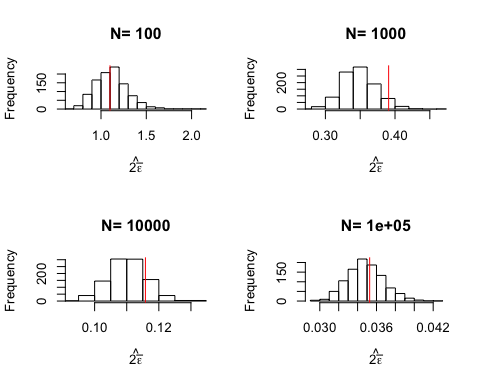
\includegraphics[width=0.6\linewidth]{STCI_files/figure-latex/sampnoisewwbootall-1} 

}

\caption{Distribution of the bootstrapped approximation of sampling noise over replications of samples of different sizes (true sampling noise in red)}\label{fig:sampnoisewwbootall}
\end{figure}

\begin{Shaded}
\begin{Highlighting}[]
\ControlFlowTok{for}\NormalTok{ (k }\ControlFlowTok{in}\NormalTok{ (}\DecValTok{1}\OperatorTok{:}\KeywordTok{length}\NormalTok{(N.sample)))\{}
\NormalTok{  table.noise}\OperatorTok{$}\NormalTok{boot.noise[k] <-}\StringTok{ }\KeywordTok{mean}\NormalTok{(simuls.ww.boot[[k]]}\OperatorTok{$}\NormalTok{boot.samp.noise)}
\NormalTok{\}}
\KeywordTok{ggplot}\NormalTok{(table.noise, }\KeywordTok{aes}\NormalTok{(}\DataTypeTok{x=}\KeywordTok{as.factor}\NormalTok{(N), }\DataTypeTok{y=}\NormalTok{TT)) }\OperatorTok{+}
\StringTok{  }\KeywordTok{geom_bar}\NormalTok{(}\DataTypeTok{position=}\KeywordTok{position_dodge}\NormalTok{(), }\DataTypeTok{stat=}\StringTok{"identity"}\NormalTok{, }\DataTypeTok{colour=}\StringTok{'black'}\NormalTok{) }\OperatorTok{+}
\StringTok{  }\KeywordTok{geom_errorbar}\NormalTok{(}\KeywordTok{aes}\NormalTok{(}\DataTypeTok{ymin=}\NormalTok{TT}\OperatorTok{-}\NormalTok{sampling.noise}\OperatorTok{/}\DecValTok{2}\NormalTok{, }\DataTypeTok{ymax=}\NormalTok{TT}\OperatorTok{+}\NormalTok{sampling.noise}\OperatorTok{/}\DecValTok{2}\NormalTok{), }\DataTypeTok{width=}\NormalTok{.}\DecValTok{2}\NormalTok{,}\DataTypeTok{position=}\KeywordTok{position_dodge}\NormalTok{(.}\DecValTok{9}\NormalTok{),}\DataTypeTok{color=}\StringTok{'red'}\NormalTok{) }\OperatorTok{+}
\StringTok{  }\KeywordTok{geom_errorbar}\NormalTok{(}\KeywordTok{aes}\NormalTok{(}\DataTypeTok{ymin=}\NormalTok{TT}\OperatorTok{-}\NormalTok{boot.noise}\OperatorTok{/}\DecValTok{2}\NormalTok{, }\DataTypeTok{ymax=}\NormalTok{TT}\OperatorTok{+}\NormalTok{boot.noise}\OperatorTok{/}\DecValTok{2}\NormalTok{), }\DataTypeTok{width=}\NormalTok{.}\DecValTok{2}\NormalTok{,}\DataTypeTok{position=}\KeywordTok{position_dodge}\NormalTok{(.}\DecValTok{9}\NormalTok{),}\DataTypeTok{color=}\StringTok{'blue'}\NormalTok{) }\OperatorTok{+}
\StringTok{  }\KeywordTok{xlab}\NormalTok{(}\StringTok{"Sample Size"}\NormalTok{)}\OperatorTok{+}
\StringTok{  }\KeywordTok{theme_bw}\NormalTok{()}
\end{Highlighting}
\end{Shaded}

\begin{figure}[htbp]

{\centering 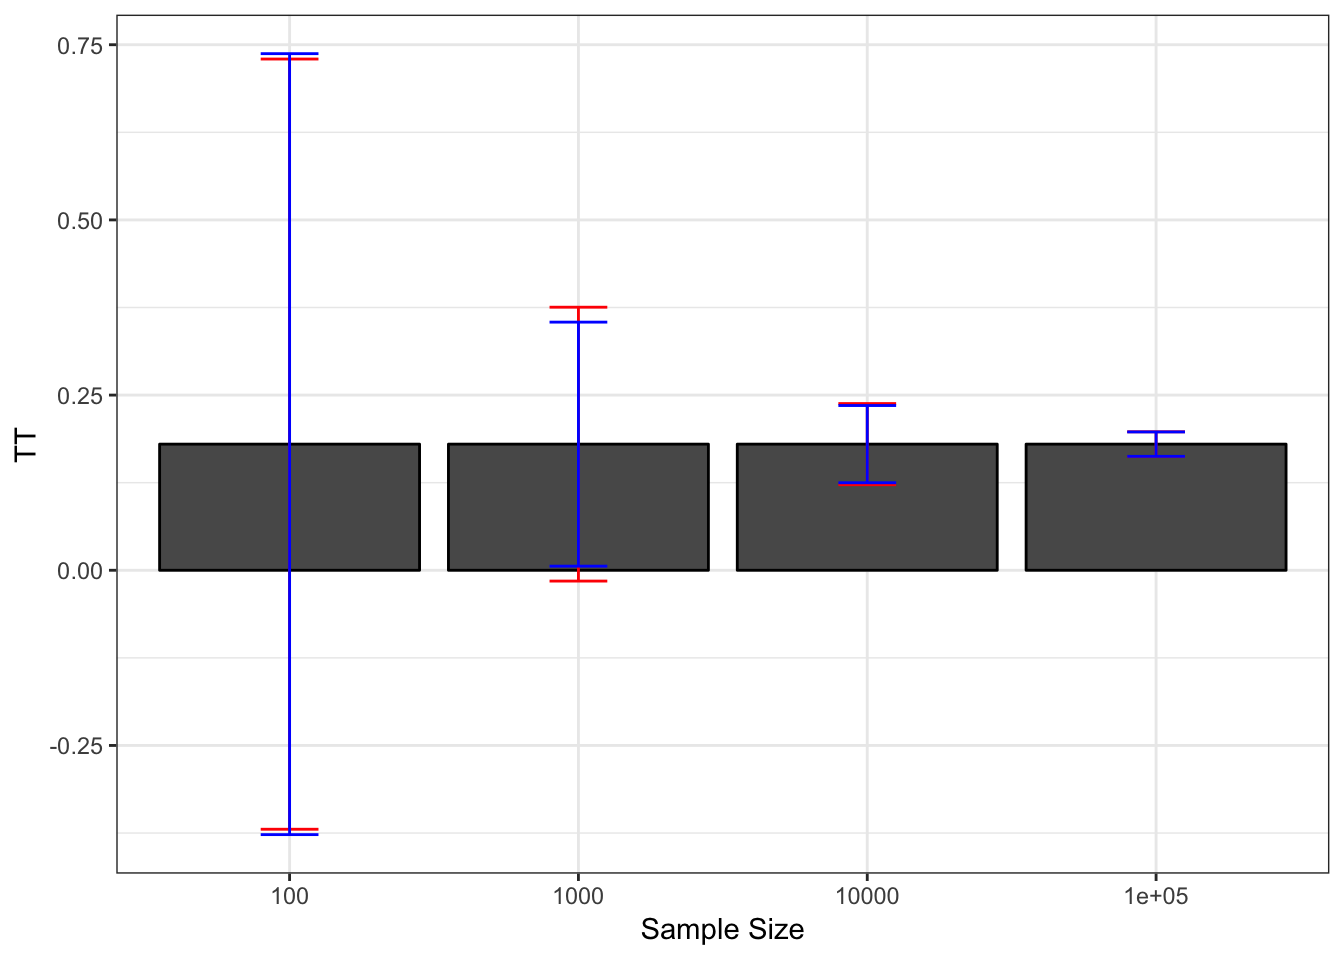
\includegraphics[width=0.6\linewidth]{STCI_files/figure-latex/sampnoisewwbootplot-1} 

}

\caption{Average bootstrapped approximations of sampling noise over replications of samples of different sizes (true sampling noise in red)}\label{fig:sampnoisewwbootplot}
\end{figure}

\begin{Shaded}
\begin{Highlighting}[]
\NormalTok{N.plot <-}\StringTok{ }\DecValTok{40}
\NormalTok{plot.list <-}\StringTok{ }\KeywordTok{list}\NormalTok{()}

\ControlFlowTok{for}\NormalTok{ (k }\ControlFlowTok{in} \DecValTok{1}\OperatorTok{:}\KeywordTok{length}\NormalTok{(N.sample))\{}
 \KeywordTok{set.seed}\NormalTok{(}\DecValTok{1234}\NormalTok{)}
\NormalTok{ test.boot <-}\StringTok{ }\NormalTok{simuls.ww.boot[[k]][}\KeywordTok{sample}\NormalTok{(N.plot),}\KeywordTok{c}\NormalTok{(}\StringTok{'WW'}\NormalTok{,}\StringTok{'boot.lCI'}\NormalTok{,}\StringTok{'boot.uCI'}\NormalTok{)]}
\NormalTok{ test.boot <-}\StringTok{ }\KeywordTok{as.data.frame}\NormalTok{(}\KeywordTok{cbind}\NormalTok{(test.boot,}\KeywordTok{rep}\NormalTok{(}\KeywordTok{samp.noise}\NormalTok{(simuls.ww.boot[[k]][,}\StringTok{'WW'}\NormalTok{],}\DataTypeTok{delta=}\NormalTok{delta),N.plot)))}
 \KeywordTok{colnames}\NormalTok{(test.boot) <-}\StringTok{ }\KeywordTok{c}\NormalTok{(}\StringTok{'WW'}\NormalTok{,}\StringTok{'boot.lCI'}\NormalTok{,}\StringTok{'boot.uCI'}\NormalTok{,}\StringTok{'sampling.noise'}\NormalTok{)}
\NormalTok{ test.boot}\OperatorTok{$}\NormalTok{id <-}\StringTok{ }\DecValTok{1}\OperatorTok{:}\NormalTok{N.plot}
\NormalTok{ plot.test.boot <-}\StringTok{ }\KeywordTok{ggplot}\NormalTok{(test.boot, }\KeywordTok{aes}\NormalTok{(}\DataTypeTok{x=}\KeywordTok{as.factor}\NormalTok{(id), }\DataTypeTok{y=}\NormalTok{WW)) }\OperatorTok{+}
\StringTok{     }\KeywordTok{geom_bar}\NormalTok{(}\DataTypeTok{position=}\KeywordTok{position_dodge}\NormalTok{(), }\DataTypeTok{stat=}\StringTok{"identity"}\NormalTok{, }\DataTypeTok{colour=}\StringTok{'black'}\NormalTok{) }\OperatorTok{+}
\StringTok{     }\KeywordTok{geom_errorbar}\NormalTok{(}\KeywordTok{aes}\NormalTok{(}\DataTypeTok{ymin=}\NormalTok{WW}\OperatorTok{-}\NormalTok{sampling.noise}\OperatorTok{/}\DecValTok{2}\NormalTok{, }\DataTypeTok{ymax=}\NormalTok{WW}\OperatorTok{+}\NormalTok{sampling.noise}\OperatorTok{/}\DecValTok{2}\NormalTok{), }\DataTypeTok{width=}\NormalTok{.}\DecValTok{2}\NormalTok{,}\DataTypeTok{position=}\KeywordTok{position_dodge}\NormalTok{(.}\DecValTok{9}\NormalTok{),}\DataTypeTok{color=}\StringTok{'red'}\NormalTok{) }\OperatorTok{+}
\StringTok{     }\KeywordTok{geom_errorbar}\NormalTok{(}\KeywordTok{aes}\NormalTok{(}\DataTypeTok{ymin=}\NormalTok{boot.lCI, }\DataTypeTok{ymax=}\NormalTok{boot.uCI), }\DataTypeTok{width=}\NormalTok{.}\DecValTok{2}\NormalTok{,}\DataTypeTok{position=}\KeywordTok{position_dodge}\NormalTok{(.}\DecValTok{9}\NormalTok{),}\DataTypeTok{color=}\StringTok{'blue'}\NormalTok{) }\OperatorTok{+}
\StringTok{     }\KeywordTok{geom_hline}\NormalTok{(}\KeywordTok{aes}\NormalTok{(}\DataTypeTok{yintercept=}\KeywordTok{delta.y.ate}\NormalTok{(param)), }\DataTypeTok{colour=}\StringTok{"#990000"}\NormalTok{, }\DataTypeTok{linetype=}\StringTok{"dashed"}\NormalTok{)}\OperatorTok{+}
\StringTok{     }\KeywordTok{xlab}\NormalTok{(}\StringTok{"Sample id"}\NormalTok{)}\OperatorTok{+}
\StringTok{     }\KeywordTok{theme_bw}\NormalTok{()}\OperatorTok{+}
\StringTok{     }\KeywordTok{ggtitle}\NormalTok{(}\KeywordTok{paste}\NormalTok{(}\StringTok{"N="}\NormalTok{,N.sample[k]))}
\NormalTok{ plot.list[[k]] <-}\StringTok{ }\NormalTok{plot.test.boot}
\NormalTok{\}}
\NormalTok{plot.CI <-}\StringTok{ }\KeywordTok{plot_grid}\NormalTok{(plot.list[[}\DecValTok{1}\NormalTok{]],plot.list[[}\DecValTok{2}\NormalTok{]],plot.list[[}\DecValTok{3}\NormalTok{]],plot.list[[}\DecValTok{4}\NormalTok{]],}\DataTypeTok{ncol=}\DecValTok{1}\NormalTok{,}\DataTypeTok{nrow=}\KeywordTok{length}\NormalTok{(N.sample))}
\KeywordTok{print}\NormalTok{(plot.CI)}
\end{Highlighting}
\end{Shaded}

\begin{figure}[htbp]

{\centering 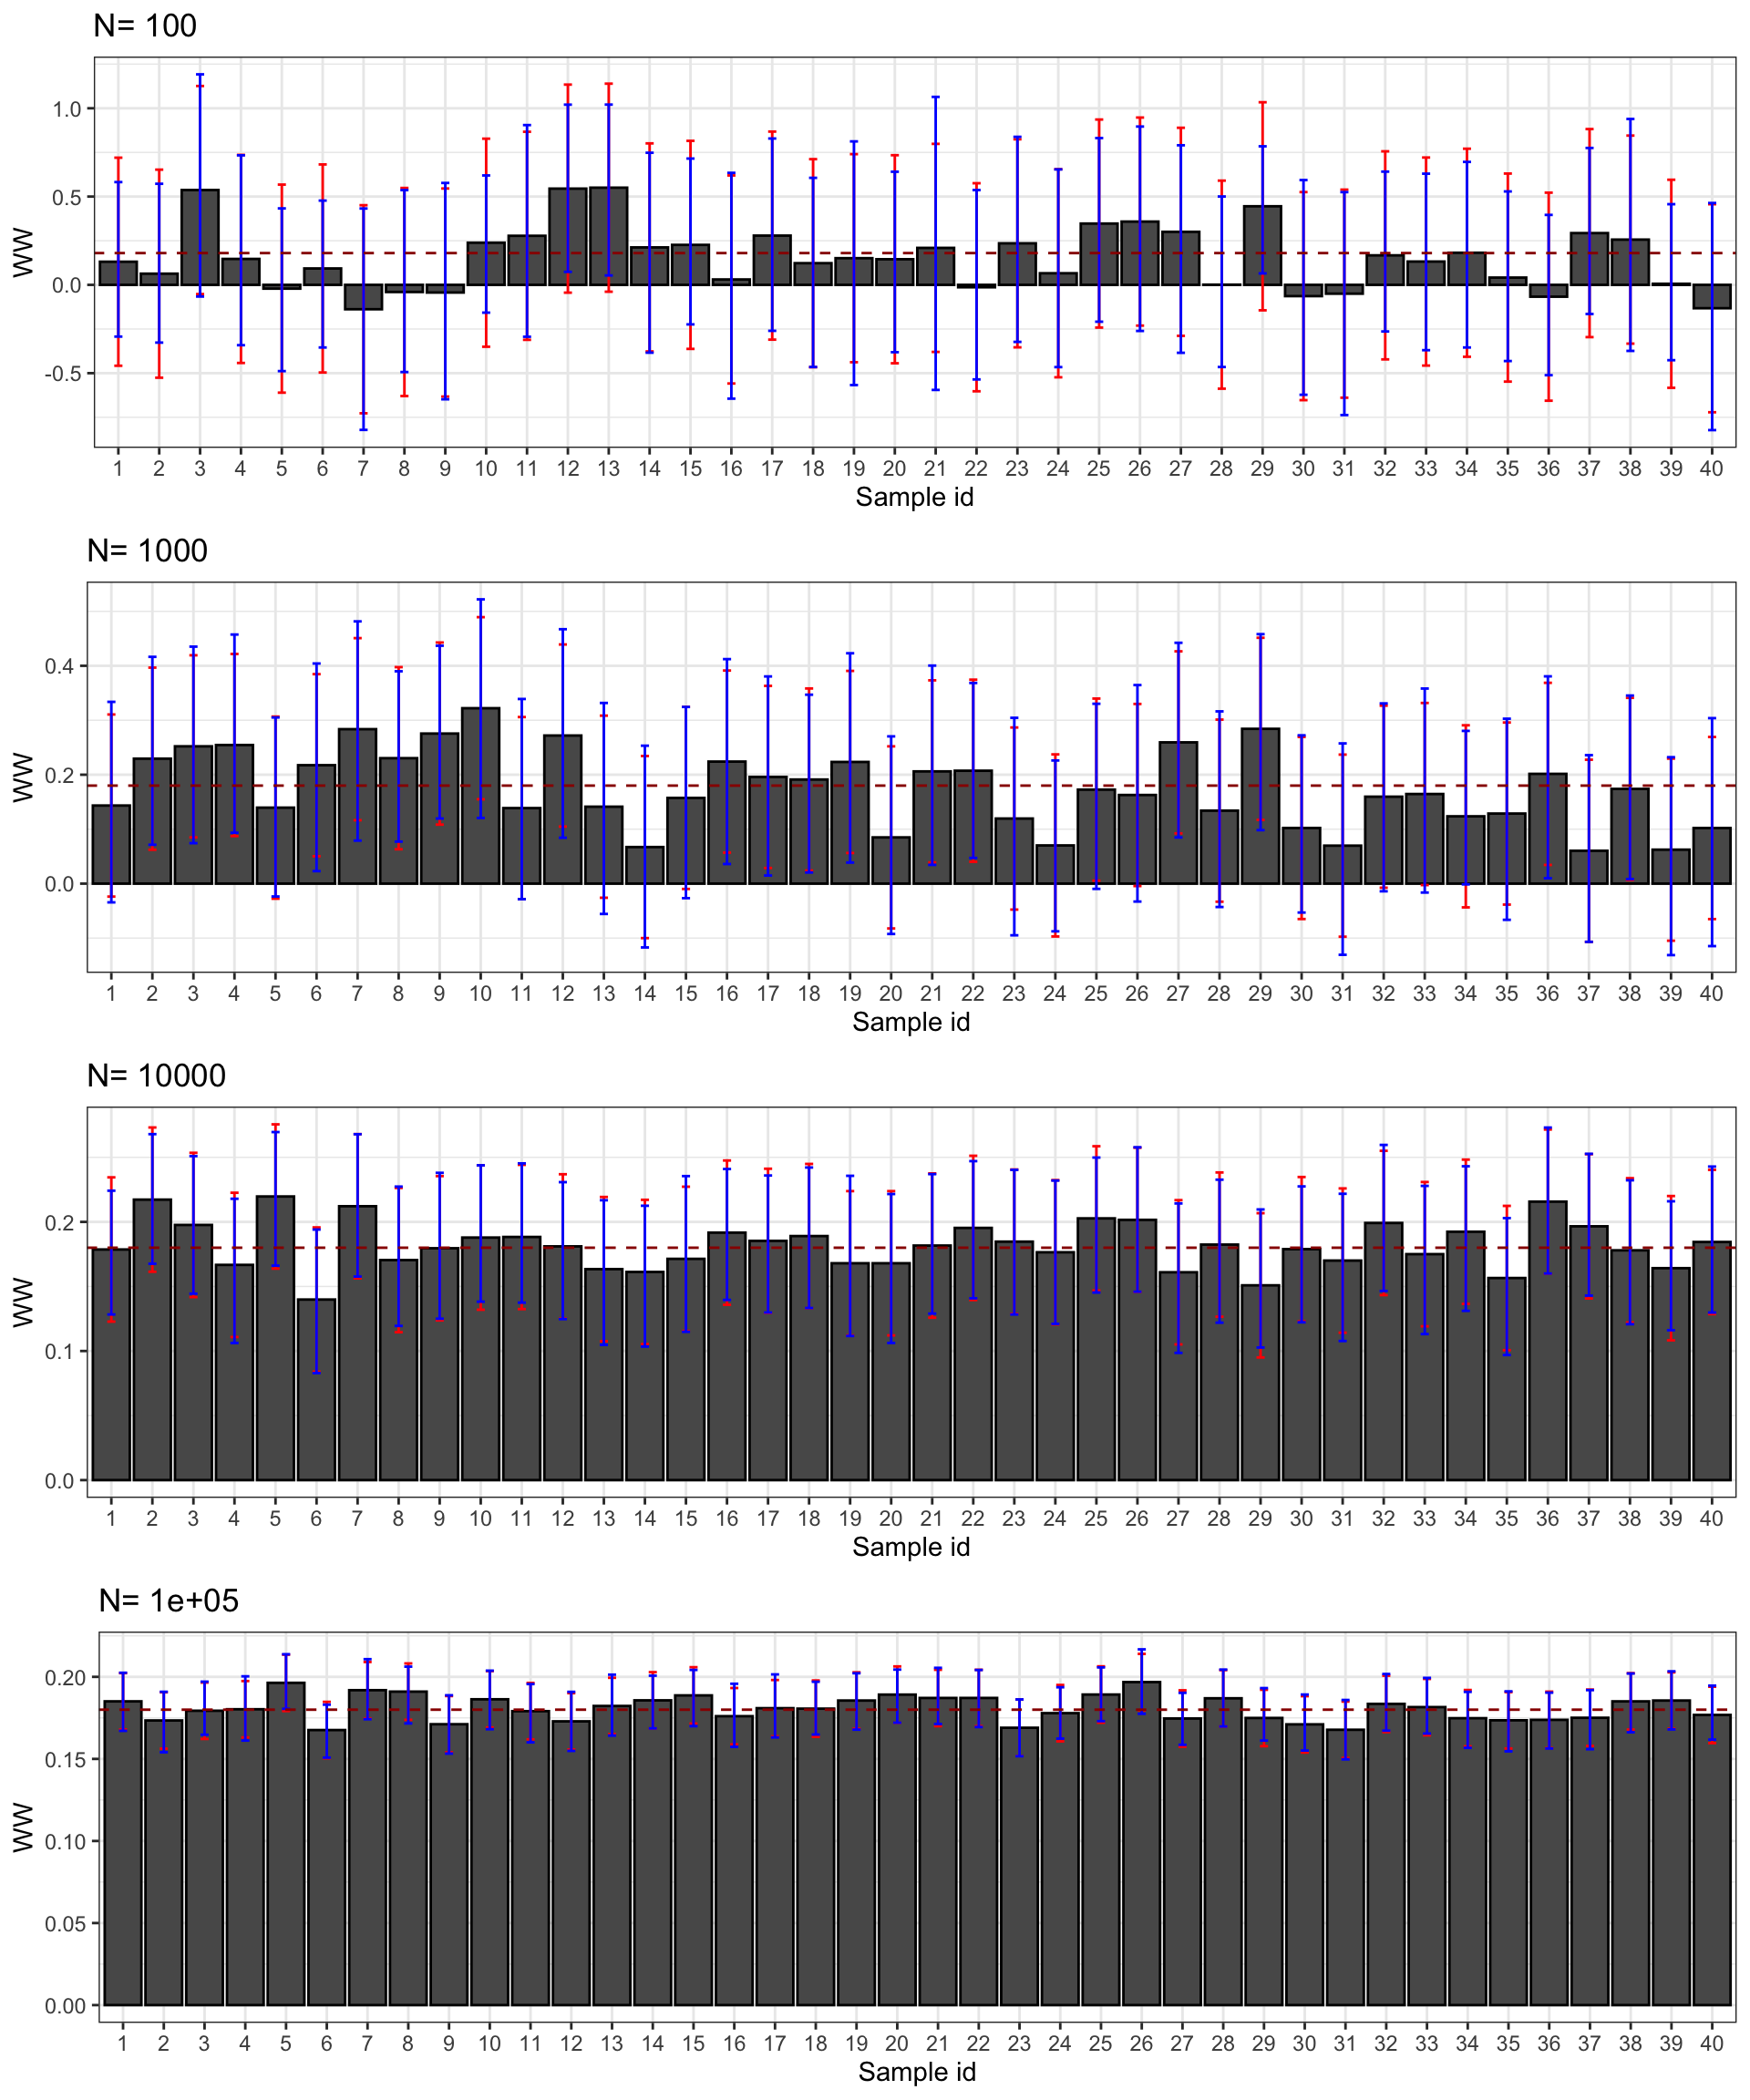
\includegraphics[width=0.6\linewidth]{STCI_files/figure-latex/confintervalboot-1} 

}

\caption{Bootstrapped confidence intervals of $\hat{WW}$ for $\delta=$ 0.99 over sample replications for various sample sizes (true confidence intervals in red)}\label{fig:confintervalboot}
\end{figure}

\textbf{TO DO: COMMENT AND USE PIVOTAL TEST STATISTIC}

\subsubsection{Randomization inference}\label{randomization-inference}

Randomization inference (a.k.a. Fisher's permutation approach) tries to
mimick the sampling noise due to the random allocation of the treatment
vector, as we have seen in Section \ref{sec:illusnoisesamp}. In
practice, the idea is simply to look at how the treatment effect that we
estimate varies when we visit all the possible allocations of the
treament dummy in the sample. For each new allocation, we are going to
compute the with/without estimator using the observed outcomes and the
newly allocated treatment dummy. It means that some actually treated
observations are going to enter into the computation of the control
group mean, while some actually untreated observations are going to
enter into the computation of the treatment group mean. As a
consequence, the resulting distribution will be centered at zero. Under
the assumption of a constant treatment effect, the distribution of the
parameter obtained using randomization inference will be an exact
estimation of sampling noise for the sample treatment effect.

Notice how beautilful the result is: randomization inference yields an
\textbf{exact} measure of sampling noise. The resulting estimate of
sampling noise is not an approximation that is going to become better as
sample size increases. No, it is the \textbf{actual} value of sampling
noise in the sample.

There are two ways to compute a confidence interval using Fisher's
permutation approach. One is to form symmetric intervals using our
estimate of sampling noise as presented in Section \ref{sec:confinterv}.
Another approach is to directly use the quantiles of the distribution of
the parameter centered around the estimated treatment effect, in the
same spirit as bootstrapped confidence intervals using the percentile
approach. This last approach accomodates possible asymetries in the
finite sample distribution of the treatment effect.

Computing the value of the treatment effect for all possible treatment
allocations can take a lot of time with large samples. That's why we in
general compute the test statistic for a reasonably large number of
random allocations.

\BeginKnitrBlock{remark}
\iffalse{} {Remark. } \fi{}Fisher's original approach is slightly
different from the one I delineate here. Fisher wanted to derive a test
statistic for whether the treatment effect was zero, not to estimate
sampling noise. Under the null that the treatment has absolutely no
effect whatsoever on any unit, any test statistic whose value should be
zero if the two distributions where identical can be computed on the
actual sample and its distribution can be derived using Fisher's
permutation approach. The test statistic can be the difference in means,
standard deviations, medians, ranks, the T-stat, the Kolmogorov-Smirnov
test statistic or any other test statistic that you might want to
compute. Comparing the actual value of the test statistic to its
distribution under the null gives a p-value for the validity of the
null.
\EndKnitrBlock{remark}

\BeginKnitrBlock{remark}
\iffalse{} {Remark. } \fi{}Imbens and Rubin propose a more complex
procedure to derive the confidence interval for the treatment effect
using randomization inference. They propose to compute Fisher's p-value
for different values of the treatment effect, and to set the confidence
interval as the values of the treatment effect under and above which the
p-value is smaller than \(\delta\). When using the with/without
estimator as the test statistic, the two approches should be equivalent.
Is is possible that the estimates using statistics less influenced by
outliers are more precise though.
\EndKnitrBlock{remark}

\BeginKnitrBlock{remark}
\iffalse{} {Remark. } \fi{}Note that we pay two prices for having an
exact estimation of sampling noise:
\EndKnitrBlock{remark}

\begin{enumerate}
\def\labelenumi{\arabic{enumi}.}
\tightlist
\item
  We have to assume that the treatment effect is constant, e.g.~we have
  to assume homoskedasticity. This is in general not the case. Whether
  this is in general a big issue depends on how large the difference is
  between homoskedastic and heteroskedastic standard errors. One way
  around this issue would be to add a small amount of noise to the
  observations that are in the group with the lowest variance. Whether
  this would work in practice is still to be demonstrated.
\item
  We have to be interested only in the sampling noise of the sample
  treatment effect. The sampling noise of the population treatment
  effect is not estimated using Fisher's permutation approach. As we
  have seen in Section \ref{sec:illusnoisesamp}, there is no practical
  difference between these two sampling noises in our example. Whether
  this is the case in general deserves further investigation.
\end{enumerate}

\BeginKnitrBlock{example}
\protect\hypertarget{exm:unnamed-chunk-63}{}{\label{exm:unnamed-chunk-63}
}In practice, randomization inference is very close to a bootstrap
procedure, except that instead of resampling with replacement from the
original sample, we only change the vector of treatment allocation at
each replication.
\EndKnitrBlock{example}

\begin{Shaded}
\begin{Highlighting}[]
\NormalTok{fisher.fun.ww.}\DecValTok{1}\NormalTok{ <-}\StringTok{ }\ControlFlowTok{function}\NormalTok{(seed,data)\{}
  \KeywordTok{set.seed}\NormalTok{(seed,}\DataTypeTok{kind=}\StringTok{"Wichmann-Hill"}\NormalTok{)}
\NormalTok{  data}\OperatorTok{$}\NormalTok{D <-}\StringTok{ }\KeywordTok{rbinom}\NormalTok{(}\KeywordTok{nrow}\NormalTok{(data),}\DecValTok{1}\NormalTok{,}\KeywordTok{mean}\NormalTok{(data}\OperatorTok{$}\NormalTok{Ds))}
\NormalTok{  ols.ww <-}\StringTok{ }\KeywordTok{lm}\NormalTok{(y}\OperatorTok{~}\NormalTok{D,}\DataTypeTok{data=}\NormalTok{data)}
\NormalTok{  ww <-}\StringTok{ }\NormalTok{ols.ww}\OperatorTok{$}\NormalTok{coef[[}\DecValTok{2}\NormalTok{]]}
  \KeywordTok{return}\NormalTok{(ww)}
\NormalTok{\}}

\NormalTok{fisher.fun.ww <-}\StringTok{ }\ControlFlowTok{function}\NormalTok{(Nfisher,data,delta)\{}
\NormalTok{  fisher <-}\StringTok{ }\KeywordTok{unlist}\NormalTok{(}\KeywordTok{lapply}\NormalTok{(}\DecValTok{1}\OperatorTok{:}\NormalTok{Nfisher,fisher.fun.ww.}\DecValTok{1}\NormalTok{,}\DataTypeTok{data=}\NormalTok{data))}
\NormalTok{  ols.ww <-}\StringTok{ }\KeywordTok{lm}\NormalTok{(y}\OperatorTok{~}\NormalTok{Ds,}\DataTypeTok{data=}\NormalTok{data)}
\NormalTok{  ww <-}\StringTok{ }\NormalTok{ols.ww}\OperatorTok{$}\NormalTok{coef[[}\DecValTok{2}\NormalTok{]]}
\NormalTok{  fisher <-}\StringTok{ }\NormalTok{fisher}\OperatorTok{+}\StringTok{ }\NormalTok{ww}
\NormalTok{  fisher.CI.ww <-}\StringTok{ }\KeywordTok{c}\NormalTok{(}\KeywordTok{quantile}\NormalTok{(fisher,}\DataTypeTok{prob=}\NormalTok{(}\DecValTok{1}\OperatorTok{-}\NormalTok{delta)}\OperatorTok{/}\DecValTok{2}\NormalTok{),}\KeywordTok{quantile}\NormalTok{(fisher,}\DataTypeTok{prob=}\NormalTok{(}\DecValTok{1}\OperatorTok{+}\NormalTok{delta)}\OperatorTok{/}\DecValTok{2}\NormalTok{))}
\NormalTok{  fisher.samp.noise.ww <-}\StringTok{ }\KeywordTok{quantile}\NormalTok{(fisher,}\DataTypeTok{prob=}\NormalTok{(}\DecValTok{1}\OperatorTok{+}\NormalTok{delta)}\OperatorTok{/}\DecValTok{2}\NormalTok{)}\OperatorTok{-}\KeywordTok{quantile}\NormalTok{(fisher,}\DataTypeTok{prob=}\NormalTok{(}\DecValTok{1}\OperatorTok{-}\NormalTok{delta)}\OperatorTok{/}\DecValTok{2}\NormalTok{)}
  \KeywordTok{return}\NormalTok{(}\KeywordTok{list}\NormalTok{(fisher,fisher.CI.ww,fisher.samp.noise.ww))}
\NormalTok{\}}

\NormalTok{Nfisher <-}\StringTok{ }\DecValTok{500}
\NormalTok{ww.fisher <-}\StringTok{ }\KeywordTok{fisher.fun.ww}\NormalTok{(Nfisher,data,delta)}
\end{Highlighting}
\end{Shaded}

Over 500 replications, the 99\% confidence interval based on Fisher's
permutation approach is \(\left\{-0.052;0.3\right\}\). As a consequence,
the bootstrapped estimate of 99\% sampling noise is of 0.352. Remember
that, with \(N=\) 1000, sampling noise is actually equal to 0.39.

In order to assess the global precision of Fisher's permutation method,
we are going to resort to Monte Carlo simulations.

\begin{Shaded}
\begin{Highlighting}[]
\NormalTok{monte.carlo.ww.fisher <-}\StringTok{ }\ControlFlowTok{function}\NormalTok{(s,N,param,Nfisher,delta)\{}
  \KeywordTok{set.seed}\NormalTok{(s)}
\NormalTok{  mu <-}\StringTok{ }\KeywordTok{rnorm}\NormalTok{(N,param[}\StringTok{"barmu"}\NormalTok{],}\KeywordTok{sqrt}\NormalTok{(param[}\StringTok{"sigma2mu"}\NormalTok{]))}
\NormalTok{  UB <-}\StringTok{ }\KeywordTok{rnorm}\NormalTok{(N,}\DecValTok{0}\NormalTok{,}\KeywordTok{sqrt}\NormalTok{(param[}\StringTok{"sigma2U"}\NormalTok{]))}
\NormalTok{  yB <-}\StringTok{ }\NormalTok{mu }\OperatorTok{+}\StringTok{ }\NormalTok{UB }
\NormalTok{  YB <-}\StringTok{ }\KeywordTok{exp}\NormalTok{(yB)}
\NormalTok{  Ds <-}\StringTok{ }\KeywordTok{rep}\NormalTok{(}\DecValTok{0}\NormalTok{,N)}
\NormalTok{  V <-}\StringTok{ }\KeywordTok{rnorm}\NormalTok{(N,param[}\StringTok{"barmu"}\NormalTok{],}\KeywordTok{sqrt}\NormalTok{(param[}\StringTok{"sigma2mu"}\NormalTok{]}\OperatorTok{+}\NormalTok{param[}\StringTok{"sigma2U"}\NormalTok{]))}
\NormalTok{  Ds[V}\OperatorTok{<=}\KeywordTok{log}\NormalTok{(param[}\StringTok{"barY"}\NormalTok{])] <-}\StringTok{ }\DecValTok{1} 
\NormalTok{  epsilon <-}\StringTok{ }\KeywordTok{rnorm}\NormalTok{(N,}\DecValTok{0}\NormalTok{,}\KeywordTok{sqrt}\NormalTok{(param[}\StringTok{"sigma2epsilon"}\NormalTok{]))}
\NormalTok{  eta<-}\StringTok{ }\KeywordTok{rnorm}\NormalTok{(N,}\DecValTok{0}\NormalTok{,}\KeywordTok{sqrt}\NormalTok{(param[}\StringTok{"sigma2eta"}\NormalTok{]))}
\NormalTok{  U0 <-}\StringTok{ }\NormalTok{param[}\StringTok{"rho"}\NormalTok{]}\OperatorTok{*}\NormalTok{UB }\OperatorTok{+}\StringTok{ }\NormalTok{epsilon}
\NormalTok{  y0 <-}\StringTok{ }\NormalTok{mu }\OperatorTok{+}\StringTok{  }\NormalTok{U0 }\OperatorTok{+}\StringTok{ }\NormalTok{param[}\StringTok{"delta"}\NormalTok{]}
\NormalTok{  alpha <-}\StringTok{ }\NormalTok{param[}\StringTok{"baralpha"}\NormalTok{]}\OperatorTok{+}\StringTok{  }\NormalTok{param[}\StringTok{"theta"}\NormalTok{]}\OperatorTok{*}\NormalTok{mu }\OperatorTok{+}\StringTok{ }\NormalTok{eta}
\NormalTok{  y1 <-}\StringTok{ }\NormalTok{y0}\OperatorTok{+}\NormalTok{alpha}
\NormalTok{  Y0 <-}\StringTok{ }\KeywordTok{exp}\NormalTok{(y0)}
\NormalTok{  Y1 <-}\StringTok{ }\KeywordTok{exp}\NormalTok{(y1)}
\NormalTok{  y <-}\StringTok{ }\NormalTok{y1}\OperatorTok{*}\NormalTok{Ds}\OperatorTok{+}\NormalTok{y0}\OperatorTok{*}\NormalTok{(}\DecValTok{1}\OperatorTok{-}\NormalTok{Ds)}
\NormalTok{  Y <-}\StringTok{ }\NormalTok{Y1}\OperatorTok{*}\NormalTok{Ds}\OperatorTok{+}\NormalTok{Y0}\OperatorTok{*}\NormalTok{(}\DecValTok{1}\OperatorTok{-}\NormalTok{Ds)}
\NormalTok{  data <-}\StringTok{ }\KeywordTok{as.data.frame}\NormalTok{(}\KeywordTok{cbind}\NormalTok{(y,Ds,yB))}
\NormalTok{  ww.fisher <-}\StringTok{ }\KeywordTok{fisher.fun.ww}\NormalTok{(Nfisher,data,delta)}
  \KeywordTok{return}\NormalTok{(}\KeywordTok{c}\NormalTok{((}\DecValTok{1}\OperatorTok{/}\KeywordTok{sum}\NormalTok{(Ds))}\OperatorTok{*}\KeywordTok{sum}\NormalTok{(y}\OperatorTok{*}\NormalTok{Ds)}\OperatorTok{-}\NormalTok{(}\DecValTok{1}\OperatorTok{/}\KeywordTok{sum}\NormalTok{(}\DecValTok{1}\OperatorTok{-}\NormalTok{Ds))}\OperatorTok{*}\KeywordTok{sum}\NormalTok{(y}\OperatorTok{*}\NormalTok{(}\DecValTok{1}\OperatorTok{-}\NormalTok{Ds)),}\KeywordTok{var}\NormalTok{(y[Ds}\OperatorTok{==}\DecValTok{1}\NormalTok{]),}\KeywordTok{var}\NormalTok{(y[Ds}\OperatorTok{==}\DecValTok{0}\NormalTok{]),}\KeywordTok{mean}\NormalTok{(Ds),ww.fisher[[}\DecValTok{2}\NormalTok{]][}\DecValTok{1}\NormalTok{],ww.fisher[[}\DecValTok{2}\NormalTok{]][}\DecValTok{2}\NormalTok{],ww.fisher[[}\DecValTok{3}\NormalTok{]]))}
\NormalTok{\}}

\NormalTok{sf.simuls.ww.N.fisher <-}\StringTok{ }\ControlFlowTok{function}\NormalTok{(N,Nsim,Nfisher,delta,param)\{}
  \KeywordTok{sfInit}\NormalTok{(}\DataTypeTok{parallel=}\OtherTok{TRUE}\NormalTok{,}\DataTypeTok{cpus=}\DecValTok{2}\OperatorTok{*}\NormalTok{ncpus)}
  \KeywordTok{sfExport}\NormalTok{(}\StringTok{"fisher.fun.ww"}\NormalTok{,}\StringTok{"fisher.fun.ww.1"}\NormalTok{)}
\NormalTok{  sim <-}\StringTok{ }\KeywordTok{as.data.frame}\NormalTok{(}\KeywordTok{matrix}\NormalTok{(}\KeywordTok{unlist}\NormalTok{(}\KeywordTok{sfLapply}\NormalTok{(}\DecValTok{1}\OperatorTok{:}\NormalTok{Nsim,monte.carlo.ww.fisher,}\DataTypeTok{N=}\NormalTok{N,}\DataTypeTok{Nfisher=}\NormalTok{Nfisher,}\DataTypeTok{delta=}\NormalTok{delta,}\DataTypeTok{param=}\NormalTok{param)),}\DataTypeTok{nrow=}\NormalTok{Nsim,}\DataTypeTok{ncol=}\DecValTok{7}\NormalTok{,}\DataTypeTok{byrow=}\OtherTok{TRUE}\NormalTok{))}
  \KeywordTok{sfStop}\NormalTok{()}
  \KeywordTok{colnames}\NormalTok{(sim) <-}\StringTok{ }\KeywordTok{c}\NormalTok{(}\StringTok{'WW'}\NormalTok{,}\StringTok{'V1'}\NormalTok{,}\StringTok{'V0'}\NormalTok{,}\StringTok{'p'}\NormalTok{,}\StringTok{'fisher.lCI'}\NormalTok{,}\StringTok{'fisher.uCI'}\NormalTok{,}\StringTok{'fisher.samp.noise'}\NormalTok{)}
  \KeywordTok{return}\NormalTok{(sim)}
\NormalTok{\}}

\NormalTok{simuls.ww.fisher <-}\StringTok{ }\KeywordTok{lapply}\NormalTok{(N.sample,sf.simuls.ww.N.fisher,}\DataTypeTok{Nsim=}\NormalTok{Nsim,}\DataTypeTok{param=}\NormalTok{param,}\DataTypeTok{Nfisher=}\NormalTok{Nfisher,}\DataTypeTok{delta=}\NormalTok{delta)}
\end{Highlighting}
\end{Shaded}

We can now graph our bootstrapped estimate of sampling noise in all of
our samples, the average bootstrapped estimates of sampling noise and of
confidence intervals, as Figures \ref{fig:sampnoisewwfisherall},
\ref{fig:sampnoisewwfisherplot} and \ref{fig:confintervalfisher} show.
The results are pretty good. On average, estimates of sampling noise
using Randomization Inference are pretty accurate, as Figure
\ref{fig:sampnoisewwfisherplot} shows. It seems that sampling noise is
underestimated by Randomization Inference when \(N=\) 1000, without any
clear reason why.

\begin{Shaded}
\begin{Highlighting}[]
\KeywordTok{par}\NormalTok{(}\DataTypeTok{mfrow=}\KeywordTok{c}\NormalTok{(}\DecValTok{2}\NormalTok{,}\DecValTok{2}\NormalTok{))}
\ControlFlowTok{for}\NormalTok{ (i }\ControlFlowTok{in} \DecValTok{1}\OperatorTok{:}\DecValTok{4}\NormalTok{)\{}
  \KeywordTok{hist}\NormalTok{(simuls.ww.fisher[[i]][,}\StringTok{'fisher.samp.noise'}\NormalTok{],}\DataTypeTok{main=}\KeywordTok{paste}\NormalTok{(}\StringTok{'N='}\NormalTok{,}\KeywordTok{as.character}\NormalTok{(N.sample[i])),}\DataTypeTok{xlab=}\KeywordTok{expression}\NormalTok{(}\KeywordTok{hat}\NormalTok{(}\DecValTok{2}\OperatorTok{*}\KeywordTok{bar}\NormalTok{(epsilon))),}\DataTypeTok{xlim=}\KeywordTok{c}\NormalTok{(}\KeywordTok{min}\NormalTok{(simuls.ww.fisher[[i]][,}\StringTok{'fisher.samp.noise'}\NormalTok{]),}\KeywordTok{max}\NormalTok{(simuls.ww.fisher[[i]][,}\StringTok{'fisher.samp.noise'}\NormalTok{])))}
  \KeywordTok{abline}\NormalTok{(}\DataTypeTok{v=}\NormalTok{table.noise[i,}\KeywordTok{colnames}\NormalTok{(table.noise)}\OperatorTok{==}\StringTok{'sampling.noise'}\NormalTok{],}\DataTypeTok{col=}\StringTok{"red"}\NormalTok{)}
\NormalTok{\}}
\end{Highlighting}
\end{Shaded}

\begin{figure}[htbp]

{\centering 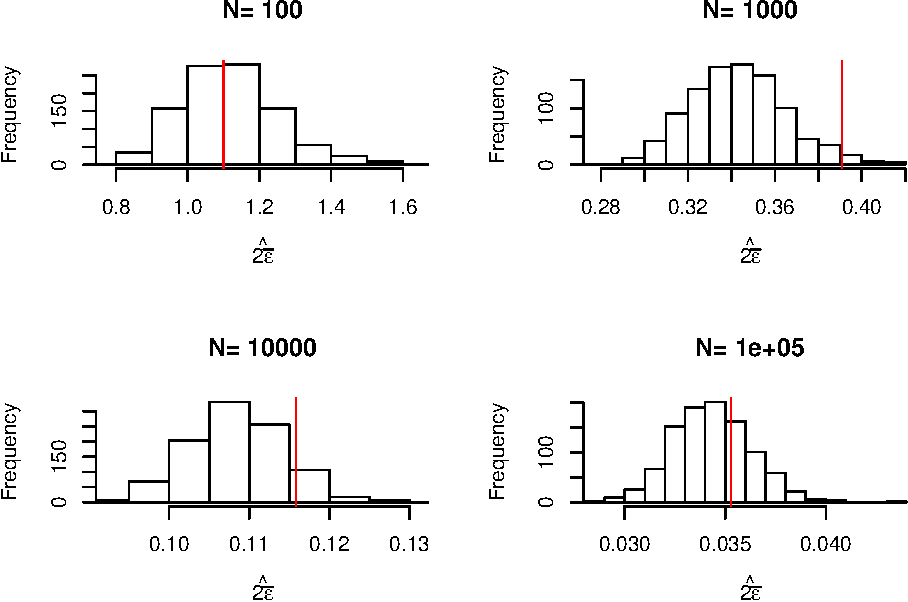
\includegraphics[width=0.6\linewidth]{STCI_files/figure-latex/sampnoisewwfisherall-1} 

}

\caption{Distribution of the estimates of sampling noise using Randomization Inference over replications of samples of different sizes (true sampling noise in red)}\label{fig:sampnoisewwfisherall}
\end{figure}

\begin{Shaded}
\begin{Highlighting}[]
\ControlFlowTok{for}\NormalTok{ (k }\ControlFlowTok{in}\NormalTok{ (}\DecValTok{1}\OperatorTok{:}\KeywordTok{length}\NormalTok{(N.sample)))\{}
\NormalTok{  table.noise}\OperatorTok{$}\NormalTok{fisher.noise[k] <-}\StringTok{ }\KeywordTok{mean}\NormalTok{(simuls.ww.fisher[[k]]}\OperatorTok{$}\NormalTok{fisher.samp.noise)}
\NormalTok{\}}
\KeywordTok{ggplot}\NormalTok{(table.noise, }\KeywordTok{aes}\NormalTok{(}\DataTypeTok{x=}\KeywordTok{as.factor}\NormalTok{(N), }\DataTypeTok{y=}\NormalTok{TT)) }\OperatorTok{+}
\StringTok{  }\KeywordTok{geom_bar}\NormalTok{(}\DataTypeTok{position=}\KeywordTok{position_dodge}\NormalTok{(), }\DataTypeTok{stat=}\StringTok{"identity"}\NormalTok{, }\DataTypeTok{colour=}\StringTok{'black'}\NormalTok{) }\OperatorTok{+}
\StringTok{  }\KeywordTok{geom_errorbar}\NormalTok{(}\KeywordTok{aes}\NormalTok{(}\DataTypeTok{ymin=}\NormalTok{TT}\OperatorTok{-}\NormalTok{sampling.noise}\OperatorTok{/}\DecValTok{2}\NormalTok{, }\DataTypeTok{ymax=}\NormalTok{TT}\OperatorTok{+}\NormalTok{sampling.noise}\OperatorTok{/}\DecValTok{2}\NormalTok{), }\DataTypeTok{width=}\NormalTok{.}\DecValTok{2}\NormalTok{,}\DataTypeTok{position=}\KeywordTok{position_dodge}\NormalTok{(.}\DecValTok{9}\NormalTok{),}\DataTypeTok{color=}\StringTok{'red'}\NormalTok{) }\OperatorTok{+}
\StringTok{  }\KeywordTok{geom_errorbar}\NormalTok{(}\KeywordTok{aes}\NormalTok{(}\DataTypeTok{ymin=}\NormalTok{TT}\OperatorTok{-}\NormalTok{fisher.noise}\OperatorTok{/}\DecValTok{2}\NormalTok{, }\DataTypeTok{ymax=}\NormalTok{TT}\OperatorTok{+}\NormalTok{fisher.noise}\OperatorTok{/}\DecValTok{2}\NormalTok{), }\DataTypeTok{width=}\NormalTok{.}\DecValTok{2}\NormalTok{,}\DataTypeTok{position=}\KeywordTok{position_dodge}\NormalTok{(.}\DecValTok{9}\NormalTok{),}\DataTypeTok{color=}\StringTok{'blue'}\NormalTok{) }\OperatorTok{+}
\StringTok{  }\KeywordTok{xlab}\NormalTok{(}\StringTok{"Sample Size"}\NormalTok{)}\OperatorTok{+}
\StringTok{  }\KeywordTok{theme_bw}\NormalTok{()}
\end{Highlighting}
\end{Shaded}

\begin{figure}[htbp]

{\centering 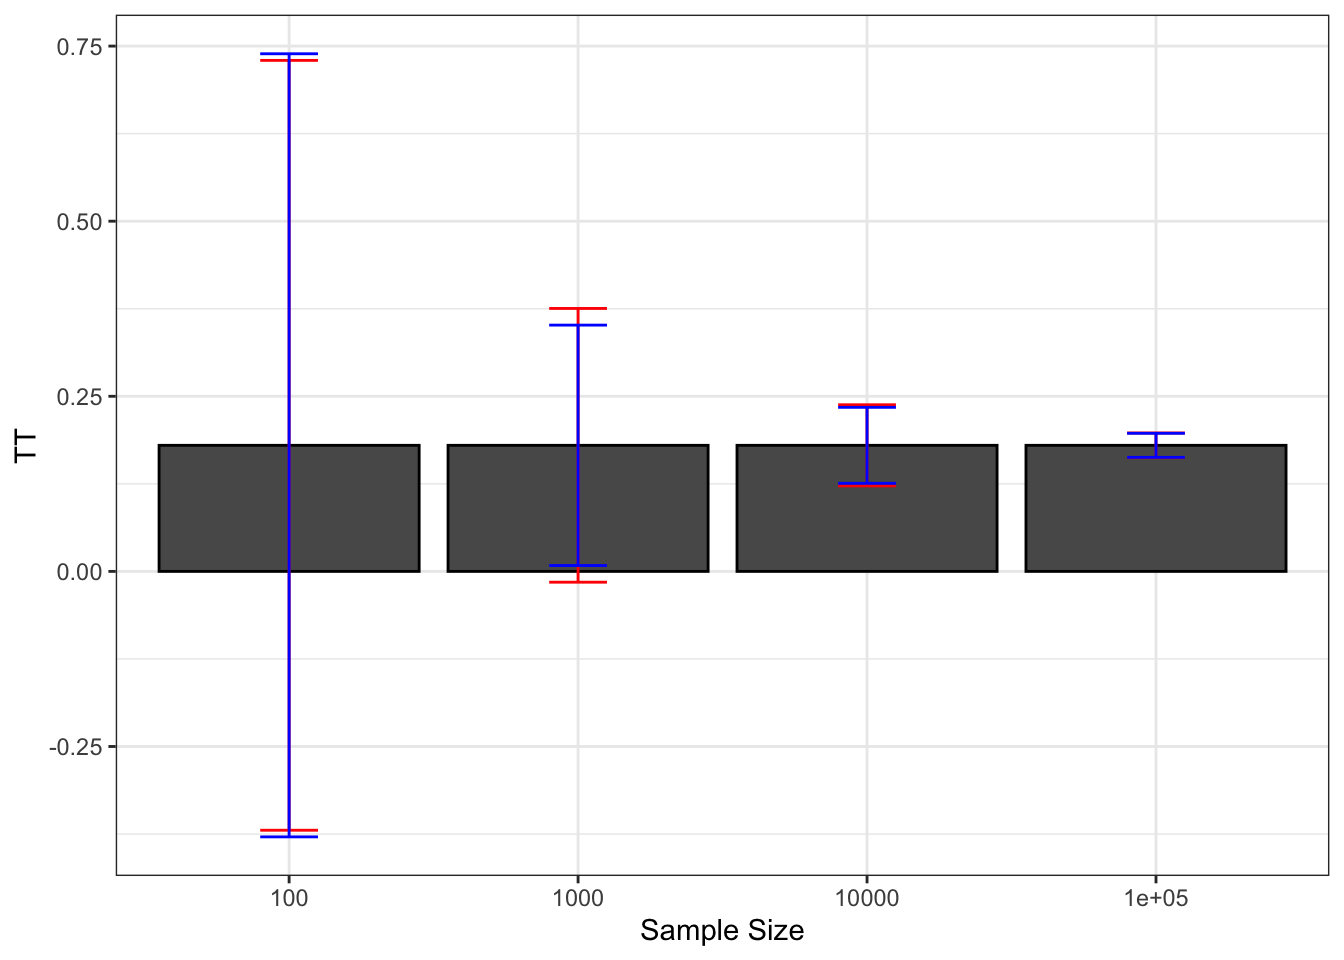
\includegraphics[width=0.6\linewidth]{STCI_files/figure-latex/sampnoisewwfisherplot-1} 

}

\caption{Average estimates of sampling noise using Randomization Inference over replications of samples of different sizes (true sampling noise in red)}\label{fig:sampnoisewwfisherplot}
\end{figure}

\begin{Shaded}
\begin{Highlighting}[]
\NormalTok{N.plot <-}\StringTok{ }\DecValTok{40}
\NormalTok{plot.list <-}\StringTok{ }\KeywordTok{list}\NormalTok{()}

\ControlFlowTok{for}\NormalTok{ (k }\ControlFlowTok{in} \DecValTok{1}\OperatorTok{:}\KeywordTok{length}\NormalTok{(N.sample))\{}
 \KeywordTok{set.seed}\NormalTok{(}\DecValTok{1234}\NormalTok{)}
\NormalTok{ test.fisher <-}\StringTok{ }\NormalTok{simuls.ww.fisher[[k]][}\KeywordTok{sample}\NormalTok{(N.plot),}\KeywordTok{c}\NormalTok{(}\StringTok{'WW'}\NormalTok{,}\StringTok{'fisher.lCI'}\NormalTok{,}\StringTok{'fisher.uCI'}\NormalTok{)]}
\NormalTok{ test.fisher <-}\StringTok{ }\KeywordTok{as.data.frame}\NormalTok{(}\KeywordTok{cbind}\NormalTok{(test.fisher,}\KeywordTok{rep}\NormalTok{(}\KeywordTok{samp.noise}\NormalTok{(simuls.ww.fisher[[k]][,}\StringTok{'WW'}\NormalTok{],}\DataTypeTok{delta=}\NormalTok{delta),N.plot)))}
 \KeywordTok{colnames}\NormalTok{(test.fisher) <-}\StringTok{ }\KeywordTok{c}\NormalTok{(}\StringTok{'WW'}\NormalTok{,}\StringTok{'fisher.lCI'}\NormalTok{,}\StringTok{'fisher.uCI'}\NormalTok{,}\StringTok{'sampling.noise'}\NormalTok{)}
\NormalTok{ test.fisher}\OperatorTok{$}\NormalTok{id <-}\StringTok{ }\DecValTok{1}\OperatorTok{:}\NormalTok{N.plot}
\NormalTok{ plot.test.fisher <-}\StringTok{ }\KeywordTok{ggplot}\NormalTok{(test.fisher, }\KeywordTok{aes}\NormalTok{(}\DataTypeTok{x=}\KeywordTok{as.factor}\NormalTok{(id), }\DataTypeTok{y=}\NormalTok{WW)) }\OperatorTok{+}
\StringTok{     }\KeywordTok{geom_bar}\NormalTok{(}\DataTypeTok{position=}\KeywordTok{position_dodge}\NormalTok{(), }\DataTypeTok{stat=}\StringTok{"identity"}\NormalTok{, }\DataTypeTok{colour=}\StringTok{'black'}\NormalTok{) }\OperatorTok{+}
\StringTok{     }\KeywordTok{geom_errorbar}\NormalTok{(}\KeywordTok{aes}\NormalTok{(}\DataTypeTok{ymin=}\NormalTok{WW}\OperatorTok{-}\NormalTok{sampling.noise}\OperatorTok{/}\DecValTok{2}\NormalTok{, }\DataTypeTok{ymax=}\NormalTok{WW}\OperatorTok{+}\NormalTok{sampling.noise}\OperatorTok{/}\DecValTok{2}\NormalTok{), }\DataTypeTok{width=}\NormalTok{.}\DecValTok{2}\NormalTok{,}\DataTypeTok{position=}\KeywordTok{position_dodge}\NormalTok{(.}\DecValTok{9}\NormalTok{),}\DataTypeTok{color=}\StringTok{'red'}\NormalTok{) }\OperatorTok{+}
\StringTok{     }\KeywordTok{geom_errorbar}\NormalTok{(}\KeywordTok{aes}\NormalTok{(}\DataTypeTok{ymin=}\NormalTok{fisher.lCI, }\DataTypeTok{ymax=}\NormalTok{fisher.uCI), }\DataTypeTok{width=}\NormalTok{.}\DecValTok{2}\NormalTok{,}\DataTypeTok{position=}\KeywordTok{position_dodge}\NormalTok{(.}\DecValTok{9}\NormalTok{),}\DataTypeTok{color=}\StringTok{'blue'}\NormalTok{) }\OperatorTok{+}
\StringTok{     }\KeywordTok{geom_hline}\NormalTok{(}\KeywordTok{aes}\NormalTok{(}\DataTypeTok{yintercept=}\KeywordTok{delta.y.ate}\NormalTok{(param)), }\DataTypeTok{colour=}\StringTok{"#990000"}\NormalTok{, }\DataTypeTok{linetype=}\StringTok{"dashed"}\NormalTok{)}\OperatorTok{+}
\StringTok{     }\KeywordTok{xlab}\NormalTok{(}\StringTok{"Sample id"}\NormalTok{)}\OperatorTok{+}
\StringTok{     }\KeywordTok{theme_bw}\NormalTok{()}\OperatorTok{+}
\StringTok{     }\KeywordTok{ggtitle}\NormalTok{(}\KeywordTok{paste}\NormalTok{(}\StringTok{"N="}\NormalTok{,N.sample[k]))}
\NormalTok{ plot.list[[k]] <-}\StringTok{ }\NormalTok{plot.test.fisher}
\NormalTok{\}}
\NormalTok{plot.CI <-}\StringTok{ }\KeywordTok{plot_grid}\NormalTok{(plot.list[[}\DecValTok{1}\NormalTok{]],plot.list[[}\DecValTok{2}\NormalTok{]],plot.list[[}\DecValTok{3}\NormalTok{]],plot.list[[}\DecValTok{4}\NormalTok{]],}\DataTypeTok{ncol=}\DecValTok{1}\NormalTok{,}\DataTypeTok{nrow=}\KeywordTok{length}\NormalTok{(N.sample))}
\KeywordTok{print}\NormalTok{(plot.CI)}
\end{Highlighting}
\end{Shaded}

\begin{figure}[htbp]

{\centering 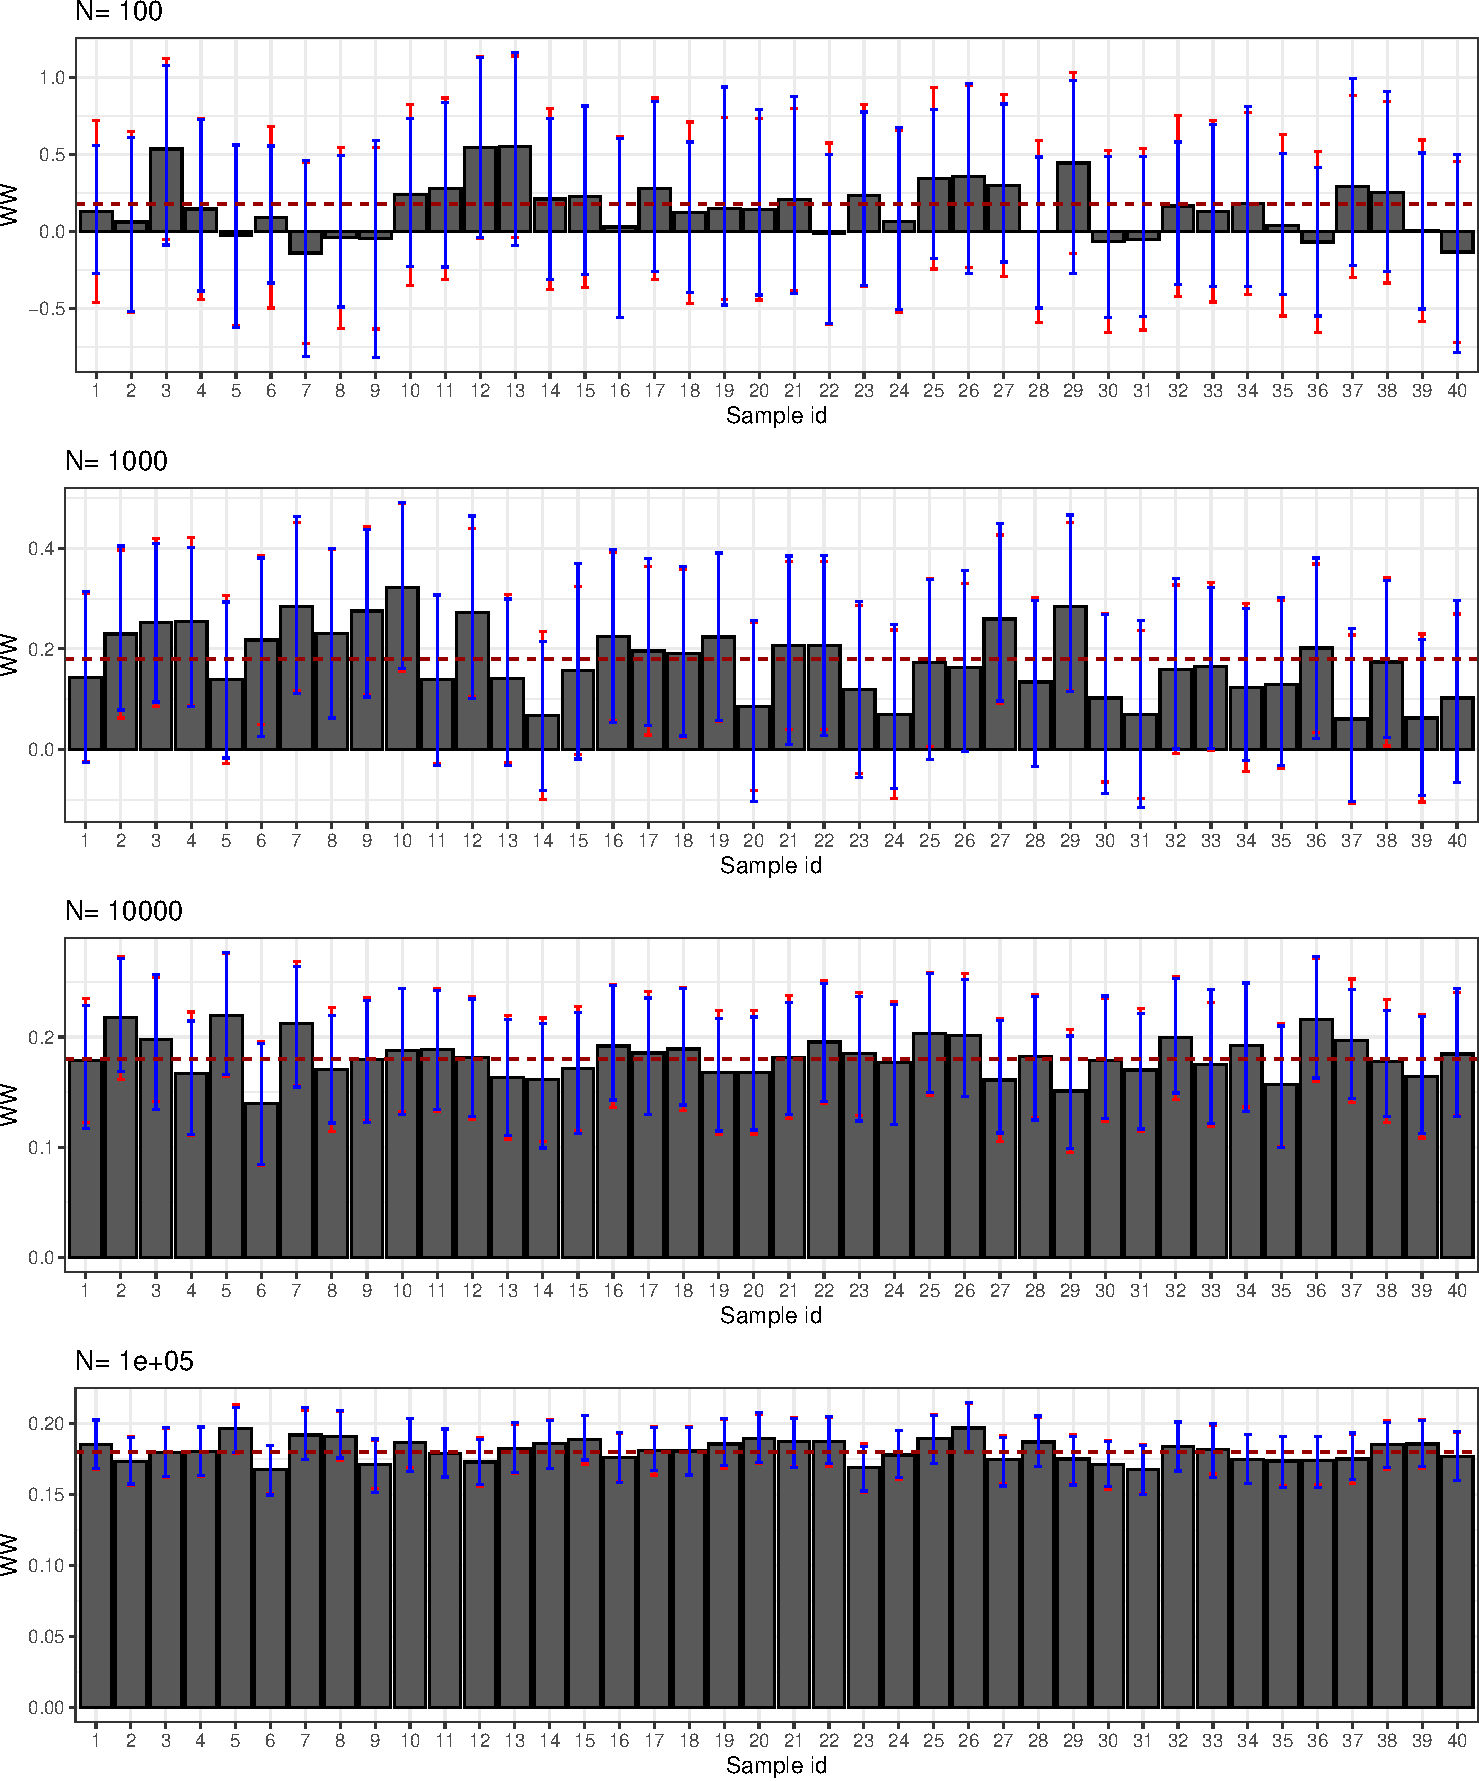
\includegraphics[width=0.6\linewidth]{STCI_files/figure-latex/confintervalfisher-1} 

}

\caption{Confidence intervals of $\hat{WW}$ for $\delta=$ 0.99 estimated using Randomization Inference over sample replications for various sample sizes (true confidence intervals in red)}\label{fig:confintervalfisher}
\end{figure}

\textbf{TO DO: ALTERNATIVE APPROACH USING p-VALUES}

\subsubsection{Subsampling}\label{subsampling}

\textbf{TO DO: ALL}

\part{Methods of Causal
Inference}\label{part-methods-of-causal-inference}

\chapter{Randomized Controlled Trials}\label{RCT}

The most robust and rigorous method that has been devised by social
scientists to estimate the effect of an intervention on an outcome is
the Randomized Controlled Trial (RCT). RCTs are used extensively in the
field to evaluate a wide array of programs, from development, labor and
education interventions to environmental nudges to website and search
engine features.

The key feature of an RCT is the introduction by the researcher of
randomness in the allocation of the treatment. Individuals with
\(R_i=1\), where \(R_i\) denotes the outcome of a random event, such as
a coin toss, have a higher probability of receiving the treatment.
Potential outcomes have the same distribution in both \(R_i=1\) and
\(R_i=0\) groups. If we observe different outcomes between the treatment
and control group, it has to be because of the causal effect of the
treatment, since both groups only differ by the proportion of treated
and controls.

The most attractive feature of RCTs is that researchers enforce the main
identification assumption (we do not have to assume that it holds, we
can make sure that it does). This property of RCTs distinguishes them
from all the other methods that we are going to learn in this class.

In this lecture, we are going to study how to estimate the effect of an
intervention on an outcome using RCTs. We are especially going to study
the various types of designs and what can be recovered from them using
which technique. For each design, we are going to detail which treatment
effect it enables us to identify, how to obtain a sample estimate of
this treatment effect and how to estimate the associated sampling noise.
The main substantial difference between these four designs are the types
of treatment effect parameters that they enable us to recover. Sections
\ref{sec:design1} to \ref{sec:design4} of this lecture introduces the
four designs and how to analyze them.

Unfortunately, RCTs are not bullet proof. They suffer from problems that
might make their estimates of causal effects badly biased. Section
\ref{sec:threats} surveys the various threats and what we can do to try
to minimize them.

\section{Brute Force Design}\label{sec:design1}

In the Brute Force Design, eligible individuals are randomly assigned to
the treatment irrespective of their willingness to accept it and have to
comply with the assignment. This is a rather dumb procedure but it is
very easy to analyze and that is why I start with it. With the Brute
Force Design, you can recover the average effect of the treatment on the
whole population. This parameter is generally called the Average
Treatment Effect (ATE).

In this section, I am going to detail the assumptions required for the
Brute Force Design to identify the ATE, how to form an estimator of the
ATE and how to estimate its sampling noise.

\subsection{Identification}\label{identification}

In the Brute Force Design, we need two assumptions for the ATE to be
identified in the population: Independence and Brute Force Validity.

\BeginKnitrBlock{definition}[Independence]
\protect\hypertarget{def:independence}{}{\label{def:independence}
\iffalse (Independence) \fi{} }We assume that the allocation of the
program is independent of potential outcomes:

\begin{align*}
  R_i\Ind(Y_i^0,Y_i^1).
\end{align*}
\EndKnitrBlock{definition}

Here, \(\Ind\) codes for independence or random variables. Independence
can be enforced by the randomized allocation.

We need a second assumption for the Brute Force Design to work:

\BeginKnitrBlock{definition}[Brute Force Validity]
\protect\hypertarget{def:BF}{}{\label{def:BF} \iffalse (Brute Force
Validity) \fi{} }We assume that the randomized allocation of the program
is mandatory and does not interfere with how potential outcomes are
generated:

\begin{align*}
Y_i & = 
  \begin{cases}
    Y_i^1 & \text{ if } R_i=1  \\
    Y_i^0 & \text{ if } R_i=0      
  \end{cases}
\end{align*}

with \(Y_i^1\) and \(Y_i^0\) the same potential outcomes as defined in
Lecture\textasciitilde{}0 with a routine allocation of the treatment.
\EndKnitrBlock{definition}

Under both Idependence and Brute Force Validity, we have the follwing
result:

\BeginKnitrBlock{theorem}[Identification in the Brute Force Design]
\protect\hypertarget{thm:BFATE}{}{\label{thm:BFATE} \iffalse (Identification
in the Brute Force Design) \fi{} }Under Assumptions
\ref{def:independence} and \ref{def:BF}, the WW estimator identifies the
Average Effect of the Treatment (ATE):

\begin{align*}
  \Delta^Y_{WW} & = \Delta^Y_{ATE},
\end{align*}
\EndKnitrBlock{theorem}

with:

\begin{align*}
  \Delta^Y_{WW} & = \esp{Y_i|R_i=1} - \esp{Y_i|R_i=0} \\
  \Delta^Y_{ATE} & = \esp{Y_i^1-Y_i^0}. 
\end{align*}

\BeginKnitrBlock{proof}
\iffalse{} {Proof. } \fi{}

\begin{align*}
  \Delta^Y_{WW} & = \esp{Y_i|R_i=1} - \esp{Y_i|R_i=0} \\
                & = \esp{Y^1_i|R_i=1} - \esp{Y^0_i|R_i=0} \\
                & = \esp{Y_i^1}-\esp{Y_i^0}\\
                & = \esp{Y_i^1-Y_i^0},
\end{align*}

where the first equality uses Assumption \ref{def:BF}, the second
equality Assumption \ref{def:independence} and the last equality the
linearity of the expectation operator.
\EndKnitrBlock{proof}

\BeginKnitrBlock{remark}
\iffalse{} {Remark. } \fi{}As you can see from Theorem \ref{thm:BFATE},
ATE is the average effect of the treatment on the whole population,
those who would be eligible for it and those who would not. ATE differs
from TT because the effect of the treatment might be correlated with
treatment intake. It is possible that the treatment has a bigger (resp.
smaller) effect on treated individuals. In that case, ATE is higher
(resp. smaller) than TT.
\EndKnitrBlock{remark}

\BeginKnitrBlock{remark}
\iffalse{} {Remark. } \fi{}Another related design is the Brute Force
Design among Eligibles. In this design, you impose the treatment status
only among eligibles, irrespective of whether they want the treatment or
not. It can be operationalized using the selection rule used in Section
\ref{sec:design2}.
\EndKnitrBlock{remark}

\BeginKnitrBlock{example}
\protect\hypertarget{exm:unnamed-chunk-67}{}{\label{exm:unnamed-chunk-67}
}Let's use the example to illustrate the concept of ATE. Let's generate
data with our usual parameter values without allocating the treatment
yet:
\EndKnitrBlock{example}

\begin{Shaded}
\begin{Highlighting}[]
\NormalTok{param <-}\StringTok{ }\KeywordTok{c}\NormalTok{(}\DecValTok{8}\NormalTok{,.}\DecValTok{5}\NormalTok{,.}\DecValTok{28}\NormalTok{,}\DecValTok{1500}\NormalTok{,}\FloatTok{0.9}\NormalTok{,}\FloatTok{0.01}\NormalTok{,}\FloatTok{0.05}\NormalTok{,}\FloatTok{0.05}\NormalTok{,}\FloatTok{0.05}\NormalTok{,}\FloatTok{0.1}\NormalTok{)}
\KeywordTok{names}\NormalTok{(param) <-}\StringTok{ }\KeywordTok{c}\NormalTok{(}\StringTok{"barmu"}\NormalTok{,}\StringTok{"sigma2mu"}\NormalTok{,}\StringTok{"sigma2U"}\NormalTok{,}\StringTok{"barY"}\NormalTok{,}\StringTok{"rho"}\NormalTok{,}\StringTok{"theta"}\NormalTok{,}\StringTok{"sigma2epsilon"}\NormalTok{,}\StringTok{"sigma2eta"}\NormalTok{,}\StringTok{"delta"}\NormalTok{,}\StringTok{"baralpha"}\NormalTok{)}
\end{Highlighting}
\end{Shaded}

\begin{Shaded}
\begin{Highlighting}[]
\KeywordTok{set.seed}\NormalTok{(}\DecValTok{1234}\NormalTok{)}
\NormalTok{N <-}\DecValTok{1000}
\NormalTok{mu <-}\StringTok{ }\KeywordTok{rnorm}\NormalTok{(N,param[}\StringTok{"barmu"}\NormalTok{],}\KeywordTok{sqrt}\NormalTok{(param[}\StringTok{"sigma2mu"}\NormalTok{]))}
\NormalTok{UB <-}\StringTok{ }\KeywordTok{rnorm}\NormalTok{(N,}\DecValTok{0}\NormalTok{,}\KeywordTok{sqrt}\NormalTok{(param[}\StringTok{"sigma2U"}\NormalTok{]))}
\NormalTok{yB <-}\StringTok{ }\NormalTok{mu }\OperatorTok{+}\StringTok{ }\NormalTok{UB }
\NormalTok{YB <-}\StringTok{ }\KeywordTok{exp}\NormalTok{(yB)}
\NormalTok{Ds <-}\StringTok{ }\KeywordTok{rep}\NormalTok{(}\DecValTok{0}\NormalTok{,N)}
\NormalTok{Ds[YB}\OperatorTok{<=}\NormalTok{param[}\StringTok{"barY"}\NormalTok{]] <-}\StringTok{ }\DecValTok{1} 
\NormalTok{epsilon <-}\StringTok{ }\KeywordTok{rnorm}\NormalTok{(N,}\DecValTok{0}\NormalTok{,}\KeywordTok{sqrt}\NormalTok{(param[}\StringTok{"sigma2epsilon"}\NormalTok{]))}
\NormalTok{eta<-}\StringTok{ }\KeywordTok{rnorm}\NormalTok{(N,}\DecValTok{0}\NormalTok{,}\KeywordTok{sqrt}\NormalTok{(param[}\StringTok{"sigma2eta"}\NormalTok{]))}
\NormalTok{U0 <-}\StringTok{ }\NormalTok{param[}\StringTok{"rho"}\NormalTok{]}\OperatorTok{*}\NormalTok{UB }\OperatorTok{+}\StringTok{ }\NormalTok{epsilon}
\NormalTok{y0 <-}\StringTok{ }\NormalTok{mu }\OperatorTok{+}\StringTok{  }\NormalTok{U0 }\OperatorTok{+}\StringTok{ }\NormalTok{param[}\StringTok{"delta"}\NormalTok{]}
\NormalTok{alpha <-}\StringTok{ }\NormalTok{param[}\StringTok{"baralpha"}\NormalTok{]}\OperatorTok{+}\StringTok{  }\NormalTok{param[}\StringTok{"theta"}\NormalTok{]}\OperatorTok{*}\NormalTok{mu }\OperatorTok{+}\StringTok{ }\NormalTok{eta}
\NormalTok{y1 <-}\StringTok{ }\NormalTok{y0}\OperatorTok{+}\NormalTok{alpha}
\NormalTok{Y0 <-}\StringTok{ }\KeywordTok{exp}\NormalTok{(y0)}
\NormalTok{Y1 <-}\StringTok{ }\KeywordTok{exp}\NormalTok{(y1)}
\end{Highlighting}
\end{Shaded}

In the sample, the ATE is the average difference between \(y_i^1\) and
\(y_i^0\), or -- the expectation operator being linear -- the difference
between average \(y_i^1\) and average \(y_i^0\). In our sample, the
former is equal to 0.179 and the latter to 0.179.

In the population, the ATE is equal to:

\begin{align*}
\Delta^y_{ATE} & = \esp{Y_i^1-Y_i^0} \\
              & = \esp{\alpha_i} \\
              & = \bar{\alpha}+\theta\bar{\mu}.
\end{align*}

Let's write a function to compute the value of the ATE and of TT (we
derived the formula for TT in the previous lecture):

\begin{Shaded}
\begin{Highlighting}[]
\NormalTok{delta.y.ate <-}\StringTok{ }\ControlFlowTok{function}\NormalTok{(param)\{}
  \KeywordTok{return}\NormalTok{(param[}\StringTok{"baralpha"}\NormalTok{]}\OperatorTok{+}\NormalTok{param[}\StringTok{"theta"}\NormalTok{]}\OperatorTok{*}\NormalTok{param[}\StringTok{"barmu"}\NormalTok{])}
\NormalTok{\}}
\NormalTok{delta.y.tt <-}\StringTok{ }\ControlFlowTok{function}\NormalTok{(param)\{}
  \KeywordTok{return}\NormalTok{(param[}\StringTok{"baralpha"}\NormalTok{]}\OperatorTok{+}\NormalTok{param[}\StringTok{"theta"}\NormalTok{]}\OperatorTok{*}\NormalTok{param[}\StringTok{"barmu"}\NormalTok{]}\OperatorTok{-}\NormalTok{param[}\StringTok{"theta"}\NormalTok{]}\OperatorTok{*}\NormalTok{((param[}\StringTok{"sigma2mu"}\NormalTok{]}\OperatorTok{*}\KeywordTok{dnorm}\NormalTok{((}\KeywordTok{log}\NormalTok{(param[}\StringTok{"barY"}\NormalTok{])}\OperatorTok{-}\NormalTok{param[}\StringTok{"barmu"}\NormalTok{])}\OperatorTok{/}\NormalTok{(}\KeywordTok{sqrt}\NormalTok{(param[}\StringTok{"sigma2mu"}\NormalTok{]}\OperatorTok{+}\NormalTok{param[}\StringTok{"sigma2U"}\NormalTok{]))))}\OperatorTok{/}\NormalTok{(}\KeywordTok{sqrt}\NormalTok{(param[}\StringTok{"sigma2mu"}\NormalTok{]}\OperatorTok{+}\NormalTok{param[}\StringTok{"sigma2U"}\NormalTok{])}\OperatorTok{*}\KeywordTok{pnorm}\NormalTok{((}\KeywordTok{log}\NormalTok{(param[}\StringTok{"barY"}\NormalTok{])}\OperatorTok{-}\NormalTok{param[}\StringTok{"barmu"}\NormalTok{])}\OperatorTok{/}\NormalTok{(}\KeywordTok{sqrt}\NormalTok{(param[}\StringTok{"sigma2mu"}\NormalTok{]}\OperatorTok{+}\NormalTok{param[}\StringTok{"sigma2U"}\NormalTok{]))))))}
\NormalTok{\}}
\end{Highlighting}
\end{Shaded}

In the population, with our parameter values, \(\Delta^y_{ATE}=\) 0.18
and \(\Delta^y_{TT}=\) 0.172. In our case, selection into the treatment
is correlated with lower outcomes, so that \(TT\leq ATE\).

In order to implement the Brute Force Design in practice in a sample, we
simply either draw a coin repeatedly for each member of the sample,
assigning for example, all ``heads'' to the treatment and all ``tails''
to the control. Because it can be a little cumbersome, it is possible to
replace the coin toss by a pseudo-Random Number Generator (RNG), which
is is an algorithm that tries to mimic the properties of random draws.
When generating the samples in the numerical exmples, I actually use a
pseudo-RNG. For example, we can draw from a uniform distribution on
\([0,1]\) and allocate to the treatment all the individuals whose draw
is smaller than 0.5:

\begin{align*}
  R_i^* & \sim \mathcal{U}[0,1]\\
  R_i & = 
  \begin{cases}
    1 & \text{ if } R_i^*\leq .5 \\
    0 & \text{ if } R_i^*> .5 
  \end{cases}
\end{align*}

The advantage of using a uniform law is that you can set up proportions
of treated and controls easily.

\BeginKnitrBlock{example}
\protect\hypertarget{exm:unnamed-chunk-68}{}{\label{exm:unnamed-chunk-68}
}In our numerical example, the following R code generates two random
groups, one treated and one control, and imposes the Assumption of Brute
Force Validity:
\EndKnitrBlock{example}

\begin{Shaded}
\begin{Highlighting}[]
\CommentTok{# randomized allocation of 50% of individuals}
\NormalTok{Rs <-}\StringTok{ }\KeywordTok{runif}\NormalTok{(N)}
\NormalTok{R <-}\StringTok{ }\KeywordTok{ifelse}\NormalTok{(Rs}\OperatorTok{<=}\NormalTok{.}\DecValTok{5}\NormalTok{,}\DecValTok{1}\NormalTok{,}\DecValTok{0}\NormalTok{)}
\NormalTok{y <-}\StringTok{ }\NormalTok{y1}\OperatorTok{*}\NormalTok{R}\OperatorTok{+}\NormalTok{y0}\OperatorTok{*}\NormalTok{(}\DecValTok{1}\OperatorTok{-}\NormalTok{R)}
\NormalTok{Y <-}\StringTok{ }\NormalTok{Y1}\OperatorTok{*}\NormalTok{R}\OperatorTok{+}\NormalTok{Y0}\OperatorTok{*}\NormalTok{(}\DecValTok{1}\OperatorTok{-}\NormalTok{R)}
\end{Highlighting}
\end{Shaded}

\BeginKnitrBlock{remark}
\iffalse{} {Remark. } \fi{}It is interesting to stop for one minute to
think about how the Brute Force Design solves the FPCI. First, with the
ATE, the counterfactual problem is more severe than in the case of the
TT. In the routine mode of the program, where only eligible individuals
receive the treatment, both parts of the ATE are unobserved:
\EndKnitrBlock{remark}

\begin{itemize}
\tightlist
\item
  \(\esp{Y_i^1}\) is unobserved since we only observe the expected value
  of outcomes for the treated \(\esp{Y_i^1|D_i=1}\), and they do not
  have to be the same.
\item
  \(\esp{Y_i^0}\) is unobserved since we only observe the expected value
  of outcomes for the untreated \(\esp{Y_i^0|D_i=0}\), and they do not
  have to be the same.
\end{itemize}

What the Brute Force Design does, is that it allocates randomly one part
of the sample to the treatment, so that we see
\(\esp{Y_i^1|R_i=1}=\esp{Y_i^1}\) and one part to the control so that we
see \(\esp{Y_i^0|R_i=0}=\esp{Y_i^0}\).

\subsection{Estimating ATE}\label{estimating-ate}

\subsubsection{Using the WW estimator}\label{using-the-ww-estimator}

In order to estimate ATE in a sample where the treatment has been
randomized using a Brute Force Design, we simply use the sample
equivalent of the With/Without estimator:

\begin{align*}
  \hat{\Delta}^Y_{WW} & = \frac{1}{\sum_{i=1}^N R_i}\sum_{i=1}^N Y_iR_i-\frac{1}{\sum_{i=1}^N (1-R_i)}\sum_{i=1}^N Y_i(1-R_i).
\end{align*}

\BeginKnitrBlock{example}
\protect\hypertarget{exm:unnamed-chunk-70}{}{\label{exm:unnamed-chunk-70}
}In our numerical example, the WW estimator can be computed as follows
in the sample:
\EndKnitrBlock{example}

\begin{Shaded}
\begin{Highlighting}[]
\NormalTok{delta.y.ww <-}\StringTok{ }\KeywordTok{mean}\NormalTok{(y[R}\OperatorTok{==}\DecValTok{1}\NormalTok{])}\OperatorTok{-}\KeywordTok{mean}\NormalTok{(y[R}\OperatorTok{==}\DecValTok{0}\NormalTok{])}
\end{Highlighting}
\end{Shaded}

The WW estimator of the ATE in the sample is equal to 0.156. Let's
recall that the true value of ATE is 0.18 in the population and 0.179 in
the sample.

We can also see in our example how the Brute Force Design approximates
the counterfactual expectation \(\esp{y_i^1}\) and its sample equivalent
mean \(\frac{1}{\sum_{i=1}^N}\sum_{i=1}^N y^1_i\) by the observed mean
in the treated sample \(\frac{1}{\sum_{i=1}^N R_i}\sum_{i=1}^N y_iR_i\).
In our example, the sample value of the counterfactual mean potential
outcome \(\frac{1}{\sum_{i=1}^N}\sum_{i=1}^N y^1_i\) is equal to 8.222
and the sample value of its observed counterpart is 8.209. Similarly,
the sample value of the counterfactual mean potential outcome
\(\frac{1}{\sum_{i=1}^N}\sum_{i=1}^N y^0_i\) is equal to 8.043 and the
sample value of its observed counterpart is 8.054.

\subsubsection{Using OLS}\label{using-ols}

As we have seen in Lecture 0, the WW estimator is numerically identical
to the OLS estimator of a linear regression of outcomes on treatment:
The OLS coefficient \(\beta\) in the following regression:

\begin{align*}
    Y_i &  = \alpha +  \beta R_i + U_i
    \end{align*}

is the WW estimator.

\BeginKnitrBlock{example}
\protect\hypertarget{exm:unnamed-chunk-71}{}{\label{exm:unnamed-chunk-71}
}In our numerical example, we can run the OLS regression as follows:
\EndKnitrBlock{example}

\begin{Shaded}
\begin{Highlighting}[]
\NormalTok{reg.y.R.ols <-}\StringTok{ }\KeywordTok{lm}\NormalTok{(y}\OperatorTok{~}\NormalTok{R)}
\end{Highlighting}
\end{Shaded}

\(\hat{\Delta}^y_{OLS}=\) 0.156 which is exactly equal, as expected, to
the WW estimator: 0.156.

\subsubsection{Using OLS conditioning on
covariates}\label{using-ols-conditioning-on-covariates}

The advantage of using OLS other the direct WW comparison is that it
gives you a direct estimate of sampling noise (see next section) but
also that it enables you to condition on additional covariates in the
regression: The OLS coefficient \(\beta\) in the following regression:

\begin{align*}
    Y_i &  = \alpha +  \beta R_i + \gamma' X_i + U_i
    \end{align*}

is a consistent (and even unbiased) estimate of the ATE.

\textbf{\textsc{proof needed, especially assumption of linearity. Also,
is interaction between \(X_i\) and \(R_i\) needed?}}

\BeginKnitrBlock{example}
\protect\hypertarget{exm:unnamed-chunk-72}{}{\label{exm:unnamed-chunk-72}
}In our numerical example, we can run the OLS regression conditioning on
\(y_i^B\) as follows:
\EndKnitrBlock{example}

\begin{Shaded}
\begin{Highlighting}[]
\NormalTok{reg.y.R.ols.yB <-}\StringTok{ }\KeywordTok{lm}\NormalTok{(y}\OperatorTok{~}\NormalTok{R }\OperatorTok{+}\StringTok{ }\NormalTok{yB)}
\end{Highlighting}
\end{Shaded}

\(\hat{\Delta}^y_{OLSX}=\) 0.177. Note that
\(\hat{\Delta}^y_{OLSX}\neq\hat{\Delta}^y_{WW}\). There is no numerical
equivalence between the two estimators.

\BeginKnitrBlock{remark}
\iffalse{} {Remark. } \fi{}Why would you want to condition on covariates
in an RCT? Indeed, covariates should be balanced by randomization and
thus there does not seem to be a rationale for conditioning on potential
confounders, since there should be none. The main reason why we
condition on covariates is to decrease sampling noise. Remember that
sampling noise is due to imbalances between confounders in the treatment
and control group. Since these imbalances are not systematic, the WW
estimator is unbiased. We can also make the bias due to these unbalances
as small as we want by choosing an adequate sample size (the WW
estimator is consistent). But for a given sample size, these imbalances
generate sampling noise around the true ATE. Conditioning on covariates
helps decrease sampling noise by accounting for imbalances due to
observed covariates. If observed covariates explain a large part of the
variation in outcomes, conditioning on them is going to prevent a lot of
sampling noise from occuring.
\EndKnitrBlock{remark}

\BeginKnitrBlock{example}
\protect\hypertarget{exm:unnamed-chunk-74}{}{\label{exm:unnamed-chunk-74}
}In order to make the gains in precision from conditioning on covariates
apparent, let's use Monte Carlo simulations of our numerical example.
\EndKnitrBlock{example}

\begin{Shaded}
\begin{Highlighting}[]
\NormalTok{monte.carlo.brute.force.ww <-}\StringTok{ }\ControlFlowTok{function}\NormalTok{(s,N,param)\{}
  \KeywordTok{set.seed}\NormalTok{(s)}
\NormalTok{  mu <-}\StringTok{ }\KeywordTok{rnorm}\NormalTok{(N,param[}\StringTok{"barmu"}\NormalTok{],}\KeywordTok{sqrt}\NormalTok{(param[}\StringTok{"sigma2mu"}\NormalTok{]))}
\NormalTok{  UB <-}\StringTok{ }\KeywordTok{rnorm}\NormalTok{(N,}\DecValTok{0}\NormalTok{,}\KeywordTok{sqrt}\NormalTok{(param[}\StringTok{"sigma2U"}\NormalTok{]))}
\NormalTok{  yB <-}\StringTok{ }\NormalTok{mu }\OperatorTok{+}\StringTok{ }\NormalTok{UB }
\NormalTok{  YB <-}\StringTok{ }\KeywordTok{exp}\NormalTok{(yB)}
\NormalTok{  Ds <-}\StringTok{ }\KeywordTok{rep}\NormalTok{(}\DecValTok{0}\NormalTok{,N)}
\NormalTok{  Ds[YB}\OperatorTok{<=}\NormalTok{param[}\StringTok{"barY"}\NormalTok{]] <-}\StringTok{ }\DecValTok{1} 
\NormalTok{  epsilon <-}\StringTok{ }\KeywordTok{rnorm}\NormalTok{(N,}\DecValTok{0}\NormalTok{,}\KeywordTok{sqrt}\NormalTok{(param[}\StringTok{"sigma2epsilon"}\NormalTok{]))}
\NormalTok{  eta<-}\StringTok{ }\KeywordTok{rnorm}\NormalTok{(N,}\DecValTok{0}\NormalTok{,}\KeywordTok{sqrt}\NormalTok{(param[}\StringTok{"sigma2eta"}\NormalTok{]))}
\NormalTok{  U0 <-}\StringTok{ }\NormalTok{param[}\StringTok{"rho"}\NormalTok{]}\OperatorTok{*}\NormalTok{UB }\OperatorTok{+}\StringTok{ }\NormalTok{epsilon}
\NormalTok{  y0 <-}\StringTok{ }\NormalTok{mu }\OperatorTok{+}\StringTok{  }\NormalTok{U0 }\OperatorTok{+}\StringTok{ }\NormalTok{param[}\StringTok{"delta"}\NormalTok{]}
\NormalTok{  alpha <-}\StringTok{ }\NormalTok{param[}\StringTok{"baralpha"}\NormalTok{]}\OperatorTok{+}\StringTok{  }\NormalTok{param[}\StringTok{"theta"}\NormalTok{]}\OperatorTok{*}\NormalTok{mu }\OperatorTok{+}\StringTok{ }\NormalTok{eta}
\NormalTok{  y1 <-}\StringTok{ }\NormalTok{y0}\OperatorTok{+}\NormalTok{alpha}
\NormalTok{  Y0 <-}\StringTok{ }\KeywordTok{exp}\NormalTok{(y0)}
\NormalTok{  Y1 <-}\StringTok{ }\KeywordTok{exp}\NormalTok{(y1)}
  \CommentTok{# randomized allocation of 50% of individuals}
\NormalTok{  Rs <-}\StringTok{ }\KeywordTok{runif}\NormalTok{(N)}
\NormalTok{  R <-}\StringTok{ }\KeywordTok{ifelse}\NormalTok{(Rs}\OperatorTok{<=}\NormalTok{.}\DecValTok{5}\NormalTok{,}\DecValTok{1}\NormalTok{,}\DecValTok{0}\NormalTok{)}
\NormalTok{  y <-}\StringTok{ }\NormalTok{y1}\OperatorTok{*}\NormalTok{R}\OperatorTok{+}\NormalTok{y0}\OperatorTok{*}\NormalTok{(}\DecValTok{1}\OperatorTok{-}\NormalTok{R)}
\NormalTok{  Y <-}\StringTok{ }\NormalTok{Y1}\OperatorTok{*}\NormalTok{R}\OperatorTok{+}\NormalTok{Y0}\OperatorTok{*}\NormalTok{(}\DecValTok{1}\OperatorTok{-}\NormalTok{R)}
\NormalTok{  reg.y.R.ols <-}\StringTok{ }\KeywordTok{lm}\NormalTok{(y}\OperatorTok{~}\NormalTok{R)}
  \KeywordTok{return}\NormalTok{(}\KeywordTok{c}\NormalTok{(reg.y.R.ols}\OperatorTok{$}\NormalTok{coef[}\DecValTok{2}\NormalTok{],}\KeywordTok{sqrt}\NormalTok{(}\KeywordTok{vcovHC}\NormalTok{(reg.y.R.ols,}\DataTypeTok{type=}\StringTok{'HC2'}\NormalTok{)[}\DecValTok{2}\NormalTok{,}\DecValTok{2}\NormalTok{])))}
\NormalTok{\}}

\NormalTok{simuls.brute.force.ww.N <-}\StringTok{ }\ControlFlowTok{function}\NormalTok{(N,Nsim,param)\{}
\NormalTok{  simuls.brute.force.ww <-}\StringTok{ }\KeywordTok{as.data.frame}\NormalTok{(}\KeywordTok{matrix}\NormalTok{(}\KeywordTok{unlist}\NormalTok{(}\KeywordTok{lapply}\NormalTok{(}\DecValTok{1}\OperatorTok{:}\NormalTok{Nsim,monte.carlo.brute.force.ww,}\DataTypeTok{N=}\NormalTok{N,}\DataTypeTok{param=}\NormalTok{param)),}\DataTypeTok{nrow=}\NormalTok{Nsim,}\DataTypeTok{ncol=}\DecValTok{2}\NormalTok{,}\DataTypeTok{byrow=}\OtherTok{TRUE}\NormalTok{))}
  \KeywordTok{colnames}\NormalTok{(simuls.brute.force.ww) <-}\StringTok{ }\KeywordTok{c}\NormalTok{(}\StringTok{'WW'}\NormalTok{,}\StringTok{'se'}\NormalTok{)}
  \KeywordTok{return}\NormalTok{(simuls.brute.force.ww)}
\NormalTok{\}}

\NormalTok{sf.simuls.brute.force.ww.N <-}\StringTok{ }\ControlFlowTok{function}\NormalTok{(N,Nsim,param)\{}
  \KeywordTok{sfInit}\NormalTok{(}\DataTypeTok{parallel=}\OtherTok{TRUE}\NormalTok{,}\DataTypeTok{cpus=}\DecValTok{2}\OperatorTok{*}\NormalTok{ncpus)}
  \KeywordTok{sfLibrary}\NormalTok{(sandwich)}
\NormalTok{  sim <-}\StringTok{ }\KeywordTok{as.data.frame}\NormalTok{(}\KeywordTok{matrix}\NormalTok{(}\KeywordTok{unlist}\NormalTok{(}\KeywordTok{sfLapply}\NormalTok{(}\DecValTok{1}\OperatorTok{:}\NormalTok{Nsim,monte.carlo.brute.force.ww,}\DataTypeTok{N=}\NormalTok{N,}\DataTypeTok{param=}\NormalTok{param)),}\DataTypeTok{nrow=}\NormalTok{Nsim,}\DataTypeTok{ncol=}\DecValTok{2}\NormalTok{,}\DataTypeTok{byrow=}\OtherTok{TRUE}\NormalTok{))}
  \KeywordTok{sfStop}\NormalTok{()}
  \KeywordTok{colnames}\NormalTok{(sim) <-}\StringTok{ }\KeywordTok{c}\NormalTok{(}\StringTok{'WW'}\NormalTok{,}\StringTok{'se'}\NormalTok{)}
  \KeywordTok{return}\NormalTok{(sim)}
\NormalTok{\}}

\NormalTok{Nsim <-}\StringTok{ }\DecValTok{1000}
\CommentTok{#Nsim <- 10}
\NormalTok{N.sample <-}\StringTok{ }\KeywordTok{c}\NormalTok{(}\DecValTok{100}\NormalTok{,}\DecValTok{1000}\NormalTok{,}\DecValTok{10000}\NormalTok{,}\DecValTok{100000}\NormalTok{)}
\CommentTok{#N.sample <- c(100,1000,10000)}
\CommentTok{#N.sample <- c(100,1000)}
\CommentTok{#N.sample <- c(100)}

\NormalTok{simuls.brute.force.ww <-}\StringTok{ }\KeywordTok{lapply}\NormalTok{(N.sample,sf.simuls.brute.force.ww.N,}\DataTypeTok{Nsim=}\NormalTok{Nsim,}\DataTypeTok{param=}\NormalTok{param)}
\KeywordTok{names}\NormalTok{(simuls.brute.force.ww) <-}\StringTok{ }\NormalTok{N.sample}
\end{Highlighting}
\end{Shaded}

\begin{Shaded}
\begin{Highlighting}[]
\NormalTok{monte.carlo.brute.force.ww.yB <-}\StringTok{ }\ControlFlowTok{function}\NormalTok{(s,N,param)\{}
  \KeywordTok{set.seed}\NormalTok{(s)}
\NormalTok{  mu <-}\StringTok{ }\KeywordTok{rnorm}\NormalTok{(N,param[}\StringTok{"barmu"}\NormalTok{],}\KeywordTok{sqrt}\NormalTok{(param[}\StringTok{"sigma2mu"}\NormalTok{]))}
\NormalTok{  UB <-}\StringTok{ }\KeywordTok{rnorm}\NormalTok{(N,}\DecValTok{0}\NormalTok{,}\KeywordTok{sqrt}\NormalTok{(param[}\StringTok{"sigma2U"}\NormalTok{]))}
\NormalTok{  yB <-}\StringTok{ }\NormalTok{mu }\OperatorTok{+}\StringTok{ }\NormalTok{UB }
\NormalTok{  YB <-}\StringTok{ }\KeywordTok{exp}\NormalTok{(yB)}
\NormalTok{  Ds <-}\StringTok{ }\KeywordTok{rep}\NormalTok{(}\DecValTok{0}\NormalTok{,N)}
\NormalTok{  Ds[YB}\OperatorTok{<=}\NormalTok{param[}\StringTok{"barY"}\NormalTok{]] <-}\StringTok{ }\DecValTok{1} 
\NormalTok{  epsilon <-}\StringTok{ }\KeywordTok{rnorm}\NormalTok{(N,}\DecValTok{0}\NormalTok{,}\KeywordTok{sqrt}\NormalTok{(param[}\StringTok{"sigma2epsilon"}\NormalTok{]))}
\NormalTok{  eta<-}\StringTok{ }\KeywordTok{rnorm}\NormalTok{(N,}\DecValTok{0}\NormalTok{,}\KeywordTok{sqrt}\NormalTok{(param[}\StringTok{"sigma2eta"}\NormalTok{]))}
\NormalTok{  U0 <-}\StringTok{ }\NormalTok{param[}\StringTok{"rho"}\NormalTok{]}\OperatorTok{*}\NormalTok{UB }\OperatorTok{+}\StringTok{ }\NormalTok{epsilon}
\NormalTok{  y0 <-}\StringTok{ }\NormalTok{mu }\OperatorTok{+}\StringTok{  }\NormalTok{U0 }\OperatorTok{+}\StringTok{ }\NormalTok{param[}\StringTok{"delta"}\NormalTok{]}
\NormalTok{  alpha <-}\StringTok{ }\NormalTok{param[}\StringTok{"baralpha"}\NormalTok{]}\OperatorTok{+}\StringTok{  }\NormalTok{param[}\StringTok{"theta"}\NormalTok{]}\OperatorTok{*}\NormalTok{mu }\OperatorTok{+}\StringTok{ }\NormalTok{eta}
\NormalTok{  y1 <-}\StringTok{ }\NormalTok{y0}\OperatorTok{+}\NormalTok{alpha}
\NormalTok{  Y0 <-}\StringTok{ }\KeywordTok{exp}\NormalTok{(y0)}
\NormalTok{  Y1 <-}\StringTok{ }\KeywordTok{exp}\NormalTok{(y1)}
  \CommentTok{# randomized allocation of 50% of individuals}
\NormalTok{  Rs <-}\StringTok{ }\KeywordTok{runif}\NormalTok{(N)}
\NormalTok{  R <-}\StringTok{ }\KeywordTok{ifelse}\NormalTok{(Rs}\OperatorTok{<=}\NormalTok{.}\DecValTok{5}\NormalTok{,}\DecValTok{1}\NormalTok{,}\DecValTok{0}\NormalTok{)}
\NormalTok{  y <-}\StringTok{ }\NormalTok{y1}\OperatorTok{*}\NormalTok{R}\OperatorTok{+}\NormalTok{y0}\OperatorTok{*}\NormalTok{(}\DecValTok{1}\OperatorTok{-}\NormalTok{R)}
\NormalTok{  Y <-}\StringTok{ }\NormalTok{Y1}\OperatorTok{*}\NormalTok{R}\OperatorTok{+}\NormalTok{Y0}\OperatorTok{*}\NormalTok{(}\DecValTok{1}\OperatorTok{-}\NormalTok{R)}
\NormalTok{  reg.y.R.yB.ols <-}\StringTok{ }\KeywordTok{lm}\NormalTok{(y}\OperatorTok{~}\NormalTok{R }\OperatorTok{+}\StringTok{ }\NormalTok{yB)}
  \KeywordTok{return}\NormalTok{(}\KeywordTok{c}\NormalTok{(reg.y.R.yB.ols}\OperatorTok{$}\NormalTok{coef[}\DecValTok{2}\NormalTok{],}\KeywordTok{sqrt}\NormalTok{(}\KeywordTok{vcovHC}\NormalTok{(reg.y.R.yB.ols,}\DataTypeTok{type=}\StringTok{'HC2'}\NormalTok{)[}\DecValTok{2}\NormalTok{,}\DecValTok{2}\NormalTok{])))}
\NormalTok{\}}

\NormalTok{simuls.brute.force.ww.yB.N <-}\StringTok{ }\ControlFlowTok{function}\NormalTok{(N,Nsim,param)\{}
\NormalTok{  simuls.brute.force.ww.yB <-}\StringTok{ }\KeywordTok{as.data.frame}\NormalTok{(}\KeywordTok{matrix}\NormalTok{(}\KeywordTok{unlist}\NormalTok{(}\KeywordTok{lapply}\NormalTok{(}\DecValTok{1}\OperatorTok{:}\NormalTok{Nsim,monte.carlo.brute.force.ww.yB,}\DataTypeTok{N=}\NormalTok{N,}\DataTypeTok{param=}\NormalTok{param)),}\DataTypeTok{nrow=}\NormalTok{Nsim,}\DataTypeTok{ncol=}\DecValTok{2}\NormalTok{,}\DataTypeTok{byrow=}\OtherTok{TRUE}\NormalTok{))}
  \KeywordTok{colnames}\NormalTok{(simuls.brute.force.ww.yB) <-}\StringTok{ }\KeywordTok{c}\NormalTok{(}\StringTok{'WW'}\NormalTok{,}\StringTok{'se'}\NormalTok{)}
  \KeywordTok{return}\NormalTok{(simuls.brute.force.ww.yB)}
\NormalTok{\}}

\NormalTok{sf.simuls.brute.force.ww.yB.N <-}\StringTok{ }\ControlFlowTok{function}\NormalTok{(N,Nsim,param)\{}
  \KeywordTok{sfInit}\NormalTok{(}\DataTypeTok{parallel=}\OtherTok{TRUE}\NormalTok{,}\DataTypeTok{cpus=}\DecValTok{2}\OperatorTok{*}\NormalTok{ncpus)}
  \KeywordTok{sfLibrary}\NormalTok{(sandwich)}
\NormalTok{  sim <-}\StringTok{ }\KeywordTok{as.data.frame}\NormalTok{(}\KeywordTok{matrix}\NormalTok{(}\KeywordTok{unlist}\NormalTok{(}\KeywordTok{sfLapply}\NormalTok{(}\DecValTok{1}\OperatorTok{:}\NormalTok{Nsim,monte.carlo.brute.force.ww.yB,}\DataTypeTok{N=}\NormalTok{N,}\DataTypeTok{param=}\NormalTok{param)),}\DataTypeTok{nrow=}\NormalTok{Nsim,}\DataTypeTok{ncol=}\DecValTok{2}\NormalTok{,}\DataTypeTok{byrow=}\OtherTok{TRUE}\NormalTok{))}
  \KeywordTok{sfStop}\NormalTok{()}
  \KeywordTok{colnames}\NormalTok{(sim) <-}\StringTok{ }\KeywordTok{c}\NormalTok{(}\StringTok{'WW'}\NormalTok{,}\StringTok{'se'}\NormalTok{)}
  \KeywordTok{return}\NormalTok{(sim)}
\NormalTok{\}}

\NormalTok{Nsim <-}\StringTok{ }\DecValTok{1000}
\CommentTok{#Nsim <- 10}
\NormalTok{N.sample <-}\StringTok{ }\KeywordTok{c}\NormalTok{(}\DecValTok{100}\NormalTok{,}\DecValTok{1000}\NormalTok{,}\DecValTok{10000}\NormalTok{,}\DecValTok{100000}\NormalTok{)}
\CommentTok{#N.sample <- c(100,1000,10000)}
\CommentTok{#N.sample <- c(100,1000)}
\CommentTok{#N.sample <- c(100)}

\NormalTok{simuls.brute.force.ww.yB <-}\StringTok{ }\KeywordTok{lapply}\NormalTok{(N.sample,sf.simuls.brute.force.ww.yB.N,}\DataTypeTok{Nsim=}\NormalTok{Nsim,}\DataTypeTok{param=}\NormalTok{param)}
\KeywordTok{names}\NormalTok{(simuls.brute.force.ww.yB) <-}\StringTok{ }\NormalTok{N.sample}
\end{Highlighting}
\end{Shaded}

\begin{figure}[htbp]

{\centering \subfloat[$WW$\label{fig:montecarlohistbruteforcewwyB1}]{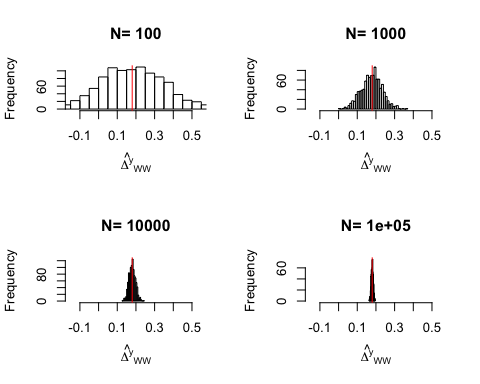
\includegraphics[width=0.5\linewidth]{STCI_files/figure-latex/montecarlohistbruteforcewwyB-1} }\subfloat[OLSX\label{fig:montecarlohistbruteforcewwyB2}]{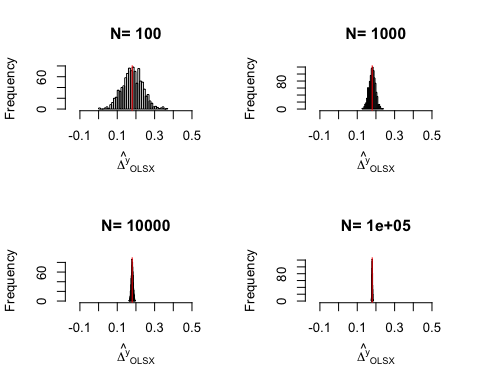
\includegraphics[width=0.5\linewidth]{STCI_files/figure-latex/montecarlohistbruteforcewwyB-2} }

}

\caption{Distribution of the $WW$ and $OLSX$ estimators in a Brute Force design over replications of samples of different sizes}\label{fig:montecarlohistbruteforcewwyB}
\end{figure}

Figure \ref{fig:montecarlohistbruteforcewwyB} shows that the gains in
precision from conditioning on \(y_i^B\) are spectacular in our
numerical example. They basically correspond to a gain in one order of
magnitude of sample size: the precision of the \(OLSX\) estimator
conditioning on \(y_i^B\) with a sample size of 100 is similar to the
precision of the \(OLS\) estimator not conditioning on \(y_i^B\) with a
sample size of \(1000\). This large gain in precision is largely due to
the fact that \(y_i\) and \(y_i^B\) are highly correlated. Not all
covariates perform so well in actual samples in the social sciences.

\BeginKnitrBlock{remark}
\iffalse{} {Remark. } \fi{}The ability to condition on covariates in
order to decrease sampling noise is a blessing but can also be a curse
when combined with significance testing. Indeed, you can now see that
you can run a lot of regressions (with and without some covariates,
interactions, etc) and maybe report only the statistically significant
ones. This is a bad practice that will lead to publication bias and
inflated treatment effects. Several possibilities in order to avoid
that:
\EndKnitrBlock{remark}

\begin{enumerate}
\def\labelenumi{\arabic{enumi}.}
\tightlist
\item
  Pre-register your analysis and explain which covariates you are going
  to use (with which interactions, etc) so that you cannot cherry pick
  your favorite results ex-post.
\item
  Use a stratified design for your RCT (more on this in Lecture 6) so
  that the important covariates are already balanced between treated and
  controls.
\item
  If unable to do all of the above, report results from regressions
  without controls and with various sets of controls. We do not expect
  the various treatment effect estimates to be the same (they cannot be,
  otherwise, they would have similar sampling noise), but we expect the
  following pattern: conditioning should systematically decrease
  sampling noise, not increase the treatment effect estimate. If
  conditioning on covariates makes a treatment effect significant, pay
  attention to why: is it because of a decrease in sampling noise
  (expected and OK) or because of an increase in treatment effect
  (beware specification search).
\end{enumerate}

\textbf{\textsc{Revise that especially in light of Chapter
\ref{sec:meta}}}

\BeginKnitrBlock{remark}
\iffalse{} {Remark. } \fi{}You might not be happy with the assumption of
linearity needed to use OLS to control for covariates. I have read
somewhere (forgot where) that this should not be much of a problem since
covariates are well balanced between groups by randomization, and thus a
linear first approximation to the function relating \(X_i\) to \(Y_i\)
should be fine. I tend not to buy that argument much. I have to run
simulations with a non linear relation between outcomes and controls and
see how linear OLS performs. If you do not like the linearity
assumption, you can always use any of the nonparametric observational
methods presented in Chapter \ref{sec:OM}.
\EndKnitrBlock{remark}

\subsubsection{Estimating Sampling
Noise}\label{estimating-sampling-noise}

In order to estimate sampling noise, you can either use the CLT-based
approach or resampling, either using the bootstrap or randomization
inference. In Section \ref{sec:estimsampnoise}, we have already
discussed how to estimate sampling noise when using the WW estimator
that we are using here. We are going to use the default and
heteroskedasticity-robust standard errors from OLS, which are both
CLT-based. Only the heteroskedasticity-robust standard errors are valid
under the assumptions that we have made so far. Homoskedasticity would
require constant treatment effects. Heteroskedasticity being small in
our numerical example, that should not matter much, but it could in
other applications.

\BeginKnitrBlock{example}
\protect\hypertarget{exm:unnamed-chunk-77}{}{\label{exm:unnamed-chunk-77}
}Let us first estimate sampling noise for the simple WW estimator
without control variables, using the OLS estimator.
\EndKnitrBlock{example}

\begin{Shaded}
\begin{Highlighting}[]
\NormalTok{sn.BF.simuls <-}\StringTok{ }\DecValTok{2}\OperatorTok{*}\KeywordTok{quantile}\NormalTok{(}\KeywordTok{abs}\NormalTok{(simuls.brute.force.ww[[}\StringTok{'1000'}\NormalTok{]][,}\StringTok{'WW'}\NormalTok{]}\OperatorTok{-}\KeywordTok{delta.y.ate}\NormalTok{(param)),}\DataTypeTok{probs=}\KeywordTok{c}\NormalTok{(}\FloatTok{0.99}\NormalTok{))}
\NormalTok{sn.BF.OLS.hetero <-}\StringTok{ }\DecValTok{2}\OperatorTok{*}\KeywordTok{qnorm}\NormalTok{((delta}\OperatorTok{+}\DecValTok{1}\NormalTok{)}\OperatorTok{/}\DecValTok{2}\NormalTok{)}\OperatorTok{*}\KeywordTok{sqrt}\NormalTok{(}\KeywordTok{vcovHC}\NormalTok{(reg.y.R.ols,}\DataTypeTok{type=}\StringTok{'HC2'}\NormalTok{)[}\DecValTok{2}\NormalTok{,}\DecValTok{2}\NormalTok{])}
\NormalTok{sn.BF.OLS.homo <-}\StringTok{ }\DecValTok{2}\OperatorTok{*}\KeywordTok{qnorm}\NormalTok{((delta}\OperatorTok{+}\DecValTok{1}\NormalTok{)}\OperatorTok{/}\DecValTok{2}\NormalTok{)}\OperatorTok{*}\KeywordTok{sqrt}\NormalTok{(}\KeywordTok{vcov}\NormalTok{(reg.y.R.ols)[}\DecValTok{2}\NormalTok{,}\DecValTok{2}\NormalTok{])}
\end{Highlighting}
\end{Shaded}

The true value of the 99\% sampling noise with a sample size of 1000 and
no control variables is stemming from the simulations is 0.274. The 99\%
sampling noise estimated using heteroskedasticity robust OLS standard
errors is 0.295. The 99\% sampling noise estimated using default OLS
standard errors is 0.294.

Let us now estimate sampling noise for the simple WW estimator
conditioning on \(y_i^B\), using the OLS estimator.

\begin{Shaded}
\begin{Highlighting}[]
\NormalTok{sn.BF.simuls.yB <-}\StringTok{ }\DecValTok{2}\OperatorTok{*}\KeywordTok{quantile}\NormalTok{(}\KeywordTok{abs}\NormalTok{(simuls.brute.force.ww.yB[[}\StringTok{'1000'}\NormalTok{]][,}\StringTok{'WW'}\NormalTok{]}\OperatorTok{-}\KeywordTok{delta.y.ate}\NormalTok{(param)),}\DataTypeTok{probs=}\KeywordTok{c}\NormalTok{(}\FloatTok{0.99}\NormalTok{))}
\NormalTok{sn.BF.OLS.hetero.yB <-}\StringTok{ }\DecValTok{2}\OperatorTok{*}\KeywordTok{qnorm}\NormalTok{((delta}\OperatorTok{+}\DecValTok{1}\NormalTok{)}\OperatorTok{/}\DecValTok{2}\NormalTok{)}\OperatorTok{*}\KeywordTok{sqrt}\NormalTok{(}\KeywordTok{vcovHC}\NormalTok{(reg.y.R.ols.yB,}\DataTypeTok{type=}\StringTok{'HC2'}\NormalTok{)[}\DecValTok{2}\NormalTok{,}\DecValTok{2}\NormalTok{])}
\NormalTok{sn.BF.OLS.homo.yB <-}\StringTok{ }\DecValTok{2}\OperatorTok{*}\KeywordTok{qnorm}\NormalTok{((delta}\OperatorTok{+}\DecValTok{1}\NormalTok{)}\OperatorTok{/}\DecValTok{2}\NormalTok{)}\OperatorTok{*}\KeywordTok{sqrt}\NormalTok{(}\KeywordTok{vcov}\NormalTok{(reg.y.R.ols.yB)[}\DecValTok{2}\NormalTok{,}\DecValTok{2}\NormalTok{])}
\end{Highlighting}
\end{Shaded}

The true value of the 99\% sampling noise with a sample size of 1000 and
no control variables is stemming from the simulations is 0.088. The 99\%
sampling noise estimated using heteroskedasticity robust OLS standard
errors is 0.092. The 99\% sampling noise estimated using default OLS
standard errors is 0.091.

Let's see how all of this works on average. Figure
\ref{fig:sampnoisewwBFCLTplot} shows that overall the sampling nois eis
much lower with \(OLSX\) than with \(WW\), as expected from Figure
\ref{fig:montecarlohistbruteforcewwyB}. The CLT-based estimator of
sampling noise accounting for heteroskedasticity (in blue) recovers true
sampling noise (in red) pretty well. Figure
\ref{fig:sampnoisewwBFCLTall} shows that the CLT-based estimates of
sampling noise are on point, except for \(N=10000\), where the CLT
slightly overestimates true sampling noise. Figure
\ref{fig:confintervalCLTBF} shows what happens when conditioning on
\(Y^B\) in a selection of 40 samples. The reduction in samplong noise is
pretty drastic here.

\begin{Shaded}
\begin{Highlighting}[]
\ControlFlowTok{for}\NormalTok{ (k }\ControlFlowTok{in}\NormalTok{ (}\DecValTok{1}\OperatorTok{:}\KeywordTok{length}\NormalTok{(N.sample)))\{}
\NormalTok{  simuls.brute.force.ww[[k]]}\OperatorTok{$}\NormalTok{CLT.noise <-}\StringTok{ }\DecValTok{2}\OperatorTok{*}\KeywordTok{qnorm}\NormalTok{((delta}\OperatorTok{+}\DecValTok{1}\NormalTok{)}\OperatorTok{/}\DecValTok{2}\NormalTok{)}\OperatorTok{*}\NormalTok{simuls.brute.force.ww[[k]][,}\StringTok{'se'}\NormalTok{]}
\NormalTok{  simuls.brute.force.ww.yB[[k]]}\OperatorTok{$}\NormalTok{CLT.noise <-}\StringTok{ }\DecValTok{2}\OperatorTok{*}\KeywordTok{qnorm}\NormalTok{((delta}\OperatorTok{+}\DecValTok{1}\NormalTok{)}\OperatorTok{/}\DecValTok{2}\NormalTok{)}\OperatorTok{*}\NormalTok{simuls.brute.force.ww.yB[[k]][,}\StringTok{'se'}\NormalTok{]}
\NormalTok{\}}

\NormalTok{samp.noise.ww.BF <-}\StringTok{ }\KeywordTok{sapply}\NormalTok{(}\KeywordTok{lapply}\NormalTok{(simuls.brute.force.ww,}\StringTok{`}\DataTypeTok{[}\StringTok{`}\NormalTok{,,}\DecValTok{1}\NormalTok{),samp.noise,}\DataTypeTok{delta=}\NormalTok{delta)}
\NormalTok{precision.ww.BF <-}\StringTok{ }\KeywordTok{sapply}\NormalTok{(}\KeywordTok{lapply}\NormalTok{(simuls.brute.force.ww,}\StringTok{`}\DataTypeTok{[}\StringTok{`}\NormalTok{,,}\DecValTok{1}\NormalTok{),precision,}\DataTypeTok{delta=}\NormalTok{delta)}
\KeywordTok{names}\NormalTok{(precision.ww.BF) <-}\StringTok{ }\NormalTok{N.sample}
\NormalTok{signal.to.noise.ww.BF <-}\StringTok{ }\KeywordTok{sapply}\NormalTok{(}\KeywordTok{lapply}\NormalTok{(simuls.brute.force.ww,}\StringTok{`}\DataTypeTok{[}\StringTok{`}\NormalTok{,,}\DecValTok{1}\NormalTok{),signal.to.noise,}\DataTypeTok{delta=}\NormalTok{delta,}\DataTypeTok{param=}\NormalTok{param)}
\KeywordTok{names}\NormalTok{(signal.to.noise.ww.BF) <-}\StringTok{ }\NormalTok{N.sample}
\NormalTok{table.noise.BF <-}\StringTok{ }\KeywordTok{cbind}\NormalTok{(samp.noise.ww.BF,precision.ww.BF,signal.to.noise.ww.BF)}
\KeywordTok{colnames}\NormalTok{(table.noise.BF) <-}\StringTok{ }\KeywordTok{c}\NormalTok{(}\StringTok{'sampling.noise'}\NormalTok{, }\StringTok{'precision'}\NormalTok{, }\StringTok{'signal.to.noise'}\NormalTok{)}
\NormalTok{table.noise.BF <-}\StringTok{ }\KeywordTok{as.data.frame}\NormalTok{(table.noise.BF)}
\NormalTok{table.noise.BF}\OperatorTok{$}\NormalTok{N <-}\StringTok{ }\KeywordTok{as.numeric}\NormalTok{(N.sample)}
\NormalTok{table.noise.BF}\OperatorTok{$}\NormalTok{ATE <-}\StringTok{ }\KeywordTok{rep}\NormalTok{(}\KeywordTok{delta.y.ate}\NormalTok{(param),}\KeywordTok{nrow}\NormalTok{(table.noise.BF))}
\ControlFlowTok{for}\NormalTok{ (k }\ControlFlowTok{in}\NormalTok{ (}\DecValTok{1}\OperatorTok{:}\KeywordTok{length}\NormalTok{(N.sample)))\{}
\NormalTok{  table.noise.BF}\OperatorTok{$}\NormalTok{CLT.noise[k] <-}\StringTok{ }\KeywordTok{mean}\NormalTok{(simuls.brute.force.ww[[k]]}\OperatorTok{$}\NormalTok{CLT.noise)}
\NormalTok{\}}
\NormalTok{table.noise.BF}\OperatorTok{$}\NormalTok{Method <-}\StringTok{ }\KeywordTok{rep}\NormalTok{(}\StringTok{"WW"}\NormalTok{,}\KeywordTok{nrow}\NormalTok{(table.noise.BF))}

\NormalTok{samp.noise.ww.BF.yB <-}\StringTok{ }\KeywordTok{sapply}\NormalTok{(}\KeywordTok{lapply}\NormalTok{(simuls.brute.force.ww.yB,}\StringTok{`}\DataTypeTok{[}\StringTok{`}\NormalTok{,,}\DecValTok{1}\NormalTok{),samp.noise,}\DataTypeTok{delta=}\NormalTok{delta)}
\NormalTok{precision.ww.BF.yB <-}\StringTok{ }\KeywordTok{sapply}\NormalTok{(}\KeywordTok{lapply}\NormalTok{(simuls.brute.force.ww.yB,}\StringTok{`}\DataTypeTok{[}\StringTok{`}\NormalTok{,,}\DecValTok{1}\NormalTok{),precision,}\DataTypeTok{delta=}\NormalTok{delta)}
\KeywordTok{names}\NormalTok{(precision.ww.BF.yB) <-}\StringTok{ }\NormalTok{N.sample}
\NormalTok{signal.to.noise.ww.BF.yB <-}\StringTok{ }\KeywordTok{sapply}\NormalTok{(}\KeywordTok{lapply}\NormalTok{(simuls.brute.force.ww.yB,}\StringTok{`}\DataTypeTok{[}\StringTok{`}\NormalTok{,,}\DecValTok{1}\NormalTok{),signal.to.noise,}\DataTypeTok{delta=}\NormalTok{delta,}\DataTypeTok{param=}\NormalTok{param)}
\KeywordTok{names}\NormalTok{(signal.to.noise.ww.BF.yB) <-}\StringTok{ }\NormalTok{N.sample}
\NormalTok{table.noise.BF.yB <-}\StringTok{ }\KeywordTok{cbind}\NormalTok{(samp.noise.ww.BF.yB,precision.ww.BF.yB,signal.to.noise.ww.BF.yB)}
\KeywordTok{colnames}\NormalTok{(table.noise.BF.yB) <-}\StringTok{ }\KeywordTok{c}\NormalTok{(}\StringTok{'sampling.noise'}\NormalTok{, }\StringTok{'precision'}\NormalTok{, }\StringTok{'signal.to.noise'}\NormalTok{)}
\NormalTok{table.noise.BF.yB <-}\StringTok{ }\KeywordTok{as.data.frame}\NormalTok{(table.noise.BF.yB)}
\NormalTok{table.noise.BF.yB}\OperatorTok{$}\NormalTok{N <-}\StringTok{ }\KeywordTok{as.numeric}\NormalTok{(N.sample)}
\NormalTok{table.noise.BF.yB}\OperatorTok{$}\NormalTok{ATE <-}\StringTok{ }\KeywordTok{rep}\NormalTok{(}\KeywordTok{delta.y.ate}\NormalTok{(param),}\KeywordTok{nrow}\NormalTok{(table.noise.BF.yB))}
\ControlFlowTok{for}\NormalTok{ (k }\ControlFlowTok{in}\NormalTok{ (}\DecValTok{1}\OperatorTok{:}\KeywordTok{length}\NormalTok{(N.sample)))\{}
\NormalTok{  table.noise.BF.yB}\OperatorTok{$}\NormalTok{CLT.noise[k] <-}\StringTok{ }\KeywordTok{mean}\NormalTok{(simuls.brute.force.ww.yB[[k]]}\OperatorTok{$}\NormalTok{CLT.noise)}
\NormalTok{\}}
\NormalTok{table.noise.BF.yB}\OperatorTok{$}\NormalTok{Method <-}\StringTok{ }\KeywordTok{rep}\NormalTok{(}\StringTok{"OLSX"}\NormalTok{,}\KeywordTok{nrow}\NormalTok{(table.noise.BF))}

\NormalTok{table.noise.BF.tot <-}\StringTok{ }\KeywordTok{rbind}\NormalTok{(table.noise.BF,table.noise.BF.yB)}
\NormalTok{table.noise.BF.tot}\OperatorTok{$}\NormalTok{Method <-}\StringTok{ }\KeywordTok{factor}\NormalTok{(table.noise.BF.tot}\OperatorTok{$}\NormalTok{Method,}\DataTypeTok{levels=}\KeywordTok{c}\NormalTok{(}\StringTok{"WW"}\NormalTok{,}\StringTok{"OLSX"}\NormalTok{))}

\KeywordTok{ggplot}\NormalTok{(table.noise.BF.tot, }\KeywordTok{aes}\NormalTok{(}\DataTypeTok{x=}\KeywordTok{as.factor}\NormalTok{(N), }\DataTypeTok{y=}\NormalTok{ATE,}\DataTypeTok{fill=}\NormalTok{Method)) }\OperatorTok{+}
\StringTok{  }\KeywordTok{geom_bar}\NormalTok{(}\DataTypeTok{position=}\KeywordTok{position_dodge}\NormalTok{(), }\DataTypeTok{stat=}\StringTok{"identity"}\NormalTok{, }\DataTypeTok{colour=}\StringTok{'black'}\NormalTok{) }\OperatorTok{+}
\StringTok{  }\KeywordTok{geom_errorbar}\NormalTok{(}\KeywordTok{aes}\NormalTok{(}\DataTypeTok{ymin=}\NormalTok{ATE}\OperatorTok{-}\NormalTok{sampling.noise}\OperatorTok{/}\DecValTok{2}\NormalTok{, }\DataTypeTok{ymax=}\NormalTok{ATE}\OperatorTok{+}\NormalTok{sampling.noise}\OperatorTok{/}\DecValTok{2}\NormalTok{), }\DataTypeTok{width=}\NormalTok{.}\DecValTok{2}\NormalTok{,}\DataTypeTok{position=}\KeywordTok{position_dodge}\NormalTok{(.}\DecValTok{9}\NormalTok{),}\DataTypeTok{color=}\StringTok{'red'}\NormalTok{) }\OperatorTok{+}
\StringTok{  }\KeywordTok{geom_errorbar}\NormalTok{(}\KeywordTok{aes}\NormalTok{(}\DataTypeTok{ymin=}\NormalTok{ATE}\OperatorTok{-}\NormalTok{CLT.noise}\OperatorTok{/}\DecValTok{2}\NormalTok{, }\DataTypeTok{ymax=}\NormalTok{ATE}\OperatorTok{+}\NormalTok{CLT.noise}\OperatorTok{/}\DecValTok{2}\NormalTok{), }\DataTypeTok{width=}\NormalTok{.}\DecValTok{2}\NormalTok{,}\DataTypeTok{position=}\KeywordTok{position_dodge}\NormalTok{(.}\DecValTok{9}\NormalTok{),}\DataTypeTok{color=}\StringTok{'blue'}\NormalTok{) }\OperatorTok{+}
\StringTok{  }\KeywordTok{xlab}\NormalTok{(}\StringTok{"Sample Size"}\NormalTok{)}\OperatorTok{+}
\StringTok{  }\KeywordTok{theme_bw}\NormalTok{()}\OperatorTok{+}
\StringTok{  }\KeywordTok{theme}\NormalTok{(}\DataTypeTok{legend.position=}\KeywordTok{c}\NormalTok{(}\FloatTok{0.85}\NormalTok{,}\FloatTok{0.88}\NormalTok{))}
\end{Highlighting}
\end{Shaded}

\begin{figure}[htbp]

{\centering 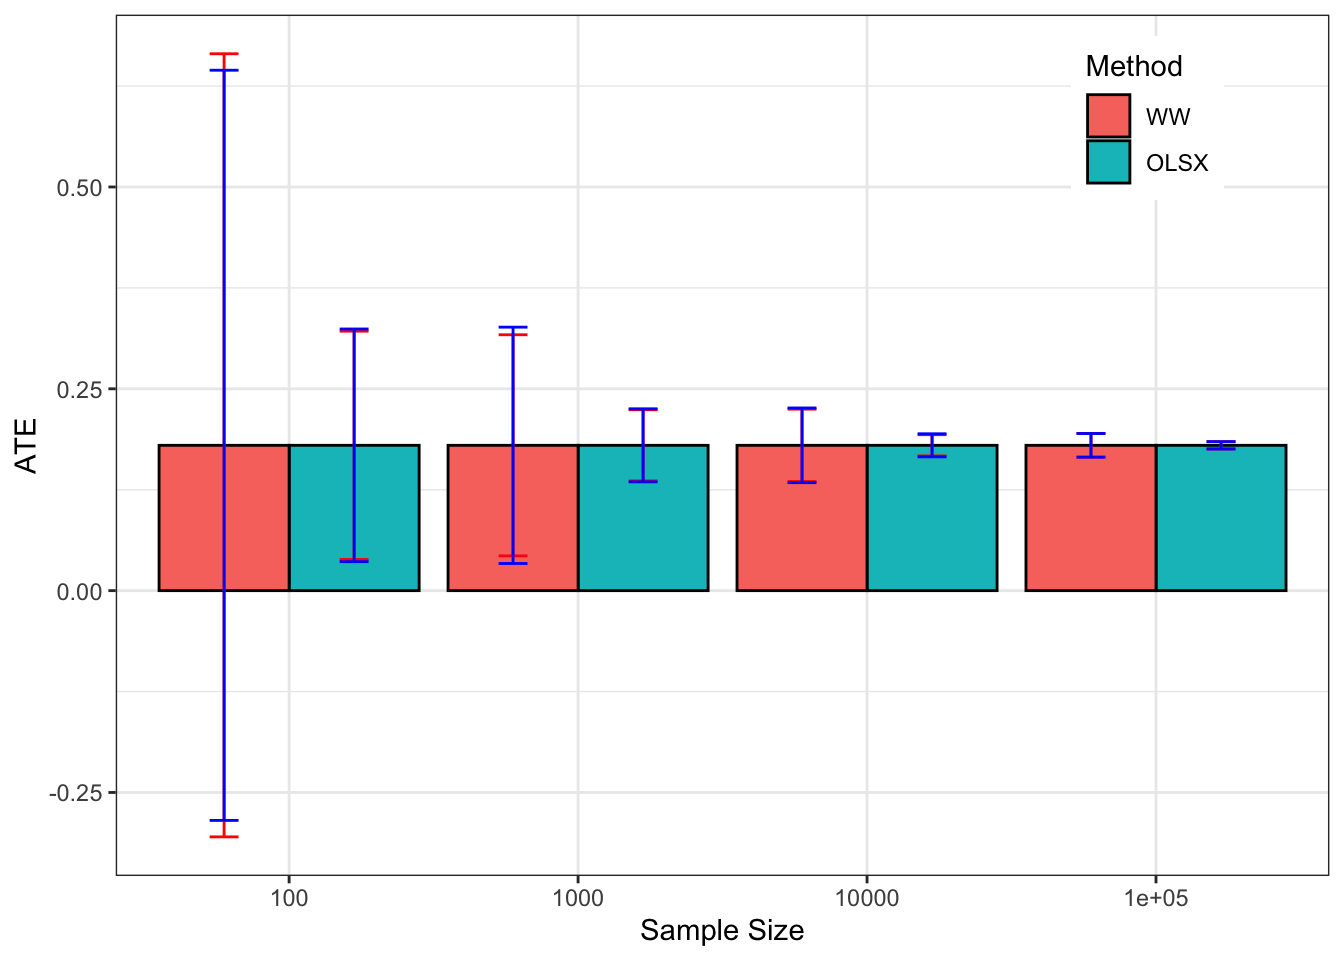
\includegraphics[width=0.5\linewidth]{STCI_files/figure-latex/sampnoisewwBFCLTplot-1} 

}

\caption{Average CLT-based approximations of sampling noise in the Brute Force design for $WW$ and $OLSX$ over replications of samples of different sizes (true sampling noise in red)}\label{fig:sampnoisewwBFCLTplot}
\end{figure}

\begin{Shaded}
\begin{Highlighting}[]
\KeywordTok{par}\NormalTok{(}\DataTypeTok{mfrow=}\KeywordTok{c}\NormalTok{(}\DecValTok{2}\NormalTok{,}\DecValTok{2}\NormalTok{))}
\ControlFlowTok{for}\NormalTok{ (i }\ControlFlowTok{in} \DecValTok{1}\OperatorTok{:}\KeywordTok{length}\NormalTok{(simuls.brute.force.ww))\{}
  \KeywordTok{hist}\NormalTok{(simuls.brute.force.ww[[i]][,}\StringTok{'CLT.noise'}\NormalTok{],}\DataTypeTok{main=}\KeywordTok{paste}\NormalTok{(}\StringTok{'N='}\NormalTok{,}\KeywordTok{as.character}\NormalTok{(N.sample[i])),}\DataTypeTok{xlab=}\KeywordTok{expression}\NormalTok{(}\KeywordTok{hat}\NormalTok{(}\DecValTok{2}\OperatorTok{*}\KeywordTok{bar}\NormalTok{(epsilon))[WW]),}\DataTypeTok{xlim=}\KeywordTok{c}\NormalTok{(}\KeywordTok{min}\NormalTok{(table.noise.BF[i,}\KeywordTok{colnames}\NormalTok{(table.noise)}\OperatorTok{==}\StringTok{'sampling.noise'}\NormalTok{],}\KeywordTok{min}\NormalTok{(simuls.brute.force.ww[[i]][,}\StringTok{'CLT.noise'}\NormalTok{])),}\KeywordTok{max}\NormalTok{(table.noise.BF[i,}\KeywordTok{colnames}\NormalTok{(table.noise)}\OperatorTok{==}\StringTok{'sampling.noise'}\NormalTok{],}\KeywordTok{max}\NormalTok{(simuls.brute.force.ww[[i]][,}\StringTok{'CLT.noise'}\NormalTok{]))))}
  \KeywordTok{abline}\NormalTok{(}\DataTypeTok{v=}\NormalTok{table.noise.BF[i,}\KeywordTok{colnames}\NormalTok{(table.noise)}\OperatorTok{==}\StringTok{'sampling.noise'}\NormalTok{],}\DataTypeTok{col=}\StringTok{"red"}\NormalTok{)}
\NormalTok{\}}
\KeywordTok{par}\NormalTok{(}\DataTypeTok{mfrow=}\KeywordTok{c}\NormalTok{(}\DecValTok{2}\NormalTok{,}\DecValTok{2}\NormalTok{))}
\ControlFlowTok{for}\NormalTok{ (i }\ControlFlowTok{in} \DecValTok{1}\OperatorTok{:}\KeywordTok{length}\NormalTok{(simuls.brute.force.ww.yB))\{}
  \KeywordTok{hist}\NormalTok{(simuls.brute.force.ww.yB[[i]][,}\StringTok{'CLT.noise'}\NormalTok{],}\DataTypeTok{main=}\KeywordTok{paste}\NormalTok{(}\StringTok{'N='}\NormalTok{,}\KeywordTok{as.character}\NormalTok{(N.sample[i])),}\DataTypeTok{xlab=}\KeywordTok{expression}\NormalTok{(}\KeywordTok{hat}\NormalTok{(}\DecValTok{2}\OperatorTok{*}\KeywordTok{bar}\NormalTok{(epsilon))[OLSX]),}\DataTypeTok{xlim=}\KeywordTok{c}\NormalTok{(}\KeywordTok{min}\NormalTok{(table.noise.BF.yB[i,}\KeywordTok{colnames}\NormalTok{(table.noise)}\OperatorTok{==}\StringTok{'sampling.noise'}\NormalTok{],}\KeywordTok{min}\NormalTok{(simuls.brute.force.ww.yB[[i]][,}\StringTok{'CLT.noise'}\NormalTok{])),}\KeywordTok{max}\NormalTok{(table.noise.BF.yB[i,}\KeywordTok{colnames}\NormalTok{(table.noise)}\OperatorTok{==}\StringTok{'sampling.noise'}\NormalTok{],}\KeywordTok{max}\NormalTok{(simuls.brute.force.ww.yB[[i]][,}\StringTok{'CLT.noise'}\NormalTok{]))))}
  \KeywordTok{abline}\NormalTok{(}\DataTypeTok{v=}\NormalTok{table.noise.BF.yB[i,}\KeywordTok{colnames}\NormalTok{(table.noise)}\OperatorTok{==}\StringTok{'sampling.noise'}\NormalTok{],}\DataTypeTok{col=}\StringTok{"red"}\NormalTok{)}
\NormalTok{\}}
\end{Highlighting}
\end{Shaded}

\begin{figure}[htbp]

{\centering \subfloat[$WW$\label{fig:sampnoisewwBFCLTall1}]{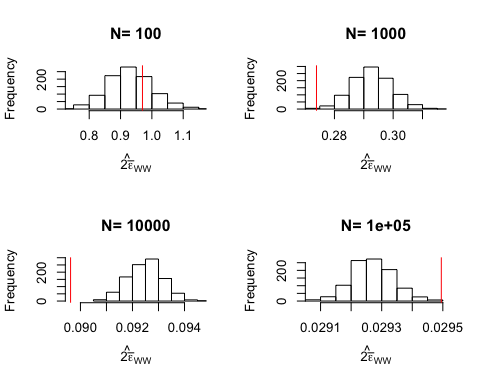
\includegraphics[width=0.5\linewidth]{STCI_files/figure-latex/sampnoisewwBFCLTall-1} }\subfloat[OLSX\label{fig:sampnoisewwBFCLTall2}]{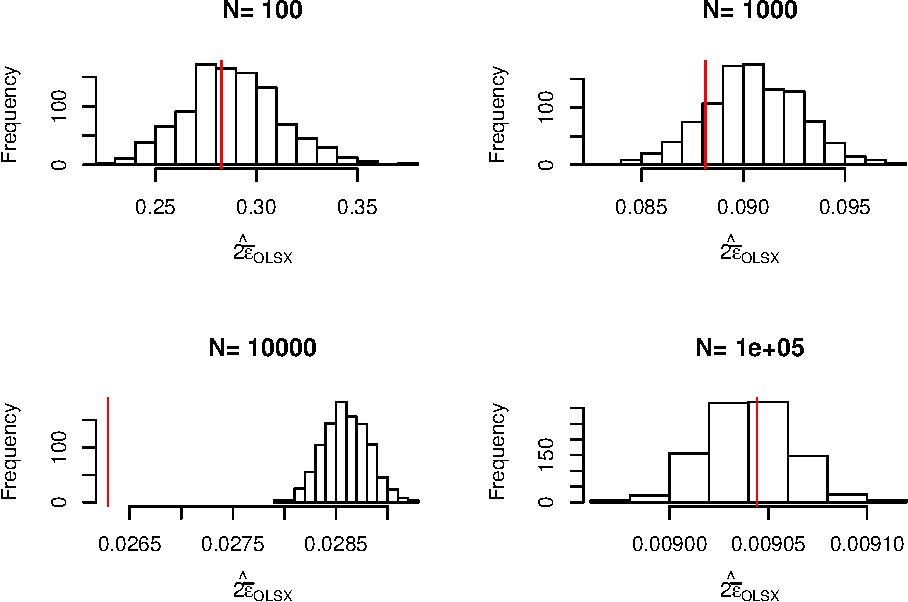
\includegraphics[width=0.5\linewidth]{STCI_files/figure-latex/sampnoisewwBFCLTall-2} }

}

\caption{Distribution of the CLT approximation of sampling noise in the Brute Force design for $WW$ and $OLSX$ over replications of samples of different sizes (true sampling noise in red)}\label{fig:sampnoisewwBFCLTall}
\end{figure}

\begin{Shaded}
\begin{Highlighting}[]
\NormalTok{N.plot <-}\StringTok{ }\DecValTok{40}
\NormalTok{plot.list <-}\StringTok{ }\KeywordTok{list}\NormalTok{()}
\NormalTok{limx <-}\StringTok{ }\KeywordTok{list}\NormalTok{(}\KeywordTok{c}\NormalTok{(}\OperatorTok{-}\FloatTok{0.65}\NormalTok{,}\FloatTok{1.25}\NormalTok{),}\KeywordTok{c}\NormalTok{(}\OperatorTok{-}\FloatTok{0.1}\NormalTok{,}\FloatTok{0.5}\NormalTok{),}\KeywordTok{c}\NormalTok{(}\DecValTok{0}\NormalTok{,}\FloatTok{0.30}\NormalTok{),}\KeywordTok{c}\NormalTok{(}\DecValTok{0}\NormalTok{,}\FloatTok{0.25}\NormalTok{))}

\ControlFlowTok{for}\NormalTok{ (k }\ControlFlowTok{in} \DecValTok{1}\OperatorTok{:}\KeywordTok{length}\NormalTok{(N.sample))\{}
  \KeywordTok{set.seed}\NormalTok{(}\DecValTok{1234}\NormalTok{)}
\NormalTok{  test.CLT.BF <-}\StringTok{ }\NormalTok{simuls.brute.force.ww[[k]][}\KeywordTok{sample}\NormalTok{(N.plot),}\KeywordTok{c}\NormalTok{(}\StringTok{'WW'}\NormalTok{,}\StringTok{'CLT.noise'}\NormalTok{)]}
\NormalTok{  test.CLT.BF <-}\StringTok{ }\KeywordTok{as.data.frame}\NormalTok{(}\KeywordTok{cbind}\NormalTok{(test.CLT.BF,}\KeywordTok{rep}\NormalTok{(}\KeywordTok{samp.noise}\NormalTok{(simuls.brute.force.ww[[k]][,}\StringTok{'WW'}\NormalTok{],}\DataTypeTok{delta=}\NormalTok{delta),N.plot)))}
  \KeywordTok{colnames}\NormalTok{(test.CLT.BF) <-}\StringTok{ }\KeywordTok{c}\NormalTok{(}\StringTok{'WW'}\NormalTok{,}\StringTok{'CLT.noise'}\NormalTok{,}\StringTok{'sampling.noise'}\NormalTok{)}
\NormalTok{  test.CLT.BF}\OperatorTok{$}\NormalTok{id <-}\StringTok{ }\DecValTok{1}\OperatorTok{:}\NormalTok{N.plot}
\NormalTok{  plot.test.CLT.BF <-}\StringTok{ }\KeywordTok{ggplot}\NormalTok{(test.CLT.BF, }\KeywordTok{aes}\NormalTok{(}\DataTypeTok{x=}\KeywordTok{as.factor}\NormalTok{(id), }\DataTypeTok{y=}\NormalTok{WW)) }\OperatorTok{+}
\StringTok{      }\KeywordTok{geom_bar}\NormalTok{(}\DataTypeTok{position=}\KeywordTok{position_dodge}\NormalTok{(), }\DataTypeTok{stat=}\StringTok{"identity"}\NormalTok{, }\DataTypeTok{colour=}\StringTok{'black'}\NormalTok{) }\OperatorTok{+}
\StringTok{      }\KeywordTok{geom_errorbar}\NormalTok{(}\KeywordTok{aes}\NormalTok{(}\DataTypeTok{ymin=}\NormalTok{WW}\OperatorTok{-}\NormalTok{sampling.noise}\OperatorTok{/}\DecValTok{2}\NormalTok{, }\DataTypeTok{ymax=}\NormalTok{WW}\OperatorTok{+}\NormalTok{sampling.noise}\OperatorTok{/}\DecValTok{2}\NormalTok{), }\DataTypeTok{width=}\NormalTok{.}\DecValTok{2}\NormalTok{,}\DataTypeTok{position=}\KeywordTok{position_dodge}\NormalTok{(.}\DecValTok{9}\NormalTok{),}\DataTypeTok{color=}\StringTok{'red'}\NormalTok{) }\OperatorTok{+}
\StringTok{      }\KeywordTok{geom_errorbar}\NormalTok{(}\KeywordTok{aes}\NormalTok{(}\DataTypeTok{ymin=}\NormalTok{WW}\OperatorTok{-}\NormalTok{CLT.noise}\OperatorTok{/}\DecValTok{2}\NormalTok{, }\DataTypeTok{ymax=}\NormalTok{WW}\OperatorTok{+}\NormalTok{CLT.noise}\OperatorTok{/}\DecValTok{2}\NormalTok{), }\DataTypeTok{width=}\NormalTok{.}\DecValTok{2}\NormalTok{,}\DataTypeTok{position=}\KeywordTok{position_dodge}\NormalTok{(.}\DecValTok{9}\NormalTok{),}\DataTypeTok{color=}\StringTok{'blue'}\NormalTok{) }\OperatorTok{+}
\StringTok{      }\KeywordTok{geom_hline}\NormalTok{(}\KeywordTok{aes}\NormalTok{(}\DataTypeTok{yintercept=}\KeywordTok{delta.y.ate}\NormalTok{(param)), }\DataTypeTok{colour=}\StringTok{"#990000"}\NormalTok{, }\DataTypeTok{linetype=}\StringTok{"dashed"}\NormalTok{)}\OperatorTok{+}
\StringTok{      }\KeywordTok{ylim}\NormalTok{(limx[[k]][}\DecValTok{1}\NormalTok{],limx[[k]][}\DecValTok{2}\NormalTok{])}\OperatorTok{+}
\StringTok{      }\KeywordTok{xlab}\NormalTok{(}\StringTok{"Sample id"}\NormalTok{)}\OperatorTok{+}
\StringTok{      }\KeywordTok{theme_bw}\NormalTok{()}\OperatorTok{+}
\StringTok{      }\KeywordTok{ggtitle}\NormalTok{(}\KeywordTok{paste}\NormalTok{(}\StringTok{"N="}\NormalTok{,N.sample[k]))}
\NormalTok{  plot.list[[k]] <-}\StringTok{ }\NormalTok{plot.test.CLT.BF}
\NormalTok{\}}
\NormalTok{plot.CI.BF <-}\StringTok{ }\KeywordTok{plot_grid}\NormalTok{(plot.list[[}\DecValTok{1}\NormalTok{]],plot.list[[}\DecValTok{2}\NormalTok{]],plot.list[[}\DecValTok{3}\NormalTok{]],plot.list[[}\DecValTok{4}\NormalTok{]],}\DataTypeTok{ncol=}\DecValTok{1}\NormalTok{,}\DataTypeTok{nrow=}\KeywordTok{length}\NormalTok{(N.sample))}
\KeywordTok{print}\NormalTok{(plot.CI.BF)}

\NormalTok{plot.list <-}\StringTok{ }\KeywordTok{list}\NormalTok{()}
\ControlFlowTok{for}\NormalTok{ (k }\ControlFlowTok{in} \DecValTok{1}\OperatorTok{:}\KeywordTok{length}\NormalTok{(N.sample))\{}
  \KeywordTok{set.seed}\NormalTok{(}\DecValTok{1234}\NormalTok{)}
\NormalTok{  test.CLT.BF.yB <-}\StringTok{ }\NormalTok{simuls.brute.force.ww.yB[[k]][}\KeywordTok{sample}\NormalTok{(N.plot),}\KeywordTok{c}\NormalTok{(}\StringTok{'WW'}\NormalTok{,}\StringTok{'CLT.noise'}\NormalTok{)]}
\NormalTok{  test.CLT.BF.yB <-}\StringTok{ }\KeywordTok{as.data.frame}\NormalTok{(}\KeywordTok{cbind}\NormalTok{(test.CLT.BF.yB,}\KeywordTok{rep}\NormalTok{(}\KeywordTok{samp.noise}\NormalTok{(simuls.brute.force.ww.yB[[k]][,}\StringTok{'WW'}\NormalTok{],}\DataTypeTok{delta=}\NormalTok{delta),N.plot)))}
  \KeywordTok{colnames}\NormalTok{(test.CLT.BF.yB) <-}\StringTok{ }\KeywordTok{c}\NormalTok{(}\StringTok{'WW'}\NormalTok{,}\StringTok{'CLT.noise'}\NormalTok{,}\StringTok{'sampling.noise'}\NormalTok{)}
\NormalTok{  test.CLT.BF.yB}\OperatorTok{$}\NormalTok{id <-}\StringTok{ }\DecValTok{1}\OperatorTok{:}\NormalTok{N.plot}
\NormalTok{  plot.test.CLT.BF.yB <-}\StringTok{ }\KeywordTok{ggplot}\NormalTok{(test.CLT.BF.yB, }\KeywordTok{aes}\NormalTok{(}\DataTypeTok{x=}\KeywordTok{as.factor}\NormalTok{(id), }\DataTypeTok{y=}\NormalTok{WW)) }\OperatorTok{+}
\StringTok{      }\KeywordTok{geom_bar}\NormalTok{(}\DataTypeTok{position=}\KeywordTok{position_dodge}\NormalTok{(), }\DataTypeTok{stat=}\StringTok{"identity"}\NormalTok{, }\DataTypeTok{colour=}\StringTok{'black'}\NormalTok{) }\OperatorTok{+}
\StringTok{      }\KeywordTok{geom_errorbar}\NormalTok{(}\KeywordTok{aes}\NormalTok{(}\DataTypeTok{ymin=}\NormalTok{WW}\OperatorTok{-}\NormalTok{sampling.noise}\OperatorTok{/}\DecValTok{2}\NormalTok{, }\DataTypeTok{ymax=}\NormalTok{WW}\OperatorTok{+}\NormalTok{sampling.noise}\OperatorTok{/}\DecValTok{2}\NormalTok{), }\DataTypeTok{width=}\NormalTok{.}\DecValTok{2}\NormalTok{,}\DataTypeTok{position=}\KeywordTok{position_dodge}\NormalTok{(.}\DecValTok{9}\NormalTok{),}\DataTypeTok{color=}\StringTok{'red'}\NormalTok{) }\OperatorTok{+}
\StringTok{      }\KeywordTok{geom_errorbar}\NormalTok{(}\KeywordTok{aes}\NormalTok{(}\DataTypeTok{ymin=}\NormalTok{WW}\OperatorTok{-}\NormalTok{CLT.noise}\OperatorTok{/}\DecValTok{2}\NormalTok{, }\DataTypeTok{ymax=}\NormalTok{WW}\OperatorTok{+}\NormalTok{CLT.noise}\OperatorTok{/}\DecValTok{2}\NormalTok{), }\DataTypeTok{width=}\NormalTok{.}\DecValTok{2}\NormalTok{,}\DataTypeTok{position=}\KeywordTok{position_dodge}\NormalTok{(.}\DecValTok{9}\NormalTok{),}\DataTypeTok{color=}\StringTok{'blue'}\NormalTok{) }\OperatorTok{+}
\StringTok{      }\KeywordTok{geom_hline}\NormalTok{(}\KeywordTok{aes}\NormalTok{(}\DataTypeTok{yintercept=}\KeywordTok{delta.y.ate}\NormalTok{(param)), }\DataTypeTok{colour=}\StringTok{"#990000"}\NormalTok{, }\DataTypeTok{linetype=}\StringTok{"dashed"}\NormalTok{)}\OperatorTok{+}
\StringTok{      }\KeywordTok{ylim}\NormalTok{(limx[[k]][}\DecValTok{1}\NormalTok{],limx[[k]][}\DecValTok{2}\NormalTok{])}\OperatorTok{+}
\StringTok{      }\KeywordTok{xlab}\NormalTok{(}\StringTok{"Sample id"}\NormalTok{)}\OperatorTok{+}
\StringTok{      }\KeywordTok{ylab}\NormalTok{(}\StringTok{"OLSX"}\NormalTok{)}\OperatorTok{+}
\StringTok{      }\KeywordTok{theme_bw}\NormalTok{()}\OperatorTok{+}
\StringTok{      }\KeywordTok{ggtitle}\NormalTok{(}\KeywordTok{paste}\NormalTok{(}\StringTok{"N="}\NormalTok{,N.sample[k]))}
\NormalTok{  plot.list[[k]] <-}\StringTok{ }\NormalTok{plot.test.CLT.BF.yB}
\NormalTok{\}}
\NormalTok{plot.CI.BF.yB <-}\StringTok{ }\KeywordTok{plot_grid}\NormalTok{(plot.list[[}\DecValTok{1}\NormalTok{]],plot.list[[}\DecValTok{2}\NormalTok{]],plot.list[[}\DecValTok{3}\NormalTok{]],plot.list[[}\DecValTok{4}\NormalTok{]],}\DataTypeTok{ncol=}\DecValTok{1}\NormalTok{,}\DataTypeTok{nrow=}\KeywordTok{length}\NormalTok{(N.sample))}
\KeywordTok{print}\NormalTok{(plot.CI.BF.yB)}
\end{Highlighting}
\end{Shaded}

\begin{figure}[htbp]

{\centering \subfloat[$WW$\label{fig:confintervalCLTBF1}]{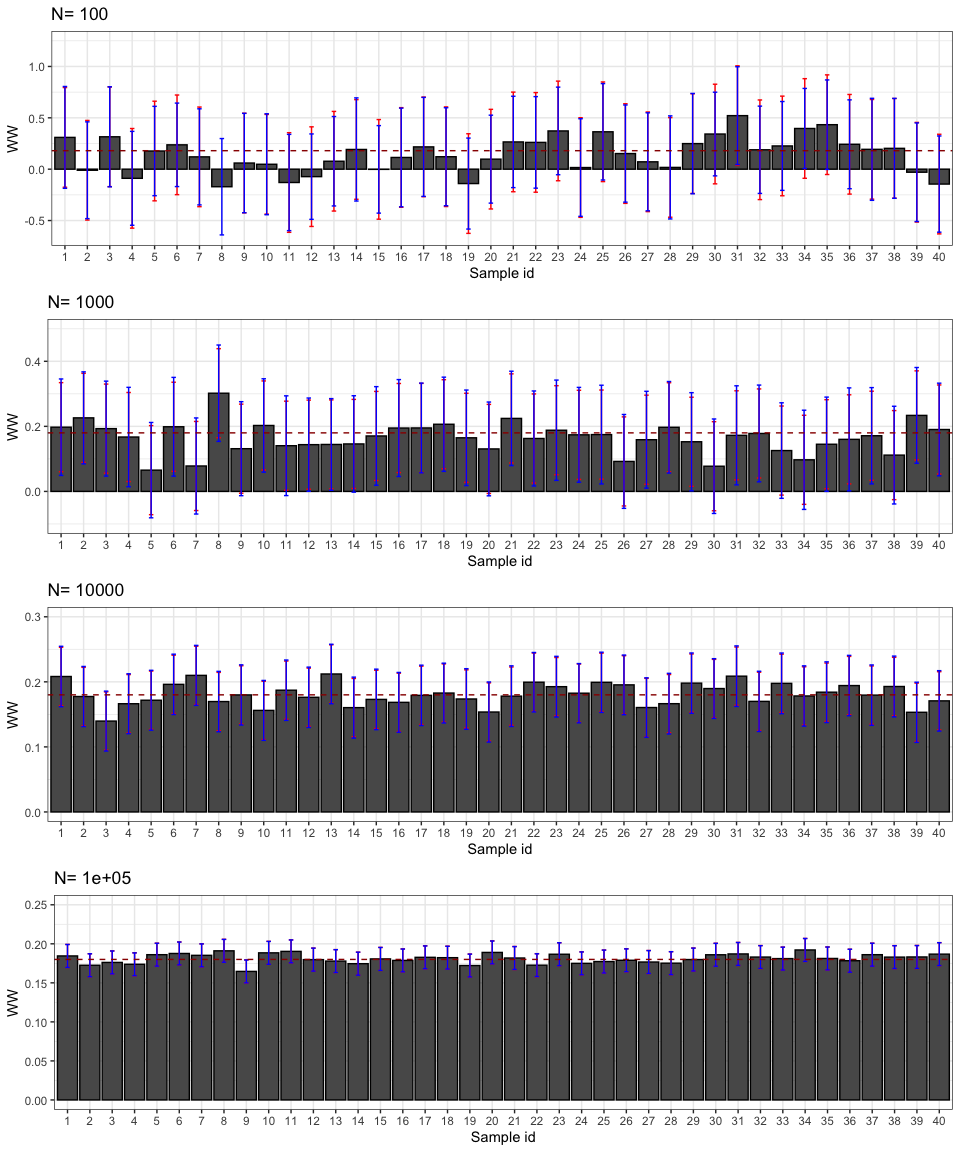
\includegraphics[width=0.5\linewidth]{STCI_files/figure-latex/confintervalCLTBF-1} }\subfloat[OLSX\label{fig:confintervalCLTBF2}]{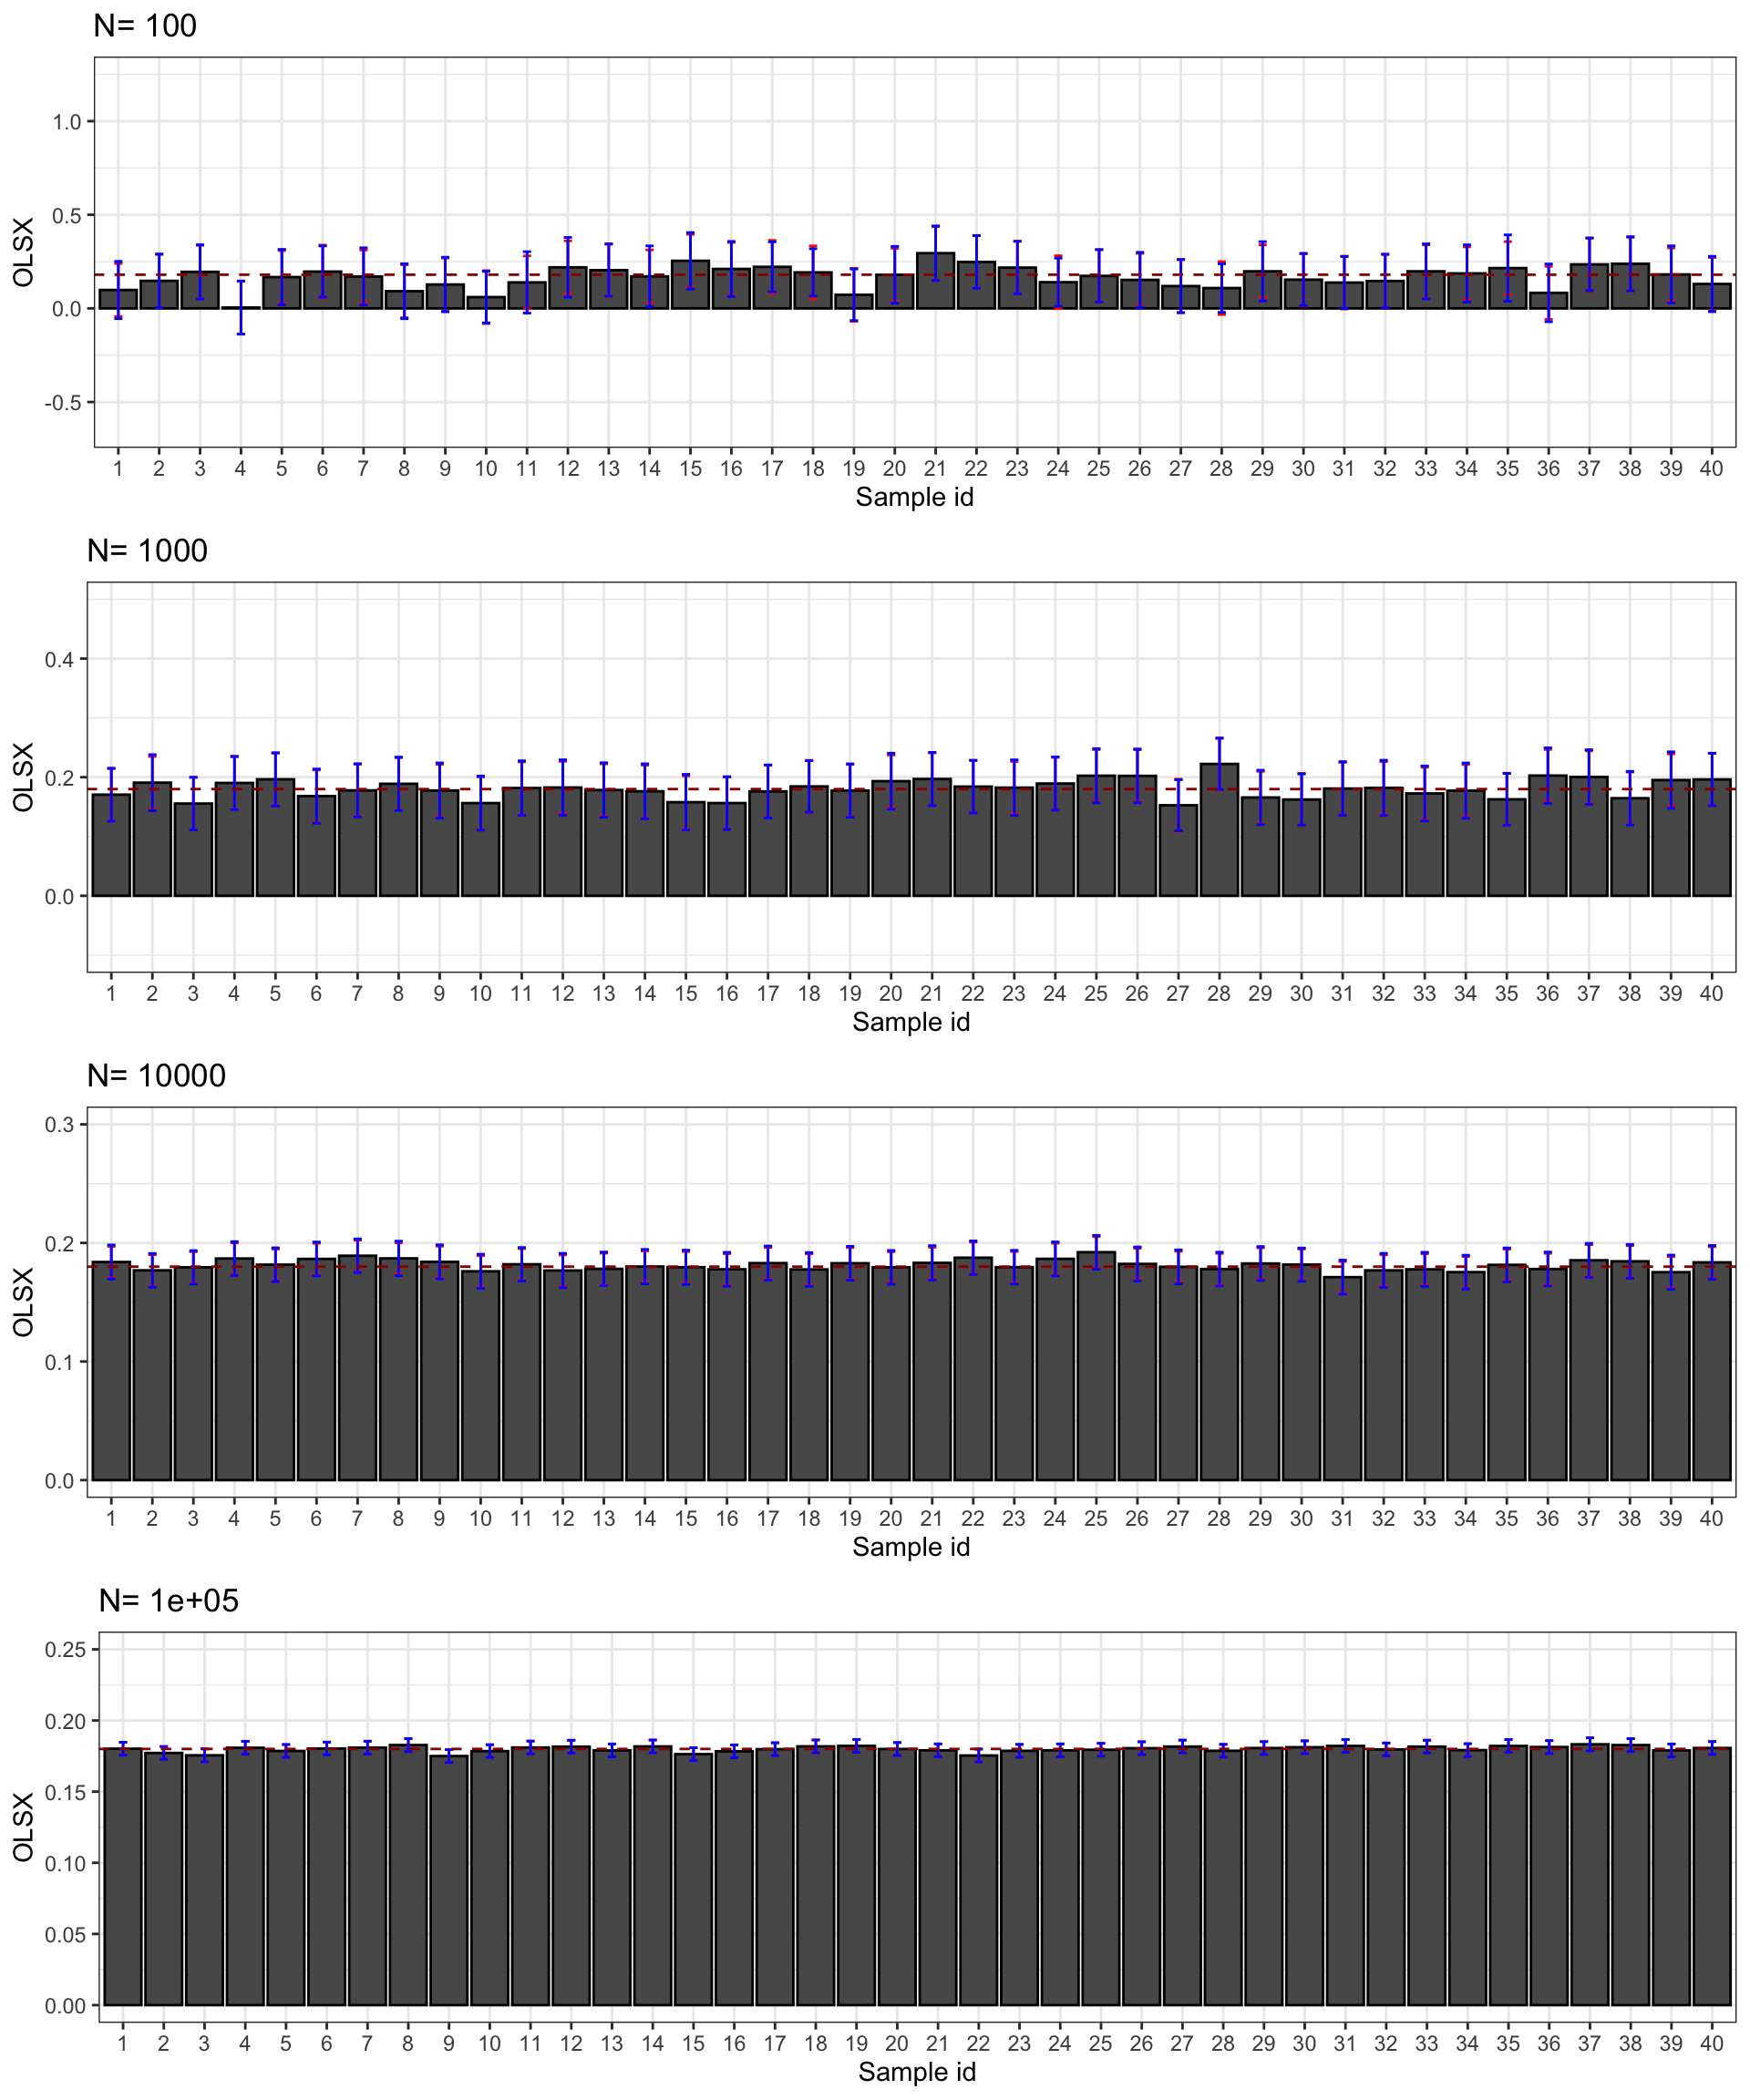
\includegraphics[width=0.5\linewidth]{STCI_files/figure-latex/confintervalCLTBF-2} }

}

\caption{CLT-based confidence intervals of $\hat{WW}$ and $\hat{OLSX}$ for $\delta=$ 0.99 over sample replications for various sample sizes (true confidence intervals in red)}\label{fig:confintervalCLTBF}
\end{figure}

\section{Randomization After Self-Selection}\label{sec:design2}

In Randomization After Self-Selection, individuals are randomly assigned
to the treatment after having expressed their willingness to receive it.
This design is able to recover the average effect of the Treatment on
the Treated (TT).

In order to explain this design clearly, and especially to make it clear
how it differs from the following one (randomization after eligibility),
I have to introduce a slightly more complex selection rule that we have
seen so far, one that includes self-selection, \textit{i.e.} take-up
decisions by agents. We are going to assume that there are two steps in
agents' participation process:

\begin{itemize}
\tightlist
\item
  Eligibility: agents' eligibility is assessed first, giving rise to a
  group of eligible individuals (\(E_i=1\)) and a group of non eligible
  individuals (\(E_i=0\)).
\item
  Self-selection: eligible agents can then decide whether they want to
  take-up the proposed treatment or not. \(D_i=1\) for those who do.
  \(D_i=0\) for those who do not. By convention, ineligibles have
  \(D_i=0\).
\end{itemize}

\BeginKnitrBlock{example}
\protect\hypertarget{exm:unnamed-chunk-78}{}{\label{exm:unnamed-chunk-78}
}In our numerical example, here are the equations operationalizing these
notions:
\EndKnitrBlock{example}

\begin{align*}
E_i & = \uns{y_i^B\leq\bar{y}} \\
D_i & = \uns{\underbrace{\bar{\alpha}+\theta\bar{\mu}-C_i}_{D_i^*}\geq0 \land E_i=1} \\
C_i & = \bar{c} + \gamma \mu_i + V_i\\
V_i & \sim \mathcal{N}(0,\sigma^2_V)
\end{align*}

Eligibility is still decided based on pre-treatment outcomes being
smaller than a threshold level \(\bar{y}\). Self-selection among
eligibles is decided by the net utility of the treatment \(D_i^*\) being
positive. Here, the net utility is composed of the average gain from the
treatment (assuming agents cannot foresee their idiosyncratic gain from
the treatment) \(\bar{\alpha}+\theta\bar{\mu}\) minus the cost of
participation \(C_i\). The cost of participation in turn depends on a
constant, on \(\mu_i\) and on a random shock orthogonal to everything
else \(V_i\). This cost might represent the administrative cost of
applying for the treatment and the opportunity cost of participating
into the treatment (foregone earnings and/or cost of time). Conditional
on eligiblity, self-selection is endogenous in this model since both the
gains and the cost of participation depend on \(\mu_i\). Costs depend on
\(\mu_i\) since most productive people may face lower administrative
costs but a higher opportunity cost of time.

Let's choose some values for the new parameters:

\begin{Shaded}
\begin{Highlighting}[]
\NormalTok{param <-}\StringTok{ }\KeywordTok{c}\NormalTok{(param,}\OperatorTok{-}\FloatTok{6.25}\NormalTok{,}\FloatTok{0.9}\NormalTok{,}\FloatTok{0.5}\NormalTok{)}
\KeywordTok{names}\NormalTok{(param) <-}\StringTok{ }\KeywordTok{c}\NormalTok{(}\StringTok{"barmu"}\NormalTok{,}\StringTok{"sigma2mu"}\NormalTok{,}\StringTok{"sigma2U"}\NormalTok{,}\StringTok{"barY"}\NormalTok{,}\StringTok{"rho"}\NormalTok{,}\StringTok{"theta"}\NormalTok{,}\StringTok{"sigma2epsilon"}\NormalTok{,}\StringTok{"sigma2eta"}\NormalTok{,}\StringTok{"delta"}\NormalTok{,}\StringTok{"baralpha"}\NormalTok{,}\StringTok{"barc"}\NormalTok{,}\StringTok{"gamma"}\NormalTok{,}\StringTok{"sigma2V"}\NormalTok{)}
\end{Highlighting}
\end{Shaded}

and let's generate a new dataset:

\begin{Shaded}
\begin{Highlighting}[]
\KeywordTok{set.seed}\NormalTok{(}\DecValTok{1234}\NormalTok{)}
\NormalTok{N <-}\DecValTok{1000}
\NormalTok{mu <-}\StringTok{ }\KeywordTok{rnorm}\NormalTok{(N,param[}\StringTok{"barmu"}\NormalTok{],}\KeywordTok{sqrt}\NormalTok{(param[}\StringTok{"sigma2mu"}\NormalTok{]))}
\NormalTok{UB <-}\StringTok{ }\KeywordTok{rnorm}\NormalTok{(N,}\DecValTok{0}\NormalTok{,}\KeywordTok{sqrt}\NormalTok{(param[}\StringTok{"sigma2U"}\NormalTok{]))}
\NormalTok{yB <-}\StringTok{ }\NormalTok{mu }\OperatorTok{+}\StringTok{ }\NormalTok{UB }
\NormalTok{YB <-}\StringTok{ }\KeywordTok{exp}\NormalTok{(yB)}
\NormalTok{E <-}\StringTok{ }\KeywordTok{ifelse}\NormalTok{(YB}\OperatorTok{<=}\NormalTok{param[}\StringTok{"barY"}\NormalTok{],}\DecValTok{1}\NormalTok{,}\DecValTok{0}\NormalTok{)}
\NormalTok{V <-}\StringTok{ }\KeywordTok{rnorm}\NormalTok{(N,}\DecValTok{0}\NormalTok{,param[}\StringTok{"sigma2V"}\NormalTok{])}
\NormalTok{Dstar <-}\StringTok{ }\NormalTok{param[}\StringTok{"baralpha"}\NormalTok{]}\OperatorTok{+}\NormalTok{param[}\StringTok{"theta"}\NormalTok{]}\OperatorTok{*}\NormalTok{param[}\StringTok{"barmu"}\NormalTok{]}\OperatorTok{-}\NormalTok{param[}\StringTok{"barc"}\NormalTok{]}\OperatorTok{-}\NormalTok{param[}\StringTok{"gamma"}\NormalTok{]}\OperatorTok{*}\NormalTok{mu}\OperatorTok{-}\NormalTok{V}
\NormalTok{Ds <-}\StringTok{ }\KeywordTok{ifelse}\NormalTok{(Dstar}\OperatorTok{>=}\DecValTok{0} \OperatorTok{&}\StringTok{ }\NormalTok{E}\OperatorTok{==}\DecValTok{1}\NormalTok{,}\DecValTok{1}\NormalTok{,}\DecValTok{0}\NormalTok{)}
\NormalTok{epsilon <-}\StringTok{ }\KeywordTok{rnorm}\NormalTok{(N,}\DecValTok{0}\NormalTok{,}\KeywordTok{sqrt}\NormalTok{(param[}\StringTok{"sigma2epsilon"}\NormalTok{]))}
\NormalTok{eta<-}\StringTok{ }\KeywordTok{rnorm}\NormalTok{(N,}\DecValTok{0}\NormalTok{,}\KeywordTok{sqrt}\NormalTok{(param[}\StringTok{"sigma2eta"}\NormalTok{]))}
\NormalTok{U0 <-}\StringTok{ }\NormalTok{param[}\StringTok{"rho"}\NormalTok{]}\OperatorTok{*}\NormalTok{UB }\OperatorTok{+}\StringTok{ }\NormalTok{epsilon}
\NormalTok{y0 <-}\StringTok{ }\NormalTok{mu }\OperatorTok{+}\StringTok{  }\NormalTok{U0 }\OperatorTok{+}\StringTok{ }\NormalTok{param[}\StringTok{"delta"}\NormalTok{]}
\NormalTok{alpha <-}\StringTok{ }\NormalTok{param[}\StringTok{"baralpha"}\NormalTok{]}\OperatorTok{+}\StringTok{  }\NormalTok{param[}\StringTok{"theta"}\NormalTok{]}\OperatorTok{*}\NormalTok{mu }\OperatorTok{+}\StringTok{ }\NormalTok{eta}
\NormalTok{y1 <-}\StringTok{ }\NormalTok{y0}\OperatorTok{+}\NormalTok{alpha}
\NormalTok{Y0 <-}\StringTok{ }\KeywordTok{exp}\NormalTok{(y0)}
\NormalTok{Y1 <-}\StringTok{ }\KeywordTok{exp}\NormalTok{(y1)}
\end{Highlighting}
\end{Shaded}

Let's compute the value of the TT parameter in this new model:

\begin{align*}
  \Delta^y_{TT} & = \bar{\alpha}+ \theta\esp{\mu_i|\mu_i+U_i^B\leq\bar{y} \land \bar{\alpha}+\theta\bar{\mu}-\bar{c}-\gamma\mu_i-V_i\geq0}
\end{align*}

To compute the expectation of a doubly censored normal, I use the
package \texttt{tmvtnorm}.

\begin{align*}
  (\mu_i,y_i^B,D_i^*) & = \mathcal{N}\left(\bar{\mu},\bar{\mu},\bar{\alpha}+(\theta-\gamma)\bar{\mu}-\bar{c},
                                        \left(\begin{array}{ccc}
                                              \sigma^2_{\mu} & \sigma^2_{\mu} & -\gamma\sigma^2_{\mu} \\
                                              \sigma^2_{\mu} & \sigma^2_{\mu} + \sigma^2_{U} & -\gamma\sigma^2_{\mu} \\
                                              -\gamma\sigma^2_{\mu} & -\gamma\sigma^2_{\mu} & \gamma^2\sigma^2_{\mu}+\sigma^2_{V}
                                              \end{array}
                                        \right)
                                      \right)
\end{align*}

\begin{Shaded}
\begin{Highlighting}[]
\NormalTok{mean.mu.yB.Dstar <-}\StringTok{ }\KeywordTok{c}\NormalTok{(param[}\StringTok{'barmu'}\NormalTok{],param[}\StringTok{'barmu'}\NormalTok{],param[}\StringTok{'baralpha'}\NormalTok{]}\OperatorTok{-}\StringTok{ }\NormalTok{param[}\StringTok{'barc'}\NormalTok{]}\OperatorTok{+}\NormalTok{(param[}\StringTok{'theta'}\NormalTok{]}\OperatorTok{-}\NormalTok{param[}\StringTok{'gamma'}\NormalTok{])}\OperatorTok{*}\NormalTok{param[}\StringTok{'barmu'}\NormalTok{])}
\NormalTok{cov.mu.yB.Dstar <-}\StringTok{ }\KeywordTok{matrix}\NormalTok{(}\KeywordTok{c}\NormalTok{(param[}\StringTok{'sigma2mu'}\NormalTok{],param[}\StringTok{"sigma2mu"}\NormalTok{],}\OperatorTok{-}\NormalTok{param[}\StringTok{'gamma'}\NormalTok{]}\OperatorTok{*}\NormalTok{param[}\StringTok{"sigma2mu"}\NormalTok{],}
\NormalTok{                            param[}\StringTok{"sigma2mu"}\NormalTok{],param[}\StringTok{'sigma2mu'}\NormalTok{]}\OperatorTok{+}\NormalTok{param[}\StringTok{'sigma2U'}\NormalTok{],}\OperatorTok{-}\NormalTok{param[}\StringTok{'gamma'}\NormalTok{]}\OperatorTok{*}\NormalTok{param[}\StringTok{"sigma2mu"}\NormalTok{],}
                            \OperatorTok{-}\NormalTok{param[}\StringTok{'gamma'}\NormalTok{]}\OperatorTok{*}\NormalTok{param[}\StringTok{"sigma2mu"}\NormalTok{],}\OperatorTok{-}\NormalTok{param[}\StringTok{'gamma'}\NormalTok{]}\OperatorTok{*}\NormalTok{param[}\StringTok{"sigma2mu"}\NormalTok{],param[}\StringTok{"sigma2mu"}\NormalTok{]}\OperatorTok{*}\NormalTok{(param[}\StringTok{'gamma'}\NormalTok{])}\OperatorTok{^}\DecValTok{2}\OperatorTok{+}\NormalTok{param[}\StringTok{'sigma2V'}\NormalTok{]),}\DecValTok{3}\NormalTok{,}\DecValTok{3}\NormalTok{,}\DataTypeTok{byrow=}\OtherTok{TRUE}\NormalTok{)}
\NormalTok{lower.cut <-}\StringTok{ }\KeywordTok{c}\NormalTok{(}\OperatorTok{-}\OtherTok{Inf}\NormalTok{,}\OperatorTok{-}\OtherTok{Inf}\NormalTok{,}\DecValTok{0}\NormalTok{)}
\NormalTok{upper.cut <-}\StringTok{ }\KeywordTok{c}\NormalTok{(}\OtherTok{Inf}\NormalTok{,}\KeywordTok{log}\NormalTok{(param[}\StringTok{'barY'}\NormalTok{]),}\OtherTok{Inf}\NormalTok{)}
\NormalTok{moments.cut <-}\StringTok{ }\KeywordTok{mtmvnorm}\NormalTok{(}\DataTypeTok{mean=}\NormalTok{mean.mu.yB.Dstar,}\DataTypeTok{sigma=}\NormalTok{cov.mu.yB.Dstar,}\DataTypeTok{lower=}\NormalTok{lower.cut,}\DataTypeTok{upper=}\NormalTok{upper.cut)}
\NormalTok{delta.y.tt <-}\StringTok{ }\NormalTok{param[}\StringTok{'baralpha'}\NormalTok{]}\OperatorTok{+}\StringTok{ }\NormalTok{param[}\StringTok{'theta'}\NormalTok{]}\OperatorTok{*}\NormalTok{moments.cut}\OperatorTok{$}\NormalTok{tmean[}\DecValTok{1}\NormalTok{]}
\NormalTok{delta.y.ww.self.select <-}\StringTok{ }\KeywordTok{mean}\NormalTok{(y[R}\OperatorTok{==}\DecValTok{1} \OperatorTok{&}\StringTok{ }\NormalTok{Ds}\OperatorTok{==}\DecValTok{1}\NormalTok{])}\OperatorTok{-}\KeywordTok{mean}\NormalTok{(y[R}\OperatorTok{==}\DecValTok{0} \OperatorTok{&}\StringTok{ }\NormalTok{Ds}\OperatorTok{==}\DecValTok{1}\NormalTok{])}
\end{Highlighting}
\end{Shaded}

The value of \(\Delta^y_{TT}\) in our illustration is now 0.17.

\subsection{Identification}\label{identification-1}

With Randomization After Self-Selection, identification requires two
assumptions:

\BeginKnitrBlock{definition}[Independence Among Self-Selected]
\protect\hypertarget{def:indepss}{}{\label{def:indepss}
\iffalse (Independence Among Self-Selected) \fi{} }We assume that the
randomized allocation of the program among applicants is well done:

\begin{align*}
  R_i\Ind(Y_i^0,Y_i^1)|D_i=1.
\end{align*}
\EndKnitrBlock{definition}

Independence can be enforced by the randomized allocation of the
treatment among the eligible applicants.

We need a second assumption:

\BeginKnitrBlock{definition}[Randomization After Self-Selection Validity]
\protect\hypertarget{def:rassval}{}{\label{def:rassval}
\iffalse (Randomization After Self-Selection Validity) \fi{} }We assume
that the randomized allocation of the program does not interfere with
how potential outcomes and self-selection are generated:

\begin{align*}
Y_i & = 
  \begin{cases}
    Y_i^1 & \text{ if } (R_i=1 \text{ and } D_i=1)   \\
    Y_i^0 & \text{ if } (R_i=0 \text{ and } D_i=1) \text{ or } D_i=0
  \end{cases}
\end{align*}
\EndKnitrBlock{definition}

with \(Y_i^1\), \(Y_i^0\) and \(D_i\) the same potential outcomes and
self-selection decisions as in a routine allocation of the treatment.

Under these assumptions, we have the following result:

\BeginKnitrBlock{theorem}[Identification With Randomization After Self-Selection]
\protect\hypertarget{thm:idrass}{}{\label{thm:idrass}
\iffalse (Identification With Randomization After Self-Selection) \fi{}
}Under Assumptions \ref{def:indepss} and \ref{def:rassval}, the WW
estimator among the self-selected identifies TT:

\begin{align*}
  \Delta^Y_{WW|D=1} & = \Delta^Y_{TT},
\end{align*}
\EndKnitrBlock{theorem}

with:

\begin{align*}
  \Delta^Y_{WW|D=1} & = \esp{Y_i|R_i=1,D_i=1} - \esp{Y_i|R_i=0,D_i=1}.
\end{align*}

\BeginKnitrBlock{proof}
\iffalse{} {Proof. } \fi{}

\begin{align*}
  \Delta^Y_{WW|D=1} & = \esp{Y_i|R_i=1,D_i=1} - \esp{Y_i|R_i=0,D_i=1} \\
                    & = \esp{Y^1_i|R_i=1,D_i=1} - \esp{Y^0_i|R_i=0,D_i=1} \\
                    & = \esp{Y_i^1|D_i=1}-\esp{Y_i^0|D_i=1}\\
                    & = \esp{Y_i^1-Y_i^0|D_i=1},
\end{align*}

where the second equality uses Randomization After Self-Selection
Validity, the third equality Independence Among Self-Selected and the
last equality the linearity of the expectation operator.
\EndKnitrBlock{proof}

\BeginKnitrBlock{remark}
\iffalse{} {Remark. } \fi{}The key intuitions for how Randomization
After Self-Selection solves the FPCI are:
\EndKnitrBlock{remark}

\begin{itemize}
\tightlist
\item
  By allowing for eligibilty and self-selection, we identify the agents
  that would benefit from the treatment in routine mode (the treated).
\item
  By randomly denying the treatment to some of the treated, we can
  estimate the counterfactual outcome of the treated by looking at the
  counterfactual outcome of the denied applicants:
  \(\esp{Y_i^0|D_i=1}=\esp{Y_i|R_i=0,D_i=1}\).
\end{itemize}

\BeginKnitrBlock{remark}
\iffalse{} {Remark. } \fi{}In practice, we use a pseudo-RNG to generate
a random allocation among applicants:
\EndKnitrBlock{remark}

\begin{align*}
  R_i^* & \sim \mathcal{U}[0,1]\\
  R_i & = 
  \begin{cases}
    1 & \text{ if } R_i^*\leq .5 \land D_i=1\\
    0 & \text{ if } R_i^*> .5 \land D_i=1
  \end{cases}
\end{align*}

\BeginKnitrBlock{example}
\protect\hypertarget{exm:unnamed-chunk-82}{}{\label{exm:unnamed-chunk-82}
}In our numerical example, the following R code generates two random
groups, one treated and one control, and imposes the Assumption of
Randomization After Self-Selection Validity:
\EndKnitrBlock{example}

\begin{Shaded}
\begin{Highlighting}[]
\CommentTok{#random allocation among self-selected}
\NormalTok{Rs <-}\StringTok{ }\KeywordTok{runif}\NormalTok{(N)}
\NormalTok{R <-}\StringTok{ }\KeywordTok{ifelse}\NormalTok{(Rs}\OperatorTok{<=}\NormalTok{.}\DecValTok{5} \OperatorTok{&}\StringTok{ }\NormalTok{Ds}\OperatorTok{==}\DecValTok{1}\NormalTok{,}\DecValTok{1}\NormalTok{,}\DecValTok{0}\NormalTok{)}
\NormalTok{y <-}\StringTok{ }\NormalTok{y1}\OperatorTok{*}\NormalTok{R}\OperatorTok{+}\NormalTok{y0}\OperatorTok{*}\NormalTok{(}\DecValTok{1}\OperatorTok{-}\NormalTok{R)}
\NormalTok{Y <-}\StringTok{ }\NormalTok{Y1}\OperatorTok{*}\NormalTok{R}\OperatorTok{+}\NormalTok{Y0}\OperatorTok{*}\NormalTok{(}\DecValTok{1}\OperatorTok{-}\NormalTok{R)}
\end{Highlighting}
\end{Shaded}

\subsection{Estimating TT}\label{estimating-tt}

\subsubsection{Using the WW Estimator}\label{using-the-ww-estimator-1}

As in the case of the Brute Force Design, we can use the WW estimator to
estimate the effect of the program with Randomization After
Self-Selection, except that this time the WW estimator is applied among
applicant to the program only:

\begin{align*}
  \hat{\Delta}^Y_{WW|D=1} & = \frac{1}{\sum_{i=1}^N D_iR_i}\sum_{i=1}^N Y_iD_iR_i-\frac{1}{\sum_{i=1}^N D_i(1-R_i)}\sum_{i=1}^N D_iY_i(1-R_i).
\end{align*}

\BeginKnitrBlock{example}
\protect\hypertarget{exm:unnamed-chunk-83}{}{\label{exm:unnamed-chunk-83}
}In our numerical example, we can form the WW estimator among
applicants:
\EndKnitrBlock{example}

\begin{Shaded}
\begin{Highlighting}[]
\NormalTok{delta.y.ww.self.select <-}\StringTok{ }\KeywordTok{mean}\NormalTok{(y[R}\OperatorTok{==}\DecValTok{1} \OperatorTok{&}\StringTok{ }\NormalTok{Ds}\OperatorTok{==}\DecValTok{1}\NormalTok{])}\OperatorTok{-}\KeywordTok{mean}\NormalTok{(y[R}\OperatorTok{==}\DecValTok{0} \OperatorTok{&}\StringTok{ }\NormalTok{Ds}\OperatorTok{==}\DecValTok{1}\NormalTok{])}
\end{Highlighting}
\end{Shaded}

WW among applicants is equal to 0.085. It is actually rather far from
the true value of 0.17, which reminds us that unbiasedness does not mean
that a given sample will not suffer from a large bias. We just drew a
bad sample where confounders are not very well balanced.

\subsubsection{Using OLS}\label{using-ols-1}

As in the Brute Force Design with the ATE, we can estimate the TT
parameter with Randomization After Self-Selection using the OLS
estimator. In the following regression run among applicants only (with
\(D_i=1\)), \(\beta\) estimates TT:

\begin{align*}
    Y_i &  = \alpha +  \beta R_i + U_i.
    \end{align*}

As a matter of fact, the OLS estimator without control variables is
numerically equivalent to the WW estimator.

\BeginKnitrBlock{example}
\protect\hypertarget{exm:unnamed-chunk-84}{}{\label{exm:unnamed-chunk-84}
}In our numerical example, here is the OLS regression:
\EndKnitrBlock{example}

\begin{Shaded}
\begin{Highlighting}[]
\NormalTok{reg.y.R.ols.self.select <-}\StringTok{ }\KeywordTok{lm}\NormalTok{(y[Ds}\OperatorTok{==}\DecValTok{1}\NormalTok{]}\OperatorTok{~}\NormalTok{R[Ds}\OperatorTok{==}\DecValTok{1}\NormalTok{])}
\end{Highlighting}
\end{Shaded}

The value of the OLS estimator is 0.085, which is identical to the WW
estimator among applicants.

\subsubsection{Using OLS Conditioning on
Covariates}\label{using-ols-conditioning-on-covariates-1}

We might want to condition on covariates in order to reduce the amount
of sampling noise. Parametrically, we can run the following OLS
regression among applicants (with \(D_i=1\)):

\begin{align*}
    Y_i &  = \alpha +  \beta R_i + \gamma' X_i + U_i.
\end{align*}

\(\beta\) estimates the TT.

\textbf{\textsc{Needed: proof. Especially check whether we need to
center covariates at the mean of the treatment group. I think so.}}

We can also use Matching to obtain a nonparametric estimator.

\BeginKnitrBlock{example}
\protect\hypertarget{exm:unnamed-chunk-85}{}{\label{exm:unnamed-chunk-85}
}Let us first compute the OLS estimator conditioning on \(y_i^B\):
\EndKnitrBlock{example}

\begin{Shaded}
\begin{Highlighting}[]
\NormalTok{reg.y.R.yB.ols.self.select <-}\StringTok{ }\KeywordTok{lm}\NormalTok{(y[Ds}\OperatorTok{==}\DecValTok{1}\NormalTok{] }\OperatorTok{~}\StringTok{ }\NormalTok{R[Ds}\OperatorTok{==}\DecValTok{1}\NormalTok{] }\OperatorTok{+}\StringTok{ }\NormalTok{yB[Ds}\OperatorTok{==}\DecValTok{1}\NormalTok{])}
\end{Highlighting}
\end{Shaded}

Our estimate of TT after conditioning on \(y_i^B\) is 0.145.
Conditioning on \(y_i^B\) has been able to solve part of the bias of the
WW problem estimator.

Let's now check whether conditioning on OLS has brought an improvement
in terms of decreased sampling noise.

\begin{Shaded}
\begin{Highlighting}[]
\NormalTok{monte.carlo.self.select.ww <-}\StringTok{ }\ControlFlowTok{function}\NormalTok{(s,N,param)\{}
  \KeywordTok{set.seed}\NormalTok{(s)}
\NormalTok{  mu <-}\StringTok{ }\KeywordTok{rnorm}\NormalTok{(N,param[}\StringTok{"barmu"}\NormalTok{],}\KeywordTok{sqrt}\NormalTok{(param[}\StringTok{"sigma2mu"}\NormalTok{]))}
\NormalTok{  UB <-}\StringTok{ }\KeywordTok{rnorm}\NormalTok{(N,}\DecValTok{0}\NormalTok{,}\KeywordTok{sqrt}\NormalTok{(param[}\StringTok{"sigma2U"}\NormalTok{]))}
\NormalTok{  yB <-}\StringTok{ }\NormalTok{mu }\OperatorTok{+}\StringTok{ }\NormalTok{UB }
\NormalTok{  YB <-}\StringTok{ }\KeywordTok{exp}\NormalTok{(yB)}
\NormalTok{  E <-}\StringTok{ }\KeywordTok{ifelse}\NormalTok{(YB}\OperatorTok{<=}\NormalTok{param[}\StringTok{"barY"}\NormalTok{],}\DecValTok{1}\NormalTok{,}\DecValTok{0}\NormalTok{)}
\NormalTok{  V <-}\StringTok{ }\KeywordTok{rnorm}\NormalTok{(N,}\DecValTok{0}\NormalTok{,param[}\StringTok{"sigma2V"}\NormalTok{])}
\NormalTok{  Dstar <-}\StringTok{ }\NormalTok{param[}\StringTok{"baralpha"}\NormalTok{]}\OperatorTok{+}\NormalTok{param[}\StringTok{"theta"}\NormalTok{]}\OperatorTok{*}\NormalTok{param[}\StringTok{"barmu"}\NormalTok{]}\OperatorTok{-}\NormalTok{param[}\StringTok{"barc"}\NormalTok{]}\OperatorTok{-}\NormalTok{param[}\StringTok{"gamma"}\NormalTok{]}\OperatorTok{*}\NormalTok{mu}\OperatorTok{-}\NormalTok{V}
\NormalTok{  Ds <-}\StringTok{ }\KeywordTok{ifelse}\NormalTok{(Dstar}\OperatorTok{>=}\DecValTok{0} \OperatorTok{&}\StringTok{ }\NormalTok{E}\OperatorTok{==}\DecValTok{1}\NormalTok{,}\DecValTok{1}\NormalTok{,}\DecValTok{0}\NormalTok{)}
\NormalTok{  epsilon <-}\StringTok{ }\KeywordTok{rnorm}\NormalTok{(N,}\DecValTok{0}\NormalTok{,}\KeywordTok{sqrt}\NormalTok{(param[}\StringTok{"sigma2epsilon"}\NormalTok{]))}
\NormalTok{  eta<-}\StringTok{ }\KeywordTok{rnorm}\NormalTok{(N,}\DecValTok{0}\NormalTok{,}\KeywordTok{sqrt}\NormalTok{(param[}\StringTok{"sigma2eta"}\NormalTok{]))}
\NormalTok{  U0 <-}\StringTok{ }\NormalTok{param[}\StringTok{"rho"}\NormalTok{]}\OperatorTok{*}\NormalTok{UB }\OperatorTok{+}\StringTok{ }\NormalTok{epsilon}
\NormalTok{  y0 <-}\StringTok{ }\NormalTok{mu }\OperatorTok{+}\StringTok{  }\NormalTok{U0 }\OperatorTok{+}\StringTok{ }\NormalTok{param[}\StringTok{"delta"}\NormalTok{]}
\NormalTok{  alpha <-}\StringTok{ }\NormalTok{param[}\StringTok{"baralpha"}\NormalTok{]}\OperatorTok{+}\StringTok{  }\NormalTok{param[}\StringTok{"theta"}\NormalTok{]}\OperatorTok{*}\NormalTok{mu }\OperatorTok{+}\StringTok{ }\NormalTok{eta}
\NormalTok{  y1 <-}\StringTok{ }\NormalTok{y0}\OperatorTok{+}\NormalTok{alpha}
\NormalTok{  Y0 <-}\StringTok{ }\KeywordTok{exp}\NormalTok{(y0)}
\NormalTok{  Y1 <-}\StringTok{ }\KeywordTok{exp}\NormalTok{(y1)}
  
  \CommentTok{#random allocation among self-selected}
\NormalTok{  Rs <-}\StringTok{ }\KeywordTok{runif}\NormalTok{(N)}
\NormalTok{  R <-}\StringTok{ }\KeywordTok{ifelse}\NormalTok{(Rs}\OperatorTok{<=}\NormalTok{.}\DecValTok{5} \OperatorTok{&}\StringTok{ }\NormalTok{Ds}\OperatorTok{==}\DecValTok{1}\NormalTok{,}\DecValTok{1}\NormalTok{,}\DecValTok{0}\NormalTok{)}
\NormalTok{  y <-}\StringTok{ }\NormalTok{y1}\OperatorTok{*}\NormalTok{R}\OperatorTok{+}\NormalTok{y0}\OperatorTok{*}\NormalTok{(}\DecValTok{1}\OperatorTok{-}\NormalTok{R)}
\NormalTok{  Y <-}\StringTok{ }\NormalTok{Y1}\OperatorTok{*}\NormalTok{R}\OperatorTok{+}\NormalTok{Y0}\OperatorTok{*}\NormalTok{(}\DecValTok{1}\OperatorTok{-}\NormalTok{R)}
  \KeywordTok{return}\NormalTok{(}\KeywordTok{mean}\NormalTok{(y[R}\OperatorTok{==}\DecValTok{1} \OperatorTok{&}\StringTok{ }\NormalTok{Ds}\OperatorTok{==}\DecValTok{1}\NormalTok{])}\OperatorTok{-}\KeywordTok{mean}\NormalTok{(y[R}\OperatorTok{==}\DecValTok{0} \OperatorTok{&}\StringTok{ }\NormalTok{Ds}\OperatorTok{==}\DecValTok{1}\NormalTok{]))}
\NormalTok{\}}

\NormalTok{simuls.self.select.ww.N <-}\StringTok{ }\ControlFlowTok{function}\NormalTok{(N,Nsim,param)\{}
\NormalTok{  simuls.self.select.ww <-}\StringTok{ }\KeywordTok{matrix}\NormalTok{(}\KeywordTok{unlist}\NormalTok{(}\KeywordTok{lapply}\NormalTok{(}\DecValTok{1}\OperatorTok{:}\NormalTok{Nsim,monte.carlo.self.select.ww,}\DataTypeTok{N=}\NormalTok{N,}\DataTypeTok{param=}\NormalTok{param)),}\DataTypeTok{nrow=}\NormalTok{Nsim,}\DataTypeTok{ncol=}\DecValTok{1}\NormalTok{,}\DataTypeTok{byrow=}\OtherTok{TRUE}\NormalTok{)}
  \KeywordTok{colnames}\NormalTok{(simuls.self.select.ww) <-}\StringTok{ }\KeywordTok{c}\NormalTok{(}\StringTok{'WW'}\NormalTok{)}
  \KeywordTok{return}\NormalTok{(simuls.self.select.ww)}
\NormalTok{\}}

\NormalTok{sf.simuls.self.select.ww.N <-}\StringTok{ }\ControlFlowTok{function}\NormalTok{(N,Nsim,param)\{}
  \KeywordTok{sfInit}\NormalTok{(}\DataTypeTok{parallel=}\OtherTok{TRUE}\NormalTok{,}\DataTypeTok{cpus=}\DecValTok{8}\NormalTok{)}
\NormalTok{  sim <-}\StringTok{ }\KeywordTok{matrix}\NormalTok{(}\KeywordTok{unlist}\NormalTok{(}\KeywordTok{sfLapply}\NormalTok{(}\DecValTok{1}\OperatorTok{:}\NormalTok{Nsim,monte.carlo.self.select.ww,}\DataTypeTok{N=}\NormalTok{N,}\DataTypeTok{param=}\NormalTok{param)),}\DataTypeTok{nrow=}\NormalTok{Nsim,}\DataTypeTok{ncol=}\DecValTok{1}\NormalTok{,}\DataTypeTok{byrow=}\OtherTok{TRUE}\NormalTok{)}
  \KeywordTok{sfStop}\NormalTok{()}
  \KeywordTok{colnames}\NormalTok{(sim) <-}\StringTok{ }\KeywordTok{c}\NormalTok{(}\StringTok{'WW'}\NormalTok{)}
  \KeywordTok{return}\NormalTok{(sim)}
\NormalTok{\}}

\NormalTok{Nsim <-}\StringTok{ }\DecValTok{1000}
\CommentTok{#Nsim <- 10}
\NormalTok{N.sample <-}\StringTok{ }\KeywordTok{c}\NormalTok{(}\DecValTok{100}\NormalTok{,}\DecValTok{1000}\NormalTok{,}\DecValTok{10000}\NormalTok{,}\DecValTok{100000}\NormalTok{)}
\CommentTok{#N.sample <- c(100,1000,10000)}
\CommentTok{#N.sample <- c(100,1000)}
\CommentTok{#N.sample <- c(100)}

\NormalTok{simuls.self.select.ww <-}\StringTok{ }\KeywordTok{lapply}\NormalTok{(N.sample,sf.simuls.self.select.ww.N,}\DataTypeTok{Nsim=}\NormalTok{Nsim,}\DataTypeTok{param=}\NormalTok{param)}
\KeywordTok{names}\NormalTok{(simuls.self.select.ww) <-}\StringTok{ }\NormalTok{N.sample}
\end{Highlighting}
\end{Shaded}

\begin{Shaded}
\begin{Highlighting}[]
\NormalTok{monte.carlo.self.select.yB.ww <-}\StringTok{ }\ControlFlowTok{function}\NormalTok{(s,N,param)\{}
  \KeywordTok{set.seed}\NormalTok{(s)}
\NormalTok{  mu <-}\StringTok{ }\KeywordTok{rnorm}\NormalTok{(N,param[}\StringTok{"barmu"}\NormalTok{],}\KeywordTok{sqrt}\NormalTok{(param[}\StringTok{"sigma2mu"}\NormalTok{]))}
\NormalTok{  UB <-}\StringTok{ }\KeywordTok{rnorm}\NormalTok{(N,}\DecValTok{0}\NormalTok{,}\KeywordTok{sqrt}\NormalTok{(param[}\StringTok{"sigma2U"}\NormalTok{]))}
\NormalTok{  yB <-}\StringTok{ }\NormalTok{mu }\OperatorTok{+}\StringTok{ }\NormalTok{UB }
\NormalTok{  YB <-}\StringTok{ }\KeywordTok{exp}\NormalTok{(yB)}
\NormalTok{  E <-}\StringTok{ }\KeywordTok{ifelse}\NormalTok{(YB}\OperatorTok{<=}\NormalTok{param[}\StringTok{"barY"}\NormalTok{],}\DecValTok{1}\NormalTok{,}\DecValTok{0}\NormalTok{)}
\NormalTok{  V <-}\StringTok{ }\KeywordTok{rnorm}\NormalTok{(N,}\DecValTok{0}\NormalTok{,param[}\StringTok{"sigma2V"}\NormalTok{])}
\NormalTok{  Dstar <-}\StringTok{ }\NormalTok{param[}\StringTok{"baralpha"}\NormalTok{]}\OperatorTok{+}\NormalTok{param[}\StringTok{"theta"}\NormalTok{]}\OperatorTok{*}\NormalTok{param[}\StringTok{"barmu"}\NormalTok{]}\OperatorTok{-}\NormalTok{param[}\StringTok{"barc"}\NormalTok{]}\OperatorTok{-}\NormalTok{param[}\StringTok{"gamma"}\NormalTok{]}\OperatorTok{*}\NormalTok{mu}\OperatorTok{-}\NormalTok{V}
\NormalTok{  Ds <-}\StringTok{ }\KeywordTok{ifelse}\NormalTok{(Dstar}\OperatorTok{>=}\DecValTok{0} \OperatorTok{&}\StringTok{ }\NormalTok{E}\OperatorTok{==}\DecValTok{1}\NormalTok{,}\DecValTok{1}\NormalTok{,}\DecValTok{0}\NormalTok{)}
\NormalTok{  epsilon <-}\StringTok{ }\KeywordTok{rnorm}\NormalTok{(N,}\DecValTok{0}\NormalTok{,}\KeywordTok{sqrt}\NormalTok{(param[}\StringTok{"sigma2epsilon"}\NormalTok{]))}
\NormalTok{  eta<-}\StringTok{ }\KeywordTok{rnorm}\NormalTok{(N,}\DecValTok{0}\NormalTok{,}\KeywordTok{sqrt}\NormalTok{(param[}\StringTok{"sigma2eta"}\NormalTok{]))}
\NormalTok{  U0 <-}\StringTok{ }\NormalTok{param[}\StringTok{"rho"}\NormalTok{]}\OperatorTok{*}\NormalTok{UB }\OperatorTok{+}\StringTok{ }\NormalTok{epsilon}
\NormalTok{  y0 <-}\StringTok{ }\NormalTok{mu }\OperatorTok{+}\StringTok{  }\NormalTok{U0 }\OperatorTok{+}\StringTok{ }\NormalTok{param[}\StringTok{"delta"}\NormalTok{]}
\NormalTok{  alpha <-}\StringTok{ }\NormalTok{param[}\StringTok{"baralpha"}\NormalTok{]}\OperatorTok{+}\StringTok{  }\NormalTok{param[}\StringTok{"theta"}\NormalTok{]}\OperatorTok{*}\NormalTok{mu }\OperatorTok{+}\StringTok{ }\NormalTok{eta}
\NormalTok{  y1 <-}\StringTok{ }\NormalTok{y0}\OperatorTok{+}\NormalTok{alpha}
\NormalTok{  Y0 <-}\StringTok{ }\KeywordTok{exp}\NormalTok{(y0)}
\NormalTok{  Y1 <-}\StringTok{ }\KeywordTok{exp}\NormalTok{(y1)}
  
  \CommentTok{#random allocation among self-selected}
\NormalTok{  Rs <-}\StringTok{ }\KeywordTok{runif}\NormalTok{(N)}
\NormalTok{  R <-}\StringTok{ }\KeywordTok{ifelse}\NormalTok{(Rs}\OperatorTok{<=}\NormalTok{.}\DecValTok{5} \OperatorTok{&}\StringTok{ }\NormalTok{Ds}\OperatorTok{==}\DecValTok{1}\NormalTok{,}\DecValTok{1}\NormalTok{,}\DecValTok{0}\NormalTok{)}
\NormalTok{  y <-}\StringTok{ }\NormalTok{y1}\OperatorTok{*}\NormalTok{R}\OperatorTok{+}\NormalTok{y0}\OperatorTok{*}\NormalTok{(}\DecValTok{1}\OperatorTok{-}\NormalTok{R)}
\NormalTok{  Y <-}\StringTok{ }\NormalTok{Y1}\OperatorTok{*}\NormalTok{R}\OperatorTok{+}\NormalTok{Y0}\OperatorTok{*}\NormalTok{(}\DecValTok{1}\OperatorTok{-}\NormalTok{R)}
\NormalTok{  reg.y.R.yB.ols.self.select <-}\StringTok{ }\KeywordTok{lm}\NormalTok{(y[Ds}\OperatorTok{==}\DecValTok{1}\NormalTok{] }\OperatorTok{~}\StringTok{ }\NormalTok{R[Ds}\OperatorTok{==}\DecValTok{1}\NormalTok{] }\OperatorTok{+}\StringTok{ }\NormalTok{yB[Ds}\OperatorTok{==}\DecValTok{1}\NormalTok{])}
  \KeywordTok{return}\NormalTok{(reg.y.R.yB.ols.self.select}\OperatorTok{$}\NormalTok{coef[}\DecValTok{2}\NormalTok{])}
\NormalTok{\}}

\NormalTok{simuls.self.select.yB.ww.N <-}\StringTok{ }\ControlFlowTok{function}\NormalTok{(N,Nsim,param)\{}
\NormalTok{  simuls.self.select.yB.ww <-}\StringTok{ }\KeywordTok{matrix}\NormalTok{(}\KeywordTok{unlist}\NormalTok{(}\KeywordTok{lapply}\NormalTok{(}\DecValTok{1}\OperatorTok{:}\NormalTok{Nsim,monte.carlo.self.select.yB.ww,}\DataTypeTok{N=}\NormalTok{N,}\DataTypeTok{param=}\NormalTok{param)),}\DataTypeTok{nrow=}\NormalTok{Nsim,}\DataTypeTok{ncol=}\DecValTok{1}\NormalTok{,}\DataTypeTok{byrow=}\OtherTok{TRUE}\NormalTok{)}
  \KeywordTok{colnames}\NormalTok{(simuls.self.select.yB.ww) <-}\StringTok{ }\KeywordTok{c}\NormalTok{(}\StringTok{'WW'}\NormalTok{)}
  \KeywordTok{return}\NormalTok{(simuls.self.select.yB.ww)}
\NormalTok{\}}

\NormalTok{sf.simuls.self.select.yB.ww.N <-}\StringTok{ }\ControlFlowTok{function}\NormalTok{(N,Nsim,param)\{}
  \KeywordTok{sfInit}\NormalTok{(}\DataTypeTok{parallel=}\OtherTok{TRUE}\NormalTok{,}\DataTypeTok{cpus=}\DecValTok{8}\NormalTok{)}
\NormalTok{  sim <-}\StringTok{ }\KeywordTok{matrix}\NormalTok{(}\KeywordTok{unlist}\NormalTok{(}\KeywordTok{sfLapply}\NormalTok{(}\DecValTok{1}\OperatorTok{:}\NormalTok{Nsim,monte.carlo.self.select.yB.ww,}\DataTypeTok{N=}\NormalTok{N,}\DataTypeTok{param=}\NormalTok{param)),}\DataTypeTok{nrow=}\NormalTok{Nsim,}\DataTypeTok{ncol=}\DecValTok{1}\NormalTok{,}\DataTypeTok{byrow=}\OtherTok{TRUE}\NormalTok{)}
  \KeywordTok{sfStop}\NormalTok{()}
  \KeywordTok{colnames}\NormalTok{(sim) <-}\StringTok{ }\KeywordTok{c}\NormalTok{(}\StringTok{'WW'}\NormalTok{)}
  \KeywordTok{return}\NormalTok{(sim)}
\NormalTok{\}}

\NormalTok{Nsim <-}\StringTok{ }\DecValTok{1000}
\CommentTok{#Nsim <- 10}
\NormalTok{N.sample <-}\StringTok{ }\KeywordTok{c}\NormalTok{(}\DecValTok{100}\NormalTok{,}\DecValTok{1000}\NormalTok{,}\DecValTok{10000}\NormalTok{,}\DecValTok{100000}\NormalTok{)}
\CommentTok{#N.sample <- c(100,1000,10000)}
\CommentTok{#N.sample <- c(100,1000)}
\CommentTok{#N.sample <- c(100)}

\NormalTok{simuls.self.select.yB.ww <-}\StringTok{ }\KeywordTok{lapply}\NormalTok{(N.sample,sf.simuls.self.select.yB.ww.N,}\DataTypeTok{Nsim=}\NormalTok{Nsim,}\DataTypeTok{param=}\NormalTok{param)}
\KeywordTok{names}\NormalTok{(simuls.self.select.yB.ww) <-}\StringTok{ }\NormalTok{N.sample}
\end{Highlighting}
\end{Shaded}

\begin{Shaded}
\begin{Highlighting}[]
\KeywordTok{par}\NormalTok{(}\DataTypeTok{mfrow=}\KeywordTok{c}\NormalTok{(}\DecValTok{2}\NormalTok{,}\DecValTok{2}\NormalTok{))}
\ControlFlowTok{for}\NormalTok{ (i }\ControlFlowTok{in} \DecValTok{1}\OperatorTok{:}\KeywordTok{length}\NormalTok{(simuls.self.select.ww))\{}
  \KeywordTok{hist}\NormalTok{(simuls.self.select.ww[[i]][,}\StringTok{'WW'}\NormalTok{],}\DataTypeTok{breaks=}\DecValTok{30}\NormalTok{,}\DataTypeTok{main=}\KeywordTok{paste}\NormalTok{(}\StringTok{'N='}\NormalTok{,}\KeywordTok{as.character}\NormalTok{(N.sample[i])),}\DataTypeTok{xlab=}\KeywordTok{expression}\NormalTok{(}\KeywordTok{hat}\NormalTok{(Delta}\OperatorTok{^}\NormalTok{yWW)),}\DataTypeTok{xlim=}\KeywordTok{c}\NormalTok{(}\OperatorTok{-}\FloatTok{0.15}\NormalTok{,}\FloatTok{0.55}\NormalTok{))}
  \KeywordTok{abline}\NormalTok{(}\DataTypeTok{v=}\NormalTok{delta.y.tt,}\DataTypeTok{col=}\StringTok{"red"}\NormalTok{)}
\NormalTok{\}}
\KeywordTok{par}\NormalTok{(}\DataTypeTok{mfrow=}\KeywordTok{c}\NormalTok{(}\DecValTok{2}\NormalTok{,}\DecValTok{2}\NormalTok{))}
\ControlFlowTok{for}\NormalTok{ (i }\ControlFlowTok{in} \DecValTok{1}\OperatorTok{:}\KeywordTok{length}\NormalTok{(simuls.self.select.yB.ww))\{}
  \KeywordTok{hist}\NormalTok{(simuls.self.select.yB.ww[[i]][,}\StringTok{'WW'}\NormalTok{],}\DataTypeTok{breaks=}\DecValTok{30}\NormalTok{,}\DataTypeTok{main=}\KeywordTok{paste}\NormalTok{(}\StringTok{'N='}\NormalTok{,}\KeywordTok{as.character}\NormalTok{(N.sample[i])),}\DataTypeTok{xlab=}\KeywordTok{expression}\NormalTok{(}\KeywordTok{hat}\NormalTok{(Delta}\OperatorTok{^}\NormalTok{yWW)),}\DataTypeTok{xlim=}\KeywordTok{c}\NormalTok{(}\OperatorTok{-}\FloatTok{0.15}\NormalTok{,}\FloatTok{0.55}\NormalTok{))}
  \KeywordTok{abline}\NormalTok{(}\DataTypeTok{v=}\NormalTok{delta.y.tt,}\DataTypeTok{col=}\StringTok{"red"}\NormalTok{)}
\NormalTok{\}}
\end{Highlighting}
\end{Shaded}

\begin{figure}[htbp]

{\centering \subfloat[$WW$\label{fig:montecarlohistselfselectww1}]{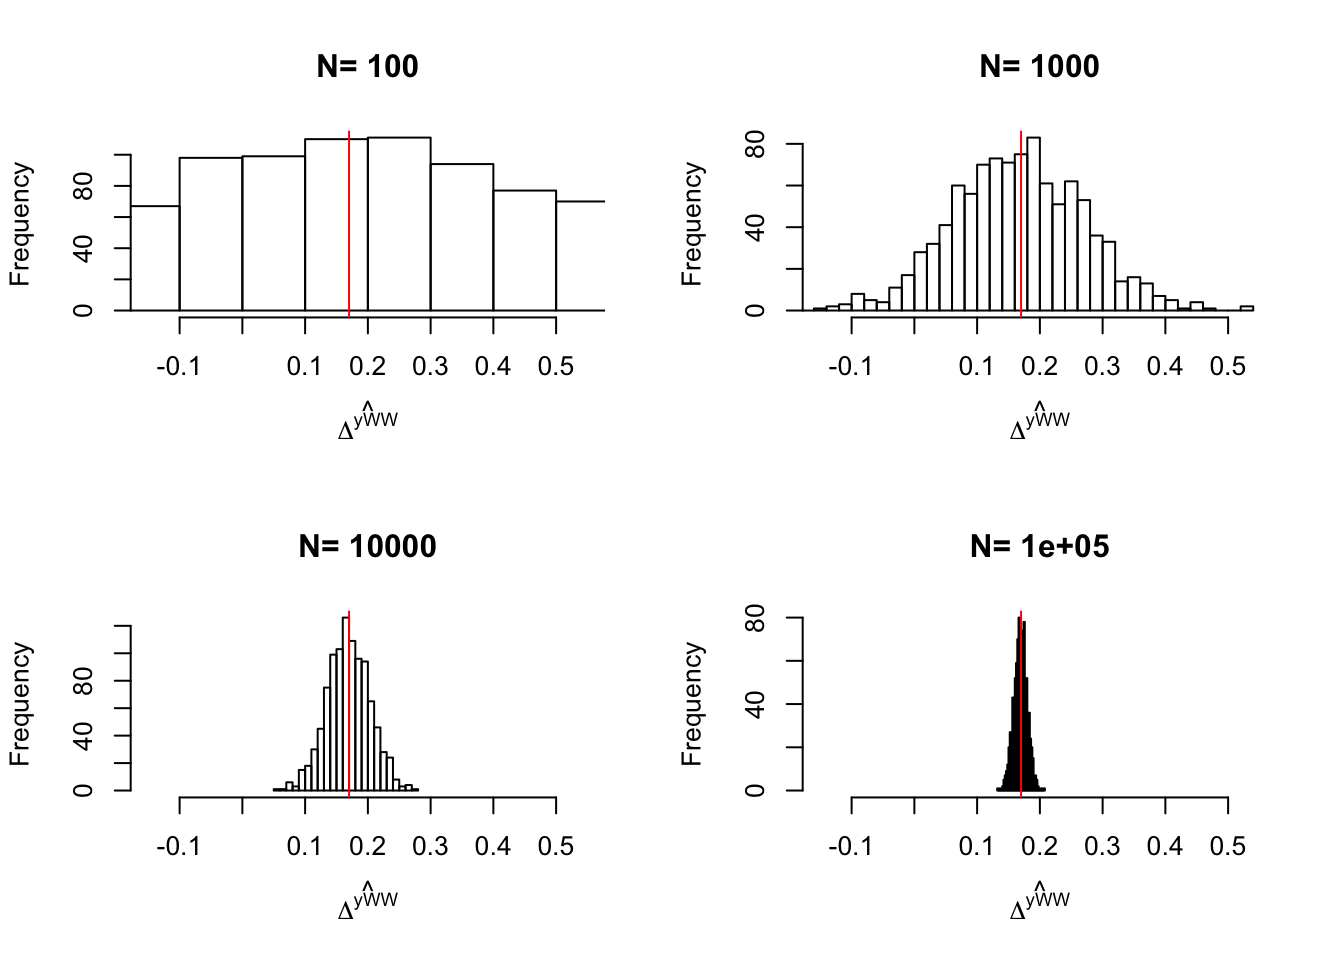
\includegraphics[width=0.5\linewidth]{STCI_files/figure-latex/montecarlohistselfselectww-1} }\subfloat[$OLSX$\label{fig:montecarlohistselfselectww2}]{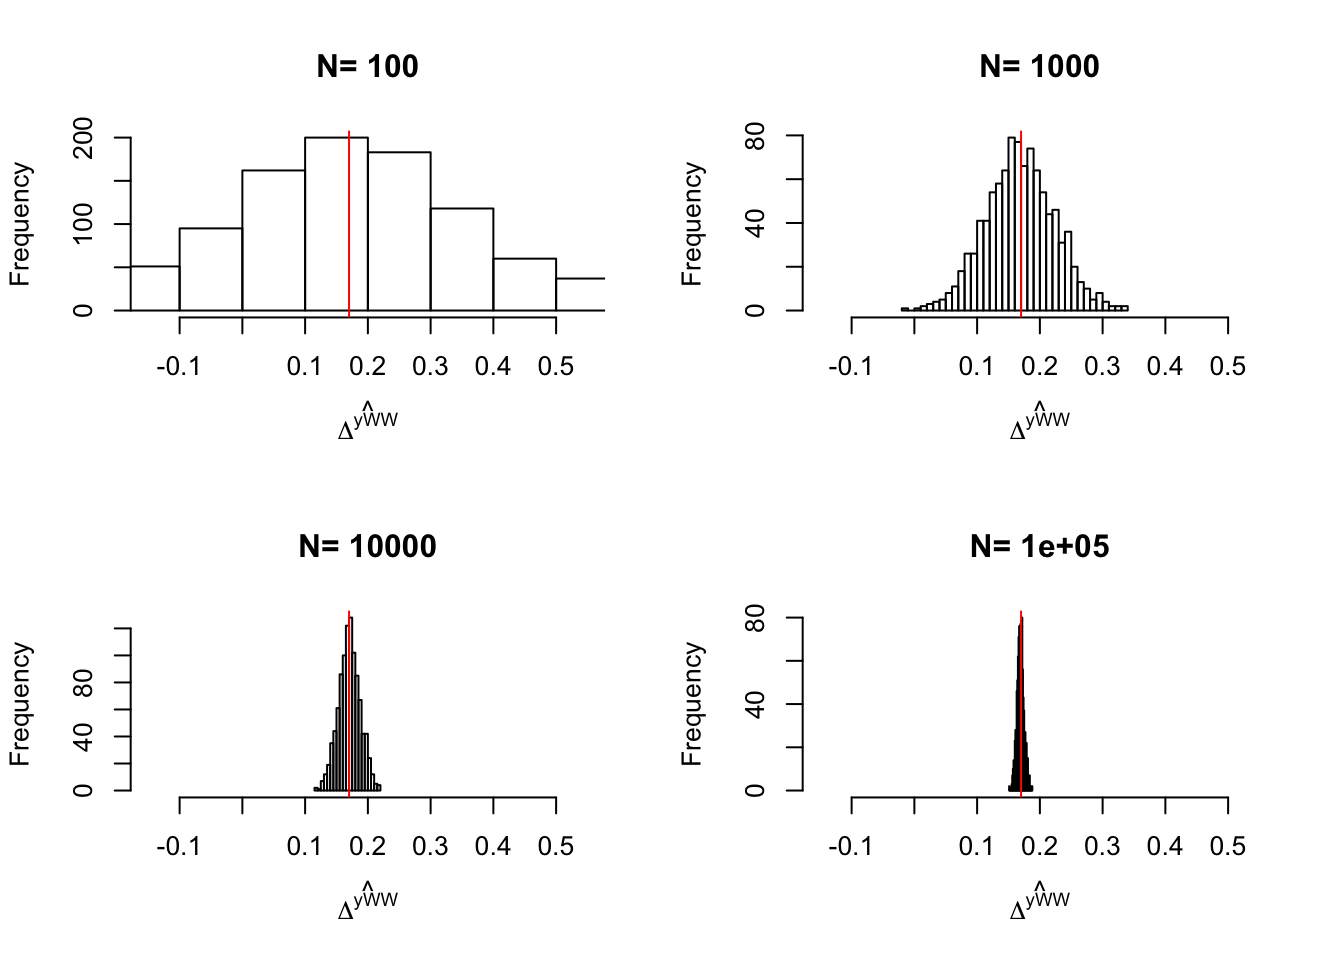
\includegraphics[width=0.5\linewidth]{STCI_files/figure-latex/montecarlohistselfselectww-2} }

}

\caption{Distribution of the $WW$ and $OLSX$ estimator with randomization after self-selection over replications of samples of different sizes}\label{fig:montecarlohistselfselectww}
\end{figure}

Figure \ref{fig:montecarlohistselfselectww} shows that, in our example,
conditioning on covariates improves precision by the same amount as an
increase in sample size by almost one order of magnitude.

\subsection{Estimating Sampling
Noise}\label{estimating-sampling-noise-1}

In order to estimate precision, we can either use the CLT, deriving
sampling noise from the heteroskedasticity-robust standard error OLS
estimates, or we can use some form of resampling as the bootstrap or
randomization inference.

\BeginKnitrBlock{example}
\protect\hypertarget{exm:unnamed-chunk-86}{}{\label{exm:unnamed-chunk-86}
}Let us derive the CLT-based estimates of sampling noise using the OLS
standard errors without conditioning on covariates first. I'm using the
sample size with \(N=1000\) as an example.
\EndKnitrBlock{example}

\begin{Shaded}
\begin{Highlighting}[]
\NormalTok{sn.RASS.simuls <-}\StringTok{ }\DecValTok{2}\OperatorTok{*}\KeywordTok{quantile}\NormalTok{(}\KeywordTok{abs}\NormalTok{(simuls.self.select.ww[[}\StringTok{'1000'}\NormalTok{]][,}\StringTok{'WW'}\NormalTok{]}\OperatorTok{-}\NormalTok{delta.y.tt),}\DataTypeTok{probs=}\KeywordTok{c}\NormalTok{(}\FloatTok{0.99}\NormalTok{))}
\NormalTok{sn.RASS.OLS.homo <-}\StringTok{ }\DecValTok{2}\OperatorTok{*}\KeywordTok{qnorm}\NormalTok{((.}\DecValTok{99}\OperatorTok{+}\DecValTok{1}\NormalTok{)}\OperatorTok{/}\DecValTok{2}\NormalTok{)}\OperatorTok{*}\KeywordTok{sqrt}\NormalTok{(}\KeywordTok{vcov}\NormalTok{(reg.y.R.ols.self.select)[}\DecValTok{2}\NormalTok{,}\DecValTok{2}\NormalTok{])}
\NormalTok{sn.RASS.OLS.hetero <-}\StringTok{ }\DecValTok{2}\OperatorTok{*}\KeywordTok{qnorm}\NormalTok{((.}\DecValTok{99}\OperatorTok{+}\DecValTok{1}\NormalTok{)}\OperatorTok{/}\DecValTok{2}\NormalTok{)}\OperatorTok{*}\KeywordTok{sqrt}\NormalTok{(}\KeywordTok{vcovHC}\NormalTok{(reg.y.R.ols.self.select,}\DataTypeTok{type=}\StringTok{'HC2'}\NormalTok{)[}\DecValTok{2}\NormalTok{,}\DecValTok{2}\NormalTok{])}
\end{Highlighting}
\end{Shaded}

True 99\% sampling noise (from the simulations) is 0.548. 99\% sampling
noise estimated using default OLS standard errors is 0.578. 99\%
sampling noise estimated using heteroskedasticity robust OLS standard
errors is 0.58.

Conditioning on covariates:

\begin{Shaded}
\begin{Highlighting}[]
\NormalTok{sn.RASS.simuls.yB <-}\StringTok{ }\DecValTok{2}\OperatorTok{*}\KeywordTok{quantile}\NormalTok{(}\KeywordTok{abs}\NormalTok{(simuls.self.select.yB.ww[[}\StringTok{'1000'}\NormalTok{]][,}\StringTok{'WW'}\NormalTok{]}\OperatorTok{-}\NormalTok{delta.y.tt),}\DataTypeTok{probs=}\KeywordTok{c}\NormalTok{(}\FloatTok{0.99}\NormalTok{))}
\NormalTok{sn.RASS.OLS.homo.yB <-}\StringTok{ }\DecValTok{2}\OperatorTok{*}\KeywordTok{qnorm}\NormalTok{((.}\DecValTok{99}\OperatorTok{+}\DecValTok{1}\NormalTok{)}\OperatorTok{/}\DecValTok{2}\NormalTok{)}\OperatorTok{*}\KeywordTok{sqrt}\NormalTok{(}\KeywordTok{vcov}\NormalTok{(reg.y.R.yB.ols.self.select)[}\DecValTok{2}\NormalTok{,}\DecValTok{2}\NormalTok{])}
\NormalTok{sn.RASS.OLS.hetero.yB <-}\StringTok{ }\DecValTok{2}\OperatorTok{*}\KeywordTok{qnorm}\NormalTok{((.}\DecValTok{99}\OperatorTok{+}\DecValTok{1}\NormalTok{)}\OperatorTok{/}\DecValTok{2}\NormalTok{)}\OperatorTok{*}\KeywordTok{sqrt}\NormalTok{(}\KeywordTok{vcovHC}\NormalTok{(reg.y.R.yB.ols.self.select,}\DataTypeTok{type=}\StringTok{'HC2'}\NormalTok{)[}\DecValTok{2}\NormalTok{,}\DecValTok{2}\NormalTok{])}
\end{Highlighting}
\end{Shaded}

True 99\% sampling noise (from the simulations) is 0.295. 99\% sampling
noise estimated using default OLS standard errors is 0.294. 99\%
sampling noise estimated using heteroskedasticity robust OLS standard
errors is 0.299.

\section{Randomization After Eligibility}\label{sec:design3}

In Randomization After Eligiblity, we randomly select two groups among
the eligibles. Members of the treated group are informed that they are
eligible to the program and are free to self-select into it. Members of
the control group are not enformed that they are eligible and cannot
enroll into the program. With Randomization After Eligiblity, we can
still recover the TT despite the fact that we have not randomized access
to the programs among the applicants. This is the magic of instrumental
variables. Let us detail the mechanics of this beautiful result.

\subsection{Identification}\label{identification-2}

In order to state the identification results in the Randomization After
Eligibility design rigorously, I need to define new potential outcomes:

\begin{itemize}
\tightlist
\item
  \(Y_i^{d,r}\) is the value of the outcome \(Y\) when individual \(i\)
  belongs to the program group \(d\) (\(d\in\left\{0,1\right\}\)) and
  has been randomized in group \(r\) (\(r\in\left\{0,1\right\}\)).
\item
  \(D_i^r\) is the value of the program participation decision when
  individual \(i\) has been assigned randomly to group \(r\).
\end{itemize}

\subsubsection{Identification of TT}\label{identification-of-tt}

In a Randomization After Eligiblity design, we need three assumptions to
ensure identification of the TT:

\BeginKnitrBlock{definition}[Independence Among Eligibles]
\protect\hypertarget{def:indelig}{}{\label{def:indelig}
\iffalse (Independence Among Eligibles) \fi{} }We assume that the
randomized allocation of the program among eligibles is well done:

\begin{align*}
  R_i\Ind(Y_i^{0,0},Y_i^{0,1},Y_i^{1,0},Y_i^{1,1},D_i^1,D_i^0)|E_i=1.
\end{align*}
\EndKnitrBlock{definition}

Independence can be enforced by the randomized allocation of information
about eligibility among the eligibles.

We need a second assumption:

\BeginKnitrBlock{definition}[Randomization After Eligibility Validity]
\protect\hypertarget{def:randeligvalid}{}{\label{def:randeligvalid}
\iffalse (Randomization After Eligibility Validity) \fi{} }We assume
that no eligibles that has been randomized out can take the treatment
and that the randomized allocation of the program does not interfere
with how potential outcomes and self-selection are generated:

\begin{align*}
D_i^0 & = 0\text{, } \forall i, \\
D_i & = D_i^1R_i+(1-R_i)D_i^0 \\
Y_i & = 
  \begin{cases}
    Y_i^{1,1} & \text{ if } (R_i=1 \text{ and } D_i=1)   \\
    Y_i^{0,1} & \text{ if } (R_i=1 \text{ and } D_i=0)    \\
    Y_i^{0,0} & \text{ if } R_i=0
  \end{cases}
\end{align*}
\EndKnitrBlock{definition} with \(Y_i^{1,1}\), \(Y_i^{0,1}\),
\(Y_i^{0,0}\), \(D_i^1\) and \(D^0_i\) the same potential outcomes and
self-selection decisions as in a routine allocation of the treatment.

We need a third assumption:

\BeginKnitrBlock{definition}[Exclusion Restriction of Eligibility]
\protect\hypertarget{def:exclrestric}{}{\label{def:exclrestric}
\iffalse (Exclusion Restriction of Eligibility) \fi{} }We assume that
there is no direct effect of being informed about eligibliity to the
program on outcomes:

\begin{align*}
  Y_i^{1,1} & = Y_i^{1,0}= Y_i^1\\
  Y_i^{0,1} & = Y_i^{0,0}= Y_i^0.
\end{align*}
\EndKnitrBlock{definition}

Under these assumptions, we have the following result:

\BeginKnitrBlock{theorem}[Identification of TT With Randomization After Eligibility]
\protect\hypertarget{thm:identTTRAE}{}{\label{thm:identTTRAE}
\iffalse (Identification of TT With Randomization After Eligibility)
\fi{} }Under Assumptions \ref{def:indelig}, \ref{def:randeligvalid} and
\ref{def:exclrestric}, the Bloom estimator among eligibles identifies
TT:

\begin{align*}
  \Delta^Y_{Bloom|E=1} & = \Delta^Y_{TT},
\end{align*}
\EndKnitrBlock{theorem} with:

\begin{align*}
  \Delta^Y_{Bloom|E=1} & = \frac{\Delta^Y_{WW|E=1}}{\Pr(D_i=1|R_i=1,E_i=1)} \\
  \Delta^Y_{WW|E=1} & =\esp{Y_i|R_i=1,E_i=1}-\esp{Y_i|R_i=0,E_i=1}.
\end{align*}

\BeginKnitrBlock{proof}
\iffalse{} {Proof. } \fi{}I keep the conditioning on \(E_i=1\) implicit
all along to save notation.

\begin{align*}
  \esp{Y_i|R_i=1} & = \esp{Y_i^{1,1}D_i+Y_i^{0,1}(1-D_i)|R_i=1} \\
                  & = \esp{Y_i^0+D_i(Y_i^1-Y_i^0)|R_i=1} \\
                  & = \esp{Y_i^0|R_i=1}+\esp{Y_i^1-Y_i^0|D_i=1,R_i=1}\Pr(D_i=1|R_i=1)\\
                  & = \esp{Y_i^0}+\esp{Y_i^1-Y_i^0|D_i=1}\Pr(D_i=1|R_i=1),
\end{align*}

where the first equality uses Assumption \ref{def:randeligvalid}, the
second equality Assumption \ref{def:exclrestric} and the last equality
Assumption \ref{def:indelig} and the fact that
\(D_i=1\Rightarrow R_i=1\). Using the same reasoning, we also have:

\begin{align*}
  \esp{Y_i|R_i=0} & = \esp{Y_i^{1,0}D_i+Y_i^{0,0}(1-D_i)|R_i=0} \\
                  & = \esp{Y_i^0|R_i=0} \\
                  & = \esp{Y_i^0}.
\end{align*}

A direct application of the formula for the Bloom estimator proves the
result.
\EndKnitrBlock{proof}

\subsubsection{Identification of ITE}\label{identification-of-ite}

The previous proof does not give a lot of intuition of how TT is
identified in the Randomization After Eligibility design. In order to
gain more insight, we are going to decompose the Bloom estimator, and
have a look at its numerator. The numerator of the Bloom estimator is a
With/Without comparison, and it identifies, under fairly light
conditions, another causal effect, the Intention to Treat Effect (ITE).

Let me first define the ITE:

\BeginKnitrBlock{definition}[Intention to Treat Effect]
\protect\hypertarget{def:ITE}{}{\label{def:ITE} \iffalse (Intention to Treat
Effect) \fi{} }In a Randomization After Eligibility design, the
Intention to Treat Effect (ITE) is the effect of receiving information
about eligiblity among eligibles:

\begin{align*}
  \Delta^Y_{ITE} & = \esp{Y_i^{D_i^1,1}-Y_i^{D_i^0,0}|E_i=1}.
\end{align*}
\EndKnitrBlock{definition}

Receiving information about eligibility has two impacts, in the general
framework that we have delineated so far: first, it triggers some
individuals into the treatment (those for which \(D_i^1\neq0\)); second,
it might have a direct effect on outcomes (\(Y_i^{d,1}\neq Y_i^{d,0}\)).
This second effect is the effect of annoucing eligiblity that does not
goes through participation into the program. For example, it is possible
that announcing eligibility to a retirement program makes me save more
for retirement, even if I end up not taking up the proposed program.

The two causal channels that are at work within the ITE can be seen more
clearly after some manipulations:

\begin{align}
  \Delta^Y_{ITE} & = \esp{Y_i^{1,1}D^1_i+Y_i^{0,1}(1-D_i^1)-(Y_i^{1,0}D^0_i+Y_i^{0,0}(1-D_i^0))|E_i=1}\nonumber \\
                & = \esp{Y_i^{1,1}D^1_i+Y_i^{0,1}(1-D_i^1)-(Y_i^{0,0}(D_i^1+1-D_i^1))|E_i=1}\nonumber \\
                & = \esp{(Y_i^{1,1}-Y_i^{0,0})D^1_i+(Y_i^{0,1}-Y_i^{0,0})(1-D_i^1)|E_i=1}\nonumber \\
                & = \esp{Y_i^{1,1}-Y_i^{0,0}|D^1_i=1,E_i=1}\Pr(D^1_i=1|E_i=1)\nonumber \\
                & \phantom{=}+\esp{Y_i^{0,1}-Y_i^{0,0}|D_i^1=0,E_i=1}\Pr(D_i^1=0|E_i=1),\label{eq:ITE2}
\end{align}

where the first equality follows from Assumption \ref{def:randeligvalid}
and the second equality uses the fact that \(D_i^0=0\), \(\forall i\).

We can now see that the ITE is composed of two terms: the first term
captures the effect of announcing eligibility on those who decide to
participate into the program; the second term captures the effect of
announcing eligibility on those who do not participate into the program.
Both of these effects are weighted by the respective proportions of
those reacting to the eligibility annoucement by participating and by
not participating respectively.

Now, in order to see how the ITE ``contains'' the TT, we can use the
following theorem:

\BeginKnitrBlock{theorem}[From ITE to TT]
\protect\hypertarget{thm:ITETT}{}{\label{thm:ITETT} \iffalse (From ITE to
TT) \fi{} }Under Assumptions \ref{def:indelig}, \ref{def:randeligvalid}
and \ref{def:exclrestric}, ITE is equal to TT multiplied by the
proportion of individuals taking up the treatment after eligibility has
been announced:

\begin{align*}
  \Delta^Y_{ITE} & = \Delta^Y_{TT}\Pr(D^1_i=1|E_i=1).
\end{align*}
\EndKnitrBlock{theorem}

\BeginKnitrBlock{proof}
\iffalse{} {Proof. } \fi{}Under Assumption \ref{def:exclrestric},
Equation \eqref{eq:ITE2} becomes:

\begin{align*}
  \Delta^Y_{ITE} & = \esp{Y_i^{1}-Y_i^{0}|D^1_i=1,E_i=1}\Pr(D^1_i=1|E_i=1) \\
                & \phantom{=}+\esp{Y_i^{0}-Y_i^{0}|D_i^1=0,E_i=1}\Pr(D_i^1=0|E_i=1)\\
                & = \esp{D_i^1(Y_i^{1}-Y_i^{0})|R_i=1,E_i=1} \\
                & = \esp{Y_i^{1}-Y_i^{0}|D_i^1=1,R_i=1,E_i=1}\Pr(D^1_i=1|R_i=1,E_i=1) \\
                & = \esp{Y_i^{1}-Y_i^{0}|D_i=1,E_i=1}\Pr(D^1_i=1|E_i=1),
\end{align*}

where the first equality follows from Assumption \ref{def:exclrestric},
the second from Bayes' rule and Assumptions \ref{def:indelig}, the third
from Bayes' rule and the last from the fact that
\(D_i^1=1,R_i=1\Leftrightarrow D_i=1\).
\EndKnitrBlock{proof}

The previous theorem shows that Assumption \ref{def:exclrestric} shuts
down any direct effect of the announcement of eligibility on outcomes.
As a consequence of this assumption, the only impact that an eligibility
annoucement has on outcomes is through participation into the program.
Hence, the ITE is equal to TT multiplied by the proportion of people
taking up the treatment when eligibility is announced.

In order to move from the link between TT and ITE to the mechanics of
the Bloom estimator, we need two additional identification results. The
first result shows that ITE can be identified under fairly light
conditions by a WW estimator. The second result shows that the
proportion of people taking up the treatment when eligiblity is
announced is also easily estimated from the data.

\BeginKnitrBlock{theorem}[Identification of ITE with Randomization After Eligibility]
\protect\hypertarget{thm:ITERAE}{}{\label{thm:ITERAE}
\iffalse (Identification of ITE with Randomization After Eligibility)
\fi{} }Under Assumptions \ref{def:indelig} and \ref{def:randeligvalid},
ITE is identified by the With/Without comparison among eligibles:

\begin{align*}
  \Delta^Y_{ITE} & = \Delta^Y_{WW|E=1}.
\end{align*}
\EndKnitrBlock{theorem}

\BeginKnitrBlock{proof}
\iffalse{} {Proof. } \fi{}

\begin{align*}
 \Delta^Y_{WW|E=1} & =\esp{Y_i|R_i=1,E_i=1}-\esp{Y_i|R_i=0,E_i=1} \\
                   & = \esp{Y_i^{D_i^1,1}|R_i=1,E_i=1}-\esp{Y_i^{D_i^0,0}|R_i=0,E_i=1} \\
                    & = \esp{Y_i^{D_i^1,1}|E_i=1}-\esp{Y_i^{D_i^0,0}|E_i=1},
\end{align*}

where the second equality follows from Assumption
\ref{def:randeligvalid} and the third from Assumption \ref{def:indelig}.
\EndKnitrBlock{proof}

\BeginKnitrBlock{theorem}[Identification of $\Pr(D^1_i=1|E_i=1)$]
\protect\hypertarget{thm:prRAE}{}{\label{thm:prRAE} \iffalse (Identification
of \(\Pr(D^1_i=1|E_i=1)\)) \fi{} }Under Assumptions \ref{def:indelig}
and \ref{def:randeligvalid}, \(\Pr(D^1_i=1|E_i=1)\) is identified by the
proportion of people taking up the offered treatment when informed about
their eligibility status:

\begin{align*}
  \Pr(D^1_i=1|E_i=1) & = \Pr(D_i=1|R_i=1,E_i=1).
\end{align*}
\EndKnitrBlock{theorem}

\BeginKnitrBlock{proof}
\iffalse{} {Proof. } \fi{}

\begin{align*}
 \Pr(D_i=1|R_i=1,E_i=1) & =\Pr(D^1_i=1|R_i=1,E_i=1) \\
                        & = \Pr(D^1_i=1|E_i=1),
\end{align*}

where the first equality follows from Assumption \ref{def:randeligvalid}
and the second from Assumption \ref{def:indelig}.
\EndKnitrBlock{proof}

\BeginKnitrBlock{corollary}[Bloom estimator and ITE]
\protect\hypertarget{cor:RAEBloom}{}{\label{cor:RAEBloom} \iffalse (Bloom
estimator and ITE) \fi{} }It follows from Theorems \ref{thm:ITERAE} and
\ref{thm:prRAE} that, under Assumptions \ref{def:indelig} and
\ref{def:randeligvalid}, the Bloom estimator is equal to the ITE divided
by the propotion of agents taking up the program when eligible:

\begin{align*}
  \Delta^Y_{Bloom|E=1} & = \frac{\Delta^Y_{ITE}}{\Pr(D^1_i=1|E_i=1)}.
\end{align*}
\EndKnitrBlock{corollary}

As a consequence of Corollary \ref{cor:RAEBloom}, we see that the Bloom
estimator reweights the ITE, the effect of receiving information about
eligibility, by the proportion of people reacting to the eligibility by
participating in the program. From Theorem \ref{thm:ITETT}, we know that
this ratio will be equal to TT if the Assumption \ref{def:exclrestric}
also holds, so that all the impact of the eligibility annoucement stems
from entering the program. The eligibility annoucement serves as an
instrument for program participation.

\BeginKnitrBlock{remark}
\iffalse{} {Remark. } \fi{}The design using Randomization After
Eligibility seems like magic. You do not assign randomly the program,
but information about the eligiblity status, but you can recover the
effect of the program anyway. How does this magic work? Randomization
After Eligibility is also less intrusive than Randomization After
Self-Selection. With the latter design, you have to actively send away
individuals that have expressed an interest for entering the program.
This is harsh. With Randomization After Eligibility, you do not have to
send away people expressing interest after being informed. And it seems
that you are not paying a price for that, since you are able to recover
the same TT parameter. Well, actually, you are going to pay a price in
terms of larger sampling noise.
\EndKnitrBlock{remark} The intuition for all that can be delineated
using the very same apparatus that we have developed so far. So here
goes. Under the assumptions made so far, it is easy to show that
(omitting the conditioning on \(E_i=1\) for simplicity):

\begin{align*}
  \Delta^Y_{WW|E=1} & = \esp{Y_i^{1,1}|D_i^1=1,R_i=1}\Pr(D^1_i=1|R_i=1)\\
                    & \phantom{=}-\esp{Y_i^{0,0}|D_i^1=1,R_i=0}\Pr(D^1_i=1|R_i=0) \\
                    & \phantom{=}+ \esp{Y_i^{0,1}|D_i^1=0,R_i=1}\Pr(D^1_i=0|R_i=1)\\
                    & \phantom{=}-\esp{Y_i^{0,0}|D_i^1=0,R_i=0}\Pr(D^1_i=0|R_i=0).  
\end{align*}

The first part of the equation is due to the difference in outcomes
between the two treatment arms for people that take up the program when
eligibility is announced. The second part is due to the difference in
outcomes between the two treatment arms for people that do not take up
the program when eligibility is announced. This second part cancels out
under Assumption \ref{def:indelig} and \ref{def:exclrestric}.

But this cancelling out only happens in the population. In a given
sample, the sample equivalents to the two members of the second part of
the equation do not have to be equal, and thus they do not cancel out,
generating additional sampling noise compared to the Randomization After
Self-Selection design. Indeed, in the Randomization After Self-Selection
design, you observe the population with \(D_i^1=1\) in both the
treatment and control arms (you actually observe this population before
randomizing the treatment within it), and you can enforce that the
effect on \(D_i^1=0\) should be zero, under your assumptions. In the
Randomization After Eligiblity design, you do not observe the population
with \(D_i^1=1\) in the control arm, and you cannot enforce the equality
of the outcomes for those with \(D_i^1=0\) present in both arms. You
have to rely on the sampling estimates to make this cancellation, and
that generates sampling noise.

\BeginKnitrBlock{remark}
\iffalse{} {Remark. } \fi{}In practice, we use a pseudo-RNG to allocate
the randomized annoucement of the eligibility status:
\EndKnitrBlock{remark}

\begin{align*}
  R_i^* & \sim \mathcal{U}[0,1]\\
  R_i & = 
  \begin{cases}
    1 & \text{ if } R_i^*\leq .5 \land E_i=1\\
    0 & \text{ if } R_i^*> .5 \land E_i=1
  \end{cases} \\
  D_i & = \uns{\bar{\alpha}+\theta\bar{\mu}-C_i\geq0 \land E_i=1 \land R_i=1}
\end{align*}

\BeginKnitrBlock{example}
\protect\hypertarget{exm:unnamed-chunk-93}{}{\label{exm:unnamed-chunk-93}
}In our numerical example, we can actually use the same sample as we did
for Randomization After Self-Selection. I have to generate it again,
though, since I am going to allocate \(R_i\) differently.
\EndKnitrBlock{example}

\begin{Shaded}
\begin{Highlighting}[]
\KeywordTok{set.seed}\NormalTok{(}\DecValTok{1234}\NormalTok{)}
\NormalTok{N <-}\DecValTok{1000}
\NormalTok{mu <-}\StringTok{ }\KeywordTok{rnorm}\NormalTok{(N,param[}\StringTok{"barmu"}\NormalTok{],}\KeywordTok{sqrt}\NormalTok{(param[}\StringTok{"sigma2mu"}\NormalTok{]))}
\NormalTok{UB <-}\StringTok{ }\KeywordTok{rnorm}\NormalTok{(N,}\DecValTok{0}\NormalTok{,}\KeywordTok{sqrt}\NormalTok{(param[}\StringTok{"sigma2U"}\NormalTok{]))}
\NormalTok{yB <-}\StringTok{ }\NormalTok{mu }\OperatorTok{+}\StringTok{ }\NormalTok{UB }
\NormalTok{YB <-}\StringTok{ }\KeywordTok{exp}\NormalTok{(yB)}
\NormalTok{E <-}\StringTok{ }\KeywordTok{ifelse}\NormalTok{(YB}\OperatorTok{<=}\NormalTok{param[}\StringTok{"barY"}\NormalTok{],}\DecValTok{1}\NormalTok{,}\DecValTok{0}\NormalTok{)}
\NormalTok{V <-}\StringTok{ }\KeywordTok{rnorm}\NormalTok{(N,}\DecValTok{0}\NormalTok{,param[}\StringTok{"sigma2V"}\NormalTok{])}
\NormalTok{Dindex <-}\StringTok{ }\NormalTok{param[}\StringTok{"baralpha"}\NormalTok{]}\OperatorTok{+}\NormalTok{param[}\StringTok{"theta"}\NormalTok{]}\OperatorTok{*}\NormalTok{param[}\StringTok{"barmu"}\NormalTok{]}\OperatorTok{-}\NormalTok{param[}\StringTok{"barc"}\NormalTok{]}\OperatorTok{-}\NormalTok{param[}\StringTok{"gamma"}\NormalTok{]}\OperatorTok{*}\NormalTok{mu}\OperatorTok{-}\NormalTok{V}
\NormalTok{Dstar <-}\StringTok{ }\KeywordTok{ifelse}\NormalTok{(Dindex}\OperatorTok{>=}\DecValTok{0} \OperatorTok{&}\StringTok{ }\NormalTok{E}\OperatorTok{==}\DecValTok{1}\NormalTok{,}\DecValTok{1}\NormalTok{,}\DecValTok{0}\NormalTok{)}
\NormalTok{epsilon <-}\StringTok{ }\KeywordTok{rnorm}\NormalTok{(N,}\DecValTok{0}\NormalTok{,}\KeywordTok{sqrt}\NormalTok{(param[}\StringTok{"sigma2epsilon"}\NormalTok{]))}
\NormalTok{eta<-}\StringTok{ }\KeywordTok{rnorm}\NormalTok{(N,}\DecValTok{0}\NormalTok{,}\KeywordTok{sqrt}\NormalTok{(param[}\StringTok{"sigma2eta"}\NormalTok{]))}
\NormalTok{U0 <-}\StringTok{ }\NormalTok{param[}\StringTok{"rho"}\NormalTok{]}\OperatorTok{*}\NormalTok{UB }\OperatorTok{+}\StringTok{ }\NormalTok{epsilon}
\NormalTok{y0 <-}\StringTok{ }\NormalTok{mu }\OperatorTok{+}\StringTok{  }\NormalTok{U0 }\OperatorTok{+}\StringTok{ }\NormalTok{param[}\StringTok{"delta"}\NormalTok{]}
\NormalTok{alpha <-}\StringTok{ }\NormalTok{param[}\StringTok{"baralpha"}\NormalTok{]}\OperatorTok{+}\StringTok{  }\NormalTok{param[}\StringTok{"theta"}\NormalTok{]}\OperatorTok{*}\NormalTok{mu }\OperatorTok{+}\StringTok{ }\NormalTok{eta}
\NormalTok{y1 <-}\StringTok{ }\NormalTok{y0}\OperatorTok{+}\NormalTok{alpha}
\NormalTok{Y0 <-}\StringTok{ }\KeywordTok{exp}\NormalTok{(y0)}
\NormalTok{Y1 <-}\StringTok{ }\KeywordTok{exp}\NormalTok{(y1)}
\end{Highlighting}
\end{Shaded}

The value of TT in our example is the same as the one in the
Randomization After Self-Selection case. TT in the population is equal
to 0.17.

Let's now compute the value of ITE in the population. In our model,
exclusion restriction holds, so that we can use the fact that
\(ITE=TT\Pr(D^1_i=1|E_i=1)\). We thus only need to compute
\(\Pr(D^1_i=1|E_i=1)\):

\begin{align*}
  \Pr(D^1_i=1|E_i=1) & = \Pr(D_i^*\geq0|y_i^B\leq\bar{y}).
\end{align*}

I can again use the package \texttt{tmvtnorm} to compute that
probability. It is indeed equal to \(1-\Pr(D_i^*<0|y_i^B\leq\bar{y})\),
where \(\Pr(D_i^*<0|y_i^B\leq\bar{y})\) is the cumulative density of
\(D_i^*\) conditional on \(y_i^B\leq\bar{y}\), \textit{i.e.} the
marginal cumulative of the third variable of the truncated trivariate
normal \((\mu_i,y_i^B,D_i^*)\) where the first variable is not truncated
and the second one is truncated at \(\bar{y}\).

\begin{Shaded}
\begin{Highlighting}[]
\NormalTok{lower.cut <-}\StringTok{ }\KeywordTok{c}\NormalTok{(}\OperatorTok{-}\OtherTok{Inf}\NormalTok{,}\OperatorTok{-}\OtherTok{Inf}\NormalTok{,}\OperatorTok{-}\OtherTok{Inf}\NormalTok{)}
\NormalTok{upper.cut <-}\StringTok{ }\KeywordTok{c}\NormalTok{(}\OtherTok{Inf}\NormalTok{,}\KeywordTok{log}\NormalTok{(param[}\StringTok{'barY'}\NormalTok{]),}\OtherTok{Inf}\NormalTok{)}
\NormalTok{prD1.elig <-}\StringTok{ }\DecValTok{1}\OperatorTok{-}\KeywordTok{ptmvnorm.marginal}\NormalTok{(}\DataTypeTok{xn=}\DecValTok{0}\NormalTok{,}\DataTypeTok{n=}\DecValTok{3}\NormalTok{,}\DataTypeTok{mean=}\NormalTok{mean.mu.yB.Dstar,}\DataTypeTok{sigma=}\NormalTok{cov.mu.yB.Dstar,}\DataTypeTok{lower=}\NormalTok{lower.cut,}\DataTypeTok{upper=}\NormalTok{upper.cut)}
\NormalTok{delta.y.ite <-}\StringTok{ }\NormalTok{delta.y.tt}\OperatorTok{*}\NormalTok{prD1.elig}
\end{Highlighting}
\end{Shaded}

\(\Pr(D^1_i=1|E_i=1)=\) 0.459. As a consequence, ITE in the population
is equal to 0.17 * 0.459 \(\approx\) 0.078. In the sample, the value of
ITE and TT are equal to:

\begin{Shaded}
\begin{Highlighting}[]
\NormalTok{delta.y.tt.sample <-}\StringTok{ }\KeywordTok{mean}\NormalTok{(y1[E}\OperatorTok{==}\DecValTok{1} \OperatorTok{&}\StringTok{ }\NormalTok{Dstar}\OperatorTok{==}\DecValTok{1}\NormalTok{]}\OperatorTok{-}\NormalTok{y0[E}\OperatorTok{==}\DecValTok{1} \OperatorTok{&}\StringTok{ }\NormalTok{Dstar}\OperatorTok{==}\DecValTok{1}\NormalTok{])}
\NormalTok{delta.y.ite.sample <-}\StringTok{ }\NormalTok{delta.y.tt.sample}\OperatorTok{*}\KeywordTok{mean}\NormalTok{(Dstar[E}\OperatorTok{==}\DecValTok{1}\NormalTok{])}
\end{Highlighting}
\end{Shaded}

\(\Delta^y_{ITE_s}=\) 0.068 and \(\Delta^y_{TT_s}=\) 0.187.

Now, we can allocate the randomized treatment and let potential outcomes
be realized:

\begin{Shaded}
\begin{Highlighting}[]
\CommentTok{#random allocation among eligibles}
\NormalTok{Rs <-}\StringTok{ }\KeywordTok{runif}\NormalTok{(N)}
\NormalTok{R <-}\StringTok{ }\KeywordTok{ifelse}\NormalTok{(Rs}\OperatorTok{<=}\NormalTok{.}\DecValTok{5} \OperatorTok{&}\StringTok{ }\NormalTok{E}\OperatorTok{==}\DecValTok{1}\NormalTok{,}\DecValTok{1}\NormalTok{,}\DecValTok{0}\NormalTok{)}
\NormalTok{Ds <-}\StringTok{ }\KeywordTok{ifelse}\NormalTok{(Dindex}\OperatorTok{>=}\DecValTok{0} \OperatorTok{&}\StringTok{ }\NormalTok{E}\OperatorTok{==}\DecValTok{1} \OperatorTok{&}\StringTok{ }\NormalTok{R}\OperatorTok{==}\DecValTok{1}\NormalTok{,}\DecValTok{1}\NormalTok{,}\DecValTok{0}\NormalTok{)}
\NormalTok{y <-}\StringTok{ }\NormalTok{y1}\OperatorTok{*}\NormalTok{Ds}\OperatorTok{+}\NormalTok{y0}\OperatorTok{*}\NormalTok{(}\DecValTok{1}\OperatorTok{-}\NormalTok{Ds)}
\NormalTok{Y <-}\StringTok{ }\NormalTok{Y1}\OperatorTok{*}\NormalTok{Ds}\OperatorTok{+}\NormalTok{Y0}\OperatorTok{*}\NormalTok{(}\DecValTok{1}\OperatorTok{-}\NormalTok{Ds)}
\end{Highlighting}
\end{Shaded}

\subsection{Estimating the ITE and the
TT}\label{estimating-the-ite-and-the-tt}

In general, we start the analysis of Randomization After Eligibility by
estimating the ITE. Then, we provide the TT by dividing the ITE by the
proportion of participants among the eligibles.

Actually, this procedure is akin to an instrumental variables estimator
and we will see that the Bloom estimator is actually an IV estimator.
The ITE estimation step corresponds to the reduced form in a classical
IV approach. Estimation of the proportion of participants is the first
stage in a IV approach. Estimation of the TT corresponds to the
structural equation step of an IV procedure.

\subsubsection{Estimating the ITE}\label{estimating-the-ite}

Estimation of the ITE relies on the WW estimator, in general implemented
using OLS. It is similar to the estimation of ATE and TT in the Brute
Force and Randomization After Self-Selection designs.

\paragraph{Using the WW estimator}\label{using-the-ww-estimator-2}

Estimation of the ITE can be based on the WW estimator among eligibles.

\begin{align*}
  \hat{\Delta}^Y_{WW|E=1} & = \frac{1}{\sum_{i=1}^N E_iR_i}\sum_{i=1}^N Y_iE_iR_i-\frac{1}{\sum_{i=1}^N E_i(1-R_i)}\sum_{i=1}^N E_iY_i(1-R_i).
\end{align*}

\BeginKnitrBlock{example}
\protect\hypertarget{exm:unnamed-chunk-94}{}{\label{exm:unnamed-chunk-94}
}In our numerical example, we can form the WW estimator among eligibles:
\EndKnitrBlock{example}

\begin{Shaded}
\begin{Highlighting}[]
\NormalTok{delta.y.ww.elig <-}\StringTok{ }\KeywordTok{mean}\NormalTok{(y[R}\OperatorTok{==}\DecValTok{1} \OperatorTok{&}\StringTok{ }\NormalTok{E}\OperatorTok{==}\DecValTok{1}\NormalTok{])}\OperatorTok{-}\KeywordTok{mean}\NormalTok{(y[R}\OperatorTok{==}\DecValTok{0} \OperatorTok{&}\StringTok{ }\NormalTok{E}\OperatorTok{==}\DecValTok{1}\NormalTok{])}
\end{Highlighting}
\end{Shaded}

WW among eligibles is equal to 0.069.

\paragraph{Using OLS}\label{using-ols-2}

As we have already seen before, the WW estimator is equivalent to OLS
with one constant and no control variables. As a consequence, we can
estimate the ITE using the OLS estimate of \(\beta\) in the following
regression run on the sample with \(E_i=1\):

\begin{align*}
  Y_i & = \alpha + \beta R_i + U_i.
\end{align*}

By construction, \(\hat{\beta}_{OLSR|E=1}=\hat{\Delta}^Y_{WW|E=1}\).

\BeginKnitrBlock{example}
\protect\hypertarget{exm:unnamed-chunk-95}{}{\label{exm:unnamed-chunk-95}
}In our numerical example, we can form the WW estimator among eligibles:
\EndKnitrBlock{example}

\begin{Shaded}
\begin{Highlighting}[]
\NormalTok{reg.y.ols.elig <-}\StringTok{ }\KeywordTok{lm}\NormalTok{(y[E}\OperatorTok{==}\DecValTok{1}\NormalTok{]}\OperatorTok{~}\NormalTok{R[E}\OperatorTok{==}\DecValTok{1}\NormalTok{])}
\NormalTok{delta.y.ols.elig <-}\StringTok{ }\NormalTok{reg.y.ols.elig}\OperatorTok{$}\NormalTok{coef[}\DecValTok{2}\NormalTok{]}
\end{Highlighting}
\end{Shaded}

\(\hat{\beta}_{OLSR|E=1}\) is equal to 0.069. Remember that ITE in the
population is equal to 0.078.

\paragraph{Using OLS conditioning on
covariates}\label{using-ols-conditioning-on-covariates-2}

Again, as in the previous designs, we can compute ITE by using OLS
conditional on covariates. Parametrically, we can run the following OLS
regression among eligibles (with \(E_i=1\)):

\begin{align*}
    Y_i &  = \alpha +  \beta R_i + \gamma' X_i + U_i.
  \end{align*}

The OLS estimate of \(\beta\) estimates the ITE.

\textbf{\textsc{Again: Needed: proof. Especially check whether we need
to center covariates at the mean of the treatment group. I think so.}}

We can also use Matching to obtain a nonparametric estimator.

\BeginKnitrBlock{example}
\protect\hypertarget{exm:unnamed-chunk-96}{}{\label{exm:unnamed-chunk-96}
}Let us compute the OLS estimator conditioning on \(y_i^B\):
\EndKnitrBlock{example}

\begin{Shaded}
\begin{Highlighting}[]
\NormalTok{reg.y.R.yB.ols.elig <-}\StringTok{ }\KeywordTok{lm}\NormalTok{(y[E}\OperatorTok{==}\DecValTok{1}\NormalTok{] }\OperatorTok{~}\StringTok{ }\NormalTok{R[E}\OperatorTok{==}\DecValTok{1}\NormalTok{] }\OperatorTok{+}\StringTok{ }\NormalTok{yB[E}\OperatorTok{==}\DecValTok{1}\NormalTok{])}
\end{Highlighting}
\end{Shaded}

Our estimate of ITE after conditioning on \(y_i^B\) is 0.065. I do not
have time to run the simulations, but it is highly likely that the
sampling noise is lower after conditioning on \(y_i^B\).

\textbf{\textsc{I do not have time to run the simulations, but it is
highly likely that the sampling noise is lower after conditioning on
\(y_i^B\).}}

\subsubsection{Estimating TT}\label{estimating-tt-1}

We can estimate TT either using the Bloom estimator, or using the IV
estimator, which is equivalent to a Bloom estimator in the Eligibility
design.

\paragraph{Using the Bloom estimator}\label{using-the-bloom-estimator}

Using the Bloom estimator, we simply compute the numerator of the Bloom
estimator and divide it by the estimated proportion of eligible
individuals with \(R_i=1\) that have chosen to take the program.

\begin{align*}
  \hat{\Delta}^Y_{WW|D=1} & = \frac{\frac{1}{\sum_{i=1}^N E_iR_i}\sum_{i=1}^N Y_iE_iR_i-\frac{1}{\sum_{i=1}^N E_i(1-R_i)}\sum_{i=1}^N E_iY_i(1-R_i)}{\frac{1}{\sum_{i=1}^N E_iR_i}\sum_{i=1}^N D_iE_iR_i}.
\end{align*}

\BeginKnitrBlock{example}
\protect\hypertarget{exm:unnamed-chunk-97}{}{\label{exm:unnamed-chunk-97}
}Let's see how the Boom estimator works in our example.
\EndKnitrBlock{example} The numerator of the Bloom estimator is the ITE
that we have just computed: 0.069. The denominator of the Bloom
estimator is equal to the proportion of eligible individuals with
\(R_i=1\) that have chosen to take the program: 0.342.

\begin{Shaded}
\begin{Highlighting}[]
\NormalTok{delta.y.R.bloom.elig <-}\StringTok{ }\NormalTok{(}\KeywordTok{mean}\NormalTok{(y[R}\OperatorTok{==}\DecValTok{1} \OperatorTok{&}\StringTok{ }\NormalTok{E}\OperatorTok{==}\DecValTok{1}\NormalTok{])}\OperatorTok{-}\KeywordTok{mean}\NormalTok{(y[R}\OperatorTok{==}\DecValTok{0} \OperatorTok{&}\StringTok{ }\NormalTok{E}\OperatorTok{==}\DecValTok{1}\NormalTok{]))}\OperatorTok{/}\KeywordTok{mean}\NormalTok{(Ds[R}\OperatorTok{==}\DecValTok{1} \OperatorTok{&}\StringTok{ }\NormalTok{E}\OperatorTok{==}\DecValTok{1}\NormalTok{])}
\end{Highlighting}
\end{Shaded}

The resulting estimate of TT is 0.203. It is rather far from the
population or sample estimates: 0.17 and 0.187 respectively. What
happened? The error seems to come from noise in the denominator of the
Bloom estimator. In the ITE estimation, the true ITEs in the population
and sample are 0.078 and 0.068 respectively and our estimate is equal to
0.069, so that's fine. In the denominator, the proportion of randomized
eligibles that take the program is equal to 0.342 while the true
proportions in the population and in the sample are 0.459 and 0.364
respectively. So we do not have enough invited eligibles getting into
the program, and the ones who do have unusually large outcomes. These
two sampling errors combine to blow up the estimate of TT.

\paragraph{Using IV}\label{using-iv}

There is a very useful results, similar to the one stating that the WW
estimator is equivalent to an OLS estimator: in the Eligiblity design,
the Bloom estimator is equivalent to an IV estimator:

\BeginKnitrBlock{theorem}[Bloom is IV]
\protect\hypertarget{thm:BloomIV}{}{\label{thm:BloomIV} \iffalse (Bloom is
IV) \fi{} }Under the assumption that there is at least one individual
with \(R_i=1\) and one individual with \(D_i=1\), the coefficient
\(\beta\) in the following regression estimated among eligibles using
\(R_i\) as an IV

\begin{align*}
        Y_i &  = \alpha + \beta D_i + U_i
    \end{align*}

is the Bloom estimator in the Eligibility Design:

\begin{align*}
\hat{\beta}_{IV} & = \frac{\frac{1}{\sum_{i=1}^N E_i}\sum_{i=1}^NE_i\left(Y_i-\frac{1}{\sum_{i=1}^N E_i}\sum_{i=1}^NE_iY_i\right)\left(R_i-\frac{1}{\sum_{i=1}^N E_i}\sum_{i=1}^NE_iR_i\right)}{\frac{1}{\sum_{i=1}^N E_i}\sum_{i=1}^NE_i\left(D_i-\frac{1}{\sum_{i=1}^N E_i}\sum_{i=1}^NE_iD_i\right)\left(R_i-\frac{1}{\sum_{i=1}^N E_i}\sum_{i=1}^NE_iR_i\right)} \\
                                & = \frac{\frac{1}{\sum_{i=1}^N E_iR_i}\sum_{i=1}^N Y_iR_iE_i-\frac{1}{\sum_{i=1}^N (1-R_i)E_i}\sum_{i=1}^N Y_i(1-R_i)E_i}{\frac{1}{\sum_{i=1}^N E_iR_i}\sum_{i=1}^N D_iR_iE_i}.
\end{align*}
\EndKnitrBlock{theorem}

\BeginKnitrBlock{proof}
\iffalse{} {Proof. } \fi{}The proof is straightforward using Lemma
\ref{lem:WaldIV} below and setting \(D_i=0\) when \(R_i=0\).
\EndKnitrBlock{proof}

\BeginKnitrBlock{example}
\protect\hypertarget{exm:unnamed-chunk-99}{}{\label{exm:unnamed-chunk-99}
}In our numerical example, we have:
\EndKnitrBlock{example}

\begin{Shaded}
\begin{Highlighting}[]
\NormalTok{reg.y.R.2sls.elig <-}\StringTok{ }\KeywordTok{ivreg}\NormalTok{(y[E}\OperatorTok{==}\DecValTok{1}\NormalTok{]}\OperatorTok{~}\NormalTok{Ds[E}\OperatorTok{==}\DecValTok{1}\NormalTok{]}\OperatorTok{|}\NormalTok{R[E}\OperatorTok{==}\DecValTok{1}\NormalTok{])}
\end{Highlighting}
\end{Shaded}

\(\hat{\beta}_{IV}=\) 0.203 which is indeed equal to the Bloom estimator
(\(\hat{\Delta}^y_{Bloom}=\) 0.203).

\paragraph{Using IV conditional on
covariates}\label{using-iv-conditional-on-covariates}

We can improve on the precision of our 2SLS estimator by conditioning on
observed covariates. Parametrically estimating the following equation
with \(R_i\) and \(X_i\) as instruments on the sample with \(E_i=1\):

\begin{align*}
    Y_i &  = \alpha +  \beta D_i + \gamma' X_i + U_i.
\end{align*}

\textbf{\textsc{Proof? Do we need to center covariates to their mean in
the treatment group?}}

\textbf{\textsc{Nonparametric estimation using Frolich's Wald matching
estimator.}}\}

\BeginKnitrBlock{example}
\protect\hypertarget{exm:unnamed-chunk-100}{}{\label{exm:unnamed-chunk-100}
}In our numerical example, we have:
\EndKnitrBlock{example}

\begin{Shaded}
\begin{Highlighting}[]
\NormalTok{reg.y.R.yB.2sls.elig <-}\StringTok{ }\KeywordTok{ivreg}\NormalTok{(y[E}\OperatorTok{==}\DecValTok{1}\NormalTok{] }\OperatorTok{~}\StringTok{ }\NormalTok{Ds[E}\OperatorTok{==}\DecValTok{1}\NormalTok{] }\OperatorTok{+}\StringTok{ }\NormalTok{yB[E}\OperatorTok{==}\DecValTok{1}\NormalTok{] }\OperatorTok{|}\StringTok{ }\NormalTok{R[E}\OperatorTok{==}\DecValTok{1}\NormalTok{] }\OperatorTok{+}\StringTok{ }\NormalTok{yB[E}\OperatorTok{==}\DecValTok{1}\NormalTok{])}
\end{Highlighting}
\end{Shaded}

As a consequence, \(\hat{\Delta}^y_{Bloom(X)}=\) 0.191.

Does conditioning on covariates improve precision? Let's run some
Monte-Carlo somulations in order to check for that.

\begin{Shaded}
\begin{Highlighting}[]
\NormalTok{monte.carlo.elig <-}\StringTok{ }\ControlFlowTok{function}\NormalTok{(s,N,param)\{}
  \KeywordTok{set.seed}\NormalTok{(s)}
\NormalTok{  mu <-}\StringTok{ }\KeywordTok{rnorm}\NormalTok{(N,param[}\StringTok{"barmu"}\NormalTok{],}\KeywordTok{sqrt}\NormalTok{(param[}\StringTok{"sigma2mu"}\NormalTok{]))}
\NormalTok{  UB <-}\StringTok{ }\KeywordTok{rnorm}\NormalTok{(N,}\DecValTok{0}\NormalTok{,}\KeywordTok{sqrt}\NormalTok{(param[}\StringTok{"sigma2U"}\NormalTok{]))}
\NormalTok{  yB <-}\StringTok{ }\NormalTok{mu }\OperatorTok{+}\StringTok{ }\NormalTok{UB }
\NormalTok{  YB <-}\StringTok{ }\KeywordTok{exp}\NormalTok{(yB)}
\NormalTok{  E <-}\StringTok{ }\KeywordTok{ifelse}\NormalTok{(YB}\OperatorTok{<=}\NormalTok{param[}\StringTok{"barY"}\NormalTok{],}\DecValTok{1}\NormalTok{,}\DecValTok{0}\NormalTok{)}
\NormalTok{  V <-}\StringTok{ }\KeywordTok{rnorm}\NormalTok{(N,}\DecValTok{0}\NormalTok{,param[}\StringTok{"sigma2V"}\NormalTok{])}
\NormalTok{  Dindex <-}\StringTok{ }\NormalTok{param[}\StringTok{"baralpha"}\NormalTok{]}\OperatorTok{+}\NormalTok{param[}\StringTok{"theta"}\NormalTok{]}\OperatorTok{*}\NormalTok{param[}\StringTok{"barmu"}\NormalTok{]}\OperatorTok{-}\NormalTok{param[}\StringTok{"barc"}\NormalTok{]}\OperatorTok{-}\NormalTok{param[}\StringTok{"gamma"}\NormalTok{]}\OperatorTok{*}\NormalTok{mu}\OperatorTok{-}\NormalTok{V}
\NormalTok{  Dstar <-}\StringTok{ }\KeywordTok{ifelse}\NormalTok{(Dindex}\OperatorTok{>=}\DecValTok{0} \OperatorTok{&}\StringTok{ }\NormalTok{E}\OperatorTok{==}\DecValTok{1}\NormalTok{,}\DecValTok{1}\NormalTok{,}\DecValTok{0}\NormalTok{)}
\NormalTok{  epsilon <-}\StringTok{ }\KeywordTok{rnorm}\NormalTok{(N,}\DecValTok{0}\NormalTok{,}\KeywordTok{sqrt}\NormalTok{(param[}\StringTok{"sigma2epsilon"}\NormalTok{]))}
\NormalTok{  eta<-}\StringTok{ }\KeywordTok{rnorm}\NormalTok{(N,}\DecValTok{0}\NormalTok{,}\KeywordTok{sqrt}\NormalTok{(param[}\StringTok{"sigma2eta"}\NormalTok{]))}
\NormalTok{  U0 <-}\StringTok{ }\NormalTok{param[}\StringTok{"rho"}\NormalTok{]}\OperatorTok{*}\NormalTok{UB }\OperatorTok{+}\StringTok{ }\NormalTok{epsilon}
\NormalTok{  y0 <-}\StringTok{ }\NormalTok{mu }\OperatorTok{+}\StringTok{  }\NormalTok{U0 }\OperatorTok{+}\StringTok{ }\NormalTok{param[}\StringTok{"delta"}\NormalTok{]}
\NormalTok{  alpha <-}\StringTok{ }\NormalTok{param[}\StringTok{"baralpha"}\NormalTok{]}\OperatorTok{+}\StringTok{  }\NormalTok{param[}\StringTok{"theta"}\NormalTok{]}\OperatorTok{*}\NormalTok{mu }\OperatorTok{+}\StringTok{ }\NormalTok{eta}
\NormalTok{  y1 <-}\StringTok{ }\NormalTok{y0}\OperatorTok{+}\NormalTok{alpha}
\NormalTok{  Y0 <-}\StringTok{ }\KeywordTok{exp}\NormalTok{(y0)}
\NormalTok{  Y1 <-}\StringTok{ }\KeywordTok{exp}\NormalTok{(y1)}
  
  \CommentTok{#random allocation among self-selected}
\NormalTok{  Rs <-}\StringTok{ }\KeywordTok{runif}\NormalTok{(N)}
\NormalTok{  R <-}\StringTok{ }\KeywordTok{ifelse}\NormalTok{(Rs}\OperatorTok{<=}\NormalTok{.}\DecValTok{5} \OperatorTok{&}\StringTok{ }\NormalTok{E}\OperatorTok{==}\DecValTok{1}\NormalTok{,}\DecValTok{1}\NormalTok{,}\DecValTok{0}\NormalTok{)}
\NormalTok{  Ds <-}\StringTok{ }\KeywordTok{ifelse}\NormalTok{(Dindex}\OperatorTok{>=}\DecValTok{0} \OperatorTok{&}\StringTok{ }\NormalTok{E}\OperatorTok{==}\DecValTok{1} \OperatorTok{&}\StringTok{ }\NormalTok{R}\OperatorTok{==}\DecValTok{1}\NormalTok{,}\DecValTok{1}\NormalTok{,}\DecValTok{0}\NormalTok{)}
\NormalTok{  y <-}\StringTok{ }\NormalTok{y1}\OperatorTok{*}\NormalTok{Ds}\OperatorTok{+}\NormalTok{y0}\OperatorTok{*}\NormalTok{(}\DecValTok{1}\OperatorTok{-}\NormalTok{Ds)}
\NormalTok{  Y <-}\StringTok{ }\NormalTok{Y1}\OperatorTok{*}\NormalTok{Ds}\OperatorTok{+}\NormalTok{Y0}\OperatorTok{*}\NormalTok{(}\DecValTok{1}\OperatorTok{-}\NormalTok{Ds)}
\NormalTok{  reg.y.R.2sls.elig <-}\StringTok{ }\KeywordTok{ivreg}\NormalTok{(y[E}\OperatorTok{==}\DecValTok{1}\NormalTok{]}\OperatorTok{~}\NormalTok{Ds[E}\OperatorTok{==}\DecValTok{1}\NormalTok{]}\OperatorTok{|}\NormalTok{R[E}\OperatorTok{==}\DecValTok{1}\NormalTok{])}
  \KeywordTok{return}\NormalTok{(reg.y.R.2sls.elig}\OperatorTok{$}\NormalTok{coef[}\DecValTok{2}\NormalTok{])}
\NormalTok{\}}

\NormalTok{simuls.elig.N <-}\StringTok{ }\ControlFlowTok{function}\NormalTok{(N,Nsim,param)\{}
\NormalTok{  simuls.elig <-}\StringTok{ }\KeywordTok{matrix}\NormalTok{(}\KeywordTok{unlist}\NormalTok{(}\KeywordTok{lapply}\NormalTok{(}\DecValTok{1}\OperatorTok{:}\NormalTok{Nsim,monte.carlo.elig,}\DataTypeTok{N=}\NormalTok{N,}\DataTypeTok{param=}\NormalTok{param)),}\DataTypeTok{nrow=}\NormalTok{Nsim,}\DataTypeTok{ncol=}\DecValTok{1}\NormalTok{,}\DataTypeTok{byrow=}\OtherTok{TRUE}\NormalTok{)}
  \KeywordTok{colnames}\NormalTok{(simuls.elig) <-}\StringTok{ }\KeywordTok{c}\NormalTok{(}\StringTok{'Bloom'}\NormalTok{)}
  \KeywordTok{return}\NormalTok{(simuls.elig)}
\NormalTok{\}}

\NormalTok{sf.simuls.elig.N <-}\StringTok{ }\ControlFlowTok{function}\NormalTok{(N,Nsim,param)\{}
  \KeywordTok{sfInit}\NormalTok{(}\DataTypeTok{parallel=}\OtherTok{TRUE}\NormalTok{,}\DataTypeTok{cpus=}\DecValTok{8}\NormalTok{)}
  \KeywordTok{sfLibrary}\NormalTok{(AER)}
\NormalTok{  sim <-}\StringTok{ }\KeywordTok{matrix}\NormalTok{(}\KeywordTok{unlist}\NormalTok{(}\KeywordTok{sfLapply}\NormalTok{(}\DecValTok{1}\OperatorTok{:}\NormalTok{Nsim,monte.carlo.elig,}\DataTypeTok{N=}\NormalTok{N,}\DataTypeTok{param=}\NormalTok{param)),}\DataTypeTok{nrow=}\NormalTok{Nsim,}\DataTypeTok{ncol=}\DecValTok{1}\NormalTok{,}\DataTypeTok{byrow=}\OtherTok{TRUE}\NormalTok{)}
  \KeywordTok{sfStop}\NormalTok{()}
  \KeywordTok{colnames}\NormalTok{(sim) <-}\StringTok{ }\KeywordTok{c}\NormalTok{(}\StringTok{'Bloom'}\NormalTok{)}
  \KeywordTok{return}\NormalTok{(sim)}
\NormalTok{\}}

\NormalTok{Nsim <-}\StringTok{ }\DecValTok{1000}
\CommentTok{#Nsim <- 10}
\CommentTok{#N.sample <- c(100,1000,10000,100000)}
\NormalTok{N.sample <-}\StringTok{ }\KeywordTok{c}\NormalTok{(}\DecValTok{1000}\NormalTok{,}\DecValTok{10000}\NormalTok{,}\DecValTok{100000}\NormalTok{)}
\CommentTok{#N.sample <- c(100,1000)}
\CommentTok{#N.sample <- c(100)}

\NormalTok{simuls.elig <-}\StringTok{ }\KeywordTok{lapply}\NormalTok{(N.sample,sf.simuls.elig.N,}\DataTypeTok{Nsim=}\NormalTok{Nsim,}\DataTypeTok{param=}\NormalTok{param)}
\KeywordTok{names}\NormalTok{(simuls.elig) <-}\StringTok{ }\NormalTok{N.sample}
\end{Highlighting}
\end{Shaded}

\begin{Shaded}
\begin{Highlighting}[]
\NormalTok{monte.carlo.elig.yB <-}\StringTok{ }\ControlFlowTok{function}\NormalTok{(s,N,param)\{}
  \KeywordTok{set.seed}\NormalTok{(s)}
\NormalTok{  mu <-}\StringTok{ }\KeywordTok{rnorm}\NormalTok{(N,param[}\StringTok{"barmu"}\NormalTok{],}\KeywordTok{sqrt}\NormalTok{(param[}\StringTok{"sigma2mu"}\NormalTok{]))}
\NormalTok{  UB <-}\StringTok{ }\KeywordTok{rnorm}\NormalTok{(N,}\DecValTok{0}\NormalTok{,}\KeywordTok{sqrt}\NormalTok{(param[}\StringTok{"sigma2U"}\NormalTok{]))}
\NormalTok{  yB <-}\StringTok{ }\NormalTok{mu }\OperatorTok{+}\StringTok{ }\NormalTok{UB }
\NormalTok{  YB <-}\StringTok{ }\KeywordTok{exp}\NormalTok{(yB)}
\NormalTok{  E <-}\StringTok{ }\KeywordTok{ifelse}\NormalTok{(YB}\OperatorTok{<=}\NormalTok{param[}\StringTok{"barY"}\NormalTok{],}\DecValTok{1}\NormalTok{,}\DecValTok{0}\NormalTok{)}
\NormalTok{  V <-}\StringTok{ }\KeywordTok{rnorm}\NormalTok{(N,}\DecValTok{0}\NormalTok{,param[}\StringTok{"sigma2V"}\NormalTok{])}
\NormalTok{  Dindex <-}\StringTok{ }\NormalTok{param[}\StringTok{"baralpha"}\NormalTok{]}\OperatorTok{+}\NormalTok{param[}\StringTok{"theta"}\NormalTok{]}\OperatorTok{*}\NormalTok{param[}\StringTok{"barmu"}\NormalTok{]}\OperatorTok{-}\NormalTok{param[}\StringTok{"barc"}\NormalTok{]}\OperatorTok{-}\NormalTok{param[}\StringTok{"gamma"}\NormalTok{]}\OperatorTok{*}\NormalTok{mu}\OperatorTok{-}\NormalTok{V}
\NormalTok{  Dstar <-}\StringTok{ }\KeywordTok{ifelse}\NormalTok{(Dindex}\OperatorTok{>=}\DecValTok{0} \OperatorTok{&}\StringTok{ }\NormalTok{E}\OperatorTok{==}\DecValTok{1}\NormalTok{,}\DecValTok{1}\NormalTok{,}\DecValTok{0}\NormalTok{)}
\NormalTok{  epsilon <-}\StringTok{ }\KeywordTok{rnorm}\NormalTok{(N,}\DecValTok{0}\NormalTok{,}\KeywordTok{sqrt}\NormalTok{(param[}\StringTok{"sigma2epsilon"}\NormalTok{]))}
\NormalTok{  eta<-}\StringTok{ }\KeywordTok{rnorm}\NormalTok{(N,}\DecValTok{0}\NormalTok{,}\KeywordTok{sqrt}\NormalTok{(param[}\StringTok{"sigma2eta"}\NormalTok{]))}
\NormalTok{  U0 <-}\StringTok{ }\NormalTok{param[}\StringTok{"rho"}\NormalTok{]}\OperatorTok{*}\NormalTok{UB }\OperatorTok{+}\StringTok{ }\NormalTok{epsilon}
\NormalTok{  y0 <-}\StringTok{ }\NormalTok{mu }\OperatorTok{+}\StringTok{  }\NormalTok{U0 }\OperatorTok{+}\StringTok{ }\NormalTok{param[}\StringTok{"delta"}\NormalTok{]}
\NormalTok{  alpha <-}\StringTok{ }\NormalTok{param[}\StringTok{"baralpha"}\NormalTok{]}\OperatorTok{+}\StringTok{  }\NormalTok{param[}\StringTok{"theta"}\NormalTok{]}\OperatorTok{*}\NormalTok{mu }\OperatorTok{+}\StringTok{ }\NormalTok{eta}
\NormalTok{  y1 <-}\StringTok{ }\NormalTok{y0}\OperatorTok{+}\NormalTok{alpha}
\NormalTok{  Y0 <-}\StringTok{ }\KeywordTok{exp}\NormalTok{(y0)}
\NormalTok{  Y1 <-}\StringTok{ }\KeywordTok{exp}\NormalTok{(y1)}
  
  \CommentTok{#random allocation among self-selected}
\NormalTok{  Rs <-}\StringTok{ }\KeywordTok{runif}\NormalTok{(N)}
\NormalTok{  R <-}\StringTok{ }\KeywordTok{ifelse}\NormalTok{(Rs}\OperatorTok{<=}\NormalTok{.}\DecValTok{5} \OperatorTok{&}\StringTok{ }\NormalTok{E}\OperatorTok{==}\DecValTok{1}\NormalTok{,}\DecValTok{1}\NormalTok{,}\DecValTok{0}\NormalTok{)}
\NormalTok{  Ds <-}\StringTok{ }\KeywordTok{ifelse}\NormalTok{(Dindex}\OperatorTok{>=}\DecValTok{0} \OperatorTok{&}\StringTok{ }\NormalTok{E}\OperatorTok{==}\DecValTok{1} \OperatorTok{&}\StringTok{ }\NormalTok{R}\OperatorTok{==}\DecValTok{1}\NormalTok{,}\DecValTok{1}\NormalTok{,}\DecValTok{0}\NormalTok{)}
\NormalTok{  y <-}\StringTok{ }\NormalTok{y1}\OperatorTok{*}\NormalTok{Ds}\OperatorTok{+}\NormalTok{y0}\OperatorTok{*}\NormalTok{(}\DecValTok{1}\OperatorTok{-}\NormalTok{Ds)}
\NormalTok{  Y <-}\StringTok{ }\NormalTok{Y1}\OperatorTok{*}\NormalTok{Ds}\OperatorTok{+}\NormalTok{Y0}\OperatorTok{*}\NormalTok{(}\DecValTok{1}\OperatorTok{-}\NormalTok{Ds)}
\NormalTok{  reg.y.R.yB.2sls.elig <-}\StringTok{ }\KeywordTok{ivreg}\NormalTok{(y[E}\OperatorTok{==}\DecValTok{1}\NormalTok{] }\OperatorTok{~}\StringTok{ }\NormalTok{Ds[E}\OperatorTok{==}\DecValTok{1}\NormalTok{] }\OperatorTok{+}\StringTok{ }\NormalTok{yB[E}\OperatorTok{==}\DecValTok{1}\NormalTok{] }\OperatorTok{|}\StringTok{ }\NormalTok{R[E}\OperatorTok{==}\DecValTok{1}\NormalTok{] }\OperatorTok{+}\StringTok{ }\NormalTok{yB[E}\OperatorTok{==}\DecValTok{1}\NormalTok{])}
  \KeywordTok{return}\NormalTok{(reg.y.R.yB.2sls.elig}\OperatorTok{$}\NormalTok{coef[}\DecValTok{2}\NormalTok{])}
\NormalTok{\}}

\NormalTok{simuls.elig.yB.N <-}\StringTok{ }\ControlFlowTok{function}\NormalTok{(N,Nsim,param)\{}
\NormalTok{  simuls.elig.yB <-}\StringTok{ }\KeywordTok{matrix}\NormalTok{(}\KeywordTok{unlist}\NormalTok{(}\KeywordTok{lapply}\NormalTok{(}\DecValTok{1}\OperatorTok{:}\NormalTok{Nsim,monte.carlo.elig.yB,}\DataTypeTok{N=}\NormalTok{N,}\DataTypeTok{param=}\NormalTok{param)),}\DataTypeTok{nrow=}\NormalTok{Nsim,}\DataTypeTok{ncol=}\DecValTok{1}\NormalTok{,}\DataTypeTok{byrow=}\OtherTok{TRUE}\NormalTok{)}
  \KeywordTok{colnames}\NormalTok{(simuls.elig.yB) <-}\StringTok{ }\KeywordTok{c}\NormalTok{(}\StringTok{'Bloom'}\NormalTok{)}
  \KeywordTok{return}\NormalTok{(simuls.elig.yB)}
\NormalTok{\}}

\NormalTok{sf.simuls.elig.yB.N <-}\StringTok{ }\ControlFlowTok{function}\NormalTok{(N,Nsim,param)\{}
  \KeywordTok{sfInit}\NormalTok{(}\DataTypeTok{parallel=}\OtherTok{TRUE}\NormalTok{,}\DataTypeTok{cpus=}\DecValTok{8}\NormalTok{)}
  \KeywordTok{sfLibrary}\NormalTok{(AER)}
\NormalTok{  sim <-}\StringTok{ }\KeywordTok{matrix}\NormalTok{(}\KeywordTok{unlist}\NormalTok{(}\KeywordTok{sfLapply}\NormalTok{(}\DecValTok{1}\OperatorTok{:}\NormalTok{Nsim,monte.carlo.elig.yB,}\DataTypeTok{N=}\NormalTok{N,}\DataTypeTok{param=}\NormalTok{param)),}\DataTypeTok{nrow=}\NormalTok{Nsim,}\DataTypeTok{ncol=}\DecValTok{1}\NormalTok{,}\DataTypeTok{byrow=}\OtherTok{TRUE}\NormalTok{)}
  \KeywordTok{sfStop}\NormalTok{()}
  \KeywordTok{colnames}\NormalTok{(sim) <-}\StringTok{ }\KeywordTok{c}\NormalTok{(}\StringTok{'Bloom'}\NormalTok{)}
  \KeywordTok{return}\NormalTok{(sim)}
\NormalTok{\}}

\NormalTok{Nsim <-}\StringTok{ }\DecValTok{1000}
\CommentTok{#Nsim <- 10}
\CommentTok{#N.sample <- c(100,1000,10000,100000)}
\NormalTok{N.sample <-}\StringTok{ }\KeywordTok{c}\NormalTok{(}\DecValTok{1000}\NormalTok{,}\DecValTok{10000}\NormalTok{,}\DecValTok{100000}\NormalTok{)}
\CommentTok{#N.sample <- c(100,1000)}
\CommentTok{#N.sample <- c(100)}

\NormalTok{simuls.elig.yB <-}\StringTok{ }\KeywordTok{lapply}\NormalTok{(N.sample,sf.simuls.elig.yB.N,}\DataTypeTok{Nsim=}\NormalTok{Nsim,}\DataTypeTok{param=}\NormalTok{param)}
\KeywordTok{names}\NormalTok{(simuls.elig.yB) <-}\StringTok{ }\NormalTok{N.sample}
\end{Highlighting}
\end{Shaded}

\begin{Shaded}
\begin{Highlighting}[]
\KeywordTok{par}\NormalTok{(}\DataTypeTok{mfrow=}\KeywordTok{c}\NormalTok{(}\DecValTok{2}\NormalTok{,}\DecValTok{2}\NormalTok{))}
\ControlFlowTok{for}\NormalTok{ (i }\ControlFlowTok{in} \DecValTok{1}\OperatorTok{:}\KeywordTok{length}\NormalTok{(simuls.elig))\{}
  \KeywordTok{hist}\NormalTok{(simuls.elig[[i]][,}\StringTok{'Bloom'}\NormalTok{],}\DataTypeTok{breaks=}\DecValTok{30}\NormalTok{,}\DataTypeTok{main=}\KeywordTok{paste}\NormalTok{(}\StringTok{'N='}\NormalTok{,}\KeywordTok{as.character}\NormalTok{(N.sample[i])),}\DataTypeTok{xlab=}\KeywordTok{expression}\NormalTok{(}\KeywordTok{hat}\NormalTok{(Delta}\OperatorTok{^}\NormalTok{yBloom)),}\DataTypeTok{xlim=}\KeywordTok{c}\NormalTok{(}\OperatorTok{-}\FloatTok{0.15}\NormalTok{,}\FloatTok{0.55}\NormalTok{))}
  \KeywordTok{abline}\NormalTok{(}\DataTypeTok{v=}\NormalTok{delta.y.tt,}\DataTypeTok{col=}\StringTok{"red"}\NormalTok{)}
\NormalTok{\}}
\KeywordTok{par}\NormalTok{(}\DataTypeTok{mfrow=}\KeywordTok{c}\NormalTok{(}\DecValTok{2}\NormalTok{,}\DecValTok{2}\NormalTok{))}
\ControlFlowTok{for}\NormalTok{ (i }\ControlFlowTok{in} \DecValTok{1}\OperatorTok{:}\KeywordTok{length}\NormalTok{(simuls.elig.yB))\{}
  \KeywordTok{hist}\NormalTok{(simuls.elig.yB[[i]][,}\StringTok{'Bloom'}\NormalTok{],}\DataTypeTok{breaks=}\DecValTok{30}\NormalTok{,}\DataTypeTok{main=}\KeywordTok{paste}\NormalTok{(}\StringTok{'N='}\NormalTok{,}\KeywordTok{as.character}\NormalTok{(N.sample[i])),}\DataTypeTok{xlab=}\KeywordTok{expression}\NormalTok{(}\KeywordTok{hat}\NormalTok{(Delta}\OperatorTok{^}\NormalTok{yBloom)),}\DataTypeTok{xlim=}\KeywordTok{c}\NormalTok{(}\OperatorTok{-}\FloatTok{0.15}\NormalTok{,}\FloatTok{0.55}\NormalTok{))}
  \KeywordTok{abline}\NormalTok{(}\DataTypeTok{v=}\NormalTok{delta.y.tt,}\DataTypeTok{col=}\StringTok{"red"}\NormalTok{)}
\NormalTok{\}}
\end{Highlighting}
\end{Shaded}

\begin{figure}[htbp]

{\centering \subfloat[$Bloom$\label{fig:montecarlohisteligbloom1}]{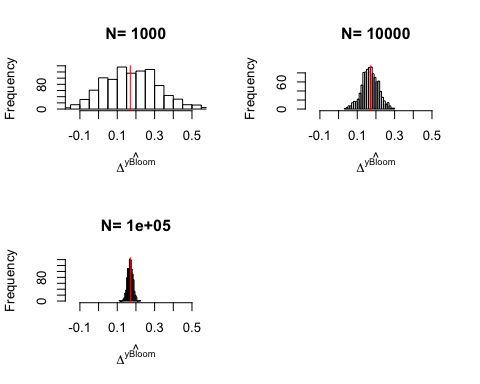
\includegraphics[width=0.5\linewidth]{STCI_files/figure-latex/montecarlohisteligbloom-1} }\subfloat[$Bloom(X)$\label{fig:montecarlohisteligbloom2}]{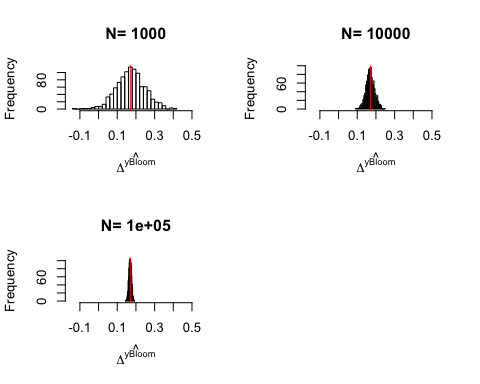
\includegraphics[width=0.5\linewidth]{STCI_files/figure-latex/montecarlohisteligbloom-2} }

}

\caption{Distribution of the $Bloom$ and $Bloom(X)$ estimators with randomization after eligibility over replications of samples of different sizes}\label{fig:montecarlohisteligbloom}
\end{figure}

We can take three things from Figure \ref{fig:montecarlohisteligbloom}:

\begin{enumerate}
\def\labelenumi{\arabic{enumi}.}
\tightlist
\item
  Problems with the IV estimator appear with \(N=100\) (probably because
  there are some samples where no one is treated).
\item
  Sampling noise from randomization after eligibility is indeed larger
  than sampling noise from randomization after self-selection.
\item
  Conditioning on covariates helps.
\end{enumerate}

\subsection{Estimating sampling
noise}\label{estimating-sampling-noise-2}

As always, we can estimate samling noise either using the CLT or
resampling methods. Using the CLT, we can derive the following formula
for the distribution of the Bloom estimator:

\BeginKnitrBlock{theorem}[Asymptotic Distribution of $\hat{\Delta}^Y_{Bloom}$]
\protect\hypertarget{thm:asymBloom}{}{\label{thm:asymBloom}
\iffalse (Asymptotic Distribution of \(\hat{\Delta}^Y_{Bloom}\)) \fi{}
}Under Assumptions \ref{def:indelig}, \ref{def:randeligvalid} and
\ref{def:exclrestric} and assuming that there is at least one individual
with \(R_i=1\) and one individual with \(D_i=1\), we have (keeping the
conditioning on \(E_i=1\) implicit):

\begin{align*}
  \sqrt{N}(\hat{\Delta}^Y_{Bloom}-\Delta^Y_{TT}) &  \stackrel{d}{\rightarrow}
  \mathcal{N}\left(0,\frac{1}{(p^{DR})^2}\left[\left(\frac{p^D}{p^R}\right)^2\frac{\var{Y_i|R_i=0}}{1-p^R}+\left(\frac{1-p^D}{1-p^R}\right)^2\frac{\var{Y_i|R_i=1}}{p^R}\right]\right),
\end{align*}
\EndKnitrBlock{theorem}

with \(p^D=\Pr(D_i=1)\), \(p^R=\Pr(R_i=1)\) and
\((p^{DR}=\Pr(D_i=1|R_i=1)\).

\BeginKnitrBlock{proof}
\iffalse{} {Proof. } \fi{}The proof is immediate using Lemma
\ref{lem:asymWald} in the appendix and setting \(p^{AT}=0\).
\EndKnitrBlock{proof}

\BeginKnitrBlock{remark}
\iffalse{} {Remark. } \fi{}Theorem \ref{thm:asymBloom} shows that there
is a price to pay for not randomizing after self-selection. This price
is a decrease in precision. The variance of the estimator is weighted by
\(\frac{1}{(\Pr(D_i=1|R_i=1))^2}\). This means that the effective sample
size is equal to the number of individuals that take up the treatment
when offered. We generaly call these individuals ``compliers,'' since
they comply with the treatment assignment. Sampling noise is of the same
order of magnitude as the number of compliers You might have very low
precision despite a very large sample size if you have a very small
proportion of compliers.
\EndKnitrBlock{remark}

\BeginKnitrBlock{remark}
\iffalse{} {Remark. } \fi{}In order to compute an estimate of the
sampling noise of hte Bloom estimator, we can either use the plug-in
formula from Theorem \ref{thm:asymBloom} or use the IV standard errors
robust to heteroskedasticity. Here is a simple function in order to
compute the plug-in estimator:
\EndKnitrBlock{remark}

\begin{Shaded}
\begin{Highlighting}[]
\NormalTok{var.RAE.plugin <-}\StringTok{ }\ControlFlowTok{function}\NormalTok{(pDR,pD,pR,V0,V1,N)\{}
  \KeywordTok{return}\NormalTok{(((pD}\OperatorTok{/}\NormalTok{pR)}\OperatorTok{^}\DecValTok{2}\OperatorTok{*}\NormalTok{(V0}\OperatorTok{/}\NormalTok{(}\DecValTok{1}\OperatorTok{-}\NormalTok{pR))}\OperatorTok{+}\NormalTok{((}\DecValTok{1}\OperatorTok{-}\NormalTok{pD)}\OperatorTok{/}\NormalTok{(}\DecValTok{1}\OperatorTok{-}\NormalTok{pR))}\OperatorTok{^}\DecValTok{2}\OperatorTok{*}\NormalTok{(V1}\OperatorTok{/}\NormalTok{pR))}\OperatorTok{/}\NormalTok{(N}\OperatorTok{*}\NormalTok{pDR}\OperatorTok{^}\DecValTok{2}\NormalTok{))}
\NormalTok{\}}
\end{Highlighting}
\end{Shaded}

\BeginKnitrBlock{example}
\protect\hypertarget{exm:unnamed-chunk-104}{}{\label{exm:unnamed-chunk-104}
}Let us derive the CLT-based estimates of sampling noise using both the
plug-in estimator and the IV standard errors without conditioning on
covariates first. For the sake of the example, I'm working with a sample
of size \(N=1000\).
\EndKnitrBlock{example}

\begin{Shaded}
\begin{Highlighting}[]
\NormalTok{sn.RAE.simuls <-}\StringTok{ }\DecValTok{2}\OperatorTok{*}\KeywordTok{quantile}\NormalTok{(}\KeywordTok{abs}\NormalTok{(simuls.elig[[}\StringTok{'1000'}\NormalTok{]][,}\StringTok{'Bloom'}\NormalTok{]}\OperatorTok{-}\NormalTok{delta.y.tt),}\DataTypeTok{probs=}\KeywordTok{c}\NormalTok{(}\FloatTok{0.99}\NormalTok{))}
\NormalTok{sn.RAE.IV.plugin <-}\StringTok{ }\DecValTok{2}\OperatorTok{*}\KeywordTok{qnorm}\NormalTok{((.}\DecValTok{99}\OperatorTok{+}\DecValTok{1}\NormalTok{)}\OperatorTok{/}\DecValTok{2}\NormalTok{)}\OperatorTok{*}\KeywordTok{sqrt}\NormalTok{(}\KeywordTok{var.RAE.plugin}\NormalTok{(}\DataTypeTok{pDR=}\KeywordTok{mean}\NormalTok{(Ds[E}\OperatorTok{==}\DecValTok{1} \OperatorTok{&}\StringTok{ }\NormalTok{R}\OperatorTok{==}\DecValTok{1}\NormalTok{]),}\DataTypeTok{pD=}\KeywordTok{mean}\NormalTok{(Ds[E}\OperatorTok{==}\DecValTok{1}\NormalTok{]),}\DataTypeTok{pR=}\KeywordTok{mean}\NormalTok{(R[E}\OperatorTok{==}\DecValTok{1}\NormalTok{]),}\DataTypeTok{V0=}\KeywordTok{var}\NormalTok{(y[R}\OperatorTok{==}\DecValTok{0} \OperatorTok{&}\StringTok{ }\NormalTok{E}\OperatorTok{==}\DecValTok{1}\NormalTok{]),}\DataTypeTok{V1=}\KeywordTok{var}\NormalTok{(y[R}\OperatorTok{==}\DecValTok{1} \OperatorTok{&}\StringTok{ }\NormalTok{E}\OperatorTok{==}\DecValTok{1}\NormalTok{]),}\DataTypeTok{N=}\KeywordTok{length}\NormalTok{(y[E}\OperatorTok{==}\DecValTok{1}\NormalTok{])))}
\NormalTok{sn.RAE.IV.homo <-}\StringTok{ }\DecValTok{2}\OperatorTok{*}\KeywordTok{qnorm}\NormalTok{((.}\DecValTok{99}\OperatorTok{+}\DecValTok{1}\NormalTok{)}\OperatorTok{/}\DecValTok{2}\NormalTok{)}\OperatorTok{*}\KeywordTok{sqrt}\NormalTok{(}\KeywordTok{vcov}\NormalTok{(reg.y.R.2sls.elig)[}\DecValTok{2}\NormalTok{,}\DecValTok{2}\NormalTok{])}
\NormalTok{sn.RAE.IV.hetero <-}\StringTok{ }\DecValTok{2}\OperatorTok{*}\KeywordTok{qnorm}\NormalTok{((.}\DecValTok{99}\OperatorTok{+}\DecValTok{1}\NormalTok{)}\OperatorTok{/}\DecValTok{2}\NormalTok{)}\OperatorTok{*}\KeywordTok{sqrt}\NormalTok{(}\KeywordTok{vcovHC}\NormalTok{(reg.y.R.2sls.elig,}\DataTypeTok{type=}\StringTok{'HC2'}\NormalTok{)[}\DecValTok{2}\NormalTok{,}\DecValTok{2}\NormalTok{])}
\end{Highlighting}
\end{Shaded}

True 99\% sampling noise (from the simulations) is 0.757. 99\% sampling
noise estimated using the plug-in estimator is 0.921. 99\% sampling
noise estimated using default IV standard errors is 1.069. 99\% sampling
noise estimated using heteroskedasticity robust IV standard errors is
0.92.

Conditioning on covariates:

\begin{Shaded}
\begin{Highlighting}[]
\NormalTok{sn.RAE.simuls.yB <-}\StringTok{ }\DecValTok{2}\OperatorTok{*}\KeywordTok{quantile}\NormalTok{(}\KeywordTok{abs}\NormalTok{(simuls.elig.yB[[}\StringTok{'1000'}\NormalTok{]][,}\StringTok{'Bloom'}\NormalTok{]}\OperatorTok{-}\NormalTok{delta.y.tt),}\DataTypeTok{probs=}\KeywordTok{c}\NormalTok{(}\FloatTok{0.99}\NormalTok{))}
\NormalTok{sn.RAE.IV.homo.yB <-}\StringTok{ }\DecValTok{2}\OperatorTok{*}\KeywordTok{qnorm}\NormalTok{((.}\DecValTok{99}\OperatorTok{+}\DecValTok{1}\NormalTok{)}\OperatorTok{/}\DecValTok{2}\NormalTok{)}\OperatorTok{*}\KeywordTok{sqrt}\NormalTok{(}\KeywordTok{vcov}\NormalTok{(reg.y.R.yB.2sls.elig)[}\DecValTok{2}\NormalTok{,}\DecValTok{2}\NormalTok{])}
\NormalTok{sn.RAE.IV.hetero.yB <-}\StringTok{ }\DecValTok{2}\OperatorTok{*}\KeywordTok{qnorm}\NormalTok{((.}\DecValTok{99}\OperatorTok{+}\DecValTok{1}\NormalTok{)}\OperatorTok{/}\DecValTok{2}\NormalTok{)}\OperatorTok{*}\KeywordTok{sqrt}\NormalTok{(}\KeywordTok{vcovHC}\NormalTok{(reg.y.R.yB.2sls.elig,}\DataTypeTok{type=}\StringTok{'HC2'}\NormalTok{)[}\DecValTok{2}\NormalTok{,}\DecValTok{2}\NormalTok{])}
\end{Highlighting}
\end{Shaded}

True 99\% sampling noise (from the simulations) is 0.393. 99\% sampling
noise estimated using default IV standard errors is 0.457. 99\% sampling
noise estimated using heteroskedasticity robust IV standard errors is
0.454.

\BeginKnitrBlock{remark}
\iffalse{} {Remark. } \fi{}Sampling noise in the Randomization After
Eligibility design seems larger than sampling noise in the Randomization
After Self-Selection design.
\EndKnitrBlock{remark} In the Randomization After Self-Selection design,
sampling noise with \(N=1000\) is equal to 0.55. In the Randomization
After Eligibility design, sampling noise with \(N=1000\) is equal to
0.76. Why such a difference? Both designs have the same effective sample
size.

In the Randomization After Self-Selection design, the effective sample
size \(N^{RASS}_e\) is the number of eligible individuals that apply to
take up the program: \(N^{RASS}_e=N\Pr(D_i=1|E_i=1)\Pr(E_i=1)\). In our
example, \(N^{RASS}_e=1000 *\) 0.459 \(*\) 0.218 \(=\) 100.

In the Randomization After Eligibility design, the sample size on which
the regressions are performed is \(N^{RAE}\), the number of eligible
individuals: \(N^{RAE}=N\Pr(E_i=1)\). In our example, \(N^{RAE}=1000 *\)
0.459 \(=\) 459. But the effective sample size for the Randomization
After Eligibility design is actually equal to the one in the
Randomization After Self-Selection design because only compliers matter
for the precision of the Bloom estimator, as Theorem \ref{thm:asymBloom}
shows. Thus \(N^{RASS}_e=N^{RAE}_e\).

Why then is sampling noise much larger in the Randomization After
Eligibility design? Probably because the Bloom estimator cannot enforce
the fact that the impact of the program on non compliers is zero. It has
to estimate the average outcome of non compliers in both treatment arms
and hope that they cancel. In real samples, they won't, increasing the
size of sampling noise.

\section{Encouragement Design}\label{sec:design4}

In an Encouragement Design, we randomly select two groups among the
eligibles, as in Randomization After Eligibility. Treated individuals
randomly receive an encouragement to participate in the program and
decide whether they want to comply with the encouragement and join the
program. Individuals in the control group do not receive an
encouragement, but they can still decide to self-select in the program.
The Encouragement design differs from the Randomization After
Eligibility design mainly by not barring entry into the programs to
individuals in the control group. If successful, the encouragement
generates a higher level of take up of the program in the treatment
group than in the control group. Examples of encouragements are
additional reminders that the program exists, help in subscribing the
program, financial incentives for subscribing the program, etc.

In an Encouragement Design, we can recover the causal effect of the
treatment not on all the treated but on the treated whose participation
into the program has been triggered by the encouragement. The
individuals reacting to the encouragement by participating in the
program are usually called compliers. The effect of the treatment on the
compliers is called the Local Average Treatment Effect. The main
identification result for Encouragement designs is that a Wald ratio (an
IV estimator) recovers the LATE. It is due to Imbens and Angrist (1994).
A key assumption for this result is exclusion restriction: there has to
be zero impact of the encouragement on the outcome, except through
participation in the treatment. A second key assumption is that no one
individual is driven away from participating in the treatment because of
the encouragement. This assumption is called monotonicity.

Let's detail these assumptions, the identification result and the
estimation strategy.

\subsection{Identification}\label{identification-3}

\subsubsection{Identification of the Local Average Treatment
Effect}\label{identification-of-the-local-average-treatment-effect}

Before stating the identification results, let's go through some
definitions and assumptions. We are going to denote \(R_i=1\) when
individual \(i\) receives the encouragement and \(R_i=0\) when she does
not. As in Section \ref{sec:design3}, we have four potential outcomes
for \(Y_i\): \(Y_i^{d,r}\), \((d,r)\in\left\{0,1\right\}^2\), where
\(d\) denotes receiving the treatment and \(r\) receiving the
encouragement. We also have two potential outcomes for \(D_i\):
\(D_i^{r}\), \(r\in\left\{0,1\right\}\). \(D_i^{1}\) indicates whether
individual \(i\) takes the treatment when receving the encouragement and
\(D_i^{0}\) whether she takes the treatment when not receiving the
encouragement. These potential outcomes define four possible types of
individuals, that I'm going to denote with the random variable \(T_i\):

\begin{itemize}
\tightlist
\item
  \textbf{Always takers}, who take up the program whether they receive
  the encouragement or not. They are such that \(D_i^{1}=D_i^{0}=1\). I
  denote them \(T_i=a\).
\item
  \textbf{Never takers}, who do not take up the program whether they
  receive the encouragement or not. They are such that
  \(D_i^{1}=D_i^{0}=0\). I denote them \(T_i=n\).
\item
  \textbf{Compliers}, who take up the program when they receive the
  encouragement and do not when they do not receive the encouragement.
  They are such that \(D_i^{1}-D_i^{0}=1\). I denote them \(T_i=c\).
\item
  \textbf{Defiers}, who do not take up the program when they receive the
  encouragement and take it up when they do not receive the
  encouragement. They are such that \(D_i^{1}-D_i^{0}=-1\). I denote
  them \(T_i=d\).
\end{itemize}

We are now ready to state the assumptions needed for identification of
the LATE.

\BeginKnitrBlock{definition}[Encouragement Validity]
\protect\hypertarget{def:RandEncouragValid}{}{\label{def:RandEncouragValid}
\iffalse (Encouragement Validity) \fi{} }We assume that the randomized
allocation of the program does not interfere with how potential outcomes
and self-selection are generated:

\begin{align*}
D_i & = D_i^1R_i+(1-R_i)D_i^0 \\
Y_i & = 
  \begin{cases}
    Y_i^{1,1} & \text{ if } (R_i=1 \text{ and } D_i=1)   \\
    Y_i^{0,1} & \text{ if } (R_i=1 \text{ and } D_i=0)    \\
    Y_i^{1,0} & \text{ if } (R_i=0 \text{ and } D_i=1)    \\
    Y_i^{0,0} & \text{ if } (R_i=0 \text{ and } D_i=0)    
  \end{cases}
\end{align*}
\EndKnitrBlock{definition} with \(Y_i^{1,1}\), \(Y_i^{0,1}\),
\(Y_i^{1,0}\), \(Y_i^{0,0}\), \(D_i^1\) and \(D^0_i\) the same potential
outcomes and self-selection decisions as in a routine allocation of the
treatment.

\BeginKnitrBlock{definition}[Independence of Encouragement]
\protect\hypertarget{def:IndepEncourag}{}{\label{def:IndepEncourag}
\iffalse (Independence of Encouragement) \fi{} }We assume that the
randomized allocation of the program is well done:

\begin{align*}
(Y_i^{1,1},Y_i^{0,1},Y_i^{0,0},Y_i^{1,0},D_i^1,D^0_i)\Ind R_i|E_i=1.
\end{align*}
\EndKnitrBlock{definition}

\BeginKnitrBlock{definition}[Exclusion Restriction]
\protect\hypertarget{def:ExclRestr}{}{\label{def:ExclRestr}
\iffalse (Exclusion Restriction) \fi{} }We assume that the randomized
allocation of the program does not alter potential outcomes:

\begin{align*}
Y_i^{d,r} & = Y_i^d \text{, }\forall (r,d)\in\left\{0,1\right\}^2.
\end{align*}
\EndKnitrBlock{definition}

\BeginKnitrBlock{definition}[First Stage]
\protect\hypertarget{def:Fstage}{}{\label{def:Fstage} \iffalse (First Stage)
\fi{} }We assume that the encouragement does manage to increase
participation:

\begin{align*}
  \Pr(D_i=1|R_i=1,E_i=1) > \Pr(D_i=1|R_i=0,E_i=1).
\end{align*}
\EndKnitrBlock{definition}

\BeginKnitrBlock{definition}[Monotonicity]
\protect\hypertarget{def:Mono}{}{\label{def:Mono} \iffalse (Monotonicity)
\fi{} }We assume that the encouragement either increases participation
for everyone or decreases participation for everyone:

\begin{align*}
  \text{ either } \forall i\text{, }D_i^1\geq D_i^0 \text{ or } \forall i\text{, }D_i^1\leq D_i^0 .
\end{align*}
\EndKnitrBlock{definition}

Assumption \ref{def:Mono} means that we cannot have simultaneously
individuals that are pushed by the encouragement into the treatment and
individuals that are pushed out of the treatment. As a consequence,
there cannot be compliers and defiers at the same time. There can only
be compliers or defiers. For simplicity, in what follows, I assume that
there are no defiers. This is without loss of generality, since, under
Assumption \ref{def:Mono}, a redefinition of the treatment
(\(\tilde{D}_i=-D_i\)) moves the model in this section from one with
only defiers to one with only compliers.

\BeginKnitrBlock{theorem}[Identification in an Encouragement Design]
\protect\hypertarget{thm:IdentLATE}{}{\label{thm:IdentLATE}
\iffalse (Identification in an Encouragement Design) \fi{} }Under
Assumptions \ref{def:RandEncouragValid}, \ref{def:IndepEncourag},
\ref{def:ExclRestr}, \ref{def:Fstage} and \ref{def:Mono}, the Wald
estimator identifies the LATE:

\begin{align*}
  \Delta^Y_{Wald} & = \Delta^Y_{LATE},
\end{align*}
\EndKnitrBlock{theorem}

with:

\begin{align*}
  \Delta^Y_{Wald} & = \frac{\esp{Y_i|R_i=1,E_i=1} - \esp{Y_i|R_i=0,E_i=1}}{\Pr(D_i=1|R_i=1,E_i=1)-\Pr(D_i=1|R_i=0,E_i=1)}\\
  \Delta^Y_{LATE} & = \esp{Y^1_i-Y^0_i|T_i=c,E_i=1}.
\end{align*}

\BeginKnitrBlock{proof}
\iffalse{} {Proof. } \fi{}See Section \ref{proofIdentLATE}.
\EndKnitrBlock{proof}

\BeginKnitrBlock{remark}
\iffalse{} {Remark. } \fi{}Theorem \ref{thm:IdentLATE} is pretty
amazing. It shows that there exists a set of assumptions under which we
can use an encouragement design to recover the effect of the treatment
(\(D_i\)) on outcomes, despite the fact that we have NOT randomized
\(D_i\). The assumptions needed for that to happen are intuitive:
\EndKnitrBlock{remark}

\begin{enumerate}
\def\labelenumi{\arabic{enumi}.}
\tightlist
\item
  The encouragement has to have no direct effect on the outcomes
  (Assumption \ref{def:ExclRestr})
\item
  The encouragement has to have an effect on treatment uptake
  (Assumption \ref{def:Fstage})
\item
  The encouragement does not generate two-way flows in and out of the
  treatment, but only a one-way flow (Assumption \ref{def:Mono})
\end{enumerate}

Under these assumptions, the only way that we can see a difference in
outcomes between those that receive the encouragement and those that do
not is that the treatment has had an effect on those that have taken it
because of the encouragement. It cannot be because of the encouragement
itself, because of Assumption \ref{def:ExclRestr}. It cannot be because
some people with particularly low outcomes have exited the program
because of the encouragement, Assumption \ref{def:Mono} forbids it. And
if we see no effect of the encouragement, it has to be that the
treatment has no effect on the compliers as well, because Assumption
\ref{def:Fstage} implies that they have received the treatment in the
encouragement group and that they have not in the group without
encouragement.

\BeginKnitrBlock{remark}
\iffalse{} {Remark. } \fi{}Less nice with Theorem \ref{thm:IdentLATE} is
that we recover the effect only for a subgroup of individuals, the
compliers. This raises two issues:
\EndKnitrBlock{remark}

\begin{enumerate}
\def\labelenumi{\arabic{enumi}.}
\tightlist
\item
  The effect on the compliers (or LATE) is not the effect on the treated
  (TT). When the treatment is given in routine mode, without the
  encouragement, TT is actually equal to the effect on the always
  takers. There is nothing that tells us that the always takers react in
  the same way to the treatment as the compliers. As soon as the
  expected benefits of the treatment enter the decision of taking it up,
  always takers have larger treatment effects than compliers.
\item
  The identity of the compliers is unobserved. We cannot decide to
  allocate the treatment only to the compliers because they are defined
  by their counterfactual response to the encouragement. In both
  treatment arms, we do not know who the compliers are. We know they are
  among those who take up the program in the group receiving the
  encouragement. But there are also always takers that take up the
  program in this group. We know that they are among those that do not
  take up the program in the group that does not receive the
  encouragement. But never takers behave in the same way in that group.
\end{enumerate}

The only way to direct the treatment at the compliers is to use the
encouragement. So, we end up evaluating the effect of the encouragement
itself and not of the program. In that case, we do not need Assumptions
\ref{def:ExclRestr}, \ref{def:Fstage} and \ref{def:Mono}, because they
are not needed to identify the effect of the encouragement (see Section
\ref{ITEEncourag} below).

In general, researchers believe that LATE tells them something about the
magnitude of the effect beyond compliers. This is not warranted by the
maths, but one can understand how a bayesian decision-maker may use the
information from some subpopulation to infer what would happen to
another. Comparing LATEs and TTs for similar treatments is an active
area for reasearch. I know of no paper doing that extensively and
nicely.

To generalize from the LATE to the TT, we can make the assumption that
the impact on always takers is equal to the impact on compliers, but
that seems a little far-fetched.
\href{https://www.nber.org/papers/w16566}{Angrist and Fernandez-Val}
propose to assume that the effect on compliers is equal to the effect on
always takers conditional on some observed covariates. When outcomes are
bounded (for example because they are between zero and one), we can try
to bound the \(TT\) using the \(LATE\) (see
\href{https://onlinelibrary.wiley.com/doi/abs/10.1002/jae.2473}{Huber,
Laffers and Mellace (2017)}).

\BeginKnitrBlock{remark}
\iffalse{} {Remark. } \fi{}If you see a connexion between the conditions
for the Wald estimator to identify LATE and the assumptions behind an IV
estimator, you're correct. The Wald estimator is actually an IV
estimator (see Lemma \ref{lem:WaldIV} below).
\EndKnitrBlock{remark}

\subsubsection{Identification of the Intention to Treat
Effect}\label{ITEEncourag}

In this section, we are going to delineate how to identify the Intention
to Treat Effect (ITE) in an Encouragement design. In an Encouragement
design, ITE is the effect of receiving the encouragement. It is defined
in a similar manner as in a Randomization After Eligibility design (see
Definition \ref{def:ITE}):
\(\Delta^Y_{ITE} = \esp{Y_i^{D_i^1,1}-Y_i^{D_i^0,0}|E_i=1}\).

Under Assumption \ref{def:RandEncouragValid}, receiving the
encouragement has several impacts:

\begin{enumerate}
\def\labelenumi{\arabic{enumi}.}
\tightlist
\item
  Some individuals (the compliers) decide to enter the program,
\item
  Some individuals (the defiers) decide to exit the program,
\item
  The encouragement might have a direct effect on outcomes
  (\(Y_i^{d,1}\neq Y_i^{d,0}\)).
\end{enumerate}

This last effect is the effect of receiving the encouragement that does
not goes through participation into the program. For example, it is
possible that sending an encouragement to take up a retirement program
makes me save more for retirement, even if I end up not taking up the
proposed program.

The two causal channels that are at work within the ITE can be seen more
clearly when decomposing the ITE to make each type appear. We can do
that because the four types define a partition of the sample space, that
is a collection of mutually exclusive events whose union spans the whole
space. As a consequence of that, conditioning on the union of the four
types is the same thing as not conditioning on anything. Using this
trick, we have:

\begin{align}
  \Delta^Y_{ITE} & = \esp{Y_i^{D_i^1,1}-Y_i^{D_i^0,0}|(T_i=a\cup T_i=c\cup T_i=d\cup T_i=n)\cap E_i=1}\nonumber\\
                & = \esp{Y_i^{D_i^1,1}-Y_i^{D_i^0,0}|T_i=a,E_i=1}\Pr(T_i=a|E_i=1)\nonumber\\
                & \phantom{=}+ \esp{Y_i^{D_i^1,1}-Y_i^{D_i^0,0}|T_i=c,E_i=1}\Pr(T_i=c|E_i=1)\nonumber\\
                & \phantom{=}+ \esp{Y_i^{D_i^1,1}-Y_i^{D_i^0,0}|T_i=d,E_i=1}\Pr(T_i=d|E_i=1)\nonumber\\
                & \phantom{=}+ \esp{Y_i^{D_i^1,1}-Y_i^{D_i^0,0}|T_i=n,E_i=1}\Pr(T_i=n|E_i=1)\nonumber\\
                & = \esp{Y_i^{1,1}-Y_i^{1,0}|T_i=a,E_i=1}\Pr(T_i=a|E_i=1)\nonumber\\
                & \phantom{=}+ \esp{Y_i^{1,1}-Y_i^{0,0}|T_i=c,E_i=1}\Pr(T_i=c|E_i=1)\nonumber\\
                & \phantom{=}+ \esp{Y_i^{0,1}-Y_i^{1,0}|T_i=d,E_i=1}\Pr(T_i=d|E_i=1)\nonumber\\
                & \phantom{=}+ \esp{Y_i^{0,1}-Y_i^{0,0}|T_i=n,E_i=1}\Pr(T_i=n|E_i=1),\label{eq:ITE3}
\end{align}

where the first equality follows from the four types defining a
partition of the sample space, the second equality from the usual rule
of conditional expectations and the fact that types are disjoint events,
and the third equality from Assumption \ref{def:randeligvalid}.

We can now see that ITE is composed of four terms:

\begin{enumerate}
\def\labelenumi{\arabic{enumi}.}
\tightlist
\item
  The effect of receiving the encouragment on the always takers. This
  effect is only the direct effect of the encouragement, and not the
  effect of the program since the always takers always take the program.
  This term cancels under Assumption \ref{def:ExclRestr}, when there is
  no direct effect of the encouragement on outcomes.
\item
  The effect of receiving the encouragement on compliers. This is both
  the effect of the encouragement and of the program. This is equal to
  the LATE under Assumption \ref{def:ExclRestr}.
\item
  The effect of receiving the encouragement on defiers. This is the
  difference between the direct effect of the encouragement and the
  effect of the program. This is equal to the opposite of the effect of
  the treatment on the defiers under Assumption \ref{def:ExclRestr}.
\item
  The effect of receiving the encouragement on never takers. This effect
  is only the direct effect of the encouragement, and not the effect of
  the program since the never takers never take the program. This term
  cancels under Assumption \ref{def:ExclRestr}.
\end{enumerate}

All these effects are weighted by the respective proportions of the
types in the population. ITE is linked to LATE. This link can be made
clearer:

\BeginKnitrBlock{theorem}[From ITE to Compliers and Defiers]
\protect\hypertarget{thm:ITELATE}{}{\label{thm:ITELATE} \iffalse (From ITE
to Compliers and Defiers) \fi{} }Under Assumptions
\ref{def:RandEncouragValid} and \ref{def:ExclRestr}, ITE is equal to the
effect on compliers minus the effect on defiers weighted by their
respective proportions in the population:

\begin{align*}
  \Delta^Y_{ITE} & = \esp{Y_i^{1}-Y_i^{0}|T_i=c,E_i=1}\Pr(T_i=c|E_i=1)\\
                  & \phantom{=}-\esp{Y_i^{1}-Y_i^{0}|T_i=d,E_i=1}\Pr(T_i=d|E_i=1).
\end{align*}
\EndKnitrBlock{theorem}

\BeginKnitrBlock{proof}
\iffalse{} {Proof. } \fi{}Under Assumption \ref{def:ExclRestr}, Equation
\eqref{eq:ITE3} becomes:

\begin{align*}
  \Delta^Y_{ITE} & = \esp{Y_i^{1}-Y_i^{1}|T_i=a,E_i=1}\Pr(T_i=a|E_i=1)\\
                & \phantom{=}+ \esp{Y_i^{1}-Y_i^{0}|T_i=c,E_i=1}\Pr(T_i=c|E_i=1)\\
                & \phantom{=}+ \esp{Y_i^{0}-Y_i^{1}|T_i=d,E_i=1}\Pr(T_i=d|E_i=1)\\
                & \phantom{=}+ \esp{Y_i^{0}-Y_i^{0}|T_i=n,E_i=1}\Pr(T_i=n|E_i=1)
\end{align*}

which proves the result.
\EndKnitrBlock{proof}

The previous theorem shows that Assumption \ref{def:ExclRestr} shuts
down any direct effect of receiving the encouragement on outcomes. As a
consequence of this assumption, the only impact that receiving the
encouragement has on outcomes is through participation into the program.
Hence, ITE is equal to the impact of the program on those who react to
the encouragement: the compliers and the defiers, weighted by their
respective proportions.

The problem with the result of Theorem \ref{thm:ITELATE} is that ITE
contains two-way flows in and out of the program. If we want to know
something about the effect of the program, and not only about the effect
of the encouragement, we need to assume that defiers do not exist.
That's what Assumption \ref{def:Mono} does, as the following theorem
shows:

\BeginKnitrBlock{theorem}[From ITE to LATE]
\protect\hypertarget{thm:ITELATEMono}{}{\label{thm:ITELATEMono}
\iffalse (From ITE to LATE) \fi{} }Under Assumptions
\ref{def:RandEncouragValid}, \ref{def:ExclRestr} and \ref{def:Mono}, ITE
is equal to the LATE multiplied by the proportion of compliers in the
population:

\begin{align*}
  \Delta^Y_{ITE} & = \Delta^Y_{LATE}\Pr(T_i=c|E_i=1).
\end{align*}
\EndKnitrBlock{theorem}

\BeginKnitrBlock{proof}
\iffalse{} {Proof. } \fi{}The result is straighforward using Assumption
\ref{def:Mono} and Theorem \ref{thm:ITELATE}. Indeed, Assumption
\ref{def:Mono} implies that \(\forall i\), \(D_i^1-D_i^0\geq 0\)
(choosing only the first ``either'' statement, without loss of
generality). As a consequence,
\(\Pr(T_i=d|E_i=1)=\Pr(D_i^1-D_i^0=-1|E_i=1)=0\).
\EndKnitrBlock{proof}

In order to move from the link between LATE and ITE to the mechanics of
the Wald estimator, we need two additional identification results. The
first result shows that ITE can be identified under fairly light
conditions by a WW estimator. The second result shows that the
proportion of people taking up the treatment when eligiblity is
announced is also easily estimated from the data.

\BeginKnitrBlock{theorem}[Identification of ITE in an Encouragement Design]
\protect\hypertarget{thm:ITEEncourag}{}{\label{thm:ITEEncourag}
\iffalse (Identification of ITE in an Encouragement Design) \fi{} }Under
Assumptions \ref{def:RandEncouragValid} and \ref{def:IndepEncourag}, ITE
is identified by the With/Without comparison among eligibles:

\begin{align*}
  \Delta^Y_{ITE} & = \Delta^Y_{WW|E_i=1}.
\end{align*}
\EndKnitrBlock{theorem}

\BeginKnitrBlock{proof}
\iffalse{} {Proof. } \fi{}

\begin{align*}
 \Delta^Y_{WW|E=1} & =\esp{Y_i|R_i=1,E_i=1}-\esp{Y_i|R_i=0,E_i=1} \\
                   & = \esp{Y_i^{D_i^1,1}|R_i=1,E_i=1}-\esp{Y_i^{D_i^0,0}|R_i=0,E_i=1} \\
                    & = \esp{Y_i^{D_i^1,1}|E_i=1}-\esp{Y_i^{D_i^0,0}|E_i=1},
\end{align*}

where the second equality follows from Assumption
\ref{def:RandEncouragValid} and the third from Assumption
\ref{def:IndepEncourag}.
\EndKnitrBlock{proof}

\BeginKnitrBlock{theorem}[Identification of the Proportion of Compliers]
\protect\hypertarget{thm:prEncourag}{}{\label{thm:prEncourag}
\iffalse (Identification of the Proportion of Compliers) \fi{} }Under
Assumptions \ref{def:RandEncouragValid}, \ref{def:IndepEncourag} and
\ref{def:Mono}, the proportion of compliers is identified by the
difference between the proportion of people taking up the program among
those receiving the encouragement and the proportion of individuals
taking up the program among those not receiving the encouragement:

\begin{align*}
  \Pr(T_i=c|E_i=1) & = \Pr(D_i=1|R_i=1,E_i=1)-\Pr(D_i=1|R_i=0,E_i=1).
\end{align*}
\EndKnitrBlock{theorem}

\BeginKnitrBlock{proof}
\iffalse{} {Proof. } \fi{}

\begin{align*}
 \Pr(D_i=1|R_i=1,E_i=1) & =\Pr(D_i=1\cap (T_i=a\cup T_i=c\cup T_i=d\cup T_i=n)|R_i=1,E_i=1) \\
                        & = \Pr(D_i=1\cap T_i=a|R_i=1,E_i=1)\\
                        & \phantom{=}+ \Pr(D_i=1\cap T_i=c|R_i=1,E_i=1)\\
                        & \phantom{=} +\Pr(D_i=1\cap T_i=d|R_i=1,E_i=1)\\
                        & \phantom{=} +\Pr(D_i=1\cap T_i=n|R_i=1,E_i=1)\\
                        & = \Pr(T_i=a|R_i=1,E_i=1)\\
                        & \phantom{=} +\Pr(T_i=c|R_i=1,E_i=1)\\
                        & = \Pr(T_i=a|E_i=1)\\
                        & \phantom{=} +\Pr(T_i=c|E_i=1),
\end{align*}

where the first equality follows the types being a partition of the
sample space; the second equality from the fact that the types are
disjoint sets; the third equality from the fact that
\(T_i=a|R_i=1 \Rightarrow D_i=1\) (so that
\(\Pr(D_i=1\cap T_i=a|R_i=1,E_i=1)=\Pr(T_i=a|R_i=1,E_i=1)\)),
\(T_i=c|R_i=1 \Rightarrow D_i=1\) (so that
\(\Pr(D_i=1\cap T_i=c|R_i=1,E_i=1)=\Pr(T_i=c|R_i=1,E_i=1)\)),
\(T_i=d|R_i=1 \Rightarrow D_i=0\) (so that
\(\Pr(D_i=1\cap T_i=d|R_i=1,E_i=1)=0\)) and
\(T_i=n|R_i=1 \Rightarrow D_i=0\) (so that
\(\Pr(D_i=1\cap T_i=n|R_i=1,E_i=1)=0\)); and the fourth equality from
Assumption \ref{def:IndepEncourag} and Lemma \ref{lem:UnconfTypes}.
\EndKnitrBlock{proof}

\BeginKnitrBlock{corollary}[Wald estimator and ITE]
\protect\hypertarget{cor:EncouragWald}{}{\label{cor:EncouragWald}
\iffalse (Wald estimator and ITE) \fi{} }It follows from Theorems
\ref{thm:ITEEncourag} and \ref{thm:prEncourag} that, under Assumptions
\ref{def:RandEncouragValid}, \ref{def:IndepEncourag} and \ref{def:Mono},
the Wald estimator is equal to the ITE divided by the propotion of
compliers:

\begin{align*}
  \Delta^Y_{Wald|E=1} & = \frac{\Delta^Y_{ITE}}{\Pr(T_i=c|E_i=1)}.
\end{align*}
\EndKnitrBlock{corollary}

As a consequence of Corollary \ref{cor:EncouragWald}, we see that the
Wald estimator reweights the ITE, the effect of receiving an
encouragement, by the proportion of people reacting to the encouragement
by participating in the program, the compliers. From Theorem
\ref{thm:ITELATE}, we know that this ratio will be equal to LATE if the
Assumption \ref{def:ExclRestr} also holds, so that all the impact of the
encouragement stems from entering the program. The encouragement serves
as an instrument for program participation.

\BeginKnitrBlock{remark}
\iffalse{} {Remark. } \fi{}The Encouragement design seems like magic.
You do not assign randomly the program, but only an encouragement to
take it, and you can recover the effect of the program anyway. The
Encouragement design is less intrusive than Randomization After
Self-Selection and Randomization of Eligibility. In an Encouragement
design, you do not have to refuse the program to agents in the control
group. You pay two types of prices for that:
\EndKnitrBlock{remark}

\begin{enumerate}
\def\labelenumi{\arabic{enumi}.}
\tightlist
\item
  You only recover LATE, not TT
\item
  You have larger sampling noise.
\end{enumerate}

The intuition for this second point can be delineated using the very
same apparatus that we have developed so far. So here goes. Under the
assumptions made so far, it is easy to show that (omitting the
conditioning on \(E_i=1\) for simplicity):

\begin{align*}
  \Delta^Y_{WW|E=1} & = \esp{Y_i^{1,1}|T_i=a,R_i=1}\Pr(T_i=a,|R_i=1)\\
                    & \phantom{=}-\esp{Y_i^{1,0}|T_i=a,R_i=0}\Pr(T_i=a,|R_i=0)\\
                    & \phantom{=}+ \esp{Y_i^{1,1}|T_i=c,R_i=1}\Pr(T_i=c|R_i=1)\\
                    & \phantom{=}-\esp{Y_i^{0,0}|T_i=c,R_i=0}\Pr(T_i=c|R_i=0)\\
                    & \phantom{=}+ \esp{Y_i^{0,1}|T_i=d,R_i=1}\Pr(T_i=d|R_i=1)\\
                    & \phantom{=}-\esp{Y_i^{1,0}|T_i=d,R_i=0}\Pr(T_i=d|R_i=0)\\
                    & \phantom{=}+ \esp{Y_i^{0,1}|T_i=n,R_i=1}\Pr(T_i=n|R_i=1)\\
                    & \phantom{=}-\esp{Y_i^{0,0}|T_i=n,R_i=0}\Pr(T_i=n|R_i=0).
\end{align*}

The four parts of the equation account for comparisons among each type
between the two treatment arms. The parts due to always takers and never
takers cancel out under Assumptions \ref{def:IndepEncourag} and
\ref{def:ExclRestr}. But this cancelling out only happens in the
population. In a given sample, the sample equivalents of the two members
of each difference do not have to be equal, and thus they do not cancel
out, generating sampling noise. Ideally, we would like to enforce that
the effect of the encouragement on always takers and never takers is
null, as Assumption \ref{def:ExclRestr} imposes, but that would require
observing the type variable \(T_i\). Unfortunately, we cannot now the
type of each individual in the sample, since it is defined
counterfactually. Maybe someday we'll be able to use prior responses to
the encouragement to identify the type of each individual and thus
improve the precision of the Wald estimator.

\textbf{\textsc{Explain de Chaisemartin.}}

\BeginKnitrBlock{remark}
\iffalse{} {Remark. } \fi{}what if we fear there are defiers. de
Chaisemartin
\EndKnitrBlock{remark}

\BeginKnitrBlock{remark}
\iffalse{} {Remark. } \fi{}In practice, we use a pseudo-RNG to allocate
the randomized annoucement of the encouragement:
\EndKnitrBlock{remark}

\begin{align*}
  R_i^* & \sim \mathcal{U}[0,1]\\
  R_i & = 
  \begin{cases}
    1 & \text{ if } R_i^*\leq .5 \land E_i=1\\
    0 & \text{ if } R_i^*> .5 \land E_i=1
  \end{cases} \\
  D_i & = \uns{\bar{\alpha}+\theta\bar{\mu}+\psi R_i-C_i\geq0 \land E_i=1}
\end{align*}

\(\psi\) denotes the increase in agents' valuation of the program after
receiving the encouragement.

\BeginKnitrBlock{example}
\protect\hypertarget{exm:unnamed-chunk-117}{}{\label{exm:unnamed-chunk-117}
}Let's see how the encouragement design works in our numerical example.
Let's choose a value for \(\psi\) and add it to the vector of
parameters.
\EndKnitrBlock{example}

\begin{Shaded}
\begin{Highlighting}[]
\NormalTok{param <-}\StringTok{ }\KeywordTok{c}\NormalTok{(param,}\FloatTok{0.6}\NormalTok{)}
\KeywordTok{names}\NormalTok{(param) <-}\StringTok{ }\KeywordTok{c}\NormalTok{(}\StringTok{"barmu"}\NormalTok{,}\StringTok{"sigma2mu"}\NormalTok{,}\StringTok{"sigma2U"}\NormalTok{,}\StringTok{"barY"}\NormalTok{,}\StringTok{"rho"}\NormalTok{,}\StringTok{"theta"}\NormalTok{,}\StringTok{"sigma2epsilon"}\NormalTok{,}\StringTok{"sigma2eta"}\NormalTok{,}\StringTok{"delta"}\NormalTok{,}\StringTok{"baralpha"}\NormalTok{,}\StringTok{"barc"}\NormalTok{,}\StringTok{"gamma"}\NormalTok{,}\StringTok{"sigma2V"}\NormalTok{,}\StringTok{"psi"}\NormalTok{)}
\end{Highlighting}
\end{Shaded}

Let's first compute the value of LATE in this new model. Let's denote
\(D_i^{*0}=\bar{\alpha}+\theta\bar{\mu}-C_i\) the utility of agent \(i\)
absent the encouragement, with \(C_i=\bar{c} + \gamma \mu_i + V_i\). In
order to be a complier, you have to have a utility of the program that
is insufficient to make you apply for the program when you receive no
encouragement (\(D_i^{*0}<0\)) and a positive utility of applying to the
treatment after receiving the encouragement (\(D_i^{*0}+\psi\geq 0\)).
Compliers are thus such that \(-\psi\leq D_i^{*0}<0\). LATE can thus be
written as follows in our model:

\begin{align*}
  \Delta^y_{LATE} & = \bar{\alpha}+ \theta\esp{\mu_i|\mu_i+U_i^B\leq\bar{y} \land -\psi\leq D_i^{*0}<0},
\end{align*}

Using the same approach, we can also compute the proportion of compliers
among eligibles. In our model, we indeed have:

\begin{align*}
  \Pr(T_i=c|E_i=1) & = \Pr(-\psi\leq D_i^{*0}<0|\mu_i+U_i^B\leq\bar{y}).
\end{align*}

Since all errors terms are normally distributed in our model, we can
compute the package \texttt{tmvtnorm} to compute both LATE and the
proportion of compliers among eligibles.

\begin{align*}
  (\mu_i,y_i^B,D_i^{*0}) & = \mathcal{N}\left(\bar{\mu},\bar{\mu},\bar{\alpha}+(\theta-\gamma)\bar{\mu}-\bar{c},
                                        \left(\begin{array}{ccc}
                                              \sigma^2_{\mu} & \sigma^2_{\mu} & -\gamma\sigma^2_{\mu} \\
                                              \sigma^2_{\mu} & \sigma^2_{\mu} + \sigma^2_{U} & -\gamma\sigma^2_{\mu} \\
                                              -\gamma\sigma^2_{\mu} & -\gamma\sigma^2_{\mu} & \gamma^2\sigma^2_{\mu}+\sigma^2_{V}
                                              \end{array}
                                        \right)
                                      \right)
\end{align*}

\begin{Shaded}
\begin{Highlighting}[]
\NormalTok{mean.mu.yB.Dstar <-}\StringTok{ }\KeywordTok{c}\NormalTok{(param[}\StringTok{'barmu'}\NormalTok{],param[}\StringTok{'barmu'}\NormalTok{],param[}\StringTok{'baralpha'}\NormalTok{]}\OperatorTok{-}\StringTok{ }\NormalTok{param[}\StringTok{'barc'}\NormalTok{]}\OperatorTok{+}\NormalTok{(param[}\StringTok{'theta'}\NormalTok{]}\OperatorTok{-}\NormalTok{param[}\StringTok{'gamma'}\NormalTok{])}\OperatorTok{*}\NormalTok{param[}\StringTok{'barmu'}\NormalTok{])}
\NormalTok{cov.mu.yB.Dstar <-}\StringTok{ }\KeywordTok{matrix}\NormalTok{(}\KeywordTok{c}\NormalTok{(param[}\StringTok{'sigma2mu'}\NormalTok{],param[}\StringTok{"sigma2mu"}\NormalTok{],}\OperatorTok{-}\NormalTok{param[}\StringTok{'gamma'}\NormalTok{]}\OperatorTok{*}\NormalTok{param[}\StringTok{"sigma2mu"}\NormalTok{],}
\NormalTok{                            param[}\StringTok{"sigma2mu"}\NormalTok{],param[}\StringTok{'sigma2mu'}\NormalTok{]}\OperatorTok{+}\NormalTok{param[}\StringTok{'sigma2U'}\NormalTok{],}\OperatorTok{-}\NormalTok{param[}\StringTok{'gamma'}\NormalTok{]}\OperatorTok{*}\NormalTok{param[}\StringTok{"sigma2mu"}\NormalTok{],}
                            \OperatorTok{-}\NormalTok{param[}\StringTok{'gamma'}\NormalTok{]}\OperatorTok{*}\NormalTok{param[}\StringTok{"sigma2mu"}\NormalTok{],}\OperatorTok{-}\NormalTok{param[}\StringTok{'gamma'}\NormalTok{]}\OperatorTok{*}\NormalTok{param[}\StringTok{"sigma2mu"}\NormalTok{],param[}\StringTok{"sigma2mu"}\NormalTok{]}\OperatorTok{*}\NormalTok{(param[}\StringTok{'gamma'}\NormalTok{])}\OperatorTok{^}\DecValTok{2}\OperatorTok{+}\NormalTok{param[}\StringTok{'sigma2V'}\NormalTok{]),}\DecValTok{3}\NormalTok{,}\DecValTok{3}\NormalTok{,}\DataTypeTok{byrow=}\OtherTok{TRUE}\NormalTok{)}
\CommentTok{# late}
\NormalTok{lower.cut <-}\StringTok{ }\KeywordTok{c}\NormalTok{(}\OperatorTok{-}\OtherTok{Inf}\NormalTok{,}\OperatorTok{-}\OtherTok{Inf}\NormalTok{,}\OperatorTok{-}\NormalTok{param[}\StringTok{'psi'}\NormalTok{])}
\NormalTok{upper.cut <-}\StringTok{ }\KeywordTok{c}\NormalTok{(}\OtherTok{Inf}\NormalTok{,}\KeywordTok{log}\NormalTok{(param[}\StringTok{'barY'}\NormalTok{]),}\DecValTok{0}\NormalTok{)}
\NormalTok{moments.cut <-}\StringTok{ }\KeywordTok{mtmvnorm}\NormalTok{(}\DataTypeTok{mean=}\NormalTok{mean.mu.yB.Dstar,}\DataTypeTok{sigma=}\NormalTok{cov.mu.yB.Dstar,}\DataTypeTok{lower=}\NormalTok{lower.cut,}\DataTypeTok{upper=}\NormalTok{upper.cut)}
\NormalTok{delta.y.late <-}\StringTok{ }\NormalTok{param[}\StringTok{'baralpha'}\NormalTok{]}\OperatorTok{+}\StringTok{ }\NormalTok{param[}\StringTok{'theta'}\NormalTok{]}\OperatorTok{*}\NormalTok{moments.cut}\OperatorTok{$}\NormalTok{tmean[}\DecValTok{1}\NormalTok{]}
\CommentTok{# proportion of compliers}
\NormalTok{lower.cut <-}\StringTok{ }\KeywordTok{c}\NormalTok{(}\OperatorTok{-}\OtherTok{Inf}\NormalTok{,}\OperatorTok{-}\OtherTok{Inf}\NormalTok{,}\OperatorTok{-}\OtherTok{Inf}\NormalTok{)}
\NormalTok{upper.cut <-}\StringTok{ }\KeywordTok{c}\NormalTok{(}\OtherTok{Inf}\NormalTok{,}\KeywordTok{log}\NormalTok{(param[}\StringTok{'barY'}\NormalTok{]),}\OtherTok{Inf}\NormalTok{)}
\NormalTok{pr.compliers <-}\StringTok{ }\KeywordTok{ptmvnorm.marginal}\NormalTok{(}\DataTypeTok{xn=}\DecValTok{0}\NormalTok{,}\DataTypeTok{n=}\DecValTok{3}\NormalTok{,}\DataTypeTok{mean=}\NormalTok{mean.mu.yB.Dstar,}\DataTypeTok{sigma=}\NormalTok{cov.mu.yB.Dstar,}\DataTypeTok{lower=}\NormalTok{lower.cut,}\DataTypeTok{upper=}\NormalTok{upper.cut)}\OperatorTok{-}\KeywordTok{ptmvnorm.marginal}\NormalTok{(}\DataTypeTok{xn=}\OperatorTok{-}\NormalTok{param[}\StringTok{'psi'}\NormalTok{],}\DataTypeTok{n=}\DecValTok{3}\NormalTok{,}\DataTypeTok{mean=}\NormalTok{mean.mu.yB.Dstar,}\DataTypeTok{sigma=}\NormalTok{cov.mu.yB.Dstar,}\DataTypeTok{lower=}\NormalTok{lower.cut,}\DataTypeTok{upper=}\NormalTok{upper.cut)}
\NormalTok{delta.y.ite <-}\StringTok{ }\NormalTok{delta.y.late}\OperatorTok{*}\NormalTok{pr.compliers}
\end{Highlighting}
\end{Shaded}

The value of \(\Delta^y_{LATE}\) in the population is thus 0.173. The
proportion of compliers among eligibles in the population is 0.272. As a
consequence of Corollary \ref{cor:EncouragWald}, we can compute ITE as
the product of LATE and the proportion of compliers. In our example, ITE
is thus equal to 0.047 in the population.

Now let's simulate a new sample with the encouragement delivered
randomly among eligibles. I'm also defining the potential outcomes
\(D^1_i\) and \(D^0_i\) and the types \(T_i\) for later use.

\begin{Shaded}
\begin{Highlighting}[]
\CommentTok{# I'm changing the seed because with the usual one, I get a negative estimate of the treatment effect: lots of sampling noise!}
\KeywordTok{set.seed}\NormalTok{(}\DecValTok{12345}\NormalTok{)}
\NormalTok{N <-}\DecValTok{1000}
\NormalTok{mu <-}\StringTok{ }\KeywordTok{rnorm}\NormalTok{(N,param[}\StringTok{"barmu"}\NormalTok{],}\KeywordTok{sqrt}\NormalTok{(param[}\StringTok{"sigma2mu"}\NormalTok{]))}
\NormalTok{UB <-}\StringTok{ }\KeywordTok{rnorm}\NormalTok{(N,}\DecValTok{0}\NormalTok{,}\KeywordTok{sqrt}\NormalTok{(param[}\StringTok{"sigma2U"}\NormalTok{]))}
\NormalTok{yB <-}\StringTok{ }\NormalTok{mu }\OperatorTok{+}\StringTok{ }\NormalTok{UB }
\NormalTok{YB <-}\StringTok{ }\KeywordTok{exp}\NormalTok{(yB)}
\NormalTok{epsilon <-}\StringTok{ }\KeywordTok{rnorm}\NormalTok{(N,}\DecValTok{0}\NormalTok{,}\KeywordTok{sqrt}\NormalTok{(param[}\StringTok{"sigma2epsilon"}\NormalTok{]))}
\NormalTok{eta<-}\StringTok{ }\KeywordTok{rnorm}\NormalTok{(N,}\DecValTok{0}\NormalTok{,}\KeywordTok{sqrt}\NormalTok{(param[}\StringTok{"sigma2eta"}\NormalTok{]))}
\NormalTok{U0 <-}\StringTok{ }\NormalTok{param[}\StringTok{"rho"}\NormalTok{]}\OperatorTok{*}\NormalTok{UB }\OperatorTok{+}\StringTok{ }\NormalTok{epsilon}
\NormalTok{y0 <-}\StringTok{ }\NormalTok{mu }\OperatorTok{+}\StringTok{  }\NormalTok{U0 }\OperatorTok{+}\StringTok{ }\NormalTok{param[}\StringTok{"delta"}\NormalTok{]}
\NormalTok{alpha <-}\StringTok{ }\NormalTok{param[}\StringTok{"baralpha"}\NormalTok{]}\OperatorTok{+}\StringTok{  }\NormalTok{param[}\StringTok{"theta"}\NormalTok{]}\OperatorTok{*}\NormalTok{mu }\OperatorTok{+}\StringTok{ }\NormalTok{eta}
\NormalTok{y1 <-}\StringTok{ }\NormalTok{y0}\OperatorTok{+}\NormalTok{alpha}
\NormalTok{Y0 <-}\StringTok{ }\KeywordTok{exp}\NormalTok{(y0)}
\NormalTok{Y1 <-}\StringTok{ }\KeywordTok{exp}\NormalTok{(y1)}

\CommentTok{#random allocation of encouragement among eligibles}
\NormalTok{E <-}\StringTok{ }\KeywordTok{ifelse}\NormalTok{(YB}\OperatorTok{<=}\NormalTok{param[}\StringTok{"barY"}\NormalTok{],}\DecValTok{1}\NormalTok{,}\DecValTok{0}\NormalTok{)}
\NormalTok{Rs <-}\StringTok{ }\KeywordTok{runif}\NormalTok{(N)}
\NormalTok{R <-}\StringTok{ }\KeywordTok{ifelse}\NormalTok{(Rs}\OperatorTok{<=}\NormalTok{.}\DecValTok{5} \OperatorTok{&}\StringTok{ }\NormalTok{E}\OperatorTok{==}\DecValTok{1}\NormalTok{,}\DecValTok{1}\NormalTok{,}\DecValTok{0}\NormalTok{)}
\NormalTok{V <-}\StringTok{ }\KeywordTok{rnorm}\NormalTok{(N,}\DecValTok{0}\NormalTok{,param[}\StringTok{"sigma2V"}\NormalTok{])}
\NormalTok{Dindex <-}\StringTok{ }\NormalTok{param[}\StringTok{"baralpha"}\NormalTok{]}\OperatorTok{+}\NormalTok{param[}\StringTok{"theta"}\NormalTok{]}\OperatorTok{*}\NormalTok{param[}\StringTok{"barmu"}\NormalTok{]}\OperatorTok{+}\NormalTok{param[}\StringTok{"psi"}\NormalTok{]}\OperatorTok{*}\NormalTok{R}\OperatorTok{-}\NormalTok{param[}\StringTok{"barc"}\NormalTok{]}\OperatorTok{-}\NormalTok{param[}\StringTok{"gamma"}\NormalTok{]}\OperatorTok{*}\NormalTok{mu}\OperatorTok{-}\NormalTok{V}
\NormalTok{Ds <-}\StringTok{ }\KeywordTok{ifelse}\NormalTok{(Dindex}\OperatorTok{>=}\DecValTok{0} \OperatorTok{&}\StringTok{ }\NormalTok{E}\OperatorTok{==}\DecValTok{1}\NormalTok{,}\DecValTok{1}\NormalTok{,}\DecValTok{0}\NormalTok{)}
\NormalTok{y <-}\StringTok{ }\NormalTok{y1}\OperatorTok{*}\NormalTok{Ds}\OperatorTok{+}\NormalTok{y0}\OperatorTok{*}\NormalTok{(}\DecValTok{1}\OperatorTok{-}\NormalTok{Ds)}
\NormalTok{Y <-}\StringTok{ }\NormalTok{Y1}\OperatorTok{*}\NormalTok{Ds}\OperatorTok{+}\NormalTok{Y0}\OperatorTok{*}\NormalTok{(}\DecValTok{1}\OperatorTok{-}\NormalTok{Ds)}
\NormalTok{D <-}\StringTok{ }\NormalTok{Ds}

\CommentTok{# types}
\NormalTok{Dindex1 <-}\StringTok{ }\NormalTok{param[}\StringTok{"baralpha"}\NormalTok{]}\OperatorTok{+}\NormalTok{param[}\StringTok{"theta"}\NormalTok{]}\OperatorTok{*}\NormalTok{param[}\StringTok{"barmu"}\NormalTok{]}\OperatorTok{+}\NormalTok{param[}\StringTok{"psi"}\NormalTok{]}\OperatorTok{-}\NormalTok{param[}\StringTok{"barc"}\NormalTok{]}\OperatorTok{-}\NormalTok{param[}\StringTok{"gamma"}\NormalTok{]}\OperatorTok{*}\NormalTok{mu}\OperatorTok{-}\NormalTok{V}
\NormalTok{Dindex0 <-}\StringTok{ }\NormalTok{param[}\StringTok{"baralpha"}\NormalTok{]}\OperatorTok{+}\NormalTok{param[}\StringTok{"theta"}\NormalTok{]}\OperatorTok{*}\NormalTok{param[}\StringTok{"barmu"}\NormalTok{]}\OperatorTok{-}\NormalTok{param[}\StringTok{"barc"}\NormalTok{]}\OperatorTok{-}\NormalTok{param[}\StringTok{"gamma"}\NormalTok{]}\OperatorTok{*}\NormalTok{mu}\OperatorTok{-}\NormalTok{V}
\NormalTok{D1 <-}\StringTok{ }\KeywordTok{ifelse}\NormalTok{(Dindex1}\OperatorTok{>=}\DecValTok{0} \OperatorTok{&}\StringTok{ }\NormalTok{E}\OperatorTok{==}\DecValTok{1}\NormalTok{,}\DecValTok{1}\NormalTok{,}\DecValTok{0}\NormalTok{)}
\NormalTok{D0 <-}\StringTok{ }\KeywordTok{ifelse}\NormalTok{(Dindex0}\OperatorTok{>=}\DecValTok{0} \OperatorTok{&}\StringTok{ }\NormalTok{E}\OperatorTok{==}\DecValTok{1}\NormalTok{,}\DecValTok{1}\NormalTok{,}\DecValTok{0}\NormalTok{)}
\NormalTok{AT <-}\StringTok{ }\KeywordTok{ifelse}\NormalTok{(D1}\OperatorTok{==}\DecValTok{1} \OperatorTok{&}\StringTok{ }\NormalTok{D0}\OperatorTok{==}\DecValTok{1}\NormalTok{,}\DecValTok{1}\NormalTok{,}\DecValTok{0}\NormalTok{)}
\NormalTok{NT <-}\StringTok{ }\KeywordTok{ifelse}\NormalTok{(D1}\OperatorTok{==}\DecValTok{0} \OperatorTok{&}\StringTok{ }\NormalTok{D0}\OperatorTok{==}\DecValTok{0}\NormalTok{,}\DecValTok{1}\NormalTok{,}\DecValTok{0}\NormalTok{)}
\NormalTok{Co <-}\StringTok{ }\KeywordTok{ifelse}\NormalTok{(D1}\OperatorTok{==}\DecValTok{1} \OperatorTok{&}\StringTok{ }\NormalTok{D0}\OperatorTok{==}\DecValTok{0}\NormalTok{,}\DecValTok{1}\NormalTok{,}\DecValTok{0}\NormalTok{)}

\CommentTok{# figures}
\NormalTok{Ncompliers <-}\StringTok{ }\KeywordTok{sum}\NormalTok{(Co)}
\NormalTok{NElig <-}\StringTok{ }\KeywordTok{sum}\NormalTok{(E)}
\NormalTok{PrCoElig <-}\StringTok{ }\NormalTok{Ncompliers}\OperatorTok{/}\NormalTok{NElig}
\NormalTok{LATEs <-}\StringTok{ }\KeywordTok{mean}\NormalTok{(alpha[Co}\OperatorTok{==}\DecValTok{1}\NormalTok{])}
\NormalTok{ITEs <-}\StringTok{ }\NormalTok{LATEs}\OperatorTok{*}\NormalTok{PrCoElig}
\end{Highlighting}
\end{Shaded}

In our sample of \(N=\) 1000 individuals, there are only 216 eligibles,
and among them 67 compliers. The proportion of compliers among eligibles
is thus 0.31. Sample size decreases fast in an encouragement design. The
sample LATE is equal to 0.14. The sample ITE is equal to 0.044.

\subsection{Estimating the Local Average Treatment Effect and the
Intention to Treat
Effect}\label{estimating-the-local-average-treatment-effect-and-the-intention-to-treat-effect}

Classically, we present the results of an Encouragement design in three
stages:

\begin{enumerate}
\def\labelenumi{\arabic{enumi}.}
\tightlist
\item
  We show the \textbf{first stage} regression of \(D_i\) on \(R_i\):
  this estimates the impact of the encouragement on participation into
  the program and estimates the proportion of compliers.
\item
  We show the \textbf{reduced form} regression of \(Y_i\) on \(R_i\):
  this estimates the impact of the encouragement on outcomes. It is
  generally called the Intention to Treat Effect, and is defined
  similarly as what we defined in the Randomization After Eligibility
  design.
\item
  We finally show the \textbf{structural} regression of \(Y_i\) on
  \(D_i\) using \(R_i\) as an instrument.
\end{enumerate}

\subsubsection{First stage regression}\label{FStage}

The first stage regression is simply to get an estimate of the effect of
the encouragement on participation into the program. If there is no
effect of the encouragement on participation, we might as well stop
there, since there will be no compliers and no effect to estimate. Note
that if we observe an effect on the encouragement on outcomes without
any effect on participation, we have to accept the fact that the
encouragement might have had a direct effect on outcomes and thus that
the exclusion restriction assumption does not hold.

Let's denote this effect of \(R_i\) on \(D_i\)
\(\Delta^{D,R}_{TT}=\esp{D_i^1-D_i^0|R_i=1,E_i=1}\). It is a treatment
on the treated since we want to estimate the effect of the cnouragement
onthose who have received it. Actually, \(\Delta^{D,R}_{TT}\) is also
equal to \(\Delta^{D,R}_{ATE}\), since those who have received the
encouragement are a random sample of the eligibles.

How to estimate the effect of \(R_i\) on \(D_i\)? When estimating the
effect of the encouragement, we are in a Brute Force design among
eligibles, so that the appropriate estimator is the With/Without
estimator among eligibles:

\BeginKnitrBlock{theorem}[Identification of the First Stage Effect in an Encouragment Design]
\protect\hypertarget{thm:EncouragFStage}{}{\label{thm:EncouragFStage}
\iffalse (Identification of the First Stage Effect in an Encouragment
Design) \fi{} }Under Assumptions \ref{def:RandEncouragValid} and
\ref{def:IndepEncourag}, the WW estimator identifies the First Stage
Effect (the effect of \(R_i\) on \(D_i\)):

\begin{align*}
  \Delta^{D,R}_{WW} & = \Delta^{D,R}_{TT}.
\end{align*}
\EndKnitrBlock{theorem}

\BeginKnitrBlock{proof}
\iffalse{} {Proof. } \fi{}This is a direct consequence of Theorem
\ref{thm:BFATE}.
\EndKnitrBlock{proof}

As we have seen in Chapter @ref\{FPCI\}, the WW estimator is identical
to an OLS estimator: The OLS coefficient \(\beta\) in the following
regression:

\begin{align*}
    D_i &  = \alpha +  \beta R_i + U_i
    \end{align*}

is thus the \(WW\) estimator.

Finally, the advantage of using OLS other the direct WW comparison is
that it gives you a direct estimate of sampling noise (see next section)
but also that it enables you to condition on additional covariates in
the regression: The OLS coefficient \(\beta\) in the following
regression:

\begin{align*}
    D_i &  = \alpha +  \beta R_i + \gamma' X_i + U_i
    \end{align*}

is a consistent (and even unbiased) estimate of the ATE.

\textbf{\textsc{Center covariates at mean?}}

\BeginKnitrBlock{example}
\protect\hypertarget{exm:unnamed-chunk-119}{}{\label{exm:unnamed-chunk-119}
}In our numerical example, we can compare all these estimators.
\EndKnitrBlock{example}

\begin{Shaded}
\begin{Highlighting}[]
\NormalTok{WW.D.R <-}\StringTok{ }\KeywordTok{mean}\NormalTok{(D[E}\OperatorTok{==}\DecValTok{1} \OperatorTok{&}\StringTok{ }\NormalTok{R}\OperatorTok{==}\DecValTok{1}\NormalTok{])}\OperatorTok{-}\KeywordTok{mean}\NormalTok{(D[E}\OperatorTok{==}\DecValTok{1} \OperatorTok{&}\StringTok{ }\NormalTok{R}\OperatorTok{==}\DecValTok{0}\NormalTok{])}
\NormalTok{reg.D.R.ols <-}\StringTok{ }\KeywordTok{lm}\NormalTok{(D[E}\OperatorTok{==}\DecValTok{1}\NormalTok{]}\OperatorTok{~}\NormalTok{R[E}\OperatorTok{==}\DecValTok{1}\NormalTok{])}
\NormalTok{reg.D.R.ols.yB <-}\StringTok{ }\KeywordTok{lm}\NormalTok{(D[E}\OperatorTok{==}\DecValTok{1}\NormalTok{]}\OperatorTok{~}\NormalTok{R[E}\OperatorTok{==}\DecValTok{1}\NormalTok{]}\OperatorTok{+}\NormalTok{yB[E}\OperatorTok{==}\DecValTok{1}\NormalTok{])}
\end{Highlighting}
\end{Shaded}

\(\hat{\Delta}^{D,R}_{WW} =\) 0.213, while \(\hat{\Delta}^{D,R}_{OLS}=\)
0.213 which is exactly equal, as expected, to the WW estimator. When
controlling for \(y^B_i\), we have: \(\hat{\Delta}^{D,R}_{OLS(y^B)}=\)
0.233.

Under monotonicity, \(\Delta^{D,R}_{TT}\) is equal to the proportion of
compliers among eligibles. Indeed, this is the proportion of eligibles
that participate when receiving the encouragement and that does not
participate when not receiving it. In our example, the proportion of
compliers among eligibles is 0.272 in the population and 0.31 in the
sample.

\subsubsection{Reduced form regression}\label{reduced-form-regression}

The reduced form regression aims at estimating the ITE, that is the
impact of receiving the encouragement on outcomes. From Theorem
\ref{thm:ITEEncourag}, we know that the WW estimator among eligibles
identifies the ITE in the population. As a consequence of now classical
results, the OLS estimator without control variables is equivalent to
the WW estimator and the OLS estimator conditioning on covariates might
increase precision.

\BeginKnitrBlock{example}
\protect\hypertarget{exm:unnamed-chunk-120}{}{\label{exm:unnamed-chunk-120}
}In our numerical example, we can compare all these estimators.
\EndKnitrBlock{example}

\begin{Shaded}
\begin{Highlighting}[]
\NormalTok{WW.y.R <-}\StringTok{ }\KeywordTok{mean}\NormalTok{(y[E}\OperatorTok{==}\DecValTok{1} \OperatorTok{&}\StringTok{ }\NormalTok{R}\OperatorTok{==}\DecValTok{1}\NormalTok{])}\OperatorTok{-}\KeywordTok{mean}\NormalTok{(y[E}\OperatorTok{==}\DecValTok{1} \OperatorTok{&}\StringTok{ }\NormalTok{R}\OperatorTok{==}\DecValTok{0}\NormalTok{])}
\NormalTok{reg.y.R.ols <-}\StringTok{ }\KeywordTok{lm}\NormalTok{(y[E}\OperatorTok{==}\DecValTok{1}\NormalTok{]}\OperatorTok{~}\NormalTok{R[E}\OperatorTok{==}\DecValTok{1}\NormalTok{])}
\NormalTok{reg.y.R.ols.yB <-}\StringTok{ }\KeywordTok{lm}\NormalTok{(y[E}\OperatorTok{==}\DecValTok{1}\NormalTok{]}\OperatorTok{~}\NormalTok{R[E}\OperatorTok{==}\DecValTok{1}\NormalTok{]}\OperatorTok{+}\NormalTok{yB[E}\OperatorTok{==}\DecValTok{1}\NormalTok{])}
\end{Highlighting}
\end{Shaded}

\(\hat{\Delta}^{y,R}_{WW} =\) 0.179, while \(\hat{\Delta}^{y,R}_{OLS}=\)
0.179 which is exactly equal, as expected, to the WW estimator. When
controlling for \(y^B_i\), we have: \(\hat{\Delta}^{y,R}_{OLS(y^B)}=\)
0.108. In our example, the ITE is 0.047 in the population and 0.044 in
the sample.

\subsection{Estimating sampling
noise}\label{estimating-sampling-noise-3}

For simplicity, in all that follows, I am setting \(E_i=1\) for
everyone, so that \(N\) is the number of eligible individuals.

\BeginKnitrBlock{lemma}[Wald is IV]
\protect\hypertarget{lem:WaldIV}{}{\label{lem:WaldIV} \iffalse (Wald is IV)
\fi{} }Under the assumption that there is at least one individual with
\(R_i=1\) and one individual with \(D_i=1\), the coefficient \(\beta\)
in the following regression estimated using \(R_i\) as an IV:

\begin{align*}
        Y_i &  = \alpha + \beta D_i + U_i
    \end{align*}

is the Wald estimator in the Encouragement Design and the Bloom
estimator in the Eligibility Design:

\begin{align*}
\hat{\beta}_{IV} & = \frac{\frac{1}{N}\sum_{i=1}^N\left(Y_i-\frac{1}{N}\sum_{i=1}^NY_i\right)\left(R_i-\frac{1}{N}\sum_{i=1}^NR_i\right)}{\frac{1}{N}\sum_{i=1}^N\left(D_i-\frac{1}{N}\sum_{i=1}^ND_i\right)\left(R_i-\frac{1}{N}\sum_{i=1}^NR_i\right)} \\
                                & = \frac{\frac{1}{\sum_{i=1}^N R_i}\sum_{i=1}^N Y_iR_i-\frac{1}{\sum_{i=1}^N (1-R_i)}\sum_{i=1}^N Y_i(1-R_i)}{\frac{1}{\sum_{i=1}^N R_i}\sum_{i=1}^N D_iR_i-\frac{1}{\sum_{i=1}^N (1-R_i)}\sum_{i=1}^N D_i(1-R_i)}.
\end{align*}
\EndKnitrBlock{lemma}

\BeginKnitrBlock{proof}
\iffalse{} {Proof. } \fi{}See in section \ref{proofWaldIV} in the
appendix.
\EndKnitrBlock{proof}

\section{Threats to the validity of RCTs}\label{sec:threats}

\chapter{Natural Experiments}\label{NE}

\chapter{Observational Methods}\label{sec:OM}

\part{Additional Topics}\label{part-additional-topics}

\chapter{Power Analysis}\label{Power}

\chapter{Placebo Tests}\label{Placebo}

\chapter{Clustering}\label{cluster}

\chapter{LaLonde Tests}\label{LaLonde}

\chapter{Diffusion effects}\label{Diffusion}

\chapter{Distributional effects}\label{Distribution}

\chapter{Meta-analysis and Publication Bias}\label{sec:meta}

When several research teams work on a similar topic, they obtain and
publish several estimates for the same program of for similar programs.
For example, teams of doctors regularly test the same treatment on
different samples or populations in order to refine the estimated
effect. Similarly, economists report on the effects of similar types of
programs (Conditional and Unconditional Cash Transfers, Job Training
Programs, microcredit, etc) implemented in different countries.

Meta-analysis aims at summarizing and synthetizing the available
evidence with two main goals in mind:

\begin{enumerate}
\def\labelenumi{\arabic{enumi}.}
\tightlist
\item
  Increasing precision by providing an average estimated effect
  combining several estimates
\item
  Explaining variations in treatment effectiveness by relating changes
  in effect size to changes in sample characteristics.
\end{enumerate}

One key issue that meta-analysis has to face -- actually, we all have to
face it, meta-analysis simply makes it more apparent -- is that of
publication bias. Publication bias is due to the fact that referees and
editors have a marked preference for publishing statistically
significant results. The problem with this approach is that the
distribution of published results is going to be censored on the left:
we will have more statistically significant results in the published
record, and as a consequence, the average published result will be an
upward biased estimate of the true treatment effect in the population.
This is potentially a very severe problem if the amount of censoring due
to publication bias is large. Eventually, this hinges on the true
distribution of treatment effects: if it is centered on zero or close to
zero, we run the risk of having very large publication bias.

In this chapter, I present first the tools for meta-analysis, and I then
move on to testing and correcting for publication bias.

\section{Meta-analysis}\label{meta-analysis}

There are several approaches and refinements to meta-analysis. In this
section, I am going to present only the most important ones. I'll defer
the reader to other more specialized publications if needed.

I first present the basics of meta-analysis: the constitution and
structure of the sample. Second, I present the simplest method to
aggregate effects: the weighted average. Third, I present tests for
deciding whether the effects are from a homogeneous or a heterogeneous
population. Fourth, I explain how to conduct a meta-analysis when
effects are heterogeneous. Fifth, I cover the meta-regression that we
use to account for heterogeneity in treatment effects. Finally, I
explain why usual intuitive methods such as vote-counting are biased.

\subsection{Basic setting}\label{basic-setting}

The basic setting for a meta-analysis is that you have access to a list
of estimates for the effect of a given program and for their precision.
These estimates come from the literature, searching published and
unpublished sources alike. This data is usually collected after an
extensive search of bibliographic databases. Then, one has to select
among all the studies selected by the search the ones that are actualy
relevant. This is the most excruciating part of a meta-analysis, since a
lot of the studies selected by hte search algorithm are actually
irrelevant. Finally, one has to extract from each relevant paper an
estimate of the effect of the treatment and of its precision. In
general, one tries to choose standardized estimates such as the effect
size (see Section \ref{sec:effectsize} for a definition) and its
standard error. After all this process, we should end up with a dataset
like: \(\left\{(\hat{\theta}_k,\hat{\sigma}_k)\right\}_{k=1}^N\), with
\(\hat{\theta}_k\) the estimated effect size, \(\hat{\sigma}_k\) its
estimated standard error, and \(N\) the number of included studies.

\BeginKnitrBlock{example}
\protect\hypertarget{exm:unnamed-chunk-122}{}{\label{exm:unnamed-chunk-122}
}Let's see how such a dataset would look like? Let's build one from our
simulations.
\EndKnitrBlock{example}

\begin{Shaded}
\begin{Highlighting}[]
\NormalTok{N.sample <-}\StringTok{ }\KeywordTok{c}\NormalTok{(}\DecValTok{100}\NormalTok{,}\DecValTok{1000}\NormalTok{,}\DecValTok{10000}\NormalTok{,}\DecValTok{100000}\NormalTok{)}
\NormalTok{N.plot.ES.CLT <-}\StringTok{ }\KeywordTok{c}\NormalTok{(}\DecValTok{10}\NormalTok{,}\DecValTok{7}\NormalTok{,}\DecValTok{2}\NormalTok{,}\DecValTok{1}\NormalTok{)}
\NormalTok{data.meta <-}\StringTok{ }\KeywordTok{data.frame}\NormalTok{(}\DataTypeTok{ES=}\KeywordTok{numeric}\NormalTok{(),}
                          \DataTypeTok{se=}\KeywordTok{numeric}\NormalTok{())}

\NormalTok{se.ww.CLT.ES <-}\StringTok{ }\ControlFlowTok{function}\NormalTok{(N,v1,v0,p)\{}
  \KeywordTok{return}\NormalTok{(}\KeywordTok{sqrt}\NormalTok{((v1}\OperatorTok{/}\NormalTok{p}\OperatorTok{+}\NormalTok{v0}\OperatorTok{/}\NormalTok{(}\DecValTok{1}\OperatorTok{-}\NormalTok{p))}\OperatorTok{/}\NormalTok{N)}\OperatorTok{/}\NormalTok{v0)}
\NormalTok{\}}

\ControlFlowTok{for}\NormalTok{ (k }\ControlFlowTok{in} \DecValTok{1}\OperatorTok{:}\KeywordTok{length}\NormalTok{(N.sample))\{}
  \KeywordTok{set.seed}\NormalTok{(}\DecValTok{1234}\NormalTok{)}
\NormalTok{  simuls.ww[[k]]}\OperatorTok{$}\NormalTok{se.ES <-}\StringTok{ }\KeywordTok{se.ww.CLT.ES}\NormalTok{(N.sample[[k]],simuls.ww[[k]][,}\StringTok{'V1'}\NormalTok{],simuls.ww[[k]][,}\StringTok{'V0'}\NormalTok{],simuls.ww[[k]][,}\StringTok{'p'}\NormalTok{])}
\NormalTok{  test.ES <-}\StringTok{ }\NormalTok{simuls.ww[[k]][}\KeywordTok{sample}\NormalTok{(N.plot.ES.CLT[[k]]),}\KeywordTok{c}\NormalTok{(}\StringTok{'ES'}\NormalTok{,}\StringTok{'se.ES'}\NormalTok{)]}
\NormalTok{  test.ES}\OperatorTok{$}\NormalTok{N <-}\StringTok{ }\KeywordTok{rep}\NormalTok{(N.sample[[k]],N.plot.ES.CLT[[k]])}
\NormalTok{  data.meta <-}\StringTok{ }\KeywordTok{rbind}\NormalTok{(data.meta,test.ES)}
\NormalTok{  \}}

\NormalTok{data.meta}\OperatorTok{$}\NormalTok{id <-}\StringTok{ }\DecValTok{1}\OperatorTok{:}\KeywordTok{nrow}\NormalTok{(data.meta)}
\CommentTok{#data.meta$N <- factor(data.meta$N,levels(N.sample))}

  \KeywordTok{ggplot}\NormalTok{(data.meta, }\KeywordTok{aes}\NormalTok{(}\DataTypeTok{x=}\KeywordTok{as.factor}\NormalTok{(id), }\DataTypeTok{y=}\NormalTok{ES)) }\OperatorTok{+}
\StringTok{      }\KeywordTok{geom_bar}\NormalTok{(}\DataTypeTok{position=}\KeywordTok{position_dodge}\NormalTok{(), }\DataTypeTok{stat=}\StringTok{"identity"}\NormalTok{, }\DataTypeTok{colour=}\StringTok{'black'}\NormalTok{) }\OperatorTok{+}
\StringTok{      }\KeywordTok{geom_errorbar}\NormalTok{(}\KeywordTok{aes}\NormalTok{(}\DataTypeTok{ymin=}\NormalTok{ES}\OperatorTok{-}\KeywordTok{qnorm}\NormalTok{((delta.}\DecValTok{2}\OperatorTok{+}\DecValTok{1}\NormalTok{)}\OperatorTok{/}\DecValTok{2}\NormalTok{)}\OperatorTok{*}\NormalTok{se.ES, }\DataTypeTok{ymax=}\NormalTok{ES}\OperatorTok{+}\KeywordTok{qnorm}\NormalTok{((delta.}\DecValTok{2}\OperatorTok{+}\DecValTok{1}\NormalTok{)}\OperatorTok{/}\DecValTok{2}\NormalTok{)}\OperatorTok{*}\NormalTok{se.ES), }\DataTypeTok{width=}\NormalTok{.}\DecValTok{2}\NormalTok{,}\DataTypeTok{position=}\KeywordTok{position_dodge}\NormalTok{(.}\DecValTok{9}\NormalTok{),}\DataTypeTok{color=}\StringTok{'blue'}\NormalTok{) }\OperatorTok{+}
\StringTok{      }\KeywordTok{geom_hline}\NormalTok{(}\KeywordTok{aes}\NormalTok{(}\DataTypeTok{yintercept=}\KeywordTok{ES}\NormalTok{(param)), }\DataTypeTok{colour=}\StringTok{"#990000"}\NormalTok{, }\DataTypeTok{linetype=}\StringTok{"dashed"}\NormalTok{)}\OperatorTok{+}
\StringTok{      }\KeywordTok{xlab}\NormalTok{(}\StringTok{"Studies"}\NormalTok{)}\OperatorTok{+}
\StringTok{      }\KeywordTok{ylab}\NormalTok{(}\StringTok{"Effect size"}\NormalTok{)}\OperatorTok{+}
\StringTok{      }\KeywordTok{theme_bw}\NormalTok{()}
\end{Highlighting}
\end{Shaded}

\begin{figure}[htbp]

{\centering 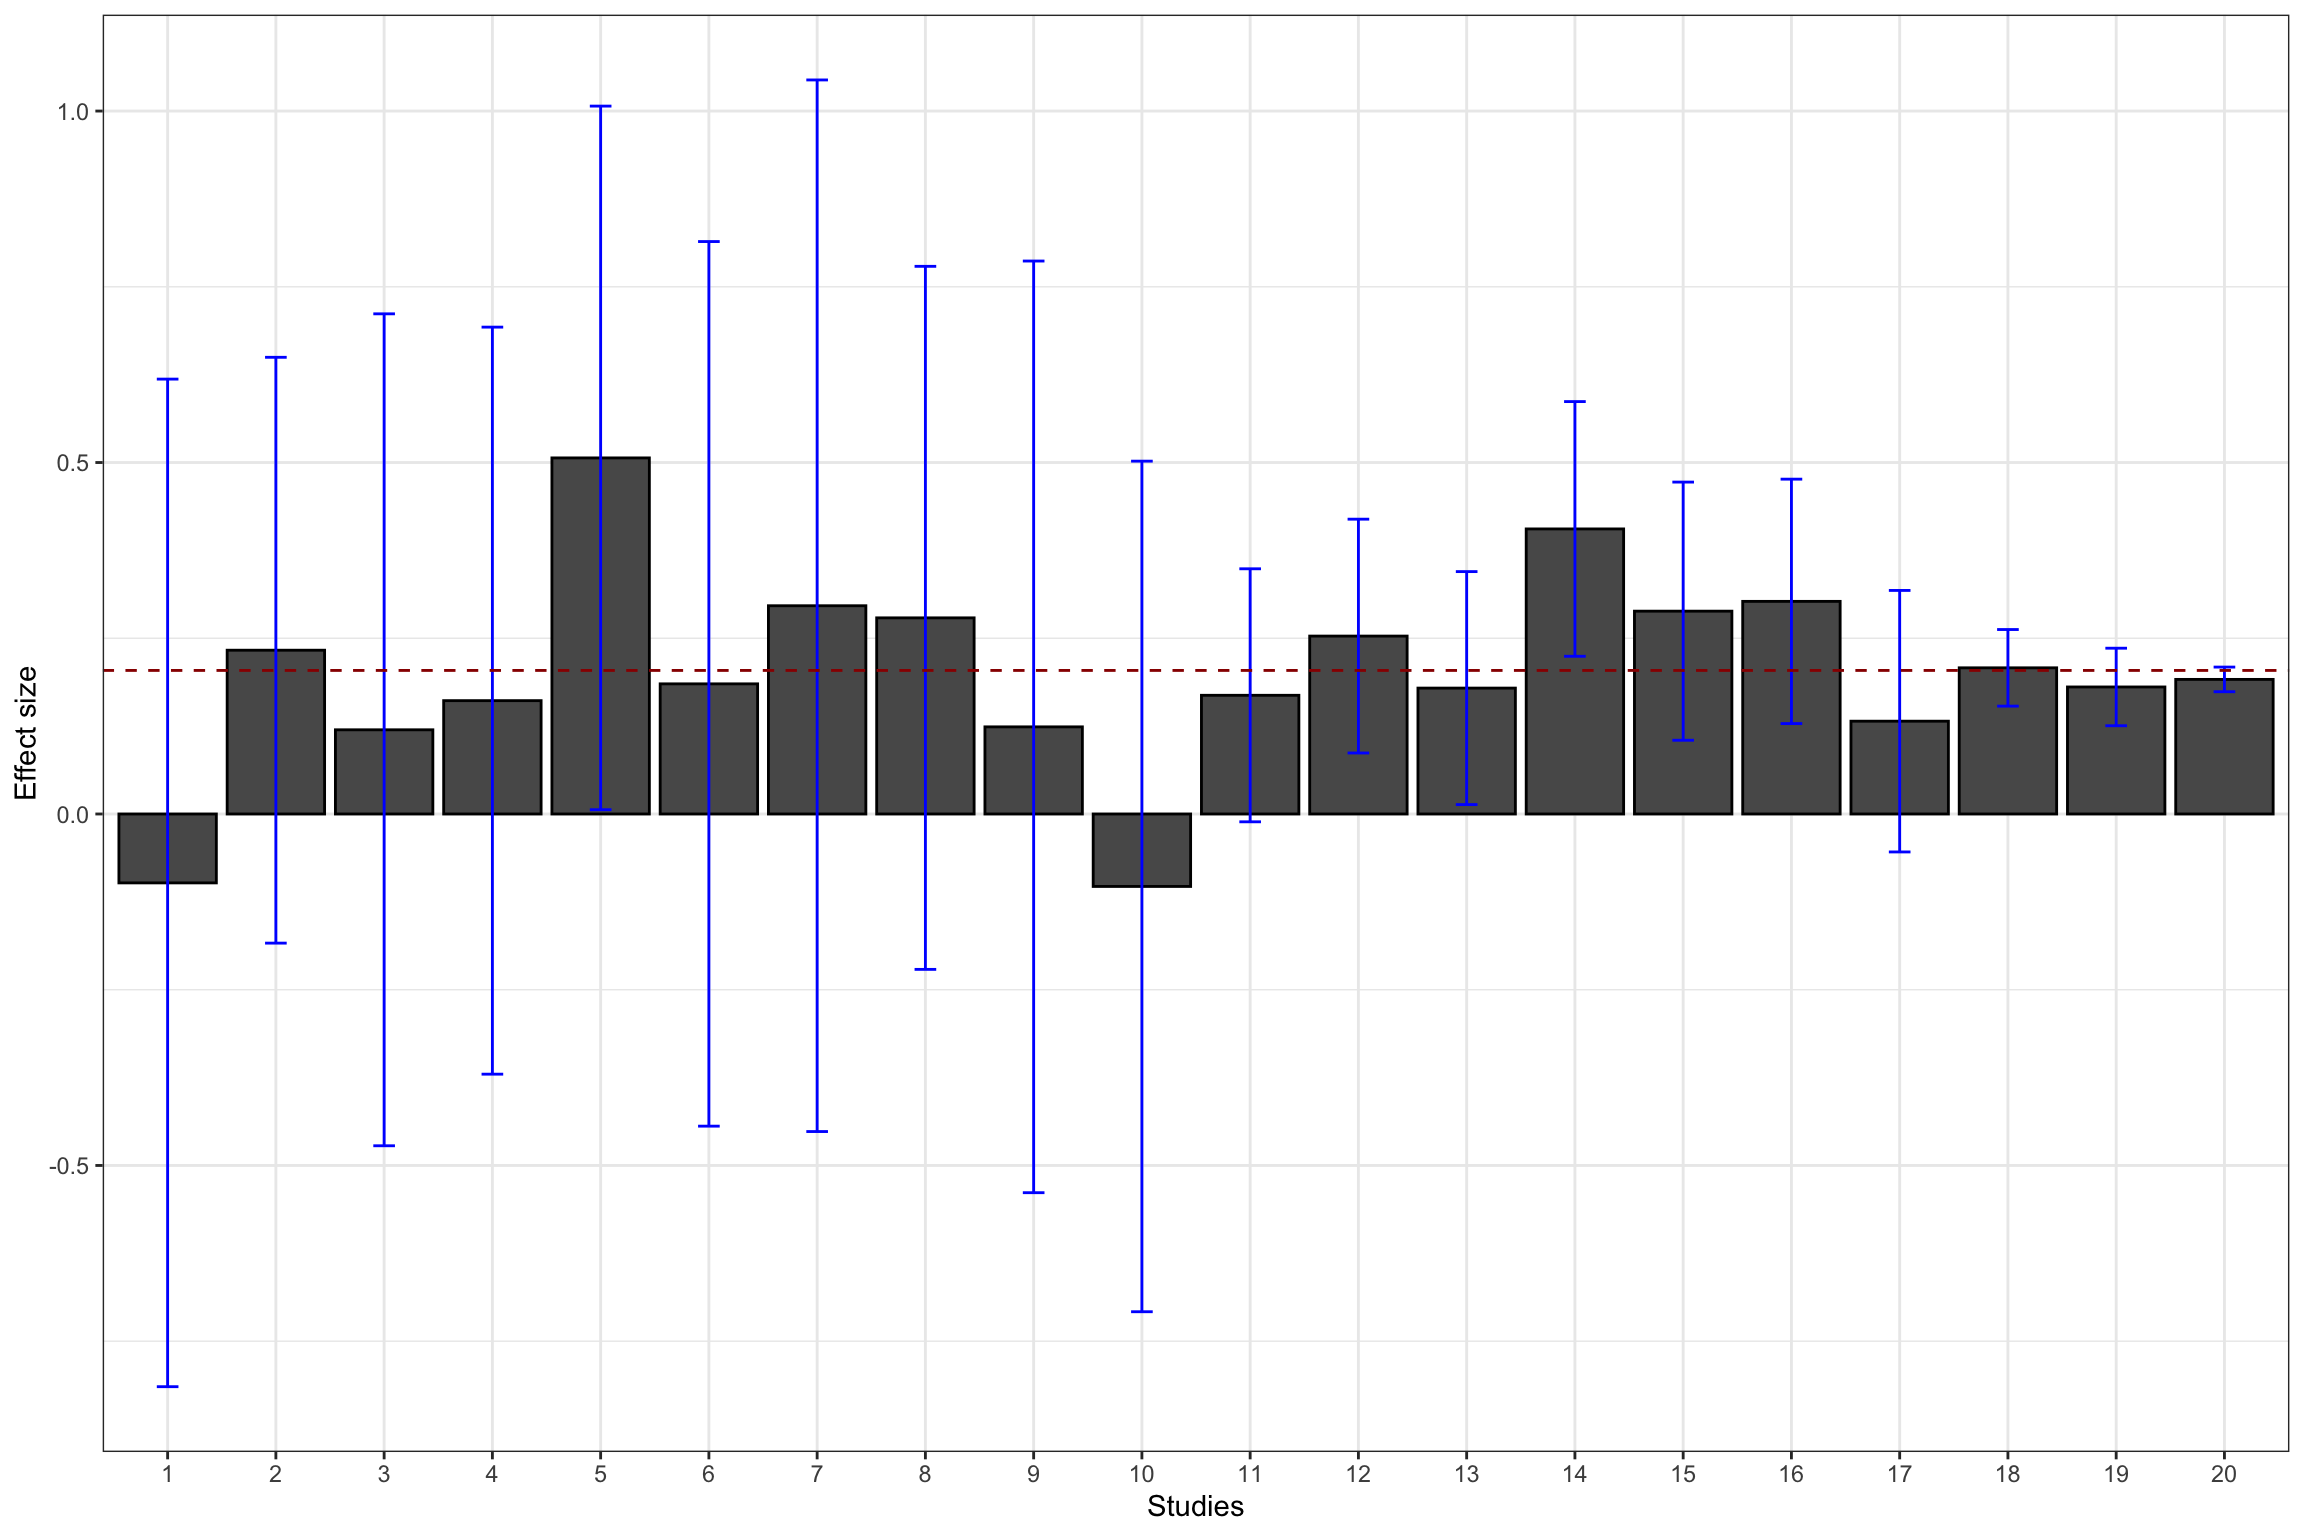
\includegraphics[width=0.6\linewidth]{STCI_files/figure-latex/confintervalESCLT-1} 

}

\caption{Example data set: effect sizes and confidence intervals with $\delta=$ 0.95}\label{fig:confintervalESCLT}
\end{figure}

Figure \ref{fig:confintervalESCLT} shows the resulting sample. I've
selected 10 studies with \(N=\) 100, 7 studies with \(N=\) 1000, 2
studies with \(N=\) 10\^{}\{4\}, and 1 study with \(N=\) 10\^{}\{5\}.
The studies are represented in that order, mimicking the increasing
sample size of studies that accumulate evidence on a treatment, probably
with studies with a small sample size at first, and only large studies
at the end for the most promising treatments.

\subsection{Meta-analysis as a weighted
average}\label{meta-analysis-as-a-weighted-average}

The key idea of meta-analysis is to combine the effect size estimates
stemming from different studies, weighing them by their relative
precision.

\BeginKnitrBlock{definition}[Weighted Meta-Analytic Estimator]
\protect\hypertarget{def:metaweights}{}{\label{def:metaweights}
\iffalse (Weighted Meta-Analytic Estimator) \fi{} }The weighted
meta-analytic estimator is \[
\bar{\theta} = \sum_{k=1}^Nw_k\hat{\theta}_k \text{ with } w_k=\frac{\frac{1}{\hat{\sigma}^2_k}}{\sum_{k=1}^N\frac{1}{\hat{\sigma}^2_k}}.
\]
\EndKnitrBlock{definition}

Under some assumptions, the estimator \(\bar{\theta}\) converges to the
true effect of the treatment. Let's delineate these assumptions.

\BeginKnitrBlock{definition}[Homogeneous Treatment Effect]
\protect\hypertarget{def:metahomo}{}{\label{def:metahomo}
\iffalse (Homogeneous Treatment Effect) \fi{} }Each \(\hat{\theta}_k\)
converges to the same treatment effect \(\theta\).
\EndKnitrBlock{definition}

Assumption \ref{def:metahomo} imposes that all the studies have been
drawn from the same population, where the treatment effect is a
constant.

\BeginKnitrBlock{definition}[Independence of Estimates]
\protect\hypertarget{def:metaind}{}{\label{def:metaind}
\iffalse (Independence of Estimates) \fi{} }The \(\hat{\theta}_k\) are
independent from each other.
\EndKnitrBlock{definition}

Assumption \ref{def:metaind} imposes that all the studies estimates are
independent from each other. That means that they do not share sampling
units and that they are not affected by common shocks.

Under these assumptions, we can show two important results.

\BeginKnitrBlock{theorem}[Consistency of the Weighted Meta-Analytic Estimator]
\protect\hypertarget{thm:metafixedcons}{}{\label{thm:metafixedcons}
\iffalse (Consistency of the Weighted Meta-Analytic Estimator) \fi{}
}Under Assumptions \ref{def:metahomo} and \ref{def:metaind}, when the
sample size of each study goes to infinity,
\(\bar{\theta}\approx\theta\).
\EndKnitrBlock{theorem}

\BeginKnitrBlock{proof}
\iffalse{} {Proof. } \fi{}The Law of Large Number applied to each sample
gives the fact that the estimator is a weighted sum of \(\theta\) with
weights summing to one. Hence the result.
\EndKnitrBlock{proof}

Theorem \ref{thm:metafixedcons} says that the error we are making around
the true effect of the treatment goes to zero as the sample size in each
study decrease. This is great: aggregating the studies is thus going to
get us to the truth.

\BeginKnitrBlock{remark}
\iffalse{} {Remark. } \fi{}One interesting question is whether Theorem
\ref{thm:metafixedcons} also holds when the size of the individual
studies remains fixed and the number of studies goes to infinity, which
seems a more natural way to do asymptotics in a meta-analysis. I'm
pretty sure that is the case. Indeed, the studies constitute an enormous
sample in which we take the average outcomes of the treated on the one
hand and of the untreated on the other. These averages differ from the
usual ones in the Law of Large Numbers only by the fact that the weights
are not equal to one. But they (i) are independent from the outcomes and
(ii) sum to one. As a consequence, I'm pretty sure the Law of Large
Numbers also apply in this dimension.
\EndKnitrBlock{remark}

\textbf{\textsc{Check if this is a consequence of Kolmogorov's Law of
Large Numbers.}}

\BeginKnitrBlock{theorem}[Asymptotic Distribution of the Weighted Meta-Analytic Estimator]
\protect\hypertarget{thm:metafixeddis}{}{\label{thm:metafixeddis}
\iffalse (Asymptotic Distribution of the Weighted Meta-Analytic
Estimator) \fi{} }Under Assumptions \ref{def:metahomo} and
\ref{def:metaind}, when the sample size of each study goes to infinity,
\(\bar{\theta}\stackrel{d}{\rightarrow}\mathcal{N}(\theta,\sigma^2)\),
with \[
\sigma^2 = \frac{1}{\sum_{k=1}^N\frac{1}{\sigma^2_k}}.
\]
\EndKnitrBlock{theorem}

\BeginKnitrBlock{proof}
\iffalse{} {Proof. } \fi{}\textbf{\textsc{To do using the
Lindenberg-Levy version of the Central Limit Theorem.}}
\EndKnitrBlock{proof}

Theorem \ref{thm:metafixeddis} shows that the distribution of the
weighted meta-analytic estimator converges to a normal, which is very
convenient in order to compute sampling noise. In order to obtain an
estimator \(\hat{\sigma}^2\) of the variance of the meta-analytic
estimator, we can simply replace the individual variance terms by their
estimates: \(\hat{\sigma}_k^2\).

\BeginKnitrBlock{remark}
\iffalse{} {Remark. } \fi{}I've taken Theorem \ref{thm:metafixeddis}
from Hedges and Olkin, but I think it is much more interesting and
correct when the asymptotics goes in the number of studies.
\EndKnitrBlock{remark}

\BeginKnitrBlock{remark}
\iffalse{} {Remark. } \fi{}According to Hedges and Olkin, the weighted
meta-analytic estimator is the most efficient estimator available.
\EndKnitrBlock{remark}

\begin{Shaded}
\begin{Highlighting}[]
\NormalTok{wmae <-}\StringTok{ }\ControlFlowTok{function}\NormalTok{(theta,sigma2)\{}
  \KeywordTok{return}\NormalTok{(}\KeywordTok{c}\NormalTok{(}\KeywordTok{weighted.mean}\NormalTok{(theta,(}\DecValTok{1}\OperatorTok{/}\NormalTok{sigma2)}\OperatorTok{/}\NormalTok{(}\KeywordTok{sum}\NormalTok{(}\DecValTok{1}\OperatorTok{/}\NormalTok{sigma2))),}\DecValTok{1}\OperatorTok{/}\KeywordTok{sum}\NormalTok{(}\DecValTok{1}\OperatorTok{/}\NormalTok{sigma2)))}
\NormalTok{\}}
\end{Highlighting}
\end{Shaded}

\BeginKnitrBlock{example}
\protect\hypertarget{exm:unnamed-chunk-128}{}{\label{exm:unnamed-chunk-128}
}Let's use our meta-analytic estimator to estimate the effect size of
our treatment.
\EndKnitrBlock{example} The estimated treatment effect size with our
sample is 0.19 \(\pm\) 0.02. A very simple way to implement such an
estimator in R is to use the \texttt{rma} command of the
\texttt{metafor} package.

\begin{Shaded}
\begin{Highlighting}[]
\NormalTok{data.meta}\OperatorTok{$}\NormalTok{var.ES <-}\StringTok{ }\NormalTok{data.meta}\OperatorTok{$}\NormalTok{se.ES}\OperatorTok{^}\DecValTok{2}
\NormalTok{meta.example.FE <-}\StringTok{ }\KeywordTok{rma}\NormalTok{(}\DataTypeTok{yi =}\NormalTok{ data.meta}\OperatorTok{$}\NormalTok{ES,}\DataTypeTok{vi=}\NormalTok{data.meta}\OperatorTok{$}\NormalTok{var.ES,}\DataTypeTok{method=}\StringTok{"FE"}\NormalTok{)}
\KeywordTok{summary}\NormalTok{(meta.example.FE)}
\end{Highlighting}
\end{Shaded}

\begin{verbatim}
## 
## Fixed-Effects Model (k = 20)
## 
##   logLik  deviance       AIC       BIC      AICc  
##  16.1375   12.7060  -30.2751  -29.2793  -30.0529  
## 
## Test for Heterogeneity: 
## Q(df = 19) = 12.7060, p-val = 0.8533
## 
## Model Results:
## 
## estimate      se     zval    pval   ci.lb   ci.ub     
##   0.1950  0.0079  24.6975  <.0001  0.1795  0.2104  ***
## 
## ---
## Signif. codes:  0 '***' 0.001 '**' 0.01 '*' 0.05 '.' 0.1 ' ' 1
\end{verbatim}

As seen above, the \texttt{metafor} package yields a meta-analytic
estimate of 0.19 \(\pm\) 0.02, as we have found using the weighted
meta-analytic estimator.

It is customary to present the results of a meta-analysis using a forest
plot. A forest plows all the individual estimates along with the
aggregated estimate. Figure \ref{fig:FEforestplot} presents the forest
plot for our example using the very convenient \texttt{forest} function
in the \texttt{metafor} package:

\begin{Shaded}
\begin{Highlighting}[]
\KeywordTok{forest}\NormalTok{(meta.example.FE,}\DataTypeTok{slab =} \KeywordTok{paste}\NormalTok{(}\StringTok{'Study'}\NormalTok{,data.meta}\OperatorTok{$}\NormalTok{id,}\DataTypeTok{sep=}\StringTok{' '}\NormalTok{),}\DataTypeTok{xlab=}\StringTok{'Estimated Meta-analytic Parameter'}\NormalTok{)}
\end{Highlighting}
\end{Shaded}

\begin{figure}[htbp]

{\centering 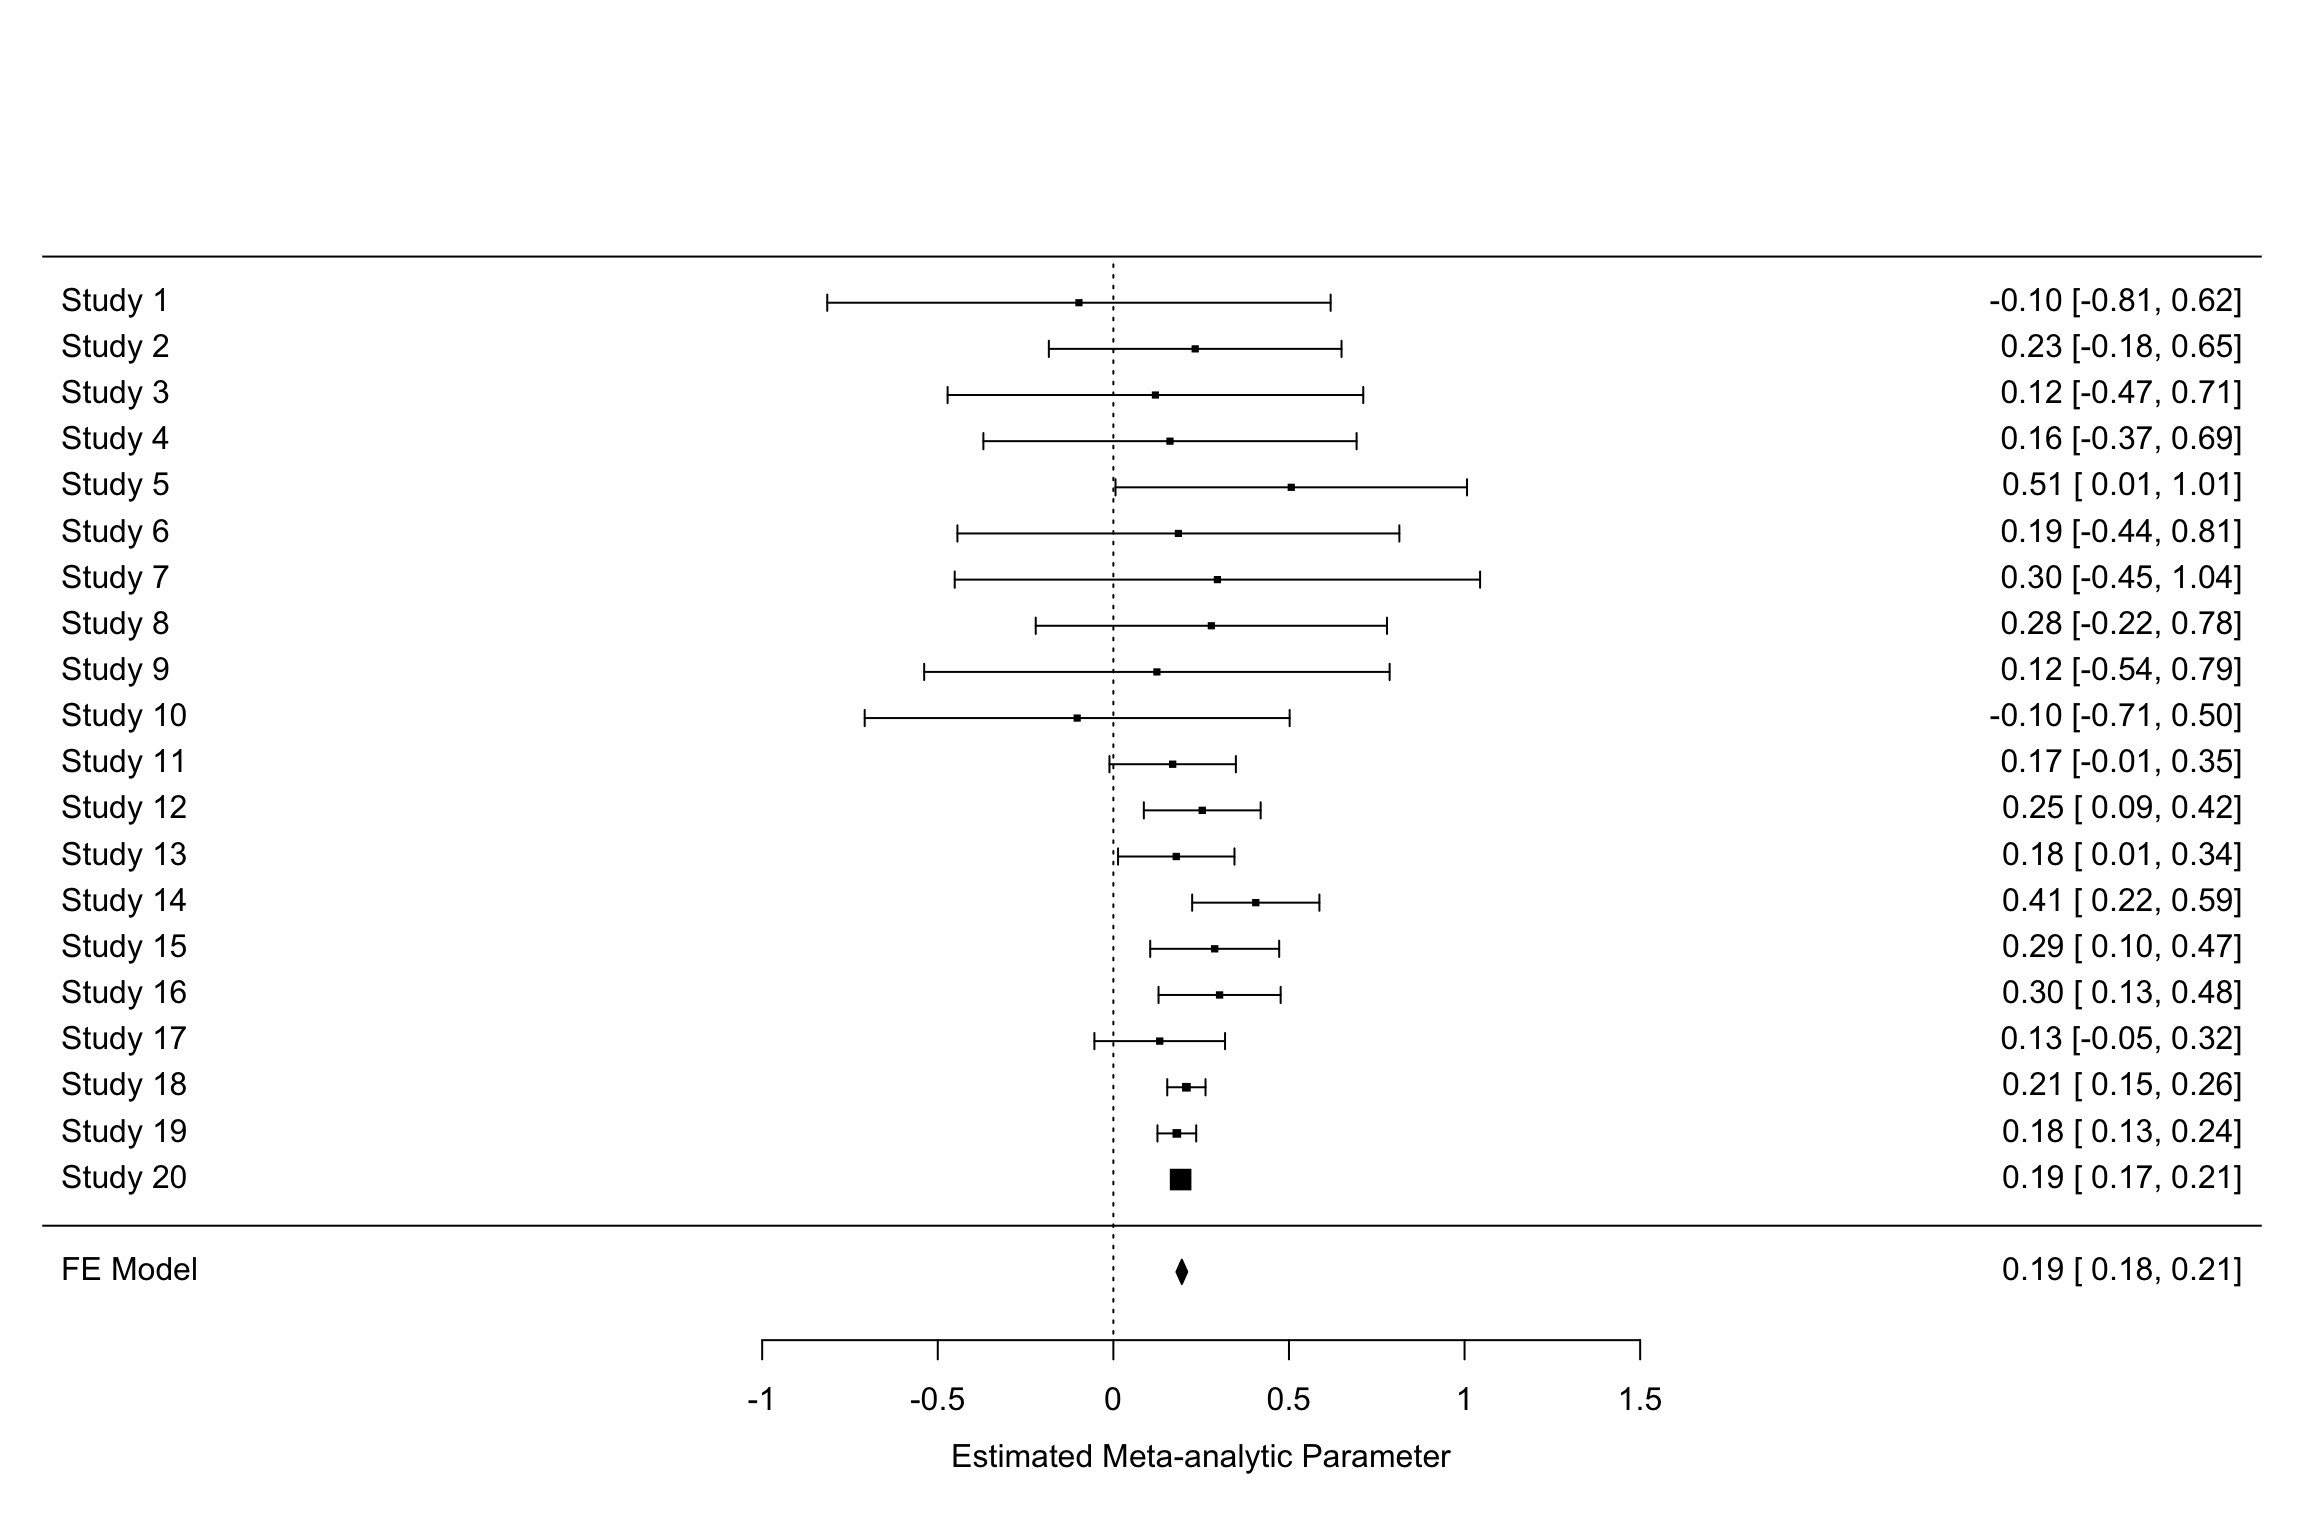
\includegraphics[width=0.6\linewidth]{STCI_files/figure-latex/FEforestplot-1} 

}

\caption{Example data set: forest plot}\label{fig:FEforestplot}
\end{figure}

\subsection{Constantly updated
meta-analysis}\label{constantly-updated-meta-analysis}

Constantly updated meta-analysis performs the meta-analysis in a
progressive manner, as the results keep arriving. This is a very
important tool that enables us to aggregate constantly the information
coming from different studies. Moreover, restrospectively, it helps us
to assess when we would have reached enough precision so that we could
have foregone an additional study. The way constantly updated
meta-analysis works is simply by performing a new meta-analysis each
time a new results pops up.

\BeginKnitrBlock{example}
\protect\hypertarget{exm:unnamed-chunk-129}{}{\label{exm:unnamed-chunk-129}
}Figure \ref{fig:cumWMAE} shows how constantly updated meta-analysis
works in our example.
\EndKnitrBlock{example}

\begin{Shaded}
\begin{Highlighting}[]
\NormalTok{cum.wmae.}\DecValTok{1}\NormalTok{ <-}\StringTok{ }\ControlFlowTok{function}\NormalTok{(k,theta,sigma2)\{}
  \KeywordTok{return}\NormalTok{(}\KeywordTok{c}\NormalTok{(}\KeywordTok{weighted.mean}\NormalTok{(theta[}\DecValTok{1}\OperatorTok{:}\NormalTok{k],(}\DecValTok{1}\OperatorTok{/}\NormalTok{sigma2[}\DecValTok{1}\OperatorTok{:}\NormalTok{k])}\OperatorTok{/}\NormalTok{(}\KeywordTok{sum}\NormalTok{(}\DecValTok{1}\OperatorTok{/}\NormalTok{sigma2[}\DecValTok{1}\OperatorTok{:}\NormalTok{k]))),}\DecValTok{1}\OperatorTok{/}\KeywordTok{sum}\NormalTok{(}\DecValTok{1}\OperatorTok{/}\NormalTok{sigma2[}\DecValTok{1}\OperatorTok{:}\NormalTok{k])))}
\NormalTok{\}}

\NormalTok{cum.wmae <-}\StringTok{ }\ControlFlowTok{function}\NormalTok{(theta,sigma2)\{}
  \KeywordTok{return}\NormalTok{(}\KeywordTok{sapply}\NormalTok{(}\DecValTok{1}\OperatorTok{:}\KeywordTok{length}\NormalTok{(theta),cum.wmae.}\DecValTok{1}\NormalTok{,}\DataTypeTok{theta=}\NormalTok{theta,}\DataTypeTok{sigma2=}\NormalTok{sigma2))}
\NormalTok{\}}

\NormalTok{cum.test <-}\StringTok{ }\KeywordTok{as.data.frame}\NormalTok{(}\KeywordTok{t}\NormalTok{(}\KeywordTok{cum.wmae}\NormalTok{(data.meta}\OperatorTok{$}\NormalTok{ES,data.meta}\OperatorTok{$}\NormalTok{se.ES}\OperatorTok{^}\DecValTok{2}\NormalTok{)))}
\KeywordTok{colnames}\NormalTok{(cum.test) <-}\StringTok{ }\KeywordTok{c}\NormalTok{(}\StringTok{'cum.ES'}\NormalTok{,}\StringTok{'cum.var'}\NormalTok{)}
\NormalTok{cum.test}\OperatorTok{$}\NormalTok{id <-}\StringTok{ }\DecValTok{1}\OperatorTok{:}\KeywordTok{nrow}\NormalTok{(cum.test)}
\NormalTok{cum.test}\OperatorTok{$}\NormalTok{cum.se.ES <-}\StringTok{ }\KeywordTok{sqrt}\NormalTok{(cum.test}\OperatorTok{$}\NormalTok{cum.var)}

  \KeywordTok{ggplot}\NormalTok{(data.meta, }\KeywordTok{aes}\NormalTok{(}\DataTypeTok{x=}\NormalTok{forcats}\OperatorTok{::}\KeywordTok{fct_rev}\NormalTok{(}\KeywordTok{as.factor}\NormalTok{(id)), }\DataTypeTok{y=}\NormalTok{ES)) }\OperatorTok{+}
\StringTok{      }\KeywordTok{geom_bar}\NormalTok{(}\DataTypeTok{position=}\KeywordTok{position_dodge}\NormalTok{(), }\DataTypeTok{stat=}\StringTok{"identity"}\NormalTok{, }\DataTypeTok{colour=}\StringTok{'black'}\NormalTok{) }\OperatorTok{+}
\StringTok{      }\KeywordTok{geom_errorbar}\NormalTok{(}\KeywordTok{aes}\NormalTok{(}\DataTypeTok{ymin=}\NormalTok{ES}\OperatorTok{-}\KeywordTok{qnorm}\NormalTok{((delta.}\DecValTok{2}\OperatorTok{+}\DecValTok{1}\NormalTok{)}\OperatorTok{/}\DecValTok{2}\NormalTok{)}\OperatorTok{*}\NormalTok{se.ES, }\DataTypeTok{ymax=}\NormalTok{ES}\OperatorTok{+}\KeywordTok{qnorm}\NormalTok{((delta.}\DecValTok{2}\OperatorTok{+}\DecValTok{1}\NormalTok{)}\OperatorTok{/}\DecValTok{2}\NormalTok{)}\OperatorTok{*}\NormalTok{se.ES), }\DataTypeTok{width=}\NormalTok{.}\DecValTok{2}\NormalTok{,}\DataTypeTok{position=}\KeywordTok{position_dodge}\NormalTok{(.}\DecValTok{9}\NormalTok{),}\DataTypeTok{color=}\StringTok{'blue'}\NormalTok{) }\OperatorTok{+}
\StringTok{      }\KeywordTok{geom_hline}\NormalTok{(}\KeywordTok{aes}\NormalTok{(}\DataTypeTok{yintercept=}\KeywordTok{ES}\NormalTok{(param)), }\DataTypeTok{colour=}\StringTok{"#990000"}\NormalTok{, }\DataTypeTok{linetype=}\StringTok{"dashed"}\NormalTok{)}\OperatorTok{+}
\StringTok{      }\KeywordTok{xlab}\NormalTok{(}\StringTok{"Studies"}\NormalTok{)}\OperatorTok{+}
\StringTok{      }\KeywordTok{ylab}\NormalTok{(}\StringTok{"Initial effect size"}\NormalTok{)}\OperatorTok{+}
\StringTok{      }\KeywordTok{theme_bw}\NormalTok{()}\OperatorTok{+}
\StringTok{      }\KeywordTok{coord_flip}\NormalTok{()}

  \KeywordTok{ggplot}\NormalTok{(cum.test, }\KeywordTok{aes}\NormalTok{(}\DataTypeTok{x=}\NormalTok{forcats}\OperatorTok{::}\KeywordTok{fct_rev}\NormalTok{(}\KeywordTok{as.factor}\NormalTok{(id)), }\DataTypeTok{y=}\NormalTok{cum.ES)) }\OperatorTok{+}
\StringTok{      }\KeywordTok{geom_bar}\NormalTok{(}\DataTypeTok{position=}\KeywordTok{position_dodge}\NormalTok{(), }\DataTypeTok{stat=}\StringTok{"identity"}\NormalTok{, }\DataTypeTok{colour=}\StringTok{'black'}\NormalTok{) }\OperatorTok{+}
\StringTok{      }\KeywordTok{geom_errorbar}\NormalTok{(}\KeywordTok{aes}\NormalTok{(}\DataTypeTok{ymin=}\NormalTok{cum.ES}\OperatorTok{-}\KeywordTok{qnorm}\NormalTok{((delta.}\DecValTok{2}\OperatorTok{+}\DecValTok{1}\NormalTok{)}\OperatorTok{/}\DecValTok{2}\NormalTok{)}\OperatorTok{*}\NormalTok{cum.se.ES, }\DataTypeTok{ymax=}\NormalTok{cum.ES}\OperatorTok{+}\KeywordTok{qnorm}\NormalTok{((delta.}\DecValTok{2}\OperatorTok{+}\DecValTok{1}\NormalTok{)}\OperatorTok{/}\DecValTok{2}\NormalTok{)}\OperatorTok{*}\NormalTok{cum.se.ES), }\DataTypeTok{width=}\NormalTok{.}\DecValTok{2}\NormalTok{,}\DataTypeTok{position=}\KeywordTok{position_dodge}\NormalTok{(.}\DecValTok{9}\NormalTok{),}\DataTypeTok{color=}\StringTok{'blue'}\NormalTok{) }\OperatorTok{+}
\StringTok{      }\KeywordTok{geom_hline}\NormalTok{(}\KeywordTok{aes}\NormalTok{(}\DataTypeTok{yintercept=}\KeywordTok{ES}\NormalTok{(param)), }\DataTypeTok{colour=}\StringTok{"#990000"}\NormalTok{, }\DataTypeTok{linetype=}\StringTok{"dashed"}\NormalTok{)}\OperatorTok{+}
\StringTok{      }\KeywordTok{xlab}\NormalTok{(}\StringTok{"Studies"}\NormalTok{)}\OperatorTok{+}
\StringTok{      }\KeywordTok{ylab}\NormalTok{(}\StringTok{"Cumulative effect size"}\NormalTok{)}\OperatorTok{+}
\StringTok{      }\KeywordTok{theme_bw}\NormalTok{()}\OperatorTok{+}
\StringTok{      }\KeywordTok{coord_flip}\NormalTok{()}
\end{Highlighting}
\end{Shaded}

\begin{figure}[htbp]

{\centering \subfloat[Initial data set\label{fig:cumWMAE1}]{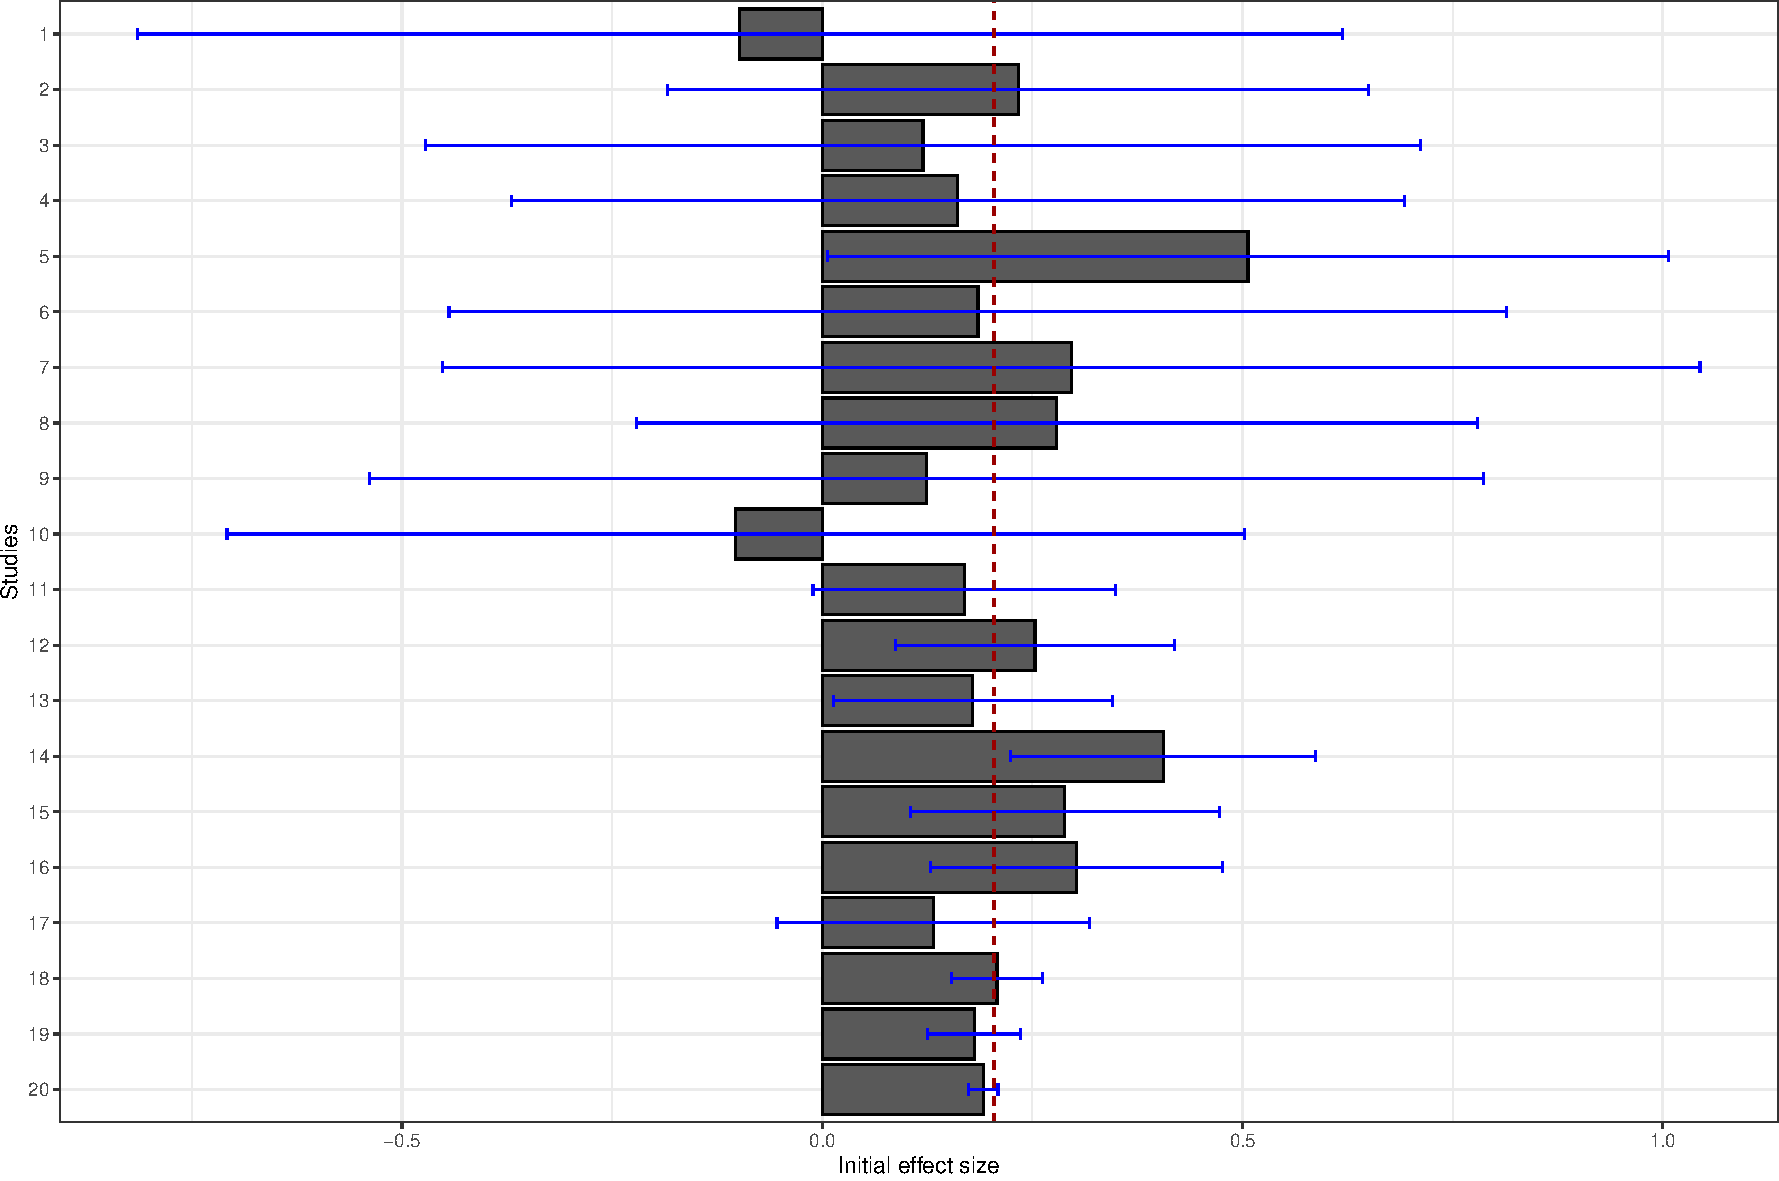
\includegraphics[width=0.5\linewidth]{STCI_files/figure-latex/cumWMAE-1} }\subfloat[Constantly updated dataset\label{fig:cumWMAE2}]{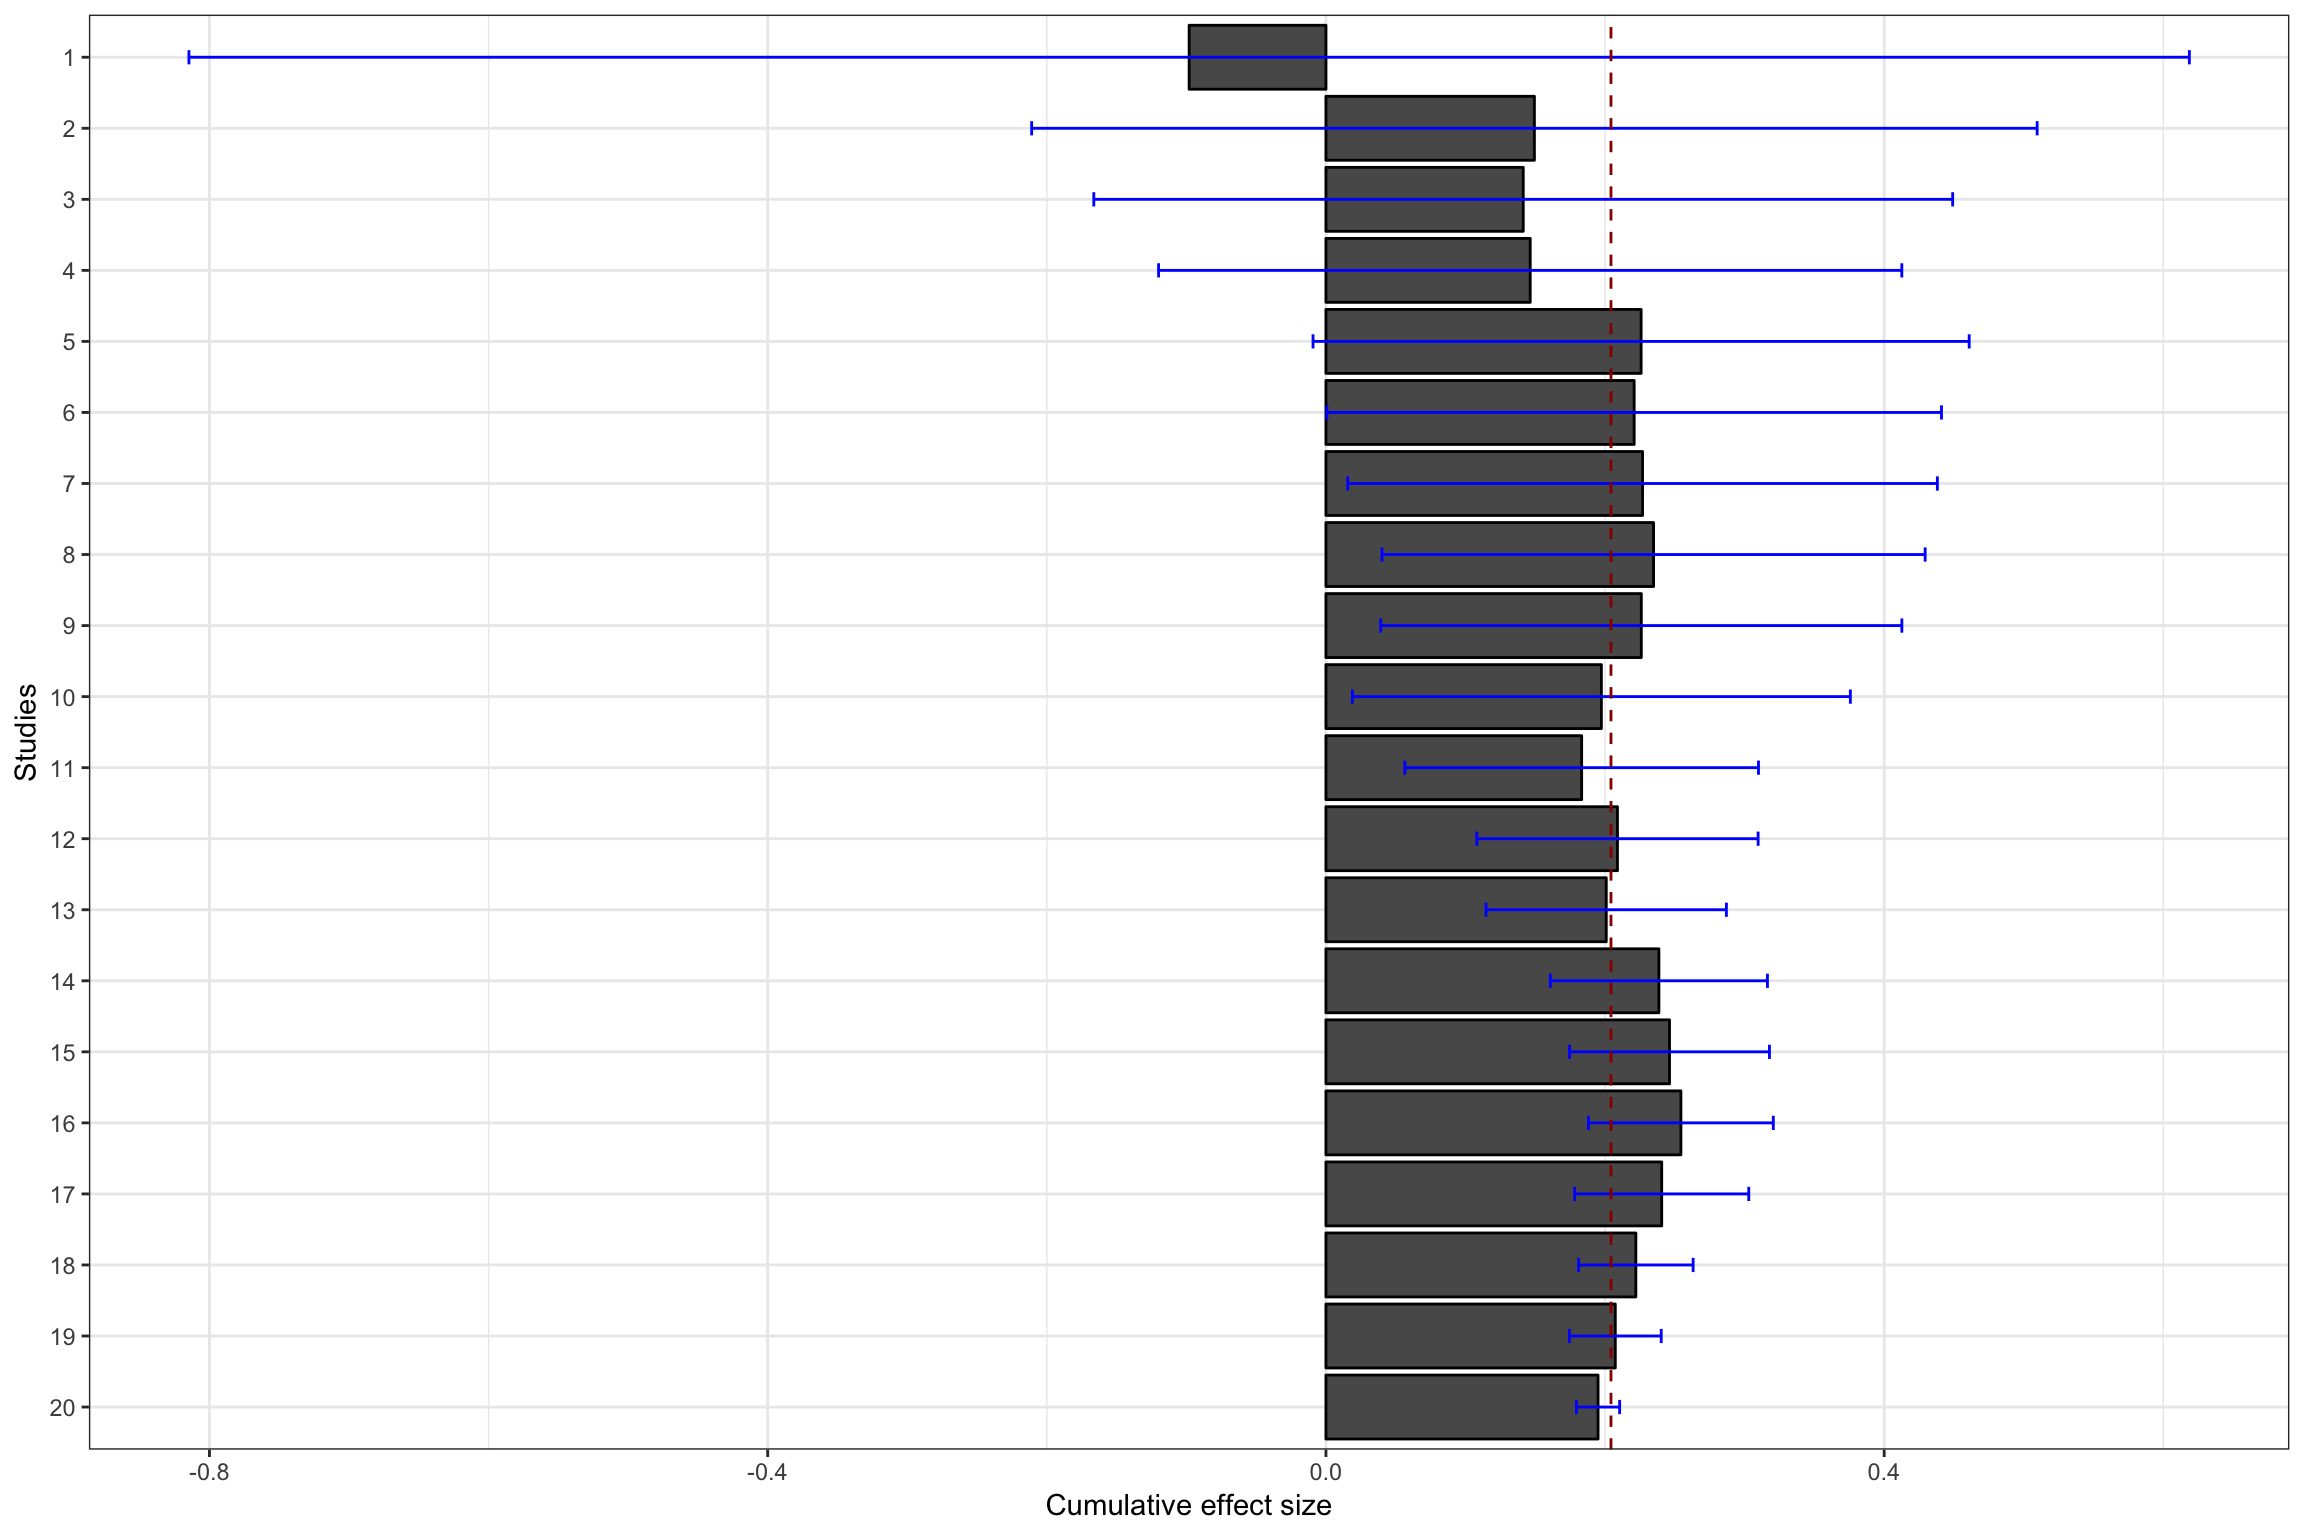
\includegraphics[width=0.5\linewidth]{STCI_files/figure-latex/cumWMAE-2} }

}

\caption{Constantly updated meta-analysis}\label{fig:cumWMAE}
\end{figure}

Figure \ref{fig:cumWMAE} shows that combining several imprecise
estimates might help you reach the same precision as running a larger
experiment.\\
For instance, cumulating the first 10 studies with a small sample size
(\(N=\) 100), the meta-analytic effect is estimated at 0.2 \(\pm\) 0.18.
This is very close to the individual estimate obtained from the first
estimate with a larger sample size (sample 11 on Figure
\ref{fig:cumWMAE}, with \(N=\) 1000): 0.17 \(\pm\) 0.18. Both estimates
actually have the exact same precision (because they actually have the
same sample size). The same is true when combining the first 17 studies.
The meta-analytic effect is estimated at 0.24 \(\pm\) 0.06, while the
effect estimated using one unique RCT with a larger sample size (sample
18 on Figure \ref{fig:cumWMAE}, with \(N=\) 10\^{}\{4\}) is 0.21 \(\pm\)
0.05. Finally, the same result occurs when combining the first 19
studies. The meta-analytic effect is estimated at 0.21 \(\pm\) 0.03,
while the effect estimated using one unique RCT with a larger sample
size (sample 20 on Figure \ref{fig:cumWMAE}, with \(N=\) 10\^{}\{5\}) is
0.19 \(\pm\) 0.02.

As a conclusion, constantly updated meta-analysis would have each time
delivered the same result than the one found with a much larger study,
rendering this additional study almost irrelevant. This is a very
important result: beyond the apparent messiness of the first noisy
estimates in Figures \ref{fig:confintervalESCLT} and
\ref{fig:FEforestplot} lies an order that can be retrieved and made
apparent using constantly updated meta-analysis. Sometimes, the answer
is right there in front of our eyes, we just lack the ability to see it.
Constantly updated meta-analysis serves as a binocular to magnify what
is there. Think about how costly it woud be to run a very large study,
just to find out that the we did not really need it because we had known
the result all along.

\BeginKnitrBlock{remark}
\iffalse{} {Remark. } \fi{}Something pretty cool is that I can reproduce
Figure \ref{fig:cumWMAE} using the \texttt{metafor} package with much
less lines of code.
\EndKnitrBlock{remark}

\begin{Shaded}
\begin{Highlighting}[]
\KeywordTok{forest}\NormalTok{(meta.example.FE,}\DataTypeTok{slab =} \KeywordTok{paste}\NormalTok{(}\StringTok{'Study'}\NormalTok{,data.meta}\OperatorTok{$}\NormalTok{id,}\DataTypeTok{sep=}\StringTok{' '}\NormalTok{),}\DataTypeTok{xlab=}\StringTok{'Estimated Meta-analytic Parameter'}\NormalTok{)}
\NormalTok{cumul.meta.example.FE <-}\StringTok{ }\KeywordTok{cumul}\NormalTok{(meta.example.FE, }\DataTypeTok{order=}\NormalTok{data.meta}\OperatorTok{$}\NormalTok{id)}
\KeywordTok{forest}\NormalTok{(cumul.meta.example.FE,}\DataTypeTok{slab =} \KeywordTok{paste}\NormalTok{(}\StringTok{'Study'}\NormalTok{,data.meta}\OperatorTok{$}\NormalTok{id,}\DataTypeTok{sep=}\StringTok{' '}\NormalTok{),}\DataTypeTok{xlab=}\StringTok{'Estimated Meta-analytic Cumulated Parameter'}\NormalTok{)}
\end{Highlighting}
\end{Shaded}

\begin{figure}[htbp]

{\centering \subfloat[Initial data set\label{fig:cumWMAEmetafor1}]{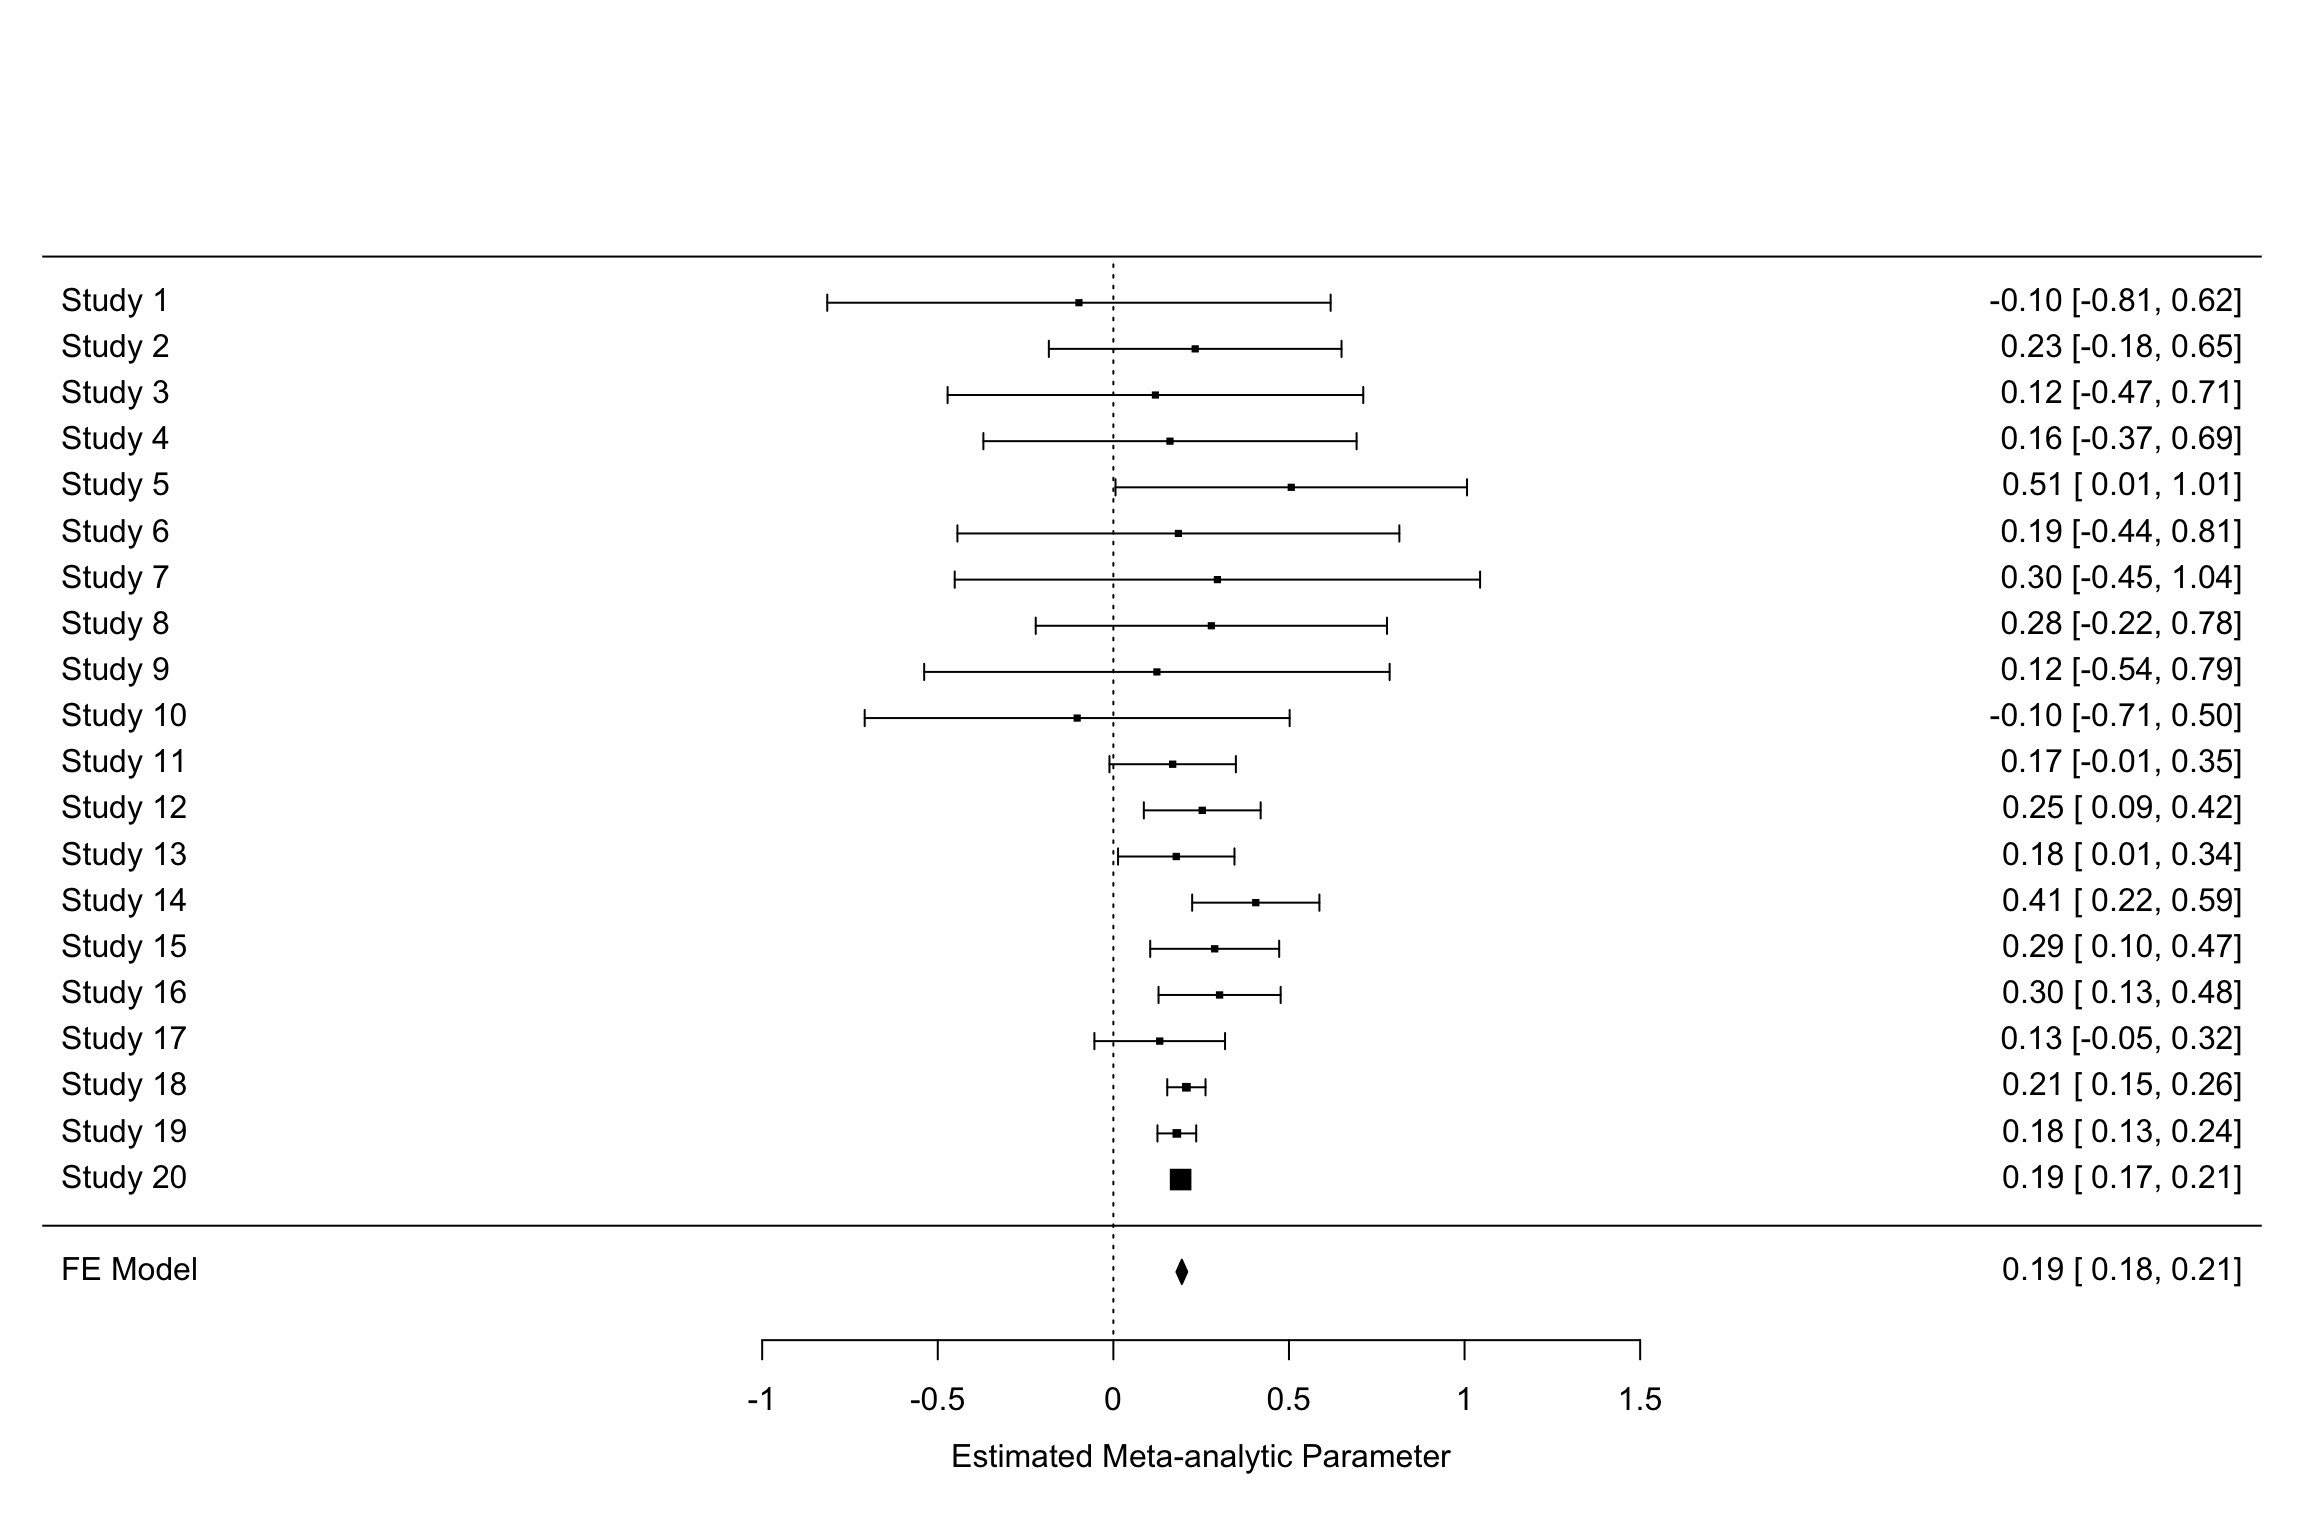
\includegraphics[width=0.5\linewidth]{STCI_files/figure-latex/cumWMAEmetafor-1} }\subfloat[Constantly updated dataset\label{fig:cumWMAEmetafor2}]{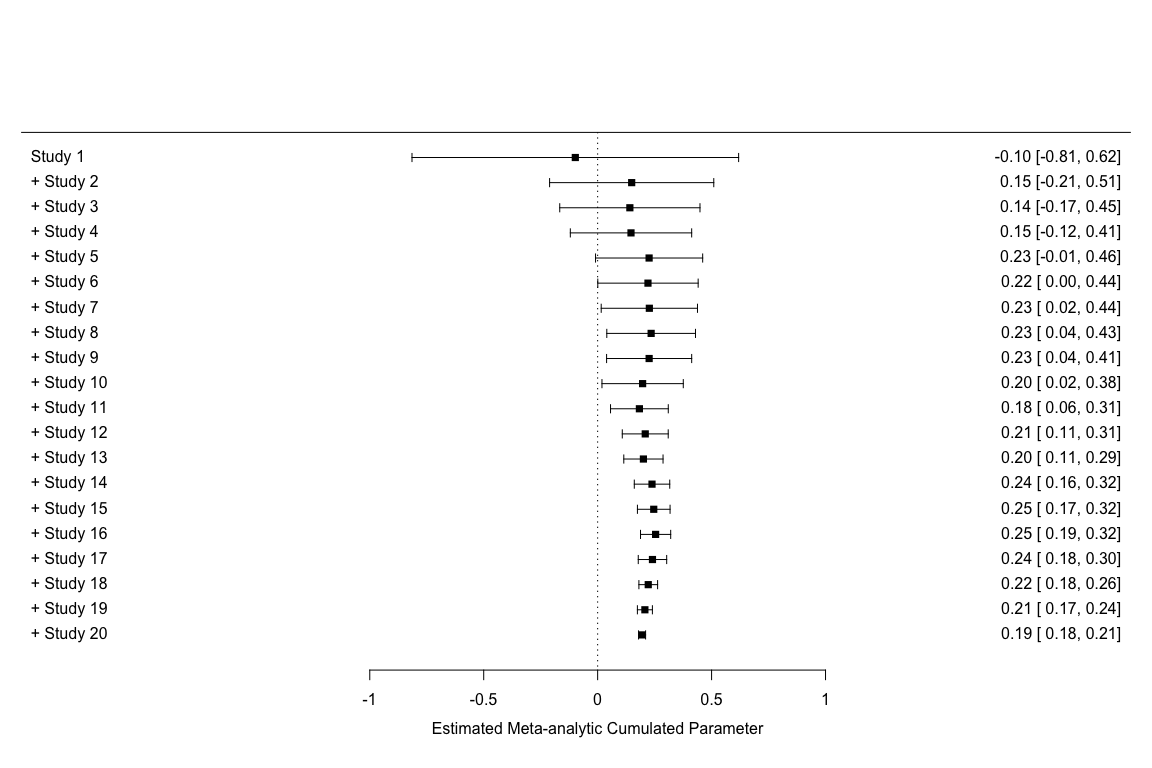
\includegraphics[width=0.5\linewidth]{STCI_files/figure-latex/cumWMAEmetafor-2} }

}

\caption{Constantly updated meta-analysis with the `metafor` package}\label{fig:cumWMAEmetafor}
\end{figure}

You can also call each of the individual results of the cumulative
meta-analysis using \texttt{cumul.meta.example.FE\$estimate}. For
example, the cumulated effect size after the 10 first studies is equal
to 0.2 \(\pm\) 0.18.

\subsection{Testing for the homogeneity of treatment
effects}\label{testing-for-the-homogeneity-of-treatment-effects}

One key assumption that we have just made so far is that of homogeneous
treatment effect. We have worked under the assumption that each study
was drawn from the same population, where the treatment effect is a
constant. Why would the treatment effects differ in each study?

\begin{enumerate}
\def\labelenumi{\arabic{enumi}.}
\tightlist
\item
  We do not study exactly the same treatment, but a family of similar
  treatments. Each individual study covers a particular iteration of the
  treatment, each with its idiosyncratic parameterization. The
  particular value of the transfer in a Cash Transfer program, or of the
  conditions to receive it, or the length of payment, whether it is in
  one time or over some period, might make a difference, for example.
  The same is true for Job Training Programs, Payments for Environmental
  Services, microcredit, graduation programs, nudges, etc. Actually,
  most programs that economists study differ from one implementation to
  the next. In psychology and medecine, most treatments are accompanied
  by a rigorous protocol that makes them much more homogeneous.
\item
  The population on which the treatment is applied varies. For example,
  similar Job Training Programs or microcredit initiatives might have
  very different outcomes depending on the business cycle. Education
  interventions might have very different effects depending on the
  background of the students on which they are tested. A drug might
  interact with patients' phenotype and genotype to generate different
  effects, and the populations from which the experimental samples are
  drawn do not have to be similar. As an extreme example, think of a
  vaccine tested in a population where the prevalence of a disease is
  null. The treatment effect is zero. Now, test the vaccine in a
  population where the disease is endemic: the treatment effect might be
  huge.
\end{enumerate}

We can also think that the treatment effect differs in each sample
because the composition of the sample changes. But this is normal
variation due to sampling noise and is to be expected. It is not the
same thing as assuming that the population effect differs.

What can we do in order to test whether there is heterogeneity in
treatment effects? One way is to build an index comparing the usual
variation in treatment effects stemming from sampling noise to the one
stemming from variation between studies. If we find that the variation
between studies dwarves the variation due to sampling noise in each
study, then there is some heterogeneity for sure. One statistics that
does that is the \(Q\) statistic where the variation in treatment
effects between studies is estimated using the difference between the
individual effect size and the average one squared:

\begin{align*}
  Q & = \sum_{k=1}^N\frac{(\hat{\theta}_k-\bar{\theta})^2}{\hat{\sigma}^2_k}.
\end{align*}

What is great with the \(Q\) statistic is that, under the Null
hypothesis that all the treatment effects are equal to the same
constant, it is distributed asymptotically as a \(\chi^2\) distribution
with \(N-1\) degrees of freedom, and thus it can directly be used to
test for the hypothesis of homogeneous treatment effects.

\BeginKnitrBlock{example}
\protect\hypertarget{exm:unnamed-chunk-131}{}{\label{exm:unnamed-chunk-131}
}In our example, we have already computed the \(Q\) statistic when we
have used the \texttt{rma} function in the \texttt{metafor} package. In
order to access it, we just need to extract it using
\texttt{meta.example.FE\$QE} for the \(Q\) statistic and
\texttt{meta.example.FE\$QEp} for its p-value.
\EndKnitrBlock{example} The \(Q\) statistic in our example has value
12.71, with associated p-value 0.85. We end up not rejecting
homogeneity, which is correct.

\BeginKnitrBlock{remark}
\iffalse{} {Remark. } \fi{}The problem with using test statistics for
testing for treatment effect homogeneity is that, when precision
increases, we might end up rejecting homogeneity despite the fact that
it is there.
\EndKnitrBlock{remark}

\textbf{\textsc{Test with \(N=10^5\).}}

\BeginKnitrBlock{remark}
\iffalse{} {Remark. } \fi{}The \(\chi^2\) distribution with \(k\)
degrees of freedom is asymptotically distributed as a normal with mean
\(k\) and variance \(2k\). So, when \(k\) is large, a good rule of thumb
for assessing the homogeneity of the treatment effect estimates is to
compare the \(Q\) statistic to the number of studies. If it is much
larger, homogeneity is probably not guaranteed.
\EndKnitrBlock{remark}

\subsection{Meta-analysis when treatment effects are
heterogeneous}\label{meta-analysis-when-treatment-effects-are-heterogeneous}

When each study draws a treatment effect from a distinct population,
meta-analysis has to take into account that treatment effects are
heterogeneous. The main consequence of treatment effect heterogeneity is
that the weighting approach we have used so far underestimates the
uncertainty around the true effect, since it does not acknowledge that
there is additional variation within each study.

There are two main ways to account for heterogeneity in meta-analysis:

\begin{enumerate}
\def\labelenumi{\arabic{enumi}.}
\tightlist
\item
  \textbf{Meta-regression} trying to capture the heterogeneity in
  treatment effects with observed covariates.
\item
  \textbf{Random effects} allowing for additional random noise in each
  study.
\end{enumerate}

In this section, we are going to study the random effects approach, and
we'll defer the meta-regression for the next section.

\subsubsection{Estimating the variance of the treatment effect across
sites}\label{estimating-the-variance-of-the-treatment-effect-across-sites}

The key component of the random effects approach is the estimation of
the size of the variance of the treatment effect in the population.
Indeed, the observed effect size estimate for a given study \(k\) is
modelled as follows in the random effects approach:

\begin{align*}
\hat{\theta}_k & = \alpha + \epsilon_k + \nu_k,
\end{align*}

where \(\epsilon_k\) is due to sampling noise and \(\nu_k\) is due to
the heterogeneity in effect sizes across sites, while \(\alpha\) is the
average of the effect size accross all populations. We denote the
variance of \(\nu_k\) as \(\tau^2\).

Since Hedges, \(\tau^2\) is estimated as the residual variance in effect
sizes that is not explained by sampling noise. In order to compute this
estimator, first estimate the overall variance in \(\hat{\theta}_k\),
then estimate the component of the variance due to sampling noise and
finally take the difference between the two. Hedges' estimator of the
overall variance in effect sizes is:

\begin{align*}
\hat{\tau}^2 & = \hat{\sigma}^2_{tot}-\hat{\sigma}^2_{\epsilon},
\end{align*}

with

\begin{align*}
\hat{\sigma^2_{tot}} & = \frac{1}{N}\sum_{k=1}^N(\hat{\theta}_k-\bar{\theta}_u)^2\\
\bar{\theta}_u & = \frac{1}{N}\sum_{k=1}^N\hat{\theta}_k \\
\hat{\sigma^2_{\epsilon}} & = \frac{1}{N}\sum_{k=1}^N\hat{\sigma}_k^2.
\end{align*}

\BeginKnitrBlock{remark}
\iffalse{} {Remark. } \fi{}Hedges actually uses the unbiased estimator
adapted to small samples and thus replaces \(N\) by \(N-1\) in the first
equation.
\EndKnitrBlock{remark}

\BeginKnitrBlock{example}
\protect\hypertarget{exm:unnamed-chunk-135}{}{\label{exm:unnamed-chunk-135}
}Let's compute Hedges' esimator for \(\tau^2\) in our numerical example.
\EndKnitrBlock{example}

Let's first define a few functions to compute each part:

\begin{Shaded}
\begin{Highlighting}[]
\NormalTok{tau.}\DecValTok{2}\NormalTok{ <-}\StringTok{ }\ControlFlowTok{function}\NormalTok{(theta,vartheta)\{}
  \KeywordTok{return}\NormalTok{(}\KeywordTok{var}\NormalTok{(theta)}\OperatorTok{-}\KeywordTok{mean}\NormalTok{(vartheta))}
\NormalTok{\}}
\NormalTok{tau.}\FloatTok{2.}\NormalTok{theta <-}\StringTok{ }\KeywordTok{tau.2}\NormalTok{(data.meta}\OperatorTok{$}\NormalTok{ES,data.meta}\OperatorTok{$}\NormalTok{se.ES}\OperatorTok{^}\DecValTok{2}\NormalTok{)}
\end{Highlighting}
\end{Shaded}

Our estimate of \(\tau^2\) in our example is thus -0.03. This estimate
is small, suggesting that there is no additional variance in the
treatment effects on top of sammling variation, as we know is the case
and has already been suggested by the results of the \(Q\) statistic.
Let's now create a new sample of effect sizes where we add noise to each
estimate stemming not from sampling, but from heterogeneity in treatment
effects across sites and studies.

\begin{Shaded}
\begin{Highlighting}[]
\NormalTok{tau <-}\StringTok{ }\KeywordTok{c}\NormalTok{(}\FloatTok{0.5}\NormalTok{,}\DecValTok{1}\NormalTok{)}
\KeywordTok{set.seed}\NormalTok{(}\DecValTok{1234}\NormalTok{)}
\NormalTok{data.meta}\OperatorTok{$}\NormalTok{theta.}\DecValTok{1}\NormalTok{ <-}\StringTok{ }\NormalTok{data.meta}\OperatorTok{$}\NormalTok{ES }\OperatorTok{+}\StringTok{ }\KeywordTok{rnorm}\NormalTok{(}\KeywordTok{nrow}\NormalTok{(data.meta),}\DataTypeTok{mean=}\DecValTok{0}\NormalTok{,}\DataTypeTok{sd=}\NormalTok{tau[[}\DecValTok{1}\NormalTok{]])}
\NormalTok{data.meta}\OperatorTok{$}\NormalTok{theta.}\DecValTok{2}\NormalTok{ <-}\StringTok{ }\NormalTok{data.meta}\OperatorTok{$}\NormalTok{ES }\OperatorTok{+}\StringTok{ }\KeywordTok{rnorm}\NormalTok{(}\KeywordTok{nrow}\NormalTok{(data.meta),}\DataTypeTok{mean=}\DecValTok{0}\NormalTok{,}\DataTypeTok{sd=}\NormalTok{tau[[}\DecValTok{2}\NormalTok{]])}
\end{Highlighting}
\end{Shaded}

I've simulated two new vectors of estimates for \(\theta\), both
obtained adding a mean-zero normally distributed noise to the initial
estimates of \(\theta\), one with a standard deviation of 0.5 and the
other of 1. Let's visualize our two new datasets:

\begin{Shaded}
\begin{Highlighting}[]
  \KeywordTok{ggplot}\NormalTok{(data.meta, }\KeywordTok{aes}\NormalTok{(}\DataTypeTok{x=}\KeywordTok{as.factor}\NormalTok{(id), }\DataTypeTok{y=}\NormalTok{ES)) }\OperatorTok{+}
\StringTok{      }\KeywordTok{geom_bar}\NormalTok{(}\DataTypeTok{position=}\KeywordTok{position_dodge}\NormalTok{(), }\DataTypeTok{stat=}\StringTok{"identity"}\NormalTok{, }\DataTypeTok{colour=}\StringTok{'black'}\NormalTok{) }\OperatorTok{+}
\StringTok{      }\KeywordTok{geom_errorbar}\NormalTok{(}\KeywordTok{aes}\NormalTok{(}\DataTypeTok{ymin=}\NormalTok{ES}\OperatorTok{-}\KeywordTok{qnorm}\NormalTok{((delta.}\DecValTok{2}\OperatorTok{+}\DecValTok{1}\NormalTok{)}\OperatorTok{/}\DecValTok{2}\NormalTok{)}\OperatorTok{*}\NormalTok{se.ES, }\DataTypeTok{ymax=}\NormalTok{ES}\OperatorTok{+}\KeywordTok{qnorm}\NormalTok{((delta.}\DecValTok{2}\OperatorTok{+}\DecValTok{1}\NormalTok{)}\OperatorTok{/}\DecValTok{2}\NormalTok{)}\OperatorTok{*}\NormalTok{se.ES), }\DataTypeTok{width=}\NormalTok{.}\DecValTok{2}\NormalTok{,}\DataTypeTok{position=}\KeywordTok{position_dodge}\NormalTok{(.}\DecValTok{9}\NormalTok{),}\DataTypeTok{color=}\StringTok{'blue'}\NormalTok{) }\OperatorTok{+}
\StringTok{      }\KeywordTok{geom_hline}\NormalTok{(}\KeywordTok{aes}\NormalTok{(}\DataTypeTok{yintercept=}\KeywordTok{ES}\NormalTok{(param)), }\DataTypeTok{colour=}\StringTok{"#990000"}\NormalTok{, }\DataTypeTok{linetype=}\StringTok{"dashed"}\NormalTok{)}\OperatorTok{+}
\StringTok{      }\KeywordTok{xlab}\NormalTok{(}\KeywordTok{expression}\NormalTok{(}\KeywordTok{paste}\NormalTok{(}\StringTok{'Studies'}\NormalTok{,tau}\OperatorTok{^}\DecValTok{2}\NormalTok{,}\StringTok{'='}\NormalTok{,}\DecValTok{0}\NormalTok{,}\DataTypeTok{sep=}\StringTok{' '}\NormalTok{)))}\OperatorTok{+}
\StringTok{      }\KeywordTok{ylab}\NormalTok{(}\StringTok{"Effect size"}\NormalTok{)}\OperatorTok{+}
\StringTok{      }\KeywordTok{theme_bw}\NormalTok{()}\OperatorTok{+}
\StringTok{      }\KeywordTok{ylim}\NormalTok{(}\OperatorTok{-}\DecValTok{2}\NormalTok{,}\DecValTok{2}\NormalTok{)}

  \KeywordTok{ggplot}\NormalTok{(data.meta, }\KeywordTok{aes}\NormalTok{(}\DataTypeTok{x=}\KeywordTok{as.factor}\NormalTok{(id), }\DataTypeTok{y=}\NormalTok{theta.}\DecValTok{1}\NormalTok{)) }\OperatorTok{+}
\StringTok{      }\KeywordTok{geom_bar}\NormalTok{(}\DataTypeTok{position=}\KeywordTok{position_dodge}\NormalTok{(), }\DataTypeTok{stat=}\StringTok{"identity"}\NormalTok{, }\DataTypeTok{colour=}\StringTok{'black'}\NormalTok{) }\OperatorTok{+}
\StringTok{      }\KeywordTok{geom_errorbar}\NormalTok{(}\KeywordTok{aes}\NormalTok{(}\DataTypeTok{ymin=}\NormalTok{theta.}\DecValTok{1}\OperatorTok{-}\KeywordTok{qnorm}\NormalTok{((delta.}\DecValTok{2}\OperatorTok{+}\DecValTok{1}\NormalTok{)}\OperatorTok{/}\DecValTok{2}\NormalTok{)}\OperatorTok{*}\NormalTok{se.ES, }\DataTypeTok{ymax=}\NormalTok{theta.}\DecValTok{1}\OperatorTok{+}\KeywordTok{qnorm}\NormalTok{((delta.}\DecValTok{2}\OperatorTok{+}\DecValTok{1}\NormalTok{)}\OperatorTok{/}\DecValTok{2}\NormalTok{)}\OperatorTok{*}\NormalTok{se.ES), }\DataTypeTok{width=}\NormalTok{.}\DecValTok{2}\NormalTok{,}\DataTypeTok{position=}\KeywordTok{position_dodge}\NormalTok{(.}\DecValTok{9}\NormalTok{),}\DataTypeTok{color=}\StringTok{'blue'}\NormalTok{) }\OperatorTok{+}
\StringTok{      }\KeywordTok{geom_hline}\NormalTok{(}\KeywordTok{aes}\NormalTok{(}\DataTypeTok{yintercept=}\KeywordTok{ES}\NormalTok{(param)), }\DataTypeTok{colour=}\StringTok{"#990000"}\NormalTok{, }\DataTypeTok{linetype=}\StringTok{"dashed"}\NormalTok{)}\OperatorTok{+}
\StringTok{      }\KeywordTok{xlab}\NormalTok{(}\KeywordTok{expression}\NormalTok{(}\KeywordTok{paste}\NormalTok{(}\StringTok{'Studies'}\NormalTok{,tau}\OperatorTok{^}\DecValTok{2}\NormalTok{,}\StringTok{'='}\NormalTok{,tau[[}\DecValTok{1}\NormalTok{]],}\DataTypeTok{sep=}\StringTok{' '}\NormalTok{)))}\OperatorTok{+}
\StringTok{      }\KeywordTok{ylab}\NormalTok{(}\StringTok{"Effect size"}\NormalTok{)}\OperatorTok{+}
\StringTok{      }\KeywordTok{theme_bw}\NormalTok{()}\OperatorTok{+}
\StringTok{      }\KeywordTok{ylim}\NormalTok{(}\OperatorTok{-}\DecValTok{2}\NormalTok{,}\DecValTok{2}\NormalTok{)}

  \KeywordTok{ggplot}\NormalTok{(data.meta, }\KeywordTok{aes}\NormalTok{(}\DataTypeTok{x=}\KeywordTok{as.factor}\NormalTok{(id), }\DataTypeTok{y=}\NormalTok{theta.}\DecValTok{2}\NormalTok{)) }\OperatorTok{+}
\StringTok{      }\KeywordTok{geom_bar}\NormalTok{(}\DataTypeTok{position=}\KeywordTok{position_dodge}\NormalTok{(), }\DataTypeTok{stat=}\StringTok{"identity"}\NormalTok{, }\DataTypeTok{colour=}\StringTok{'black'}\NormalTok{) }\OperatorTok{+}
\StringTok{      }\KeywordTok{geom_errorbar}\NormalTok{(}\KeywordTok{aes}\NormalTok{(}\DataTypeTok{ymin=}\NormalTok{theta.}\DecValTok{2}\OperatorTok{-}\KeywordTok{qnorm}\NormalTok{((delta.}\DecValTok{2}\OperatorTok{+}\DecValTok{1}\NormalTok{)}\OperatorTok{/}\DecValTok{2}\NormalTok{)}\OperatorTok{*}\NormalTok{se.ES, }\DataTypeTok{ymax=}\NormalTok{theta.}\DecValTok{2}\OperatorTok{+}\KeywordTok{qnorm}\NormalTok{((delta.}\DecValTok{2}\OperatorTok{+}\DecValTok{1}\NormalTok{)}\OperatorTok{/}\DecValTok{2}\NormalTok{)}\OperatorTok{*}\NormalTok{se.ES), }\DataTypeTok{width=}\NormalTok{.}\DecValTok{2}\NormalTok{,}\DataTypeTok{position=}\KeywordTok{position_dodge}\NormalTok{(.}\DecValTok{9}\NormalTok{),}\DataTypeTok{color=}\StringTok{'blue'}\NormalTok{) }\OperatorTok{+}
\StringTok{      }\KeywordTok{geom_hline}\NormalTok{(}\KeywordTok{aes}\NormalTok{(}\DataTypeTok{yintercept=}\KeywordTok{ES}\NormalTok{(param)), }\DataTypeTok{colour=}\StringTok{"#990000"}\NormalTok{, }\DataTypeTok{linetype=}\StringTok{"dashed"}\NormalTok{)}\OperatorTok{+}
\StringTok{      }\KeywordTok{xlab}\NormalTok{(}\KeywordTok{expression}\NormalTok{(}\KeywordTok{paste}\NormalTok{(}\StringTok{'Studies'}\NormalTok{,tau}\OperatorTok{^}\DecValTok{2}\NormalTok{,}\StringTok{'='}\NormalTok{,tau[[}\DecValTok{2}\NormalTok{]],}\DataTypeTok{sep=}\StringTok{' '}\NormalTok{)))}\OperatorTok{+}
\StringTok{      }\KeywordTok{ylab}\NormalTok{(}\StringTok{"Effect size"}\NormalTok{)}\OperatorTok{+}
\StringTok{      }\KeywordTok{theme_bw}\NormalTok{()}\OperatorTok{+}
\StringTok{      }\KeywordTok{ylim}\NormalTok{(}\OperatorTok{-}\DecValTok{2}\NormalTok{,}\DecValTok{2}\NormalTok{)}
\end{Highlighting}
\end{Shaded}

\begin{figure}[htbp]

{\centering \subfloat[initial\label{fig:metanoiseplot1}]{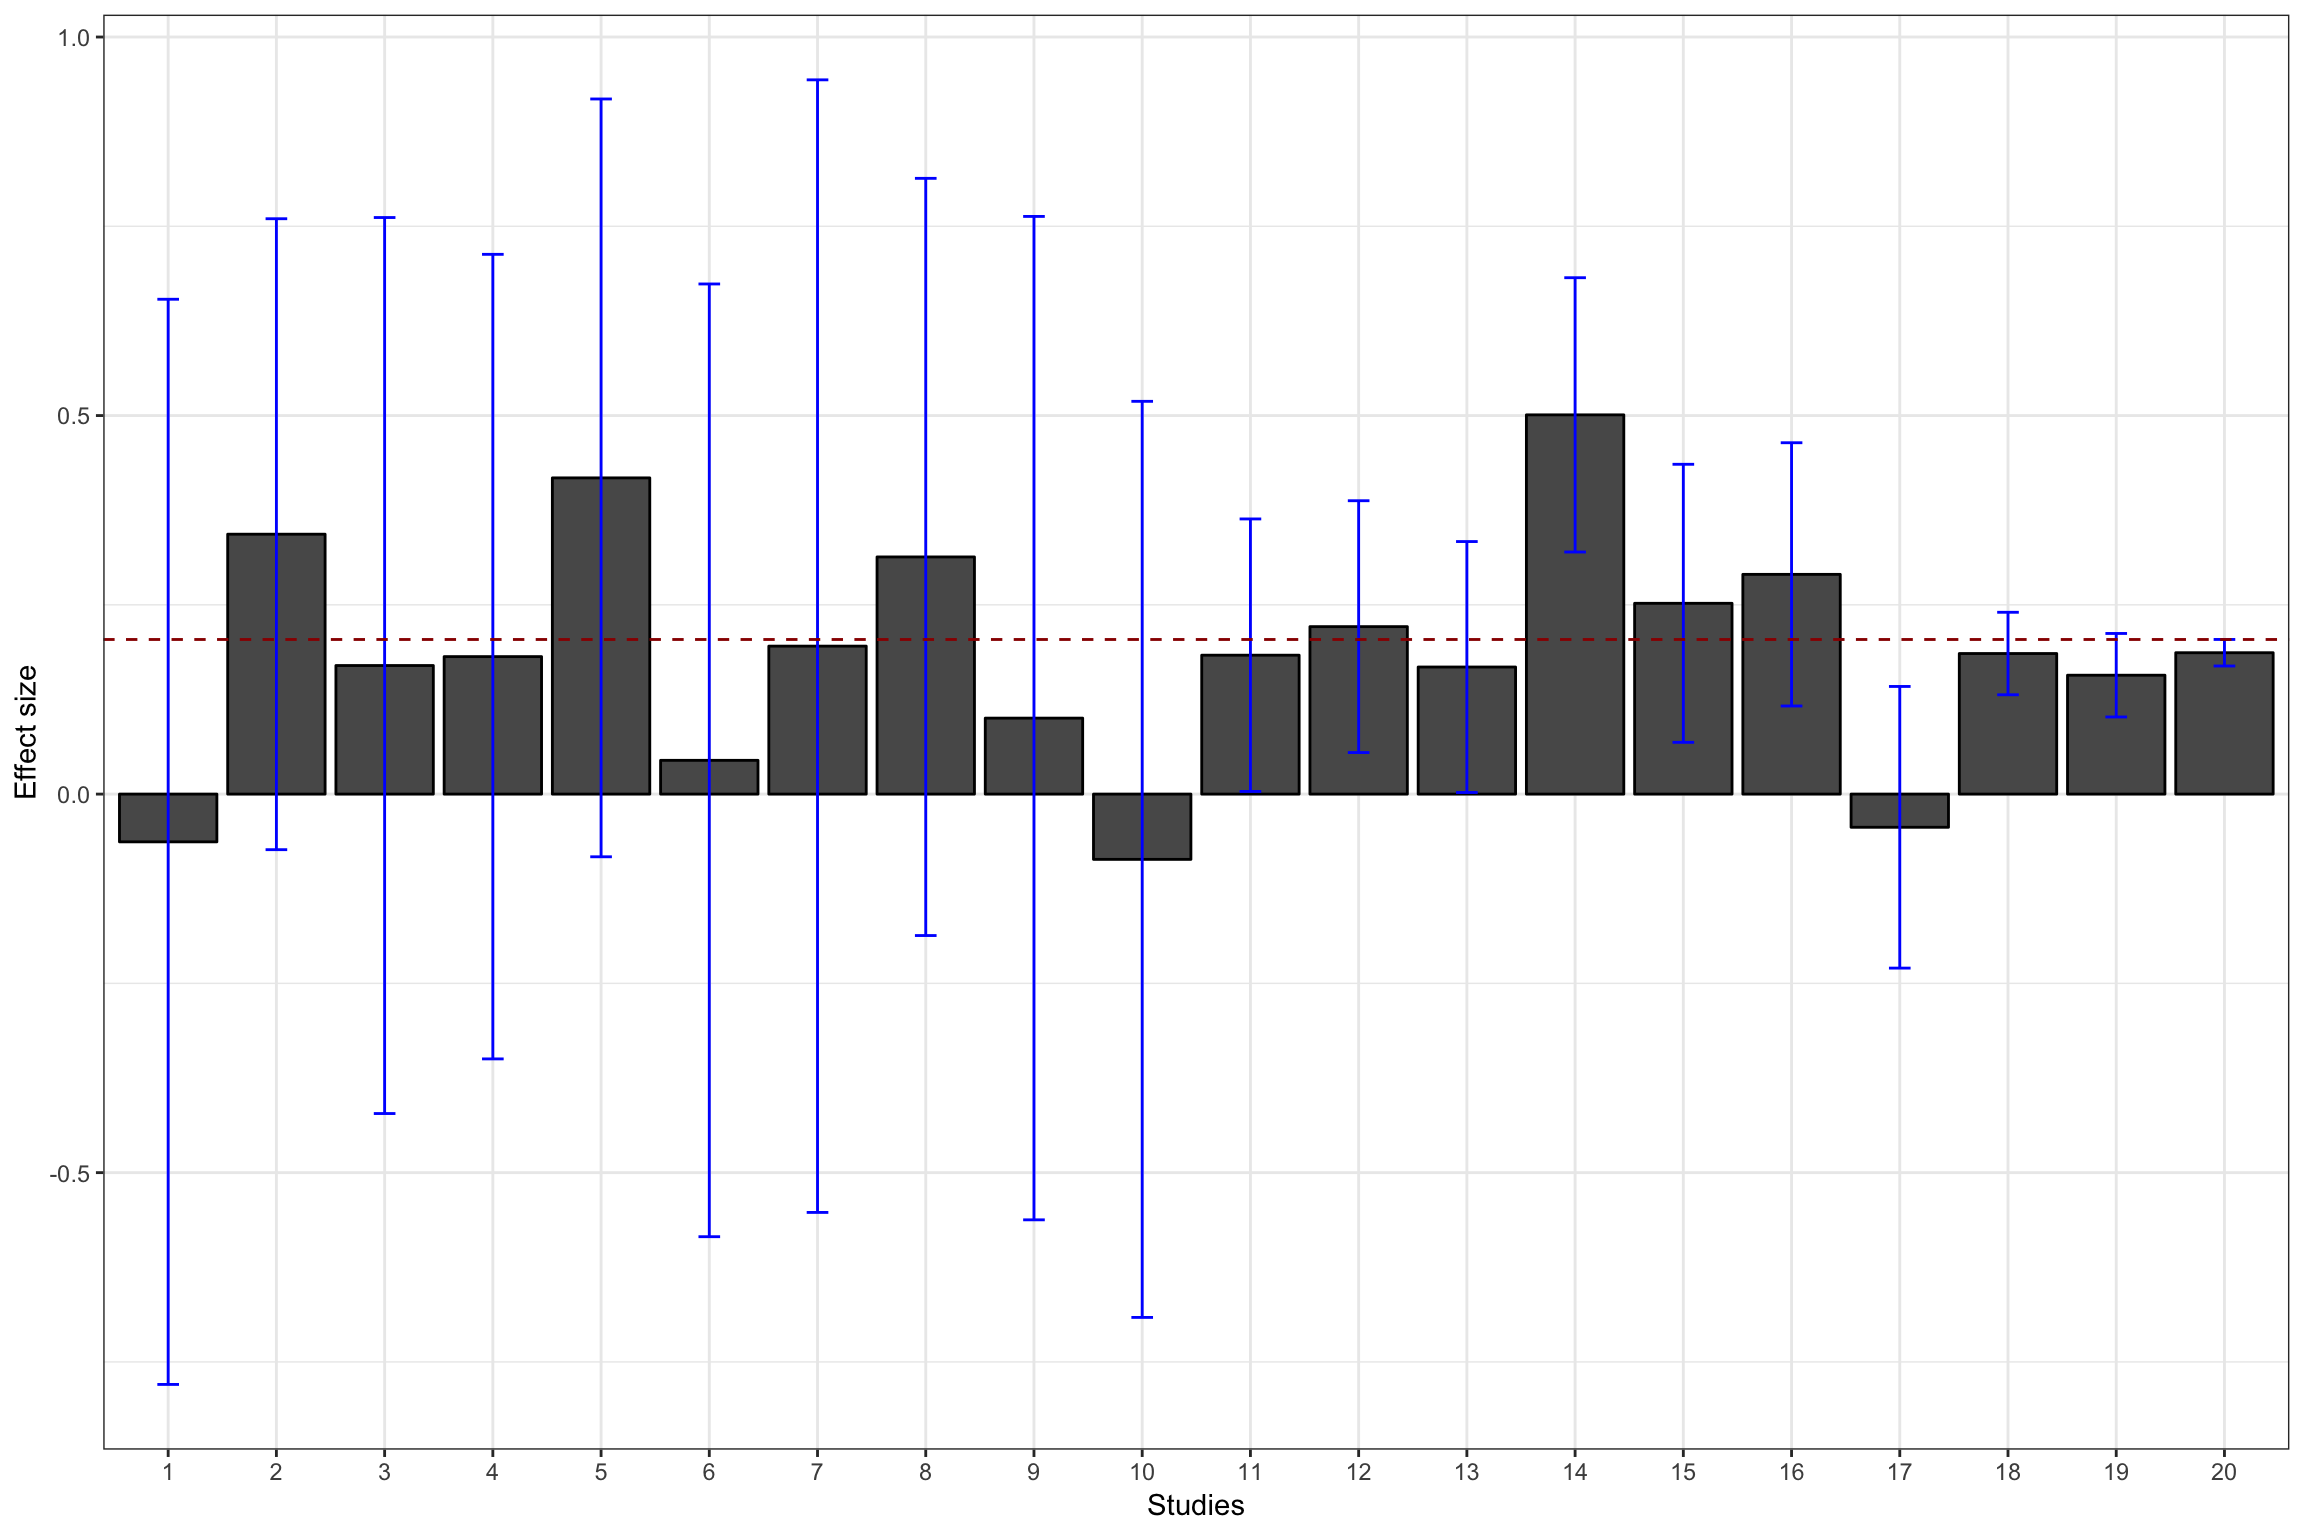
\includegraphics[width=0.33\linewidth]{STCI_files/figure-latex/metanoiseplot-1} }\subfloat[$\tau^2=$ 0.5\label{fig:metanoiseplot2}]{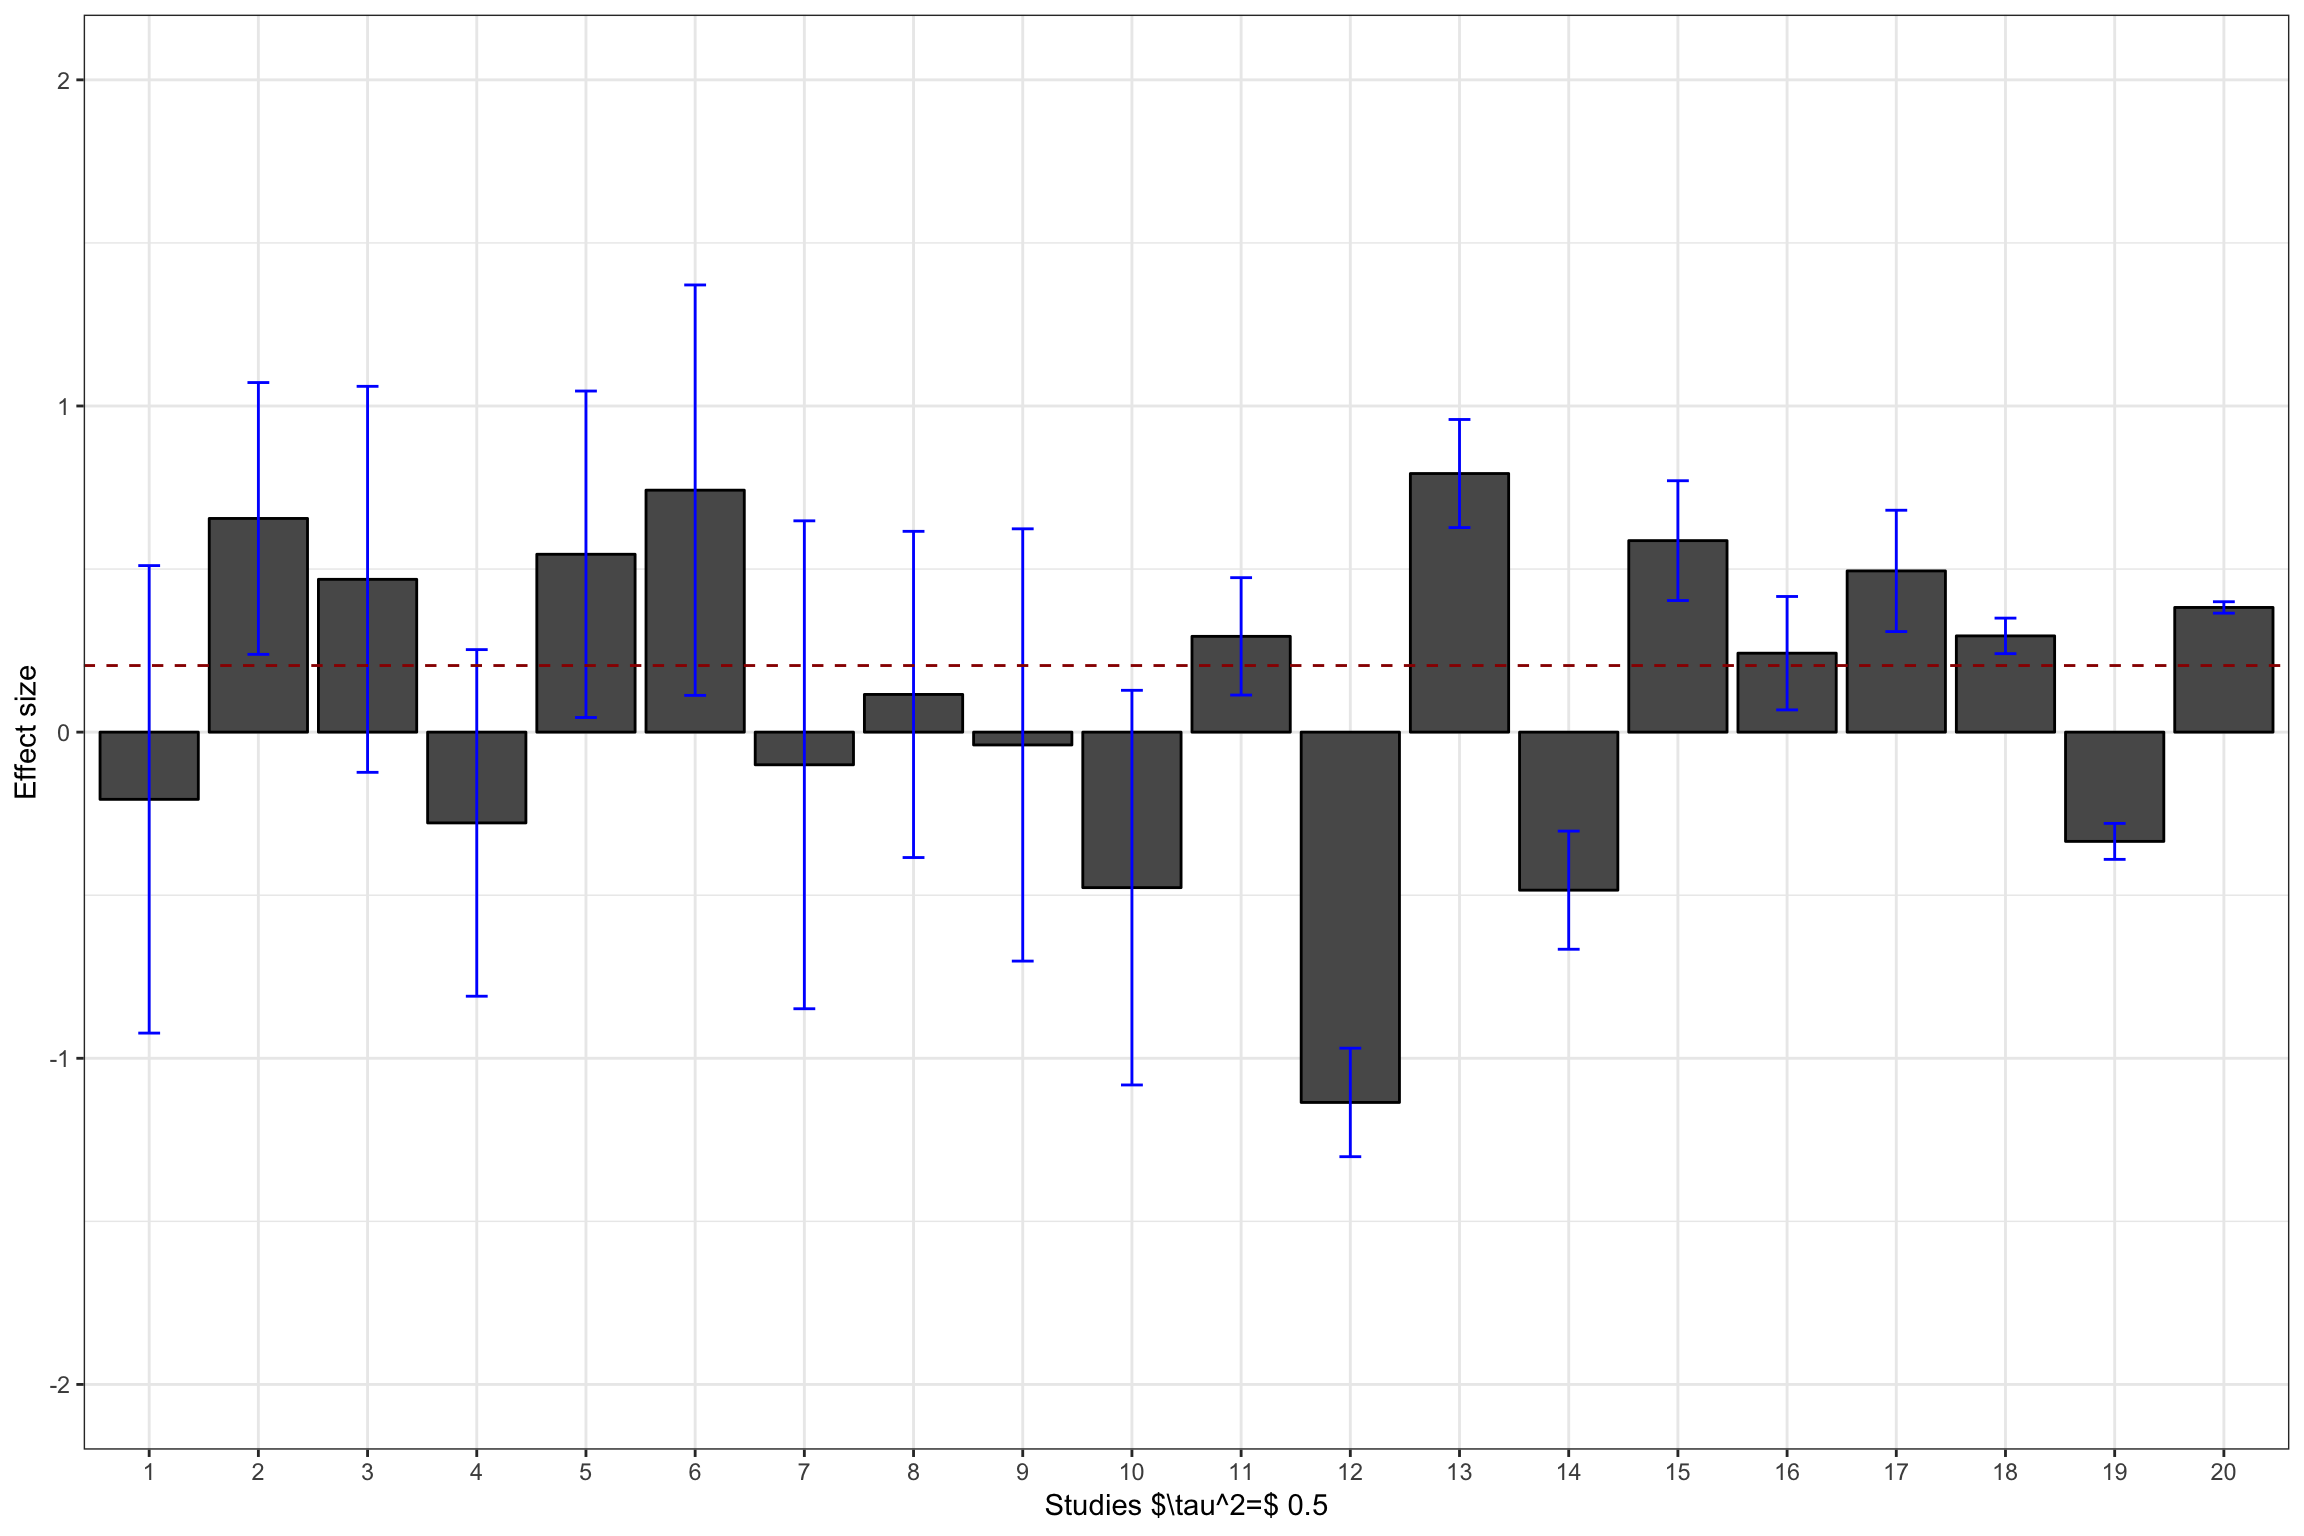
\includegraphics[width=0.33\linewidth]{STCI_files/figure-latex/metanoiseplot-2} }\subfloat[$\tau^2=$ 1\label{fig:metanoiseplot3}]{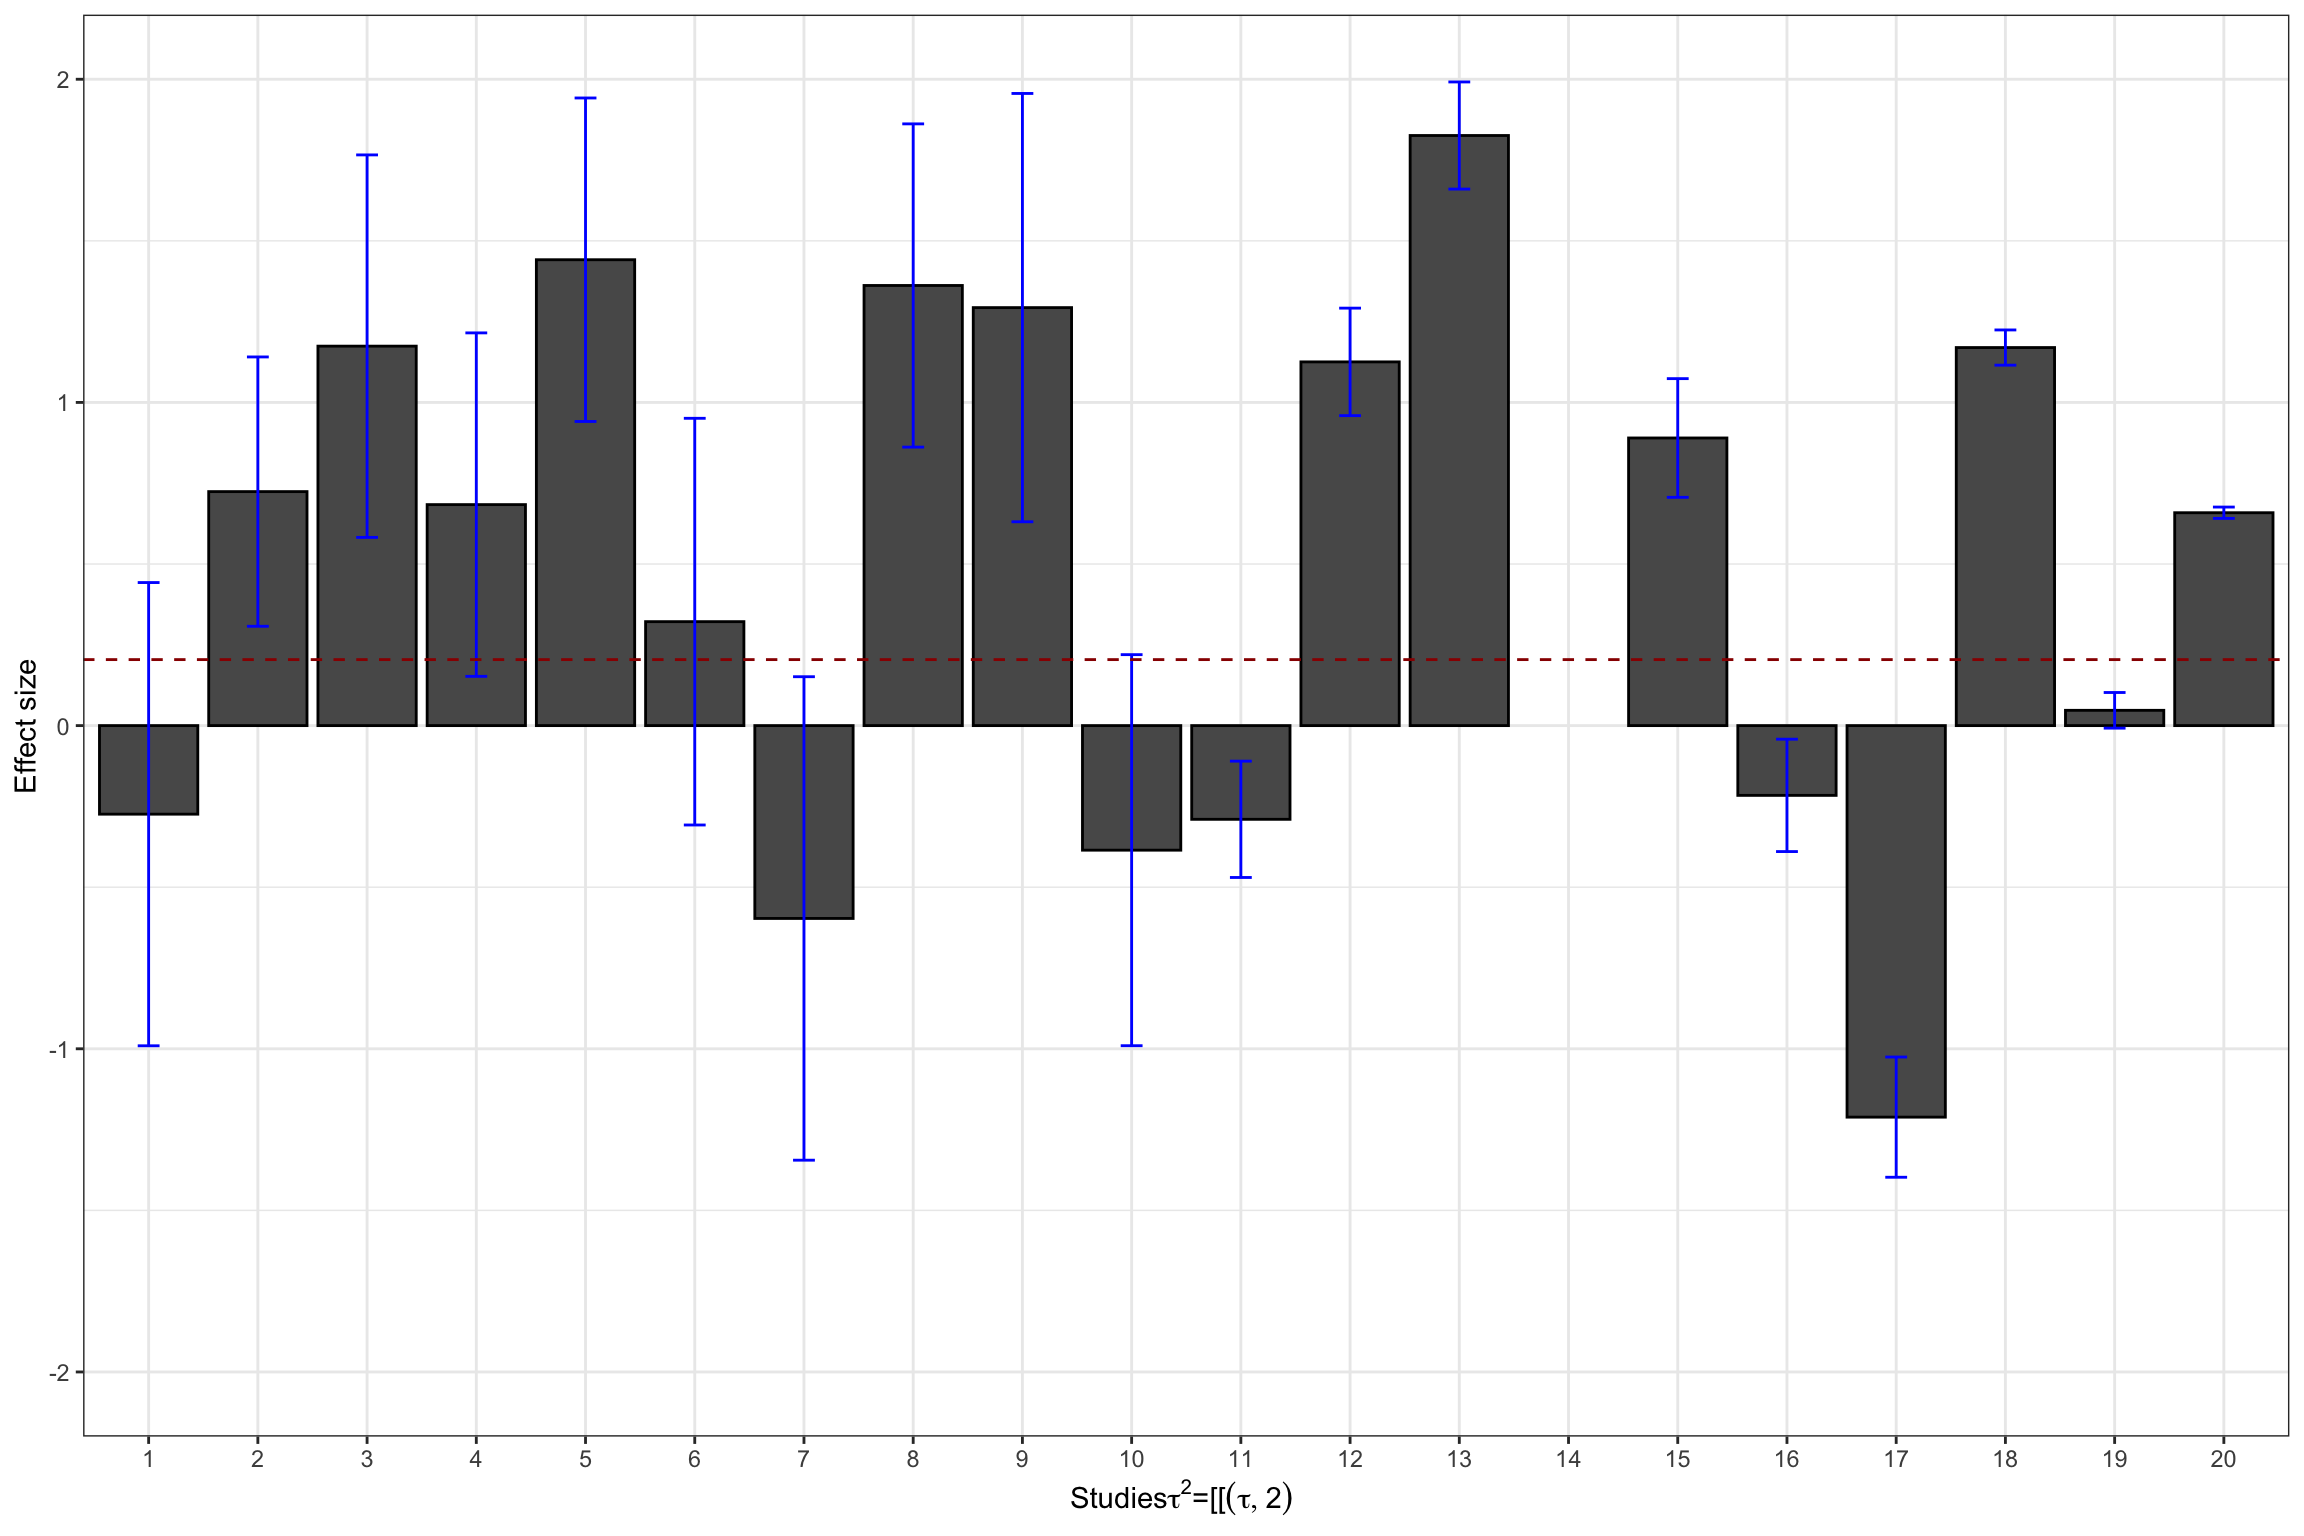
\includegraphics[width=0.33\linewidth]{STCI_files/figure-latex/metanoiseplot-3} }

}

\caption{Datasets with treatment effect heterogeneity}\label{fig:metanoiseplot}
\end{figure}

Let's see now how Hedge's estimator performs:

\begin{Shaded}
\begin{Highlighting}[]
\NormalTok{tau.}\FloatTok{2.}\NormalTok{theta.}\DecValTok{1}\NormalTok{ <-}\StringTok{ }\KeywordTok{tau.2}\NormalTok{(data.meta}\OperatorTok{$}\NormalTok{theta.}\DecValTok{1}\NormalTok{,data.meta}\OperatorTok{$}\NormalTok{se.ES}\OperatorTok{^}\DecValTok{2}\NormalTok{)}
\NormalTok{tau.}\FloatTok{2.}\NormalTok{theta.}\DecValTok{2}\NormalTok{ <-}\StringTok{ }\KeywordTok{tau.2}\NormalTok{(data.meta}\OperatorTok{$}\NormalTok{theta.}\DecValTok{2}\NormalTok{,data.meta}\OperatorTok{$}\NormalTok{se.ES}\OperatorTok{^}\DecValTok{2}\NormalTok{)}
\end{Highlighting}
\end{Shaded}

Hedges' estimates of \(\tau^2\) in our examples are thus 0.2 and 0.73
respectively, while the true values are, respectively 0.25 and 1.

\subsubsection{Estimating the average effect of the treatment taking
heterogeneity into
account}\label{estimating-the-average-effect-of-the-treatment-taking-heterogeneity-into-account}

Hedges proposes a new estimator for the average effect of the treatment,
an estimator that accounts for the additional noise due to heterogeneous
treatment effects accross sites.

\BeginKnitrBlock{definition}[Hedges Weighted Meta-Analytic Estimator]
\protect\hypertarget{def:Hmetaweights}{}{\label{def:Hmetaweights}
\iffalse (Hedges Weighted Meta-Analytic Estimator) \fi{} }Hedges
weighted meta-analytic estimator for in the presence of random effects
is \[
\bar{\theta}_H = \sum_{k=1}^Nv_k\hat{\theta}_k \text{ with } v_k=\frac{\frac{1}{\hat{\sigma}^2_k+\hat{\tau}^2}}{\sum_{k=1}^N\frac{1}{\hat{\sigma}^2_k+\hat{\tau}^2}}.
\]
\EndKnitrBlock{definition}

\begin{Shaded}
\begin{Highlighting}[]
\NormalTok{Hwmae <-}\StringTok{ }\ControlFlowTok{function}\NormalTok{(theta,sigma2,tau2)\{}
  \KeywordTok{return}\NormalTok{(}\KeywordTok{c}\NormalTok{(}\KeywordTok{weighted.mean}\NormalTok{(theta,(}\DecValTok{1}\OperatorTok{/}\NormalTok{sigma2)}\OperatorTok{/}\NormalTok{(}\KeywordTok{sum}\NormalTok{(}\DecValTok{1}\OperatorTok{/}\NormalTok{(sigma2}\OperatorTok{+}\NormalTok{tau2))),}\DecValTok{1}\OperatorTok{/}\KeywordTok{sum}\NormalTok{(}\DecValTok{1}\OperatorTok{/}\NormalTok{sigma2}\OperatorTok{+}\NormalTok{tau2))))}
\NormalTok{\}}
\NormalTok{ES.H.theta.}\DecValTok{1}\NormalTok{ <-}\StringTok{ }\KeywordTok{Hwmae}\NormalTok{(data.meta}\OperatorTok{$}\NormalTok{theta.}\DecValTok{1}\NormalTok{,data.meta}\OperatorTok{$}\NormalTok{se.ES}\OperatorTok{^}\DecValTok{2}\NormalTok{,tau.}\FloatTok{2.}\NormalTok{theta.}\DecValTok{1}\NormalTok{)}
\NormalTok{ES.H.theta.}\DecValTok{2}\NormalTok{ <-}\StringTok{ }\KeywordTok{Hwmae}\NormalTok{(data.meta}\OperatorTok{$}\NormalTok{theta.}\DecValTok{2}\NormalTok{,data.meta}\OperatorTok{$}\NormalTok{se.ES}\OperatorTok{^}\DecValTok{2}\NormalTok{,tau.}\FloatTok{2.}\NormalTok{theta.}\DecValTok{2}\NormalTok{)}
\end{Highlighting}
\end{Shaded}

\BeginKnitrBlock{example}
\protect\hypertarget{exm:unnamed-chunk-136}{}{\label{exm:unnamed-chunk-136}
}Let's see how Hedges estimator performs in our example.
\EndKnitrBlock{example} Hedges' estimates of the average effect size is
equal to 0.3 and 0.65 respectively, while the true value is 0.2. The
main problem with Hedges' estimator when treatment effects are
heterogeneous is that very large effects for the more precise estimators
dramatically affect the estimate.

\BeginKnitrBlock{remark}
\iffalse{} {Remark. } \fi{}Hedges' estimate of \(\tau^2\) is slightly
negative, which is problem, since a variance is always positive. Other
estimators of \(\tau^2\) have been proposed in the literature to account
for this fact and to respond to various shortcomings of Hedges'
approach. We will present them succinctly since they are part of the
\texttt{metafor} package. These other estimators have bames such as .
They are very well described in this
\href{http://www.edii.uclm.es/~useR-2013/Tutorials/kovalchik/kovalchik_meta_tutorial.pdf}{amazing
set of slides}. Besides Hedges' (denoted `HE' in R), the other
estimators are named:
\EndKnitrBlock{remark}

\begin{itemize}
\tightlist
\item
  DerSimonian-Laird (`DL')
\item
  Hunter-Schmidt (`HS')
\item
  Sidik-Jonkman (`SJ')
\item
  Maximum-likelihood (`ML')
\item
  Restricted maximum-likelihood (`REML')
\item
  Empirical Bayes (`EB')
\end{itemize}

I'll detail how they work later.

\textbf{\textsc{Detail other estimators of tau.}}

\BeginKnitrBlock{example}
\protect\hypertarget{exm:unnamed-chunk-138}{}{\label{exm:unnamed-chunk-138}
}For the moment, let's see how they perform in our numerical example.
\EndKnitrBlock{example}

\begin{Shaded}
\begin{Highlighting}[]
\NormalTok{estimators <-}\StringTok{ }\KeywordTok{c}\NormalTok{(}\StringTok{"DL"}\NormalTok{, }\StringTok{"REML"}\NormalTok{, }\StringTok{"HE"}\NormalTok{, }\StringTok{"HS"}\NormalTok{, }\StringTok{"SJ"}\NormalTok{, }\StringTok{"ML"}\NormalTok{, }\StringTok{"EB"}\NormalTok{)}
\NormalTok{meta.example.RE.theta.}\FloatTok{1.}\NormalTok{tau2 <-}\StringTok{ }\KeywordTok{sapply}\NormalTok{(estimators,}\ControlFlowTok{function}\NormalTok{(method)\{}\KeywordTok{return}\NormalTok{(}\KeywordTok{rma}\NormalTok{(}\DataTypeTok{yi =}\NormalTok{ data.meta}\OperatorTok{$}\NormalTok{theta.}\DecValTok{1}\NormalTok{,}\DataTypeTok{vi=}\NormalTok{data.meta}\OperatorTok{$}\NormalTok{var.ES,}\DataTypeTok{method=}\NormalTok{method)}\OperatorTok{$}\NormalTok{tau2)\})}
\NormalTok{meta.example.RE.theta.}\FloatTok{2.}\NormalTok{tau2 <-}\StringTok{ }\KeywordTok{sapply}\NormalTok{(estimators,}\ControlFlowTok{function}\NormalTok{(method)\{}\KeywordTok{return}\NormalTok{(}\KeywordTok{rma}\NormalTok{(}\DataTypeTok{yi =}\NormalTok{ data.meta}\OperatorTok{$}\NormalTok{theta.}\DecValTok{2}\NormalTok{,}\DataTypeTok{vi=}\NormalTok{data.meta}\OperatorTok{$}\NormalTok{var.ES,}\DataTypeTok{method=}\NormalTok{method)}\OperatorTok{$}\NormalTok{tau2)\})}
\CommentTok{#meta.example.RE <- sapply(estimators,function(method)\{return(rma(yi = data.meta$theta.1,vi=data.meta$var.ES,method=method))\})}
\CommentTok{#meta.example.RE.tau2.test <- unlist(lapply(meta.example.RE,'[[','tau2'))}

\NormalTok{result.RE <-}\StringTok{ }\KeywordTok{data.frame}\NormalTok{(}\DataTypeTok{Method=}\KeywordTok{rep}\NormalTok{(estimators,}\DecValTok{2}\NormalTok{),}\DataTypeTok{tau2hat=}\KeywordTok{c}\NormalTok{(meta.example.RE.theta.}\FloatTok{1.}\NormalTok{tau2,meta.example.RE.theta.}\FloatTok{2.}\NormalTok{tau2),}\DataTypeTok{tau2=}\KeywordTok{c}\NormalTok{(}\KeywordTok{rep}\NormalTok{(tau[[}\DecValTok{1}\NormalTok{]]}\OperatorTok{^}\DecValTok{2}\NormalTok{,}\KeywordTok{length}\NormalTok{(estimators)),}\KeywordTok{rep}\NormalTok{(tau[[}\DecValTok{2}\NormalTok{]]}\OperatorTok{^}\DecValTok{2}\NormalTok{,}\KeywordTok{length}\NormalTok{(estimators))))}

\KeywordTok{ggplot}\NormalTok{(}\DataTypeTok{data=}\NormalTok{result.RE, }\KeywordTok{aes}\NormalTok{(}\DataTypeTok{x=}\NormalTok{Method, }\DataTypeTok{y=}\NormalTok{tau2hat, }\DataTypeTok{fill=}\KeywordTok{as.factor}\NormalTok{(tau2))) }\OperatorTok{+}
\StringTok{    }\KeywordTok{geom_bar}\NormalTok{(}\DataTypeTok{stat=}\StringTok{"identity"}\NormalTok{, }\DataTypeTok{position=}\KeywordTok{position_dodge}\NormalTok{())}\OperatorTok{+}
\StringTok{    }\KeywordTok{ylim}\NormalTok{(}\DecValTok{0}\NormalTok{,}\DecValTok{1}\NormalTok{)}
\end{Highlighting}
\end{Shaded}

\begin{figure}[htbp]

{\centering 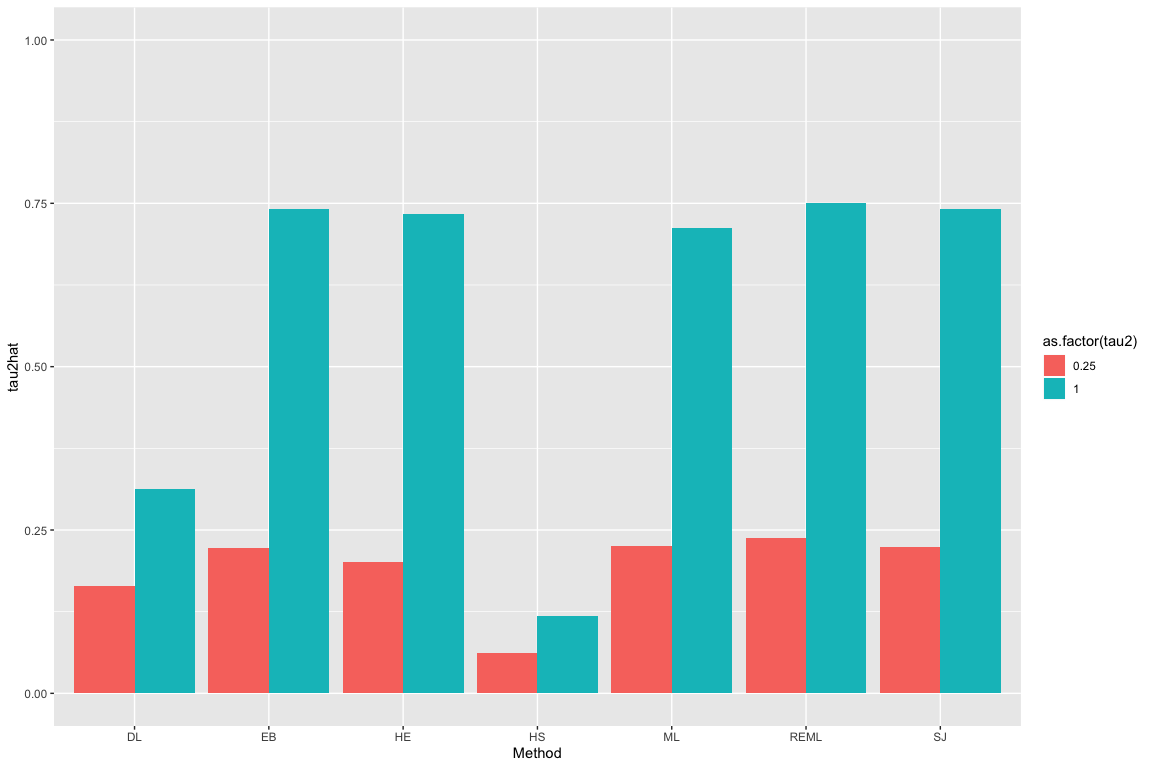
\includegraphics[width=0.6\linewidth]{STCI_files/figure-latex/RandomOthersTau-1} 

}

\caption{Various estimators of $\tau^2$}\label{fig:RandomOthersTau}
\end{figure}

We are ready to estimate the overall treatment effect using random
effects.

\begin{Shaded}
\begin{Highlighting}[]
\NormalTok{estimators <-}\StringTok{ }\KeywordTok{c}\NormalTok{(}\StringTok{"DL"}\NormalTok{, }\StringTok{"REML"}\NormalTok{, }\StringTok{"HE"}\NormalTok{, }\StringTok{"HS"}\NormalTok{, }\StringTok{"SJ"}\NormalTok{, }\StringTok{"ML"}\NormalTok{, }\StringTok{"EB"}\NormalTok{)}
\NormalTok{meta.example.RE.theta.}\FloatTok{1.}\NormalTok{ES <-}\StringTok{ }\KeywordTok{sapply}\NormalTok{(estimators,}\ControlFlowTok{function}\NormalTok{(method)\{}\KeywordTok{return}\NormalTok{(}\KeywordTok{rma}\NormalTok{(}\DataTypeTok{yi =}\NormalTok{ data.meta}\OperatorTok{$}\NormalTok{theta.}\DecValTok{1}\NormalTok{,}\DataTypeTok{vi=}\NormalTok{data.meta}\OperatorTok{$}\NormalTok{var.ES,}\DataTypeTok{method=}\NormalTok{method)}\OperatorTok{$}\NormalTok{beta)\})}
\NormalTok{meta.example.RE.theta.}\FloatTok{2.}\NormalTok{ES <-}\StringTok{ }\KeywordTok{sapply}\NormalTok{(estimators,}\ControlFlowTok{function}\NormalTok{(method)\{}\KeywordTok{return}\NormalTok{(}\KeywordTok{rma}\NormalTok{(}\DataTypeTok{yi =}\NormalTok{ data.meta}\OperatorTok{$}\NormalTok{theta.}\DecValTok{2}\NormalTok{,}\DataTypeTok{vi=}\NormalTok{data.meta}\OperatorTok{$}\NormalTok{var.ES,}\DataTypeTok{method=}\NormalTok{method)}\OperatorTok{$}\NormalTok{beta)\})}
\CommentTok{#meta.example.RE.tau2.test <- unlist(lapply(meta.example.RE,'[[','tau2'))}

\NormalTok{result.RE}\OperatorTok{$}\NormalTok{ES.RE <-}\StringTok{ }\KeywordTok{c}\NormalTok{(meta.example.RE.theta.}\FloatTok{1.}\NormalTok{ES,meta.example.RE.theta.}\FloatTok{2.}\NormalTok{ES)}

\KeywordTok{ggplot}\NormalTok{(}\DataTypeTok{data=}\NormalTok{result.RE, }\KeywordTok{aes}\NormalTok{(}\DataTypeTok{x=}\NormalTok{Method, }\DataTypeTok{y=}\NormalTok{ES.RE, }\DataTypeTok{fill=}\KeywordTok{as.factor}\NormalTok{(tau2))) }\OperatorTok{+}
\StringTok{    }\KeywordTok{geom_bar}\NormalTok{(}\DataTypeTok{stat=}\StringTok{"identity"}\NormalTok{, }\DataTypeTok{position=}\KeywordTok{position_dodge}\NormalTok{())}
\end{Highlighting}
\end{Shaded}

\begin{figure}[htbp]

{\centering 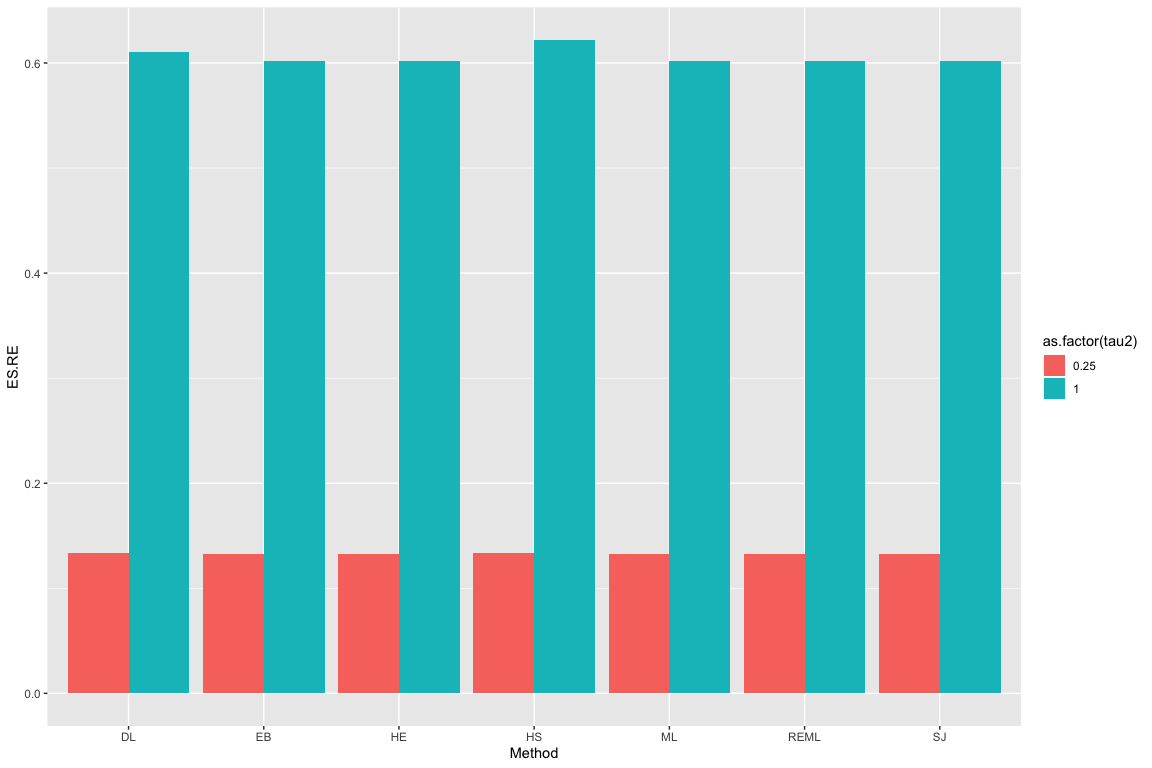
\includegraphics[width=0.6\linewidth]{STCI_files/figure-latex/RandomOthersES-1} 

}

\caption{Various estimators of the treatment effect with random effects}\label{fig:RandomOthersES}
\end{figure}

\subsubsection{Other estimators of inter-site
variability}\label{other-estimators-of-inter-site-variability}

\(\tau^2\) is a pretty difficult measure of treatment effect
heterogeneity to interpret. That's why other indicators have been built
that are easier to interpret. We are going to review several of them in
this section.

The first alternative or complement to \(\tau^2\) is Higgin's \(I^2\):

\begin{align*}
  I^2 & = \frac{Q-(N-1)}{Q}*100
\end{align*}

The interpretation of \(I^2\) is pretty straightforward: it is the
distance between the actual value of the \(Q\) statistic and its value
under the null of treatment effect homogeneity (it is equal to the
number of studies \(N\), with a correction for degress of freedom). It
can also be interpreted as the fraction of the overall variance
(remember that \(Q\) is the sum of variance ratios) that is not
explained by within study sampling noise.

Another complement to \(\tau^2\) is \(H^2\):

\begin{align*}
  H^2 & = \frac{Q}{N-1}
\end{align*}

If \(H^2\) is above one, then there is unexplained heterogeneity, again
by the fact that \(Q\) has mean \(N-1\) under the null of treatment
effect homogeneity.

Finally, we can also define the Intra Class Correlation (\(ICC\)), which
precisely measures the share of total variance attributable to treatment
effect heterogeneity:

\begin{align*}
  ICC & = \frac{\tau^2}{\tau^2+S^2}
\end{align*}

Where \(S^2\) is the amount of variance due to sampling noise. An
estimator for \(S^2\) is:

\begin{align*}
  S^2 & = \frac{(N-1)\sum_{k=1}^N\frac{1}{\sigma^2_k}}{(\sum_{k=1}^N\frac{1}{\sigma^2_k})^2-\sum_{k=1}^N(\frac{1}{\sigma^2_k})^2}.
\end{align*}

\textbf{\textsc{I do not understand the formula for \(S^2\). Why does it
estimate what we want? I'd take the average variance.}}

\(ICC\) and \(I^2\) are related by the following very simple relation:
\(I^2=ICC*100\).

\BeginKnitrBlock{example}
\protect\hypertarget{exm:unnamed-chunk-139}{}{\label{exm:unnamed-chunk-139}
}Let's see how these three estimators look like in our example. The cool
thing is that \texttt{rma} computes these estimators by default, so that
a simple call to \texttt{summary()} is going to show them. The default
random effects estimator is \texttt{REML}, which is deemed to be the
best of them all according to simulations
\href{https://journals.sagepub.com/doi/abs/10.3102/10769986030003261}{(Viechtbauer,
2002)}.
\EndKnitrBlock{example}

\begin{Shaded}
\begin{Highlighting}[]
\NormalTok{meta.example.RE.ES <-}\StringTok{ }\KeywordTok{rma}\NormalTok{(}\DataTypeTok{yi =}\NormalTok{ data.meta}\OperatorTok{$}\NormalTok{ES,}\DataTypeTok{vi=}\NormalTok{data.meta}\OperatorTok{$}\NormalTok{var.ES)}
\NormalTok{meta.example.RE.theta.}\DecValTok{1}\NormalTok{ <-}\StringTok{ }\KeywordTok{rma}\NormalTok{(}\DataTypeTok{yi =}\NormalTok{ data.meta}\OperatorTok{$}\NormalTok{theta.}\DecValTok{1}\NormalTok{,}\DataTypeTok{vi=}\NormalTok{data.meta}\OperatorTok{$}\NormalTok{var.ES)}
\NormalTok{meta.example.RE.theta.}\DecValTok{2}\NormalTok{ <-}\StringTok{ }\KeywordTok{rma}\NormalTok{(}\DataTypeTok{yi =}\NormalTok{ data.meta}\OperatorTok{$}\NormalTok{theta.}\DecValTok{2}\NormalTok{,}\DataTypeTok{vi=}\NormalTok{data.meta}\OperatorTok{$}\NormalTok{var.ES)}

\NormalTok{tau2.hat <-}\StringTok{ }\KeywordTok{c}\NormalTok{(meta.example.RE.ES}\OperatorTok{$}\NormalTok{tau2,meta.example.RE.theta.}\DecValTok{1}\OperatorTok{$}\NormalTok{tau2,meta.example.RE.theta.}\DecValTok{2}\OperatorTok{$}\NormalTok{tau2)}
\NormalTok{I2 <-}\StringTok{  }\KeywordTok{c}\NormalTok{(meta.example.RE.theta.}\DecValTok{1}\OperatorTok{$}\NormalTok{I2,meta.example.RE.theta.}\DecValTok{2}\OperatorTok{$}\NormalTok{I2,meta.example.RE.ES}\OperatorTok{$}\NormalTok{I2)}
\NormalTok{H2 <-}\StringTok{  }\KeywordTok{c}\NormalTok{(meta.example.RE.theta.}\DecValTok{1}\OperatorTok{$}\NormalTok{H2,meta.example.RE.theta.}\DecValTok{2}\OperatorTok{$}\NormalTok{H2,meta.example.RE.ES}\OperatorTok{$}\NormalTok{H2)}

\CommentTok{# illustration of results returned by summary}
\KeywordTok{summary}\NormalTok{(meta.example.RE.theta.}\DecValTok{2}\NormalTok{)}
\end{Highlighting}
\end{Shaded}

\begin{verbatim}
## 
## Random-Effects Model (k = 20; tau^2 estimator: REML)
## 
##   logLik  deviance       AIC       BIC      AICc  
## -24.7208   49.4417   53.4417   55.3305   54.1917  
## 
## tau^2 (estimated amount of total heterogeneity): 0.7507 (SE = 0.2583)
## tau (square root of estimated tau^2 value):      0.8664
## I^2 (total heterogeneity / total variability):   99.59%
## H^2 (total variability / sampling variability):  241.82
## 
## Test for Heterogeneity: 
## Q(df = 19) = 1927.7020, p-val < .0001
## 
## Model Results:
## 
## estimate      se    zval    pval   ci.lb   ci.ub    
##   0.6015  0.1997  3.0127  0.0026  0.2102  0.9929  **
## 
## ---
## Signif. codes:  0 '***' 0.001 '**' 0.01 '*' 0.05 '.' 0.1 ' ' 1
\end{verbatim}

The estimate of \(I^2\) in our example is of 0 when \(\tau^2\) is equal
to 0, of 98.71 when \(\tau^2\) is equal to 0.25 and of 99.59 when
\(\tau^2\) is equal to 1. The estimate of \(H^2\) in our example is of 1
when \(\tau^2\) is equal to 0, of 77.4 when \(\tau^2\) is equal to 0.25
and of 241.82 when \(\tau^2\) is equal to 1.

\subsubsection{Presenting the results of a random effects
meta-analysis}\label{presenting-the-results-of-a-random-effects-meta-analysis}

In order to illustrate the results of a random effects meta-analysis,
you can first show the forest plot. Let's see how it works in our
example:

\begin{Shaded}
\begin{Highlighting}[]
\KeywordTok{forest}\NormalTok{(meta.example.RE.ES,}\DataTypeTok{slab =} \KeywordTok{paste}\NormalTok{(}\StringTok{'Study'}\NormalTok{,data.meta}\OperatorTok{$}\NormalTok{id,}\DataTypeTok{sep=}\StringTok{' '}\NormalTok{),}\DataTypeTok{xlab=}\KeywordTok{expression}\NormalTok{(}\KeywordTok{paste}\NormalTok{(}\StringTok{'Estimated Meta-analytic Parameter,'}\NormalTok{,tau}\OperatorTok{^}\DecValTok{2}\NormalTok{,}\DecValTok{0}\NormalTok{,}\DataTypeTok{sep=}\StringTok{' '}\NormalTok{)))}
\KeywordTok{forest}\NormalTok{(meta.example.RE.theta.}\DecValTok{1}\NormalTok{,}\DataTypeTok{slab =} \KeywordTok{paste}\NormalTok{(}\StringTok{'Study'}\NormalTok{,data.meta}\OperatorTok{$}\NormalTok{id,}\DataTypeTok{sep=}\StringTok{' '}\NormalTok{),}\DataTypeTok{xlab=}\KeywordTok{expression}\NormalTok{(}\KeywordTok{paste}\NormalTok{(}\StringTok{'Estimated Meta-analytic Parameter,'}\NormalTok{,tau}\OperatorTok{^}\DecValTok{2}\NormalTok{,}\StringTok{'='}\NormalTok{,}\StringTok{'0.25'}\NormalTok{,}\DataTypeTok{sep=}\StringTok{' '}\NormalTok{)))}
\KeywordTok{forest}\NormalTok{(meta.example.RE.theta.}\DecValTok{2}\NormalTok{,}\DataTypeTok{slab =} \KeywordTok{paste}\NormalTok{(}\StringTok{'Study'}\NormalTok{,data.meta}\OperatorTok{$}\NormalTok{id,}\DataTypeTok{sep=}\StringTok{' '}\NormalTok{),}\DataTypeTok{xlab=}\KeywordTok{expression}\NormalTok{(}\KeywordTok{paste}\NormalTok{(}\StringTok{'Estimated Meta-analytic Parameter,'}\NormalTok{,tau}\OperatorTok{^}\DecValTok{2}\NormalTok{,}\StringTok{'='}\NormalTok{,}\StringTok{'1'}\NormalTok{,}\DataTypeTok{sep=}\StringTok{' '}\NormalTok{)))}
\end{Highlighting}
\end{Shaded}

\begin{figure}[htbp]

{\centering \subfloat[$\tau^2=$0\label{fig:RERMAmetafor1}]{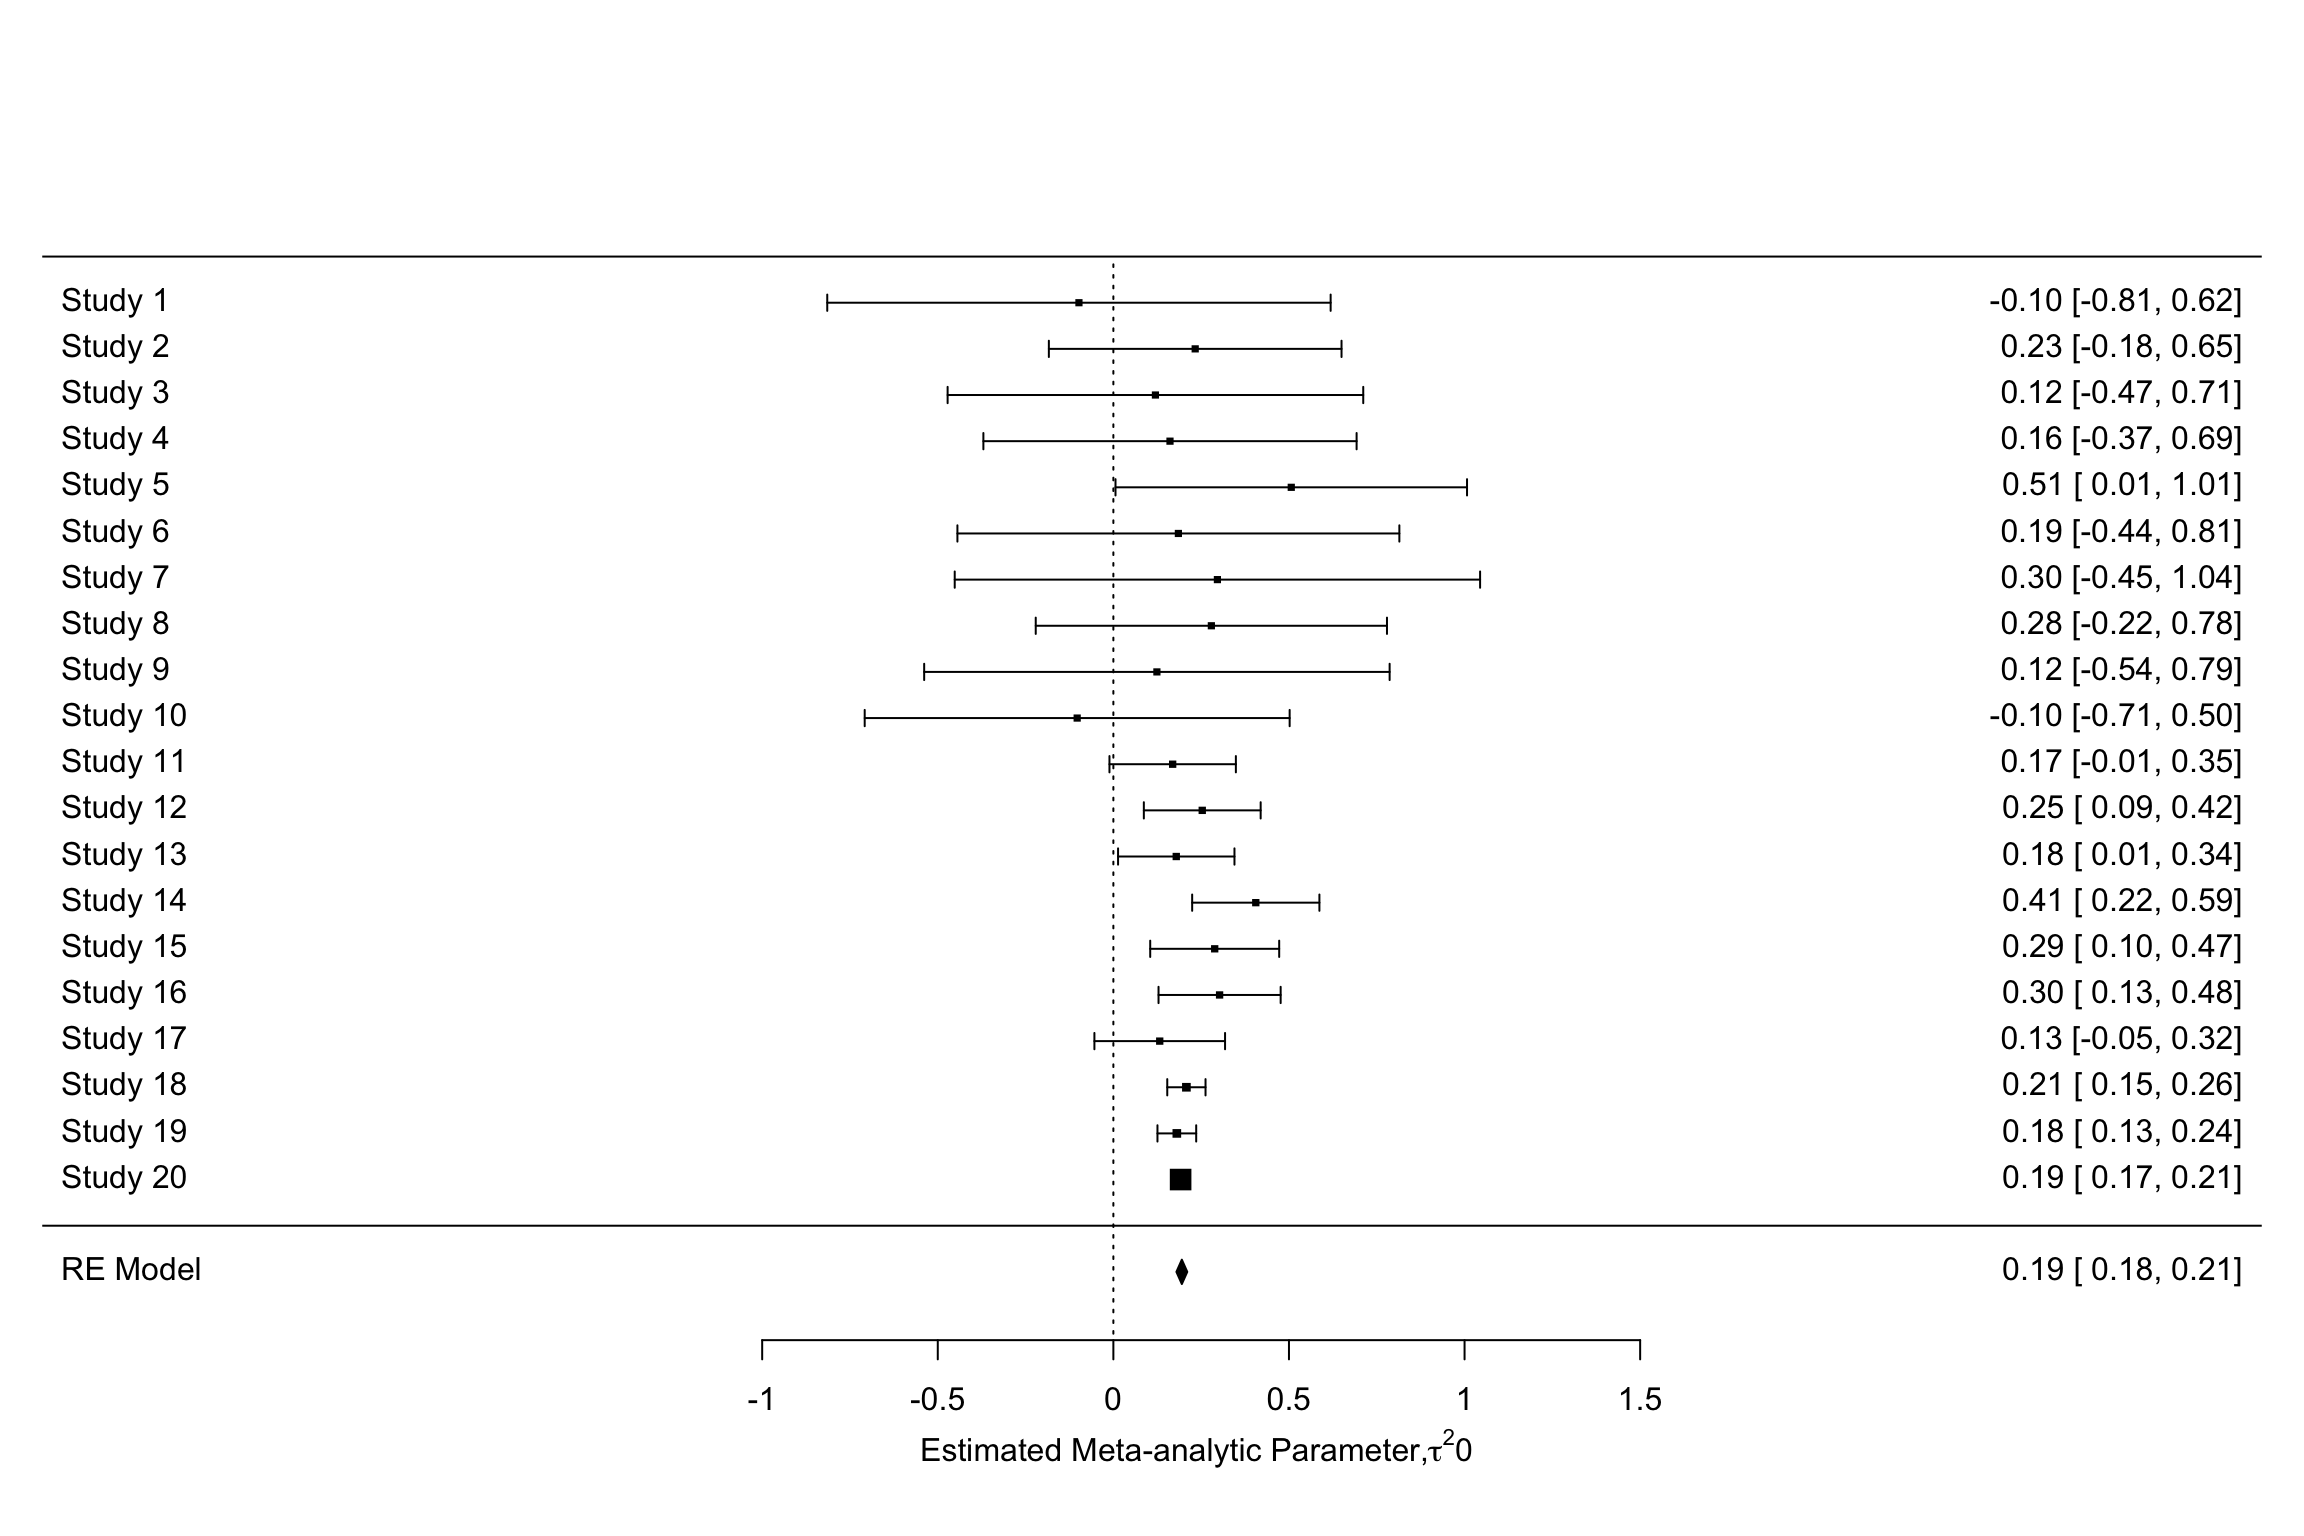
\includegraphics[width=0.33\linewidth]{STCI_files/figure-latex/RERMAmetafor-1} }\subfloat[$\tau^2=$0.25\label{fig:RERMAmetafor2}]{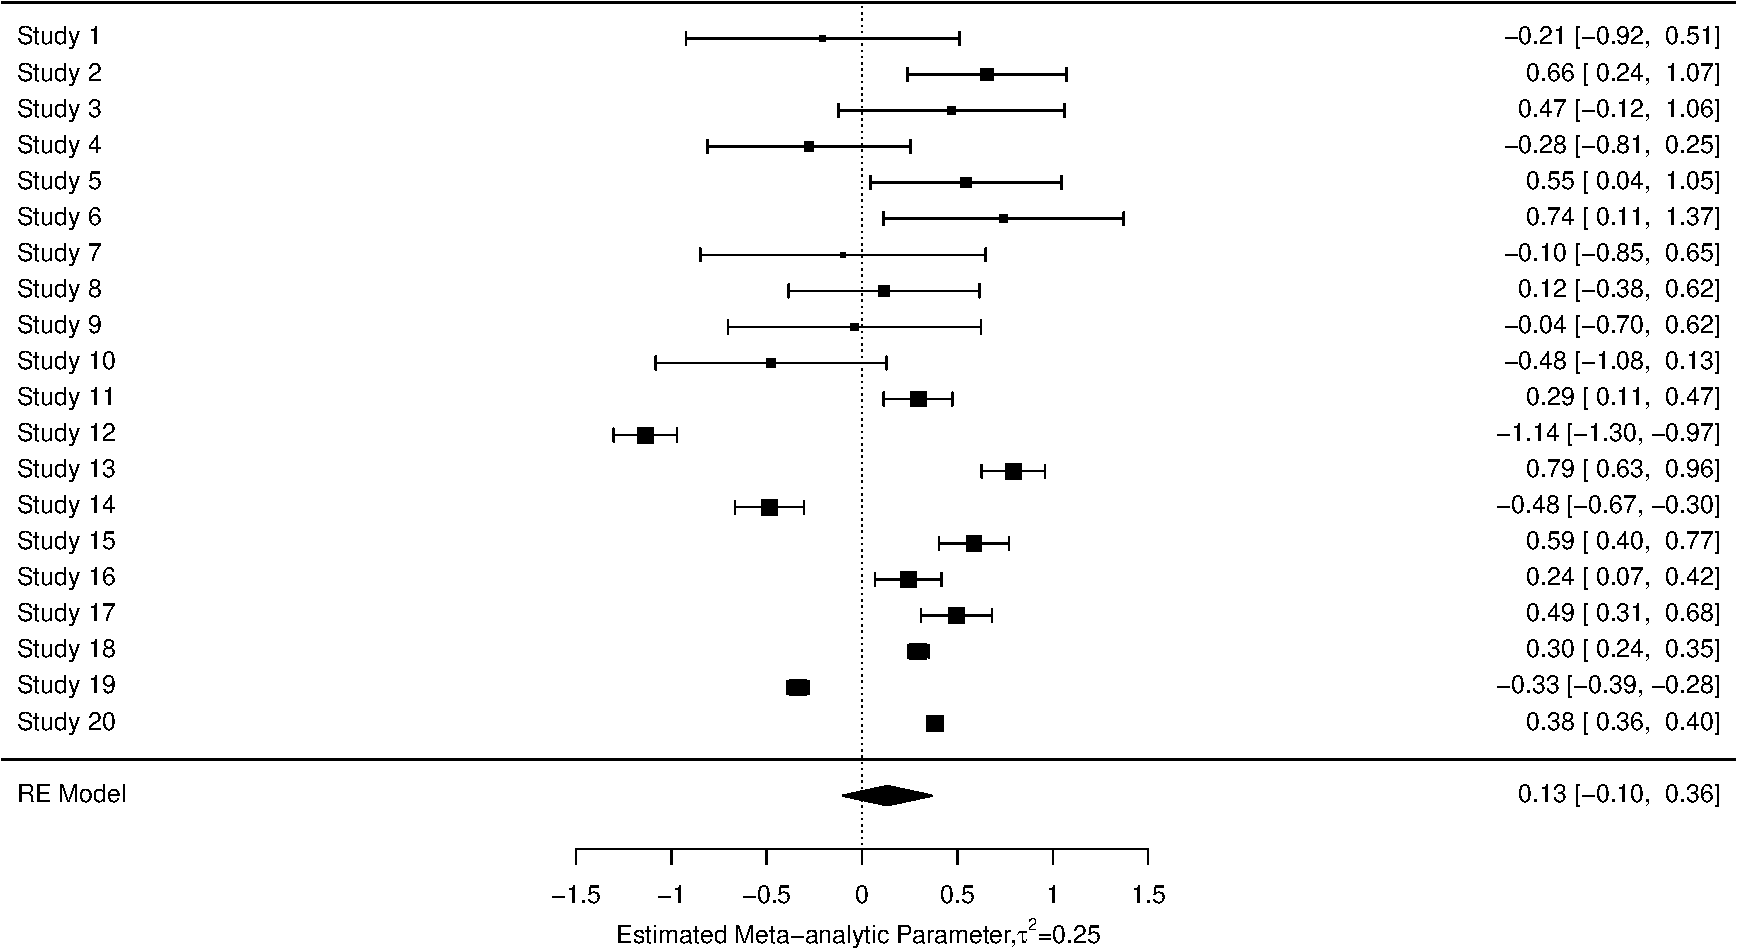
\includegraphics[width=0.33\linewidth]{STCI_files/figure-latex/RERMAmetafor-2} }\subfloat[$\tau^2=$1\label{fig:RERMAmetafor3}]{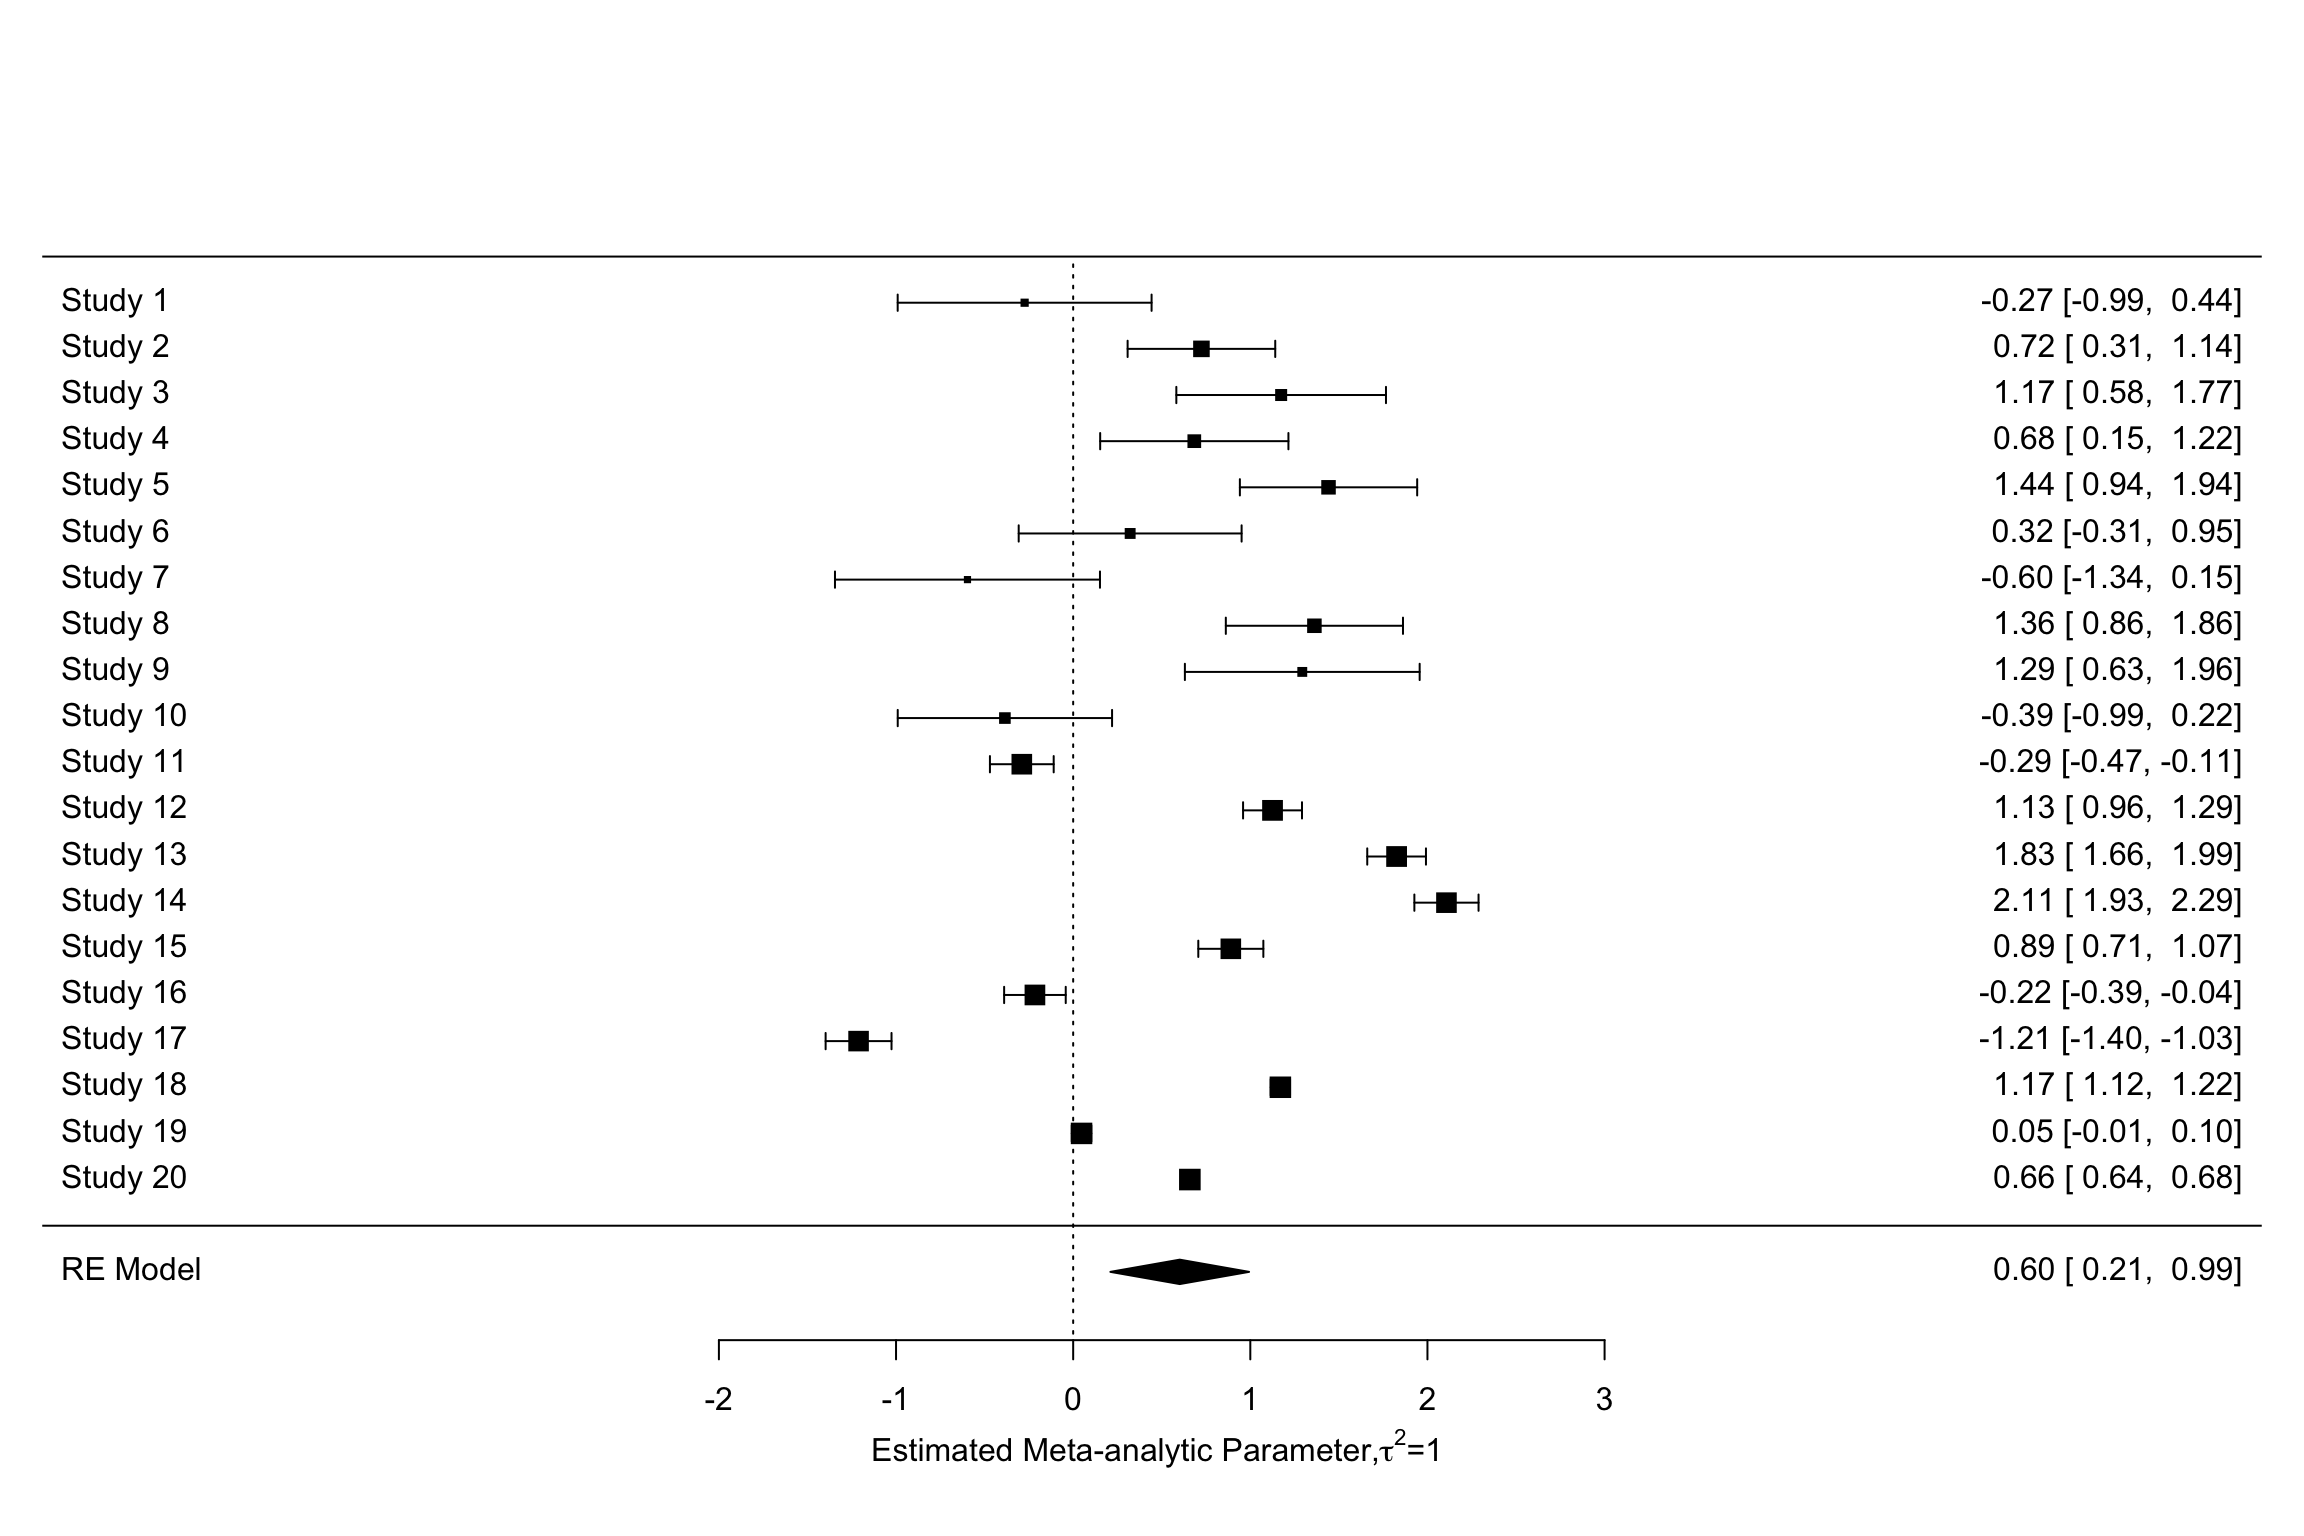
\includegraphics[width=0.33\linewidth]{STCI_files/figure-latex/RERMAmetafor-3} }

}

\caption{Forest plots with random effects}\label{fig:RERMAmetafor}
\end{figure}

Another very nice and useful graphical presentation device is a radial
(or Galbraith) plot. It relates the invserse of the standard errors to
the effect sizes normalized by their standard errors. Each data point is
also related a radius by the line passing through the origin. The Radial
plot enables to visualize the noise in the dataset, and is especially
useful when comparing a fixed and a random effects estimator for the
same study.

\begin{Shaded}
\begin{Highlighting}[]
\NormalTok{meta.example.FE.theta.}\DecValTok{1}\NormalTok{ <-}\StringTok{ }\KeywordTok{rma}\NormalTok{(}\DataTypeTok{yi =}\NormalTok{ data.meta}\OperatorTok{$}\NormalTok{theta.}\DecValTok{1}\NormalTok{,}\DataTypeTok{vi=}\NormalTok{data.meta}\OperatorTok{$}\NormalTok{var.ES,}\DataTypeTok{method=}\StringTok{"FE"}\NormalTok{)}
\KeywordTok{radial}\NormalTok{(meta.example.FE.theta.}\DecValTok{1}\NormalTok{)}
\KeywordTok{radial}\NormalTok{(meta.example.RE.theta.}\DecValTok{1}\NormalTok{)}
\end{Highlighting}
\end{Shaded}

\begin{figure}[htbp]

{\centering \subfloat[Fixed effects\label{fig:Radial1}]{\includegraphics[width=0.5\linewidth]{STCI_files/figure-latex/Radial-1} }\subfloat[Random effects\label{fig:Radial2}]{\includegraphics[width=0.5\linewidth]{STCI_files/figure-latex/Radial-2} }

}

\caption{Radial plots with fixed and random effects $\tau^2=$ 0.25}\label{fig:Radial}
\end{figure}

Figure \ref{fig:Radial} shows how the mechanics of the fixed effects
estimator differs from the mechanics of the random effects one. In the
presence of treatment effect heterogeneity, the fixed effect estimator
faces two issues:

\begin{enumerate}
\def\labelenumi{\arabic{enumi}.}
\tightlist
\item
  It gives too much weight to very precise estimators. The random
  effects estimator undoes part of this importance by adding \(\tau^2\)
  to the weights of each observation.
\item
  It overestimates overall precision by ignoring the sampling variance
  stemming from treatment effect heterogeneity across sites. The random
  effects estimator corrects for that by estimating \(\tau^2\) and
  adding it to the estimate of the total variance of the treatment
  effect.
\end{enumerate}

\BeginKnitrBlock{example}
\protect\hypertarget{exm:unnamed-chunk-140}{}{\label{exm:unnamed-chunk-140}
}Let's see how big a difference using random versus fixed effects does
to the estimation of treatment effects. Let's plot the two forest plots
for the example with \(\tau=\) \texttt{r\ tau{[}{[}1{]}{]}\^{}2}.
\EndKnitrBlock{example}

\begin{Shaded}
\begin{Highlighting}[]
\KeywordTok{forest}\NormalTok{(meta.example.FE.theta.}\DecValTok{1}\NormalTok{,}\DataTypeTok{slab =} \KeywordTok{paste}\NormalTok{(}\StringTok{'Study'}\NormalTok{,data.meta}\OperatorTok{$}\NormalTok{id,}\DataTypeTok{sep=}\StringTok{' '}\NormalTok{),}\DataTypeTok{xlab=}\StringTok{'Estimated Meta-analytic Parameter'}\NormalTok{)}
\KeywordTok{forest}\NormalTok{(meta.example.RE.theta.}\DecValTok{1}\NormalTok{,}\DataTypeTok{slab =} \KeywordTok{paste}\NormalTok{(}\StringTok{'Study'}\NormalTok{,data.meta}\OperatorTok{$}\NormalTok{id,}\DataTypeTok{sep=}\StringTok{' '}\NormalTok{),}\DataTypeTok{xlab=}\StringTok{'Estimated Meta-analytic Parameter'}\NormalTok{)}
\end{Highlighting}
\end{Shaded}

\begin{figure}[htbp]

{\centering \subfloat[Fixed effects\label{fig:FEvsRE1}]{\includegraphics[width=0.5\linewidth]{STCI_files/figure-latex/FEvsRE-1} }\subfloat[Random effects\label{fig:FEvsRE2}]{\includegraphics[width=0.5\linewidth]{STCI_files/figure-latex/FEvsRE-2} }

}

\caption{Fixed vs random effects with $\tau^2=$ 0.25}\label{fig:FEvsRE}
\end{figure}

Figure \ref{fig:FEvsRE} clearly shows that the inclusion of \(\tau^2\)
in the weights and precision estimates makes a huge difference to the
meta-analytic estimate. The fixed effects estimator yields an estimate
of our treatment effect of 0.3 \(\pm\) 0.02. The random effects
estimator yields an estimate of our treatment effect of 0.13 \(\pm\)
0.23. With \(\tau^2=\) 1, the random effects estimator yields an
estimate of our treatment effect of 0.6 \(\pm\) 0.39. Remember that the
true effect size of our treatment is 0.2. With \(\tau^2=\) 1, the random
effects estimator barely contains the truth in its 95 \(\%\) confidence
interval.

\subsection{Meta-regression}\label{meta-regression}

\subsection{Why vote-counting does not
work}\label{why-vote-counting-does-not-work}

\section{Publication bias}\label{publication-bias}

\subsection{Sources of publication
bias}\label{sources-of-publication-bias}

\subsection{Detecting and correcting for publication
bias}\label{detecting-and-correcting-for-publication-bias}

\subsubsection{P-curving}\label{p-curving}

\subsubsection{PET-PEESE}\label{pet-peese}

\subsubsection{Kasy and Andrews
approach}\label{kasy-and-andrews-approach}

\subsubsection{Last approach}\label{last-approach}

\subsection{Vote counting and publication
bias}\label{vote-counting-and-publication-bias}

\subsection{The value of a statistically significant
result}\label{the-value-of-a-statistically-significant-result}

\chapter{Bounds}\label{Bounds}

\appendix


\chapter{Proofs}\label{proofs}

\section{Proofs of results in Chapter
\ref{FPSI}}\label{proofs-of-results-in-chapter-reffpsi}

\subsection{Proof of Theorem \ref{thm:uppsampnoise}}\label{proofcheb}

In order to use Theorem \ref{thm:cheb} for studying the behavior of
\(\hat{\Delta^Y_{WW}}\), we have to prove that it is unbiased and we
have to compute \(\var{\hat{\Delta^Y_{WW}}}\). Let's first prove that
the \(WW\) estimator is an unbiased estimator of \(TT\):

\BeginKnitrBlock{lemma}[Unbiasedness of $\hat{\Delta^Y_{WW}}$]
\protect\hypertarget{lem:unbiasww}{}{\label{lem:unbiasww}
\iffalse (Unbiasedness of \(\hat{\Delta^Y_{WW}}\)) \fi{} }Under
Assumptions \ref{def:noselb}, \ref{def:fullrank} and \ref{def:iid},

\begin{align*}
\esp{\hat{\Delta^Y_{WW}}}& = \Delta^Y_{TT}.
\end{align*}
\EndKnitrBlock{lemma}

\BeginKnitrBlock{proof}
\iffalse{} {Proof. } \fi{}In order to prove Lemma \ref{lem:unbiasww}, we
are going to use a trick. We are going to compute the expectation of the
\(WW\) estimator conditional on a given treatment allocation. Because
the resulting estimate is independent of treatment allocation, we will
have our proof. This trick simplifies derivations a lot and is really
natural: think first of all the samples with the same treatment
allocation, then average your results over all possible treatment
allocations.

\begin{align*}
\esp{\hat{\Delta^Y_{WW}}} & = \esp{\esp{\hat{\Delta^Y_{WW}}|\mathbf{D}}}\\
                          & = \esp{\esp{\frac{1}{\sum_{i=1}^N D_i}\sum_{i=1}^N Y_iD_i-\frac{1}{\sum_{i=1}^N (1-D_i)}\sum_{i=1}^N Y_i(1-D_i)|\mathbf{D}}}\\
                          & = \esp{\esp{\frac{1}{\sum_{i=1}^N D_i}\sum_{i=1}^N Y_iD_i|\mathbf{D}}-\esp{\frac{1}{\sum_{i=1}^N (1-D_i)}\sum_{i=1}^N Y_i(1-D_i)|\mathbf{D}}}\\
                          & = \esp{\frac{1}{\sum_{i=1}^N D_i}\esp{\sum_{i=1}^N Y_iD_i|\mathbf{D}}-\frac{1}{\sum_{i=1}^N (1-D_i)}\esp{\sum_{i=1}^N Y_i(1-D_i)|\mathbf{D}}}\\
                          & = \esp{\frac{1}{\sum_{i=1}^N D_i}\sum_{i=1}^N \esp{Y_iD_i|\mathbf{D}}-\frac{1}{\sum_{i=1}^N (1-D_i)}\sum_{i=1}^N \esp{Y_i(1-D_i)|\mathbf{D}}}\\
                          & = \esp{\frac{1}{\sum_{i=1}^N D_i}\sum_{i=1}^N \esp{Y_iD_i|D_i}-\frac{1}{\sum_{i=1}^N (1-D_i)}\sum_{i=1}^N \esp{Y_i(1-D_i)|D_i}}\\
                          & = \esp{\frac{1}{\sum_{i=1}^N D_i}\sum_{i=1}^N D_i\esp{Y_i|D_i=1}-\frac{1}{\sum_{i=1}^N (1-D_i)}\sum_{i=1}^N(1-D_i)\esp{Y_i|D_i=0}}\\
                          & = \esp{\frac{\sum_{i=1}^N D_i}{\sum_{i=1}^N D_i}\esp{Y_i|D_i=1}-\frac{\sum_{i=1}^N(1-D_i)}{\sum_{i=1}^N (1-D_i)}\esp{Y_i|D_i=0}}\\
                          & = \esp{\esp{Y_i|D_i=1}-\esp{Y_i|D_i=0}}\\
                          & = \esp{Y_i|D_i=1}-\esp{Y_i|D_i=0} \\
                          & = \Delta^Y_{TT}.
\end{align*}

The first equality uses the Law of Iterated Expectations (LIE). The
second and fourth equalities use the linearity of conditional
expectations. The third equality uses the fact that, conditional on
\(\mathbf{D}\), the number of treated and untreated is a constant. The
fifth equality uses Assumption \ref{def:iid}. The sixth equality uses
the fact that
\(\esp{Y_iD_i|D_i}=D_i\esp{Y_i*1|D_i=1}+(1-D_i)\esp{Y_i*0|D_i=0}\). The
seventh and ninth equalities use the fact that \(\esp{Y_i|D_i=1}\) is a
constant. The last equality uses Assumption \ref{def:noselb}.
\EndKnitrBlock{proof}

Let's now compute the variance of the \(WW\) estimator:

\BeginKnitrBlock{lemma}[Variance of $\hat{\Delta^Y_{WW}}$]
\protect\hypertarget{lem:varww}{}{\label{lem:varww} \iffalse (Variance of
\(\hat{\Delta^Y_{WW}}\)) \fi{} }Under Assumptions \ref{def:noselb},
\ref{def:fullrank} and \ref{def:iid},

\begin{align*}
\var{{\hat{\Delta^Y_{WW}}}} & = \frac{1-(1-\Pr(D_i=1))^N}{N\Pr(D_i=1)}\var{Y_i^1|D_i=1}+\frac{1-\Pr(D_i=1)^N}{N(1-\Pr(D_i=1))}\var{Y_i^0|D_i=0}.
\end{align*}
\EndKnitrBlock{lemma}

\BeginKnitrBlock{proof}
\iffalse{} {Proof. } \fi{}Same trick as before, but now using the Law of
Total Variance (LTV):

\begin{align*}
\var{{\hat{\Delta^Y_{WW}}}} & = \esp{\var{\hat{\Delta^Y_{WW}}|\mathbf{D}}}+\var{\esp{\hat{\Delta^Y_{WW}}|\mathbf{D}}}\\
                            & = \esp{\var{\frac{1}{\sum_{i=1}^N D_i}\sum_{i=1}^N Y_iD_i-\frac{1}{\sum_{i=1}^N (1-D_i)}\sum_{i=1}^N Y_i(1-D_i)|\mathbf{D}}} \\
                            & = \esp{\var{\frac{1}{\sum_{i=1}^N D_i}\sum_{i=1}^N Y_iD_i|\mathbf{D}}}+\esp{\var{\frac{1}{\sum_{i=1}^N (1-D_i)}\sum_{i=1}^N Y_i(1-D_i)|\mathbf{D}}}\\
                            & \phantom{=}+\esp{\cov{\frac{1}{\sum_{i=1}^N D_i}\sum_{i=1}^N Y_iD_i,\frac{1}{\sum_{i=1}^N (1-D_i)}\sum_{i=1}^N Y_i(1-D_i)|\mathbf{D}}} \\
                            & = \esp{\frac{1}{(\sum_{i=1}^N D_i)^2}\var{\sum_{i=1}^N Y_iD_i|\mathbf{D}}}+\esp{\frac{1}{(\sum_{i=1}^N (1-D_i))^2}\var{\sum_{i=1}^N Y_i(1-D_i)|\mathbf{D}}} \\
                            & = \esp{\frac{1}{(\sum_{i=1}^N D_i)^2}\var{\sum_{i=1}^N Y_iD_i|D_i}}+\esp{\frac{1}{(\sum_{i=1}^N (1-D_i))^2}\var{\sum_{i=1}^N Y_i(1-D_i)|D_i}} \\
                            & = \esp{\frac{1}{(\sum_{i=1}^N D_i)^2}\sum_{i=1}^ND_i\var{Y_i|D_i=1}}+\esp{\frac{1}{(\sum_{i=1}^N (1-D_i))^2}\sum_{i=1}^N(1-D_i)\var{Y_i|D_i=0}} \\
                            & = \var{Y_i|D_i=1}\esp{\frac{1}{\sum_{i=1}^N D_i}}+\var{Y_i|D_i=0}\esp{\frac{1}{\sum_{i=1}^N (1-D_i)}} \\
                            & = \frac{1-(1-\Pr(D_i=1))^N}{N\Pr(D_i=1)}\var{Y_i^1|D_i=1}+\frac{1-\Pr(D_i=1)^N}{N(1-\Pr(D_i=1))}\var{Y_i^0|D_i=0}.
\end{align*}

The first equality stems from the LTV. The second and third equalities
stems from the definition of the \(WW\) estimator and of the variance of
a sum of random variables. The fourth equality stems from Assumption
\ref{def:iid}, which means that the covariance across observations is
zero, and from the formula for a variance of a random variable
multiplied by a constant. The fifth and sixth equalities stems from
Assumption \ref{def:iid} and from
\(\var{Y_iD_i|D_i}=D_i\var{Y_i*1|D_i=1}+(1-D_i)\var{Y_i*0|D_i=0}\). The
seventh equality stems from \(\var{Y_i|D_i=1}\) and \(\var{Y_i|D_i=0}\)
being constant. The last equality stems from the formula for the
expectation of the inverse of a sum of Bernoulli random variables with
at least one of them taking value one which is the case under Assumption
\ref{def:fullrank}.
\EndKnitrBlock{proof}

Using Theorem \ref{thm:cheb}, we have:

\begin{align*}
2\epsilon & \leq 2\sqrt{\frac{1}{N(1-\delta)}\left(\frac{1-(1-\Pr(D_i=1))^N}{\Pr(D_i=1)}\var{Y_i^1|D_i=1}+\frac{1-\Pr(D_i=1)^N}{(1-\Pr(D_i=1))}\var{Y_i^0|D_i=0}\right)}\\
          & \leq 2\sqrt{\frac{1}{N(1-\delta)}\left(\frac{\var{Y_i^1|D_i=1}}{\Pr(D_i=1)}+\frac{\var{Y_i^0|D_i=0}}{(1-\Pr(D_i=1))}\right)},
\end{align*}

where the second equality stems from the fact that
\(\frac{(1-\Pr(D_i=1))^N}{\Pr(D_i=1)}\var{Y_i^1|D_i=1}+\frac{\Pr(D_i=1)^N}{(1-\Pr(D_i=1))}\var{Y_i^0|D_i=0}\geq0\).
This proves the result.

\subsection{Proof of Theorem \ref{thm:asympnoiseWW}}\label{proofCLT}

Before proving Theorem \ref{thm:asympnoiseWW}, let me state a very
useful result: \(\hat{WW}\) can be computed using OLS:

\BeginKnitrBlock{lemma}[WW is OLS]
\protect\hypertarget{lem:WWOLS}{}{\label{lem:WWOLS} \iffalse (WW is OLS)
\fi{} }Under Assumption \ref{def:fullrank}, the OLS coefficient
\(\beta\) in the following regression:

\begin{align*}
        Y_i &  = \alpha +  \beta D_i + U_i
    \end{align*}

is the WW estimator:

\begin{align*}
\hat{\beta}_{OLS} & = \frac{\frac{1}{N}\sum_{i=1}^N\left(Y_i-\frac{1}{N}\sum_{i=1}^NY_i\right)\left(D_i-\frac{1}{N}\sum_{i=1}^ND_i\right)}{\frac{1}{N}\sum_{i=1}^N\left(D_i-\frac{1}{N}\sum_{i=1}^ND_i\right)^2} \\
                                & = \hat{\Delta^Y_{WW}}.
\end{align*}
\EndKnitrBlock{lemma}

\BeginKnitrBlock{proof}
\iffalse{} {Proof. } \fi{}In matrix notation, we have:

\begin{align*}
  \underbrace{\left(\begin{array}{c}  Y_1 \\    \vdots \\   Y_N \end{array}\right)}_{Y} & = 
  \underbrace{\left(\begin{array}{cc}   1 & D_1\\   \vdots & \vdots\\   1 & D_N\end{array}\right)}_{X}
  \underbrace{\left(\begin{array}{c}    \alpha \\   \beta \end{array}\right)}_{\Theta}+
  \underbrace{\left(\begin{array}{c}    U_1 \\  \vdots \\   U_N \end{array}\right)}_{U}
\end{align*}

The OLS estimator is:

\begin{align*}
    \hat{\Theta}_{OLS} &  = (X'X)^{-1}X'Y
\end{align*}

Under the Full Rank Assumption, \(X'X\) is invertible and we have:

\begin{align*}
(X'X)^{-1} &  = \left(\begin{array}{cc} N & \sum_{i=1}^ND_i \\ \sum_{i=1}^ND_i & \sum_{i=1}^ND_i^2 \end{array}\right)^{-1} \\
                & = \frac{1}{N\sum_{i=1}^ND_i^2-\left(\sum_{i=1}^ND_i\right)^2}\left(\begin{array}{cc} \sum_{i=1}^ND_i^2 & -\sum_{i=1}^ND_i \\ -\sum_{i=1}^ND_i & N \end{array}\right)
\end{align*}

For simplicity, I omit the summation index:

\begin{align*}
  \hat{\Theta}_{OLS} &  = \frac{1}{N\sum D_i^2-\left(\sum D_i\right)^2}
                          \left(\begin{array}{cc} \sum D_i^2 & -\sum D_i \\ -\sum D_i & N \end{array}\right)
                          \left(\begin{array}{c} \sum Y_i \\  \sum Y_iD_i \end{array}\right) \\
                    & = \frac{1}{N\sum D_i^2-\left(\sum D_i\right)^2}
                        \left(\begin{array}{c} \sum D_i^2\sum Y_i-\sum D_i\sum_{i=1}^NY_iD_i \\
                                              -\sum D_i\sum Y_i+ N\sum Y_iD_i \end{array}\right) \\
\end{align*}

Using \(D_i^2=D_i\), we have:

\begin{align*}
  \hat{\Theta}_{OLS} &  =  \left(\begin{array}{c} 
          \frac{\left(\sum D_i\right)\left(\sum Y_i-\sum Y_iD_i\right)}{\left(\sum D_i\right)\left(N-\sum D_i\right)} \\
          \frac{N\sum Y_iD_i-\sum D_i\sum Y_i}{N\sum D_i-\left(\sum D_i\right)^2} 
                            \end{array}\right) 
                        =     \left(\begin{array}{c} 
          \frac{\sum (Y_iD_i+Y_i(1-D_i))-\sum Y_iD_i}{\sum(1-D_i)} \\
          \frac{N^2}{N^2}\frac{\frac{1}{N}\sum Y_iD_i-\frac{1}{N}\sum D_i\frac{1}{N}\sum Y_i+\frac{1}{N}\sum D_i\frac{1}{N}\sum Y_i-\frac{1}{N}\sum D_i\frac{1}{N}\sum Y_i}{\frac{1}{N}\sum D_i-2\left(\frac{1}{N}\sum D_i\right)^2+\left(\frac{1}{N}\sum D_i\right)^2} 
                            \end{array}\right) \\
                      &  =     \left(\begin{array}{c} 
          \frac{\sum Y_i(1-D_i)}{\sum(1-D_i)} \\
          \frac{\frac{1}{N}\sum \left(Y_iD_i-D_i\frac{1}{N}\sum Y_i-Y_i\frac{1}{N}\sum D_i+\frac{1}{N}\sum D_i\frac{1}{N}\sum Y_i\right)}{\frac{1}{N}\sum\left(D_i-2D_i\frac{1}{N}\sum D_i+\left(\frac{1}{N}\sum D_i\right)^2\right)} 
                            \end{array}\right) 
                      =     \left(\begin{array}{c} 
          \frac{\sum Y_i(1-D_i)}{\sum(1-D_i)} \\
    \frac{\frac{1}{N}\sum\left(Y_i-\frac{1}{N}\sum Y_i\right)\left(D_i-\frac{1}{N}\sum D_i\right)}{\frac{1}{N}\sum \left(D_i-\frac{1}{N}\sum D_i\right)^2} 
                            \end{array}\right), 
\end{align*}

which proves the first part of the lemma. Now for the second part of the
lemma:

\begin{align*}
  \hat{\beta}_{OLS} &  = \frac{\sum Y_iD_i-\frac{1}{N}\sum D_i\sum Y_i}{\sum D_i\left(1-\frac{1}{N}\sum D_i\right)}
                       = \frac{\sum Y_iD_i-\frac{1}{N}\sum D_i\sum\left(Y_iD_i+(1-D_i)Y_i\right)}{\sum D_i\left(1-\frac{1}{N}\sum D_i\right)}\\
                    &  = \frac{\sum Y_iD_i\left(1-\frac{1}{N}\sum D_i\right)-\frac{1}{N}\sum D_i\sum(1-D_i)Y_i}{\sum D_i\left(1-\frac{1}{N}\sum D_i\right)}\\
                    &  = \frac{\sum Y_iD_i}{\sum D_i}-\frac{\frac{1}{N}\sum(1-D_i)Y_i}{\left(1-\frac{1}{N}\sum D_i\right)}\\
                    &  = \frac{\sum Y_iD_i}{\sum D_i}-\frac{\frac{1}{N}\sum(1-D_i)Y_i}{\frac{1}{N}\sum\left(1-D_i\right)}\\
                     &  = \frac{\sum Y_iD_i}{\sum D_i}-\frac{\sum(1-D_i)Y_i}{\sum\left(1-D_i\right)}\\
                     & = \hat{\Delta^Y_{WW}},
\end{align*}

which proves the result.
\EndKnitrBlock{proof}

Now, let me state the most important lemma behind the result in Theorem
\ref{thm:asympnoiseWW}:

\BeginKnitrBlock{lemma}[Asymptotic Distribution of the OLS Estimator]
\protect\hypertarget{lem:asympOLS}{}{\label{lem:asympOLS}
\iffalse (Asymptotic Distribution of the OLS Estimator) \fi{} }Under
Assumptions \ref{def:noselb}, \ref{def:fullrank}, \ref{def:iid} and
\ref{def:finitevar}, we have:

\begin{align*}
  \sqrt{N}(\hat{\Theta}_{OLS}-\Theta) &  \stackrel{d}{\rightarrow}
  \mathcal{N}\left(\begin{array}{c} 0\\ 0\end{array},
  \sigma_{XX}^{-1}\mathbf{V_{xu}}\sigma_{XX}^{-1}\right), 
\end{align*}

with

\begin{align*}
\sigma_{XX}^{-1}& = \left(\begin{array}{cc} \frac{\Pr(D_i=1)}{\Pr(D_i=1)(1-\Pr(D_i=1))} & -\frac{\Pr(D_i=1)}{\Pr(D_i=1)(1-\Pr(D_i=1))}\\
                                          -\frac{\Pr(D_i=1)}{\Pr(D_i=1)(1-\Pr(D_i=1))} & \frac{1}{\Pr(D_i=1)(1-\Pr(D_i=1))} 
                          \end{array}\right)\\
\mathbf{V_{xu}}&= \esp{U_i^2\left(\begin{array}{cc}  1 & D_i\\  D_i & D_i\end{array}\right)}                        
\end{align*}
\EndKnitrBlock{lemma}

\BeginKnitrBlock{proof}
\iffalse{} {Proof. } \fi{}

\begin{align*}
\sqrt{N}(\hat{\Theta}_{OLS}-\Theta) & = \sqrt{N}((X'X)^{-1}X'Y-\Theta) \\
                                    & = \sqrt{N}((X'X)^{-1}X'(X\Theta+U)-\Theta) \\
                                    & = \sqrt{N}((X'X)^{-1}X'X\Theta+(X'X)^{-1}X'U)-\Theta) \\
                                    & = \sqrt{N}(X'X)^{-1}X'U \\
                                    & = N(X'X)^{-1}\frac{\sqrt{N}}{N}X'U
\end{align*}

Using Slutsky's Theorem, we can study both terms separately. Slutsky's
Theorem states that if \(Y_N\stackrel{d}{\rightarrow}y\) and
\(\text{plim}(X_N)=x\), then:

\begin{enumerate}
\def\labelenumi{\arabic{enumi}.}
\tightlist
\item
  \(X_N+Y_N\stackrel{d}{\rightarrow}x+y\)
\item
  \(X_NY_N\stackrel{d}{\rightarrow}xy\)
\item
  \(\frac{Y_N}{X_N}\stackrel{d}{\rightarrow}\frac{x}{y}\) if \(x\neq0\)
\end{enumerate}

Using this theorem, we have:

\begin{align*}
\sqrt{N}(\hat{\Theta}_{OLS}-\Theta) & \stackrel{d}{\rightarrow} \sigma_{XX}^{-1}xu,
\end{align*}

Where \(\sigma_{XX}^{-1}\) is a matrix of constants and \(xu\) is a
random variable.

Let's begin with \(\frac{\sqrt{N}}{N}X'U\stackrel{d}{\rightarrow}xu\):

\begin{align*}
\frac{\sqrt{N}}{N}X'U & = \sqrt{N}\left(\begin{array}{c}  \frac{1}{N}\sum^{i=1}_{N}U_i\\  \frac{1}{N}\sum^{i=1}_{N}D_iU_i\end{array}\right)
\end{align*}

In order to determine the asymptotic distribution of
\(\frac{\sqrt{N}}{N}X'U\), we are going to use the vector version of the
CLT:

If \(X_i\) and \(Y_i\) are two i.i.d. random variables with finite first
and second moments, we have:

\begin{align*}
    \sqrt{N}
  \left(
      \begin{array}{c}  
       \frac{1}{N}\sum_{i=1}^NX_i-\esp{X_i}\\   
       \frac{1}{N}\sum_{i=1}^NY_i-\esp{Y_i}
       \end{array}
     \right) 
      &
  \stackrel{d}{\rightarrow}
  \mathcal{N}
  \left(
    \begin{array}{c}    
    0\\
    0
    \end{array},
  \mathbf{V}
  \right),
\end{align*}

where \(\mathbf{V}\) is the population covariance matrix of \(X_i\) and
\(Y_i\).

We know that, under Assumption \ref{def:noselb}, both random variables
have mean zero:

\begin{align*}
\esp{U_i}& = \esp{U_i|D_i=1}\Pr(D_i=1)+\esp{U_i|D_i=0}\Pr(D_i=0)=0 \\
\esp{U_iD_i}& = \esp{U_i|D_i=1}\Pr(D_i=1)=0
\end{align*}

Their covariance matrix \(\mathbf{V_{xu}}\) can be computed as follows:

\begin{align*}
\mathbf{V_{xu}} & = \esp{\left(\begin{array}{c}  U_i\\  UiD_i\end{array}\right)\left(\begin{array}{cc}  U_i&    UiD_i\end{array}\right)}
                  - \esp{\left(\begin{array}{c} U_i\\   UiD_i\end{array}\right)}\esp{\left(\begin{array}{cc}    U_i&    UiD_i\end{array}\right)}\\
                & = \esp{\left(\begin{array}{cc}    U_i^2 & U_i^2D_i\\  Ui^2D_i & U_i^2D_i^2\end{array}\right)} 
                  = \esp{U_i^2\left(\begin{array}{cc}   1 & D_i\\   D_i & D_i^2\end{array}\right)} 
                  = \esp{U_i^2\left(\begin{array}{cc}   1 & D_i\\   D_i & D_i\end{array}\right)} 
\end{align*}

Using the Vector CLT, we have that
\(\frac{\sqrt{N}}{N}X'U\stackrel{d}{\rightarrow}\mathcal{N}\left(\begin{array}{c} 0\\ 0\end{array},\mathbf{V_{xu}}\right)\).

Let's show now that \(\plims N(X'X)^{-1}=\sigma_{XX}^{-1}\):

\begin{align*}
N(X'X)^{-1} & = \frac{N}{N\sum_{i=1}^ND_i-\left(\sum_{i=1}^ND_i\right)^2}
                \left(\begin{array}{cc} \sum_{i=1}^ND_i & -\sum_{i=1}^ND_i \\ -\sum_{i=1}^ND_i & N \end{array}\right) \\
            & = \frac{1}{N}\frac{1}{\frac{1}{N}\sum_{i=1}^ND_i-\left(\frac{1}{N}\sum_{i=1}^ND_i\right)^2}
                \left(\begin{array}{cc} \sum_{i=1}^ND_i & -\sum_{i=1}^ND_i \\ -\sum_{i=1}^ND_i & N \end{array}\right)\\
            & = \frac{1}{\frac{1}{N}\sum_{i=1}^ND_i-\left(\frac{1}{N}\sum_{i=1}^ND_i\right)^2}
                \left(\begin{array}{cc} \frac{1}{N}\sum_{i=1}^ND_i & -\frac{1}{N}\sum_{i=1}^ND_i \\ -\frac{1}{N}\sum_{i=1}^ND_i & 1 \end{array}\right)\\
\plims N(X'X)^{-1} & = \frac{1}{\plims\frac{1}{N}\sum_{i=1}^ND_i-\left(\plims\frac{1}{N}\sum_{i=1}^ND_i\right)^2}
                \left(\begin{array}{cc} \plims\frac{1}{N}\sum_{i=1}^ND_i & -\plims\frac{1}{N}\sum_{i=1}^ND_i \\ -\plims\frac{1}{N}\sum_{i=1}^ND_i & 1 \end{array}\right)\\
                  & = \frac{1}{\Pr(D_i=1)-\Pr(D_i=1)^2}
                \left(\begin{array}{cc} \Pr(D_i=1) & -\Pr(D_i=1) \\ -\Pr(D_i=1) & 1 \end{array}\right)\\
                 & = \sigma_{XX}^{-1}
\end{align*}

The fourth equality uses Slutsky's Theorem. The fifth equality uses the
Law of Large Numbers (LLN): if \(Y_i\) are i.i.d. variables with finite
first and second moments,
\(\plim{N}\frac{1}{N}\sum_{i=1}^NY_i = \esp{Y_i}\).

In order to complete the proof, we have to use the Delta Method Theorem.
This theorem states that:

\begin{gather*}
  \sqrt{N}(\begin{array}{c} \bar{X}_N-\esp{X_i}\\   \bar{Y}_N-\esp{Y_i}\end{array})  \stackrel{d}{\rightarrow}\mathcal{N}(\begin{array}{c}  0\\ 0\end{array},\mathbf{V}) \\
\Rightarrow \sqrt{N}(g(\bar{X}_N,\bar{Y}_N)-g(\esp{X_i},\esp{Y_i})  \stackrel{d}{\rightarrow}\mathcal{N}(0,G'\mathbf{V}G)
\end{gather*}

where \(G(u)=\partder{g(u)}{u}\) and \(G=G(\esp{X_i},\esp{Y_i})\).

In our case, \(g(xu)=\sigma_{XX}^{-1}xu\), so
\(G(xu)=\sigma_{XX}^{-1}\). The results follows from that and from the
symmetry of \(\sigma_{XX}^{-1}\).
\EndKnitrBlock{proof}

A last lemma uses the previous result to derive the asymptotic
distribution of \(\hat{WW}\):

\BeginKnitrBlock{lemma}[Asymptotic Distribution of $\hat{WW}$]
\protect\hypertarget{lem:asymWW}{}{\label{lem:asymWW} \iffalse (Asymptotic
Distribution of \(\hat{WW}\)) \fi{} }Under Assumptions \ref{def:noselb},
\ref{def:fullrank}, \ref{def:iid} and \ref{def:finitevar}, we have:

\begin{align*}
  \sqrt{N}(\hat{\Delta^Y_{WW}}-\Delta^Y_{TT}) &  \stackrel{d}{\rightarrow}
  \mathcal{N}\left(0,\frac{\var{Y_i^1|D_i=1}}{\Pr(D_i=1)}+\frac{\var{Y_i^0|D_i=0}}{1-\Pr(D_i=1)}\right).
\end{align*}
\EndKnitrBlock{lemma}

\BeginKnitrBlock{proof}
\iffalse{} {Proof. } \fi{}In order to derive the asymptotic distribution
of WW, I use first Lemma \ref{lem:WWOLS} which implies that the
asymptotic distribution of WW is the same as that of
\(\hat{\beta}_{OLS}\). Now, from Lemma \ref{lem:asympOLS}, we know that
\(\sqrt{N}(\hat{\beta}_{OLS}-\beta)\stackrel{d}{\rightarrow}\mathcal{N}(0,\sigma^2_{\beta})\),
where \(\sigma^2_{\beta}\) is the lower diagonal term of
\(\sigma_{XX}^{-1}\mathbf{V_{xu}}\sigma_{XX}^{-1}\). Using the
convention \(p=\Pr(D_i=1)\), we have:

\begin{align*}
\sigma_{XX}^{-1}\mathbf{V_{xu}}\sigma_{XX}^{-1} 
                  & = \left(\begin{array}{cc}  
                                          \frac{p}{p(1-p)} & -\frac{p}{p(1-p)}\\
                                          -\frac{p}{p(1-p)} & \frac{1}{p(1-p)} 
                          \end{array}\right)
                          \esp{U_i^2\left(\begin{array}{cc}  1 & D_i\\  D_i & D_i\end{array}\right)}        
                          \left(\begin{array}{cc}  
                                          \frac{p}{p(1-p)} & -\frac{p}{p(1-p)}\\
                                          -\frac{p}{p(1-p)} & \frac{1}{p(1-p)} 
                          \end{array}\right)\\
                  & = \frac{1}{(p(1-p))^2}
                          \left(\begin{array}{cc}  
                                          p\esp{U_i^2}-p\esp{U_i^2D_i} & p\esp{U_i^2D_i}-p\esp{U_i^2D_i}\\
                                          -p\esp{U_i^2}+\esp{U_i^2D_i} &  -p\esp{U_i^2D_i}+\esp{U_i^2D_i}
                          \end{array}\right)
                         \left(\begin{array}{cc}  
                                          p & -p\\
                                          -p & 1 
                          \end{array}\right)\\
                 & = \frac{1}{(p(1-p))^2}
                          \left(\begin{array}{cc}  
                                          p^2(\esp{U_i^2}-\esp{U_i^2D_i}) & p^2(\esp{U_i^2D_i}-\esp{U_i^2})\\
                                          p^2(\esp{U_i^2D_i}-\esp{U_i^2}) &  p^2\esp{U_i^2}+(1-2p)\esp{U_i^2D_i}
                          \end{array}\right)
 \end{align*}

The final result comes from the fact that:

\begin{align*}
\esp{U_i^2} & = \esp{U_i^2|D_i=1}p + (1-p)\esp{U_i^2|D_i=0}\\
            & = p\var{Y_i^1|D_i=1}+(1-p)\var{Y_i^0|D_i=0} \\
\esp{U_i^2D_i}  & = \esp{U_i^2|D_i=1}p  \\
                & = p\var{Y_i^1|D_i=1}.
 \end{align*}

As a consequence:

\begin{align*}
\sigma^2_{\beta} &= \frac{1}{(p(1-p))^2}\left(\var{Y_i^1|D_i=1}p(p^2-2p+1) + p^2(1-p)\var{Y_i^0|D_i=0}\right) \\
                  &= \frac{1}{(p(1-p))^2}\left(\var{Y_i^1|D_i=1}p(1-p)^2 + p^2(1-p)\var{Y_i^0|D_i=0}\right)\\
                  & = \frac{\var{Y_i^1|D_i=1}}{p}+\frac{\var{Y_i^0|D_i=0}}{1-p}.
 \end{align*}
\EndKnitrBlock{proof}

Using the previous lemma, we can now approximate the confidence level of
\(\hat{WW}\):

\begin{align*}
\Pr&(|\hat{\Delta^Y_{WW}}-\Delta^Y_{TT}|\leq\epsilon) = \Pr(-\epsilon\leq\hat{\Delta^Y_{WW}}-\Delta^Y_{TT}\leq\epsilon) \\
& = \Pr\left(-\frac{\epsilon}{\frac{1}{\sqrt{N}}\sqrt{\frac{\var{Y_i^1|D_i=1}}{\Pr(D_i=1)}+\frac{\var{Y_i^0|D_i=0}}{1-\Pr(D_i=1)}}}\leq\frac{\hat{\Delta^Y_{WW}}-\Delta^Y_{TT}}{\frac{1}{\sqrt{N}}\sqrt{\frac{\var{Y_i^1|D_i=1}}{\Pr(D_i=1)}+\frac{\var{Y_i^0|D_i=0}}{1-\Pr(D_i=1)}}}\leq\frac{\epsilon}{\frac{1}{\sqrt{N}}\sqrt{\frac{\var{Y_i^1|D_i=1}}{\Pr(D_i=1)}+\frac{\var{Y_i^0|D_i=0}}{1-\Pr(D_i=1)}}}\right)\\
& \approx \Phi\left(\frac{\epsilon}{\frac{1}{\sqrt{N}}\sqrt{\frac{\var{Y_i^1|D_i=1}}{\Pr(D_i=1)}+\frac{\var{Y_i^0|D_i=0}}{1-\Pr(D_i=1)}}}\right)-
\Phi\left(-\frac{\epsilon}{\frac{1}{\sqrt{N}}\sqrt{\frac{\var{Y_i^1|D_i=1}}{\Pr(D_i=1)}+\frac{\var{Y_i^0|D_i=0}}{1-\Pr(D_i=1)}}}\right)\\
& = \Phi\left(\frac{\epsilon}{\frac{1}{\sqrt{N}}\sqrt{\frac{\var{Y_i^1|D_i=1}}{\Pr(D_i=1)}+\frac{\var{Y_i^0|D_i=0}}{1-\Pr(D_i=1)}}}\right)- 1 + \Phi\left(\frac{\epsilon}{\frac{1}{\sqrt{N}}\sqrt{\frac{\var{Y_i^1|D_i=1}}{\Pr(D_i=1)}+\frac{\var{Y_i^0|D_i=0}}{1-\Pr(D_i=1)}}}\right)\\
& = 2\Phi\left(\frac{\epsilon}{\frac{1}{\sqrt{N}}\sqrt{\frac{\var{Y_i^1|D_i=1}}{\Pr(D_i=1)}+\frac{\var{Y_i^0|D_i=0}}{1-\Pr(D_i=1)}}}\right)-1.
\end{align*}

As a consequence,

\begin{align*}
\delta & \approx 2\Phi\left(\frac{\epsilon}{\frac{1}{\sqrt{N}}\sqrt{\frac{\var{Y_i^1|D_i=1}}{\Pr(D_i=1)}+\frac{\var{Y_i^0|D_i=0}}{1-\Pr(D_i=1)}}}\right)-1.
\end{align*}

Hence the result.

\section{Proofs of results in Chapter
\ref{RCT}}\label{proofs-of-results-in-chapter-refrct}

\subsection{Proof of Theorem \ref{thm:IdentLATE}}\label{proofIdentLATE}

In order to prove the theorem, it is going to be very helpful to prove
the following lemma:

\BeginKnitrBlock{lemma}[Unconfounded Types]
\protect\hypertarget{lem:UnconfTypes}{}{\label{lem:UnconfTypes}
\iffalse (Unconfounded Types) \fi{} }Under Assumptions
\ref{def:RandEncouragValid} and \ref{def:IndepEncourag}, the types
\(T_i\) are independent of the allocation of the treatment:

\begin{align*}
(Y_i^{1,1},Y_i^{0,1},Y_i^{0,0},Y_i^{1,0},T_i)\Ind R_i|E_i=1.
\end{align*}
\EndKnitrBlock{lemma}

\BeginKnitrBlock{proof}
\iffalse{} {Proof. } \fi{}Lemma 4.2 in
\href{https://www.jstor.org/stable/2984718}{Dawid (1979)} shows that if
\(X\Ind Y|Z\) and \(U\) is a function of \(X\) then \(U\Ind Y|Z\). The
fact that \(T_i\) is a function of \((D_i^1,D^0_i)\) proves the result.
\EndKnitrBlock{proof}

The four sets defined by \(T_i\) are a partition of the sample space. As
a consequence, we have (ommitting the conditioning on \(E_i=1\) all
along for simplicity):

\begin{align*}
\esp{Y_i|R_i=1} & = \esp{Y_i|T_i=a,R_i=1}\Pr(T_i=a|R_i=1)\\
                & \phantom{=}+ \esp{Y_i|T_i=c,R_i=1}\Pr(T_i=c|R_i=1) \\
                            & \phantom{=} + \esp{Y_i|T_i=d,R_i=1}\Pr(T_i=d|R_i=1)\\
                            & \phantom{=} + \esp{Y_i|T_i=n,R_i=1}\Pr(T_i=n|R_i=1)\\
\esp{Y_i|R_i=0} & = \esp{Y_i|T_i=a,R_i=0}\Pr(T_i=a|R_i=0)\\
                & \phantom{=} + \esp{Y_i|T_i=c,R_i=0}\Pr(T_i=c|R_i=0) \\
                            & \phantom{=} + \esp{Y_i|T_i=d,R_i=0}\Pr(T_i=d|R_i=0)\\
                            & \phantom{=}+ \esp{Y_i|T_i=n,R_i=0}\Pr(T_i=n|R_i=0).
\end{align*}

Let's look at all these terms in turn:

\begin{align*}
  \esp{Y_i|T_i=a,R_i=1} & =   \esp{Y_i^{1,1}D_iR_i+Y_i^{1,0}D_i(1-R_i)+Y_i^{0,1}(1-D_i)R_i+Y_i^{0,0}(1-D_i)(1-R_i)|T_i=a,R_i=1} \\
   & =   \esp{Y_i^{1,1}(D^1_iR_i+D_i^0(1-R_i))R_i+Y_i^{0,1}(1-(D^1_iR_i+D_i^0(1-R_i)))R_i|T_i=a,R_i=1} \\
   & =   \esp{Y_i^{1,1}D^1_iR_i^2+Y_i^{0,1}(1-D^1_iR_i)R_i|D_i^1=D_i^0=1,R_i=1} \\
   & =   \esp{Y_i^{1,1}|T_i=a,R_i=1} \\
   & =   \esp{Y_i^{1,1}|T_i=a}, \\
\end{align*}

where the first equality uses Assumption \ref{def:RandEncouragValid},
the second equality uses the fact that \(R_i=1\) in the conditional
expectation and Assumption \ref{def:RandEncouragValid}, the third
equality uses the fact that \(R_i=1\), the fourth equality uses the fact
that \(T_i=a \Leftrightarrow D_i^1=D_i^0=1\) and the last equality uses
Lemma \ref{lem:UnconfTypes}.

Using a similar reasoning, we have:

\begin{align*}
  \esp{Y_i|T_i=c,R_i=1} & = \esp{Y_i^{1,1}|T_i=c} \\
  \esp{Y_i|T_i=d,R_i=1} & = \esp{Y_i^{0,1}|T_i=d} \\
  \esp{Y_i|T_i=n,R_i=1} & = \esp{Y_i^{0,1}|T_i=n} \\
  \esp{Y_i|T_i=a,R_i=0} & = \esp{Y_i^{1,0}|T_i=c} \\
  \esp{Y_i|T_i=c,R_i=0} & = \esp{Y_i^{0,0}|T_i=c} \\
  \esp{Y_i|T_i=d,R_i=0} & = \esp{Y_i^{1,0}|T_i=d} \\
  \esp{Y_i|T_i=n,R_i=0} & = \esp{Y_i^{0,0}|T_i=n}.
\end{align*}

Also, Lemma \ref{lem:UnconfTypes} implies that
\(\Pr(T_i=a|R_i)=\Pr(T_i=a)\), and the same is true for all other types.
As a consequence, we have:

\begin{align*}
\esp{Y_i|R_i=1} & = \esp{Y_i^{1,1}|T_i=a}\Pr(T_i=a)\\
                & \phantom{=} + \esp{Y_i^{1,1}|T_i=c}\Pr(T_i=c) \\
                            & \phantom{=} + \esp{Y_i^{0,1}|T_i=d}\Pr(T_i=d)\\
                            & \phantom{=} + \esp{Y_i^{0,1}|T_i=n}\Pr(T_i=n)\\
\esp{Y_i|R_i=0} & = \esp{Y_i^{1,0}|T_i=a}\Pr(T_i=a)\\
                & \phantom{=} + \esp{Y_i^{0,0}|T_i=c}\Pr(T_i=c) \\                      
                                & \phantom{=} + \esp{Y_i^{1,0}|T_i=d}\Pr(T_i=d)\\
                                & \phantom{=} + \esp{Y_i^{0,0}|T_i=n}\Pr(T_i=n).
\end{align*}

And thus:

\begin{align*}
\esp{Y_i|R_i=1}-\esp{Y_i|R_i=0} & = (\esp{Y_i^{1,1}|T_i=a}-\esp{Y_i^{1,0}|T_i=a})\Pr(T_i=a)\\
                                & \phantom{=}+ (\esp{Y_i^{1,1}|T_i=c}-\esp{Y_i^{0,0}|T_i=c})\Pr(T_i=c) \\
                                            & \phantom{=} - (\esp{Y_i^{1,0}|T_i=d}-\esp{Y_i^{0,1}|T_i=d})\Pr(T_i=d)\\
                                            & \phantom{=} + (\esp{Y_i^{0,1}|T_i=n}-\esp{Y_i^{0,0}|T_i=n})\Pr(T_i=n).
\end{align*}

Using Assumption \ref{def:ExclRestr}, we have:

\begin{align*}
\esp{Y_i|R_i=1}-\esp{Y_i|R_i=0} & = (\esp{Y_i^{1}|T_i=a}-\esp{Y_i^{1}|T_i=a})\Pr(T_i=a)\\
                                & \phantom{=}+ (\esp{Y_i^{1}|T_i=c}-\esp{Y_i^{0}|T_i=c})\Pr(T_i=c) \\
                                            & \phantom{=} - (\esp{Y_i^{1}|T_i=d}-\esp{Y_i^{0}|T_i=d})\Pr(T_i=d)\\
                                            & \phantom{=} + (\esp{Y_i^{0}|T_i=n}-\esp{Y_i^{0}|T_i=n})\Pr(T_i=n)\\
                                            & = \esp{Y_i^{1}-Y_i^{0}|T_i=c}\Pr(T_i=c) \\
                                            & \phantom{=} - \esp{Y_i^{1}-Y_i^{0}|T_i=d}\Pr(T_i=d).
\end{align*}

Under Assumption \ref{def:Mono}, we have:

\begin{align*}
\esp{Y_i|R_i=1}-\esp{Y_i|R_i=0} &  = \esp{Y_i^{1}-Y_i^{0}|T_i=c}\Pr(T_i=c)\\
                                 & = \Delta^Y_{LATE}\Pr(T_i=c).
\end{align*}

We also have:

\begin{align*}
\Pr(D_i=1|R_i=1) & = \Pr(D^1_i=1|R_i=1)\\
                & =  \Pr(D^1_i=1\cap (D_i^0=1\cup D_i^0=0) |R_i=1)\\
                & =  \Pr(D^1_i=1\cap D_i^0=1\cup D^1_i=1\cap D_i^0=0 |R_i=1)\\
                & =  \Pr(D^1_i=D_i^0=1\cup D^1_i-D_i^0=0 |R_i=1)\\
                & =  \Pr(T_i=a\cup T_i=c |R_i=1)\\
               & =  \Pr(T_i=a|R_i=1)+\Pr(T_i=c|R_i=1)\\
               & =  \Pr(T_i=a)+\Pr(T_i=c),
\end{align*}

where the first equality follows from Assumption
\ref{def:RandEncouragValid} and the fact that
\(D_i=R_iD_i^1+(1-R_i)D_i^0\), so that \(D_i|R_i=1=D_i^1\). The second
equality follows from the fact that \(\left\{ D_i^0=1,D_i^0=0\right\}\)
is a partition of the sample space. The third equality follows from
usual rules of logic and the fourth equality from the fact that
\(D_i^1\) and \(D_i^0\) can only take values zero and one. The fifth
equality follows from the definition of \(T_i\). The sixth equaity
follows from the rule of addition in probability and the fact that
\(T_i=a\) and \(T_i=c\) are disjoint. The final equality follows from
Lemma \ref{lem:UnconfTypes}.

Using a similar reasoning, we have:

\begin{align*}
\Pr(D_i=1|R_i=0) & = \Pr(T_i=a)+ \Pr(T_i=d).
\end{align*}

As a consequence, under Assumption \ref{def:Mono}, we have:

\begin{align*}
\Pr(D_i=1|R_i=1)-\Pr(D_i=1|R_i=0) & = \Pr(T_i=c).
\end{align*}

Using Assumption \ref{def:Fstage} proves the result.

\subsection{Proof of Lemma \ref{lem:WaldIV}}\label{proofWaldIV}

In matrix notation, we have:

\begin{align*}
  \underbrace{\left(\begin{array}{c}  Y_1 \\    \vdots \\   Y_N \end{array}\right)}_{Y} & =
  \underbrace{\left(\begin{array}{cc}   1 & D_1\\   \vdots & \vdots\\   1 & D_N\end{array}\right)}_{X}
  \underbrace{\left(\begin{array}{c}    \alpha \\   \beta \end{array}\right)}_{\Theta}+
  \underbrace{\left(\begin{array}{c}    U_1 \\  \vdots \\   U_N \end{array}\right)}_{U}
\end{align*}

and

\begin{align*}
  \left(\begin{array}{c}  D_1 \\    \vdots \\   D_N \end{array}\right) & =
  \underbrace{\left(\begin{array}{cc}   1 & R_1\\   \vdots & \vdots\\   1 & R_N\end{array}\right)}_{R}
  \left(\begin{array}{c}    \gamma \\   \tau \end{array}\right)+
  \left(\begin{array}{c}    V_1 \\  \vdots \\   V_N \end{array}\right)
\end{align*}

The IV estimator is:

\begin{align*}
    \hat{\Theta}_{IV} &  = (R'X)^{-1}R'Y
\end{align*}

Under Assumption \ref{def:fullrank}, \(R'X\) is invertible and we have
(ommitting the summation index for simplicity):

\begin{align*}
(R'X)^{-1} &  = \left(\begin{array}{cc} N & \sum D_i \\ \sum R_i & \sum D_iR_i \end{array}\right)^{-1} \\
                & = \frac{1}{N\sum D_iR_i-\sum D_i\sum R_i}\left(\begin{array}{cc} \sum D_iR_i & -\sum D_i \\ -\sum R_i & N \end{array}\right)
\end{align*}

We have:

\begin{align*}
  \hat{\Theta}_{IV} &  =  \left(
                              \begin{array}{c}
                                \frac{\sum Y_i\sum D_iR_i-\sum D_i\sum Y_iR_i}{N\sum D_iR_i -\sum D_iR_i}\\
                                \frac{N\sum Y_iR_i-\sum R_i\sum Y_i}{N\sum D_iR_i-\sum D_iR_i}
                              \end{array}
                          \right)
\end{align*}

As a consequence, \(\hat{\beta}_{IV}\) is equal to the ratio of two OLS
estimators (\(Y_i\) on \(R_i\) and a constant and \(D_i\) on the same
regressors) (see the proof of Lemma \ref{lem:WWOLS} in section
\ref{proofCLT}, just after ``Using \(D_i^2=D_i\)''). We can use Lemma
\ref{lem:WWOLS} stating that the OLS estimator is the WW estimator to
prove the result.


\end{document}
